\documentclass[twoside]{book}

% Packages required by doxygen
\usepackage{fixltx2e}
\usepackage{calc}
\usepackage{doxygen}
\usepackage[export]{adjustbox} % also loads graphicx
\usepackage{graphicx}
\usepackage[utf8]{inputenc}
\usepackage{makeidx}
\usepackage{multicol}
\usepackage{multirow}
\PassOptionsToPackage{warn}{textcomp}
\usepackage{textcomp}
\usepackage[nointegrals]{wasysym}
\usepackage[table]{xcolor}

% Font selection
\usepackage[T1]{fontenc}
\usepackage[scaled=.90]{helvet}
\usepackage{courier}
\usepackage{amssymb}
\usepackage{sectsty}
\renewcommand{\familydefault}{\sfdefault}
\allsectionsfont{%
  \fontseries{bc}\selectfont%
  \color{darkgray}%
}
\renewcommand{\DoxyLabelFont}{%
  \fontseries{bc}\selectfont%
  \color{darkgray}%
}
\newcommand{\+}{\discretionary{\mbox{\scriptsize$\hookleftarrow$}}{}{}}

% Page & text layout
\usepackage{geometry}
\geometry{%
  a4paper,%
  top=2.5cm,%
  bottom=2.5cm,%
  left=2.5cm,%
  right=2.5cm%
}
\tolerance=750
\hfuzz=15pt
\hbadness=750
\setlength{\emergencystretch}{15pt}
\setlength{\parindent}{0cm}
\setlength{\parskip}{3ex plus 2ex minus 2ex}
\makeatletter
\renewcommand{\paragraph}{%
  \@startsection{paragraph}{4}{0ex}{-1.0ex}{1.0ex}{%
    \normalfont\normalsize\bfseries\SS@parafont%
  }%
}
\renewcommand{\subparagraph}{%
  \@startsection{subparagraph}{5}{0ex}{-1.0ex}{1.0ex}{%
    \normalfont\normalsize\bfseries\SS@subparafont%
  }%
}
\makeatother

% Headers & footers
\usepackage{fancyhdr}
\pagestyle{fancyplain}
\fancyhead[LE]{\fancyplain{}{\bfseries\thepage}}
\fancyhead[CE]{\fancyplain{}{}}
\fancyhead[RE]{\fancyplain{}{\bfseries\leftmark}}
\fancyhead[LO]{\fancyplain{}{\bfseries\rightmark}}
\fancyhead[CO]{\fancyplain{}{}}
\fancyhead[RO]{\fancyplain{}{\bfseries\thepage}}
\fancyfoot[LE]{\fancyplain{}{}}
\fancyfoot[CE]{\fancyplain{}{}}
\fancyfoot[RE]{\fancyplain{}{\bfseries\scriptsize Generated by Doxygen }}
\fancyfoot[LO]{\fancyplain{}{\bfseries\scriptsize Generated by Doxygen }}
\fancyfoot[CO]{\fancyplain{}{}}
\fancyfoot[RO]{\fancyplain{}{}}
\renewcommand{\footrulewidth}{0.4pt}
\renewcommand{\chaptermark}[1]{%
  \markboth{#1}{}%
}
\renewcommand{\sectionmark}[1]{%
  \markright{\thesection\ #1}%
}

% Indices & bibliography
\usepackage{natbib}
\usepackage[titles]{tocloft}
\setcounter{tocdepth}{3}
\setcounter{secnumdepth}{5}
\makeindex

% Hyperlinks (required, but should be loaded last)
\usepackage{ifpdf}
\ifpdf
  \usepackage[pdftex,pagebackref=true]{hyperref}
\else
  \usepackage[ps2pdf,pagebackref=true]{hyperref}
\fi
\hypersetup{%
  colorlinks=true,%
  linkcolor=blue,%
  citecolor=blue,%
  unicode%
}

% Custom commands
\newcommand{\clearemptydoublepage}{%
  \newpage{\pagestyle{empty}\cleardoublepage}%
}

\usepackage{caption}
\captionsetup{labelsep=space,justification=centering,font={bf},singlelinecheck=off,skip=4pt,position=top}

%===== C O N T E N T S =====

\begin{document}

% Titlepage & ToC
\hypersetup{pageanchor=false,
             bookmarksnumbered=true,
             pdfencoding=unicode
            }
\pagenumbering{alph}
\begin{titlepage}
\vspace*{7cm}
\begin{center}%
{\Large libttymultiplex }\\
\vspace*{1cm}
{\large Generated by Doxygen 1.8.13}\\
\end{center}
\end{titlepage}
\clearemptydoublepage
\pagenumbering{roman}
\tableofcontents
\clearemptydoublepage
\pagenumbering{arabic}
\hypersetup{pageanchor=true}

%--- Begin generated contents ---
\chapter{Data Structure Index}
\section{Data Structures}
Here are the data structures with brief descriptions\+:\begin{DoxyCompactList}
\item\contentsline{section}{\hyperlink{structcurses__backend__pane}{curses\+\_\+backend\+\_\+pane} }{\pageref{structcurses__backend__pane}}{}
\item\contentsline{section}{\hyperlink{structcurses__screen__state}{curses\+\_\+screen\+\_\+state} }{\pageref{structcurses__screen__state}}{}
\item\contentsline{section}{\hyperlink{structtranslation__table}{translation\+\_\+table} }{\pageref{structtranslation__table}}{}
\item\contentsline{section}{\hyperlink{structtym__absolute__position}{tym\+\_\+absolute\+\_\+position} }{\pageref{structtym__absolute__position}}{}
\item\contentsline{section}{\hyperlink{structtym__absolute__position__rectangle}{tym\+\_\+absolute\+\_\+position\+\_\+rectangle} }{\pageref{structtym__absolute__position__rectangle}}{}
\item\contentsline{section}{\hyperlink{structtym__i__backend}{tym\+\_\+i\+\_\+backend} }{\pageref{structtym__i__backend}}{}
\item\contentsline{section}{\hyperlink{structtym__i__backend__entry}{tym\+\_\+i\+\_\+backend\+\_\+entry} }{\pageref{structtym__i__backend__entry}}{}
\item\contentsline{section}{\hyperlink{structtym__i__cell__position}{tym\+\_\+i\+\_\+cell\+\_\+position} }{\pageref{structtym__i__cell__position}}{}
\item\contentsline{section}{\hyperlink{structtym__i__character}{tym\+\_\+i\+\_\+character} }{\pageref{structtym__i__character}}{}
\item\contentsline{section}{\hyperlink{uniontym__i__character__data}{tym\+\_\+i\+\_\+character\+\_\+data} }{\pageref{uniontym__i__character__data}}{}
\item\contentsline{section}{\hyperlink{structtym__i__character__format}{tym\+\_\+i\+\_\+character\+\_\+format} }{\pageref{structtym__i__character__format}}{}
\item\contentsline{section}{\hyperlink{structtym__i__command__sequence}{tym\+\_\+i\+\_\+command\+\_\+sequence} }{\pageref{structtym__i__command__sequence}}{}
\item\contentsline{section}{\hyperlink{structtym__i__handler__ptr__pair}{tym\+\_\+i\+\_\+handler\+\_\+ptr\+\_\+pair} }{\pageref{structtym__i__handler__ptr__pair}}{}
\item\contentsline{section}{\hyperlink{structtym__i__pane__internal}{tym\+\_\+i\+\_\+pane\+\_\+internal} }{\pageref{structtym__i__pane__internal}}{}
\item\contentsline{section}{\hyperlink{structtym__i__pane__screen__state}{tym\+\_\+i\+\_\+pane\+\_\+screen\+\_\+state} }{\pageref{structtym__i__pane__screen__state}}{}
\item\contentsline{section}{\hyperlink{structtym__i__poll__ctl}{tym\+\_\+i\+\_\+poll\+\_\+ctl} }{\pageref{structtym__i__poll__ctl}}{}
\item\contentsline{section}{\hyperlink{structtym__i__sequence__state}{tym\+\_\+i\+\_\+sequence\+\_\+state} }{\pageref{structtym__i__sequence__state}}{}
\item\contentsline{section}{\hyperlink{structtym__i__termcolor}{tym\+\_\+i\+\_\+termcolor} }{\pageref{structtym__i__termcolor}}{}
\item\contentsline{section}{\hyperlink{structtym__i__utf8__character__state}{tym\+\_\+i\+\_\+utf8\+\_\+character\+\_\+state} }{\pageref{structtym__i__utf8__character__state}}{}
\item\contentsline{section}{\hyperlink{structtym__position}{tym\+\_\+position} }{\pageref{structtym__position}}{}
\item\contentsline{section}{\hyperlink{structtym__special__key__name}{tym\+\_\+special\+\_\+key\+\_\+name} }{\pageref{structtym__special__key__name}}{}
\item\contentsline{section}{\hyperlink{structtym__super__position}{tym\+\_\+super\+\_\+position} }{\pageref{structtym__super__position}}{}
\item\contentsline{section}{\hyperlink{structtym__super__position__rectangle}{tym\+\_\+super\+\_\+position\+\_\+rectangle} }{\pageref{structtym__super__position__rectangle}}{}
\item\contentsline{section}{\hyperlink{structtym__unit}{tym\+\_\+unit} }{\pageref{structtym__unit}}{}
\end{DoxyCompactList}

\chapter{File Index}
\section{File List}
Here is a list of all files with brief descriptions\+:\begin{DoxyCompactList}
\item\contentsline{section}{include/\hyperlink{libttymultiplex_8h}{libttymultiplex.\+h} }{\pageref{libttymultiplex_8h}}{}
\item\contentsline{section}{include/internal/\hyperlink{backend_8h}{backend.\+h} }{\pageref{backend_8h}}{}
\item\contentsline{section}{include/internal/\hyperlink{calc_8h}{calc.\+h} }{\pageref{calc_8h}}{}
\item\contentsline{section}{include/internal/\hyperlink{charset_8h}{charset.\+h} }{\pageref{charset_8h}}{}
\item\contentsline{section}{include/internal/\hyperlink{list_8h}{list.\+h} }{\pageref{list_8h}}{}
\item\contentsline{section}{include/internal/\hyperlink{main_8h}{main.\+h} }{\pageref{main_8h}}{}
\item\contentsline{section}{include/internal/\hyperlink{pane_8h}{pane.\+h} }{\pageref{pane_8h}}{}
\item\contentsline{section}{include/internal/\hyperlink{parser_8h}{parser.\+h} }{\pageref{parser_8h}}{}
\item\contentsline{section}{include/internal/\hyperlink{pseudoterminal_8h}{pseudoterminal.\+h} }{\pageref{pseudoterminal_8h}}{}
\item\contentsline{section}{include/internal/\hyperlink{utf8_8h}{utf8.\+h} }{\pageref{utf8_8h}}{}
\item\contentsline{section}{include/internal/\hyperlink{utils_8h}{utils.\+h} }{\pageref{utils_8h}}{}
\item\contentsline{section}{src/\hyperlink{backend_8c}{backend.\+c} }{\pageref{backend_8c}}{}
\item\contentsline{section}{src/\hyperlink{backend__default__procs_8c}{backend\+\_\+default\+\_\+procs.\+c} }{\pageref{backend__default__procs_8c}}{}
\item\contentsline{section}{src/\hyperlink{calc_8c}{calc.\+c} }{\pageref{calc_8c}}{}
\item\contentsline{section}{src/\hyperlink{charset_8c}{charset.\+c} }{\pageref{charset_8c}}{}
\item\contentsline{section}{src/\hyperlink{libttymultiplex_8c}{libttymultiplex.\+c} }{\pageref{libttymultiplex_8c}}{}
\item\contentsline{section}{src/\hyperlink{list_8c}{list.\+c} }{\pageref{list_8c}}{}
\item\contentsline{section}{src/\hyperlink{main_8c}{main.\+c} }{\pageref{main_8c}}{}
\item\contentsline{section}{src/\hyperlink{pane_8c}{pane.\+c} }{\pageref{pane_8c}}{}
\item\contentsline{section}{src/\hyperlink{pane__flag_8c}{pane\+\_\+flag.\+c} }{\pageref{pane__flag_8c}}{}
\item\contentsline{section}{src/\hyperlink{parser_8c}{parser.\+c} }{\pageref{parser_8c}}{}
\item\contentsline{section}{src/\hyperlink{pseudoterminal_8c}{pseudoterminal.\+c} }{\pageref{pseudoterminal_8c}}{}
\item\contentsline{section}{src/\hyperlink{utf8_8c}{utf8.\+c} }{\pageref{utf8_8c}}{}
\item\contentsline{section}{src/\hyperlink{utils_8c}{utils.\+c} }{\pageref{utils_8c}}{}
\item\contentsline{section}{src/backend/\hyperlink{curses_8c}{curses.\+c} }{\pageref{curses_8c}}{}
\item\contentsline{section}{src/sequencehandler/\hyperlink{application__keypad_8c}{application\+\_\+keypad.\+c} }{\pageref{application__keypad_8c}}{}
\item\contentsline{section}{src/sequencehandler/\hyperlink{character__attribute__change_8c}{character\+\_\+attribute\+\_\+change.\+c} }{\pageref{character__attribute__change_8c}}{}
\item\contentsline{section}{src/sequencehandler/\hyperlink{character__position__relative_8c}{character\+\_\+position\+\_\+relative.\+c} }{\pageref{character__position__relative_8c}}{}
\item\contentsline{section}{src/sequencehandler/\hyperlink{cursor__down_8c}{cursor\+\_\+down.\+c} }{\pageref{cursor__down_8c}}{}
\item\contentsline{section}{src/sequencehandler/\hyperlink{cursor__horizontal__absolute_8c}{cursor\+\_\+horizontal\+\_\+absolute.\+c} }{\pageref{cursor__horizontal__absolute_8c}}{}
\item\contentsline{section}{src/sequencehandler/\hyperlink{cursor__left_8c}{cursor\+\_\+left.\+c} }{\pageref{cursor__left_8c}}{}
\item\contentsline{section}{src/sequencehandler/\hyperlink{cursor__next__line_8c}{cursor\+\_\+next\+\_\+line.\+c} }{\pageref{cursor__next__line_8c}}{}
\item\contentsline{section}{src/sequencehandler/\hyperlink{cursor__position_8c}{cursor\+\_\+position.\+c} }{\pageref{cursor__position_8c}}{}
\item\contentsline{section}{src/sequencehandler/\hyperlink{cursor__previous__line_8c}{cursor\+\_\+previous\+\_\+line.\+c} }{\pageref{cursor__previous__line_8c}}{}
\item\contentsline{section}{src/sequencehandler/\hyperlink{cursor__right_8c}{cursor\+\_\+right.\+c} }{\pageref{cursor__right_8c}}{}
\item\contentsline{section}{src/sequencehandler/\hyperlink{cursor__up_8c}{cursor\+\_\+up.\+c} }{\pageref{cursor__up_8c}}{}
\item\contentsline{section}{src/sequencehandler/\hyperlink{delete__characters_8c}{delete\+\_\+characters.\+c} }{\pageref{delete__characters_8c}}{}
\item\contentsline{section}{src/sequencehandler/\hyperlink{delete__lines_8c}{delete\+\_\+lines.\+c} }{\pageref{delete__lines_8c}}{}
\item\contentsline{section}{src/sequencehandler/\hyperlink{designate__character__set_8c}{designate\+\_\+character\+\_\+set.\+c} }{\pageref{designate__character__set_8c}}{}
\item\contentsline{section}{src/sequencehandler/\hyperlink{device__status__report_8c}{device\+\_\+status\+\_\+report.\+c} }{\pageref{device__status__report_8c}}{}
\item\contentsline{section}{src/sequencehandler/\hyperlink{disable_8c}{disable.\+c} }{\pageref{disable_8c}}{}
\item\contentsline{section}{src/sequencehandler/\hyperlink{enable_8c}{enable.\+c} }{\pageref{enable_8c}}{}
\item\contentsline{section}{src/sequencehandler/\hyperlink{erase__characters_8c}{erase\+\_\+characters.\+c} }{\pageref{erase__characters_8c}}{}
\item\contentsline{section}{src/sequencehandler/\hyperlink{erase__in__display_8c}{erase\+\_\+in\+\_\+display.\+c} }{\pageref{erase__in__display_8c}}{}
\item\contentsline{section}{src/sequencehandler/\hyperlink{erase__in__line_8c}{erase\+\_\+in\+\_\+line.\+c} }{\pageref{erase__in__line_8c}}{}
\item\contentsline{section}{src/sequencehandler/\hyperlink{insert__character_8c}{insert\+\_\+character.\+c} }{\pageref{insert__character_8c}}{}
\item\contentsline{section}{src/sequencehandler/\hyperlink{insert__lines_8c}{insert\+\_\+lines.\+c} }{\pageref{insert__lines_8c}}{}
\item\contentsline{section}{src/sequencehandler/\hyperlink{invoke__charset_8c}{invoke\+\_\+charset.\+c} }{\pageref{invoke__charset_8c}}{}
\item\contentsline{section}{src/sequencehandler/\hyperlink{line__position__absolute_8c}{line\+\_\+position\+\_\+absolute.\+c} }{\pageref{line__position__absolute_8c}}{}
\item\contentsline{section}{src/sequencehandler/\hyperlink{normal__keypad_8c}{normal\+\_\+keypad.\+c} }{\pageref{normal__keypad_8c}}{}
\item\contentsline{section}{src/sequencehandler/\hyperlink{reset_8c}{reset.\+c} }{\pageref{reset_8c}}{}
\item\contentsline{section}{src/sequencehandler/\hyperlink{reset__mode_8c}{reset\+\_\+mode.\+c} }{\pageref{reset__mode_8c}}{}
\item\contentsline{section}{src/sequencehandler/\hyperlink{restore__cursor__position_8c}{restore\+\_\+cursor\+\_\+position.\+c} }{\pageref{restore__cursor__position_8c}}{}
\item\contentsline{section}{src/sequencehandler/\hyperlink{reverse__index_8c}{reverse\+\_\+index.\+c} }{\pageref{reverse__index_8c}}{}
\item\contentsline{section}{src/sequencehandler/\hyperlink{save__cursor__position_8c}{save\+\_\+cursor\+\_\+position.\+c} }{\pageref{save__cursor__position_8c}}{}
\item\contentsline{section}{src/sequencehandler/\hyperlink{screen__alignment__test_8c}{screen\+\_\+alignment\+\_\+test.\+c} }{\pageref{screen__alignment__test_8c}}{}
\item\contentsline{section}{src/sequencehandler/\hyperlink{scroll__down_8c}{scroll\+\_\+down.\+c} }{\pageref{scroll__down_8c}}{}
\item\contentsline{section}{src/sequencehandler/\hyperlink{scroll__up_8c}{scroll\+\_\+up.\+c} }{\pageref{scroll__up_8c}}{}
\item\contentsline{section}{src/sequencehandler/\hyperlink{send__device__attributes_8c}{send\+\_\+device\+\_\+attributes.\+c} }{\pageref{send__device__attributes_8c}}{}
\item\contentsline{section}{src/sequencehandler/\hyperlink{set__mode_8c}{set\+\_\+mode.\+c} }{\pageref{set__mode_8c}}{}
\item\contentsline{section}{src/sequencehandler/\hyperlink{set__scrolling__region_8c}{set\+\_\+scrolling\+\_\+region.\+c} }{\pageref{set__scrolling__region_8c}}{}
\item\contentsline{section}{src/sequencehandler/\hyperlink{soft__reset_8c}{soft\+\_\+reset.\+c} }{\pageref{soft__reset_8c}}{}
\item\contentsline{section}{src/sequencehandler/\hyperlink{vertical__position__backwards_8c}{vertical\+\_\+position\+\_\+backwards.\+c} }{\pageref{vertical__position__backwards_8c}}{}
\item\contentsline{section}{src/sequencehandler/\hyperlink{vertical__position__relative_8c}{vertical\+\_\+position\+\_\+relative.\+c} }{\pageref{vertical__position__relative_8c}}{}
\end{DoxyCompactList}

\chapter{Data Structure Documentation}
\hypertarget{structcurses__backend__pane}{}\section{curses\+\_\+backend\+\_\+pane Struct Reference}
\label{structcurses__backend__pane}\index{curses\+\_\+backend\+\_\+pane@{curses\+\_\+backend\+\_\+pane}}


Collaboration diagram for curses\+\_\+backend\+\_\+pane\+:
\nopagebreak
\begin{figure}[H]
\begin{center}
\leavevmode
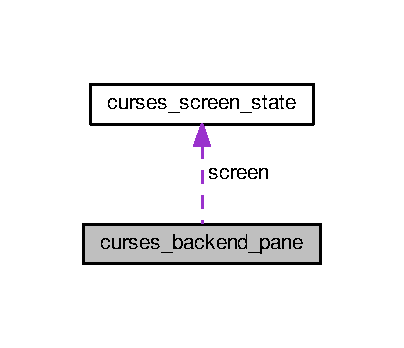
\includegraphics[width=194pt]{structcurses__backend__pane__coll__graph}
\end{center}
\end{figure}
\subsection*{Data Fields}
\begin{DoxyCompactItemize}
\item 
struct \hyperlink{structcurses__screen__state}{curses\+\_\+screen\+\_\+state} \hyperlink{structcurses__backend__pane_a02234fc4e1f0116f10eafc07307be50c}{screen} \mbox{[}\hyperlink{pane_8h_a49f1d9b192f4f01ff444123abde24761a4675b455ce9ebdc1c317e91e0c66e5e0}{T\+Y\+M\+\_\+\+I\+\_\+\+S\+C\+R\+E\+E\+N\+\_\+\+C\+O\+U\+NT}\mbox{]}
\end{DoxyCompactItemize}


\subsection{Detailed Description}


Definition at line 30 of file curses.\+c.



\subsection{Field Documentation}
\mbox{\Hypertarget{structcurses__backend__pane_a02234fc4e1f0116f10eafc07307be50c}\label{structcurses__backend__pane_a02234fc4e1f0116f10eafc07307be50c}} 
\index{curses\+\_\+backend\+\_\+pane@{curses\+\_\+backend\+\_\+pane}!screen@{screen}}
\index{screen@{screen}!curses\+\_\+backend\+\_\+pane@{curses\+\_\+backend\+\_\+pane}}
\subsubsection{\texorpdfstring{screen}{screen}}
{\footnotesize\ttfamily struct \hyperlink{structcurses__screen__state}{curses\+\_\+screen\+\_\+state} curses\+\_\+backend\+\_\+pane\+::screen\mbox{[}\hyperlink{pane_8h_a49f1d9b192f4f01ff444123abde24761a4675b455ce9ebdc1c317e91e0c66e5e0}{T\+Y\+M\+\_\+\+I\+\_\+\+S\+C\+R\+E\+E\+N\+\_\+\+C\+O\+U\+NT}\mbox{]}}



Definition at line 31 of file curses.\+c.



The documentation for this struct was generated from the following file\+:\begin{DoxyCompactItemize}
\item 
src/backend/\hyperlink{curses_8c}{curses.\+c}\end{DoxyCompactItemize}

\hypertarget{structcurses__screen__state}{}\section{curses\+\_\+screen\+\_\+state Struct Reference}
\label{structcurses__screen__state}\index{curses\+\_\+screen\+\_\+state@{curses\+\_\+screen\+\_\+state}}
\subsection*{Data Fields}
\begin{DoxyCompactItemize}
\item 
W\+I\+N\+D\+OW $\ast$ \hyperlink{structcurses__screen__state_a65ce2662ab8c79817e1ec61efa09b6a4}{window}
\end{DoxyCompactItemize}


\subsection{Detailed Description}


Definition at line 26 of file curses.\+c.



\subsection{Field Documentation}
\mbox{\Hypertarget{structcurses__screen__state_a65ce2662ab8c79817e1ec61efa09b6a4}\label{structcurses__screen__state_a65ce2662ab8c79817e1ec61efa09b6a4}} 
\index{curses\+\_\+screen\+\_\+state@{curses\+\_\+screen\+\_\+state}!window@{window}}
\index{window@{window}!curses\+\_\+screen\+\_\+state@{curses\+\_\+screen\+\_\+state}}
\subsubsection{\texorpdfstring{window}{window}}
{\footnotesize\ttfamily W\+I\+N\+D\+OW$\ast$ curses\+\_\+screen\+\_\+state\+::window}



Definition at line 27 of file curses.\+c.



The documentation for this struct was generated from the following file\+:\begin{DoxyCompactItemize}
\item 
src/backend/\hyperlink{curses_8c}{curses.\+c}\end{DoxyCompactItemize}

\hypertarget{structtranslation__table}{}\section{translation\+\_\+table Struct Reference}
\label{structtranslation__table}\index{translation\+\_\+table@{translation\+\_\+table}}


{\ttfamily \#include $<$charset.\+h$>$}

\subsection*{Data Fields}
\begin{DoxyCompactItemize}
\item 
char \hyperlink{structtranslation__table_abc27dc6c1889e84c3b0937bcef5325e9}{table} \mbox{[}\hyperlink{charset_8h_a99fb83031ce9923c84392b4e92f956b5a825d7047f7af75e3411c5c31f489c546}{T\+Y\+M\+\_\+\+I\+\_\+\+T\+R\+A\+N\+S\+L\+A\+T\+I\+O\+N\+\_\+\+T\+A\+B\+L\+E\+\_\+\+S\+I\+ZE}\mbox{]}\mbox{[}\hyperlink{charset_8h_a99fb83031ce9923c84392b4e92f956b5ac96e3ecb3b2dc9625a07967f6b91cf64}{T\+Y\+M\+\_\+\+I\+\_\+\+T\+R\+A\+N\+S\+L\+A\+T\+I\+O\+N\+\_\+\+T\+A\+B\+L\+E\+\_\+\+L\+A\+R\+G\+E\+S\+T\+\_\+\+U\+T\+F8\+\_\+\+C\+H\+A\+R\+A\+C\+T\+E\+R\+\_\+\+S\+E\+Q\+U\+E\+N\+CE}\mbox{]}
\end{DoxyCompactItemize}


\subsection{Detailed Description}


Definition at line 44 of file charset.\+h.



\subsection{Field Documentation}
\mbox{\Hypertarget{structtranslation__table_abc27dc6c1889e84c3b0937bcef5325e9}\label{structtranslation__table_abc27dc6c1889e84c3b0937bcef5325e9}} 
\index{translation\+\_\+table@{translation\+\_\+table}!table@{table}}
\index{table@{table}!translation\+\_\+table@{translation\+\_\+table}}
\subsubsection{\texorpdfstring{table}{table}}
{\footnotesize\ttfamily char translation\+\_\+table\+::table\mbox{[}\hyperlink{charset_8h_a99fb83031ce9923c84392b4e92f956b5a825d7047f7af75e3411c5c31f489c546}{T\+Y\+M\+\_\+\+I\+\_\+\+T\+R\+A\+N\+S\+L\+A\+T\+I\+O\+N\+\_\+\+T\+A\+B\+L\+E\+\_\+\+S\+I\+ZE}\mbox{]}\mbox{[}\hyperlink{charset_8h_a99fb83031ce9923c84392b4e92f956b5ac96e3ecb3b2dc9625a07967f6b91cf64}{T\+Y\+M\+\_\+\+I\+\_\+\+T\+R\+A\+N\+S\+L\+A\+T\+I\+O\+N\+\_\+\+T\+A\+B\+L\+E\+\_\+\+L\+A\+R\+G\+E\+S\+T\+\_\+\+U\+T\+F8\+\_\+\+C\+H\+A\+R\+A\+C\+T\+E\+R\+\_\+\+S\+E\+Q\+U\+E\+N\+CE}\mbox{]}}



Definition at line 45 of file charset.\+h.



The documentation for this struct was generated from the following file\+:\begin{DoxyCompactItemize}
\item 
include/internal/\hyperlink{charset_8h}{charset.\+h}\end{DoxyCompactItemize}

\hypertarget{structtym__absolute__position}{}\section{tym\+\_\+absolute\+\_\+position Struct Reference}
\label{structtym__absolute__position}\index{tym\+\_\+absolute\+\_\+position@{tym\+\_\+absolute\+\_\+position}}


{\ttfamily \#include $<$libttymultiplex.\+h$>$}



Collaboration diagram for tym\+\_\+absolute\+\_\+position\+:
\nopagebreak
\begin{figure}[H]
\begin{center}
\leavevmode
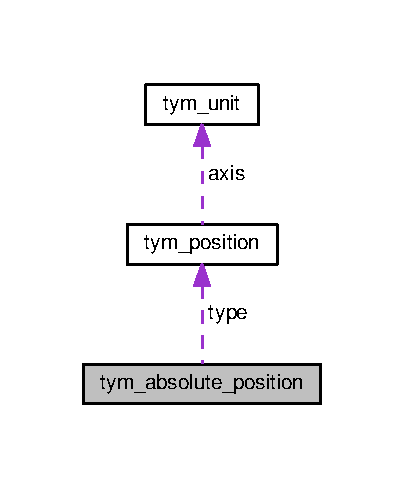
\includegraphics[width=194pt]{structtym__absolute__position__coll__graph}
\end{center}
\end{figure}
\subsection*{Data Fields}
\begin{DoxyCompactItemize}
\item 
struct \hyperlink{structtym__position}{tym\+\_\+position} \hyperlink{structtym__absolute__position_ad80b2993d316f7f166dc1761c1ae65b2}{type} \mbox{[}\hyperlink{libttymultiplex_8h_a23b539c9dc1c137633f8783517fc2653a483bfa59d0a2b43731d992c418a42db7}{T\+Y\+M\+\_\+\+P\+\_\+\+C\+O\+U\+NT}\mbox{]}
\end{DoxyCompactItemize}


\subsection{Detailed Description}


Definition at line 138 of file libttymultiplex.\+h.



\subsection{Field Documentation}
\mbox{\Hypertarget{structtym__absolute__position_ad80b2993d316f7f166dc1761c1ae65b2}\label{structtym__absolute__position_ad80b2993d316f7f166dc1761c1ae65b2}} 
\index{tym\+\_\+absolute\+\_\+position@{tym\+\_\+absolute\+\_\+position}!type@{type}}
\index{type@{type}!tym\+\_\+absolute\+\_\+position@{tym\+\_\+absolute\+\_\+position}}
\subsubsection{\texorpdfstring{type}{type}}
{\footnotesize\ttfamily struct \hyperlink{structtym__position}{tym\+\_\+position} tym\+\_\+absolute\+\_\+position\+::type\mbox{[}\hyperlink{libttymultiplex_8h_a23b539c9dc1c137633f8783517fc2653a483bfa59d0a2b43731d992c418a42db7}{T\+Y\+M\+\_\+\+P\+\_\+\+C\+O\+U\+NT}\mbox{]}}



Definition at line 138 of file libttymultiplex.\+h.



The documentation for this struct was generated from the following file\+:\begin{DoxyCompactItemize}
\item 
include/\hyperlink{libttymultiplex_8h}{libttymultiplex.\+h}\end{DoxyCompactItemize}

\hypertarget{structtym__absolute__position__rectangle}{}\section{tym\+\_\+absolute\+\_\+position\+\_\+rectangle Struct Reference}
\label{structtym__absolute__position__rectangle}\index{tym\+\_\+absolute\+\_\+position\+\_\+rectangle@{tym\+\_\+absolute\+\_\+position\+\_\+rectangle}}


{\ttfamily \#include $<$libttymultiplex.\+h$>$}



Collaboration diagram for tym\+\_\+absolute\+\_\+position\+\_\+rectangle\+:
\nopagebreak
\begin{figure}[H]
\begin{center}
\leavevmode
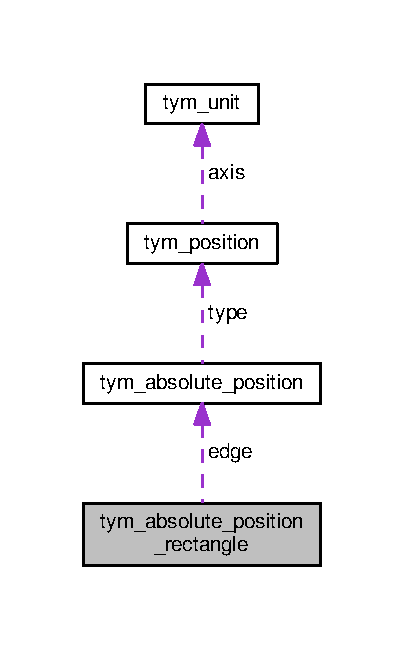
\includegraphics[width=194pt]{structtym__absolute__position__rectangle__coll__graph}
\end{center}
\end{figure}
\subsection*{Data Fields}
\begin{DoxyCompactItemize}
\item 
struct \hyperlink{structtym__absolute__position}{tym\+\_\+absolute\+\_\+position} \hyperlink{structtym__absolute__position__rectangle_a8ae5bbbd49e8293d8fa93df8d1572423}{edge} \mbox{[}\hyperlink{libttymultiplex_8h_ad8856480bf629c72938051528100b834ac0bfa9550b58bc257ca09715d719de7f}{T\+Y\+M\+\_\+\+E\+D\+G\+E\+\_\+\+C\+O\+U\+NT}\mbox{]}
\end{DoxyCompactItemize}


\subsection{Detailed Description}


Definition at line 138 of file libttymultiplex.\+h.



\subsection{Field Documentation}
\mbox{\Hypertarget{structtym__absolute__position__rectangle_a8ae5bbbd49e8293d8fa93df8d1572423}\label{structtym__absolute__position__rectangle_a8ae5bbbd49e8293d8fa93df8d1572423}} 
\index{tym\+\_\+absolute\+\_\+position\+\_\+rectangle@{tym\+\_\+absolute\+\_\+position\+\_\+rectangle}!edge@{edge}}
\index{edge@{edge}!tym\+\_\+absolute\+\_\+position\+\_\+rectangle@{tym\+\_\+absolute\+\_\+position\+\_\+rectangle}}
\subsubsection{\texorpdfstring{edge}{edge}}
{\footnotesize\ttfamily struct \hyperlink{structtym__absolute__position}{tym\+\_\+absolute\+\_\+position} tym\+\_\+absolute\+\_\+position\+\_\+rectangle\+::edge\mbox{[}\hyperlink{libttymultiplex_8h_ad8856480bf629c72938051528100b834ac0bfa9550b58bc257ca09715d719de7f}{T\+Y\+M\+\_\+\+E\+D\+G\+E\+\_\+\+C\+O\+U\+NT}\mbox{]}}



Definition at line 138 of file libttymultiplex.\+h.



The documentation for this struct was generated from the following file\+:\begin{DoxyCompactItemize}
\item 
include/\hyperlink{libttymultiplex_8h}{libttymultiplex.\+h}\end{DoxyCompactItemize}

\hypertarget{structtym__i__backend}{}\section{tym\+\_\+i\+\_\+backend Struct Reference}
\label{structtym__i__backend}\index{tym\+\_\+i\+\_\+backend@{tym\+\_\+i\+\_\+backend}}


{\ttfamily \#include $<$backend.\+h$>$}



Collaboration diagram for tym\+\_\+i\+\_\+backend\+:
\nopagebreak
\begin{figure}[H]
\begin{center}
\leavevmode
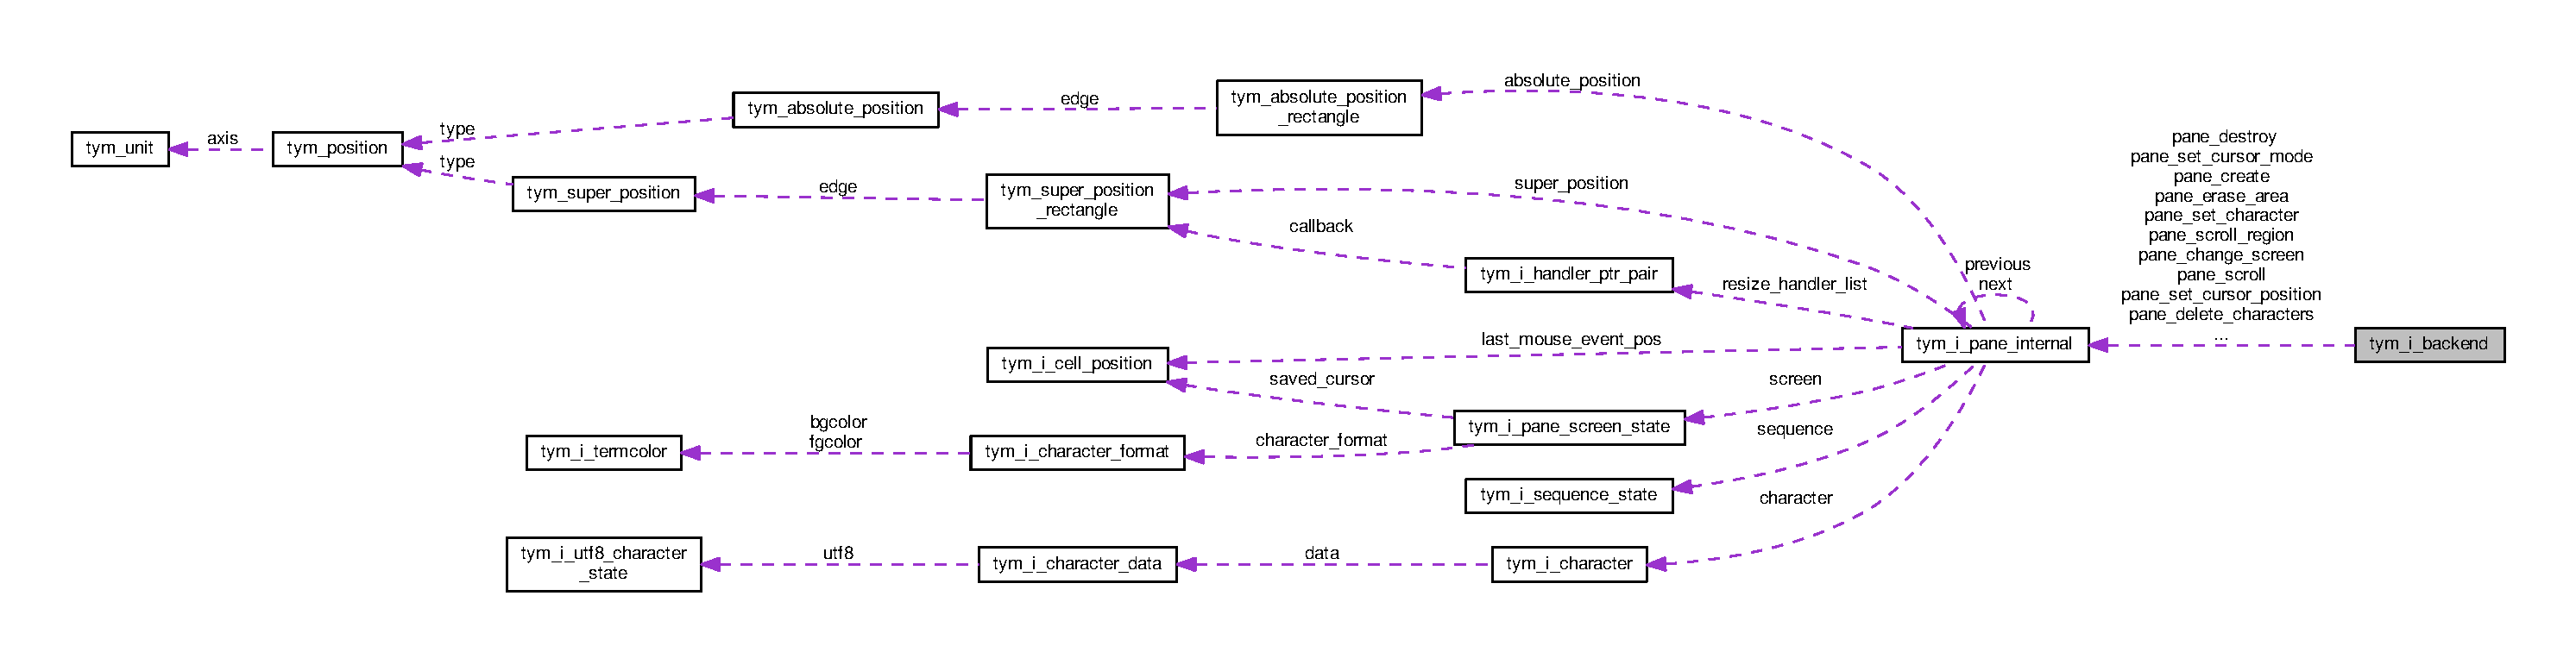
\includegraphics[width=350pt]{structtym__i__backend__coll__graph}
\end{center}
\end{figure}
\subsection*{Data Fields}
\begin{DoxyCompactItemize}
\item 
\hyperlink{backend_8h_a1d8c83e098af07295e7c8c6aaff509f8}{tym\+\_\+i\+\_\+init\+\_\+proc} \hyperlink{structtym__i__backend_a9e5755b91dadb2460eb67423e126cf60}{init}
\item 
\hyperlink{backend_8h_a71c0f80d2ad6f4c617855bed5f727832}{tym\+\_\+i\+\_\+cleanup\+\_\+proc} \hyperlink{structtym__i__backend_af3dd909e074449e20489addd04a9409b}{cleanup}
\item 
\hyperlink{backend_8h_a969a37c5dad74fed827c63879a3ea594}{tym\+\_\+i\+\_\+resize\+\_\+proc} \hyperlink{structtym__i__backend_a6a9798091f83b97b02c2765ab9ab7f5b}{resize}
\item 
\hyperlink{backend_8h_ab44c405291766aa8377ccabbf142c682}{tym\+\_\+i\+\_\+pane\+\_\+create\+\_\+proc} \hyperlink{structtym__i__backend_ac09a0c208115068effc8a0de70136c63}{pane\+\_\+create}
\item 
\hyperlink{backend_8h_a7c52fa9848f5daacdca285c8e25c6daf}{tym\+\_\+i\+\_\+pane\+\_\+destroy\+\_\+proc} \hyperlink{structtym__i__backend_a26f012c047a54997dbfd52868c723fe5}{pane\+\_\+destroy}
\item 
\hyperlink{backend_8h_ae66adc784ab9e9adcb7f43713798b754}{tym\+\_\+i\+\_\+pane\+\_\+resize\+\_\+proc} \hyperlink{structtym__i__backend_a625938e1dcc5d0b40561b42c0d37a794}{pane\+\_\+resize}
\item 
\hyperlink{backend_8h_a8f701dd0984f9c7aa9f76fcd2df15a27}{tym\+\_\+i\+\_\+pane\+\_\+scroll\+\_\+region\+\_\+proc} \hyperlink{structtym__i__backend_a995d60cb63fc0ac13220fda8628c4267}{pane\+\_\+scroll\+\_\+region}
\item 
\hyperlink{backend_8h_af5c21e9bc7ce1861a821cf0b8f3baa24}{tym\+\_\+i\+\_\+pane\+\_\+set\+\_\+cursor\+\_\+position\+\_\+proc} \hyperlink{structtym__i__backend_a6422b6a50ad3afbc5732bbef76953ac7}{pane\+\_\+set\+\_\+cursor\+\_\+position}
\item 
\hyperlink{backend_8h_a4a3d0bb3b2fb6baa1f86e39770756a18}{tym\+\_\+i\+\_\+pane\+\_\+set\+\_\+character\+\_\+proc} \hyperlink{structtym__i__backend_a0840c9980f7b7de92870d92787199940}{pane\+\_\+set\+\_\+character}
\item 
\hyperlink{backend_8h_a0926d88cba57a1e598f92df346d9d6a3}{tym\+\_\+i\+\_\+pane\+\_\+delete\+\_\+characters\+\_\+proc} \hyperlink{structtym__i__backend_a7c0e3c008f7c54c8c6f232cdde226a38}{pane\+\_\+delete\+\_\+characters}
\item 
\hyperlink{backend_8h_a99b50ea4d7c5349b4df1e879b2140a97}{tym\+\_\+i\+\_\+pane\+\_\+refresh\+\_\+proc} \hyperlink{structtym__i__backend_af190f73df64b296e3af5dfea90e560b4}{pane\+\_\+refresh}
\item 
\hyperlink{backend_8h_a9488390b6c0e8e6ee6df0f65c0600033}{tym\+\_\+i\+\_\+pane\+\_\+set\+\_\+cursor\+\_\+mode\+\_\+proc} \hyperlink{structtym__i__backend_abc77f840a378d769e117033440faa961}{pane\+\_\+set\+\_\+cursor\+\_\+mode}
\item 
\hyperlink{backend_8h_ab44bedb286c42c2994bf88375e64176f}{tym\+\_\+i\+\_\+pane\+\_\+scroll\+\_\+proc} \hyperlink{structtym__i__backend_aa1f08a3ae4b68a6b987c928a091ff80f}{pane\+\_\+scroll}
\item 
\hyperlink{backend_8h_a61a3d2bde17cca99666001e082332bc4}{tym\+\_\+i\+\_\+pane\+\_\+erase\+\_\+area\+\_\+proc} \hyperlink{structtym__i__backend_a81be791bdd6da6b01bb8f85b8388707c}{pane\+\_\+erase\+\_\+area}
\item 
\hyperlink{backend_8h_a069b99db5129d301726cec915fea32a8}{tym\+\_\+i\+\_\+pane\+\_\+change\+\_\+screen\+\_\+proc} \hyperlink{structtym__i__backend_a75f72684565b37e6ca66f5f71260931b}{pane\+\_\+change\+\_\+screen}
\item 
\hyperlink{backend_8h_aaaee2104d442c8976abfd9228375c878}{tym\+\_\+i\+\_\+pane\+\_\+set\+\_\+area\+\_\+to\+\_\+character\+\_\+proc} \hyperlink{structtym__i__backend_ab943a3203b09c330b09fa8c9a50b7cbf}{pane\+\_\+set\+\_\+area\+\_\+to\+\_\+character}
\end{DoxyCompactItemize}


\subsection{Detailed Description}


Definition at line 65 of file backend.\+h.



\subsection{Field Documentation}
\mbox{\Hypertarget{structtym__i__backend_af3dd909e074449e20489addd04a9409b}\label{structtym__i__backend_af3dd909e074449e20489addd04a9409b}} 
\index{tym\+\_\+i\+\_\+backend@{tym\+\_\+i\+\_\+backend}!cleanup@{cleanup}}
\index{cleanup@{cleanup}!tym\+\_\+i\+\_\+backend@{tym\+\_\+i\+\_\+backend}}
\subsubsection{\texorpdfstring{cleanup}{cleanup}}
{\footnotesize\ttfamily \hyperlink{backend_8h_a71c0f80d2ad6f4c617855bed5f727832}{tym\+\_\+i\+\_\+cleanup\+\_\+proc} tym\+\_\+i\+\_\+backend\+::cleanup}



Definition at line 68 of file backend.\+h.

\mbox{\Hypertarget{structtym__i__backend_a9e5755b91dadb2460eb67423e126cf60}\label{structtym__i__backend_a9e5755b91dadb2460eb67423e126cf60}} 
\index{tym\+\_\+i\+\_\+backend@{tym\+\_\+i\+\_\+backend}!init@{init}}
\index{init@{init}!tym\+\_\+i\+\_\+backend@{tym\+\_\+i\+\_\+backend}}
\subsubsection{\texorpdfstring{init}{init}}
{\footnotesize\ttfamily \hyperlink{backend_8h_a1d8c83e098af07295e7c8c6aaff509f8}{tym\+\_\+i\+\_\+init\+\_\+proc} tym\+\_\+i\+\_\+backend\+::init}



Definition at line 68 of file backend.\+h.

\mbox{\Hypertarget{structtym__i__backend_a75f72684565b37e6ca66f5f71260931b}\label{structtym__i__backend_a75f72684565b37e6ca66f5f71260931b}} 
\index{tym\+\_\+i\+\_\+backend@{tym\+\_\+i\+\_\+backend}!pane\+\_\+change\+\_\+screen@{pane\+\_\+change\+\_\+screen}}
\index{pane\+\_\+change\+\_\+screen@{pane\+\_\+change\+\_\+screen}!tym\+\_\+i\+\_\+backend@{tym\+\_\+i\+\_\+backend}}
\subsubsection{\texorpdfstring{pane\+\_\+change\+\_\+screen}{pane\_change\_screen}}
{\footnotesize\ttfamily \hyperlink{backend_8h_a069b99db5129d301726cec915fea32a8}{tym\+\_\+i\+\_\+pane\+\_\+change\+\_\+screen\+\_\+proc} tym\+\_\+i\+\_\+backend\+::pane\+\_\+change\+\_\+screen}



Definition at line 68 of file backend.\+h.

\mbox{\Hypertarget{structtym__i__backend_ac09a0c208115068effc8a0de70136c63}\label{structtym__i__backend_ac09a0c208115068effc8a0de70136c63}} 
\index{tym\+\_\+i\+\_\+backend@{tym\+\_\+i\+\_\+backend}!pane\+\_\+create@{pane\+\_\+create}}
\index{pane\+\_\+create@{pane\+\_\+create}!tym\+\_\+i\+\_\+backend@{tym\+\_\+i\+\_\+backend}}
\subsubsection{\texorpdfstring{pane\+\_\+create}{pane\_create}}
{\footnotesize\ttfamily \hyperlink{backend_8h_ab44c405291766aa8377ccabbf142c682}{tym\+\_\+i\+\_\+pane\+\_\+create\+\_\+proc} tym\+\_\+i\+\_\+backend\+::pane\+\_\+create}



Definition at line 68 of file backend.\+h.

\mbox{\Hypertarget{structtym__i__backend_a7c0e3c008f7c54c8c6f232cdde226a38}\label{structtym__i__backend_a7c0e3c008f7c54c8c6f232cdde226a38}} 
\index{tym\+\_\+i\+\_\+backend@{tym\+\_\+i\+\_\+backend}!pane\+\_\+delete\+\_\+characters@{pane\+\_\+delete\+\_\+characters}}
\index{pane\+\_\+delete\+\_\+characters@{pane\+\_\+delete\+\_\+characters}!tym\+\_\+i\+\_\+backend@{tym\+\_\+i\+\_\+backend}}
\subsubsection{\texorpdfstring{pane\+\_\+delete\+\_\+characters}{pane\_delete\_characters}}
{\footnotesize\ttfamily \hyperlink{backend_8h_a0926d88cba57a1e598f92df346d9d6a3}{tym\+\_\+i\+\_\+pane\+\_\+delete\+\_\+characters\+\_\+proc} tym\+\_\+i\+\_\+backend\+::pane\+\_\+delete\+\_\+characters}



Definition at line 68 of file backend.\+h.

\mbox{\Hypertarget{structtym__i__backend_a26f012c047a54997dbfd52868c723fe5}\label{structtym__i__backend_a26f012c047a54997dbfd52868c723fe5}} 
\index{tym\+\_\+i\+\_\+backend@{tym\+\_\+i\+\_\+backend}!pane\+\_\+destroy@{pane\+\_\+destroy}}
\index{pane\+\_\+destroy@{pane\+\_\+destroy}!tym\+\_\+i\+\_\+backend@{tym\+\_\+i\+\_\+backend}}
\subsubsection{\texorpdfstring{pane\+\_\+destroy}{pane\_destroy}}
{\footnotesize\ttfamily \hyperlink{backend_8h_a7c52fa9848f5daacdca285c8e25c6daf}{tym\+\_\+i\+\_\+pane\+\_\+destroy\+\_\+proc} tym\+\_\+i\+\_\+backend\+::pane\+\_\+destroy}



Definition at line 68 of file backend.\+h.

\mbox{\Hypertarget{structtym__i__backend_a81be791bdd6da6b01bb8f85b8388707c}\label{structtym__i__backend_a81be791bdd6da6b01bb8f85b8388707c}} 
\index{tym\+\_\+i\+\_\+backend@{tym\+\_\+i\+\_\+backend}!pane\+\_\+erase\+\_\+area@{pane\+\_\+erase\+\_\+area}}
\index{pane\+\_\+erase\+\_\+area@{pane\+\_\+erase\+\_\+area}!tym\+\_\+i\+\_\+backend@{tym\+\_\+i\+\_\+backend}}
\subsubsection{\texorpdfstring{pane\+\_\+erase\+\_\+area}{pane\_erase\_area}}
{\footnotesize\ttfamily \hyperlink{backend_8h_a61a3d2bde17cca99666001e082332bc4}{tym\+\_\+i\+\_\+pane\+\_\+erase\+\_\+area\+\_\+proc} tym\+\_\+i\+\_\+backend\+::pane\+\_\+erase\+\_\+area}



Definition at line 68 of file backend.\+h.

\mbox{\Hypertarget{structtym__i__backend_af190f73df64b296e3af5dfea90e560b4}\label{structtym__i__backend_af190f73df64b296e3af5dfea90e560b4}} 
\index{tym\+\_\+i\+\_\+backend@{tym\+\_\+i\+\_\+backend}!pane\+\_\+refresh@{pane\+\_\+refresh}}
\index{pane\+\_\+refresh@{pane\+\_\+refresh}!tym\+\_\+i\+\_\+backend@{tym\+\_\+i\+\_\+backend}}
\subsubsection{\texorpdfstring{pane\+\_\+refresh}{pane\_refresh}}
{\footnotesize\ttfamily \hyperlink{backend_8h_a99b50ea4d7c5349b4df1e879b2140a97}{tym\+\_\+i\+\_\+pane\+\_\+refresh\+\_\+proc} tym\+\_\+i\+\_\+backend\+::pane\+\_\+refresh}



Definition at line 68 of file backend.\+h.

\mbox{\Hypertarget{structtym__i__backend_a625938e1dcc5d0b40561b42c0d37a794}\label{structtym__i__backend_a625938e1dcc5d0b40561b42c0d37a794}} 
\index{tym\+\_\+i\+\_\+backend@{tym\+\_\+i\+\_\+backend}!pane\+\_\+resize@{pane\+\_\+resize}}
\index{pane\+\_\+resize@{pane\+\_\+resize}!tym\+\_\+i\+\_\+backend@{tym\+\_\+i\+\_\+backend}}
\subsubsection{\texorpdfstring{pane\+\_\+resize}{pane\_resize}}
{\footnotesize\ttfamily \hyperlink{backend_8h_ae66adc784ab9e9adcb7f43713798b754}{tym\+\_\+i\+\_\+pane\+\_\+resize\+\_\+proc} tym\+\_\+i\+\_\+backend\+::pane\+\_\+resize}



Definition at line 68 of file backend.\+h.

\mbox{\Hypertarget{structtym__i__backend_aa1f08a3ae4b68a6b987c928a091ff80f}\label{structtym__i__backend_aa1f08a3ae4b68a6b987c928a091ff80f}} 
\index{tym\+\_\+i\+\_\+backend@{tym\+\_\+i\+\_\+backend}!pane\+\_\+scroll@{pane\+\_\+scroll}}
\index{pane\+\_\+scroll@{pane\+\_\+scroll}!tym\+\_\+i\+\_\+backend@{tym\+\_\+i\+\_\+backend}}
\subsubsection{\texorpdfstring{pane\+\_\+scroll}{pane\_scroll}}
{\footnotesize\ttfamily \hyperlink{backend_8h_ab44bedb286c42c2994bf88375e64176f}{tym\+\_\+i\+\_\+pane\+\_\+scroll\+\_\+proc} tym\+\_\+i\+\_\+backend\+::pane\+\_\+scroll}



Definition at line 68 of file backend.\+h.

\mbox{\Hypertarget{structtym__i__backend_a995d60cb63fc0ac13220fda8628c4267}\label{structtym__i__backend_a995d60cb63fc0ac13220fda8628c4267}} 
\index{tym\+\_\+i\+\_\+backend@{tym\+\_\+i\+\_\+backend}!pane\+\_\+scroll\+\_\+region@{pane\+\_\+scroll\+\_\+region}}
\index{pane\+\_\+scroll\+\_\+region@{pane\+\_\+scroll\+\_\+region}!tym\+\_\+i\+\_\+backend@{tym\+\_\+i\+\_\+backend}}
\subsubsection{\texorpdfstring{pane\+\_\+scroll\+\_\+region}{pane\_scroll\_region}}
{\footnotesize\ttfamily \hyperlink{backend_8h_a8f701dd0984f9c7aa9f76fcd2df15a27}{tym\+\_\+i\+\_\+pane\+\_\+scroll\+\_\+region\+\_\+proc} tym\+\_\+i\+\_\+backend\+::pane\+\_\+scroll\+\_\+region}



Definition at line 68 of file backend.\+h.

\mbox{\Hypertarget{structtym__i__backend_ab943a3203b09c330b09fa8c9a50b7cbf}\label{structtym__i__backend_ab943a3203b09c330b09fa8c9a50b7cbf}} 
\index{tym\+\_\+i\+\_\+backend@{tym\+\_\+i\+\_\+backend}!pane\+\_\+set\+\_\+area\+\_\+to\+\_\+character@{pane\+\_\+set\+\_\+area\+\_\+to\+\_\+character}}
\index{pane\+\_\+set\+\_\+area\+\_\+to\+\_\+character@{pane\+\_\+set\+\_\+area\+\_\+to\+\_\+character}!tym\+\_\+i\+\_\+backend@{tym\+\_\+i\+\_\+backend}}
\subsubsection{\texorpdfstring{pane\+\_\+set\+\_\+area\+\_\+to\+\_\+character}{pane\_set\_area\_to\_character}}
{\footnotesize\ttfamily \hyperlink{backend_8h_aaaee2104d442c8976abfd9228375c878}{tym\+\_\+i\+\_\+pane\+\_\+set\+\_\+area\+\_\+to\+\_\+character\+\_\+proc} tym\+\_\+i\+\_\+backend\+::pane\+\_\+set\+\_\+area\+\_\+to\+\_\+character}



Definition at line 68 of file backend.\+h.

\mbox{\Hypertarget{structtym__i__backend_a0840c9980f7b7de92870d92787199940}\label{structtym__i__backend_a0840c9980f7b7de92870d92787199940}} 
\index{tym\+\_\+i\+\_\+backend@{tym\+\_\+i\+\_\+backend}!pane\+\_\+set\+\_\+character@{pane\+\_\+set\+\_\+character}}
\index{pane\+\_\+set\+\_\+character@{pane\+\_\+set\+\_\+character}!tym\+\_\+i\+\_\+backend@{tym\+\_\+i\+\_\+backend}}
\subsubsection{\texorpdfstring{pane\+\_\+set\+\_\+character}{pane\_set\_character}}
{\footnotesize\ttfamily \hyperlink{backend_8h_a4a3d0bb3b2fb6baa1f86e39770756a18}{tym\+\_\+i\+\_\+pane\+\_\+set\+\_\+character\+\_\+proc} tym\+\_\+i\+\_\+backend\+::pane\+\_\+set\+\_\+character}



Definition at line 68 of file backend.\+h.

\mbox{\Hypertarget{structtym__i__backend_abc77f840a378d769e117033440faa961}\label{structtym__i__backend_abc77f840a378d769e117033440faa961}} 
\index{tym\+\_\+i\+\_\+backend@{tym\+\_\+i\+\_\+backend}!pane\+\_\+set\+\_\+cursor\+\_\+mode@{pane\+\_\+set\+\_\+cursor\+\_\+mode}}
\index{pane\+\_\+set\+\_\+cursor\+\_\+mode@{pane\+\_\+set\+\_\+cursor\+\_\+mode}!tym\+\_\+i\+\_\+backend@{tym\+\_\+i\+\_\+backend}}
\subsubsection{\texorpdfstring{pane\+\_\+set\+\_\+cursor\+\_\+mode}{pane\_set\_cursor\_mode}}
{\footnotesize\ttfamily \hyperlink{backend_8h_a9488390b6c0e8e6ee6df0f65c0600033}{tym\+\_\+i\+\_\+pane\+\_\+set\+\_\+cursor\+\_\+mode\+\_\+proc} tym\+\_\+i\+\_\+backend\+::pane\+\_\+set\+\_\+cursor\+\_\+mode}



Definition at line 68 of file backend.\+h.

\mbox{\Hypertarget{structtym__i__backend_a6422b6a50ad3afbc5732bbef76953ac7}\label{structtym__i__backend_a6422b6a50ad3afbc5732bbef76953ac7}} 
\index{tym\+\_\+i\+\_\+backend@{tym\+\_\+i\+\_\+backend}!pane\+\_\+set\+\_\+cursor\+\_\+position@{pane\+\_\+set\+\_\+cursor\+\_\+position}}
\index{pane\+\_\+set\+\_\+cursor\+\_\+position@{pane\+\_\+set\+\_\+cursor\+\_\+position}!tym\+\_\+i\+\_\+backend@{tym\+\_\+i\+\_\+backend}}
\subsubsection{\texorpdfstring{pane\+\_\+set\+\_\+cursor\+\_\+position}{pane\_set\_cursor\_position}}
{\footnotesize\ttfamily \hyperlink{backend_8h_af5c21e9bc7ce1861a821cf0b8f3baa24}{tym\+\_\+i\+\_\+pane\+\_\+set\+\_\+cursor\+\_\+position\+\_\+proc} tym\+\_\+i\+\_\+backend\+::pane\+\_\+set\+\_\+cursor\+\_\+position}



Definition at line 68 of file backend.\+h.

\mbox{\Hypertarget{structtym__i__backend_a6a9798091f83b97b02c2765ab9ab7f5b}\label{structtym__i__backend_a6a9798091f83b97b02c2765ab9ab7f5b}} 
\index{tym\+\_\+i\+\_\+backend@{tym\+\_\+i\+\_\+backend}!resize@{resize}}
\index{resize@{resize}!tym\+\_\+i\+\_\+backend@{tym\+\_\+i\+\_\+backend}}
\subsubsection{\texorpdfstring{resize}{resize}}
{\footnotesize\ttfamily \hyperlink{backend_8h_a969a37c5dad74fed827c63879a3ea594}{tym\+\_\+i\+\_\+resize\+\_\+proc} tym\+\_\+i\+\_\+backend\+::resize}



Definition at line 68 of file backend.\+h.



The documentation for this struct was generated from the following file\+:\begin{DoxyCompactItemize}
\item 
include/internal/\hyperlink{backend_8h}{backend.\+h}\end{DoxyCompactItemize}

\hypertarget{structtym__i__backend__entry}{}\section{tym\+\_\+i\+\_\+backend\+\_\+entry Struct Reference}
\label{structtym__i__backend__entry}\index{tym\+\_\+i\+\_\+backend\+\_\+entry@{tym\+\_\+i\+\_\+backend\+\_\+entry}}


{\ttfamily \#include $<$backend.\+h$>$}



Collaboration diagram for tym\+\_\+i\+\_\+backend\+\_\+entry\+:
\nopagebreak
\begin{figure}[H]
\begin{center}
\leavevmode
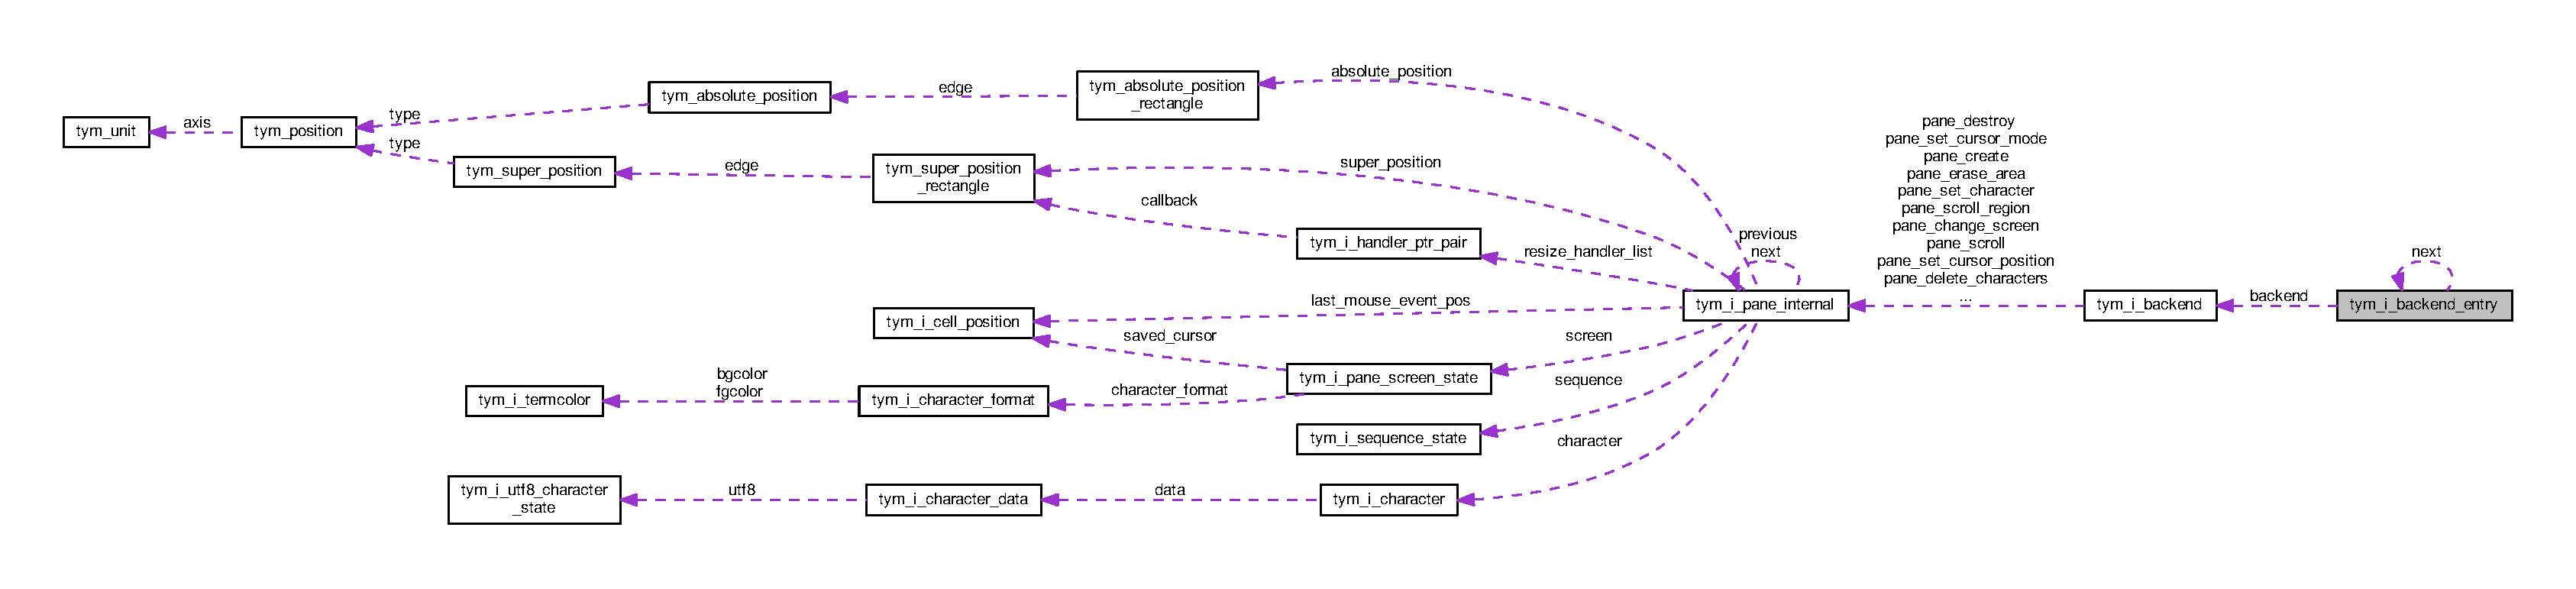
\includegraphics[width=350pt]{structtym__i__backend__entry__coll__graph}
\end{center}
\end{figure}
\subsection*{Data Fields}
\begin{DoxyCompactItemize}
\item 
const char $\ast$ \hyperlink{structtym__i__backend__entry_abc39107ed565fd8c35370447417eedfc}{name}
\item 
struct \hyperlink{structtym__i__backend}{tym\+\_\+i\+\_\+backend} \hyperlink{structtym__i__backend__entry_a4b704ae50db3e520c36d3fa75e93b28c}{backend}
\item 
const struct \hyperlink{structtym__i__backend__entry}{tym\+\_\+i\+\_\+backend\+\_\+entry} $\ast$ \hyperlink{structtym__i__backend__entry_a52978e3325ccdb0f6bcf2bb98e457872}{next}
\end{DoxyCompactItemize}


\subsection{Detailed Description}


Definition at line 73 of file backend.\+h.



\subsection{Field Documentation}
\mbox{\Hypertarget{structtym__i__backend__entry_a4b704ae50db3e520c36d3fa75e93b28c}\label{structtym__i__backend__entry_a4b704ae50db3e520c36d3fa75e93b28c}} 
\index{tym\+\_\+i\+\_\+backend\+\_\+entry@{tym\+\_\+i\+\_\+backend\+\_\+entry}!backend@{backend}}
\index{backend@{backend}!tym\+\_\+i\+\_\+backend\+\_\+entry@{tym\+\_\+i\+\_\+backend\+\_\+entry}}
\subsubsection{\texorpdfstring{backend}{backend}}
{\footnotesize\ttfamily struct \hyperlink{structtym__i__backend}{tym\+\_\+i\+\_\+backend} tym\+\_\+i\+\_\+backend\+\_\+entry\+::backend}



Definition at line 75 of file backend.\+h.

\mbox{\Hypertarget{structtym__i__backend__entry_abc39107ed565fd8c35370447417eedfc}\label{structtym__i__backend__entry_abc39107ed565fd8c35370447417eedfc}} 
\index{tym\+\_\+i\+\_\+backend\+\_\+entry@{tym\+\_\+i\+\_\+backend\+\_\+entry}!name@{name}}
\index{name@{name}!tym\+\_\+i\+\_\+backend\+\_\+entry@{tym\+\_\+i\+\_\+backend\+\_\+entry}}
\subsubsection{\texorpdfstring{name}{name}}
{\footnotesize\ttfamily const char$\ast$ tym\+\_\+i\+\_\+backend\+\_\+entry\+::name}



Definition at line 74 of file backend.\+h.

\mbox{\Hypertarget{structtym__i__backend__entry_a52978e3325ccdb0f6bcf2bb98e457872}\label{structtym__i__backend__entry_a52978e3325ccdb0f6bcf2bb98e457872}} 
\index{tym\+\_\+i\+\_\+backend\+\_\+entry@{tym\+\_\+i\+\_\+backend\+\_\+entry}!next@{next}}
\index{next@{next}!tym\+\_\+i\+\_\+backend\+\_\+entry@{tym\+\_\+i\+\_\+backend\+\_\+entry}}
\subsubsection{\texorpdfstring{next}{next}}
{\footnotesize\ttfamily const struct \hyperlink{structtym__i__backend__entry}{tym\+\_\+i\+\_\+backend\+\_\+entry}$\ast$ tym\+\_\+i\+\_\+backend\+\_\+entry\+::next}



Definition at line 76 of file backend.\+h.



The documentation for this struct was generated from the following file\+:\begin{DoxyCompactItemize}
\item 
include/internal/\hyperlink{backend_8h}{backend.\+h}\end{DoxyCompactItemize}

\hypertarget{structtym__i__cell__position}{}\section{tym\+\_\+i\+\_\+cell\+\_\+position Struct Reference}
\label{structtym__i__cell__position}\index{tym\+\_\+i\+\_\+cell\+\_\+position@{tym\+\_\+i\+\_\+cell\+\_\+position}}


{\ttfamily \#include $<$pane.\+h$>$}

\subsection*{Data Fields}
\begin{DoxyCompactItemize}
\item 
unsigned \hyperlink{structtym__i__cell__position_a6481c197b637d226dfbf3bcaf771bab5}{x}
\item 
unsigned \hyperlink{structtym__i__cell__position_a82542ee37778b609c1e1ab7043938358}{y}
\end{DoxyCompactItemize}


\subsection{Detailed Description}


Definition at line 109 of file pane.\+h.



\subsection{Field Documentation}
\mbox{\Hypertarget{structtym__i__cell__position_a6481c197b637d226dfbf3bcaf771bab5}\label{structtym__i__cell__position_a6481c197b637d226dfbf3bcaf771bab5}} 
\index{tym\+\_\+i\+\_\+cell\+\_\+position@{tym\+\_\+i\+\_\+cell\+\_\+position}!x@{x}}
\index{x@{x}!tym\+\_\+i\+\_\+cell\+\_\+position@{tym\+\_\+i\+\_\+cell\+\_\+position}}
\subsubsection{\texorpdfstring{x}{x}}
{\footnotesize\ttfamily unsigned tym\+\_\+i\+\_\+cell\+\_\+position\+::x}



Definition at line 110 of file pane.\+h.

\mbox{\Hypertarget{structtym__i__cell__position_a82542ee37778b609c1e1ab7043938358}\label{structtym__i__cell__position_a82542ee37778b609c1e1ab7043938358}} 
\index{tym\+\_\+i\+\_\+cell\+\_\+position@{tym\+\_\+i\+\_\+cell\+\_\+position}!y@{y}}
\index{y@{y}!tym\+\_\+i\+\_\+cell\+\_\+position@{tym\+\_\+i\+\_\+cell\+\_\+position}}
\subsubsection{\texorpdfstring{y}{y}}
{\footnotesize\ttfamily unsigned tym\+\_\+i\+\_\+cell\+\_\+position\+::y}



Definition at line 110 of file pane.\+h.



The documentation for this struct was generated from the following file\+:\begin{DoxyCompactItemize}
\item 
include/internal/\hyperlink{pane_8h}{pane.\+h}\end{DoxyCompactItemize}

\hypertarget{structtym__i__character}{}\section{tym\+\_\+i\+\_\+character Struct Reference}
\label{structtym__i__character}\index{tym\+\_\+i\+\_\+character@{tym\+\_\+i\+\_\+character}}


{\ttfamily \#include $<$pane.\+h$>$}



Collaboration diagram for tym\+\_\+i\+\_\+character\+:
\nopagebreak
\begin{figure}[H]
\begin{center}
\leavevmode
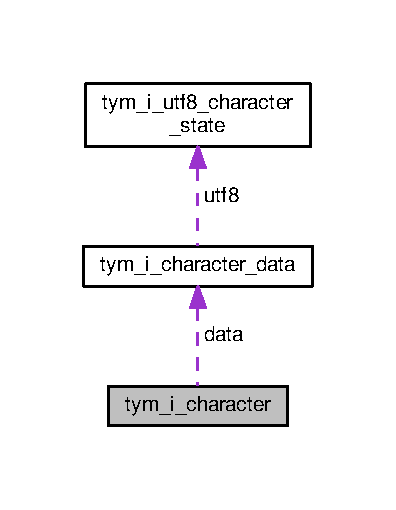
\includegraphics[width=190pt]{structtym__i__character__coll__graph}
\end{center}
\end{figure}
\subsection*{Data Fields}
\begin{DoxyCompactItemize}
\item 
enum \hyperlink{charset_8h_ac56946240a6c0621eb2162e6a7e85493}{charset\+\_\+selection} \hyperlink{structtym__i__character_a03e1385411863f05f23f05aa453db5f6}{charset\+\_\+selection}
\item 
bool \hyperlink{structtym__i__character_a4dd1b66f6a453c6b7243d51549b27160}{not\+\_\+utf8}
\item 
enum \hyperlink{charset_8h_aec311a13b718c6327abd094839df7146}{tym\+\_\+i\+\_\+charset\+\_\+type} \hyperlink{structtym__i__character_a6cc0f4a423aacfba65d2b9df6109ac03}{charset\+\_\+g} \mbox{[}\hyperlink{pane_8h_a0411cd49bb5b71852cecd93bcbf0ca2da4d2fa1719aa429e38bbd477d3a38634b}{T\+Y\+M\+\_\+\+I\+\_\+\+G\+\_\+\+C\+H\+A\+R\+S\+E\+T\+\_\+\+C\+O\+U\+NT}\mbox{]}
\item 
union \hyperlink{uniontym__i__character__data}{tym\+\_\+i\+\_\+character\+\_\+data} \hyperlink{structtym__i__character_aa38c672dcb8dba6d8f651132ae2655b3}{data}
\end{DoxyCompactItemize}


\subsection{Detailed Description}


Definition at line 118 of file pane.\+h.



\subsection{Field Documentation}
\mbox{\Hypertarget{structtym__i__character_a6cc0f4a423aacfba65d2b9df6109ac03}\label{structtym__i__character_a6cc0f4a423aacfba65d2b9df6109ac03}} 
\index{tym\+\_\+i\+\_\+character@{tym\+\_\+i\+\_\+character}!charset\+\_\+g@{charset\+\_\+g}}
\index{charset\+\_\+g@{charset\+\_\+g}!tym\+\_\+i\+\_\+character@{tym\+\_\+i\+\_\+character}}
\subsubsection{\texorpdfstring{charset\+\_\+g}{charset\_g}}
{\footnotesize\ttfamily enum \hyperlink{charset_8h_aec311a13b718c6327abd094839df7146}{tym\+\_\+i\+\_\+charset\+\_\+type} tym\+\_\+i\+\_\+character\+::charset\+\_\+g\mbox{[}\hyperlink{pane_8h_a0411cd49bb5b71852cecd93bcbf0ca2da4d2fa1719aa429e38bbd477d3a38634b}{T\+Y\+M\+\_\+\+I\+\_\+\+G\+\_\+\+C\+H\+A\+R\+S\+E\+T\+\_\+\+C\+O\+U\+NT}\mbox{]}}



Definition at line 121 of file pane.\+h.

\mbox{\Hypertarget{structtym__i__character_a03e1385411863f05f23f05aa453db5f6}\label{structtym__i__character_a03e1385411863f05f23f05aa453db5f6}} 
\index{tym\+\_\+i\+\_\+character@{tym\+\_\+i\+\_\+character}!charset\+\_\+selection@{charset\+\_\+selection}}
\index{charset\+\_\+selection@{charset\+\_\+selection}!tym\+\_\+i\+\_\+character@{tym\+\_\+i\+\_\+character}}
\subsubsection{\texorpdfstring{charset\+\_\+selection}{charset\_selection}}
{\footnotesize\ttfamily enum \hyperlink{charset_8h_ac56946240a6c0621eb2162e6a7e85493}{charset\+\_\+selection} tym\+\_\+i\+\_\+character\+::charset\+\_\+selection}



Definition at line 119 of file pane.\+h.

\mbox{\Hypertarget{structtym__i__character_aa38c672dcb8dba6d8f651132ae2655b3}\label{structtym__i__character_aa38c672dcb8dba6d8f651132ae2655b3}} 
\index{tym\+\_\+i\+\_\+character@{tym\+\_\+i\+\_\+character}!data@{data}}
\index{data@{data}!tym\+\_\+i\+\_\+character@{tym\+\_\+i\+\_\+character}}
\subsubsection{\texorpdfstring{data}{data}}
{\footnotesize\ttfamily union \hyperlink{uniontym__i__character__data}{tym\+\_\+i\+\_\+character\+\_\+data} tym\+\_\+i\+\_\+character\+::data}



Definition at line 122 of file pane.\+h.

\mbox{\Hypertarget{structtym__i__character_a4dd1b66f6a453c6b7243d51549b27160}\label{structtym__i__character_a4dd1b66f6a453c6b7243d51549b27160}} 
\index{tym\+\_\+i\+\_\+character@{tym\+\_\+i\+\_\+character}!not\+\_\+utf8@{not\+\_\+utf8}}
\index{not\+\_\+utf8@{not\+\_\+utf8}!tym\+\_\+i\+\_\+character@{tym\+\_\+i\+\_\+character}}
\subsubsection{\texorpdfstring{not\+\_\+utf8}{not\_utf8}}
{\footnotesize\ttfamily bool tym\+\_\+i\+\_\+character\+::not\+\_\+utf8}



Definition at line 120 of file pane.\+h.



The documentation for this struct was generated from the following file\+:\begin{DoxyCompactItemize}
\item 
include/internal/\hyperlink{pane_8h}{pane.\+h}\end{DoxyCompactItemize}

\hypertarget{uniontym__i__character__data}{}\section{tym\+\_\+i\+\_\+character\+\_\+data Union Reference}
\label{uniontym__i__character__data}\index{tym\+\_\+i\+\_\+character\+\_\+data@{tym\+\_\+i\+\_\+character\+\_\+data}}


{\ttfamily \#include $<$pane.\+h$>$}



Collaboration diagram for tym\+\_\+i\+\_\+character\+\_\+data\+:
\nopagebreak
\begin{figure}[H]
\begin{center}
\leavevmode
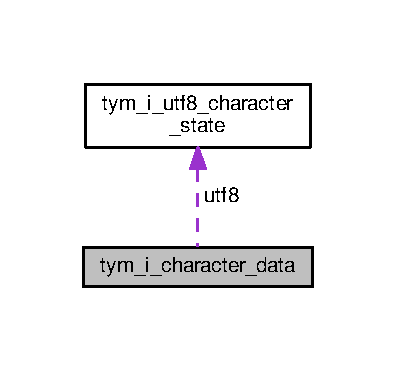
\includegraphics[width=190pt]{uniontym__i__character__data__coll__graph}
\end{center}
\end{figure}
\subsection*{Data Fields}
\begin{DoxyCompactItemize}
\item 
struct \hyperlink{structtym__i__utf8__character__state}{tym\+\_\+i\+\_\+utf8\+\_\+character\+\_\+state} \hyperlink{uniontym__i__character__data_ad0a8e001d32643615c5265e9af3b9079}{utf8}
\item 
char \hyperlink{uniontym__i__character__data_a128f7b66e5071854606106ee3801fafb}{byte}
\end{DoxyCompactItemize}


\subsection{Detailed Description}


Definition at line 113 of file pane.\+h.



\subsection{Field Documentation}
\mbox{\Hypertarget{uniontym__i__character__data_a128f7b66e5071854606106ee3801fafb}\label{uniontym__i__character__data_a128f7b66e5071854606106ee3801fafb}} 
\index{tym\+\_\+i\+\_\+character\+\_\+data@{tym\+\_\+i\+\_\+character\+\_\+data}!byte@{byte}}
\index{byte@{byte}!tym\+\_\+i\+\_\+character\+\_\+data@{tym\+\_\+i\+\_\+character\+\_\+data}}
\subsubsection{\texorpdfstring{byte}{byte}}
{\footnotesize\ttfamily char tym\+\_\+i\+\_\+character\+\_\+data\+::byte}



Definition at line 115 of file pane.\+h.

\mbox{\Hypertarget{uniontym__i__character__data_ad0a8e001d32643615c5265e9af3b9079}\label{uniontym__i__character__data_ad0a8e001d32643615c5265e9af3b9079}} 
\index{tym\+\_\+i\+\_\+character\+\_\+data@{tym\+\_\+i\+\_\+character\+\_\+data}!utf8@{utf8}}
\index{utf8@{utf8}!tym\+\_\+i\+\_\+character\+\_\+data@{tym\+\_\+i\+\_\+character\+\_\+data}}
\subsubsection{\texorpdfstring{utf8}{utf8}}
{\footnotesize\ttfamily struct \hyperlink{structtym__i__utf8__character__state}{tym\+\_\+i\+\_\+utf8\+\_\+character\+\_\+state} tym\+\_\+i\+\_\+character\+\_\+data\+::utf8}



Definition at line 114 of file pane.\+h.



The documentation for this union was generated from the following file\+:\begin{DoxyCompactItemize}
\item 
include/internal/\hyperlink{pane_8h}{pane.\+h}\end{DoxyCompactItemize}

\hypertarget{structtym__i__character__format}{}\section{tym\+\_\+i\+\_\+character\+\_\+format Struct Reference}
\label{structtym__i__character__format}\index{tym\+\_\+i\+\_\+character\+\_\+format@{tym\+\_\+i\+\_\+character\+\_\+format}}


{\ttfamily \#include $<$pane.\+h$>$}



Collaboration diagram for tym\+\_\+i\+\_\+character\+\_\+format\+:
\nopagebreak
\begin{figure}[H]
\begin{center}
\leavevmode
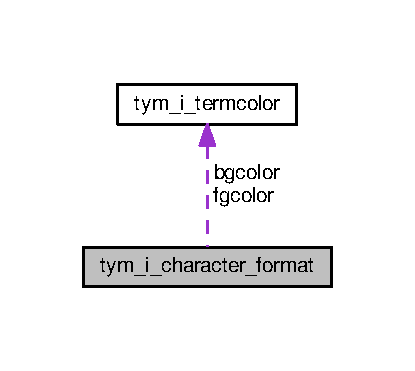
\includegraphics[width=199pt]{structtym__i__character__format__coll__graph}
\end{center}
\end{figure}
\subsection*{Data Fields}
\begin{DoxyCompactItemize}
\item 
enum \hyperlink{pane_8h_ac6609b89967e8b2b9e46a1630a260654}{tym\+\_\+i\+\_\+character\+\_\+attribute} \hyperlink{structtym__i__character__format_a276bf9587b4bdad1f8a3c0cefe42e9ae}{attribute}
\item 
struct \hyperlink{structtym__i__termcolor}{tym\+\_\+i\+\_\+termcolor} \hyperlink{structtym__i__character__format_acf1b3f3b19b6807936d8cc633b8fdb0e}{fgcolor}
\item 
struct \hyperlink{structtym__i__termcolor}{tym\+\_\+i\+\_\+termcolor} \hyperlink{structtym__i__character__format_afa091652fea5f7d0729d18fb4a8f984f}{bgcolor}
\end{DoxyCompactItemize}


\subsection{Detailed Description}


Definition at line 103 of file pane.\+h.



\subsection{Field Documentation}
\mbox{\Hypertarget{structtym__i__character__format_a276bf9587b4bdad1f8a3c0cefe42e9ae}\label{structtym__i__character__format_a276bf9587b4bdad1f8a3c0cefe42e9ae}} 
\index{tym\+\_\+i\+\_\+character\+\_\+format@{tym\+\_\+i\+\_\+character\+\_\+format}!attribute@{attribute}}
\index{attribute@{attribute}!tym\+\_\+i\+\_\+character\+\_\+format@{tym\+\_\+i\+\_\+character\+\_\+format}}
\subsubsection{\texorpdfstring{attribute}{attribute}}
{\footnotesize\ttfamily enum \hyperlink{pane_8h_ac6609b89967e8b2b9e46a1630a260654}{tym\+\_\+i\+\_\+character\+\_\+attribute} tym\+\_\+i\+\_\+character\+\_\+format\+::attribute}



Definition at line 104 of file pane.\+h.

\mbox{\Hypertarget{structtym__i__character__format_afa091652fea5f7d0729d18fb4a8f984f}\label{structtym__i__character__format_afa091652fea5f7d0729d18fb4a8f984f}} 
\index{tym\+\_\+i\+\_\+character\+\_\+format@{tym\+\_\+i\+\_\+character\+\_\+format}!bgcolor@{bgcolor}}
\index{bgcolor@{bgcolor}!tym\+\_\+i\+\_\+character\+\_\+format@{tym\+\_\+i\+\_\+character\+\_\+format}}
\subsubsection{\texorpdfstring{bgcolor}{bgcolor}}
{\footnotesize\ttfamily struct \hyperlink{structtym__i__termcolor}{tym\+\_\+i\+\_\+termcolor} tym\+\_\+i\+\_\+character\+\_\+format\+::bgcolor}



Definition at line 106 of file pane.\+h.

\mbox{\Hypertarget{structtym__i__character__format_acf1b3f3b19b6807936d8cc633b8fdb0e}\label{structtym__i__character__format_acf1b3f3b19b6807936d8cc633b8fdb0e}} 
\index{tym\+\_\+i\+\_\+character\+\_\+format@{tym\+\_\+i\+\_\+character\+\_\+format}!fgcolor@{fgcolor}}
\index{fgcolor@{fgcolor}!tym\+\_\+i\+\_\+character\+\_\+format@{tym\+\_\+i\+\_\+character\+\_\+format}}
\subsubsection{\texorpdfstring{fgcolor}{fgcolor}}
{\footnotesize\ttfamily struct \hyperlink{structtym__i__termcolor}{tym\+\_\+i\+\_\+termcolor} tym\+\_\+i\+\_\+character\+\_\+format\+::fgcolor}



Definition at line 105 of file pane.\+h.



The documentation for this struct was generated from the following file\+:\begin{DoxyCompactItemize}
\item 
include/internal/\hyperlink{pane_8h}{pane.\+h}\end{DoxyCompactItemize}

\hypertarget{structtym__i__command__sequence}{}\section{tym\+\_\+i\+\_\+command\+\_\+sequence Struct Reference}
\label{structtym__i__command__sequence}\index{tym\+\_\+i\+\_\+command\+\_\+sequence@{tym\+\_\+i\+\_\+command\+\_\+sequence}}


{\ttfamily \#include $<$parser.\+h$>$}



Collaboration diagram for tym\+\_\+i\+\_\+command\+\_\+sequence\+:
\nopagebreak
\begin{figure}[H]
\begin{center}
\leavevmode
\includegraphics[width=350pt]{structtym__i__command__sequence__coll__graph}
\end{center}
\end{figure}
\subsection*{Data Fields}
\begin{DoxyCompactItemize}
\item 
const char $\ast$ \hyperlink{structtym__i__command__sequence_a97eb218996497c02f77662293e3a617c}{sequence}
\item 
unsigned short \hyperlink{structtym__i__command__sequence_a26469eac6daf5799c118900e051c8def}{length}
\item 
const char $\ast$ \hyperlink{structtym__i__command__sequence_ac75a4e69eaf4c215b60f5d9d088f0583}{callback\+\_\+name}
\item 
\hyperlink{parser_8h_a647b0f7eb717ad806b441ebfdad60e30}{tym\+\_\+i\+\_\+csq\+\_\+sequence\+\_\+callback} \hyperlink{structtym__i__command__sequence_ae01318864f1edc1d61a6bed1e73773fa}{callback}
\end{DoxyCompactItemize}


\subsection{Detailed Description}


Definition at line 37 of file parser.\+h.



\subsection{Field Documentation}
\mbox{\Hypertarget{structtym__i__command__sequence_ae01318864f1edc1d61a6bed1e73773fa}\label{structtym__i__command__sequence_ae01318864f1edc1d61a6bed1e73773fa}} 
\index{tym\+\_\+i\+\_\+command\+\_\+sequence@{tym\+\_\+i\+\_\+command\+\_\+sequence}!callback@{callback}}
\index{callback@{callback}!tym\+\_\+i\+\_\+command\+\_\+sequence@{tym\+\_\+i\+\_\+command\+\_\+sequence}}
\subsubsection{\texorpdfstring{callback}{callback}}
{\footnotesize\ttfamily \hyperlink{parser_8h_a647b0f7eb717ad806b441ebfdad60e30}{tym\+\_\+i\+\_\+csq\+\_\+sequence\+\_\+callback} tym\+\_\+i\+\_\+command\+\_\+sequence\+::callback}



Definition at line 41 of file parser.\+h.

\mbox{\Hypertarget{structtym__i__command__sequence_ac75a4e69eaf4c215b60f5d9d088f0583}\label{structtym__i__command__sequence_ac75a4e69eaf4c215b60f5d9d088f0583}} 
\index{tym\+\_\+i\+\_\+command\+\_\+sequence@{tym\+\_\+i\+\_\+command\+\_\+sequence}!callback\+\_\+name@{callback\+\_\+name}}
\index{callback\+\_\+name@{callback\+\_\+name}!tym\+\_\+i\+\_\+command\+\_\+sequence@{tym\+\_\+i\+\_\+command\+\_\+sequence}}
\subsubsection{\texorpdfstring{callback\+\_\+name}{callback\_name}}
{\footnotesize\ttfamily const char$\ast$ tym\+\_\+i\+\_\+command\+\_\+sequence\+::callback\+\_\+name}



Definition at line 40 of file parser.\+h.

\mbox{\Hypertarget{structtym__i__command__sequence_a26469eac6daf5799c118900e051c8def}\label{structtym__i__command__sequence_a26469eac6daf5799c118900e051c8def}} 
\index{tym\+\_\+i\+\_\+command\+\_\+sequence@{tym\+\_\+i\+\_\+command\+\_\+sequence}!length@{length}}
\index{length@{length}!tym\+\_\+i\+\_\+command\+\_\+sequence@{tym\+\_\+i\+\_\+command\+\_\+sequence}}
\subsubsection{\texorpdfstring{length}{length}}
{\footnotesize\ttfamily unsigned short tym\+\_\+i\+\_\+command\+\_\+sequence\+::length}



Definition at line 39 of file parser.\+h.

\mbox{\Hypertarget{structtym__i__command__sequence_a97eb218996497c02f77662293e3a617c}\label{structtym__i__command__sequence_a97eb218996497c02f77662293e3a617c}} 
\index{tym\+\_\+i\+\_\+command\+\_\+sequence@{tym\+\_\+i\+\_\+command\+\_\+sequence}!sequence@{sequence}}
\index{sequence@{sequence}!tym\+\_\+i\+\_\+command\+\_\+sequence@{tym\+\_\+i\+\_\+command\+\_\+sequence}}
\subsubsection{\texorpdfstring{sequence}{sequence}}
{\footnotesize\ttfamily const char$\ast$ tym\+\_\+i\+\_\+command\+\_\+sequence\+::sequence}



Definition at line 38 of file parser.\+h.



The documentation for this struct was generated from the following file\+:\begin{DoxyCompactItemize}
\item 
include/internal/\hyperlink{parser_8h}{parser.\+h}\end{DoxyCompactItemize}

\hypertarget{structtym__i__handler__ptr__pair}{}\section{tym\+\_\+i\+\_\+handler\+\_\+ptr\+\_\+pair Struct Reference}
\label{structtym__i__handler__ptr__pair}\index{tym\+\_\+i\+\_\+handler\+\_\+ptr\+\_\+pair@{tym\+\_\+i\+\_\+handler\+\_\+ptr\+\_\+pair}}


{\ttfamily \#include $<$pane.\+h$>$}



Collaboration diagram for tym\+\_\+i\+\_\+handler\+\_\+ptr\+\_\+pair\+:
\nopagebreak
\begin{figure}[H]
\begin{center}
\leavevmode
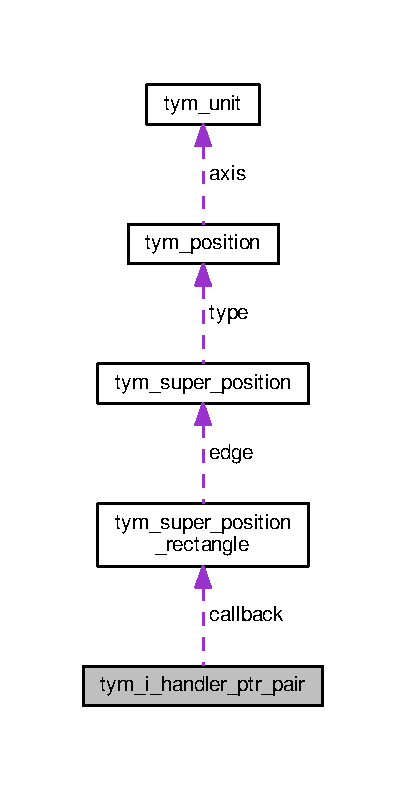
\includegraphics[width=195pt]{structtym__i__handler__ptr__pair__coll__graph}
\end{center}
\end{figure}
\subsection*{Data Fields}
\begin{DoxyCompactItemize}
\item 
void $\ast$ \hyperlink{structtym__i__handler__ptr__pair_a9cc2f422ffb3ed953f009d03ca5477bb}{ptr}
\item 
\hyperlink{libttymultiplex_8h_a7b785cb846faa92e5f2f5fbf32bdcde4}{tym\+\_\+resize\+\_\+handler\+\_\+t} \hyperlink{structtym__i__handler__ptr__pair_a2e8f24a33817fd8af89b9279f252fc8d}{callback}
\end{DoxyCompactItemize}


\subsection{Detailed Description}


Definition at line 16 of file pane.\+h.



\subsection{Field Documentation}
\mbox{\Hypertarget{structtym__i__handler__ptr__pair_a2e8f24a33817fd8af89b9279f252fc8d}\label{structtym__i__handler__ptr__pair_a2e8f24a33817fd8af89b9279f252fc8d}} 
\index{tym\+\_\+i\+\_\+handler\+\_\+ptr\+\_\+pair@{tym\+\_\+i\+\_\+handler\+\_\+ptr\+\_\+pair}!callback@{callback}}
\index{callback@{callback}!tym\+\_\+i\+\_\+handler\+\_\+ptr\+\_\+pair@{tym\+\_\+i\+\_\+handler\+\_\+ptr\+\_\+pair}}
\subsubsection{\texorpdfstring{callback}{callback}}
{\footnotesize\ttfamily \hyperlink{libttymultiplex_8h_a7b785cb846faa92e5f2f5fbf32bdcde4}{tym\+\_\+resize\+\_\+handler\+\_\+t} tym\+\_\+i\+\_\+handler\+\_\+ptr\+\_\+pair\+::callback}



Definition at line 18 of file pane.\+h.

\mbox{\Hypertarget{structtym__i__handler__ptr__pair_a9cc2f422ffb3ed953f009d03ca5477bb}\label{structtym__i__handler__ptr__pair_a9cc2f422ffb3ed953f009d03ca5477bb}} 
\index{tym\+\_\+i\+\_\+handler\+\_\+ptr\+\_\+pair@{tym\+\_\+i\+\_\+handler\+\_\+ptr\+\_\+pair}!ptr@{ptr}}
\index{ptr@{ptr}!tym\+\_\+i\+\_\+handler\+\_\+ptr\+\_\+pair@{tym\+\_\+i\+\_\+handler\+\_\+ptr\+\_\+pair}}
\subsubsection{\texorpdfstring{ptr}{ptr}}
{\footnotesize\ttfamily void$\ast$ tym\+\_\+i\+\_\+handler\+\_\+ptr\+\_\+pair\+::ptr}



Definition at line 17 of file pane.\+h.



The documentation for this struct was generated from the following file\+:\begin{DoxyCompactItemize}
\item 
include/internal/\hyperlink{pane_8h}{pane.\+h}\end{DoxyCompactItemize}

\hypertarget{structtym__i__pane__internal}{}\section{tym\+\_\+i\+\_\+pane\+\_\+internal Struct Reference}
\label{structtym__i__pane__internal}\index{tym\+\_\+i\+\_\+pane\+\_\+internal@{tym\+\_\+i\+\_\+pane\+\_\+internal}}


{\ttfamily \#include $<$pane.\+h$>$}



Collaboration diagram for tym\+\_\+i\+\_\+pane\+\_\+internal\+:
\nopagebreak
\begin{figure}[H]
\begin{center}
\leavevmode
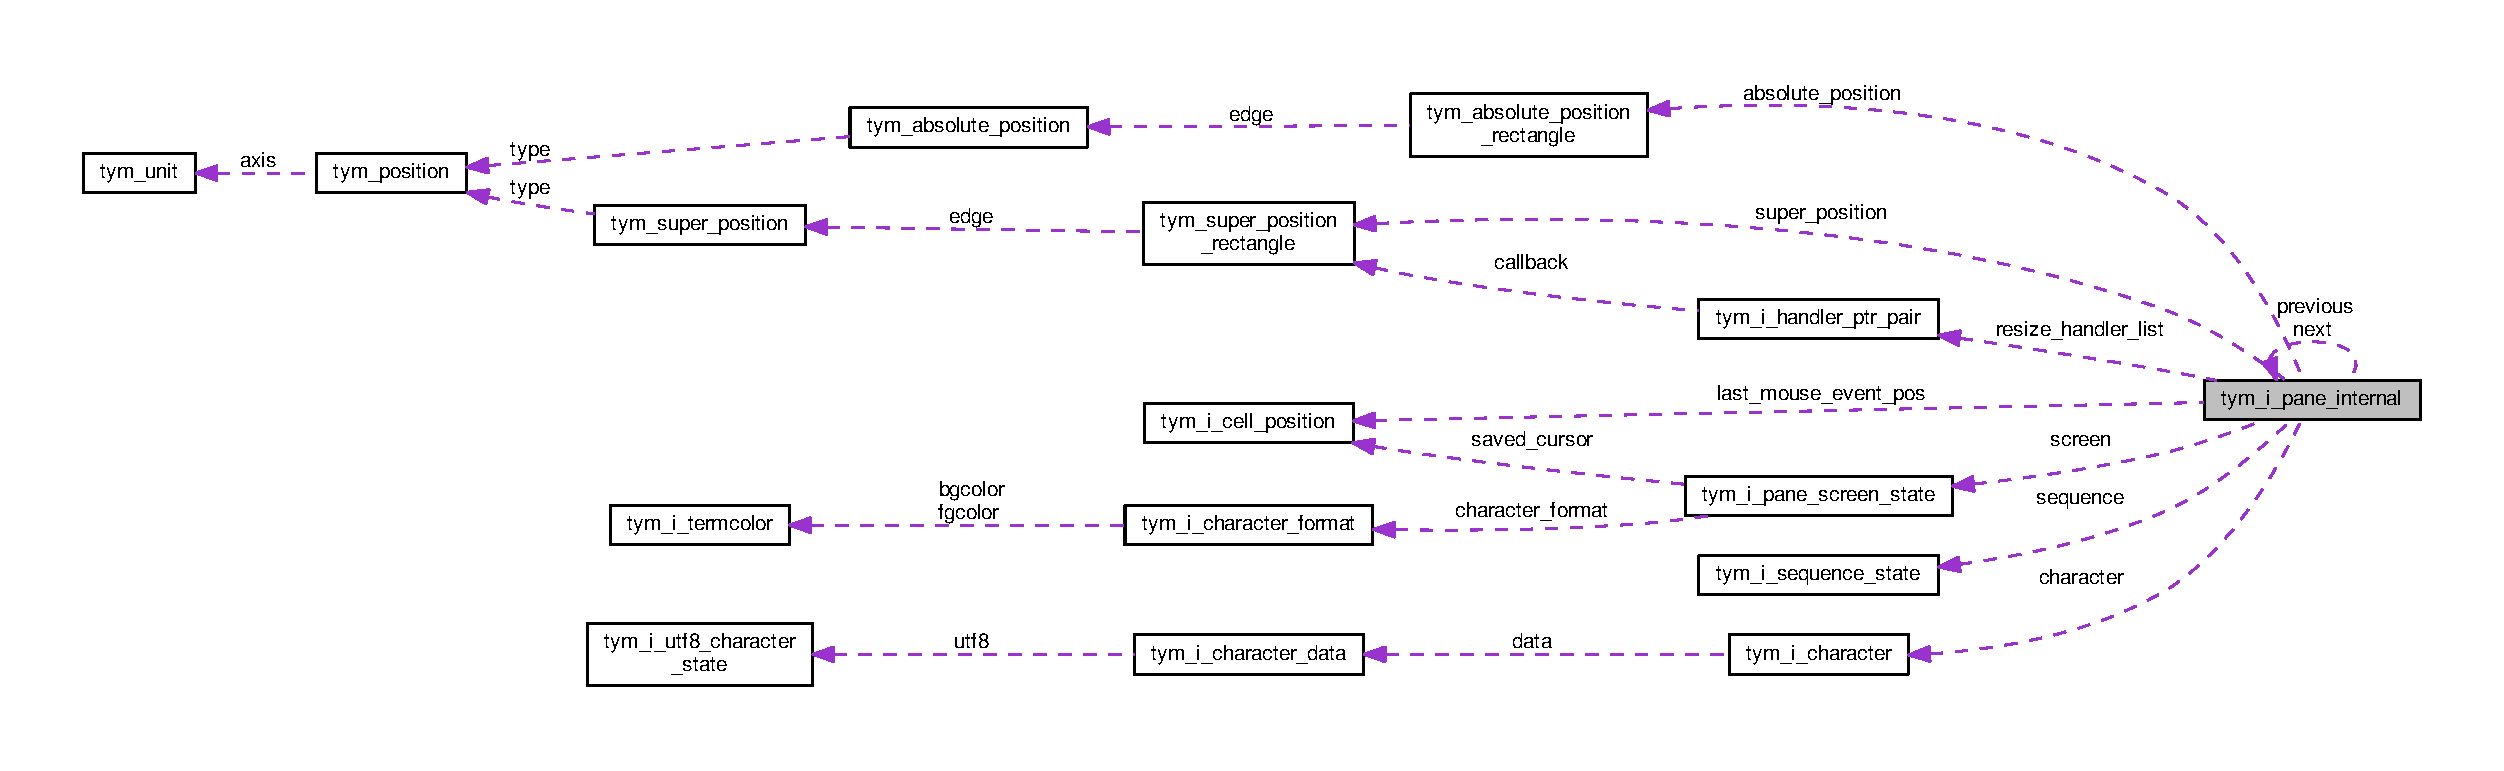
\includegraphics[width=350pt]{structtym__i__pane__internal__coll__graph}
\end{center}
\end{figure}
\subsection*{Data Fields}
\begin{DoxyCompactItemize}
\item 
struct \hyperlink{structtym__i__pane__internal}{tym\+\_\+i\+\_\+pane\+\_\+internal} $\ast$ \hyperlink{structtym__i__pane__internal_a922aa2239bb2f3d008bc35a3caddb8c3}{previous}
\item 
struct \hyperlink{structtym__i__pane__internal}{tym\+\_\+i\+\_\+pane\+\_\+internal} $\ast$ \hyperlink{structtym__i__pane__internal_a6a0cdccfe24cb9b09ae1754cf9d4c029}{next}
\item 
int \hyperlink{structtym__i__pane__internal_a17e1f7d06c7214ae1ad4912370dcc4a1}{id}
\item 
int \hyperlink{structtym__i__pane__internal_ae32841ea8e94f488eac503995206380b}{master}
\item 
int \hyperlink{structtym__i__pane__internal_aae38651ca650725201ea0e4a7ac5e893}{slave}
\item 
bool \hyperlink{structtym__i__pane__internal_ad10df02effe8dee789bf80a8a6f85b41}{nofocus}
\item 
void $\ast$ \hyperlink{structtym__i__pane__internal_af6a6ae990267090f21c804525a89128a}{backend}
\item 
struct \hyperlink{structtym__i__sequence__state}{tym\+\_\+i\+\_\+sequence\+\_\+state} \hyperlink{structtym__i__pane__internal_acee6942f5fc8a08292cdacf9f50fcf6e}{sequence}
\item 
struct termios \hyperlink{structtym__i__pane__internal_a4d03c0c97686307362307fd44c3edd50}{termios}
\item 
struct \hyperlink{structtym__super__position__rectangle}{tym\+\_\+super\+\_\+position\+\_\+rectangle} \hyperlink{structtym__i__pane__internal_a6130559b5f02e294f71981c51535fd06}{super\+\_\+position}
\item 
struct \hyperlink{structtym__absolute__position__rectangle}{tym\+\_\+absolute\+\_\+position\+\_\+rectangle} \hyperlink{structtym__i__pane__internal_a05be638aab84faf85b300b6021b772d8}{absolute\+\_\+position}
\item 
size\+\_\+t \hyperlink{structtym__i__pane__internal_a084a6b169726095a350eddddbdd78c65}{resize\+\_\+handler\+\_\+count}
\item 
struct \hyperlink{structtym__i__handler__ptr__pair}{tym\+\_\+i\+\_\+handler\+\_\+ptr\+\_\+pair} $\ast$ \hyperlink{structtym__i__pane__internal_a563a81b01e867376d388aa77061c1ca8}{resize\+\_\+handler\+\_\+list}
\item 
struct \hyperlink{structtym__i__character}{tym\+\_\+i\+\_\+character} \hyperlink{structtym__i__pane__internal_a019ad181f81cb30eca1396c630b6e4be}{character}
\item 
enum \hyperlink{pane_8h_a49f1d9b192f4f01ff444123abde24761}{tym\+\_\+i\+\_\+pane\+\_\+screen} \hyperlink{structtym__i__pane__internal_a7ec548dbe248ba7f654569127819dc3c}{current\+\_\+screen}
\item 
struct \hyperlink{structtym__i__cell__position}{tym\+\_\+i\+\_\+cell\+\_\+position} \hyperlink{structtym__i__pane__internal_a89ad2bf59a75b2813352bc070e039f04}{last\+\_\+mouse\+\_\+event\+\_\+pos}
\item 
enum \hyperlink{libttymultiplex_8h_a9223cca7368df5ee528dec0bfa0c3ab3}{tym\+\_\+button} \hyperlink{structtym__i__pane__internal_adaeb64342d1a99fa26110a0f41993326}{last\+\_\+button}
\item 
enum \hyperlink{pane_8h_a271f5b51a492d1598aad17ccd8ebd0c4}{mouse\+\_\+mode} \hyperlink{structtym__i__pane__internal_a55eb70f7a40f96f3348dc1690e9c53c2}{mouse\+\_\+mode}
\item 
struct \hyperlink{structtym__i__pane__screen__state}{tym\+\_\+i\+\_\+pane\+\_\+screen\+\_\+state} \hyperlink{structtym__i__pane__internal_a169132da2187f1791ae9252c63b7321a}{screen} \mbox{[}\hyperlink{pane_8h_a49f1d9b192f4f01ff444123abde24761a4675b455ce9ebdc1c317e91e0c66e5e0}{T\+Y\+M\+\_\+\+I\+\_\+\+S\+C\+R\+E\+E\+N\+\_\+\+C\+O\+U\+NT}\mbox{]}
\end{DoxyCompactItemize}


\subsection{Detailed Description}


Definition at line 136 of file pane.\+h.



\subsection{Field Documentation}
\mbox{\Hypertarget{structtym__i__pane__internal_a05be638aab84faf85b300b6021b772d8}\label{structtym__i__pane__internal_a05be638aab84faf85b300b6021b772d8}} 
\index{tym\+\_\+i\+\_\+pane\+\_\+internal@{tym\+\_\+i\+\_\+pane\+\_\+internal}!absolute\+\_\+position@{absolute\+\_\+position}}
\index{absolute\+\_\+position@{absolute\+\_\+position}!tym\+\_\+i\+\_\+pane\+\_\+internal@{tym\+\_\+i\+\_\+pane\+\_\+internal}}
\subsubsection{\texorpdfstring{absolute\+\_\+position}{absolute\_position}}
{\footnotesize\ttfamily struct \hyperlink{structtym__absolute__position__rectangle}{tym\+\_\+absolute\+\_\+position\+\_\+rectangle} tym\+\_\+i\+\_\+pane\+\_\+internal\+::absolute\+\_\+position}



Definition at line 145 of file pane.\+h.

\mbox{\Hypertarget{structtym__i__pane__internal_af6a6ae990267090f21c804525a89128a}\label{structtym__i__pane__internal_af6a6ae990267090f21c804525a89128a}} 
\index{tym\+\_\+i\+\_\+pane\+\_\+internal@{tym\+\_\+i\+\_\+pane\+\_\+internal}!backend@{backend}}
\index{backend@{backend}!tym\+\_\+i\+\_\+pane\+\_\+internal@{tym\+\_\+i\+\_\+pane\+\_\+internal}}
\subsubsection{\texorpdfstring{backend}{backend}}
{\footnotesize\ttfamily void$\ast$ tym\+\_\+i\+\_\+pane\+\_\+internal\+::backend}



Definition at line 141 of file pane.\+h.

\mbox{\Hypertarget{structtym__i__pane__internal_a019ad181f81cb30eca1396c630b6e4be}\label{structtym__i__pane__internal_a019ad181f81cb30eca1396c630b6e4be}} 
\index{tym\+\_\+i\+\_\+pane\+\_\+internal@{tym\+\_\+i\+\_\+pane\+\_\+internal}!character@{character}}
\index{character@{character}!tym\+\_\+i\+\_\+pane\+\_\+internal@{tym\+\_\+i\+\_\+pane\+\_\+internal}}
\subsubsection{\texorpdfstring{character}{character}}
{\footnotesize\ttfamily struct \hyperlink{structtym__i__character}{tym\+\_\+i\+\_\+character} tym\+\_\+i\+\_\+pane\+\_\+internal\+::character}



Definition at line 149 of file pane.\+h.

\mbox{\Hypertarget{structtym__i__pane__internal_a7ec548dbe248ba7f654569127819dc3c}\label{structtym__i__pane__internal_a7ec548dbe248ba7f654569127819dc3c}} 
\index{tym\+\_\+i\+\_\+pane\+\_\+internal@{tym\+\_\+i\+\_\+pane\+\_\+internal}!current\+\_\+screen@{current\+\_\+screen}}
\index{current\+\_\+screen@{current\+\_\+screen}!tym\+\_\+i\+\_\+pane\+\_\+internal@{tym\+\_\+i\+\_\+pane\+\_\+internal}}
\subsubsection{\texorpdfstring{current\+\_\+screen}{current\_screen}}
{\footnotesize\ttfamily enum \hyperlink{pane_8h_a49f1d9b192f4f01ff444123abde24761}{tym\+\_\+i\+\_\+pane\+\_\+screen} tym\+\_\+i\+\_\+pane\+\_\+internal\+::current\+\_\+screen}



Definition at line 150 of file pane.\+h.

\mbox{\Hypertarget{structtym__i__pane__internal_a17e1f7d06c7214ae1ad4912370dcc4a1}\label{structtym__i__pane__internal_a17e1f7d06c7214ae1ad4912370dcc4a1}} 
\index{tym\+\_\+i\+\_\+pane\+\_\+internal@{tym\+\_\+i\+\_\+pane\+\_\+internal}!id@{id}}
\index{id@{id}!tym\+\_\+i\+\_\+pane\+\_\+internal@{tym\+\_\+i\+\_\+pane\+\_\+internal}}
\subsubsection{\texorpdfstring{id}{id}}
{\footnotesize\ttfamily int tym\+\_\+i\+\_\+pane\+\_\+internal\+::id}



Definition at line 138 of file pane.\+h.

\mbox{\Hypertarget{structtym__i__pane__internal_adaeb64342d1a99fa26110a0f41993326}\label{structtym__i__pane__internal_adaeb64342d1a99fa26110a0f41993326}} 
\index{tym\+\_\+i\+\_\+pane\+\_\+internal@{tym\+\_\+i\+\_\+pane\+\_\+internal}!last\+\_\+button@{last\+\_\+button}}
\index{last\+\_\+button@{last\+\_\+button}!tym\+\_\+i\+\_\+pane\+\_\+internal@{tym\+\_\+i\+\_\+pane\+\_\+internal}}
\subsubsection{\texorpdfstring{last\+\_\+button}{last\_button}}
{\footnotesize\ttfamily enum \hyperlink{libttymultiplex_8h_a9223cca7368df5ee528dec0bfa0c3ab3}{tym\+\_\+button} tym\+\_\+i\+\_\+pane\+\_\+internal\+::last\+\_\+button}



Definition at line 152 of file pane.\+h.

\mbox{\Hypertarget{structtym__i__pane__internal_a89ad2bf59a75b2813352bc070e039f04}\label{structtym__i__pane__internal_a89ad2bf59a75b2813352bc070e039f04}} 
\index{tym\+\_\+i\+\_\+pane\+\_\+internal@{tym\+\_\+i\+\_\+pane\+\_\+internal}!last\+\_\+mouse\+\_\+event\+\_\+pos@{last\+\_\+mouse\+\_\+event\+\_\+pos}}
\index{last\+\_\+mouse\+\_\+event\+\_\+pos@{last\+\_\+mouse\+\_\+event\+\_\+pos}!tym\+\_\+i\+\_\+pane\+\_\+internal@{tym\+\_\+i\+\_\+pane\+\_\+internal}}
\subsubsection{\texorpdfstring{last\+\_\+mouse\+\_\+event\+\_\+pos}{last\_mouse\_event\_pos}}
{\footnotesize\ttfamily struct \hyperlink{structtym__i__cell__position}{tym\+\_\+i\+\_\+cell\+\_\+position} tym\+\_\+i\+\_\+pane\+\_\+internal\+::last\+\_\+mouse\+\_\+event\+\_\+pos}



Definition at line 151 of file pane.\+h.

\mbox{\Hypertarget{structtym__i__pane__internal_ae32841ea8e94f488eac503995206380b}\label{structtym__i__pane__internal_ae32841ea8e94f488eac503995206380b}} 
\index{tym\+\_\+i\+\_\+pane\+\_\+internal@{tym\+\_\+i\+\_\+pane\+\_\+internal}!master@{master}}
\index{master@{master}!tym\+\_\+i\+\_\+pane\+\_\+internal@{tym\+\_\+i\+\_\+pane\+\_\+internal}}
\subsubsection{\texorpdfstring{master}{master}}
{\footnotesize\ttfamily int tym\+\_\+i\+\_\+pane\+\_\+internal\+::master}



Definition at line 139 of file pane.\+h.

\mbox{\Hypertarget{structtym__i__pane__internal_a55eb70f7a40f96f3348dc1690e9c53c2}\label{structtym__i__pane__internal_a55eb70f7a40f96f3348dc1690e9c53c2}} 
\index{tym\+\_\+i\+\_\+pane\+\_\+internal@{tym\+\_\+i\+\_\+pane\+\_\+internal}!mouse\+\_\+mode@{mouse\+\_\+mode}}
\index{mouse\+\_\+mode@{mouse\+\_\+mode}!tym\+\_\+i\+\_\+pane\+\_\+internal@{tym\+\_\+i\+\_\+pane\+\_\+internal}}
\subsubsection{\texorpdfstring{mouse\+\_\+mode}{mouse\_mode}}
{\footnotesize\ttfamily enum \hyperlink{pane_8h_a271f5b51a492d1598aad17ccd8ebd0c4}{mouse\+\_\+mode} tym\+\_\+i\+\_\+pane\+\_\+internal\+::mouse\+\_\+mode}



Definition at line 153 of file pane.\+h.

\mbox{\Hypertarget{structtym__i__pane__internal_a6a0cdccfe24cb9b09ae1754cf9d4c029}\label{structtym__i__pane__internal_a6a0cdccfe24cb9b09ae1754cf9d4c029}} 
\index{tym\+\_\+i\+\_\+pane\+\_\+internal@{tym\+\_\+i\+\_\+pane\+\_\+internal}!next@{next}}
\index{next@{next}!tym\+\_\+i\+\_\+pane\+\_\+internal@{tym\+\_\+i\+\_\+pane\+\_\+internal}}
\subsubsection{\texorpdfstring{next}{next}}
{\footnotesize\ttfamily struct \hyperlink{structtym__i__pane__internal}{tym\+\_\+i\+\_\+pane\+\_\+internal} $\ast$ tym\+\_\+i\+\_\+pane\+\_\+internal\+::next}



Definition at line 137 of file pane.\+h.

\mbox{\Hypertarget{structtym__i__pane__internal_ad10df02effe8dee789bf80a8a6f85b41}\label{structtym__i__pane__internal_ad10df02effe8dee789bf80a8a6f85b41}} 
\index{tym\+\_\+i\+\_\+pane\+\_\+internal@{tym\+\_\+i\+\_\+pane\+\_\+internal}!nofocus@{nofocus}}
\index{nofocus@{nofocus}!tym\+\_\+i\+\_\+pane\+\_\+internal@{tym\+\_\+i\+\_\+pane\+\_\+internal}}
\subsubsection{\texorpdfstring{nofocus}{nofocus}}
{\footnotesize\ttfamily bool tym\+\_\+i\+\_\+pane\+\_\+internal\+::nofocus}



Definition at line 140 of file pane.\+h.

\mbox{\Hypertarget{structtym__i__pane__internal_a922aa2239bb2f3d008bc35a3caddb8c3}\label{structtym__i__pane__internal_a922aa2239bb2f3d008bc35a3caddb8c3}} 
\index{tym\+\_\+i\+\_\+pane\+\_\+internal@{tym\+\_\+i\+\_\+pane\+\_\+internal}!previous@{previous}}
\index{previous@{previous}!tym\+\_\+i\+\_\+pane\+\_\+internal@{tym\+\_\+i\+\_\+pane\+\_\+internal}}
\subsubsection{\texorpdfstring{previous}{previous}}
{\footnotesize\ttfamily struct \hyperlink{structtym__i__pane__internal}{tym\+\_\+i\+\_\+pane\+\_\+internal}$\ast$ tym\+\_\+i\+\_\+pane\+\_\+internal\+::previous}



Definition at line 137 of file pane.\+h.

\mbox{\Hypertarget{structtym__i__pane__internal_a084a6b169726095a350eddddbdd78c65}\label{structtym__i__pane__internal_a084a6b169726095a350eddddbdd78c65}} 
\index{tym\+\_\+i\+\_\+pane\+\_\+internal@{tym\+\_\+i\+\_\+pane\+\_\+internal}!resize\+\_\+handler\+\_\+count@{resize\+\_\+handler\+\_\+count}}
\index{resize\+\_\+handler\+\_\+count@{resize\+\_\+handler\+\_\+count}!tym\+\_\+i\+\_\+pane\+\_\+internal@{tym\+\_\+i\+\_\+pane\+\_\+internal}}
\subsubsection{\texorpdfstring{resize\+\_\+handler\+\_\+count}{resize\_handler\_count}}
{\footnotesize\ttfamily size\+\_\+t tym\+\_\+i\+\_\+pane\+\_\+internal\+::resize\+\_\+handler\+\_\+count}



Definition at line 146 of file pane.\+h.

\mbox{\Hypertarget{structtym__i__pane__internal_a563a81b01e867376d388aa77061c1ca8}\label{structtym__i__pane__internal_a563a81b01e867376d388aa77061c1ca8}} 
\index{tym\+\_\+i\+\_\+pane\+\_\+internal@{tym\+\_\+i\+\_\+pane\+\_\+internal}!resize\+\_\+handler\+\_\+list@{resize\+\_\+handler\+\_\+list}}
\index{resize\+\_\+handler\+\_\+list@{resize\+\_\+handler\+\_\+list}!tym\+\_\+i\+\_\+pane\+\_\+internal@{tym\+\_\+i\+\_\+pane\+\_\+internal}}
\subsubsection{\texorpdfstring{resize\+\_\+handler\+\_\+list}{resize\_handler\_list}}
{\footnotesize\ttfamily struct \hyperlink{structtym__i__handler__ptr__pair}{tym\+\_\+i\+\_\+handler\+\_\+ptr\+\_\+pair}$\ast$ tym\+\_\+i\+\_\+pane\+\_\+internal\+::resize\+\_\+handler\+\_\+list}



Definition at line 147 of file pane.\+h.

\mbox{\Hypertarget{structtym__i__pane__internal_a169132da2187f1791ae9252c63b7321a}\label{structtym__i__pane__internal_a169132da2187f1791ae9252c63b7321a}} 
\index{tym\+\_\+i\+\_\+pane\+\_\+internal@{tym\+\_\+i\+\_\+pane\+\_\+internal}!screen@{screen}}
\index{screen@{screen}!tym\+\_\+i\+\_\+pane\+\_\+internal@{tym\+\_\+i\+\_\+pane\+\_\+internal}}
\subsubsection{\texorpdfstring{screen}{screen}}
{\footnotesize\ttfamily struct \hyperlink{structtym__i__pane__screen__state}{tym\+\_\+i\+\_\+pane\+\_\+screen\+\_\+state} tym\+\_\+i\+\_\+pane\+\_\+internal\+::screen\mbox{[}\hyperlink{pane_8h_a49f1d9b192f4f01ff444123abde24761a4675b455ce9ebdc1c317e91e0c66e5e0}{T\+Y\+M\+\_\+\+I\+\_\+\+S\+C\+R\+E\+E\+N\+\_\+\+C\+O\+U\+NT}\mbox{]}}



Definition at line 155 of file pane.\+h.

\mbox{\Hypertarget{structtym__i__pane__internal_acee6942f5fc8a08292cdacf9f50fcf6e}\label{structtym__i__pane__internal_acee6942f5fc8a08292cdacf9f50fcf6e}} 
\index{tym\+\_\+i\+\_\+pane\+\_\+internal@{tym\+\_\+i\+\_\+pane\+\_\+internal}!sequence@{sequence}}
\index{sequence@{sequence}!tym\+\_\+i\+\_\+pane\+\_\+internal@{tym\+\_\+i\+\_\+pane\+\_\+internal}}
\subsubsection{\texorpdfstring{sequence}{sequence}}
{\footnotesize\ttfamily struct \hyperlink{structtym__i__sequence__state}{tym\+\_\+i\+\_\+sequence\+\_\+state} tym\+\_\+i\+\_\+pane\+\_\+internal\+::sequence}



Definition at line 142 of file pane.\+h.

\mbox{\Hypertarget{structtym__i__pane__internal_aae38651ca650725201ea0e4a7ac5e893}\label{structtym__i__pane__internal_aae38651ca650725201ea0e4a7ac5e893}} 
\index{tym\+\_\+i\+\_\+pane\+\_\+internal@{tym\+\_\+i\+\_\+pane\+\_\+internal}!slave@{slave}}
\index{slave@{slave}!tym\+\_\+i\+\_\+pane\+\_\+internal@{tym\+\_\+i\+\_\+pane\+\_\+internal}}
\subsubsection{\texorpdfstring{slave}{slave}}
{\footnotesize\ttfamily int tym\+\_\+i\+\_\+pane\+\_\+internal\+::slave}



Definition at line 139 of file pane.\+h.

\mbox{\Hypertarget{structtym__i__pane__internal_a6130559b5f02e294f71981c51535fd06}\label{structtym__i__pane__internal_a6130559b5f02e294f71981c51535fd06}} 
\index{tym\+\_\+i\+\_\+pane\+\_\+internal@{tym\+\_\+i\+\_\+pane\+\_\+internal}!super\+\_\+position@{super\+\_\+position}}
\index{super\+\_\+position@{super\+\_\+position}!tym\+\_\+i\+\_\+pane\+\_\+internal@{tym\+\_\+i\+\_\+pane\+\_\+internal}}
\subsubsection{\texorpdfstring{super\+\_\+position}{super\_position}}
{\footnotesize\ttfamily struct \hyperlink{structtym__super__position__rectangle}{tym\+\_\+super\+\_\+position\+\_\+rectangle} tym\+\_\+i\+\_\+pane\+\_\+internal\+::super\+\_\+position}



Definition at line 144 of file pane.\+h.

\mbox{\Hypertarget{structtym__i__pane__internal_a4d03c0c97686307362307fd44c3edd50}\label{structtym__i__pane__internal_a4d03c0c97686307362307fd44c3edd50}} 
\index{tym\+\_\+i\+\_\+pane\+\_\+internal@{tym\+\_\+i\+\_\+pane\+\_\+internal}!termios@{termios}}
\index{termios@{termios}!tym\+\_\+i\+\_\+pane\+\_\+internal@{tym\+\_\+i\+\_\+pane\+\_\+internal}}
\subsubsection{\texorpdfstring{termios}{termios}}
{\footnotesize\ttfamily struct termios tym\+\_\+i\+\_\+pane\+\_\+internal\+::termios}



Definition at line 143 of file pane.\+h.



The documentation for this struct was generated from the following file\+:\begin{DoxyCompactItemize}
\item 
include/internal/\hyperlink{pane_8h}{pane.\+h}\end{DoxyCompactItemize}

\hypertarget{structtym__i__pane__screen__state}{}\section{tym\+\_\+i\+\_\+pane\+\_\+screen\+\_\+state Struct Reference}
\label{structtym__i__pane__screen__state}\index{tym\+\_\+i\+\_\+pane\+\_\+screen\+\_\+state@{tym\+\_\+i\+\_\+pane\+\_\+screen\+\_\+state}}


{\ttfamily \#include $<$pane.\+h$>$}



Collaboration diagram for tym\+\_\+i\+\_\+pane\+\_\+screen\+\_\+state\+:
\nopagebreak
\begin{figure}[H]
\begin{center}
\leavevmode
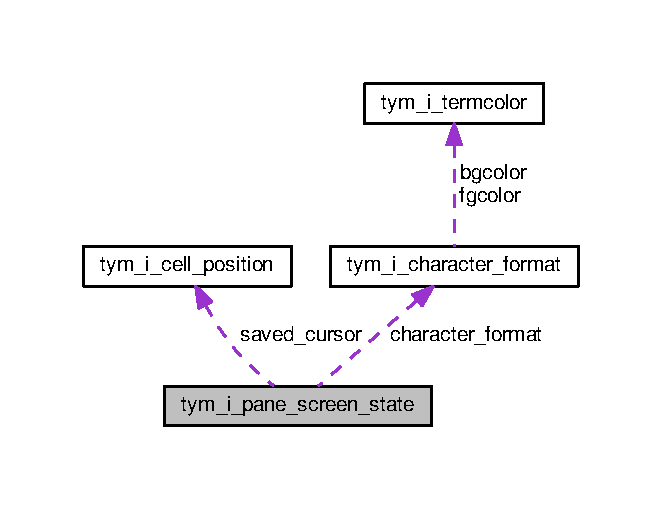
\includegraphics[width=318pt]{structtym__i__pane__screen__state__coll__graph}
\end{center}
\end{figure}
\subsection*{Data Fields}
\begin{DoxyCompactItemize}
\item 
struct \hyperlink{structtym__i__cell__position}{tym\+\_\+i\+\_\+cell\+\_\+position} cursor \hyperlink{structtym__i__pane__screen__state_aa67b24ce660b6da6aa9393b3f3acd61d}{saved\+\_\+cursor}
\item 
struct \hyperlink{structtym__i__character__format}{tym\+\_\+i\+\_\+character\+\_\+format} \hyperlink{structtym__i__pane__screen__state_a868cd2d97f372aacca0afaf7b42608e9}{character\+\_\+format}
\item 
enum \hyperlink{pane_8h_afec42adba111d829539aa660cfd36619}{tym\+\_\+i\+\_\+keypad\+\_\+mode} \hyperlink{structtym__i__pane__screen__state_a9373bd32028eb3b205d1381e8ff7e13e}{keypad\+\_\+mode}
\item 
enum \hyperlink{pane_8h_af72f527ead3cfb25d576d72dba239ba9}{tym\+\_\+i\+\_\+cursor\+\_\+key\+\_\+mode} \hyperlink{structtym__i__pane__screen__state_a884bae9505ac220fa9a09105bef0f0b2}{cursor\+\_\+key\+\_\+mode}
\item 
unsigned \hyperlink{structtym__i__pane__screen__state_af3665243e3d6dc3e117edc2cc4486144}{scroll\+\_\+region\+\_\+top}
\item 
unsigned \hyperlink{structtym__i__pane__screen__state_ad50d422fce8986b77b5a50267f7c9896}{scroll\+\_\+region\+\_\+bottom}
\item 
bool \hyperlink{structtym__i__pane__screen__state_a7170520b3f9887e5ba5726851ec3169e}{insert\+\_\+mode}\+: 1
\item 
bool \hyperlink{structtym__i__pane__screen__state_a1a02345aba0a0a93696e4892fcea3551}{origin\+\_\+mode}\+: 1
\item 
bool \hyperlink{structtym__i__pane__screen__state_aa47e037b07d6b0d8e14a32c9ad13dd0d}{wraparound\+\_\+mode\+\_\+off}\+: 1
\end{DoxyCompactItemize}


\subsection{Detailed Description}


Definition at line 125 of file pane.\+h.



\subsection{Field Documentation}
\mbox{\Hypertarget{structtym__i__pane__screen__state_a868cd2d97f372aacca0afaf7b42608e9}\label{structtym__i__pane__screen__state_a868cd2d97f372aacca0afaf7b42608e9}} 
\index{tym\+\_\+i\+\_\+pane\+\_\+screen\+\_\+state@{tym\+\_\+i\+\_\+pane\+\_\+screen\+\_\+state}!character\+\_\+format@{character\+\_\+format}}
\index{character\+\_\+format@{character\+\_\+format}!tym\+\_\+i\+\_\+pane\+\_\+screen\+\_\+state@{tym\+\_\+i\+\_\+pane\+\_\+screen\+\_\+state}}
\subsubsection{\texorpdfstring{character\+\_\+format}{character\_format}}
{\footnotesize\ttfamily struct \hyperlink{structtym__i__character__format}{tym\+\_\+i\+\_\+character\+\_\+format} tym\+\_\+i\+\_\+pane\+\_\+screen\+\_\+state\+::character\+\_\+format}



Definition at line 127 of file pane.\+h.

\mbox{\Hypertarget{structtym__i__pane__screen__state_a884bae9505ac220fa9a09105bef0f0b2}\label{structtym__i__pane__screen__state_a884bae9505ac220fa9a09105bef0f0b2}} 
\index{tym\+\_\+i\+\_\+pane\+\_\+screen\+\_\+state@{tym\+\_\+i\+\_\+pane\+\_\+screen\+\_\+state}!cursor\+\_\+key\+\_\+mode@{cursor\+\_\+key\+\_\+mode}}
\index{cursor\+\_\+key\+\_\+mode@{cursor\+\_\+key\+\_\+mode}!tym\+\_\+i\+\_\+pane\+\_\+screen\+\_\+state@{tym\+\_\+i\+\_\+pane\+\_\+screen\+\_\+state}}
\subsubsection{\texorpdfstring{cursor\+\_\+key\+\_\+mode}{cursor\_key\_mode}}
{\footnotesize\ttfamily enum \hyperlink{pane_8h_af72f527ead3cfb25d576d72dba239ba9}{tym\+\_\+i\+\_\+cursor\+\_\+key\+\_\+mode} tym\+\_\+i\+\_\+pane\+\_\+screen\+\_\+state\+::cursor\+\_\+key\+\_\+mode}



Definition at line 129 of file pane.\+h.

\mbox{\Hypertarget{structtym__i__pane__screen__state_a7170520b3f9887e5ba5726851ec3169e}\label{structtym__i__pane__screen__state_a7170520b3f9887e5ba5726851ec3169e}} 
\index{tym\+\_\+i\+\_\+pane\+\_\+screen\+\_\+state@{tym\+\_\+i\+\_\+pane\+\_\+screen\+\_\+state}!insert\+\_\+mode@{insert\+\_\+mode}}
\index{insert\+\_\+mode@{insert\+\_\+mode}!tym\+\_\+i\+\_\+pane\+\_\+screen\+\_\+state@{tym\+\_\+i\+\_\+pane\+\_\+screen\+\_\+state}}
\subsubsection{\texorpdfstring{insert\+\_\+mode}{insert\_mode}}
{\footnotesize\ttfamily bool tym\+\_\+i\+\_\+pane\+\_\+screen\+\_\+state\+::insert\+\_\+mode}



Definition at line 131 of file pane.\+h.

\mbox{\Hypertarget{structtym__i__pane__screen__state_a9373bd32028eb3b205d1381e8ff7e13e}\label{structtym__i__pane__screen__state_a9373bd32028eb3b205d1381e8ff7e13e}} 
\index{tym\+\_\+i\+\_\+pane\+\_\+screen\+\_\+state@{tym\+\_\+i\+\_\+pane\+\_\+screen\+\_\+state}!keypad\+\_\+mode@{keypad\+\_\+mode}}
\index{keypad\+\_\+mode@{keypad\+\_\+mode}!tym\+\_\+i\+\_\+pane\+\_\+screen\+\_\+state@{tym\+\_\+i\+\_\+pane\+\_\+screen\+\_\+state}}
\subsubsection{\texorpdfstring{keypad\+\_\+mode}{keypad\_mode}}
{\footnotesize\ttfamily enum \hyperlink{pane_8h_afec42adba111d829539aa660cfd36619}{tym\+\_\+i\+\_\+keypad\+\_\+mode} tym\+\_\+i\+\_\+pane\+\_\+screen\+\_\+state\+::keypad\+\_\+mode}



Definition at line 128 of file pane.\+h.

\mbox{\Hypertarget{structtym__i__pane__screen__state_a1a02345aba0a0a93696e4892fcea3551}\label{structtym__i__pane__screen__state_a1a02345aba0a0a93696e4892fcea3551}} 
\index{tym\+\_\+i\+\_\+pane\+\_\+screen\+\_\+state@{tym\+\_\+i\+\_\+pane\+\_\+screen\+\_\+state}!origin\+\_\+mode@{origin\+\_\+mode}}
\index{origin\+\_\+mode@{origin\+\_\+mode}!tym\+\_\+i\+\_\+pane\+\_\+screen\+\_\+state@{tym\+\_\+i\+\_\+pane\+\_\+screen\+\_\+state}}
\subsubsection{\texorpdfstring{origin\+\_\+mode}{origin\_mode}}
{\footnotesize\ttfamily bool tym\+\_\+i\+\_\+pane\+\_\+screen\+\_\+state\+::origin\+\_\+mode}



Definition at line 132 of file pane.\+h.

\mbox{\Hypertarget{structtym__i__pane__screen__state_aa67b24ce660b6da6aa9393b3f3acd61d}\label{structtym__i__pane__screen__state_aa67b24ce660b6da6aa9393b3f3acd61d}} 
\index{tym\+\_\+i\+\_\+pane\+\_\+screen\+\_\+state@{tym\+\_\+i\+\_\+pane\+\_\+screen\+\_\+state}!saved\+\_\+cursor@{saved\+\_\+cursor}}
\index{saved\+\_\+cursor@{saved\+\_\+cursor}!tym\+\_\+i\+\_\+pane\+\_\+screen\+\_\+state@{tym\+\_\+i\+\_\+pane\+\_\+screen\+\_\+state}}
\subsubsection{\texorpdfstring{saved\+\_\+cursor}{saved\_cursor}}
{\footnotesize\ttfamily struct \hyperlink{structtym__i__cell__position}{tym\+\_\+i\+\_\+cell\+\_\+position} cursor tym\+\_\+i\+\_\+pane\+\_\+screen\+\_\+state\+::saved\+\_\+cursor}



Definition at line 126 of file pane.\+h.

\mbox{\Hypertarget{structtym__i__pane__screen__state_ad50d422fce8986b77b5a50267f7c9896}\label{structtym__i__pane__screen__state_ad50d422fce8986b77b5a50267f7c9896}} 
\index{tym\+\_\+i\+\_\+pane\+\_\+screen\+\_\+state@{tym\+\_\+i\+\_\+pane\+\_\+screen\+\_\+state}!scroll\+\_\+region\+\_\+bottom@{scroll\+\_\+region\+\_\+bottom}}
\index{scroll\+\_\+region\+\_\+bottom@{scroll\+\_\+region\+\_\+bottom}!tym\+\_\+i\+\_\+pane\+\_\+screen\+\_\+state@{tym\+\_\+i\+\_\+pane\+\_\+screen\+\_\+state}}
\subsubsection{\texorpdfstring{scroll\+\_\+region\+\_\+bottom}{scroll\_region\_bottom}}
{\footnotesize\ttfamily unsigned tym\+\_\+i\+\_\+pane\+\_\+screen\+\_\+state\+::scroll\+\_\+region\+\_\+bottom}



Definition at line 130 of file pane.\+h.

\mbox{\Hypertarget{structtym__i__pane__screen__state_af3665243e3d6dc3e117edc2cc4486144}\label{structtym__i__pane__screen__state_af3665243e3d6dc3e117edc2cc4486144}} 
\index{tym\+\_\+i\+\_\+pane\+\_\+screen\+\_\+state@{tym\+\_\+i\+\_\+pane\+\_\+screen\+\_\+state}!scroll\+\_\+region\+\_\+top@{scroll\+\_\+region\+\_\+top}}
\index{scroll\+\_\+region\+\_\+top@{scroll\+\_\+region\+\_\+top}!tym\+\_\+i\+\_\+pane\+\_\+screen\+\_\+state@{tym\+\_\+i\+\_\+pane\+\_\+screen\+\_\+state}}
\subsubsection{\texorpdfstring{scroll\+\_\+region\+\_\+top}{scroll\_region\_top}}
{\footnotesize\ttfamily unsigned tym\+\_\+i\+\_\+pane\+\_\+screen\+\_\+state\+::scroll\+\_\+region\+\_\+top}



Definition at line 130 of file pane.\+h.

\mbox{\Hypertarget{structtym__i__pane__screen__state_aa47e037b07d6b0d8e14a32c9ad13dd0d}\label{structtym__i__pane__screen__state_aa47e037b07d6b0d8e14a32c9ad13dd0d}} 
\index{tym\+\_\+i\+\_\+pane\+\_\+screen\+\_\+state@{tym\+\_\+i\+\_\+pane\+\_\+screen\+\_\+state}!wraparound\+\_\+mode\+\_\+off@{wraparound\+\_\+mode\+\_\+off}}
\index{wraparound\+\_\+mode\+\_\+off@{wraparound\+\_\+mode\+\_\+off}!tym\+\_\+i\+\_\+pane\+\_\+screen\+\_\+state@{tym\+\_\+i\+\_\+pane\+\_\+screen\+\_\+state}}
\subsubsection{\texorpdfstring{wraparound\+\_\+mode\+\_\+off}{wraparound\_mode\_off}}
{\footnotesize\ttfamily bool tym\+\_\+i\+\_\+pane\+\_\+screen\+\_\+state\+::wraparound\+\_\+mode\+\_\+off}



Definition at line 133 of file pane.\+h.



The documentation for this struct was generated from the following file\+:\begin{DoxyCompactItemize}
\item 
include/internal/\hyperlink{pane_8h}{pane.\+h}\end{DoxyCompactItemize}

\hypertarget{structtym__i__poll__ctl}{}\section{tym\+\_\+i\+\_\+poll\+\_\+ctl Struct Reference}
\label{structtym__i__poll__ctl}\index{tym\+\_\+i\+\_\+poll\+\_\+ctl@{tym\+\_\+i\+\_\+poll\+\_\+ctl}}


{\ttfamily \#include $<$main.\+h$>$}

\subsection*{Data Fields}
\begin{DoxyCompactItemize}
\item 
enum \hyperlink{main_8h_a1666a0160e6b99e74467ae6da7abb7b2}{tym\+\_\+i\+\_\+poll\+\_\+ctl\+\_\+type} \hyperlink{structtym__i__poll__ctl_a3d85401c2ac04c2a50514ea0bc8d36b8}{action}
\item 
\begin{tabbing}
xx\=xx\=xx\=xx\=xx\=xx\=xx\=xx\=xx\=\kill
union \{\\
\>struct \{\\
\>\>int \hyperlink{structtym__i__poll__ctl_adc46934793b19781d13a968f0e02bc61}{fd}\\
\>\} \hyperlink{structtym__i__poll__ctl_ae09579b3379e1bb567b93315ab2d1b17}{add}\\
\>struct \{\\
\>\>int \hyperlink{structtym__i__poll__ctl_adc46934793b19781d13a968f0e02bc61}{fd}\\
\>\} \hyperlink{structtym__i__poll__ctl_a80c40d3adb3e7fcbb0b9a7616b68abd7}{remove}\\
\} \hyperlink{structtym__i__poll__ctl_a4f0e14929df76e484fd7542617d8b32a}{data}\\

\end{tabbing}\end{DoxyCompactItemize}


\subsection{Detailed Description}


Definition at line 32 of file main.\+h.



\subsection{Field Documentation}
\mbox{\Hypertarget{structtym__i__poll__ctl_a3d85401c2ac04c2a50514ea0bc8d36b8}\label{structtym__i__poll__ctl_a3d85401c2ac04c2a50514ea0bc8d36b8}} 
\index{tym\+\_\+i\+\_\+poll\+\_\+ctl@{tym\+\_\+i\+\_\+poll\+\_\+ctl}!action@{action}}
\index{action@{action}!tym\+\_\+i\+\_\+poll\+\_\+ctl@{tym\+\_\+i\+\_\+poll\+\_\+ctl}}
\subsubsection{\texorpdfstring{action}{action}}
{\footnotesize\ttfamily enum \hyperlink{main_8h_a1666a0160e6b99e74467ae6da7abb7b2}{tym\+\_\+i\+\_\+poll\+\_\+ctl\+\_\+type} tym\+\_\+i\+\_\+poll\+\_\+ctl\+::action}



Definition at line 33 of file main.\+h.

\mbox{\Hypertarget{structtym__i__poll__ctl_ae09579b3379e1bb567b93315ab2d1b17}\label{structtym__i__poll__ctl_ae09579b3379e1bb567b93315ab2d1b17}} 
\index{tym\+\_\+i\+\_\+poll\+\_\+ctl@{tym\+\_\+i\+\_\+poll\+\_\+ctl}!add@{add}}
\index{add@{add}!tym\+\_\+i\+\_\+poll\+\_\+ctl@{tym\+\_\+i\+\_\+poll\+\_\+ctl}}
\subsubsection{\texorpdfstring{add}{add}}
{\footnotesize\ttfamily struct \{ ... \}   tym\+\_\+i\+\_\+poll\+\_\+ctl\+::add}

\mbox{\Hypertarget{structtym__i__poll__ctl_a4f0e14929df76e484fd7542617d8b32a}\label{structtym__i__poll__ctl_a4f0e14929df76e484fd7542617d8b32a}} 
\index{tym\+\_\+i\+\_\+poll\+\_\+ctl@{tym\+\_\+i\+\_\+poll\+\_\+ctl}!data@{data}}
\index{data@{data}!tym\+\_\+i\+\_\+poll\+\_\+ctl@{tym\+\_\+i\+\_\+poll\+\_\+ctl}}
\subsubsection{\texorpdfstring{data}{data}}
{\footnotesize\ttfamily union \{ ... \}   tym\+\_\+i\+\_\+poll\+\_\+ctl\+::data}

\mbox{\Hypertarget{structtym__i__poll__ctl_adc46934793b19781d13a968f0e02bc61}\label{structtym__i__poll__ctl_adc46934793b19781d13a968f0e02bc61}} 
\index{tym\+\_\+i\+\_\+poll\+\_\+ctl@{tym\+\_\+i\+\_\+poll\+\_\+ctl}!fd@{fd}}
\index{fd@{fd}!tym\+\_\+i\+\_\+poll\+\_\+ctl@{tym\+\_\+i\+\_\+poll\+\_\+ctl}}
\subsubsection{\texorpdfstring{fd}{fd}}
{\footnotesize\ttfamily int tym\+\_\+i\+\_\+poll\+\_\+ctl\+::fd}



Definition at line 36 of file main.\+h.

\mbox{\Hypertarget{structtym__i__poll__ctl_a80c40d3adb3e7fcbb0b9a7616b68abd7}\label{structtym__i__poll__ctl_a80c40d3adb3e7fcbb0b9a7616b68abd7}} 
\index{tym\+\_\+i\+\_\+poll\+\_\+ctl@{tym\+\_\+i\+\_\+poll\+\_\+ctl}!remove@{remove}}
\index{remove@{remove}!tym\+\_\+i\+\_\+poll\+\_\+ctl@{tym\+\_\+i\+\_\+poll\+\_\+ctl}}
\subsubsection{\texorpdfstring{remove}{remove}}
{\footnotesize\ttfamily struct \{ ... \}   tym\+\_\+i\+\_\+poll\+\_\+ctl\+::remove}



The documentation for this struct was generated from the following file\+:\begin{DoxyCompactItemize}
\item 
include/internal/\hyperlink{main_8h}{main.\+h}\end{DoxyCompactItemize}

\hypertarget{structtym__i__sequence__state}{}\section{tym\+\_\+i\+\_\+sequence\+\_\+state Struct Reference}
\label{structtym__i__sequence__state}\index{tym\+\_\+i\+\_\+sequence\+\_\+state@{tym\+\_\+i\+\_\+sequence\+\_\+state}}


{\ttfamily \#include $<$pane.\+h$>$}

\subsection*{Data Fields}
\begin{DoxyCompactItemize}
\item 
unsigned short \hyperlink{structtym__i__sequence__state_a50d87f73d1f515a6af2ad3d380f32e05}{length}
\item 
unsigned short \hyperlink{structtym__i__sequence__state_a42f86532736babdf8955f997ffc2a4be}{index}
\item 
bool \hyperlink{structtym__i__sequence__state_aec7193d66f1b64bdc0003fcd82c61b15}{last\+\_\+special\+\_\+match\+\_\+continue}
\item 
char \hyperlink{structtym__i__sequence__state_a782d1f5d5590a0c339657a6a7ee7679a}{buffer} \mbox{[}\hyperlink{pane_8h_a726ca809ffd3d67ab4b8476646f26635ac35729e5f4e19e4337cbf8691369ae11}{T\+Y\+M\+\_\+\+I\+\_\+\+M\+A\+X\+\_\+\+S\+E\+Q\+\_\+\+L\+EN}\mbox{]}
\item 
unsigned \hyperlink{structtym__i__sequence__state_a2c3cfeb6d712fadd5d9e33fb81d0935f}{integer\+\_\+count}
\item 
int \hyperlink{structtym__i__sequence__state_a4faa974740f6d54f73dc138db2d2bbae}{integer} \mbox{[}\hyperlink{pane_8h_a726ca809ffd3d67ab4b8476646f26635a084f298d7fdbb074cc4551357c23d567}{T\+Y\+M\+\_\+\+I\+\_\+\+M\+A\+X\+\_\+\+I\+N\+T\+\_\+\+C\+O\+U\+NT}\mbox{]}
\item 
ssize\+\_\+t \hyperlink{structtym__i__sequence__state_a67bf9d70d6fd7bdf6b67f1a704d2f7dc}{seq\+\_\+opt\+\_\+min}
\item 
ssize\+\_\+t \hyperlink{structtym__i__sequence__state_a8e140f08f16bf4d54a5bbcf03bf6b00d}{seq\+\_\+opt\+\_\+max}
\end{DoxyCompactItemize}


\subsection{Detailed Description}


Definition at line 32 of file pane.\+h.



\subsection{Field Documentation}
\mbox{\Hypertarget{structtym__i__sequence__state_a782d1f5d5590a0c339657a6a7ee7679a}\label{structtym__i__sequence__state_a782d1f5d5590a0c339657a6a7ee7679a}} 
\index{tym\+\_\+i\+\_\+sequence\+\_\+state@{tym\+\_\+i\+\_\+sequence\+\_\+state}!buffer@{buffer}}
\index{buffer@{buffer}!tym\+\_\+i\+\_\+sequence\+\_\+state@{tym\+\_\+i\+\_\+sequence\+\_\+state}}
\subsubsection{\texorpdfstring{buffer}{buffer}}
{\footnotesize\ttfamily char tym\+\_\+i\+\_\+sequence\+\_\+state\+::buffer\mbox{[}\hyperlink{pane_8h_a726ca809ffd3d67ab4b8476646f26635ac35729e5f4e19e4337cbf8691369ae11}{T\+Y\+M\+\_\+\+I\+\_\+\+M\+A\+X\+\_\+\+S\+E\+Q\+\_\+\+L\+EN}\mbox{]}}



Definition at line 36 of file pane.\+h.

\mbox{\Hypertarget{structtym__i__sequence__state_a42f86532736babdf8955f997ffc2a4be}\label{structtym__i__sequence__state_a42f86532736babdf8955f997ffc2a4be}} 
\index{tym\+\_\+i\+\_\+sequence\+\_\+state@{tym\+\_\+i\+\_\+sequence\+\_\+state}!index@{index}}
\index{index@{index}!tym\+\_\+i\+\_\+sequence\+\_\+state@{tym\+\_\+i\+\_\+sequence\+\_\+state}}
\subsubsection{\texorpdfstring{index}{index}}
{\footnotesize\ttfamily unsigned short tym\+\_\+i\+\_\+sequence\+\_\+state\+::index}



Definition at line 34 of file pane.\+h.

\mbox{\Hypertarget{structtym__i__sequence__state_a4faa974740f6d54f73dc138db2d2bbae}\label{structtym__i__sequence__state_a4faa974740f6d54f73dc138db2d2bbae}} 
\index{tym\+\_\+i\+\_\+sequence\+\_\+state@{tym\+\_\+i\+\_\+sequence\+\_\+state}!integer@{integer}}
\index{integer@{integer}!tym\+\_\+i\+\_\+sequence\+\_\+state@{tym\+\_\+i\+\_\+sequence\+\_\+state}}
\subsubsection{\texorpdfstring{integer}{integer}}
{\footnotesize\ttfamily int tym\+\_\+i\+\_\+sequence\+\_\+state\+::integer\mbox{[}\hyperlink{pane_8h_a726ca809ffd3d67ab4b8476646f26635a084f298d7fdbb074cc4551357c23d567}{T\+Y\+M\+\_\+\+I\+\_\+\+M\+A\+X\+\_\+\+I\+N\+T\+\_\+\+C\+O\+U\+NT}\mbox{]}}



Definition at line 38 of file pane.\+h.

\mbox{\Hypertarget{structtym__i__sequence__state_a2c3cfeb6d712fadd5d9e33fb81d0935f}\label{structtym__i__sequence__state_a2c3cfeb6d712fadd5d9e33fb81d0935f}} 
\index{tym\+\_\+i\+\_\+sequence\+\_\+state@{tym\+\_\+i\+\_\+sequence\+\_\+state}!integer\+\_\+count@{integer\+\_\+count}}
\index{integer\+\_\+count@{integer\+\_\+count}!tym\+\_\+i\+\_\+sequence\+\_\+state@{tym\+\_\+i\+\_\+sequence\+\_\+state}}
\subsubsection{\texorpdfstring{integer\+\_\+count}{integer\_count}}
{\footnotesize\ttfamily unsigned tym\+\_\+i\+\_\+sequence\+\_\+state\+::integer\+\_\+count}



Definition at line 37 of file pane.\+h.

\mbox{\Hypertarget{structtym__i__sequence__state_aec7193d66f1b64bdc0003fcd82c61b15}\label{structtym__i__sequence__state_aec7193d66f1b64bdc0003fcd82c61b15}} 
\index{tym\+\_\+i\+\_\+sequence\+\_\+state@{tym\+\_\+i\+\_\+sequence\+\_\+state}!last\+\_\+special\+\_\+match\+\_\+continue@{last\+\_\+special\+\_\+match\+\_\+continue}}
\index{last\+\_\+special\+\_\+match\+\_\+continue@{last\+\_\+special\+\_\+match\+\_\+continue}!tym\+\_\+i\+\_\+sequence\+\_\+state@{tym\+\_\+i\+\_\+sequence\+\_\+state}}
\subsubsection{\texorpdfstring{last\+\_\+special\+\_\+match\+\_\+continue}{last\_special\_match\_continue}}
{\footnotesize\ttfamily bool tym\+\_\+i\+\_\+sequence\+\_\+state\+::last\+\_\+special\+\_\+match\+\_\+continue}



Definition at line 35 of file pane.\+h.

\mbox{\Hypertarget{structtym__i__sequence__state_a50d87f73d1f515a6af2ad3d380f32e05}\label{structtym__i__sequence__state_a50d87f73d1f515a6af2ad3d380f32e05}} 
\index{tym\+\_\+i\+\_\+sequence\+\_\+state@{tym\+\_\+i\+\_\+sequence\+\_\+state}!length@{length}}
\index{length@{length}!tym\+\_\+i\+\_\+sequence\+\_\+state@{tym\+\_\+i\+\_\+sequence\+\_\+state}}
\subsubsection{\texorpdfstring{length}{length}}
{\footnotesize\ttfamily unsigned short tym\+\_\+i\+\_\+sequence\+\_\+state\+::length}



Definition at line 33 of file pane.\+h.

\mbox{\Hypertarget{structtym__i__sequence__state_a8e140f08f16bf4d54a5bbcf03bf6b00d}\label{structtym__i__sequence__state_a8e140f08f16bf4d54a5bbcf03bf6b00d}} 
\index{tym\+\_\+i\+\_\+sequence\+\_\+state@{tym\+\_\+i\+\_\+sequence\+\_\+state}!seq\+\_\+opt\+\_\+max@{seq\+\_\+opt\+\_\+max}}
\index{seq\+\_\+opt\+\_\+max@{seq\+\_\+opt\+\_\+max}!tym\+\_\+i\+\_\+sequence\+\_\+state@{tym\+\_\+i\+\_\+sequence\+\_\+state}}
\subsubsection{\texorpdfstring{seq\+\_\+opt\+\_\+max}{seq\_opt\_max}}
{\footnotesize\ttfamily ssize\+\_\+t tym\+\_\+i\+\_\+sequence\+\_\+state\+::seq\+\_\+opt\+\_\+max}



Definition at line 39 of file pane.\+h.

\mbox{\Hypertarget{structtym__i__sequence__state_a67bf9d70d6fd7bdf6b67f1a704d2f7dc}\label{structtym__i__sequence__state_a67bf9d70d6fd7bdf6b67f1a704d2f7dc}} 
\index{tym\+\_\+i\+\_\+sequence\+\_\+state@{tym\+\_\+i\+\_\+sequence\+\_\+state}!seq\+\_\+opt\+\_\+min@{seq\+\_\+opt\+\_\+min}}
\index{seq\+\_\+opt\+\_\+min@{seq\+\_\+opt\+\_\+min}!tym\+\_\+i\+\_\+sequence\+\_\+state@{tym\+\_\+i\+\_\+sequence\+\_\+state}}
\subsubsection{\texorpdfstring{seq\+\_\+opt\+\_\+min}{seq\_opt\_min}}
{\footnotesize\ttfamily ssize\+\_\+t tym\+\_\+i\+\_\+sequence\+\_\+state\+::seq\+\_\+opt\+\_\+min}



Definition at line 39 of file pane.\+h.



The documentation for this struct was generated from the following file\+:\begin{DoxyCompactItemize}
\item 
include/internal/\hyperlink{pane_8h}{pane.\+h}\end{DoxyCompactItemize}

\hypertarget{structtym__i__termcolor}{}\section{tym\+\_\+i\+\_\+termcolor Struct Reference}
\label{structtym__i__termcolor}\index{tym\+\_\+i\+\_\+termcolor@{tym\+\_\+i\+\_\+termcolor}}


{\ttfamily \#include $<$pane.\+h$>$}

\subsection*{Data Fields}
\begin{DoxyCompactItemize}
\item 
unsigned char \hyperlink{structtym__i__termcolor_a585cff3cf5a42dfe19f69eb5e82e5e1f}{index}
\item 
unsigned char \hyperlink{structtym__i__termcolor_a8a900030d25c4baca2956508afeab5b9}{red}
\item 
unsigned char \hyperlink{structtym__i__termcolor_a092c59261dd150740bb26bc7d991248d}{green}
\item 
unsigned char \hyperlink{structtym__i__termcolor_ab2785bdbdbfbdf5b11e675449daf76c7}{blue}
\end{DoxyCompactItemize}


\subsection{Detailed Description}


Definition at line 90 of file pane.\+h.



\subsection{Field Documentation}
\mbox{\Hypertarget{structtym__i__termcolor_ab2785bdbdbfbdf5b11e675449daf76c7}\label{structtym__i__termcolor_ab2785bdbdbfbdf5b11e675449daf76c7}} 
\index{tym\+\_\+i\+\_\+termcolor@{tym\+\_\+i\+\_\+termcolor}!blue@{blue}}
\index{blue@{blue}!tym\+\_\+i\+\_\+termcolor@{tym\+\_\+i\+\_\+termcolor}}
\subsubsection{\texorpdfstring{blue}{blue}}
{\footnotesize\ttfamily unsigned char tym\+\_\+i\+\_\+termcolor\+::blue}



Definition at line 91 of file pane.\+h.

\mbox{\Hypertarget{structtym__i__termcolor_a092c59261dd150740bb26bc7d991248d}\label{structtym__i__termcolor_a092c59261dd150740bb26bc7d991248d}} 
\index{tym\+\_\+i\+\_\+termcolor@{tym\+\_\+i\+\_\+termcolor}!green@{green}}
\index{green@{green}!tym\+\_\+i\+\_\+termcolor@{tym\+\_\+i\+\_\+termcolor}}
\subsubsection{\texorpdfstring{green}{green}}
{\footnotesize\ttfamily unsigned char tym\+\_\+i\+\_\+termcolor\+::green}



Definition at line 91 of file pane.\+h.

\mbox{\Hypertarget{structtym__i__termcolor_a585cff3cf5a42dfe19f69eb5e82e5e1f}\label{structtym__i__termcolor_a585cff3cf5a42dfe19f69eb5e82e5e1f}} 
\index{tym\+\_\+i\+\_\+termcolor@{tym\+\_\+i\+\_\+termcolor}!index@{index}}
\index{index@{index}!tym\+\_\+i\+\_\+termcolor@{tym\+\_\+i\+\_\+termcolor}}
\subsubsection{\texorpdfstring{index}{index}}
{\footnotesize\ttfamily unsigned char tym\+\_\+i\+\_\+termcolor\+::index}



Definition at line 91 of file pane.\+h.

\mbox{\Hypertarget{structtym__i__termcolor_a8a900030d25c4baca2956508afeab5b9}\label{structtym__i__termcolor_a8a900030d25c4baca2956508afeab5b9}} 
\index{tym\+\_\+i\+\_\+termcolor@{tym\+\_\+i\+\_\+termcolor}!red@{red}}
\index{red@{red}!tym\+\_\+i\+\_\+termcolor@{tym\+\_\+i\+\_\+termcolor}}
\subsubsection{\texorpdfstring{red}{red}}
{\footnotesize\ttfamily unsigned char tym\+\_\+i\+\_\+termcolor\+::red}



Definition at line 91 of file pane.\+h.



The documentation for this struct was generated from the following file\+:\begin{DoxyCompactItemize}
\item 
include/internal/\hyperlink{pane_8h}{pane.\+h}\end{DoxyCompactItemize}

\hypertarget{structtym__i__utf8__character__state}{}\section{tym\+\_\+i\+\_\+utf8\+\_\+character\+\_\+state Struct Reference}
\label{structtym__i__utf8__character__state}\index{tym\+\_\+i\+\_\+utf8\+\_\+character\+\_\+state@{tym\+\_\+i\+\_\+utf8\+\_\+character\+\_\+state}}


{\ttfamily \#include $<$utf8.\+h$>$}

\subsection*{Data Fields}
\begin{DoxyCompactItemize}
\item 
uint8\+\_\+t \hyperlink{structtym__i__utf8__character__state_abf1a561ec12ca40c15493dd3a46cfc8b}{data} \mbox{[}\hyperlink{utf8_8h_abed82baf7f470b522273a3e37c24c600a1371d2f9f9df00dc4e1582bb74b59f3e}{T\+Y\+M\+\_\+\+I\+\_\+\+U\+T\+F8\+\_\+\+C\+H\+A\+R\+A\+C\+T\+E\+R\+\_\+\+M\+A\+X\+\_\+\+B\+Y\+T\+E\+\_\+\+C\+O\+U\+NT}+1\mbox{]}
\item 
uint8\+\_\+t \hyperlink{structtym__i__utf8__character__state_ad73992572212253327f7498f63349632}{count}
\end{DoxyCompactItemize}


\subsection{Detailed Description}


Definition at line 28 of file utf8.\+h.



\subsection{Field Documentation}
\mbox{\Hypertarget{structtym__i__utf8__character__state_ad73992572212253327f7498f63349632}\label{structtym__i__utf8__character__state_ad73992572212253327f7498f63349632}} 
\index{tym\+\_\+i\+\_\+utf8\+\_\+character\+\_\+state@{tym\+\_\+i\+\_\+utf8\+\_\+character\+\_\+state}!count@{count}}
\index{count@{count}!tym\+\_\+i\+\_\+utf8\+\_\+character\+\_\+state@{tym\+\_\+i\+\_\+utf8\+\_\+character\+\_\+state}}
\subsubsection{\texorpdfstring{count}{count}}
{\footnotesize\ttfamily uint8\+\_\+t tym\+\_\+i\+\_\+utf8\+\_\+character\+\_\+state\+::count}



Definition at line 30 of file utf8.\+h.

\mbox{\Hypertarget{structtym__i__utf8__character__state_abf1a561ec12ca40c15493dd3a46cfc8b}\label{structtym__i__utf8__character__state_abf1a561ec12ca40c15493dd3a46cfc8b}} 
\index{tym\+\_\+i\+\_\+utf8\+\_\+character\+\_\+state@{tym\+\_\+i\+\_\+utf8\+\_\+character\+\_\+state}!data@{data}}
\index{data@{data}!tym\+\_\+i\+\_\+utf8\+\_\+character\+\_\+state@{tym\+\_\+i\+\_\+utf8\+\_\+character\+\_\+state}}
\subsubsection{\texorpdfstring{data}{data}}
{\footnotesize\ttfamily uint8\+\_\+t tym\+\_\+i\+\_\+utf8\+\_\+character\+\_\+state\+::data\mbox{[}\hyperlink{utf8_8h_abed82baf7f470b522273a3e37c24c600a1371d2f9f9df00dc4e1582bb74b59f3e}{T\+Y\+M\+\_\+\+I\+\_\+\+U\+T\+F8\+\_\+\+C\+H\+A\+R\+A\+C\+T\+E\+R\+\_\+\+M\+A\+X\+\_\+\+B\+Y\+T\+E\+\_\+\+C\+O\+U\+NT}+1\mbox{]}}



Definition at line 29 of file utf8.\+h.



The documentation for this struct was generated from the following file\+:\begin{DoxyCompactItemize}
\item 
include/internal/\hyperlink{utf8_8h}{utf8.\+h}\end{DoxyCompactItemize}

\hypertarget{structtym__position}{}\section{tym\+\_\+position Struct Reference}
\label{structtym__position}\index{tym\+\_\+position@{tym\+\_\+position}}


{\ttfamily \#include $<$libttymultiplex.\+h$>$}



Collaboration diagram for tym\+\_\+position\+:
\nopagebreak
\begin{figure}[H]
\begin{center}
\leavevmode
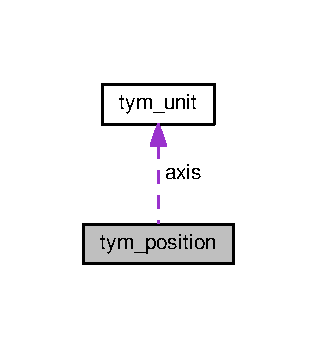
\includegraphics[width=152pt]{structtym__position__coll__graph}
\end{center}
\end{figure}
\subsection*{Data Fields}
\begin{DoxyCompactItemize}
\item 
enum \hyperlink{libttymultiplex_8h_a23b539c9dc1c137633f8783517fc2653}{tym\+\_\+position\+\_\+type} \hyperlink{structtym__position_a71682a3bc5e8e9e67f3cfadf0768d73d}{type}
\item 
struct \hyperlink{structtym__unit}{tym\+\_\+unit} \hyperlink{structtym__position_a1973e10af9a7a40d13da23ea6ec75b71}{axis} \mbox{[}\hyperlink{libttymultiplex_8h_a6b9111693b9da18b1f567760f5bc17beab5ce57254240d63c232aba1d7552322f}{T\+Y\+M\+\_\+\+A\+X\+I\+S\+\_\+\+C\+O\+U\+NT}\mbox{]}
\end{DoxyCompactItemize}


\subsection{Detailed Description}


Definition at line 124 of file libttymultiplex.\+h.



\subsection{Field Documentation}
\mbox{\Hypertarget{structtym__position_a1973e10af9a7a40d13da23ea6ec75b71}\label{structtym__position_a1973e10af9a7a40d13da23ea6ec75b71}} 
\index{tym\+\_\+position@{tym\+\_\+position}!axis@{axis}}
\index{axis@{axis}!tym\+\_\+position@{tym\+\_\+position}}
\subsubsection{\texorpdfstring{axis}{axis}}
{\footnotesize\ttfamily struct \hyperlink{structtym__unit}{tym\+\_\+unit} tym\+\_\+position\+::axis\mbox{[}\hyperlink{libttymultiplex_8h_a6b9111693b9da18b1f567760f5bc17beab5ce57254240d63c232aba1d7552322f}{T\+Y\+M\+\_\+\+A\+X\+I\+S\+\_\+\+C\+O\+U\+NT}\mbox{]}}



Definition at line 126 of file libttymultiplex.\+h.

\mbox{\Hypertarget{structtym__position_a71682a3bc5e8e9e67f3cfadf0768d73d}\label{structtym__position_a71682a3bc5e8e9e67f3cfadf0768d73d}} 
\index{tym\+\_\+position@{tym\+\_\+position}!type@{type}}
\index{type@{type}!tym\+\_\+position@{tym\+\_\+position}}
\subsubsection{\texorpdfstring{type}{type}}
{\footnotesize\ttfamily enum \hyperlink{libttymultiplex_8h_a23b539c9dc1c137633f8783517fc2653}{tym\+\_\+position\+\_\+type} tym\+\_\+position\+::type}



Definition at line 125 of file libttymultiplex.\+h.



The documentation for this struct was generated from the following file\+:\begin{DoxyCompactItemize}
\item 
include/\hyperlink{libttymultiplex_8h}{libttymultiplex.\+h}\end{DoxyCompactItemize}

\hypertarget{structtym__special__key__name}{}\section{tym\+\_\+special\+\_\+key\+\_\+name Struct Reference}
\label{structtym__special__key__name}\index{tym\+\_\+special\+\_\+key\+\_\+name@{tym\+\_\+special\+\_\+key\+\_\+name}}


{\ttfamily \#include $<$libttymultiplex.\+h$>$}

\subsection*{Data Fields}
\begin{DoxyCompactItemize}
\item 
enum \hyperlink{libttymultiplex_8h_abc86b175aee7ad5c631cdc10ff2025ac}{tym\+\_\+special\+\_\+key} \hyperlink{structtym__special__key__name_aebd783edb2f7d1252e28e7f1456d0757}{key}
\item 
const char $\ast$ \hyperlink{structtym__special__key__name_a9a82b9fd28fae482c836f959ca5a848b}{name}
\item 
size\+\_\+t \hyperlink{structtym__special__key__name_a6d6587d1d107252a68c6d9ab753d3ea6}{name\+\_\+length}
\end{DoxyCompactItemize}


\subsection{Detailed Description}


Definition at line 47 of file libttymultiplex.\+h.



\subsection{Field Documentation}
\mbox{\Hypertarget{structtym__special__key__name_aebd783edb2f7d1252e28e7f1456d0757}\label{structtym__special__key__name_aebd783edb2f7d1252e28e7f1456d0757}} 
\index{tym\+\_\+special\+\_\+key\+\_\+name@{tym\+\_\+special\+\_\+key\+\_\+name}!key@{key}}
\index{key@{key}!tym\+\_\+special\+\_\+key\+\_\+name@{tym\+\_\+special\+\_\+key\+\_\+name}}
\subsubsection{\texorpdfstring{key}{key}}
{\footnotesize\ttfamily enum \hyperlink{libttymultiplex_8h_abc86b175aee7ad5c631cdc10ff2025ac}{tym\+\_\+special\+\_\+key} tym\+\_\+special\+\_\+key\+\_\+name\+::key}



Definition at line 48 of file libttymultiplex.\+h.

\mbox{\Hypertarget{structtym__special__key__name_a9a82b9fd28fae482c836f959ca5a848b}\label{structtym__special__key__name_a9a82b9fd28fae482c836f959ca5a848b}} 
\index{tym\+\_\+special\+\_\+key\+\_\+name@{tym\+\_\+special\+\_\+key\+\_\+name}!name@{name}}
\index{name@{name}!tym\+\_\+special\+\_\+key\+\_\+name@{tym\+\_\+special\+\_\+key\+\_\+name}}
\subsubsection{\texorpdfstring{name}{name}}
{\footnotesize\ttfamily const char$\ast$ tym\+\_\+special\+\_\+key\+\_\+name\+::name}



Definition at line 49 of file libttymultiplex.\+h.

\mbox{\Hypertarget{structtym__special__key__name_a6d6587d1d107252a68c6d9ab753d3ea6}\label{structtym__special__key__name_a6d6587d1d107252a68c6d9ab753d3ea6}} 
\index{tym\+\_\+special\+\_\+key\+\_\+name@{tym\+\_\+special\+\_\+key\+\_\+name}!name\+\_\+length@{name\+\_\+length}}
\index{name\+\_\+length@{name\+\_\+length}!tym\+\_\+special\+\_\+key\+\_\+name@{tym\+\_\+special\+\_\+key\+\_\+name}}
\subsubsection{\texorpdfstring{name\+\_\+length}{name\_length}}
{\footnotesize\ttfamily size\+\_\+t tym\+\_\+special\+\_\+key\+\_\+name\+::name\+\_\+length}



Definition at line 50 of file libttymultiplex.\+h.



The documentation for this struct was generated from the following file\+:\begin{DoxyCompactItemize}
\item 
include/\hyperlink{libttymultiplex_8h}{libttymultiplex.\+h}\end{DoxyCompactItemize}

\hypertarget{structtym__super__position}{}\section{tym\+\_\+super\+\_\+position Struct Reference}
\label{structtym__super__position}\index{tym\+\_\+super\+\_\+position@{tym\+\_\+super\+\_\+position}}


{\ttfamily \#include $<$libttymultiplex.\+h$>$}



Collaboration diagram for tym\+\_\+super\+\_\+position\+:
\nopagebreak
\begin{figure}[H]
\begin{center}
\leavevmode
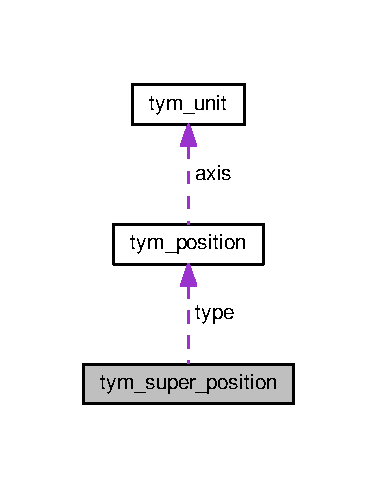
\includegraphics[width=181pt]{structtym__super__position__coll__graph}
\end{center}
\end{figure}
\subsection*{Data Fields}
\begin{DoxyCompactItemize}
\item 
struct \hyperlink{structtym__position}{tym\+\_\+position} \hyperlink{structtym__super__position_af5baedeebbc4d01a742503cf0536617c}{type} \mbox{[}\hyperlink{libttymultiplex_8h_a23b539c9dc1c137633f8783517fc2653a483bfa59d0a2b43731d992c418a42db7}{T\+Y\+M\+\_\+\+P\+\_\+\+C\+O\+U\+NT}\mbox{]}
\end{DoxyCompactItemize}


\subsection{Detailed Description}


Definition at line 137 of file libttymultiplex.\+h.



\subsection{Field Documentation}
\mbox{\Hypertarget{structtym__super__position_af5baedeebbc4d01a742503cf0536617c}\label{structtym__super__position_af5baedeebbc4d01a742503cf0536617c}} 
\index{tym\+\_\+super\+\_\+position@{tym\+\_\+super\+\_\+position}!type@{type}}
\index{type@{type}!tym\+\_\+super\+\_\+position@{tym\+\_\+super\+\_\+position}}
\subsubsection{\texorpdfstring{type}{type}}
{\footnotesize\ttfamily struct \hyperlink{structtym__position}{tym\+\_\+position} tym\+\_\+super\+\_\+position\+::type\mbox{[}\hyperlink{libttymultiplex_8h_a23b539c9dc1c137633f8783517fc2653a483bfa59d0a2b43731d992c418a42db7}{T\+Y\+M\+\_\+\+P\+\_\+\+C\+O\+U\+NT}\mbox{]}}



Definition at line 137 of file libttymultiplex.\+h.



The documentation for this struct was generated from the following file\+:\begin{DoxyCompactItemize}
\item 
include/\hyperlink{libttymultiplex_8h}{libttymultiplex.\+h}\end{DoxyCompactItemize}

\hypertarget{structtym__super__position__rectangle}{}\section{tym\+\_\+super\+\_\+position\+\_\+rectangle Struct Reference}
\label{structtym__super__position__rectangle}\index{tym\+\_\+super\+\_\+position\+\_\+rectangle@{tym\+\_\+super\+\_\+position\+\_\+rectangle}}


{\ttfamily \#include $<$libttymultiplex.\+h$>$}



Collaboration diagram for tym\+\_\+super\+\_\+position\+\_\+rectangle\+:
\nopagebreak
\begin{figure}[H]
\begin{center}
\leavevmode
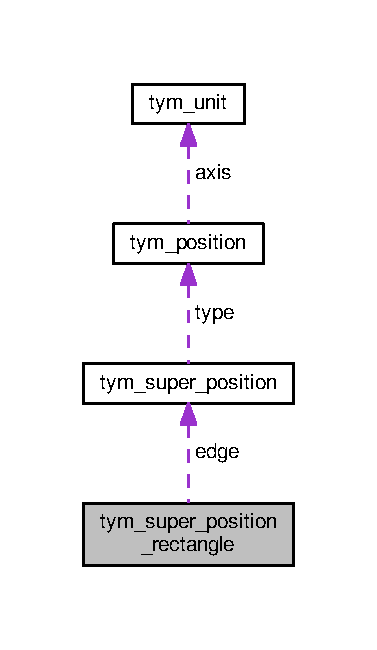
\includegraphics[width=181pt]{structtym__super__position__rectangle__coll__graph}
\end{center}
\end{figure}
\subsection*{Data Fields}
\begin{DoxyCompactItemize}
\item 
struct \hyperlink{structtym__super__position}{tym\+\_\+super\+\_\+position} \hyperlink{structtym__super__position__rectangle_aab3865c2a42bee957a40c0e8603d5a31}{edge} \mbox{[}\hyperlink{libttymultiplex_8h_ad8856480bf629c72938051528100b834ac0bfa9550b58bc257ca09715d719de7f}{T\+Y\+M\+\_\+\+E\+D\+G\+E\+\_\+\+C\+O\+U\+NT}\mbox{]}
\end{DoxyCompactItemize}


\subsection{Detailed Description}


Definition at line 137 of file libttymultiplex.\+h.



\subsection{Field Documentation}
\mbox{\Hypertarget{structtym__super__position__rectangle_aab3865c2a42bee957a40c0e8603d5a31}\label{structtym__super__position__rectangle_aab3865c2a42bee957a40c0e8603d5a31}} 
\index{tym\+\_\+super\+\_\+position\+\_\+rectangle@{tym\+\_\+super\+\_\+position\+\_\+rectangle}!edge@{edge}}
\index{edge@{edge}!tym\+\_\+super\+\_\+position\+\_\+rectangle@{tym\+\_\+super\+\_\+position\+\_\+rectangle}}
\subsubsection{\texorpdfstring{edge}{edge}}
{\footnotesize\ttfamily struct \hyperlink{structtym__super__position}{tym\+\_\+super\+\_\+position} tym\+\_\+super\+\_\+position\+\_\+rectangle\+::edge\mbox{[}\hyperlink{libttymultiplex_8h_ad8856480bf629c72938051528100b834ac0bfa9550b58bc257ca09715d719de7f}{T\+Y\+M\+\_\+\+E\+D\+G\+E\+\_\+\+C\+O\+U\+NT}\mbox{]}}



Definition at line 137 of file libttymultiplex.\+h.



The documentation for this struct was generated from the following file\+:\begin{DoxyCompactItemize}
\item 
include/\hyperlink{libttymultiplex_8h}{libttymultiplex.\+h}\end{DoxyCompactItemize}

\hypertarget{structtym__unit}{}\section{tym\+\_\+unit Struct Reference}
\label{structtym__unit}\index{tym\+\_\+unit@{tym\+\_\+unit}}


{\ttfamily \#include $<$libttymultiplex.\+h$>$}

\subsection*{Data Fields}
\begin{DoxyCompactItemize}
\item 
enum \hyperlink{libttymultiplex_8h_a11fda113de846a40d8d1851f94bc4415}{tym\+\_\+unit\+\_\+type} \hyperlink{structtym__unit_aa9af5f13506cbb15b261f7086cb16172}{type}
\item 
\begin{tabbing}
xx\=xx\=xx\=xx\=xx\=xx\=xx\=xx\=xx\=\kill
union \{\\
\>long \hyperlink{structtym__unit_ae3cab379eab2bf726b892c5ad9528368}{integer}\\
\>double \hyperlink{structtym__unit_a1335c8f102b171eae5743a25eaabb5ae}{real}\\
\} \hyperlink{structtym__unit_ab7efee5776cd58e5d8b6806e39a49c49}{value}\\

\end{tabbing}\end{DoxyCompactItemize}


\subsection{Detailed Description}


Definition at line 114 of file libttymultiplex.\+h.



\subsection{Field Documentation}
\mbox{\Hypertarget{structtym__unit_ae3cab379eab2bf726b892c5ad9528368}\label{structtym__unit_ae3cab379eab2bf726b892c5ad9528368}} 
\index{tym\+\_\+unit@{tym\+\_\+unit}!integer@{integer}}
\index{integer@{integer}!tym\+\_\+unit@{tym\+\_\+unit}}
\subsubsection{\texorpdfstring{integer}{integer}}
{\footnotesize\ttfamily long tym\+\_\+unit\+::integer}



Definition at line 119 of file libttymultiplex.\+h.

\mbox{\Hypertarget{structtym__unit_a1335c8f102b171eae5743a25eaabb5ae}\label{structtym__unit_a1335c8f102b171eae5743a25eaabb5ae}} 
\index{tym\+\_\+unit@{tym\+\_\+unit}!real@{real}}
\index{real@{real}!tym\+\_\+unit@{tym\+\_\+unit}}
\subsubsection{\texorpdfstring{real}{real}}
{\footnotesize\ttfamily double tym\+\_\+unit\+::real}



Definition at line 119 of file libttymultiplex.\+h.

\mbox{\Hypertarget{structtym__unit_aa9af5f13506cbb15b261f7086cb16172}\label{structtym__unit_aa9af5f13506cbb15b261f7086cb16172}} 
\index{tym\+\_\+unit@{tym\+\_\+unit}!type@{type}}
\index{type@{type}!tym\+\_\+unit@{tym\+\_\+unit}}
\subsubsection{\texorpdfstring{type}{type}}
{\footnotesize\ttfamily enum \hyperlink{libttymultiplex_8h_a11fda113de846a40d8d1851f94bc4415}{tym\+\_\+unit\+\_\+type} tym\+\_\+unit\+::type}



Definition at line 115 of file libttymultiplex.\+h.

\mbox{\Hypertarget{structtym__unit_ab7efee5776cd58e5d8b6806e39a49c49}\label{structtym__unit_ab7efee5776cd58e5d8b6806e39a49c49}} 
\index{tym\+\_\+unit@{tym\+\_\+unit}!value@{value}}
\index{value@{value}!tym\+\_\+unit@{tym\+\_\+unit}}
\subsubsection{\texorpdfstring{value}{value}}
{\footnotesize\ttfamily union \{ ... \}   tym\+\_\+unit\+::value}



The documentation for this struct was generated from the following file\+:\begin{DoxyCompactItemize}
\item 
include/\hyperlink{libttymultiplex_8h}{libttymultiplex.\+h}\end{DoxyCompactItemize}

\chapter{File Documentation}
\hypertarget{backend_8h}{}\section{include/internal/backend.h File Reference}
\label{backend_8h}\index{include/internal/backend.\+h@{include/internal/backend.\+h}}
{\ttfamily \#include $<$internal/utils.\+h$>$}\newline
{\ttfamily \#include $<$stdbool.\+h$>$}\newline
\subsection*{Data Structures}
\begin{DoxyCompactItemize}
\item 
struct \hyperlink{structtym__i__backend}{tym\+\_\+i\+\_\+backend}
\item 
struct \hyperlink{structtym__i__backend__entry}{tym\+\_\+i\+\_\+backend\+\_\+entry}
\end{DoxyCompactItemize}
\subsection*{Macros}
\begin{DoxyCompactItemize}
\item 
\#define \hyperlink{backend_8h_a36b5b58973bd499e27ef08efc073e7d8}{T\+Y\+M\+\_\+\+I\+\_\+\+B\+A\+C\+K\+E\+N\+D\+\_\+\+C\+A\+L\+L\+B\+A\+C\+KS}
\item 
\#define \hyperlink{backend_8h_a8704d4d8b7007b1dccbc67f47bbd19e4}{R}(R\+ET,  ID,  P\+A\+R\+A\+MS)~typedef R\+ET ($\ast$tym\+\_\+i\+\_\+ \#\# ID \#\# \+\_\+proc) P\+A\+R\+A\+MS;
\item 
\#define \hyperlink{backend_8h_acd1ff3ab6d4e5703f073e393248be973}{O}(R\+ET,  ID,  P\+A\+R\+A\+MS)~\hyperlink{backend_8h_a8704d4d8b7007b1dccbc67f47bbd19e4}{R}(R\+ET, ID, P\+A\+R\+A\+MS) R\+ET tym\+\_\+i\+\_\+ \#\# ID \#\# \+\_\+default\+\_\+proc P\+A\+R\+A\+MS;
\item 
\#define \hyperlink{backend_8h_a8704d4d8b7007b1dccbc67f47bbd19e4}{R}(R\+ET,  ID,  P\+A\+R\+A\+MS)~tym\+\_\+i\+\_\+ \#\# ID \#\# \+\_\+proc ID;
\item 
\#define \hyperlink{backend_8h_acd1ff3ab6d4e5703f073e393248be973}{O}(R\+ET,  ID,  P\+A\+R\+A\+MS)~\hyperlink{backend_8h_a8704d4d8b7007b1dccbc67f47bbd19e4}{R}(R\+ET, ID, P\+A\+R\+A\+MS)
\item 
\#define \hyperlink{backend_8h_aa9d0e93e983f5419b2c70dfd322d8f15}{T\+Y\+M\+\_\+\+I\+\_\+\+B\+A\+C\+K\+E\+N\+D\+\_\+\+R\+E\+G\+I\+S\+T\+ER}(P,  N,  X)
\end{DoxyCompactItemize}
\subsection*{Typedefs}
\begin{DoxyCompactItemize}
\item 
typedef int($\ast$ \hyperlink{backend_8h_a1d8c83e098af07295e7c8c6aaff509f8}{tym\+\_\+i\+\_\+init\+\_\+proc}) (void)
\item 
typedef int($\ast$ \hyperlink{backend_8h_a71c0f80d2ad6f4c617855bed5f727832}{tym\+\_\+i\+\_\+cleanup\+\_\+proc}) (void)
\item 
typedef int($\ast$ \hyperlink{backend_8h_a969a37c5dad74fed827c63879a3ea594}{tym\+\_\+i\+\_\+resize\+\_\+proc}) (void)
\item 
typedef int($\ast$ \hyperlink{backend_8h_ab44c405291766aa8377ccabbf142c682}{tym\+\_\+i\+\_\+pane\+\_\+create\+\_\+proc}) (struct \hyperlink{structtym__i__pane__internal}{tym\+\_\+i\+\_\+pane\+\_\+internal} $\ast$pane)
\item 
typedef void($\ast$ \hyperlink{backend_8h_a7c52fa9848f5daacdca285c8e25c6daf}{tym\+\_\+i\+\_\+pane\+\_\+destroy\+\_\+proc}) (struct \hyperlink{structtym__i__pane__internal}{tym\+\_\+i\+\_\+pane\+\_\+internal} $\ast$pane)
\item 
typedef int($\ast$ \hyperlink{backend_8h_ae66adc784ab9e9adcb7f43713798b754}{tym\+\_\+i\+\_\+pane\+\_\+resize\+\_\+proc}) (struct \hyperlink{structtym__i__pane__internal}{tym\+\_\+i\+\_\+pane\+\_\+internal} $\ast$pane)
\item 
typedef int($\ast$ \hyperlink{backend_8h_a8f701dd0984f9c7aa9f76fcd2df15a27}{tym\+\_\+i\+\_\+pane\+\_\+scroll\+\_\+region\+\_\+proc}) (struct \hyperlink{structtym__i__pane__internal}{tym\+\_\+i\+\_\+pane\+\_\+internal} $\ast$pane, int n, unsigned top, unsigned bottom)
\item 
typedef int($\ast$ \hyperlink{backend_8h_af5c21e9bc7ce1861a821cf0b8f3baa24}{tym\+\_\+i\+\_\+pane\+\_\+set\+\_\+cursor\+\_\+position\+\_\+proc}) (struct \hyperlink{structtym__i__pane__internal}{tym\+\_\+i\+\_\+pane\+\_\+internal} $\ast$pane, struct \hyperlink{structtym__i__cell__position}{tym\+\_\+i\+\_\+cell\+\_\+position} position)
\item 
typedef int($\ast$ \hyperlink{backend_8h_a4a3d0bb3b2fb6baa1f86e39770756a18}{tym\+\_\+i\+\_\+pane\+\_\+set\+\_\+character\+\_\+proc}) (struct \hyperlink{structtym__i__pane__internal}{tym\+\_\+i\+\_\+pane\+\_\+internal} $\ast$pane, struct \hyperlink{structtym__i__cell__position}{tym\+\_\+i\+\_\+cell\+\_\+position} position, struct \hyperlink{structtym__i__character__format}{tym\+\_\+i\+\_\+character\+\_\+format} format, size\+\_\+t length, const char utf8\mbox{[}length+1\mbox{]}, bool insert)
\item 
typedef int($\ast$ \hyperlink{backend_8h_a0926d88cba57a1e598f92df346d9d6a3}{tym\+\_\+i\+\_\+pane\+\_\+delete\+\_\+characters\+\_\+proc}) (struct \hyperlink{structtym__i__pane__internal}{tym\+\_\+i\+\_\+pane\+\_\+internal} $\ast$pane, struct \hyperlink{structtym__i__cell__position}{tym\+\_\+i\+\_\+cell\+\_\+position} position, unsigned n)
\item 
typedef int($\ast$ \hyperlink{backend_8h_a99b50ea4d7c5349b4df1e879b2140a97}{tym\+\_\+i\+\_\+pane\+\_\+refresh\+\_\+proc}) (struct \hyperlink{structtym__i__pane__internal}{tym\+\_\+i\+\_\+pane\+\_\+internal} $\ast$pane)
\item 
typedef int($\ast$ \hyperlink{backend_8h_a9488390b6c0e8e6ee6df0f65c0600033}{tym\+\_\+i\+\_\+pane\+\_\+set\+\_\+cursor\+\_\+mode\+\_\+proc}) (struct \hyperlink{structtym__i__pane__internal}{tym\+\_\+i\+\_\+pane\+\_\+internal} $\ast$pane, enum \hyperlink{backend_8h_abbe8b51b7d8c058f92aec216a1e3470c}{tym\+\_\+i\+\_\+cursor\+\_\+mode} cursor\+\_\+mode)
\item 
typedef int($\ast$ \hyperlink{backend_8h_ab44bedb286c42c2994bf88375e64176f}{tym\+\_\+i\+\_\+pane\+\_\+scroll\+\_\+proc}) (struct \hyperlink{structtym__i__pane__internal}{tym\+\_\+i\+\_\+pane\+\_\+internal} $\ast$pane, int n)
\item 
typedef int($\ast$ \hyperlink{backend_8h_a61a3d2bde17cca99666001e082332bc4}{tym\+\_\+i\+\_\+pane\+\_\+erase\+\_\+area\+\_\+proc}) (struct \hyperlink{structtym__i__pane__internal}{tym\+\_\+i\+\_\+pane\+\_\+internal} $\ast$pane, struct \hyperlink{structtym__i__cell__position}{tym\+\_\+i\+\_\+cell\+\_\+position} start, struct \hyperlink{structtym__i__cell__position}{tym\+\_\+i\+\_\+cell\+\_\+position} end, bool block, struct \hyperlink{structtym__i__character__format}{tym\+\_\+i\+\_\+character\+\_\+format} format)
\item 
typedef int($\ast$ \hyperlink{backend_8h_a069b99db5129d301726cec915fea32a8}{tym\+\_\+i\+\_\+pane\+\_\+change\+\_\+screen\+\_\+proc}) (struct \hyperlink{structtym__i__pane__internal}{tym\+\_\+i\+\_\+pane\+\_\+internal} $\ast$pane)
\item 
typedef int($\ast$ \hyperlink{backend_8h_aaaee2104d442c8976abfd9228375c878}{tym\+\_\+i\+\_\+pane\+\_\+set\+\_\+area\+\_\+to\+\_\+character\+\_\+proc}) (struct \hyperlink{structtym__i__pane__internal}{tym\+\_\+i\+\_\+pane\+\_\+internal} $\ast$pane, struct \hyperlink{structtym__i__cell__position}{tym\+\_\+i\+\_\+cell\+\_\+position} start, struct \hyperlink{structtym__i__cell__position}{tym\+\_\+i\+\_\+cell\+\_\+position} end, bool block, struct \hyperlink{structtym__i__character__format}{tym\+\_\+i\+\_\+character\+\_\+format} format, size\+\_\+t length, const char utf8\mbox{[}length+1\mbox{]})
\end{DoxyCompactItemize}
\subsection*{Enumerations}
\begin{DoxyCompactItemize}
\item 
enum \hyperlink{backend_8h_abbe8b51b7d8c058f92aec216a1e3470c}{tym\+\_\+i\+\_\+cursor\+\_\+mode} \{ \newline
\hyperlink{backend_8h_abbe8b51b7d8c058f92aec216a1e3470ca0b3a0191b02a94b58a9698d1b7ad0023}{T\+Y\+M\+\_\+\+I\+\_\+\+C\+U\+R\+S\+O\+R\+\_\+\+B\+L\+O\+CK}, 
\newline
\hyperlink{backend_8h_abbe8b51b7d8c058f92aec216a1e3470ca83752a04a8080057c727fe0965ef92a0}{T\+Y\+M\+\_\+\+I\+\_\+\+C\+U\+R\+S\+O\+R\+\_\+\+U\+N\+D\+E\+R\+L\+I\+NE}, 
\newline
\hyperlink{backend_8h_abbe8b51b7d8c058f92aec216a1e3470cabacc8b6592ec667df788dc572c678209}{T\+Y\+M\+\_\+\+I\+\_\+\+C\+U\+R\+S\+O\+R\+\_\+\+N\+O\+NE}
 \}
\end{DoxyCompactItemize}
\subsection*{Functions}
\begin{DoxyCompactItemize}
\item 
int \hyperlink{backend_8h_a34e3a9047936ef5683db1bf03ad80157}{tym\+\_\+i\+\_\+pane\+\_\+refresh\+\_\+default\+\_\+proc} (struct \hyperlink{structtym__i__pane__internal}{tym\+\_\+i\+\_\+pane\+\_\+internal} $\ast$pane)
\item 
int \hyperlink{backend_8h_a8f80296bf84bca064c055fdf0e2a6e6a}{tym\+\_\+i\+\_\+pane\+\_\+set\+\_\+cursor\+\_\+mode\+\_\+default\+\_\+proc} (struct \hyperlink{structtym__i__pane__internal}{tym\+\_\+i\+\_\+pane\+\_\+internal} $\ast$pane, enum \hyperlink{backend_8h_abbe8b51b7d8c058f92aec216a1e3470c}{tym\+\_\+i\+\_\+cursor\+\_\+mode} cursor\+\_\+mode)
\item 
int \hyperlink{backend_8h_a26b2409a9fdd7a7e3ccf51d29411398d}{tym\+\_\+i\+\_\+pane\+\_\+scroll\+\_\+default\+\_\+proc} (struct \hyperlink{structtym__i__pane__internal}{tym\+\_\+i\+\_\+pane\+\_\+internal} $\ast$pane, int n)
\item 
int \hyperlink{backend_8h_a3f761d347e4888f8e839135e1fce98d7}{tym\+\_\+i\+\_\+pane\+\_\+erase\+\_\+area\+\_\+default\+\_\+proc} (struct \hyperlink{structtym__i__pane__internal}{tym\+\_\+i\+\_\+pane\+\_\+internal} $\ast$pane, struct \hyperlink{structtym__i__cell__position}{tym\+\_\+i\+\_\+cell\+\_\+position} start, struct \hyperlink{structtym__i__cell__position}{tym\+\_\+i\+\_\+cell\+\_\+position} end, bool block, struct \hyperlink{structtym__i__character__format}{tym\+\_\+i\+\_\+character\+\_\+format} format)
\item 
int \hyperlink{backend_8h_a9298fc19b3f6fe589590a850e2f5cf7f}{tym\+\_\+i\+\_\+pane\+\_\+change\+\_\+screen\+\_\+default\+\_\+proc} (struct \hyperlink{structtym__i__pane__internal}{tym\+\_\+i\+\_\+pane\+\_\+internal} $\ast$pane)
\item 
int \hyperlink{backend_8h_ae7ca7572e887bdc29177974c2862fce4}{tym\+\_\+i\+\_\+pane\+\_\+set\+\_\+area\+\_\+to\+\_\+character\+\_\+default\+\_\+proc} (struct \hyperlink{structtym__i__pane__internal}{tym\+\_\+i\+\_\+pane\+\_\+internal} $\ast$pane, struct \hyperlink{structtym__i__cell__position}{tym\+\_\+i\+\_\+cell\+\_\+position} start, struct \hyperlink{structtym__i__cell__position}{tym\+\_\+i\+\_\+cell\+\_\+position} end, bool block, struct \hyperlink{structtym__i__character__format}{tym\+\_\+i\+\_\+character\+\_\+format} format, size\+\_\+t length, const char utf8\mbox{[}length+1\mbox{]})
\item 
void \hyperlink{backend_8h_a41a24f368e837c5ef95ccf2ec0a89031}{tym\+\_\+i\+\_\+backend\+\_\+register} (struct \hyperlink{structtym__i__backend__entry}{tym\+\_\+i\+\_\+backend\+\_\+entry} $\ast$entry)
\item 
int \hyperlink{backend_8h_a015a67277bad329470d666c7af87c255}{tym\+\_\+i\+\_\+backend\+\_\+init} (const char $\ast$backend)
\end{DoxyCompactItemize}
\subsection*{Variables}
\begin{DoxyCompactItemize}
\item 
const struct \hyperlink{structtym__i__backend}{tym\+\_\+i\+\_\+backend} $\ast$ \hyperlink{backend_8h_afafbc6e2f17c4286715bc5f2aae23616}{tym\+\_\+i\+\_\+backend}
\end{DoxyCompactItemize}


\subsection{Macro Definition Documentation}
\mbox{\Hypertarget{backend_8h_acd1ff3ab6d4e5703f073e393248be973}\label{backend_8h_acd1ff3ab6d4e5703f073e393248be973}} 
\index{backend.\+h@{backend.\+h}!O@{O}}
\index{O@{O}!backend.\+h@{backend.\+h}}
\subsubsection{\texorpdfstring{O}{O}\hspace{0.1cm}{\footnotesize\ttfamily [1/2]}}
{\footnotesize\ttfamily \#define O(\begin{DoxyParamCaption}\item[{}]{R\+ET,  }\item[{}]{ID,  }\item[{}]{P\+A\+R\+A\+MS }\end{DoxyParamCaption})~\hyperlink{backend_8h_a8704d4d8b7007b1dccbc67f47bbd19e4}{R}(R\+ET, ID, P\+A\+R\+A\+MS) R\+ET tym\+\_\+i\+\_\+ \#\# ID \#\# \+\_\+default\+\_\+proc P\+A\+R\+A\+MS;}



Definition at line 67 of file backend.\+h.

\mbox{\Hypertarget{backend_8h_acd1ff3ab6d4e5703f073e393248be973}\label{backend_8h_acd1ff3ab6d4e5703f073e393248be973}} 
\index{backend.\+h@{backend.\+h}!O@{O}}
\index{O@{O}!backend.\+h@{backend.\+h}}
\subsubsection{\texorpdfstring{O}{O}\hspace{0.1cm}{\footnotesize\ttfamily [2/2]}}
{\footnotesize\ttfamily \#define O(\begin{DoxyParamCaption}\item[{}]{R\+ET,  }\item[{}]{ID,  }\item[{}]{P\+A\+R\+A\+MS }\end{DoxyParamCaption})~\hyperlink{backend_8h_a8704d4d8b7007b1dccbc67f47bbd19e4}{R}(R\+ET, ID, P\+A\+R\+A\+MS)}



Definition at line 67 of file backend.\+h.

\mbox{\Hypertarget{backend_8h_a8704d4d8b7007b1dccbc67f47bbd19e4}\label{backend_8h_a8704d4d8b7007b1dccbc67f47bbd19e4}} 
\index{backend.\+h@{backend.\+h}!R@{R}}
\index{R@{R}!backend.\+h@{backend.\+h}}
\subsubsection{\texorpdfstring{R}{R}\hspace{0.1cm}{\footnotesize\ttfamily [1/2]}}
{\footnotesize\ttfamily \#define R(\begin{DoxyParamCaption}\item[{}]{R\+ET,  }\item[{}]{ID,  }\item[{}]{P\+A\+R\+A\+MS }\end{DoxyParamCaption})~typedef R\+ET ($\ast$tym\+\_\+i\+\_\+ \#\# ID \#\# \+\_\+proc) P\+A\+R\+A\+MS;}



Definition at line 66 of file backend.\+h.

\mbox{\Hypertarget{backend_8h_a8704d4d8b7007b1dccbc67f47bbd19e4}\label{backend_8h_a8704d4d8b7007b1dccbc67f47bbd19e4}} 
\index{backend.\+h@{backend.\+h}!R@{R}}
\index{R@{R}!backend.\+h@{backend.\+h}}
\subsubsection{\texorpdfstring{R}{R}\hspace{0.1cm}{\footnotesize\ttfamily [2/2]}}
{\footnotesize\ttfamily \#define R(\begin{DoxyParamCaption}\item[{}]{R\+ET,  }\item[{}]{ID,  }\item[{}]{P\+A\+R\+A\+MS }\end{DoxyParamCaption})~tym\+\_\+i\+\_\+ \#\# ID \#\# \+\_\+proc ID;}



Definition at line 66 of file backend.\+h.

\mbox{\Hypertarget{backend_8h_a36b5b58973bd499e27ef08efc073e7d8}\label{backend_8h_a36b5b58973bd499e27ef08efc073e7d8}} 
\index{backend.\+h@{backend.\+h}!T\+Y\+M\+\_\+\+I\+\_\+\+B\+A\+C\+K\+E\+N\+D\+\_\+\+C\+A\+L\+L\+B\+A\+C\+KS@{T\+Y\+M\+\_\+\+I\+\_\+\+B\+A\+C\+K\+E\+N\+D\+\_\+\+C\+A\+L\+L\+B\+A\+C\+KS}}
\index{T\+Y\+M\+\_\+\+I\+\_\+\+B\+A\+C\+K\+E\+N\+D\+\_\+\+C\+A\+L\+L\+B\+A\+C\+KS@{T\+Y\+M\+\_\+\+I\+\_\+\+B\+A\+C\+K\+E\+N\+D\+\_\+\+C\+A\+L\+L\+B\+A\+C\+KS}!backend.\+h@{backend.\+h}}
\subsubsection{\texorpdfstring{T\+Y\+M\+\_\+\+I\+\_\+\+B\+A\+C\+K\+E\+N\+D\+\_\+\+C\+A\+L\+L\+B\+A\+C\+KS}{TYM\_I\_BACKEND\_CALLBACKS}}
{\footnotesize\ttfamily \#define T\+Y\+M\+\_\+\+I\+\_\+\+B\+A\+C\+K\+E\+N\+D\+\_\+\+C\+A\+L\+L\+B\+A\+C\+KS}



Definition at line 20 of file backend.\+h.

\mbox{\Hypertarget{backend_8h_aa9d0e93e983f5419b2c70dfd322d8f15}\label{backend_8h_aa9d0e93e983f5419b2c70dfd322d8f15}} 
\index{backend.\+h@{backend.\+h}!T\+Y\+M\+\_\+\+I\+\_\+\+B\+A\+C\+K\+E\+N\+D\+\_\+\+R\+E\+G\+I\+S\+T\+ER@{T\+Y\+M\+\_\+\+I\+\_\+\+B\+A\+C\+K\+E\+N\+D\+\_\+\+R\+E\+G\+I\+S\+T\+ER}}
\index{T\+Y\+M\+\_\+\+I\+\_\+\+B\+A\+C\+K\+E\+N\+D\+\_\+\+R\+E\+G\+I\+S\+T\+ER@{T\+Y\+M\+\_\+\+I\+\_\+\+B\+A\+C\+K\+E\+N\+D\+\_\+\+R\+E\+G\+I\+S\+T\+ER}!backend.\+h@{backend.\+h}}
\subsubsection{\texorpdfstring{T\+Y\+M\+\_\+\+I\+\_\+\+B\+A\+C\+K\+E\+N\+D\+\_\+\+R\+E\+G\+I\+S\+T\+ER}{TYM\_I\_BACKEND\_REGISTER}}
{\footnotesize\ttfamily \#define T\+Y\+M\+\_\+\+I\+\_\+\+B\+A\+C\+K\+E\+N\+D\+\_\+\+R\+E\+G\+I\+S\+T\+ER(\begin{DoxyParamCaption}\item[{}]{P,  }\item[{}]{N,  }\item[{}]{X }\end{DoxyParamCaption})}

{\bfseries Value\+:}
\begin{DoxyCode}
\textcolor{keyword}{static} \textcolor{keywordtype}{void} \hyperlink{utils_8h_a0d24a121c7f16b2b92d9b55b114c15fa}{TYM\_LUNIQUE}(register\_backend)(void) \_\_attribute\_\_((constructor(P),used)); \(\backslash\)
  static \textcolor{keywordtype}{void} \hyperlink{utils_8h_a0d24a121c7f16b2b92d9b55b114c15fa}{TYM\_LUNIQUE}(register\_backend)(void)\{ \(\backslash\)
    static \textcolor{keyword}{struct }\hyperlink{structtym__i__backend__entry}{tym\_i\_backend\_entry} entry = \{ \(\backslash\)
      .\hyperlink{structtym__i__backend__entry_abc39107ed565fd8c35370447417eedfc}{name} = N, \(\backslash\)
      .backend = \{ \hyperlink{utils_8h_a6a50bc6ecc9744410716ac50bd11287a}{TYM\_UNPACK} X \} \(\backslash\)
    \}; \(\backslash\)
    tym\_i\_backend\_register(&entry); \(\backslash\)
  \}
\end{DoxyCode}


Definition at line 84 of file backend.\+h.



\subsection{Typedef Documentation}
\mbox{\Hypertarget{backend_8h_a71c0f80d2ad6f4c617855bed5f727832}\label{backend_8h_a71c0f80d2ad6f4c617855bed5f727832}} 
\index{backend.\+h@{backend.\+h}!tym\+\_\+i\+\_\+cleanup\+\_\+proc@{tym\+\_\+i\+\_\+cleanup\+\_\+proc}}
\index{tym\+\_\+i\+\_\+cleanup\+\_\+proc@{tym\+\_\+i\+\_\+cleanup\+\_\+proc}!backend.\+h@{backend.\+h}}
\subsubsection{\texorpdfstring{tym\+\_\+i\+\_\+cleanup\+\_\+proc}{tym\_i\_cleanup\_proc}}
{\footnotesize\ttfamily typedef int($\ast$ tym\+\_\+i\+\_\+cleanup\+\_\+proc) (void)}



Definition at line 61 of file backend.\+h.

\mbox{\Hypertarget{backend_8h_a1d8c83e098af07295e7c8c6aaff509f8}\label{backend_8h_a1d8c83e098af07295e7c8c6aaff509f8}} 
\index{backend.\+h@{backend.\+h}!tym\+\_\+i\+\_\+init\+\_\+proc@{tym\+\_\+i\+\_\+init\+\_\+proc}}
\index{tym\+\_\+i\+\_\+init\+\_\+proc@{tym\+\_\+i\+\_\+init\+\_\+proc}!backend.\+h@{backend.\+h}}
\subsubsection{\texorpdfstring{tym\+\_\+i\+\_\+init\+\_\+proc}{tym\_i\_init\_proc}}
{\footnotesize\ttfamily typedef int($\ast$ tym\+\_\+i\+\_\+init\+\_\+proc) (void)}



Definition at line 61 of file backend.\+h.

\mbox{\Hypertarget{backend_8h_a069b99db5129d301726cec915fea32a8}\label{backend_8h_a069b99db5129d301726cec915fea32a8}} 
\index{backend.\+h@{backend.\+h}!tym\+\_\+i\+\_\+pane\+\_\+change\+\_\+screen\+\_\+proc@{tym\+\_\+i\+\_\+pane\+\_\+change\+\_\+screen\+\_\+proc}}
\index{tym\+\_\+i\+\_\+pane\+\_\+change\+\_\+screen\+\_\+proc@{tym\+\_\+i\+\_\+pane\+\_\+change\+\_\+screen\+\_\+proc}!backend.\+h@{backend.\+h}}
\subsubsection{\texorpdfstring{tym\+\_\+i\+\_\+pane\+\_\+change\+\_\+screen\+\_\+proc}{tym\_i\_pane\_change\_screen\_proc}}
{\footnotesize\ttfamily typedef int($\ast$ tym\+\_\+i\+\_\+pane\+\_\+change\+\_\+screen\+\_\+proc) (struct \hyperlink{structtym__i__pane__internal}{tym\+\_\+i\+\_\+pane\+\_\+internal} $\ast$pane)}



Definition at line 61 of file backend.\+h.

\mbox{\Hypertarget{backend_8h_ab44c405291766aa8377ccabbf142c682}\label{backend_8h_ab44c405291766aa8377ccabbf142c682}} 
\index{backend.\+h@{backend.\+h}!tym\+\_\+i\+\_\+pane\+\_\+create\+\_\+proc@{tym\+\_\+i\+\_\+pane\+\_\+create\+\_\+proc}}
\index{tym\+\_\+i\+\_\+pane\+\_\+create\+\_\+proc@{tym\+\_\+i\+\_\+pane\+\_\+create\+\_\+proc}!backend.\+h@{backend.\+h}}
\subsubsection{\texorpdfstring{tym\+\_\+i\+\_\+pane\+\_\+create\+\_\+proc}{tym\_i\_pane\_create\_proc}}
{\footnotesize\ttfamily typedef int($\ast$ tym\+\_\+i\+\_\+pane\+\_\+create\+\_\+proc) (struct \hyperlink{structtym__i__pane__internal}{tym\+\_\+i\+\_\+pane\+\_\+internal} $\ast$pane)}



Definition at line 61 of file backend.\+h.

\mbox{\Hypertarget{backend_8h_a0926d88cba57a1e598f92df346d9d6a3}\label{backend_8h_a0926d88cba57a1e598f92df346d9d6a3}} 
\index{backend.\+h@{backend.\+h}!tym\+\_\+i\+\_\+pane\+\_\+delete\+\_\+characters\+\_\+proc@{tym\+\_\+i\+\_\+pane\+\_\+delete\+\_\+characters\+\_\+proc}}
\index{tym\+\_\+i\+\_\+pane\+\_\+delete\+\_\+characters\+\_\+proc@{tym\+\_\+i\+\_\+pane\+\_\+delete\+\_\+characters\+\_\+proc}!backend.\+h@{backend.\+h}}
\subsubsection{\texorpdfstring{tym\+\_\+i\+\_\+pane\+\_\+delete\+\_\+characters\+\_\+proc}{tym\_i\_pane\_delete\_characters\_proc}}
{\footnotesize\ttfamily typedef int($\ast$ tym\+\_\+i\+\_\+pane\+\_\+delete\+\_\+characters\+\_\+proc) (struct \hyperlink{structtym__i__pane__internal}{tym\+\_\+i\+\_\+pane\+\_\+internal} $\ast$pane, struct \hyperlink{structtym__i__cell__position}{tym\+\_\+i\+\_\+cell\+\_\+position} position, unsigned n)}



Definition at line 61 of file backend.\+h.

\mbox{\Hypertarget{backend_8h_a7c52fa9848f5daacdca285c8e25c6daf}\label{backend_8h_a7c52fa9848f5daacdca285c8e25c6daf}} 
\index{backend.\+h@{backend.\+h}!tym\+\_\+i\+\_\+pane\+\_\+destroy\+\_\+proc@{tym\+\_\+i\+\_\+pane\+\_\+destroy\+\_\+proc}}
\index{tym\+\_\+i\+\_\+pane\+\_\+destroy\+\_\+proc@{tym\+\_\+i\+\_\+pane\+\_\+destroy\+\_\+proc}!backend.\+h@{backend.\+h}}
\subsubsection{\texorpdfstring{tym\+\_\+i\+\_\+pane\+\_\+destroy\+\_\+proc}{tym\_i\_pane\_destroy\_proc}}
{\footnotesize\ttfamily typedef void($\ast$ tym\+\_\+i\+\_\+pane\+\_\+destroy\+\_\+proc) (struct \hyperlink{structtym__i__pane__internal}{tym\+\_\+i\+\_\+pane\+\_\+internal} $\ast$pane)}



Definition at line 61 of file backend.\+h.

\mbox{\Hypertarget{backend_8h_a61a3d2bde17cca99666001e082332bc4}\label{backend_8h_a61a3d2bde17cca99666001e082332bc4}} 
\index{backend.\+h@{backend.\+h}!tym\+\_\+i\+\_\+pane\+\_\+erase\+\_\+area\+\_\+proc@{tym\+\_\+i\+\_\+pane\+\_\+erase\+\_\+area\+\_\+proc}}
\index{tym\+\_\+i\+\_\+pane\+\_\+erase\+\_\+area\+\_\+proc@{tym\+\_\+i\+\_\+pane\+\_\+erase\+\_\+area\+\_\+proc}!backend.\+h@{backend.\+h}}
\subsubsection{\texorpdfstring{tym\+\_\+i\+\_\+pane\+\_\+erase\+\_\+area\+\_\+proc}{tym\_i\_pane\_erase\_area\_proc}}
{\footnotesize\ttfamily typedef int($\ast$ tym\+\_\+i\+\_\+pane\+\_\+erase\+\_\+area\+\_\+proc) (struct \hyperlink{structtym__i__pane__internal}{tym\+\_\+i\+\_\+pane\+\_\+internal} $\ast$pane, struct \hyperlink{structtym__i__cell__position}{tym\+\_\+i\+\_\+cell\+\_\+position} start, struct \hyperlink{structtym__i__cell__position}{tym\+\_\+i\+\_\+cell\+\_\+position} end, bool block, struct \hyperlink{structtym__i__character__format}{tym\+\_\+i\+\_\+character\+\_\+format} format)}



Definition at line 61 of file backend.\+h.

\mbox{\Hypertarget{backend_8h_a99b50ea4d7c5349b4df1e879b2140a97}\label{backend_8h_a99b50ea4d7c5349b4df1e879b2140a97}} 
\index{backend.\+h@{backend.\+h}!tym\+\_\+i\+\_\+pane\+\_\+refresh\+\_\+proc@{tym\+\_\+i\+\_\+pane\+\_\+refresh\+\_\+proc}}
\index{tym\+\_\+i\+\_\+pane\+\_\+refresh\+\_\+proc@{tym\+\_\+i\+\_\+pane\+\_\+refresh\+\_\+proc}!backend.\+h@{backend.\+h}}
\subsubsection{\texorpdfstring{tym\+\_\+i\+\_\+pane\+\_\+refresh\+\_\+proc}{tym\_i\_pane\_refresh\_proc}}
{\footnotesize\ttfamily typedef int($\ast$ tym\+\_\+i\+\_\+pane\+\_\+refresh\+\_\+proc) (struct \hyperlink{structtym__i__pane__internal}{tym\+\_\+i\+\_\+pane\+\_\+internal} $\ast$pane)}



Definition at line 61 of file backend.\+h.

\mbox{\Hypertarget{backend_8h_ae66adc784ab9e9adcb7f43713798b754}\label{backend_8h_ae66adc784ab9e9adcb7f43713798b754}} 
\index{backend.\+h@{backend.\+h}!tym\+\_\+i\+\_\+pane\+\_\+resize\+\_\+proc@{tym\+\_\+i\+\_\+pane\+\_\+resize\+\_\+proc}}
\index{tym\+\_\+i\+\_\+pane\+\_\+resize\+\_\+proc@{tym\+\_\+i\+\_\+pane\+\_\+resize\+\_\+proc}!backend.\+h@{backend.\+h}}
\subsubsection{\texorpdfstring{tym\+\_\+i\+\_\+pane\+\_\+resize\+\_\+proc}{tym\_i\_pane\_resize\_proc}}
{\footnotesize\ttfamily typedef int($\ast$ tym\+\_\+i\+\_\+pane\+\_\+resize\+\_\+proc) (struct \hyperlink{structtym__i__pane__internal}{tym\+\_\+i\+\_\+pane\+\_\+internal} $\ast$pane)}



Definition at line 61 of file backend.\+h.

\mbox{\Hypertarget{backend_8h_ab44bedb286c42c2994bf88375e64176f}\label{backend_8h_ab44bedb286c42c2994bf88375e64176f}} 
\index{backend.\+h@{backend.\+h}!tym\+\_\+i\+\_\+pane\+\_\+scroll\+\_\+proc@{tym\+\_\+i\+\_\+pane\+\_\+scroll\+\_\+proc}}
\index{tym\+\_\+i\+\_\+pane\+\_\+scroll\+\_\+proc@{tym\+\_\+i\+\_\+pane\+\_\+scroll\+\_\+proc}!backend.\+h@{backend.\+h}}
\subsubsection{\texorpdfstring{tym\+\_\+i\+\_\+pane\+\_\+scroll\+\_\+proc}{tym\_i\_pane\_scroll\_proc}}
{\footnotesize\ttfamily typedef int($\ast$ tym\+\_\+i\+\_\+pane\+\_\+scroll\+\_\+proc) (struct \hyperlink{structtym__i__pane__internal}{tym\+\_\+i\+\_\+pane\+\_\+internal} $\ast$pane, int n)}



Definition at line 61 of file backend.\+h.

\mbox{\Hypertarget{backend_8h_a8f701dd0984f9c7aa9f76fcd2df15a27}\label{backend_8h_a8f701dd0984f9c7aa9f76fcd2df15a27}} 
\index{backend.\+h@{backend.\+h}!tym\+\_\+i\+\_\+pane\+\_\+scroll\+\_\+region\+\_\+proc@{tym\+\_\+i\+\_\+pane\+\_\+scroll\+\_\+region\+\_\+proc}}
\index{tym\+\_\+i\+\_\+pane\+\_\+scroll\+\_\+region\+\_\+proc@{tym\+\_\+i\+\_\+pane\+\_\+scroll\+\_\+region\+\_\+proc}!backend.\+h@{backend.\+h}}
\subsubsection{\texorpdfstring{tym\+\_\+i\+\_\+pane\+\_\+scroll\+\_\+region\+\_\+proc}{tym\_i\_pane\_scroll\_region\_proc}}
{\footnotesize\ttfamily typedef int($\ast$ tym\+\_\+i\+\_\+pane\+\_\+scroll\+\_\+region\+\_\+proc) (struct \hyperlink{structtym__i__pane__internal}{tym\+\_\+i\+\_\+pane\+\_\+internal} $\ast$pane, int n, unsigned top, unsigned bottom)}



Definition at line 61 of file backend.\+h.

\mbox{\Hypertarget{backend_8h_aaaee2104d442c8976abfd9228375c878}\label{backend_8h_aaaee2104d442c8976abfd9228375c878}} 
\index{backend.\+h@{backend.\+h}!tym\+\_\+i\+\_\+pane\+\_\+set\+\_\+area\+\_\+to\+\_\+character\+\_\+proc@{tym\+\_\+i\+\_\+pane\+\_\+set\+\_\+area\+\_\+to\+\_\+character\+\_\+proc}}
\index{tym\+\_\+i\+\_\+pane\+\_\+set\+\_\+area\+\_\+to\+\_\+character\+\_\+proc@{tym\+\_\+i\+\_\+pane\+\_\+set\+\_\+area\+\_\+to\+\_\+character\+\_\+proc}!backend.\+h@{backend.\+h}}
\subsubsection{\texorpdfstring{tym\+\_\+i\+\_\+pane\+\_\+set\+\_\+area\+\_\+to\+\_\+character\+\_\+proc}{tym\_i\_pane\_set\_area\_to\_character\_proc}}
{\footnotesize\ttfamily typedef int($\ast$ tym\+\_\+i\+\_\+pane\+\_\+set\+\_\+area\+\_\+to\+\_\+character\+\_\+proc) (struct \hyperlink{structtym__i__pane__internal}{tym\+\_\+i\+\_\+pane\+\_\+internal} $\ast$pane, struct \hyperlink{structtym__i__cell__position}{tym\+\_\+i\+\_\+cell\+\_\+position} start, struct \hyperlink{structtym__i__cell__position}{tym\+\_\+i\+\_\+cell\+\_\+position} end, bool block, struct \hyperlink{structtym__i__character__format}{tym\+\_\+i\+\_\+character\+\_\+format} format, size\+\_\+t length, const char utf8\mbox{[}length+1\mbox{]})}



Definition at line 61 of file backend.\+h.

\mbox{\Hypertarget{backend_8h_a4a3d0bb3b2fb6baa1f86e39770756a18}\label{backend_8h_a4a3d0bb3b2fb6baa1f86e39770756a18}} 
\index{backend.\+h@{backend.\+h}!tym\+\_\+i\+\_\+pane\+\_\+set\+\_\+character\+\_\+proc@{tym\+\_\+i\+\_\+pane\+\_\+set\+\_\+character\+\_\+proc}}
\index{tym\+\_\+i\+\_\+pane\+\_\+set\+\_\+character\+\_\+proc@{tym\+\_\+i\+\_\+pane\+\_\+set\+\_\+character\+\_\+proc}!backend.\+h@{backend.\+h}}
\subsubsection{\texorpdfstring{tym\+\_\+i\+\_\+pane\+\_\+set\+\_\+character\+\_\+proc}{tym\_i\_pane\_set\_character\_proc}}
{\footnotesize\ttfamily typedef int($\ast$ tym\+\_\+i\+\_\+pane\+\_\+set\+\_\+character\+\_\+proc) (struct \hyperlink{structtym__i__pane__internal}{tym\+\_\+i\+\_\+pane\+\_\+internal} $\ast$pane, struct \hyperlink{structtym__i__cell__position}{tym\+\_\+i\+\_\+cell\+\_\+position} position, struct \hyperlink{structtym__i__character__format}{tym\+\_\+i\+\_\+character\+\_\+format} format, size\+\_\+t length, const char utf8\mbox{[}length+1\mbox{]}, bool insert)}



Definition at line 61 of file backend.\+h.

\mbox{\Hypertarget{backend_8h_a9488390b6c0e8e6ee6df0f65c0600033}\label{backend_8h_a9488390b6c0e8e6ee6df0f65c0600033}} 
\index{backend.\+h@{backend.\+h}!tym\+\_\+i\+\_\+pane\+\_\+set\+\_\+cursor\+\_\+mode\+\_\+proc@{tym\+\_\+i\+\_\+pane\+\_\+set\+\_\+cursor\+\_\+mode\+\_\+proc}}
\index{tym\+\_\+i\+\_\+pane\+\_\+set\+\_\+cursor\+\_\+mode\+\_\+proc@{tym\+\_\+i\+\_\+pane\+\_\+set\+\_\+cursor\+\_\+mode\+\_\+proc}!backend.\+h@{backend.\+h}}
\subsubsection{\texorpdfstring{tym\+\_\+i\+\_\+pane\+\_\+set\+\_\+cursor\+\_\+mode\+\_\+proc}{tym\_i\_pane\_set\_cursor\_mode\_proc}}
{\footnotesize\ttfamily typedef int($\ast$ tym\+\_\+i\+\_\+pane\+\_\+set\+\_\+cursor\+\_\+mode\+\_\+proc) (struct \hyperlink{structtym__i__pane__internal}{tym\+\_\+i\+\_\+pane\+\_\+internal} $\ast$pane, enum \hyperlink{backend_8h_abbe8b51b7d8c058f92aec216a1e3470c}{tym\+\_\+i\+\_\+cursor\+\_\+mode} cursor\+\_\+mode)}



Definition at line 61 of file backend.\+h.

\mbox{\Hypertarget{backend_8h_af5c21e9bc7ce1861a821cf0b8f3baa24}\label{backend_8h_af5c21e9bc7ce1861a821cf0b8f3baa24}} 
\index{backend.\+h@{backend.\+h}!tym\+\_\+i\+\_\+pane\+\_\+set\+\_\+cursor\+\_\+position\+\_\+proc@{tym\+\_\+i\+\_\+pane\+\_\+set\+\_\+cursor\+\_\+position\+\_\+proc}}
\index{tym\+\_\+i\+\_\+pane\+\_\+set\+\_\+cursor\+\_\+position\+\_\+proc@{tym\+\_\+i\+\_\+pane\+\_\+set\+\_\+cursor\+\_\+position\+\_\+proc}!backend.\+h@{backend.\+h}}
\subsubsection{\texorpdfstring{tym\+\_\+i\+\_\+pane\+\_\+set\+\_\+cursor\+\_\+position\+\_\+proc}{tym\_i\_pane\_set\_cursor\_position\_proc}}
{\footnotesize\ttfamily typedef int($\ast$ tym\+\_\+i\+\_\+pane\+\_\+set\+\_\+cursor\+\_\+position\+\_\+proc) (struct \hyperlink{structtym__i__pane__internal}{tym\+\_\+i\+\_\+pane\+\_\+internal} $\ast$pane, struct \hyperlink{structtym__i__cell__position}{tym\+\_\+i\+\_\+cell\+\_\+position} position)}



Definition at line 61 of file backend.\+h.

\mbox{\Hypertarget{backend_8h_a969a37c5dad74fed827c63879a3ea594}\label{backend_8h_a969a37c5dad74fed827c63879a3ea594}} 
\index{backend.\+h@{backend.\+h}!tym\+\_\+i\+\_\+resize\+\_\+proc@{tym\+\_\+i\+\_\+resize\+\_\+proc}}
\index{tym\+\_\+i\+\_\+resize\+\_\+proc@{tym\+\_\+i\+\_\+resize\+\_\+proc}!backend.\+h@{backend.\+h}}
\subsubsection{\texorpdfstring{tym\+\_\+i\+\_\+resize\+\_\+proc}{tym\_i\_resize\_proc}}
{\footnotesize\ttfamily typedef int($\ast$ tym\+\_\+i\+\_\+resize\+\_\+proc) (void)}



Definition at line 61 of file backend.\+h.



\subsection{Enumeration Type Documentation}
\mbox{\Hypertarget{backend_8h_abbe8b51b7d8c058f92aec216a1e3470c}\label{backend_8h_abbe8b51b7d8c058f92aec216a1e3470c}} 
\index{backend.\+h@{backend.\+h}!tym\+\_\+i\+\_\+cursor\+\_\+mode@{tym\+\_\+i\+\_\+cursor\+\_\+mode}}
\index{tym\+\_\+i\+\_\+cursor\+\_\+mode@{tym\+\_\+i\+\_\+cursor\+\_\+mode}!backend.\+h@{backend.\+h}}
\subsubsection{\texorpdfstring{tym\+\_\+i\+\_\+cursor\+\_\+mode}{tym\_i\_cursor\_mode}}
{\footnotesize\ttfamily enum \hyperlink{backend_8h_abbe8b51b7d8c058f92aec216a1e3470c}{tym\+\_\+i\+\_\+cursor\+\_\+mode}}

\begin{DoxyEnumFields}{Enumerator}
\raisebox{\heightof{T}}[0pt][0pt]{\index{T\+Y\+M\+\_\+\+I\+\_\+\+C\+U\+R\+S\+O\+R\+\_\+\+B\+L\+O\+CK@{T\+Y\+M\+\_\+\+I\+\_\+\+C\+U\+R\+S\+O\+R\+\_\+\+B\+L\+O\+CK}!backend.\+h@{backend.\+h}}\index{backend.\+h@{backend.\+h}!T\+Y\+M\+\_\+\+I\+\_\+\+C\+U\+R\+S\+O\+R\+\_\+\+B\+L\+O\+CK@{T\+Y\+M\+\_\+\+I\+\_\+\+C\+U\+R\+S\+O\+R\+\_\+\+B\+L\+O\+CK}}}\mbox{\Hypertarget{backend_8h_abbe8b51b7d8c058f92aec216a1e3470ca0b3a0191b02a94b58a9698d1b7ad0023}\label{backend_8h_abbe8b51b7d8c058f92aec216a1e3470ca0b3a0191b02a94b58a9698d1b7ad0023}} 
T\+Y\+M\+\_\+\+I\+\_\+\+C\+U\+R\+S\+O\+R\+\_\+\+B\+L\+O\+CK&\\
\hline

\raisebox{\heightof{T}}[0pt][0pt]{\index{T\+Y\+M\+\_\+\+I\+\_\+\+C\+U\+R\+S\+O\+R\+\_\+\+U\+N\+D\+E\+R\+L\+I\+NE@{T\+Y\+M\+\_\+\+I\+\_\+\+C\+U\+R\+S\+O\+R\+\_\+\+U\+N\+D\+E\+R\+L\+I\+NE}!backend.\+h@{backend.\+h}}\index{backend.\+h@{backend.\+h}!T\+Y\+M\+\_\+\+I\+\_\+\+C\+U\+R\+S\+O\+R\+\_\+\+U\+N\+D\+E\+R\+L\+I\+NE@{T\+Y\+M\+\_\+\+I\+\_\+\+C\+U\+R\+S\+O\+R\+\_\+\+U\+N\+D\+E\+R\+L\+I\+NE}}}\mbox{\Hypertarget{backend_8h_abbe8b51b7d8c058f92aec216a1e3470ca83752a04a8080057c727fe0965ef92a0}\label{backend_8h_abbe8b51b7d8c058f92aec216a1e3470ca83752a04a8080057c727fe0965ef92a0}} 
T\+Y\+M\+\_\+\+I\+\_\+\+C\+U\+R\+S\+O\+R\+\_\+\+U\+N\+D\+E\+R\+L\+I\+NE&\\
\hline

\raisebox{\heightof{T}}[0pt][0pt]{\index{T\+Y\+M\+\_\+\+I\+\_\+\+C\+U\+R\+S\+O\+R\+\_\+\+N\+O\+NE@{T\+Y\+M\+\_\+\+I\+\_\+\+C\+U\+R\+S\+O\+R\+\_\+\+N\+O\+NE}!backend.\+h@{backend.\+h}}\index{backend.\+h@{backend.\+h}!T\+Y\+M\+\_\+\+I\+\_\+\+C\+U\+R\+S\+O\+R\+\_\+\+N\+O\+NE@{T\+Y\+M\+\_\+\+I\+\_\+\+C\+U\+R\+S\+O\+R\+\_\+\+N\+O\+NE}}}\mbox{\Hypertarget{backend_8h_abbe8b51b7d8c058f92aec216a1e3470cabacc8b6592ec667df788dc572c678209}\label{backend_8h_abbe8b51b7d8c058f92aec216a1e3470cabacc8b6592ec667df788dc572c678209}} 
T\+Y\+M\+\_\+\+I\+\_\+\+C\+U\+R\+S\+O\+R\+\_\+\+N\+O\+NE&\\
\hline

\end{DoxyEnumFields}


Definition at line 10 of file backend.\+h.



\subsection{Function Documentation}
\mbox{\Hypertarget{backend_8h_a015a67277bad329470d666c7af87c255}\label{backend_8h_a015a67277bad329470d666c7af87c255}} 
\index{backend.\+h@{backend.\+h}!tym\+\_\+i\+\_\+backend\+\_\+init@{tym\+\_\+i\+\_\+backend\+\_\+init}}
\index{tym\+\_\+i\+\_\+backend\+\_\+init@{tym\+\_\+i\+\_\+backend\+\_\+init}!backend.\+h@{backend.\+h}}
\subsubsection{\texorpdfstring{tym\+\_\+i\+\_\+backend\+\_\+init()}{tym\_i\_backend\_init()}}
{\footnotesize\ttfamily int tym\+\_\+i\+\_\+backend\+\_\+init (\begin{DoxyParamCaption}\item[{const char $\ast$}]{backend }\end{DoxyParamCaption})}



Definition at line 35 of file backend.\+c.

\mbox{\Hypertarget{backend_8h_a41a24f368e837c5ef95ccf2ec0a89031}\label{backend_8h_a41a24f368e837c5ef95ccf2ec0a89031}} 
\index{backend.\+h@{backend.\+h}!tym\+\_\+i\+\_\+backend\+\_\+register@{tym\+\_\+i\+\_\+backend\+\_\+register}}
\index{tym\+\_\+i\+\_\+backend\+\_\+register@{tym\+\_\+i\+\_\+backend\+\_\+register}!backend.\+h@{backend.\+h}}
\subsubsection{\texorpdfstring{tym\+\_\+i\+\_\+backend\+\_\+register()}{tym\_i\_backend\_register()}}
{\footnotesize\ttfamily void tym\+\_\+i\+\_\+backend\+\_\+register (\begin{DoxyParamCaption}\item[{struct \hyperlink{structtym__i__backend__entry}{tym\+\_\+i\+\_\+backend\+\_\+entry} $\ast$}]{entry }\end{DoxyParamCaption})}



Definition at line 12 of file backend.\+c.

\mbox{\Hypertarget{backend_8h_a9298fc19b3f6fe589590a850e2f5cf7f}\label{backend_8h_a9298fc19b3f6fe589590a850e2f5cf7f}} 
\index{backend.\+h@{backend.\+h}!tym\+\_\+i\+\_\+pane\+\_\+change\+\_\+screen\+\_\+default\+\_\+proc@{tym\+\_\+i\+\_\+pane\+\_\+change\+\_\+screen\+\_\+default\+\_\+proc}}
\index{tym\+\_\+i\+\_\+pane\+\_\+change\+\_\+screen\+\_\+default\+\_\+proc@{tym\+\_\+i\+\_\+pane\+\_\+change\+\_\+screen\+\_\+default\+\_\+proc}!backend.\+h@{backend.\+h}}
\subsubsection{\texorpdfstring{tym\+\_\+i\+\_\+pane\+\_\+change\+\_\+screen\+\_\+default\+\_\+proc()}{tym\_i\_pane\_change\_screen\_default\_proc()}}
{\footnotesize\ttfamily int tym\+\_\+i\+\_\+pane\+\_\+change\+\_\+screen\+\_\+default\+\_\+proc (\begin{DoxyParamCaption}\item[{struct \hyperlink{structtym__i__pane__internal}{tym\+\_\+i\+\_\+pane\+\_\+internal} $\ast$}]{pane }\end{DoxyParamCaption})}



Definition at line 19 of file backend\+\_\+default\+\_\+procs.\+c.

\mbox{\Hypertarget{backend_8h_a3f761d347e4888f8e839135e1fce98d7}\label{backend_8h_a3f761d347e4888f8e839135e1fce98d7}} 
\index{backend.\+h@{backend.\+h}!tym\+\_\+i\+\_\+pane\+\_\+erase\+\_\+area\+\_\+default\+\_\+proc@{tym\+\_\+i\+\_\+pane\+\_\+erase\+\_\+area\+\_\+default\+\_\+proc}}
\index{tym\+\_\+i\+\_\+pane\+\_\+erase\+\_\+area\+\_\+default\+\_\+proc@{tym\+\_\+i\+\_\+pane\+\_\+erase\+\_\+area\+\_\+default\+\_\+proc}!backend.\+h@{backend.\+h}}
\subsubsection{\texorpdfstring{tym\+\_\+i\+\_\+pane\+\_\+erase\+\_\+area\+\_\+default\+\_\+proc()}{tym\_i\_pane\_erase\_area\_default\_proc()}}
{\footnotesize\ttfamily int tym\+\_\+i\+\_\+pane\+\_\+erase\+\_\+area\+\_\+default\+\_\+proc (\begin{DoxyParamCaption}\item[{struct \hyperlink{structtym__i__pane__internal}{tym\+\_\+i\+\_\+pane\+\_\+internal} $\ast$}]{pane,  }\item[{struct \hyperlink{structtym__i__cell__position}{tym\+\_\+i\+\_\+cell\+\_\+position}}]{start,  }\item[{struct \hyperlink{structtym__i__cell__position}{tym\+\_\+i\+\_\+cell\+\_\+position}}]{end,  }\item[{bool}]{block,  }\item[{struct \hyperlink{structtym__i__character__format}{tym\+\_\+i\+\_\+character\+\_\+format}}]{format }\end{DoxyParamCaption})}



Definition at line 24 of file backend\+\_\+default\+\_\+procs.\+c.

\mbox{\Hypertarget{backend_8h_a34e3a9047936ef5683db1bf03ad80157}\label{backend_8h_a34e3a9047936ef5683db1bf03ad80157}} 
\index{backend.\+h@{backend.\+h}!tym\+\_\+i\+\_\+pane\+\_\+refresh\+\_\+default\+\_\+proc@{tym\+\_\+i\+\_\+pane\+\_\+refresh\+\_\+default\+\_\+proc}}
\index{tym\+\_\+i\+\_\+pane\+\_\+refresh\+\_\+default\+\_\+proc@{tym\+\_\+i\+\_\+pane\+\_\+refresh\+\_\+default\+\_\+proc}!backend.\+h@{backend.\+h}}
\subsubsection{\texorpdfstring{tym\+\_\+i\+\_\+pane\+\_\+refresh\+\_\+default\+\_\+proc()}{tym\_i\_pane\_refresh\_default\_proc()}}
{\footnotesize\ttfamily int tym\+\_\+i\+\_\+pane\+\_\+refresh\+\_\+default\+\_\+proc (\begin{DoxyParamCaption}\item[{struct \hyperlink{structtym__i__pane__internal}{tym\+\_\+i\+\_\+pane\+\_\+internal} $\ast$}]{pane }\end{DoxyParamCaption})}



Definition at line 8 of file backend\+\_\+default\+\_\+procs.\+c.

\mbox{\Hypertarget{backend_8h_a26b2409a9fdd7a7e3ccf51d29411398d}\label{backend_8h_a26b2409a9fdd7a7e3ccf51d29411398d}} 
\index{backend.\+h@{backend.\+h}!tym\+\_\+i\+\_\+pane\+\_\+scroll\+\_\+default\+\_\+proc@{tym\+\_\+i\+\_\+pane\+\_\+scroll\+\_\+default\+\_\+proc}}
\index{tym\+\_\+i\+\_\+pane\+\_\+scroll\+\_\+default\+\_\+proc@{tym\+\_\+i\+\_\+pane\+\_\+scroll\+\_\+default\+\_\+proc}!backend.\+h@{backend.\+h}}
\subsubsection{\texorpdfstring{tym\+\_\+i\+\_\+pane\+\_\+scroll\+\_\+default\+\_\+proc()}{tym\_i\_pane\_scroll\_default\_proc()}}
{\footnotesize\ttfamily int tym\+\_\+i\+\_\+pane\+\_\+scroll\+\_\+default\+\_\+proc (\begin{DoxyParamCaption}\item[{struct \hyperlink{structtym__i__pane__internal}{tym\+\_\+i\+\_\+pane\+\_\+internal} $\ast$}]{pane,  }\item[{int}]{n }\end{DoxyParamCaption})}



Definition at line 60 of file backend\+\_\+default\+\_\+procs.\+c.

\mbox{\Hypertarget{backend_8h_ae7ca7572e887bdc29177974c2862fce4}\label{backend_8h_ae7ca7572e887bdc29177974c2862fce4}} 
\index{backend.\+h@{backend.\+h}!tym\+\_\+i\+\_\+pane\+\_\+set\+\_\+area\+\_\+to\+\_\+character\+\_\+default\+\_\+proc@{tym\+\_\+i\+\_\+pane\+\_\+set\+\_\+area\+\_\+to\+\_\+character\+\_\+default\+\_\+proc}}
\index{tym\+\_\+i\+\_\+pane\+\_\+set\+\_\+area\+\_\+to\+\_\+character\+\_\+default\+\_\+proc@{tym\+\_\+i\+\_\+pane\+\_\+set\+\_\+area\+\_\+to\+\_\+character\+\_\+default\+\_\+proc}!backend.\+h@{backend.\+h}}
\subsubsection{\texorpdfstring{tym\+\_\+i\+\_\+pane\+\_\+set\+\_\+area\+\_\+to\+\_\+character\+\_\+default\+\_\+proc()}{tym\_i\_pane\_set\_area\_to\_character\_default\_proc()}}
{\footnotesize\ttfamily int tym\+\_\+i\+\_\+pane\+\_\+set\+\_\+area\+\_\+to\+\_\+character\+\_\+default\+\_\+proc (\begin{DoxyParamCaption}\item[{struct \hyperlink{structtym__i__pane__internal}{tym\+\_\+i\+\_\+pane\+\_\+internal} $\ast$}]{pane,  }\item[{struct \hyperlink{structtym__i__cell__position}{tym\+\_\+i\+\_\+cell\+\_\+position}}]{start,  }\item[{struct \hyperlink{structtym__i__cell__position}{tym\+\_\+i\+\_\+cell\+\_\+position}}]{end,  }\item[{bool}]{block,  }\item[{struct \hyperlink{structtym__i__character__format}{tym\+\_\+i\+\_\+character\+\_\+format}}]{format,  }\item[{size\+\_\+t}]{length,  }\item[{const char}]{utf8\mbox{[}length+1\mbox{]} }\end{DoxyParamCaption})}



Definition at line 34 of file backend\+\_\+default\+\_\+procs.\+c.

\mbox{\Hypertarget{backend_8h_a8f80296bf84bca064c055fdf0e2a6e6a}\label{backend_8h_a8f80296bf84bca064c055fdf0e2a6e6a}} 
\index{backend.\+h@{backend.\+h}!tym\+\_\+i\+\_\+pane\+\_\+set\+\_\+cursor\+\_\+mode\+\_\+default\+\_\+proc@{tym\+\_\+i\+\_\+pane\+\_\+set\+\_\+cursor\+\_\+mode\+\_\+default\+\_\+proc}}
\index{tym\+\_\+i\+\_\+pane\+\_\+set\+\_\+cursor\+\_\+mode\+\_\+default\+\_\+proc@{tym\+\_\+i\+\_\+pane\+\_\+set\+\_\+cursor\+\_\+mode\+\_\+default\+\_\+proc}!backend.\+h@{backend.\+h}}
\subsubsection{\texorpdfstring{tym\+\_\+i\+\_\+pane\+\_\+set\+\_\+cursor\+\_\+mode\+\_\+default\+\_\+proc()}{tym\_i\_pane\_set\_cursor\_mode\_default\_proc()}}
{\footnotesize\ttfamily int tym\+\_\+i\+\_\+pane\+\_\+set\+\_\+cursor\+\_\+mode\+\_\+default\+\_\+proc (\begin{DoxyParamCaption}\item[{struct \hyperlink{structtym__i__pane__internal}{tym\+\_\+i\+\_\+pane\+\_\+internal} $\ast$}]{pane,  }\item[{enum \hyperlink{backend_8h_abbe8b51b7d8c058f92aec216a1e3470c}{tym\+\_\+i\+\_\+cursor\+\_\+mode}}]{cursor\+\_\+mode }\end{DoxyParamCaption})}



Definition at line 13 of file backend\+\_\+default\+\_\+procs.\+c.



\subsection{Variable Documentation}
\mbox{\Hypertarget{backend_8h_afafbc6e2f17c4286715bc5f2aae23616}\label{backend_8h_afafbc6e2f17c4286715bc5f2aae23616}} 
\index{backend.\+h@{backend.\+h}!tym\+\_\+i\+\_\+backend@{tym\+\_\+i\+\_\+backend}}
\index{tym\+\_\+i\+\_\+backend@{tym\+\_\+i\+\_\+backend}!backend.\+h@{backend.\+h}}
\subsubsection{\texorpdfstring{tym\+\_\+i\+\_\+backend}{tym\_i\_backend}}
{\footnotesize\ttfamily const struct \hyperlink{structtym__i__backend}{tym\+\_\+i\+\_\+backend}$\ast$ \hyperlink{structtym__i__backend}{tym\+\_\+i\+\_\+backend}}



Definition at line 10 of file backend.\+c.


\hypertarget{calc_8h}{}\section{include/internal/calc.h File Reference}
\label{calc_8h}\index{include/internal/calc.\+h@{include/internal/calc.\+h}}
{\ttfamily \#include $<$libttymultiplex.\+h$>$}\newline
\subsection*{Functions}
\begin{DoxyCompactItemize}
\item 
void \hyperlink{calc_8h_a187764a61933028712b982e00855f076}{tym\+\_\+i\+\_\+calc\+\_\+init\+\_\+absolute\+\_\+position} (struct \hyperlink{structtym__absolute__position}{tym\+\_\+absolute\+\_\+position} $\ast$position)
\item 
void \hyperlink{calc_8h_a2cf305b97d69e0d3ec552a803fe25a27}{tym\+\_\+i\+\_\+calc\+\_\+rectangle\+\_\+absolut\+\_\+position} (struct \hyperlink{structtym__absolute__position__rectangle}{tym\+\_\+absolute\+\_\+position\+\_\+rectangle} $\ast$restrict result, const struct \hyperlink{structtym__super__position__rectangle}{tym\+\_\+super\+\_\+position\+\_\+rectangle} $\ast$restrict superposition)
\item 
void \hyperlink{calc_8h_a3dbe0d3d3640d38475ccf95a4c2c8798}{tym\+\_\+i\+\_\+calc\+\_\+absolut\+\_\+position} (struct \hyperlink{structtym__absolute__position}{tym\+\_\+absolute\+\_\+position} $\ast$restrict result, const struct \hyperlink{structtym__absolute__position__rectangle}{tym\+\_\+absolute\+\_\+position\+\_\+rectangle} $\ast$boundaries, const struct \hyperlink{structtym__super__position}{tym\+\_\+super\+\_\+position} $\ast$restrict input, bool bounds\+\_\+relative)
\end{DoxyCompactItemize}


\subsection{Function Documentation}
\mbox{\Hypertarget{calc_8h_a3dbe0d3d3640d38475ccf95a4c2c8798}\label{calc_8h_a3dbe0d3d3640d38475ccf95a4c2c8798}} 
\index{calc.\+h@{calc.\+h}!tym\+\_\+i\+\_\+calc\+\_\+absolut\+\_\+position@{tym\+\_\+i\+\_\+calc\+\_\+absolut\+\_\+position}}
\index{tym\+\_\+i\+\_\+calc\+\_\+absolut\+\_\+position@{tym\+\_\+i\+\_\+calc\+\_\+absolut\+\_\+position}!calc.\+h@{calc.\+h}}
\subsubsection{\texorpdfstring{tym\+\_\+i\+\_\+calc\+\_\+absolut\+\_\+position()}{tym\_i\_calc\_absolut\_position()}}
{\footnotesize\ttfamily void tym\+\_\+i\+\_\+calc\+\_\+absolut\+\_\+position (\begin{DoxyParamCaption}\item[{struct \hyperlink{structtym__absolute__position}{tym\+\_\+absolute\+\_\+position} $\ast$restrict}]{result,  }\item[{const struct \hyperlink{structtym__absolute__position__rectangle}{tym\+\_\+absolute\+\_\+position\+\_\+rectangle} $\ast$}]{boundaries,  }\item[{const struct \hyperlink{structtym__super__position}{tym\+\_\+super\+\_\+position} $\ast$restrict}]{input,  }\item[{bool}]{bounds\+\_\+relative }\end{DoxyParamCaption})}



Definition at line 24 of file calc.\+c.

\mbox{\Hypertarget{calc_8h_a187764a61933028712b982e00855f076}\label{calc_8h_a187764a61933028712b982e00855f076}} 
\index{calc.\+h@{calc.\+h}!tym\+\_\+i\+\_\+calc\+\_\+init\+\_\+absolute\+\_\+position@{tym\+\_\+i\+\_\+calc\+\_\+init\+\_\+absolute\+\_\+position}}
\index{tym\+\_\+i\+\_\+calc\+\_\+init\+\_\+absolute\+\_\+position@{tym\+\_\+i\+\_\+calc\+\_\+init\+\_\+absolute\+\_\+position}!calc.\+h@{calc.\+h}}
\subsubsection{\texorpdfstring{tym\+\_\+i\+\_\+calc\+\_\+init\+\_\+absolute\+\_\+position()}{tym\_i\_calc\_init\_absolute\_position()}}
{\footnotesize\ttfamily void tym\+\_\+i\+\_\+calc\+\_\+init\+\_\+absolute\+\_\+position (\begin{DoxyParamCaption}\item[{struct \hyperlink{structtym__absolute__position}{tym\+\_\+absolute\+\_\+position} $\ast$}]{position }\end{DoxyParamCaption})}



Definition at line 16 of file calc.\+c.

\mbox{\Hypertarget{calc_8h_a2cf305b97d69e0d3ec552a803fe25a27}\label{calc_8h_a2cf305b97d69e0d3ec552a803fe25a27}} 
\index{calc.\+h@{calc.\+h}!tym\+\_\+i\+\_\+calc\+\_\+rectangle\+\_\+absolut\+\_\+position@{tym\+\_\+i\+\_\+calc\+\_\+rectangle\+\_\+absolut\+\_\+position}}
\index{tym\+\_\+i\+\_\+calc\+\_\+rectangle\+\_\+absolut\+\_\+position@{tym\+\_\+i\+\_\+calc\+\_\+rectangle\+\_\+absolut\+\_\+position}!calc.\+h@{calc.\+h}}
\subsubsection{\texorpdfstring{tym\+\_\+i\+\_\+calc\+\_\+rectangle\+\_\+absolut\+\_\+position()}{tym\_i\_calc\_rectangle\_absolut\_position()}}
{\footnotesize\ttfamily void tym\+\_\+i\+\_\+calc\+\_\+rectangle\+\_\+absolut\+\_\+position (\begin{DoxyParamCaption}\item[{struct \hyperlink{structtym__absolute__position__rectangle}{tym\+\_\+absolute\+\_\+position\+\_\+rectangle} $\ast$restrict}]{result,  }\item[{const struct \hyperlink{structtym__super__position__rectangle}{tym\+\_\+super\+\_\+position\+\_\+rectangle} $\ast$restrict}]{superposition }\end{DoxyParamCaption})}



Definition at line 47 of file calc.\+c.


\hypertarget{charset_8h}{}\section{include/internal/charset.h File Reference}
\label{charset_8h}\index{include/internal/charset.\+h@{include/internal/charset.\+h}}
\subsection*{Data Structures}
\begin{DoxyCompactItemize}
\item 
struct \hyperlink{structtranslation__table}{translation\+\_\+table}
\end{DoxyCompactItemize}
\subsection*{Enumerations}
\begin{DoxyCompactItemize}
\item 
enum \hyperlink{charset_8h_aec311a13b718c6327abd094839df7146}{tym\+\_\+i\+\_\+charset\+\_\+type} \{ \newline
\hyperlink{charset_8h_aec311a13b718c6327abd094839df7146a134a08570b39676ffb5150c7687e7930}{T\+Y\+M\+\_\+\+I\+\_\+\+C\+H\+A\+R\+S\+E\+T\+\_\+\+U\+S\+A\+S\+C\+II}, 
\newline
\hyperlink{charset_8h_aec311a13b718c6327abd094839df7146adb90eba447a60eb6a5920469a9b4b020}{T\+Y\+M\+\_\+\+I\+\_\+\+C\+H\+A\+R\+S\+E\+T\+\_\+\+D\+E\+C\+\_\+\+S\+P\+E\+C\+I\+A\+L\+\_\+\+C\+H\+A\+R\+A\+C\+T\+E\+R\+\_\+\+A\+N\+D\+\_\+\+L\+I\+N\+E\+\_\+\+D\+R\+A\+W\+I\+N\+G\+\_\+\+S\+ET}, 
\newline
\hyperlink{charset_8h_aec311a13b718c6327abd094839df7146a6ac0b5eec09449efeca8520d5c04f550}{T\+Y\+M\+\_\+\+I\+\_\+\+C\+H\+A\+R\+S\+E\+T\+\_\+\+UK}, 
\newline
\hyperlink{charset_8h_aec311a13b718c6327abd094839df7146aad5ee55943c1e66acfb27132da09130d}{T\+Y\+M\+\_\+\+I\+\_\+\+C\+H\+A\+R\+S\+E\+T\+\_\+\+D\+U\+T\+CH}, 
\newline
\hyperlink{charset_8h_aec311a13b718c6327abd094839df7146affb64ca3a94dabc5f2817df985b8be9b}{T\+Y\+M\+\_\+\+I\+\_\+\+C\+H\+A\+R\+S\+E\+T\+\_\+\+F\+I\+N\+N\+I\+SH}, 
\newline
\hyperlink{charset_8h_aec311a13b718c6327abd094839df7146a4f51ea74432e498f9464a97c4ce41a21}{T\+Y\+M\+\_\+\+I\+\_\+\+C\+H\+A\+R\+S\+E\+T\+\_\+\+F\+R\+E\+N\+CH}, 
\newline
\hyperlink{charset_8h_aec311a13b718c6327abd094839df7146af508053a6d3f09b5d663bfb7e2a6705d}{T\+Y\+M\+\_\+\+I\+\_\+\+C\+H\+A\+R\+S\+E\+T\+\_\+\+F\+R\+E\+N\+C\+H\+\_\+\+C\+A\+N\+A\+D\+I\+AN}, 
\newline
\hyperlink{charset_8h_aec311a13b718c6327abd094839df7146a8b3c01bc7bc79e6763fbd17a0c08e73d}{T\+Y\+M\+\_\+\+I\+\_\+\+C\+H\+A\+R\+S\+E\+T\+\_\+\+G\+E\+R\+M\+AN}, 
\newline
\hyperlink{charset_8h_aec311a13b718c6327abd094839df7146adfd78e6aeb5b8f27e9433fc3bc7b75a6}{T\+Y\+M\+\_\+\+I\+\_\+\+C\+H\+A\+R\+S\+E\+T\+\_\+\+I\+T\+A\+L\+I\+AN}, 
\newline
\hyperlink{charset_8h_aec311a13b718c6327abd094839df7146a2b314391ffa89978a83ee2ac78e13c30}{T\+Y\+M\+\_\+\+I\+\_\+\+C\+H\+A\+R\+S\+E\+T\+\_\+\+N\+O\+R\+W\+E\+G\+I\+A\+N\+\_\+\+D\+A\+N\+I\+SH}, 
\newline
\hyperlink{charset_8h_aec311a13b718c6327abd094839df7146a030ae7e09267223d42b58580278ff4c8}{T\+Y\+M\+\_\+\+I\+\_\+\+C\+H\+A\+R\+S\+E\+T\+\_\+\+S\+P\+A\+N\+I\+SH}, 
\newline
\hyperlink{charset_8h_aec311a13b718c6327abd094839df7146a6828009903bacd7da51a7607f963ba70}{T\+Y\+M\+\_\+\+I\+\_\+\+C\+H\+A\+R\+S\+E\+T\+\_\+\+S\+W\+E\+D\+I\+SH}, 
\newline
\hyperlink{charset_8h_aec311a13b718c6327abd094839df7146ace3ba51db94c76d800ffb982c5271871}{T\+Y\+M\+\_\+\+I\+\_\+\+C\+H\+A\+R\+S\+E\+T\+\_\+\+S\+W\+I\+SS}, 
\newline
\hyperlink{charset_8h_aec311a13b718c6327abd094839df7146a3a98ef65bf7370cbe990d7d4d508d932}{T\+Y\+M\+\_\+\+I\+\_\+\+C\+H\+A\+R\+S\+E\+T\+\_\+\+G\+E\+N\+E\+R\+I\+C\+\_\+\+C\+O\+U\+NT}, 
\newline
\hyperlink{charset_8h_aec311a13b718c6327abd094839df7146ab97aa176c74eb816c44fbdb8325bb16b}{T\+Y\+M\+\_\+\+I\+\_\+\+C\+H\+A\+R\+S\+E\+T\+\_\+\+D\+E\+F\+A\+U\+LT} = 0
 \}
\item 
enum \hyperlink{charset_8h_ac56946240a6c0621eb2162e6a7e85493}{charset\+\_\+selection} \{ \newline
\hyperlink{charset_8h_ac56946240a6c0621eb2162e6a7e85493a2a9d93e8307c2fa5600f196f6ecd5043}{T\+Y\+M\+\_\+\+I\+\_\+\+C\+H\+A\+R\+S\+E\+T\+\_\+\+S\+E\+L\+E\+C\+T\+I\+O\+N\+\_\+\+G\+L\+\_\+\+M\+A\+SK} = 0x000\+FF, 
\newline
\hyperlink{charset_8h_ac56946240a6c0621eb2162e6a7e85493ab419df0557f691dde6af66d6b1e75365}{T\+Y\+M\+\_\+\+I\+\_\+\+C\+H\+A\+R\+S\+E\+T\+\_\+\+S\+E\+L\+E\+C\+T\+I\+O\+N\+\_\+\+G\+L\+\_\+\+G0} = 0x00000, 
\newline
\hyperlink{charset_8h_ac56946240a6c0621eb2162e6a7e85493a889fb60d421d8d0328f3b9af7275f98e}{T\+Y\+M\+\_\+\+I\+\_\+\+C\+H\+A\+R\+S\+E\+T\+\_\+\+S\+E\+L\+E\+C\+T\+I\+O\+N\+\_\+\+G\+L\+\_\+\+G1} = 0x00001, 
\newline
\hyperlink{charset_8h_ac56946240a6c0621eb2162e6a7e85493ad064892573d4cc339d9d813242516c80}{T\+Y\+M\+\_\+\+I\+\_\+\+C\+H\+A\+R\+S\+E\+T\+\_\+\+S\+E\+L\+E\+C\+T\+I\+O\+N\+\_\+\+G\+L\+\_\+\+G2} = 0x00002, 
\newline
\hyperlink{charset_8h_ac56946240a6c0621eb2162e6a7e85493a8e98d1b39fab30c4dcb978e510d3168f}{T\+Y\+M\+\_\+\+I\+\_\+\+C\+H\+A\+R\+S\+E\+T\+\_\+\+S\+E\+L\+E\+C\+T\+I\+O\+N\+\_\+\+G\+L\+\_\+\+G3} = 0x00003, 
\newline
\hyperlink{charset_8h_ac56946240a6c0621eb2162e6a7e85493adee3cedba42f91cc3be7caf8b57a06af}{T\+Y\+M\+\_\+\+I\+\_\+\+C\+H\+A\+R\+S\+E\+T\+\_\+\+S\+E\+L\+E\+C\+T\+I\+O\+N\+\_\+\+G\+R\+\_\+\+M\+A\+SK} = 0x0\+F\+F00, 
\newline
\hyperlink{charset_8h_ac56946240a6c0621eb2162e6a7e85493a34729bb4083269e9c7123cae9566dda0}{T\+Y\+M\+\_\+\+I\+\_\+\+C\+H\+A\+R\+S\+E\+T\+\_\+\+S\+E\+L\+E\+C\+T\+I\+O\+N\+\_\+\+G\+R\+\_\+\+G0} = 0x00000, 
\newline
\hyperlink{charset_8h_ac56946240a6c0621eb2162e6a7e85493aff4db23a775a17b1a337f8e87c29c40d}{T\+Y\+M\+\_\+\+I\+\_\+\+C\+H\+A\+R\+S\+E\+T\+\_\+\+S\+E\+L\+E\+C\+T\+I\+O\+N\+\_\+\+G\+R\+\_\+\+G1} = 0x00100, 
\newline
\hyperlink{charset_8h_ac56946240a6c0621eb2162e6a7e85493afe8a640b393ca3c7d81697789f7bc6cd}{T\+Y\+M\+\_\+\+I\+\_\+\+C\+H\+A\+R\+S\+E\+T\+\_\+\+S\+E\+L\+E\+C\+T\+I\+O\+N\+\_\+\+G\+R\+\_\+\+G2} = 0x00200, 
\newline
\hyperlink{charset_8h_ac56946240a6c0621eb2162e6a7e85493a442ed6a9f6c068df58697f9ed8c3eda0}{T\+Y\+M\+\_\+\+I\+\_\+\+C\+H\+A\+R\+S\+E\+T\+\_\+\+S\+E\+L\+E\+C\+T\+I\+O\+N\+\_\+\+G\+R\+\_\+\+G3} = 0x00300, 
\newline
\hyperlink{charset_8h_ac56946240a6c0621eb2162e6a7e85493a9c4866793198f052ee4e481b4c03cf02}{T\+Y\+M\+\_\+\+I\+\_\+\+C\+H\+A\+R\+S\+E\+T\+\_\+\+S\+E\+L\+E\+C\+T\+I\+O\+N\+\_\+\+G\+L\+G\+R\+\_\+\+M\+A\+SK} = 0x0\+F\+F\+FF
 \}
\item 
enum \{ \newline
\hyperlink{charset_8h_a99fb83031ce9923c84392b4e92f956b5a825d7047f7af75e3411c5c31f489c546}{T\+Y\+M\+\_\+\+I\+\_\+\+T\+R\+A\+N\+S\+L\+A\+T\+I\+O\+N\+\_\+\+T\+A\+B\+L\+E\+\_\+\+S\+I\+ZE} = 96, 
\newline
\hyperlink{charset_8h_a99fb83031ce9923c84392b4e92f956b5ac96e3ecb3b2dc9625a07967f6b91cf64}{T\+Y\+M\+\_\+\+I\+\_\+\+T\+R\+A\+N\+S\+L\+A\+T\+I\+O\+N\+\_\+\+T\+A\+B\+L\+E\+\_\+\+L\+A\+R\+G\+E\+S\+T\+\_\+\+U\+T\+F8\+\_\+\+C\+H\+A\+R\+A\+C\+T\+E\+R\+\_\+\+S\+E\+Q\+U\+E\+N\+CE} = 4
 \}
\end{DoxyCompactItemize}
\subsection*{Variables}
\begin{DoxyCompactItemize}
\item 
const struct \hyperlink{structtranslation__table}{translation\+\_\+table} \hyperlink{charset_8h_aa7d7fff7254805e2e2c33883401f6e36}{tym\+\_\+i\+\_\+translation\+\_\+table} \mbox{[}\hyperlink{charset_8h_aec311a13b718c6327abd094839df7146a3a98ef65bf7370cbe990d7d4d508d932}{T\+Y\+M\+\_\+\+I\+\_\+\+C\+H\+A\+R\+S\+E\+T\+\_\+\+G\+E\+N\+E\+R\+I\+C\+\_\+\+C\+O\+U\+NT}\mbox{]}
\end{DoxyCompactItemize}


\subsection{Enumeration Type Documentation}
\mbox{\Hypertarget{charset_8h_a99fb83031ce9923c84392b4e92f956b5}\label{charset_8h_a99fb83031ce9923c84392b4e92f956b5}} 
\subsubsection{\texorpdfstring{anonymous enum}{anonymous enum}}
{\footnotesize\ttfamily anonymous enum}

\begin{DoxyEnumFields}{Enumerator}
\raisebox{\heightof{T}}[0pt][0pt]{\index{T\+Y\+M\+\_\+\+I\+\_\+\+T\+R\+A\+N\+S\+L\+A\+T\+I\+O\+N\+\_\+\+T\+A\+B\+L\+E\+\_\+\+S\+I\+ZE@{T\+Y\+M\+\_\+\+I\+\_\+\+T\+R\+A\+N\+S\+L\+A\+T\+I\+O\+N\+\_\+\+T\+A\+B\+L\+E\+\_\+\+S\+I\+ZE}!charset.\+h@{charset.\+h}}\index{charset.\+h@{charset.\+h}!T\+Y\+M\+\_\+\+I\+\_\+\+T\+R\+A\+N\+S\+L\+A\+T\+I\+O\+N\+\_\+\+T\+A\+B\+L\+E\+\_\+\+S\+I\+ZE@{T\+Y\+M\+\_\+\+I\+\_\+\+T\+R\+A\+N\+S\+L\+A\+T\+I\+O\+N\+\_\+\+T\+A\+B\+L\+E\+\_\+\+S\+I\+ZE}}}\mbox{\Hypertarget{charset_8h_a99fb83031ce9923c84392b4e92f956b5a825d7047f7af75e3411c5c31f489c546}\label{charset_8h_a99fb83031ce9923c84392b4e92f956b5a825d7047f7af75e3411c5c31f489c546}} 
T\+Y\+M\+\_\+\+I\+\_\+\+T\+R\+A\+N\+S\+L\+A\+T\+I\+O\+N\+\_\+\+T\+A\+B\+L\+E\+\_\+\+S\+I\+ZE&\\
\hline

\raisebox{\heightof{T}}[0pt][0pt]{\index{T\+Y\+M\+\_\+\+I\+\_\+\+T\+R\+A\+N\+S\+L\+A\+T\+I\+O\+N\+\_\+\+T\+A\+B\+L\+E\+\_\+\+L\+A\+R\+G\+E\+S\+T\+\_\+\+U\+T\+F8\+\_\+\+C\+H\+A\+R\+A\+C\+T\+E\+R\+\_\+\+S\+E\+Q\+U\+E\+N\+CE@{T\+Y\+M\+\_\+\+I\+\_\+\+T\+R\+A\+N\+S\+L\+A\+T\+I\+O\+N\+\_\+\+T\+A\+B\+L\+E\+\_\+\+L\+A\+R\+G\+E\+S\+T\+\_\+\+U\+T\+F8\+\_\+\+C\+H\+A\+R\+A\+C\+T\+E\+R\+\_\+\+S\+E\+Q\+U\+E\+N\+CE}!charset.\+h@{charset.\+h}}\index{charset.\+h@{charset.\+h}!T\+Y\+M\+\_\+\+I\+\_\+\+T\+R\+A\+N\+S\+L\+A\+T\+I\+O\+N\+\_\+\+T\+A\+B\+L\+E\+\_\+\+L\+A\+R\+G\+E\+S\+T\+\_\+\+U\+T\+F8\+\_\+\+C\+H\+A\+R\+A\+C\+T\+E\+R\+\_\+\+S\+E\+Q\+U\+E\+N\+CE@{T\+Y\+M\+\_\+\+I\+\_\+\+T\+R\+A\+N\+S\+L\+A\+T\+I\+O\+N\+\_\+\+T\+A\+B\+L\+E\+\_\+\+L\+A\+R\+G\+E\+S\+T\+\_\+\+U\+T\+F8\+\_\+\+C\+H\+A\+R\+A\+C\+T\+E\+R\+\_\+\+S\+E\+Q\+U\+E\+N\+CE}}}\mbox{\Hypertarget{charset_8h_a99fb83031ce9923c84392b4e92f956b5ac96e3ecb3b2dc9625a07967f6b91cf64}\label{charset_8h_a99fb83031ce9923c84392b4e92f956b5ac96e3ecb3b2dc9625a07967f6b91cf64}} 
T\+Y\+M\+\_\+\+I\+\_\+\+T\+R\+A\+N\+S\+L\+A\+T\+I\+O\+N\+\_\+\+T\+A\+B\+L\+E\+\_\+\+L\+A\+R\+G\+E\+S\+T\+\_\+\+U\+T\+F8\+\_\+\+C\+H\+A\+R\+A\+C\+T\+E\+R\+\_\+\+S\+E\+Q\+U\+E\+N\+CE&\\
\hline

\end{DoxyEnumFields}


Definition at line 39 of file charset.\+h.

\mbox{\Hypertarget{charset_8h_ac56946240a6c0621eb2162e6a7e85493}\label{charset_8h_ac56946240a6c0621eb2162e6a7e85493}} 
\index{charset.\+h@{charset.\+h}!charset\+\_\+selection@{charset\+\_\+selection}}
\index{charset\+\_\+selection@{charset\+\_\+selection}!charset.\+h@{charset.\+h}}
\subsubsection{\texorpdfstring{charset\+\_\+selection}{charset\_selection}}
{\footnotesize\ttfamily enum \hyperlink{charset_8h_ac56946240a6c0621eb2162e6a7e85493}{charset\+\_\+selection}}

\begin{DoxyEnumFields}{Enumerator}
\raisebox{\heightof{T}}[0pt][0pt]{\index{T\+Y\+M\+\_\+\+I\+\_\+\+C\+H\+A\+R\+S\+E\+T\+\_\+\+S\+E\+L\+E\+C\+T\+I\+O\+N\+\_\+\+G\+L\+\_\+\+M\+A\+SK@{T\+Y\+M\+\_\+\+I\+\_\+\+C\+H\+A\+R\+S\+E\+T\+\_\+\+S\+E\+L\+E\+C\+T\+I\+O\+N\+\_\+\+G\+L\+\_\+\+M\+A\+SK}!charset.\+h@{charset.\+h}}\index{charset.\+h@{charset.\+h}!T\+Y\+M\+\_\+\+I\+\_\+\+C\+H\+A\+R\+S\+E\+T\+\_\+\+S\+E\+L\+E\+C\+T\+I\+O\+N\+\_\+\+G\+L\+\_\+\+M\+A\+SK@{T\+Y\+M\+\_\+\+I\+\_\+\+C\+H\+A\+R\+S\+E\+T\+\_\+\+S\+E\+L\+E\+C\+T\+I\+O\+N\+\_\+\+G\+L\+\_\+\+M\+A\+SK}}}\mbox{\Hypertarget{charset_8h_ac56946240a6c0621eb2162e6a7e85493a2a9d93e8307c2fa5600f196f6ecd5043}\label{charset_8h_ac56946240a6c0621eb2162e6a7e85493a2a9d93e8307c2fa5600f196f6ecd5043}} 
T\+Y\+M\+\_\+\+I\+\_\+\+C\+H\+A\+R\+S\+E\+T\+\_\+\+S\+E\+L\+E\+C\+T\+I\+O\+N\+\_\+\+G\+L\+\_\+\+M\+A\+SK&\\
\hline

\raisebox{\heightof{T}}[0pt][0pt]{\index{T\+Y\+M\+\_\+\+I\+\_\+\+C\+H\+A\+R\+S\+E\+T\+\_\+\+S\+E\+L\+E\+C\+T\+I\+O\+N\+\_\+\+G\+L\+\_\+\+G0@{T\+Y\+M\+\_\+\+I\+\_\+\+C\+H\+A\+R\+S\+E\+T\+\_\+\+S\+E\+L\+E\+C\+T\+I\+O\+N\+\_\+\+G\+L\+\_\+\+G0}!charset.\+h@{charset.\+h}}\index{charset.\+h@{charset.\+h}!T\+Y\+M\+\_\+\+I\+\_\+\+C\+H\+A\+R\+S\+E\+T\+\_\+\+S\+E\+L\+E\+C\+T\+I\+O\+N\+\_\+\+G\+L\+\_\+\+G0@{T\+Y\+M\+\_\+\+I\+\_\+\+C\+H\+A\+R\+S\+E\+T\+\_\+\+S\+E\+L\+E\+C\+T\+I\+O\+N\+\_\+\+G\+L\+\_\+\+G0}}}\mbox{\Hypertarget{charset_8h_ac56946240a6c0621eb2162e6a7e85493ab419df0557f691dde6af66d6b1e75365}\label{charset_8h_ac56946240a6c0621eb2162e6a7e85493ab419df0557f691dde6af66d6b1e75365}} 
T\+Y\+M\+\_\+\+I\+\_\+\+C\+H\+A\+R\+S\+E\+T\+\_\+\+S\+E\+L\+E\+C\+T\+I\+O\+N\+\_\+\+G\+L\+\_\+\+G0&\\
\hline

\raisebox{\heightof{T}}[0pt][0pt]{\index{T\+Y\+M\+\_\+\+I\+\_\+\+C\+H\+A\+R\+S\+E\+T\+\_\+\+S\+E\+L\+E\+C\+T\+I\+O\+N\+\_\+\+G\+L\+\_\+\+G1@{T\+Y\+M\+\_\+\+I\+\_\+\+C\+H\+A\+R\+S\+E\+T\+\_\+\+S\+E\+L\+E\+C\+T\+I\+O\+N\+\_\+\+G\+L\+\_\+\+G1}!charset.\+h@{charset.\+h}}\index{charset.\+h@{charset.\+h}!T\+Y\+M\+\_\+\+I\+\_\+\+C\+H\+A\+R\+S\+E\+T\+\_\+\+S\+E\+L\+E\+C\+T\+I\+O\+N\+\_\+\+G\+L\+\_\+\+G1@{T\+Y\+M\+\_\+\+I\+\_\+\+C\+H\+A\+R\+S\+E\+T\+\_\+\+S\+E\+L\+E\+C\+T\+I\+O\+N\+\_\+\+G\+L\+\_\+\+G1}}}\mbox{\Hypertarget{charset_8h_ac56946240a6c0621eb2162e6a7e85493a889fb60d421d8d0328f3b9af7275f98e}\label{charset_8h_ac56946240a6c0621eb2162e6a7e85493a889fb60d421d8d0328f3b9af7275f98e}} 
T\+Y\+M\+\_\+\+I\+\_\+\+C\+H\+A\+R\+S\+E\+T\+\_\+\+S\+E\+L\+E\+C\+T\+I\+O\+N\+\_\+\+G\+L\+\_\+\+G1&\\
\hline

\raisebox{\heightof{T}}[0pt][0pt]{\index{T\+Y\+M\+\_\+\+I\+\_\+\+C\+H\+A\+R\+S\+E\+T\+\_\+\+S\+E\+L\+E\+C\+T\+I\+O\+N\+\_\+\+G\+L\+\_\+\+G2@{T\+Y\+M\+\_\+\+I\+\_\+\+C\+H\+A\+R\+S\+E\+T\+\_\+\+S\+E\+L\+E\+C\+T\+I\+O\+N\+\_\+\+G\+L\+\_\+\+G2}!charset.\+h@{charset.\+h}}\index{charset.\+h@{charset.\+h}!T\+Y\+M\+\_\+\+I\+\_\+\+C\+H\+A\+R\+S\+E\+T\+\_\+\+S\+E\+L\+E\+C\+T\+I\+O\+N\+\_\+\+G\+L\+\_\+\+G2@{T\+Y\+M\+\_\+\+I\+\_\+\+C\+H\+A\+R\+S\+E\+T\+\_\+\+S\+E\+L\+E\+C\+T\+I\+O\+N\+\_\+\+G\+L\+\_\+\+G2}}}\mbox{\Hypertarget{charset_8h_ac56946240a6c0621eb2162e6a7e85493ad064892573d4cc339d9d813242516c80}\label{charset_8h_ac56946240a6c0621eb2162e6a7e85493ad064892573d4cc339d9d813242516c80}} 
T\+Y\+M\+\_\+\+I\+\_\+\+C\+H\+A\+R\+S\+E\+T\+\_\+\+S\+E\+L\+E\+C\+T\+I\+O\+N\+\_\+\+G\+L\+\_\+\+G2&\\
\hline

\raisebox{\heightof{T}}[0pt][0pt]{\index{T\+Y\+M\+\_\+\+I\+\_\+\+C\+H\+A\+R\+S\+E\+T\+\_\+\+S\+E\+L\+E\+C\+T\+I\+O\+N\+\_\+\+G\+L\+\_\+\+G3@{T\+Y\+M\+\_\+\+I\+\_\+\+C\+H\+A\+R\+S\+E\+T\+\_\+\+S\+E\+L\+E\+C\+T\+I\+O\+N\+\_\+\+G\+L\+\_\+\+G3}!charset.\+h@{charset.\+h}}\index{charset.\+h@{charset.\+h}!T\+Y\+M\+\_\+\+I\+\_\+\+C\+H\+A\+R\+S\+E\+T\+\_\+\+S\+E\+L\+E\+C\+T\+I\+O\+N\+\_\+\+G\+L\+\_\+\+G3@{T\+Y\+M\+\_\+\+I\+\_\+\+C\+H\+A\+R\+S\+E\+T\+\_\+\+S\+E\+L\+E\+C\+T\+I\+O\+N\+\_\+\+G\+L\+\_\+\+G3}}}\mbox{\Hypertarget{charset_8h_ac56946240a6c0621eb2162e6a7e85493a8e98d1b39fab30c4dcb978e510d3168f}\label{charset_8h_ac56946240a6c0621eb2162e6a7e85493a8e98d1b39fab30c4dcb978e510d3168f}} 
T\+Y\+M\+\_\+\+I\+\_\+\+C\+H\+A\+R\+S\+E\+T\+\_\+\+S\+E\+L\+E\+C\+T\+I\+O\+N\+\_\+\+G\+L\+\_\+\+G3&\\
\hline

\raisebox{\heightof{T}}[0pt][0pt]{\index{T\+Y\+M\+\_\+\+I\+\_\+\+C\+H\+A\+R\+S\+E\+T\+\_\+\+S\+E\+L\+E\+C\+T\+I\+O\+N\+\_\+\+G\+R\+\_\+\+M\+A\+SK@{T\+Y\+M\+\_\+\+I\+\_\+\+C\+H\+A\+R\+S\+E\+T\+\_\+\+S\+E\+L\+E\+C\+T\+I\+O\+N\+\_\+\+G\+R\+\_\+\+M\+A\+SK}!charset.\+h@{charset.\+h}}\index{charset.\+h@{charset.\+h}!T\+Y\+M\+\_\+\+I\+\_\+\+C\+H\+A\+R\+S\+E\+T\+\_\+\+S\+E\+L\+E\+C\+T\+I\+O\+N\+\_\+\+G\+R\+\_\+\+M\+A\+SK@{T\+Y\+M\+\_\+\+I\+\_\+\+C\+H\+A\+R\+S\+E\+T\+\_\+\+S\+E\+L\+E\+C\+T\+I\+O\+N\+\_\+\+G\+R\+\_\+\+M\+A\+SK}}}\mbox{\Hypertarget{charset_8h_ac56946240a6c0621eb2162e6a7e85493adee3cedba42f91cc3be7caf8b57a06af}\label{charset_8h_ac56946240a6c0621eb2162e6a7e85493adee3cedba42f91cc3be7caf8b57a06af}} 
T\+Y\+M\+\_\+\+I\+\_\+\+C\+H\+A\+R\+S\+E\+T\+\_\+\+S\+E\+L\+E\+C\+T\+I\+O\+N\+\_\+\+G\+R\+\_\+\+M\+A\+SK&\\
\hline

\raisebox{\heightof{T}}[0pt][0pt]{\index{T\+Y\+M\+\_\+\+I\+\_\+\+C\+H\+A\+R\+S\+E\+T\+\_\+\+S\+E\+L\+E\+C\+T\+I\+O\+N\+\_\+\+G\+R\+\_\+\+G0@{T\+Y\+M\+\_\+\+I\+\_\+\+C\+H\+A\+R\+S\+E\+T\+\_\+\+S\+E\+L\+E\+C\+T\+I\+O\+N\+\_\+\+G\+R\+\_\+\+G0}!charset.\+h@{charset.\+h}}\index{charset.\+h@{charset.\+h}!T\+Y\+M\+\_\+\+I\+\_\+\+C\+H\+A\+R\+S\+E\+T\+\_\+\+S\+E\+L\+E\+C\+T\+I\+O\+N\+\_\+\+G\+R\+\_\+\+G0@{T\+Y\+M\+\_\+\+I\+\_\+\+C\+H\+A\+R\+S\+E\+T\+\_\+\+S\+E\+L\+E\+C\+T\+I\+O\+N\+\_\+\+G\+R\+\_\+\+G0}}}\mbox{\Hypertarget{charset_8h_ac56946240a6c0621eb2162e6a7e85493a34729bb4083269e9c7123cae9566dda0}\label{charset_8h_ac56946240a6c0621eb2162e6a7e85493a34729bb4083269e9c7123cae9566dda0}} 
T\+Y\+M\+\_\+\+I\+\_\+\+C\+H\+A\+R\+S\+E\+T\+\_\+\+S\+E\+L\+E\+C\+T\+I\+O\+N\+\_\+\+G\+R\+\_\+\+G0&\\
\hline

\raisebox{\heightof{T}}[0pt][0pt]{\index{T\+Y\+M\+\_\+\+I\+\_\+\+C\+H\+A\+R\+S\+E\+T\+\_\+\+S\+E\+L\+E\+C\+T\+I\+O\+N\+\_\+\+G\+R\+\_\+\+G1@{T\+Y\+M\+\_\+\+I\+\_\+\+C\+H\+A\+R\+S\+E\+T\+\_\+\+S\+E\+L\+E\+C\+T\+I\+O\+N\+\_\+\+G\+R\+\_\+\+G1}!charset.\+h@{charset.\+h}}\index{charset.\+h@{charset.\+h}!T\+Y\+M\+\_\+\+I\+\_\+\+C\+H\+A\+R\+S\+E\+T\+\_\+\+S\+E\+L\+E\+C\+T\+I\+O\+N\+\_\+\+G\+R\+\_\+\+G1@{T\+Y\+M\+\_\+\+I\+\_\+\+C\+H\+A\+R\+S\+E\+T\+\_\+\+S\+E\+L\+E\+C\+T\+I\+O\+N\+\_\+\+G\+R\+\_\+\+G1}}}\mbox{\Hypertarget{charset_8h_ac56946240a6c0621eb2162e6a7e85493aff4db23a775a17b1a337f8e87c29c40d}\label{charset_8h_ac56946240a6c0621eb2162e6a7e85493aff4db23a775a17b1a337f8e87c29c40d}} 
T\+Y\+M\+\_\+\+I\+\_\+\+C\+H\+A\+R\+S\+E\+T\+\_\+\+S\+E\+L\+E\+C\+T\+I\+O\+N\+\_\+\+G\+R\+\_\+\+G1&\\
\hline

\raisebox{\heightof{T}}[0pt][0pt]{\index{T\+Y\+M\+\_\+\+I\+\_\+\+C\+H\+A\+R\+S\+E\+T\+\_\+\+S\+E\+L\+E\+C\+T\+I\+O\+N\+\_\+\+G\+R\+\_\+\+G2@{T\+Y\+M\+\_\+\+I\+\_\+\+C\+H\+A\+R\+S\+E\+T\+\_\+\+S\+E\+L\+E\+C\+T\+I\+O\+N\+\_\+\+G\+R\+\_\+\+G2}!charset.\+h@{charset.\+h}}\index{charset.\+h@{charset.\+h}!T\+Y\+M\+\_\+\+I\+\_\+\+C\+H\+A\+R\+S\+E\+T\+\_\+\+S\+E\+L\+E\+C\+T\+I\+O\+N\+\_\+\+G\+R\+\_\+\+G2@{T\+Y\+M\+\_\+\+I\+\_\+\+C\+H\+A\+R\+S\+E\+T\+\_\+\+S\+E\+L\+E\+C\+T\+I\+O\+N\+\_\+\+G\+R\+\_\+\+G2}}}\mbox{\Hypertarget{charset_8h_ac56946240a6c0621eb2162e6a7e85493afe8a640b393ca3c7d81697789f7bc6cd}\label{charset_8h_ac56946240a6c0621eb2162e6a7e85493afe8a640b393ca3c7d81697789f7bc6cd}} 
T\+Y\+M\+\_\+\+I\+\_\+\+C\+H\+A\+R\+S\+E\+T\+\_\+\+S\+E\+L\+E\+C\+T\+I\+O\+N\+\_\+\+G\+R\+\_\+\+G2&\\
\hline

\raisebox{\heightof{T}}[0pt][0pt]{\index{T\+Y\+M\+\_\+\+I\+\_\+\+C\+H\+A\+R\+S\+E\+T\+\_\+\+S\+E\+L\+E\+C\+T\+I\+O\+N\+\_\+\+G\+R\+\_\+\+G3@{T\+Y\+M\+\_\+\+I\+\_\+\+C\+H\+A\+R\+S\+E\+T\+\_\+\+S\+E\+L\+E\+C\+T\+I\+O\+N\+\_\+\+G\+R\+\_\+\+G3}!charset.\+h@{charset.\+h}}\index{charset.\+h@{charset.\+h}!T\+Y\+M\+\_\+\+I\+\_\+\+C\+H\+A\+R\+S\+E\+T\+\_\+\+S\+E\+L\+E\+C\+T\+I\+O\+N\+\_\+\+G\+R\+\_\+\+G3@{T\+Y\+M\+\_\+\+I\+\_\+\+C\+H\+A\+R\+S\+E\+T\+\_\+\+S\+E\+L\+E\+C\+T\+I\+O\+N\+\_\+\+G\+R\+\_\+\+G3}}}\mbox{\Hypertarget{charset_8h_ac56946240a6c0621eb2162e6a7e85493a442ed6a9f6c068df58697f9ed8c3eda0}\label{charset_8h_ac56946240a6c0621eb2162e6a7e85493a442ed6a9f6c068df58697f9ed8c3eda0}} 
T\+Y\+M\+\_\+\+I\+\_\+\+C\+H\+A\+R\+S\+E\+T\+\_\+\+S\+E\+L\+E\+C\+T\+I\+O\+N\+\_\+\+G\+R\+\_\+\+G3&\\
\hline

\raisebox{\heightof{T}}[0pt][0pt]{\index{T\+Y\+M\+\_\+\+I\+\_\+\+C\+H\+A\+R\+S\+E\+T\+\_\+\+S\+E\+L\+E\+C\+T\+I\+O\+N\+\_\+\+G\+L\+G\+R\+\_\+\+M\+A\+SK@{T\+Y\+M\+\_\+\+I\+\_\+\+C\+H\+A\+R\+S\+E\+T\+\_\+\+S\+E\+L\+E\+C\+T\+I\+O\+N\+\_\+\+G\+L\+G\+R\+\_\+\+M\+A\+SK}!charset.\+h@{charset.\+h}}\index{charset.\+h@{charset.\+h}!T\+Y\+M\+\_\+\+I\+\_\+\+C\+H\+A\+R\+S\+E\+T\+\_\+\+S\+E\+L\+E\+C\+T\+I\+O\+N\+\_\+\+G\+L\+G\+R\+\_\+\+M\+A\+SK@{T\+Y\+M\+\_\+\+I\+\_\+\+C\+H\+A\+R\+S\+E\+T\+\_\+\+S\+E\+L\+E\+C\+T\+I\+O\+N\+\_\+\+G\+L\+G\+R\+\_\+\+M\+A\+SK}}}\mbox{\Hypertarget{charset_8h_ac56946240a6c0621eb2162e6a7e85493a9c4866793198f052ee4e481b4c03cf02}\label{charset_8h_ac56946240a6c0621eb2162e6a7e85493a9c4866793198f052ee4e481b4c03cf02}} 
T\+Y\+M\+\_\+\+I\+\_\+\+C\+H\+A\+R\+S\+E\+T\+\_\+\+S\+E\+L\+E\+C\+T\+I\+O\+N\+\_\+\+G\+L\+G\+R\+\_\+\+M\+A\+SK&\\
\hline

\end{DoxyEnumFields}


Definition at line 25 of file charset.\+h.

\mbox{\Hypertarget{charset_8h_aec311a13b718c6327abd094839df7146}\label{charset_8h_aec311a13b718c6327abd094839df7146}} 
\index{charset.\+h@{charset.\+h}!tym\+\_\+i\+\_\+charset\+\_\+type@{tym\+\_\+i\+\_\+charset\+\_\+type}}
\index{tym\+\_\+i\+\_\+charset\+\_\+type@{tym\+\_\+i\+\_\+charset\+\_\+type}!charset.\+h@{charset.\+h}}
\subsubsection{\texorpdfstring{tym\+\_\+i\+\_\+charset\+\_\+type}{tym\_i\_charset\_type}}
{\footnotesize\ttfamily enum \hyperlink{charset_8h_aec311a13b718c6327abd094839df7146}{tym\+\_\+i\+\_\+charset\+\_\+type}}

\begin{DoxyEnumFields}{Enumerator}
\raisebox{\heightof{T}}[0pt][0pt]{\index{T\+Y\+M\+\_\+\+I\+\_\+\+C\+H\+A\+R\+S\+E\+T\+\_\+\+U\+S\+A\+S\+C\+II@{T\+Y\+M\+\_\+\+I\+\_\+\+C\+H\+A\+R\+S\+E\+T\+\_\+\+U\+S\+A\+S\+C\+II}!charset.\+h@{charset.\+h}}\index{charset.\+h@{charset.\+h}!T\+Y\+M\+\_\+\+I\+\_\+\+C\+H\+A\+R\+S\+E\+T\+\_\+\+U\+S\+A\+S\+C\+II@{T\+Y\+M\+\_\+\+I\+\_\+\+C\+H\+A\+R\+S\+E\+T\+\_\+\+U\+S\+A\+S\+C\+II}}}\mbox{\Hypertarget{charset_8h_aec311a13b718c6327abd094839df7146a134a08570b39676ffb5150c7687e7930}\label{charset_8h_aec311a13b718c6327abd094839df7146a134a08570b39676ffb5150c7687e7930}} 
T\+Y\+M\+\_\+\+I\+\_\+\+C\+H\+A\+R\+S\+E\+T\+\_\+\+U\+S\+A\+S\+C\+II&\\
\hline

\raisebox{\heightof{T}}[0pt][0pt]{\index{T\+Y\+M\+\_\+\+I\+\_\+\+C\+H\+A\+R\+S\+E\+T\+\_\+\+D\+E\+C\+\_\+\+S\+P\+E\+C\+I\+A\+L\+\_\+\+C\+H\+A\+R\+A\+C\+T\+E\+R\+\_\+\+A\+N\+D\+\_\+\+L\+I\+N\+E\+\_\+\+D\+R\+A\+W\+I\+N\+G\+\_\+\+S\+ET@{T\+Y\+M\+\_\+\+I\+\_\+\+C\+H\+A\+R\+S\+E\+T\+\_\+\+D\+E\+C\+\_\+\+S\+P\+E\+C\+I\+A\+L\+\_\+\+C\+H\+A\+R\+A\+C\+T\+E\+R\+\_\+\+A\+N\+D\+\_\+\+L\+I\+N\+E\+\_\+\+D\+R\+A\+W\+I\+N\+G\+\_\+\+S\+ET}!charset.\+h@{charset.\+h}}\index{charset.\+h@{charset.\+h}!T\+Y\+M\+\_\+\+I\+\_\+\+C\+H\+A\+R\+S\+E\+T\+\_\+\+D\+E\+C\+\_\+\+S\+P\+E\+C\+I\+A\+L\+\_\+\+C\+H\+A\+R\+A\+C\+T\+E\+R\+\_\+\+A\+N\+D\+\_\+\+L\+I\+N\+E\+\_\+\+D\+R\+A\+W\+I\+N\+G\+\_\+\+S\+ET@{T\+Y\+M\+\_\+\+I\+\_\+\+C\+H\+A\+R\+S\+E\+T\+\_\+\+D\+E\+C\+\_\+\+S\+P\+E\+C\+I\+A\+L\+\_\+\+C\+H\+A\+R\+A\+C\+T\+E\+R\+\_\+\+A\+N\+D\+\_\+\+L\+I\+N\+E\+\_\+\+D\+R\+A\+W\+I\+N\+G\+\_\+\+S\+ET}}}\mbox{\Hypertarget{charset_8h_aec311a13b718c6327abd094839df7146adb90eba447a60eb6a5920469a9b4b020}\label{charset_8h_aec311a13b718c6327abd094839df7146adb90eba447a60eb6a5920469a9b4b020}} 
T\+Y\+M\+\_\+\+I\+\_\+\+C\+H\+A\+R\+S\+E\+T\+\_\+\+D\+E\+C\+\_\+\+S\+P\+E\+C\+I\+A\+L\+\_\+\+C\+H\+A\+R\+A\+C\+T\+E\+R\+\_\+\+A\+N\+D\+\_\+\+L\+I\+N\+E\+\_\+\+D\+R\+A\+W\+I\+N\+G\+\_\+\+S\+ET&\\
\hline

\raisebox{\heightof{T}}[0pt][0pt]{\index{T\+Y\+M\+\_\+\+I\+\_\+\+C\+H\+A\+R\+S\+E\+T\+\_\+\+UK@{T\+Y\+M\+\_\+\+I\+\_\+\+C\+H\+A\+R\+S\+E\+T\+\_\+\+UK}!charset.\+h@{charset.\+h}}\index{charset.\+h@{charset.\+h}!T\+Y\+M\+\_\+\+I\+\_\+\+C\+H\+A\+R\+S\+E\+T\+\_\+\+UK@{T\+Y\+M\+\_\+\+I\+\_\+\+C\+H\+A\+R\+S\+E\+T\+\_\+\+UK}}}\mbox{\Hypertarget{charset_8h_aec311a13b718c6327abd094839df7146a6ac0b5eec09449efeca8520d5c04f550}\label{charset_8h_aec311a13b718c6327abd094839df7146a6ac0b5eec09449efeca8520d5c04f550}} 
T\+Y\+M\+\_\+\+I\+\_\+\+C\+H\+A\+R\+S\+E\+T\+\_\+\+UK&\\
\hline

\raisebox{\heightof{T}}[0pt][0pt]{\index{T\+Y\+M\+\_\+\+I\+\_\+\+C\+H\+A\+R\+S\+E\+T\+\_\+\+D\+U\+T\+CH@{T\+Y\+M\+\_\+\+I\+\_\+\+C\+H\+A\+R\+S\+E\+T\+\_\+\+D\+U\+T\+CH}!charset.\+h@{charset.\+h}}\index{charset.\+h@{charset.\+h}!T\+Y\+M\+\_\+\+I\+\_\+\+C\+H\+A\+R\+S\+E\+T\+\_\+\+D\+U\+T\+CH@{T\+Y\+M\+\_\+\+I\+\_\+\+C\+H\+A\+R\+S\+E\+T\+\_\+\+D\+U\+T\+CH}}}\mbox{\Hypertarget{charset_8h_aec311a13b718c6327abd094839df7146aad5ee55943c1e66acfb27132da09130d}\label{charset_8h_aec311a13b718c6327abd094839df7146aad5ee55943c1e66acfb27132da09130d}} 
T\+Y\+M\+\_\+\+I\+\_\+\+C\+H\+A\+R\+S\+E\+T\+\_\+\+D\+U\+T\+CH&\\
\hline

\raisebox{\heightof{T}}[0pt][0pt]{\index{T\+Y\+M\+\_\+\+I\+\_\+\+C\+H\+A\+R\+S\+E\+T\+\_\+\+F\+I\+N\+N\+I\+SH@{T\+Y\+M\+\_\+\+I\+\_\+\+C\+H\+A\+R\+S\+E\+T\+\_\+\+F\+I\+N\+N\+I\+SH}!charset.\+h@{charset.\+h}}\index{charset.\+h@{charset.\+h}!T\+Y\+M\+\_\+\+I\+\_\+\+C\+H\+A\+R\+S\+E\+T\+\_\+\+F\+I\+N\+N\+I\+SH@{T\+Y\+M\+\_\+\+I\+\_\+\+C\+H\+A\+R\+S\+E\+T\+\_\+\+F\+I\+N\+N\+I\+SH}}}\mbox{\Hypertarget{charset_8h_aec311a13b718c6327abd094839df7146affb64ca3a94dabc5f2817df985b8be9b}\label{charset_8h_aec311a13b718c6327abd094839df7146affb64ca3a94dabc5f2817df985b8be9b}} 
T\+Y\+M\+\_\+\+I\+\_\+\+C\+H\+A\+R\+S\+E\+T\+\_\+\+F\+I\+N\+N\+I\+SH&\\
\hline

\raisebox{\heightof{T}}[0pt][0pt]{\index{T\+Y\+M\+\_\+\+I\+\_\+\+C\+H\+A\+R\+S\+E\+T\+\_\+\+F\+R\+E\+N\+CH@{T\+Y\+M\+\_\+\+I\+\_\+\+C\+H\+A\+R\+S\+E\+T\+\_\+\+F\+R\+E\+N\+CH}!charset.\+h@{charset.\+h}}\index{charset.\+h@{charset.\+h}!T\+Y\+M\+\_\+\+I\+\_\+\+C\+H\+A\+R\+S\+E\+T\+\_\+\+F\+R\+E\+N\+CH@{T\+Y\+M\+\_\+\+I\+\_\+\+C\+H\+A\+R\+S\+E\+T\+\_\+\+F\+R\+E\+N\+CH}}}\mbox{\Hypertarget{charset_8h_aec311a13b718c6327abd094839df7146a4f51ea74432e498f9464a97c4ce41a21}\label{charset_8h_aec311a13b718c6327abd094839df7146a4f51ea74432e498f9464a97c4ce41a21}} 
T\+Y\+M\+\_\+\+I\+\_\+\+C\+H\+A\+R\+S\+E\+T\+\_\+\+F\+R\+E\+N\+CH&\\
\hline

\raisebox{\heightof{T}}[0pt][0pt]{\index{T\+Y\+M\+\_\+\+I\+\_\+\+C\+H\+A\+R\+S\+E\+T\+\_\+\+F\+R\+E\+N\+C\+H\+\_\+\+C\+A\+N\+A\+D\+I\+AN@{T\+Y\+M\+\_\+\+I\+\_\+\+C\+H\+A\+R\+S\+E\+T\+\_\+\+F\+R\+E\+N\+C\+H\+\_\+\+C\+A\+N\+A\+D\+I\+AN}!charset.\+h@{charset.\+h}}\index{charset.\+h@{charset.\+h}!T\+Y\+M\+\_\+\+I\+\_\+\+C\+H\+A\+R\+S\+E\+T\+\_\+\+F\+R\+E\+N\+C\+H\+\_\+\+C\+A\+N\+A\+D\+I\+AN@{T\+Y\+M\+\_\+\+I\+\_\+\+C\+H\+A\+R\+S\+E\+T\+\_\+\+F\+R\+E\+N\+C\+H\+\_\+\+C\+A\+N\+A\+D\+I\+AN}}}\mbox{\Hypertarget{charset_8h_aec311a13b718c6327abd094839df7146af508053a6d3f09b5d663bfb7e2a6705d}\label{charset_8h_aec311a13b718c6327abd094839df7146af508053a6d3f09b5d663bfb7e2a6705d}} 
T\+Y\+M\+\_\+\+I\+\_\+\+C\+H\+A\+R\+S\+E\+T\+\_\+\+F\+R\+E\+N\+C\+H\+\_\+\+C\+A\+N\+A\+D\+I\+AN&\\
\hline

\raisebox{\heightof{T}}[0pt][0pt]{\index{T\+Y\+M\+\_\+\+I\+\_\+\+C\+H\+A\+R\+S\+E\+T\+\_\+\+G\+E\+R\+M\+AN@{T\+Y\+M\+\_\+\+I\+\_\+\+C\+H\+A\+R\+S\+E\+T\+\_\+\+G\+E\+R\+M\+AN}!charset.\+h@{charset.\+h}}\index{charset.\+h@{charset.\+h}!T\+Y\+M\+\_\+\+I\+\_\+\+C\+H\+A\+R\+S\+E\+T\+\_\+\+G\+E\+R\+M\+AN@{T\+Y\+M\+\_\+\+I\+\_\+\+C\+H\+A\+R\+S\+E\+T\+\_\+\+G\+E\+R\+M\+AN}}}\mbox{\Hypertarget{charset_8h_aec311a13b718c6327abd094839df7146a8b3c01bc7bc79e6763fbd17a0c08e73d}\label{charset_8h_aec311a13b718c6327abd094839df7146a8b3c01bc7bc79e6763fbd17a0c08e73d}} 
T\+Y\+M\+\_\+\+I\+\_\+\+C\+H\+A\+R\+S\+E\+T\+\_\+\+G\+E\+R\+M\+AN&\\
\hline

\raisebox{\heightof{T}}[0pt][0pt]{\index{T\+Y\+M\+\_\+\+I\+\_\+\+C\+H\+A\+R\+S\+E\+T\+\_\+\+I\+T\+A\+L\+I\+AN@{T\+Y\+M\+\_\+\+I\+\_\+\+C\+H\+A\+R\+S\+E\+T\+\_\+\+I\+T\+A\+L\+I\+AN}!charset.\+h@{charset.\+h}}\index{charset.\+h@{charset.\+h}!T\+Y\+M\+\_\+\+I\+\_\+\+C\+H\+A\+R\+S\+E\+T\+\_\+\+I\+T\+A\+L\+I\+AN@{T\+Y\+M\+\_\+\+I\+\_\+\+C\+H\+A\+R\+S\+E\+T\+\_\+\+I\+T\+A\+L\+I\+AN}}}\mbox{\Hypertarget{charset_8h_aec311a13b718c6327abd094839df7146adfd78e6aeb5b8f27e9433fc3bc7b75a6}\label{charset_8h_aec311a13b718c6327abd094839df7146adfd78e6aeb5b8f27e9433fc3bc7b75a6}} 
T\+Y\+M\+\_\+\+I\+\_\+\+C\+H\+A\+R\+S\+E\+T\+\_\+\+I\+T\+A\+L\+I\+AN&\\
\hline

\raisebox{\heightof{T}}[0pt][0pt]{\index{T\+Y\+M\+\_\+\+I\+\_\+\+C\+H\+A\+R\+S\+E\+T\+\_\+\+N\+O\+R\+W\+E\+G\+I\+A\+N\+\_\+\+D\+A\+N\+I\+SH@{T\+Y\+M\+\_\+\+I\+\_\+\+C\+H\+A\+R\+S\+E\+T\+\_\+\+N\+O\+R\+W\+E\+G\+I\+A\+N\+\_\+\+D\+A\+N\+I\+SH}!charset.\+h@{charset.\+h}}\index{charset.\+h@{charset.\+h}!T\+Y\+M\+\_\+\+I\+\_\+\+C\+H\+A\+R\+S\+E\+T\+\_\+\+N\+O\+R\+W\+E\+G\+I\+A\+N\+\_\+\+D\+A\+N\+I\+SH@{T\+Y\+M\+\_\+\+I\+\_\+\+C\+H\+A\+R\+S\+E\+T\+\_\+\+N\+O\+R\+W\+E\+G\+I\+A\+N\+\_\+\+D\+A\+N\+I\+SH}}}\mbox{\Hypertarget{charset_8h_aec311a13b718c6327abd094839df7146a2b314391ffa89978a83ee2ac78e13c30}\label{charset_8h_aec311a13b718c6327abd094839df7146a2b314391ffa89978a83ee2ac78e13c30}} 
T\+Y\+M\+\_\+\+I\+\_\+\+C\+H\+A\+R\+S\+E\+T\+\_\+\+N\+O\+R\+W\+E\+G\+I\+A\+N\+\_\+\+D\+A\+N\+I\+SH&\\
\hline

\raisebox{\heightof{T}}[0pt][0pt]{\index{T\+Y\+M\+\_\+\+I\+\_\+\+C\+H\+A\+R\+S\+E\+T\+\_\+\+S\+P\+A\+N\+I\+SH@{T\+Y\+M\+\_\+\+I\+\_\+\+C\+H\+A\+R\+S\+E\+T\+\_\+\+S\+P\+A\+N\+I\+SH}!charset.\+h@{charset.\+h}}\index{charset.\+h@{charset.\+h}!T\+Y\+M\+\_\+\+I\+\_\+\+C\+H\+A\+R\+S\+E\+T\+\_\+\+S\+P\+A\+N\+I\+SH@{T\+Y\+M\+\_\+\+I\+\_\+\+C\+H\+A\+R\+S\+E\+T\+\_\+\+S\+P\+A\+N\+I\+SH}}}\mbox{\Hypertarget{charset_8h_aec311a13b718c6327abd094839df7146a030ae7e09267223d42b58580278ff4c8}\label{charset_8h_aec311a13b718c6327abd094839df7146a030ae7e09267223d42b58580278ff4c8}} 
T\+Y\+M\+\_\+\+I\+\_\+\+C\+H\+A\+R\+S\+E\+T\+\_\+\+S\+P\+A\+N\+I\+SH&\\
\hline

\raisebox{\heightof{T}}[0pt][0pt]{\index{T\+Y\+M\+\_\+\+I\+\_\+\+C\+H\+A\+R\+S\+E\+T\+\_\+\+S\+W\+E\+D\+I\+SH@{T\+Y\+M\+\_\+\+I\+\_\+\+C\+H\+A\+R\+S\+E\+T\+\_\+\+S\+W\+E\+D\+I\+SH}!charset.\+h@{charset.\+h}}\index{charset.\+h@{charset.\+h}!T\+Y\+M\+\_\+\+I\+\_\+\+C\+H\+A\+R\+S\+E\+T\+\_\+\+S\+W\+E\+D\+I\+SH@{T\+Y\+M\+\_\+\+I\+\_\+\+C\+H\+A\+R\+S\+E\+T\+\_\+\+S\+W\+E\+D\+I\+SH}}}\mbox{\Hypertarget{charset_8h_aec311a13b718c6327abd094839df7146a6828009903bacd7da51a7607f963ba70}\label{charset_8h_aec311a13b718c6327abd094839df7146a6828009903bacd7da51a7607f963ba70}} 
T\+Y\+M\+\_\+\+I\+\_\+\+C\+H\+A\+R\+S\+E\+T\+\_\+\+S\+W\+E\+D\+I\+SH&\\
\hline

\raisebox{\heightof{T}}[0pt][0pt]{\index{T\+Y\+M\+\_\+\+I\+\_\+\+C\+H\+A\+R\+S\+E\+T\+\_\+\+S\+W\+I\+SS@{T\+Y\+M\+\_\+\+I\+\_\+\+C\+H\+A\+R\+S\+E\+T\+\_\+\+S\+W\+I\+SS}!charset.\+h@{charset.\+h}}\index{charset.\+h@{charset.\+h}!T\+Y\+M\+\_\+\+I\+\_\+\+C\+H\+A\+R\+S\+E\+T\+\_\+\+S\+W\+I\+SS@{T\+Y\+M\+\_\+\+I\+\_\+\+C\+H\+A\+R\+S\+E\+T\+\_\+\+S\+W\+I\+SS}}}\mbox{\Hypertarget{charset_8h_aec311a13b718c6327abd094839df7146ace3ba51db94c76d800ffb982c5271871}\label{charset_8h_aec311a13b718c6327abd094839df7146ace3ba51db94c76d800ffb982c5271871}} 
T\+Y\+M\+\_\+\+I\+\_\+\+C\+H\+A\+R\+S\+E\+T\+\_\+\+S\+W\+I\+SS&\\
\hline

\raisebox{\heightof{T}}[0pt][0pt]{\index{T\+Y\+M\+\_\+\+I\+\_\+\+C\+H\+A\+R\+S\+E\+T\+\_\+\+G\+E\+N\+E\+R\+I\+C\+\_\+\+C\+O\+U\+NT@{T\+Y\+M\+\_\+\+I\+\_\+\+C\+H\+A\+R\+S\+E\+T\+\_\+\+G\+E\+N\+E\+R\+I\+C\+\_\+\+C\+O\+U\+NT}!charset.\+h@{charset.\+h}}\index{charset.\+h@{charset.\+h}!T\+Y\+M\+\_\+\+I\+\_\+\+C\+H\+A\+R\+S\+E\+T\+\_\+\+G\+E\+N\+E\+R\+I\+C\+\_\+\+C\+O\+U\+NT@{T\+Y\+M\+\_\+\+I\+\_\+\+C\+H\+A\+R\+S\+E\+T\+\_\+\+G\+E\+N\+E\+R\+I\+C\+\_\+\+C\+O\+U\+NT}}}\mbox{\Hypertarget{charset_8h_aec311a13b718c6327abd094839df7146a3a98ef65bf7370cbe990d7d4d508d932}\label{charset_8h_aec311a13b718c6327abd094839df7146a3a98ef65bf7370cbe990d7d4d508d932}} 
T\+Y\+M\+\_\+\+I\+\_\+\+C\+H\+A\+R\+S\+E\+T\+\_\+\+G\+E\+N\+E\+R\+I\+C\+\_\+\+C\+O\+U\+NT&\\
\hline

\raisebox{\heightof{T}}[0pt][0pt]{\index{T\+Y\+M\+\_\+\+I\+\_\+\+C\+H\+A\+R\+S\+E\+T\+\_\+\+D\+E\+F\+A\+U\+LT@{T\+Y\+M\+\_\+\+I\+\_\+\+C\+H\+A\+R\+S\+E\+T\+\_\+\+D\+E\+F\+A\+U\+LT}!charset.\+h@{charset.\+h}}\index{charset.\+h@{charset.\+h}!T\+Y\+M\+\_\+\+I\+\_\+\+C\+H\+A\+R\+S\+E\+T\+\_\+\+D\+E\+F\+A\+U\+LT@{T\+Y\+M\+\_\+\+I\+\_\+\+C\+H\+A\+R\+S\+E\+T\+\_\+\+D\+E\+F\+A\+U\+LT}}}\mbox{\Hypertarget{charset_8h_aec311a13b718c6327abd094839df7146ab97aa176c74eb816c44fbdb8325bb16b}\label{charset_8h_aec311a13b718c6327abd094839df7146ab97aa176c74eb816c44fbdb8325bb16b}} 
T\+Y\+M\+\_\+\+I\+\_\+\+C\+H\+A\+R\+S\+E\+T\+\_\+\+D\+E\+F\+A\+U\+LT&\\
\hline

\end{DoxyEnumFields}


Definition at line 7 of file charset.\+h.



\subsection{Variable Documentation}
\mbox{\Hypertarget{charset_8h_aa7d7fff7254805e2e2c33883401f6e36}\label{charset_8h_aa7d7fff7254805e2e2c33883401f6e36}} 
\index{charset.\+h@{charset.\+h}!tym\+\_\+i\+\_\+translation\+\_\+table@{tym\+\_\+i\+\_\+translation\+\_\+table}}
\index{tym\+\_\+i\+\_\+translation\+\_\+table@{tym\+\_\+i\+\_\+translation\+\_\+table}!charset.\+h@{charset.\+h}}
\subsubsection{\texorpdfstring{tym\+\_\+i\+\_\+translation\+\_\+table}{tym\_i\_translation\_table}}
{\footnotesize\ttfamily const struct \hyperlink{structtranslation__table}{translation\+\_\+table} tym\+\_\+i\+\_\+translation\+\_\+table\mbox{[}\hyperlink{charset_8h_aec311a13b718c6327abd094839df7146a3a98ef65bf7370cbe990d7d4d508d932}{T\+Y\+M\+\_\+\+I\+\_\+\+C\+H\+A\+R\+S\+E\+T\+\_\+\+G\+E\+N\+E\+R\+I\+C\+\_\+\+C\+O\+U\+NT}\mbox{]}}



Definition at line 6 of file charset.\+c.


\hypertarget{list_8h}{}\section{include/internal/list.h File Reference}
\label{list_8h}\index{include/internal/list.\+h@{include/internal/list.\+h}}
{\ttfamily \#include $<$stddef.\+h$>$}\newline
\subsection*{Functions}
\begin{DoxyCompactItemize}
\item 
int \hyperlink{list_8h_a07363f6beef7deddcce04f6b80e99673}{tym\+\_\+i\+\_\+list\+\_\+add} (size\+\_\+t s, size\+\_\+t $\ast$restrict pn, void $\ast$restrict $\ast$restrict ptr, const void $\ast$restrict entry)
\item 
int \hyperlink{list_8h_a8bd260cf25e134e6bdd29cebcccac7d2}{tym\+\_\+i\+\_\+list\+\_\+remove} (size\+\_\+t s, size\+\_\+t $\ast$restrict pn, void $\ast$restrict $\ast$restrict ptr, size\+\_\+t entry)
\end{DoxyCompactItemize}


\subsection{Function Documentation}
\mbox{\Hypertarget{list_8h_a07363f6beef7deddcce04f6b80e99673}\label{list_8h_a07363f6beef7deddcce04f6b80e99673}} 
\index{list.\+h@{list.\+h}!tym\+\_\+i\+\_\+list\+\_\+add@{tym\+\_\+i\+\_\+list\+\_\+add}}
\index{tym\+\_\+i\+\_\+list\+\_\+add@{tym\+\_\+i\+\_\+list\+\_\+add}!list.\+h@{list.\+h}}
\subsubsection{\texorpdfstring{tym\+\_\+i\+\_\+list\+\_\+add()}{tym\_i\_list\_add()}}
{\footnotesize\ttfamily int tym\+\_\+i\+\_\+list\+\_\+add (\begin{DoxyParamCaption}\item[{size\+\_\+t}]{s,  }\item[{size\+\_\+t $\ast$restrict}]{pn,  }\item[{void $\ast$restrict $\ast$restrict}]{ptr,  }\item[{const void $\ast$restrict}]{entry }\end{DoxyParamCaption})}



Definition at line 11 of file list.\+c.

\mbox{\Hypertarget{list_8h_a8bd260cf25e134e6bdd29cebcccac7d2}\label{list_8h_a8bd260cf25e134e6bdd29cebcccac7d2}} 
\index{list.\+h@{list.\+h}!tym\+\_\+i\+\_\+list\+\_\+remove@{tym\+\_\+i\+\_\+list\+\_\+remove}}
\index{tym\+\_\+i\+\_\+list\+\_\+remove@{tym\+\_\+i\+\_\+list\+\_\+remove}!list.\+h@{list.\+h}}
\subsubsection{\texorpdfstring{tym\+\_\+i\+\_\+list\+\_\+remove()}{tym\_i\_list\_remove()}}
{\footnotesize\ttfamily int tym\+\_\+i\+\_\+list\+\_\+remove (\begin{DoxyParamCaption}\item[{size\+\_\+t}]{s,  }\item[{size\+\_\+t $\ast$restrict}]{pn,  }\item[{void $\ast$restrict $\ast$restrict}]{ptr,  }\item[{size\+\_\+t}]{entry }\end{DoxyParamCaption})}



Definition at line 27 of file list.\+c.


\hypertarget{main_8h}{}\section{include/internal/main.h File Reference}
\label{main_8h}\index{include/internal/main.\+h@{include/internal/main.\+h}}
{\ttfamily \#include $<$stddef.\+h$>$}\newline
{\ttfamily \#include $<$stdint.\+h$>$}\newline
{\ttfamily \#include $<$pthread.\+h$>$}\newline
{\ttfamily \#include $<$pty.\+h$>$}\newline
{\ttfamily \#include $<$libttymultiplex.\+h$>$}\newline
\subsection*{Data Structures}
\begin{DoxyCompactItemize}
\item 
struct \hyperlink{structtym__i__poll__ctl}{tym\+\_\+i\+\_\+poll\+\_\+ctl}
\end{DoxyCompactItemize}
\subsection*{Enumerations}
\begin{DoxyCompactItemize}
\item 
enum \hyperlink{main_8h_a6da339013533e54ed0af7ec05e0f916d}{tym\+\_\+i\+\_\+special\+\_\+tym\+\_\+i\+\_\+poll\+\_\+fds} \{ \newline
\hyperlink{main_8h_a6da339013533e54ed0af7ec05e0f916da21cb9cf6706e4ac9f0039acd2852e003}{S\+P\+F\+\_\+\+P\+O\+L\+L\+C\+T\+L\+FD}, 
\newline
\hyperlink{main_8h_a6da339013533e54ed0af7ec05e0f916daf4134cfa1bd6787ad61b748658c096ee}{S\+P\+F\+\_\+\+S\+I\+G\+N\+A\+L\+FD}, 
\newline
\hyperlink{main_8h_a6da339013533e54ed0af7ec05e0f916dabde704d878e4e1b909df44935c7afdc8}{S\+P\+F\+\_\+\+T\+E\+R\+M\+I\+N\+P\+UT}, 
\newline
\hyperlink{main_8h_a6da339013533e54ed0af7ec05e0f916dab91847eb739d07ffd4172aba52ecee90}{S\+P\+F\+\_\+\+C\+O\+U\+NT}
 \}
\item 
enum \hyperlink{main_8h_aca8189ee92ae1ab4ea8ee6738dcad502}{tym\+\_\+i\+\_\+init\+\_\+state} \{ \newline
\hyperlink{main_8h_aca8189ee92ae1ab4ea8ee6738dcad502ab7e685628e4f5eb7da6f8d333d4821b5}{I\+N\+I\+T\+\_\+\+S\+T\+A\+T\+E\+\_\+\+N\+O\+I\+N\+IT}, 
\newline
\hyperlink{main_8h_aca8189ee92ae1ab4ea8ee6738dcad502ae93c3e0c29e39033fce5121df5642ecf}{I\+N\+I\+T\+\_\+\+S\+T\+A\+T\+E\+\_\+\+I\+N\+I\+T\+I\+A\+L\+I\+S\+ED}, 
\newline
\hyperlink{main_8h_aca8189ee92ae1ab4ea8ee6738dcad502a75911d31edb4bf1deacb6891360c92ea}{I\+N\+I\+T\+\_\+\+S\+T\+A\+T\+E\+\_\+\+S\+H\+U\+T\+D\+O\+W\+N\+\_\+\+I\+N\+\_\+\+P\+R\+O\+G\+R\+E\+SS}, 
\newline
\hyperlink{main_8h_aca8189ee92ae1ab4ea8ee6738dcad502a597724500269cc744ecfb737f9d3ae3d}{I\+N\+I\+T\+\_\+\+S\+T\+A\+T\+E\+\_\+\+S\+H\+U\+T\+D\+O\+WN} = I\+N\+I\+T\+\_\+\+S\+T\+A\+T\+E\+\_\+\+N\+O\+I\+N\+IT
 \}
\item 
enum \hyperlink{main_8h_a1666a0160e6b99e74467ae6da7abb7b2}{tym\+\_\+i\+\_\+poll\+\_\+ctl\+\_\+type} \{ \newline
\hyperlink{main_8h_a1666a0160e6b99e74467ae6da7abb7b2a0724fd5335cdf7f233ec7b09298646cf}{T\+Y\+M\+\_\+\+P\+C\+\_\+\+A\+DD}, 
\newline
\hyperlink{main_8h_a1666a0160e6b99e74467ae6da7abb7b2ad7137e112c1044d7fbce76cfee799f02}{T\+Y\+M\+\_\+\+P\+C\+\_\+\+R\+E\+M\+O\+VE}
 \}
\end{DoxyCompactItemize}
\subsection*{Functions}
\begin{DoxyCompactItemize}
\item 
void $\ast$ \hyperlink{main_8h_ada052d9cdf56fb41afef2190a8e1a62d}{tym\+\_\+i\+\_\+main} (void $\ast$ptr)
\item 
int \hyperlink{main_8h_a4ea5338ea92204d7030c15f7116fdba9}{tym\+\_\+i\+\_\+pollfd\+\_\+add\+\_\+sub} (struct pollfd pfd)
\item 
int \hyperlink{main_8h_a2930d9f48b90b817c2d7153a3b02dda2}{tym\+\_\+i\+\_\+pollfd\+\_\+add} (int fd)
\item 
int \hyperlink{main_8h_af9b4f43ea80547939a0e953e0277fb98}{tym\+\_\+i\+\_\+pollfd\+\_\+remove} (int fd)
\item 
void \hyperlink{main_8h_abe59a082e3003f2f73a3f4c8bd522f6c}{tym\+\_\+i\+\_\+debug} (const char $\ast$format,...)
\end{DoxyCompactItemize}
\subsection*{Variables}
\begin{DoxyCompactItemize}
\item 
enum \hyperlink{main_8h_aca8189ee92ae1ab4ea8ee6738dcad502}{tym\+\_\+i\+\_\+init\+\_\+state} \hyperlink{main_8h_a2f232b01c84a7399c8eb97c1293fc517}{tym\+\_\+i\+\_\+binit}
\item 
size\+\_\+t \hyperlink{main_8h_ab8a3f956e0693e985c6af6d21301d0ef}{tym\+\_\+i\+\_\+poll\+\_\+fdn}
\item 
struct pollfd $\ast$ \hyperlink{main_8h_ae7b3f450f3d3d31ba17fdf97590f87f5}{tym\+\_\+i\+\_\+poll\+\_\+fds}
\item 
int \hyperlink{main_8h_ab918951c0e74297ed9058761ce8d25c8}{tym\+\_\+i\+\_\+tty}
\item 
int \hyperlink{main_8h_a68685bad5736b9b39706674b0511805f}{tym\+\_\+i\+\_\+sfd}
\item 
int \hyperlink{main_8h_a0c9fd9dbfcfba8e0370b6be85cd8d1b5}{tym\+\_\+i\+\_\+pollctl} \mbox{[}2\mbox{]}
\item 
pthread\+\_\+t \hyperlink{main_8h_a6f5006f1b1a8e2a0c0cdd1f46f538d97}{tym\+\_\+i\+\_\+main\+\_\+loop}
\item 
struct \hyperlink{structtym__absolute__position__rectangle}{tym\+\_\+absolute\+\_\+position\+\_\+rectangle} \hyperlink{main_8h_ade92ce9ad00ab6517977ed26d588e94b}{tym\+\_\+i\+\_\+bounds}
\item 
pthread\+\_\+mutexattr\+\_\+t \hyperlink{main_8h_ad21b4961d999cd2504fec170df458547}{tym\+\_\+i\+\_\+lock\+\_\+attr}
\item 
pthread\+\_\+mutex\+\_\+t \hyperlink{main_8h_aa14f28f091a814b0704184b32e40e6ad}{tym\+\_\+i\+\_\+lock}
\end{DoxyCompactItemize}


\subsection{Enumeration Type Documentation}
\mbox{\Hypertarget{main_8h_aca8189ee92ae1ab4ea8ee6738dcad502}\label{main_8h_aca8189ee92ae1ab4ea8ee6738dcad502}} 
\index{main.\+h@{main.\+h}!tym\+\_\+i\+\_\+init\+\_\+state@{tym\+\_\+i\+\_\+init\+\_\+state}}
\index{tym\+\_\+i\+\_\+init\+\_\+state@{tym\+\_\+i\+\_\+init\+\_\+state}!main.\+h@{main.\+h}}
\subsubsection{\texorpdfstring{tym\+\_\+i\+\_\+init\+\_\+state}{tym\_i\_init\_state}}
{\footnotesize\ttfamily enum \hyperlink{main_8h_aca8189ee92ae1ab4ea8ee6738dcad502}{tym\+\_\+i\+\_\+init\+\_\+state}}

\begin{DoxyEnumFields}{Enumerator}
\raisebox{\heightof{T}}[0pt][0pt]{\index{I\+N\+I\+T\+\_\+\+S\+T\+A\+T\+E\+\_\+\+N\+O\+I\+N\+IT@{I\+N\+I\+T\+\_\+\+S\+T\+A\+T\+E\+\_\+\+N\+O\+I\+N\+IT}!main.\+h@{main.\+h}}\index{main.\+h@{main.\+h}!I\+N\+I\+T\+\_\+\+S\+T\+A\+T\+E\+\_\+\+N\+O\+I\+N\+IT@{I\+N\+I\+T\+\_\+\+S\+T\+A\+T\+E\+\_\+\+N\+O\+I\+N\+IT}}}\mbox{\Hypertarget{main_8h_aca8189ee92ae1ab4ea8ee6738dcad502ab7e685628e4f5eb7da6f8d333d4821b5}\label{main_8h_aca8189ee92ae1ab4ea8ee6738dcad502ab7e685628e4f5eb7da6f8d333d4821b5}} 
I\+N\+I\+T\+\_\+\+S\+T\+A\+T\+E\+\_\+\+N\+O\+I\+N\+IT&\\
\hline

\raisebox{\heightof{T}}[0pt][0pt]{\index{I\+N\+I\+T\+\_\+\+S\+T\+A\+T\+E\+\_\+\+I\+N\+I\+T\+I\+A\+L\+I\+S\+ED@{I\+N\+I\+T\+\_\+\+S\+T\+A\+T\+E\+\_\+\+I\+N\+I\+T\+I\+A\+L\+I\+S\+ED}!main.\+h@{main.\+h}}\index{main.\+h@{main.\+h}!I\+N\+I\+T\+\_\+\+S\+T\+A\+T\+E\+\_\+\+I\+N\+I\+T\+I\+A\+L\+I\+S\+ED@{I\+N\+I\+T\+\_\+\+S\+T\+A\+T\+E\+\_\+\+I\+N\+I\+T\+I\+A\+L\+I\+S\+ED}}}\mbox{\Hypertarget{main_8h_aca8189ee92ae1ab4ea8ee6738dcad502ae93c3e0c29e39033fce5121df5642ecf}\label{main_8h_aca8189ee92ae1ab4ea8ee6738dcad502ae93c3e0c29e39033fce5121df5642ecf}} 
I\+N\+I\+T\+\_\+\+S\+T\+A\+T\+E\+\_\+\+I\+N\+I\+T\+I\+A\+L\+I\+S\+ED&\\
\hline

\raisebox{\heightof{T}}[0pt][0pt]{\index{I\+N\+I\+T\+\_\+\+S\+T\+A\+T\+E\+\_\+\+S\+H\+U\+T\+D\+O\+W\+N\+\_\+\+I\+N\+\_\+\+P\+R\+O\+G\+R\+E\+SS@{I\+N\+I\+T\+\_\+\+S\+T\+A\+T\+E\+\_\+\+S\+H\+U\+T\+D\+O\+W\+N\+\_\+\+I\+N\+\_\+\+P\+R\+O\+G\+R\+E\+SS}!main.\+h@{main.\+h}}\index{main.\+h@{main.\+h}!I\+N\+I\+T\+\_\+\+S\+T\+A\+T\+E\+\_\+\+S\+H\+U\+T\+D\+O\+W\+N\+\_\+\+I\+N\+\_\+\+P\+R\+O\+G\+R\+E\+SS@{I\+N\+I\+T\+\_\+\+S\+T\+A\+T\+E\+\_\+\+S\+H\+U\+T\+D\+O\+W\+N\+\_\+\+I\+N\+\_\+\+P\+R\+O\+G\+R\+E\+SS}}}\mbox{\Hypertarget{main_8h_aca8189ee92ae1ab4ea8ee6738dcad502a75911d31edb4bf1deacb6891360c92ea}\label{main_8h_aca8189ee92ae1ab4ea8ee6738dcad502a75911d31edb4bf1deacb6891360c92ea}} 
I\+N\+I\+T\+\_\+\+S\+T\+A\+T\+E\+\_\+\+S\+H\+U\+T\+D\+O\+W\+N\+\_\+\+I\+N\+\_\+\+P\+R\+O\+G\+R\+E\+SS&\\
\hline

\raisebox{\heightof{T}}[0pt][0pt]{\index{I\+N\+I\+T\+\_\+\+S\+T\+A\+T\+E\+\_\+\+S\+H\+U\+T\+D\+O\+WN@{I\+N\+I\+T\+\_\+\+S\+T\+A\+T\+E\+\_\+\+S\+H\+U\+T\+D\+O\+WN}!main.\+h@{main.\+h}}\index{main.\+h@{main.\+h}!I\+N\+I\+T\+\_\+\+S\+T\+A\+T\+E\+\_\+\+S\+H\+U\+T\+D\+O\+WN@{I\+N\+I\+T\+\_\+\+S\+T\+A\+T\+E\+\_\+\+S\+H\+U\+T\+D\+O\+WN}}}\mbox{\Hypertarget{main_8h_aca8189ee92ae1ab4ea8ee6738dcad502a597724500269cc744ecfb737f9d3ae3d}\label{main_8h_aca8189ee92ae1ab4ea8ee6738dcad502a597724500269cc744ecfb737f9d3ae3d}} 
I\+N\+I\+T\+\_\+\+S\+T\+A\+T\+E\+\_\+\+S\+H\+U\+T\+D\+O\+WN&\\
\hline

\end{DoxyEnumFields}


Definition at line 20 of file main.\+h.

\mbox{\Hypertarget{main_8h_a1666a0160e6b99e74467ae6da7abb7b2}\label{main_8h_a1666a0160e6b99e74467ae6da7abb7b2}} 
\index{main.\+h@{main.\+h}!tym\+\_\+i\+\_\+poll\+\_\+ctl\+\_\+type@{tym\+\_\+i\+\_\+poll\+\_\+ctl\+\_\+type}}
\index{tym\+\_\+i\+\_\+poll\+\_\+ctl\+\_\+type@{tym\+\_\+i\+\_\+poll\+\_\+ctl\+\_\+type}!main.\+h@{main.\+h}}
\subsubsection{\texorpdfstring{tym\+\_\+i\+\_\+poll\+\_\+ctl\+\_\+type}{tym\_i\_poll\_ctl\_type}}
{\footnotesize\ttfamily enum \hyperlink{main_8h_a1666a0160e6b99e74467ae6da7abb7b2}{tym\+\_\+i\+\_\+poll\+\_\+ctl\+\_\+type}}

\begin{DoxyEnumFields}{Enumerator}
\raisebox{\heightof{T}}[0pt][0pt]{\index{T\+Y\+M\+\_\+\+P\+C\+\_\+\+A\+DD@{T\+Y\+M\+\_\+\+P\+C\+\_\+\+A\+DD}!main.\+h@{main.\+h}}\index{main.\+h@{main.\+h}!T\+Y\+M\+\_\+\+P\+C\+\_\+\+A\+DD@{T\+Y\+M\+\_\+\+P\+C\+\_\+\+A\+DD}}}\mbox{\Hypertarget{main_8h_a1666a0160e6b99e74467ae6da7abb7b2a0724fd5335cdf7f233ec7b09298646cf}\label{main_8h_a1666a0160e6b99e74467ae6da7abb7b2a0724fd5335cdf7f233ec7b09298646cf}} 
T\+Y\+M\+\_\+\+P\+C\+\_\+\+A\+DD&\\
\hline

\raisebox{\heightof{T}}[0pt][0pt]{\index{T\+Y\+M\+\_\+\+P\+C\+\_\+\+R\+E\+M\+O\+VE@{T\+Y\+M\+\_\+\+P\+C\+\_\+\+R\+E\+M\+O\+VE}!main.\+h@{main.\+h}}\index{main.\+h@{main.\+h}!T\+Y\+M\+\_\+\+P\+C\+\_\+\+R\+E\+M\+O\+VE@{T\+Y\+M\+\_\+\+P\+C\+\_\+\+R\+E\+M\+O\+VE}}}\mbox{\Hypertarget{main_8h_a1666a0160e6b99e74467ae6da7abb7b2ad7137e112c1044d7fbce76cfee799f02}\label{main_8h_a1666a0160e6b99e74467ae6da7abb7b2ad7137e112c1044d7fbce76cfee799f02}} 
T\+Y\+M\+\_\+\+P\+C\+\_\+\+R\+E\+M\+O\+VE&\\
\hline

\end{DoxyEnumFields}


Definition at line 27 of file main.\+h.

\mbox{\Hypertarget{main_8h_a6da339013533e54ed0af7ec05e0f916d}\label{main_8h_a6da339013533e54ed0af7ec05e0f916d}} 
\index{main.\+h@{main.\+h}!tym\+\_\+i\+\_\+special\+\_\+tym\+\_\+i\+\_\+poll\+\_\+fds@{tym\+\_\+i\+\_\+special\+\_\+tym\+\_\+i\+\_\+poll\+\_\+fds}}
\index{tym\+\_\+i\+\_\+special\+\_\+tym\+\_\+i\+\_\+poll\+\_\+fds@{tym\+\_\+i\+\_\+special\+\_\+tym\+\_\+i\+\_\+poll\+\_\+fds}!main.\+h@{main.\+h}}
\subsubsection{\texorpdfstring{tym\+\_\+i\+\_\+special\+\_\+tym\+\_\+i\+\_\+poll\+\_\+fds}{tym\_i\_special\_tym\_i\_poll\_fds}}
{\footnotesize\ttfamily enum \hyperlink{main_8h_a6da339013533e54ed0af7ec05e0f916d}{tym\+\_\+i\+\_\+special\+\_\+tym\+\_\+i\+\_\+poll\+\_\+fds}}

\begin{DoxyEnumFields}{Enumerator}
\raisebox{\heightof{T}}[0pt][0pt]{\index{S\+P\+F\+\_\+\+P\+O\+L\+L\+C\+T\+L\+FD@{S\+P\+F\+\_\+\+P\+O\+L\+L\+C\+T\+L\+FD}!main.\+h@{main.\+h}}\index{main.\+h@{main.\+h}!S\+P\+F\+\_\+\+P\+O\+L\+L\+C\+T\+L\+FD@{S\+P\+F\+\_\+\+P\+O\+L\+L\+C\+T\+L\+FD}}}\mbox{\Hypertarget{main_8h_a6da339013533e54ed0af7ec05e0f916da21cb9cf6706e4ac9f0039acd2852e003}\label{main_8h_a6da339013533e54ed0af7ec05e0f916da21cb9cf6706e4ac9f0039acd2852e003}} 
S\+P\+F\+\_\+\+P\+O\+L\+L\+C\+T\+L\+FD&\\
\hline

\raisebox{\heightof{T}}[0pt][0pt]{\index{S\+P\+F\+\_\+\+S\+I\+G\+N\+A\+L\+FD@{S\+P\+F\+\_\+\+S\+I\+G\+N\+A\+L\+FD}!main.\+h@{main.\+h}}\index{main.\+h@{main.\+h}!S\+P\+F\+\_\+\+S\+I\+G\+N\+A\+L\+FD@{S\+P\+F\+\_\+\+S\+I\+G\+N\+A\+L\+FD}}}\mbox{\Hypertarget{main_8h_a6da339013533e54ed0af7ec05e0f916daf4134cfa1bd6787ad61b748658c096ee}\label{main_8h_a6da339013533e54ed0af7ec05e0f916daf4134cfa1bd6787ad61b748658c096ee}} 
S\+P\+F\+\_\+\+S\+I\+G\+N\+A\+L\+FD&\\
\hline

\raisebox{\heightof{T}}[0pt][0pt]{\index{S\+P\+F\+\_\+\+T\+E\+R\+M\+I\+N\+P\+UT@{S\+P\+F\+\_\+\+T\+E\+R\+M\+I\+N\+P\+UT}!main.\+h@{main.\+h}}\index{main.\+h@{main.\+h}!S\+P\+F\+\_\+\+T\+E\+R\+M\+I\+N\+P\+UT@{S\+P\+F\+\_\+\+T\+E\+R\+M\+I\+N\+P\+UT}}}\mbox{\Hypertarget{main_8h_a6da339013533e54ed0af7ec05e0f916dabde704d878e4e1b909df44935c7afdc8}\label{main_8h_a6da339013533e54ed0af7ec05e0f916dabde704d878e4e1b909df44935c7afdc8}} 
S\+P\+F\+\_\+\+T\+E\+R\+M\+I\+N\+P\+UT&\\
\hline

\raisebox{\heightof{T}}[0pt][0pt]{\index{S\+P\+F\+\_\+\+C\+O\+U\+NT@{S\+P\+F\+\_\+\+C\+O\+U\+NT}!main.\+h@{main.\+h}}\index{main.\+h@{main.\+h}!S\+P\+F\+\_\+\+C\+O\+U\+NT@{S\+P\+F\+\_\+\+C\+O\+U\+NT}}}\mbox{\Hypertarget{main_8h_a6da339013533e54ed0af7ec05e0f916dab91847eb739d07ffd4172aba52ecee90}\label{main_8h_a6da339013533e54ed0af7ec05e0f916dab91847eb739d07ffd4172aba52ecee90}} 
S\+P\+F\+\_\+\+C\+O\+U\+NT&\\
\hline

\end{DoxyEnumFields}


Definition at line 13 of file main.\+h.



\subsection{Function Documentation}
\mbox{\Hypertarget{main_8h_abe59a082e3003f2f73a3f4c8bd522f6c}\label{main_8h_abe59a082e3003f2f73a3f4c8bd522f6c}} 
\index{main.\+h@{main.\+h}!tym\+\_\+i\+\_\+debug@{tym\+\_\+i\+\_\+debug}}
\index{tym\+\_\+i\+\_\+debug@{tym\+\_\+i\+\_\+debug}!main.\+h@{main.\+h}}
\subsubsection{\texorpdfstring{tym\+\_\+i\+\_\+debug()}{tym\_i\_debug()}}
{\footnotesize\ttfamily void tym\+\_\+i\+\_\+debug (\begin{DoxyParamCaption}\item[{const char $\ast$}]{format,  }\item[{}]{... }\end{DoxyParamCaption})}



Definition at line 270 of file main.\+c.

\mbox{\Hypertarget{main_8h_ada052d9cdf56fb41afef2190a8e1a62d}\label{main_8h_ada052d9cdf56fb41afef2190a8e1a62d}} 
\index{main.\+h@{main.\+h}!tym\+\_\+i\+\_\+main@{tym\+\_\+i\+\_\+main}}
\index{tym\+\_\+i\+\_\+main@{tym\+\_\+i\+\_\+main}!main.\+h@{main.\+h}}
\subsubsection{\texorpdfstring{tym\+\_\+i\+\_\+main()}{tym\_i\_main()}}
{\footnotesize\ttfamily void$\ast$ tym\+\_\+i\+\_\+main (\begin{DoxyParamCaption}\item[{void $\ast$}]{ptr }\end{DoxyParamCaption})}



Definition at line 105 of file main.\+c.

\mbox{\Hypertarget{main_8h_a2930d9f48b90b817c2d7153a3b02dda2}\label{main_8h_a2930d9f48b90b817c2d7153a3b02dda2}} 
\index{main.\+h@{main.\+h}!tym\+\_\+i\+\_\+pollfd\+\_\+add@{tym\+\_\+i\+\_\+pollfd\+\_\+add}}
\index{tym\+\_\+i\+\_\+pollfd\+\_\+add@{tym\+\_\+i\+\_\+pollfd\+\_\+add}!main.\+h@{main.\+h}}
\subsubsection{\texorpdfstring{tym\+\_\+i\+\_\+pollfd\+\_\+add()}{tym\_i\_pollfd\_add()}}
{\footnotesize\ttfamily int tym\+\_\+i\+\_\+pollfd\+\_\+add (\begin{DoxyParamCaption}\item[{int}]{fd }\end{DoxyParamCaption})}



Definition at line 81 of file main.\+c.

\mbox{\Hypertarget{main_8h_a4ea5338ea92204d7030c15f7116fdba9}\label{main_8h_a4ea5338ea92204d7030c15f7116fdba9}} 
\index{main.\+h@{main.\+h}!tym\+\_\+i\+\_\+pollfd\+\_\+add\+\_\+sub@{tym\+\_\+i\+\_\+pollfd\+\_\+add\+\_\+sub}}
\index{tym\+\_\+i\+\_\+pollfd\+\_\+add\+\_\+sub@{tym\+\_\+i\+\_\+pollfd\+\_\+add\+\_\+sub}!main.\+h@{main.\+h}}
\subsubsection{\texorpdfstring{tym\+\_\+i\+\_\+pollfd\+\_\+add\+\_\+sub()}{tym\_i\_pollfd\_add\_sub()}}
{\footnotesize\ttfamily int tym\+\_\+i\+\_\+pollfd\+\_\+add\+\_\+sub (\begin{DoxyParamCaption}\item[{struct pollfd}]{pfd }\end{DoxyParamCaption})}



Definition at line 68 of file main.\+c.

\mbox{\Hypertarget{main_8h_af9b4f43ea80547939a0e953e0277fb98}\label{main_8h_af9b4f43ea80547939a0e953e0277fb98}} 
\index{main.\+h@{main.\+h}!tym\+\_\+i\+\_\+pollfd\+\_\+remove@{tym\+\_\+i\+\_\+pollfd\+\_\+remove}}
\index{tym\+\_\+i\+\_\+pollfd\+\_\+remove@{tym\+\_\+i\+\_\+pollfd\+\_\+remove}!main.\+h@{main.\+h}}
\subsubsection{\texorpdfstring{tym\+\_\+i\+\_\+pollfd\+\_\+remove()}{tym\_i\_pollfd\_remove()}}
{\footnotesize\ttfamily int tym\+\_\+i\+\_\+pollfd\+\_\+remove (\begin{DoxyParamCaption}\item[{int}]{fd }\end{DoxyParamCaption})}



Definition at line 93 of file main.\+c.



\subsection{Variable Documentation}
\mbox{\Hypertarget{main_8h_a2f232b01c84a7399c8eb97c1293fc517}\label{main_8h_a2f232b01c84a7399c8eb97c1293fc517}} 
\index{main.\+h@{main.\+h}!tym\+\_\+i\+\_\+binit@{tym\+\_\+i\+\_\+binit}}
\index{tym\+\_\+i\+\_\+binit@{tym\+\_\+i\+\_\+binit}!main.\+h@{main.\+h}}
\subsubsection{\texorpdfstring{tym\+\_\+i\+\_\+binit}{tym\_i\_binit}}
{\footnotesize\ttfamily enum \hyperlink{main_8h_aca8189ee92ae1ab4ea8ee6738dcad502}{tym\+\_\+i\+\_\+init\+\_\+state} tym\+\_\+i\+\_\+binit}



Definition at line 19 of file main.\+c.

\mbox{\Hypertarget{main_8h_ade92ce9ad00ab6517977ed26d588e94b}\label{main_8h_ade92ce9ad00ab6517977ed26d588e94b}} 
\index{main.\+h@{main.\+h}!tym\+\_\+i\+\_\+bounds@{tym\+\_\+i\+\_\+bounds}}
\index{tym\+\_\+i\+\_\+bounds@{tym\+\_\+i\+\_\+bounds}!main.\+h@{main.\+h}}
\subsubsection{\texorpdfstring{tym\+\_\+i\+\_\+bounds}{tym\_i\_bounds}}
{\footnotesize\ttfamily struct \hyperlink{structtym__absolute__position__rectangle}{tym\+\_\+absolute\+\_\+position\+\_\+rectangle} tym\+\_\+i\+\_\+bounds}



Definition at line 25 of file main.\+c.

\mbox{\Hypertarget{main_8h_aa14f28f091a814b0704184b32e40e6ad}\label{main_8h_aa14f28f091a814b0704184b32e40e6ad}} 
\index{main.\+h@{main.\+h}!tym\+\_\+i\+\_\+lock@{tym\+\_\+i\+\_\+lock}}
\index{tym\+\_\+i\+\_\+lock@{tym\+\_\+i\+\_\+lock}!main.\+h@{main.\+h}}
\subsubsection{\texorpdfstring{tym\+\_\+i\+\_\+lock}{tym\_i\_lock}}
{\footnotesize\ttfamily pthread\+\_\+mutex\+\_\+t tym\+\_\+i\+\_\+lock}



Definition at line 28 of file main.\+c.

\mbox{\Hypertarget{main_8h_ad21b4961d999cd2504fec170df458547}\label{main_8h_ad21b4961d999cd2504fec170df458547}} 
\index{main.\+h@{main.\+h}!tym\+\_\+i\+\_\+lock\+\_\+attr@{tym\+\_\+i\+\_\+lock\+\_\+attr}}
\index{tym\+\_\+i\+\_\+lock\+\_\+attr@{tym\+\_\+i\+\_\+lock\+\_\+attr}!main.\+h@{main.\+h}}
\subsubsection{\texorpdfstring{tym\+\_\+i\+\_\+lock\+\_\+attr}{tym\_i\_lock\_attr}}
{\footnotesize\ttfamily pthread\+\_\+mutexattr\+\_\+t tym\+\_\+i\+\_\+lock\+\_\+attr}



Definition at line 27 of file main.\+c.

\mbox{\Hypertarget{main_8h_a6f5006f1b1a8e2a0c0cdd1f46f538d97}\label{main_8h_a6f5006f1b1a8e2a0c0cdd1f46f538d97}} 
\index{main.\+h@{main.\+h}!tym\+\_\+i\+\_\+main\+\_\+loop@{tym\+\_\+i\+\_\+main\+\_\+loop}}
\index{tym\+\_\+i\+\_\+main\+\_\+loop@{tym\+\_\+i\+\_\+main\+\_\+loop}!main.\+h@{main.\+h}}
\subsubsection{\texorpdfstring{tym\+\_\+i\+\_\+main\+\_\+loop}{tym\_i\_main\_loop}}
{\footnotesize\ttfamily pthread\+\_\+t tym\+\_\+i\+\_\+main\+\_\+loop}



Definition at line 26 of file main.\+c.

\mbox{\Hypertarget{main_8h_ab8a3f956e0693e985c6af6d21301d0ef}\label{main_8h_ab8a3f956e0693e985c6af6d21301d0ef}} 
\index{main.\+h@{main.\+h}!tym\+\_\+i\+\_\+poll\+\_\+fdn@{tym\+\_\+i\+\_\+poll\+\_\+fdn}}
\index{tym\+\_\+i\+\_\+poll\+\_\+fdn@{tym\+\_\+i\+\_\+poll\+\_\+fdn}!main.\+h@{main.\+h}}
\subsubsection{\texorpdfstring{tym\+\_\+i\+\_\+poll\+\_\+fdn}{tym\_i\_poll\_fdn}}
{\footnotesize\ttfamily size\+\_\+t tym\+\_\+i\+\_\+poll\+\_\+fdn}



Definition at line 20 of file main.\+c.

\mbox{\Hypertarget{main_8h_ae7b3f450f3d3d31ba17fdf97590f87f5}\label{main_8h_ae7b3f450f3d3d31ba17fdf97590f87f5}} 
\index{main.\+h@{main.\+h}!tym\+\_\+i\+\_\+poll\+\_\+fds@{tym\+\_\+i\+\_\+poll\+\_\+fds}}
\index{tym\+\_\+i\+\_\+poll\+\_\+fds@{tym\+\_\+i\+\_\+poll\+\_\+fds}!main.\+h@{main.\+h}}
\subsubsection{\texorpdfstring{tym\+\_\+i\+\_\+poll\+\_\+fds}{tym\_i\_poll\_fds}}
{\footnotesize\ttfamily struct pollfd$\ast$ tym\+\_\+i\+\_\+poll\+\_\+fds}



Definition at line 21 of file main.\+c.

\mbox{\Hypertarget{main_8h_a0c9fd9dbfcfba8e0370b6be85cd8d1b5}\label{main_8h_a0c9fd9dbfcfba8e0370b6be85cd8d1b5}} 
\index{main.\+h@{main.\+h}!tym\+\_\+i\+\_\+pollctl@{tym\+\_\+i\+\_\+pollctl}}
\index{tym\+\_\+i\+\_\+pollctl@{tym\+\_\+i\+\_\+pollctl}!main.\+h@{main.\+h}}
\subsubsection{\texorpdfstring{tym\+\_\+i\+\_\+pollctl}{tym\_i\_pollctl}}
{\footnotesize\ttfamily int tym\+\_\+i\+\_\+pollctl\mbox{[}2\mbox{]}}



Definition at line 24 of file main.\+c.

\mbox{\Hypertarget{main_8h_a68685bad5736b9b39706674b0511805f}\label{main_8h_a68685bad5736b9b39706674b0511805f}} 
\index{main.\+h@{main.\+h}!tym\+\_\+i\+\_\+sfd@{tym\+\_\+i\+\_\+sfd}}
\index{tym\+\_\+i\+\_\+sfd@{tym\+\_\+i\+\_\+sfd}!main.\+h@{main.\+h}}
\subsubsection{\texorpdfstring{tym\+\_\+i\+\_\+sfd}{tym\_i\_sfd}}
{\footnotesize\ttfamily int tym\+\_\+i\+\_\+sfd}



Definition at line 23 of file main.\+c.

\mbox{\Hypertarget{main_8h_ab918951c0e74297ed9058761ce8d25c8}\label{main_8h_ab918951c0e74297ed9058761ce8d25c8}} 
\index{main.\+h@{main.\+h}!tym\+\_\+i\+\_\+tty@{tym\+\_\+i\+\_\+tty}}
\index{tym\+\_\+i\+\_\+tty@{tym\+\_\+i\+\_\+tty}!main.\+h@{main.\+h}}
\subsubsection{\texorpdfstring{tym\+\_\+i\+\_\+tty}{tym\_i\_tty}}
{\footnotesize\ttfamily int tym\+\_\+i\+\_\+tty}



Definition at line 22 of file main.\+c.


\hypertarget{pane_8h}{}\section{include/internal/pane.h File Reference}
\label{pane_8h}\index{include/internal/pane.\+h@{include/internal/pane.\+h}}
{\ttfamily \#include $<$poll.\+h$>$}\newline
{\ttfamily \#include $<$stddef.\+h$>$}\newline
{\ttfamily \#include $<$stdlib.\+h$>$}\newline
{\ttfamily \#include $<$string.\+h$>$}\newline
{\ttfamily \#include $<$termios.\+h$>$}\newline
{\ttfamily \#include $<$internal/utf8.\+h$>$}\newline
{\ttfamily \#include $<$internal/charset.\+h$>$}\newline
{\ttfamily \#include $<$libttymultiplex.\+h$>$}\newline
\subsection*{Data Structures}
\begin{DoxyCompactItemize}
\item 
struct \hyperlink{structtym__i__handler__ptr__pair}{tym\+\_\+i\+\_\+handler\+\_\+ptr\+\_\+pair}
\item 
struct \hyperlink{structtym__i__sequence__state}{tym\+\_\+i\+\_\+sequence\+\_\+state}
\item 
struct \hyperlink{structtym__i__termcolor}{tym\+\_\+i\+\_\+termcolor}
\item 
struct \hyperlink{structtym__i__character__format}{tym\+\_\+i\+\_\+character\+\_\+format}
\item 
struct \hyperlink{structtym__i__cell__position}{tym\+\_\+i\+\_\+cell\+\_\+position}
\item 
union \hyperlink{uniontym__i__character__data}{tym\+\_\+i\+\_\+character\+\_\+data}
\item 
struct \hyperlink{structtym__i__character}{tym\+\_\+i\+\_\+character}
\item 
struct \hyperlink{structtym__i__pane__screen__state}{tym\+\_\+i\+\_\+pane\+\_\+screen\+\_\+state}
\item 
struct \hyperlink{structtym__i__pane__internal}{tym\+\_\+i\+\_\+pane\+\_\+internal}
\end{DoxyCompactItemize}
\subsection*{Enumerations}
\begin{DoxyCompactItemize}
\item 
enum \hyperlink{pane_8h_a49f1d9b192f4f01ff444123abde24761}{tym\+\_\+i\+\_\+pane\+\_\+screen} \{ \newline
\hyperlink{pane_8h_a49f1d9b192f4f01ff444123abde24761a409756eb7382caa877c8181779c66cb1}{T\+Y\+M\+\_\+\+I\+\_\+\+S\+C\+R\+E\+E\+N\+\_\+\+D\+E\+F\+A\+U\+LT}, 
\newline
\hyperlink{pane_8h_a49f1d9b192f4f01ff444123abde24761a4419cdc3114852a26dda73dc171b582c}{T\+Y\+M\+\_\+\+I\+\_\+\+S\+C\+R\+E\+E\+N\+\_\+\+A\+L\+T\+E\+R\+N\+A\+TE}, 
\newline
\hyperlink{pane_8h_a49f1d9b192f4f01ff444123abde24761a4675b455ce9ebdc1c317e91e0c66e5e0}{T\+Y\+M\+\_\+\+I\+\_\+\+S\+C\+R\+E\+E\+N\+\_\+\+C\+O\+U\+NT}
 \}
\item 
enum \{ \newline
\hyperlink{pane_8h_a726ca809ffd3d67ab4b8476646f26635ac35729e5f4e19e4337cbf8691369ae11}{T\+Y\+M\+\_\+\+I\+\_\+\+M\+A\+X\+\_\+\+S\+E\+Q\+\_\+\+L\+EN} = 256, 
\newline
\hyperlink{pane_8h_a726ca809ffd3d67ab4b8476646f26635a084f298d7fdbb074cc4551357c23d567}{T\+Y\+M\+\_\+\+I\+\_\+\+M\+A\+X\+\_\+\+I\+N\+T\+\_\+\+C\+O\+U\+NT} = 12
 \}
\item 
enum \{ \hyperlink{pane_8h_a0411cd49bb5b71852cecd93bcbf0ca2da4d2fa1719aa429e38bbd477d3a38634b}{T\+Y\+M\+\_\+\+I\+\_\+\+G\+\_\+\+C\+H\+A\+R\+S\+E\+T\+\_\+\+C\+O\+U\+NT} =4
 \}
\item 
enum \hyperlink{pane_8h_afec42adba111d829539aa660cfd36619}{tym\+\_\+i\+\_\+keypad\+\_\+mode} \{ \newline
\hyperlink{pane_8h_afec42adba111d829539aa660cfd36619a78e3536bde56b3d8ff1f903b85a4e787}{T\+Y\+M\+\_\+\+I\+\_\+\+K\+E\+Y\+P\+A\+D\+\_\+\+M\+O\+D\+E\+\_\+\+N\+O\+R\+M\+AL}, 
\newline
\hyperlink{pane_8h_afec42adba111d829539aa660cfd36619a0b1b402064eb11569f243ebe657b2f1a}{T\+Y\+M\+\_\+\+I\+\_\+\+K\+E\+Y\+P\+A\+D\+\_\+\+M\+O\+D\+E\+\_\+\+A\+P\+P\+L\+I\+C\+A\+T\+I\+ON}
 \}
\item 
enum \hyperlink{pane_8h_af72f527ead3cfb25d576d72dba239ba9}{tym\+\_\+i\+\_\+cursor\+\_\+key\+\_\+mode} \{ \newline
\hyperlink{pane_8h_af72f527ead3cfb25d576d72dba239ba9a316dd6a01aacddb340e1d845eaf8c076}{T\+Y\+M\+\_\+\+I\+\_\+\+C\+U\+R\+S\+O\+R\+\_\+\+K\+E\+Y\+\_\+\+M\+O\+D\+E\+\_\+\+N\+O\+R\+M\+AL}, 
\newline
\hyperlink{pane_8h_af72f527ead3cfb25d576d72dba239ba9a08e9f6fb21a307ab338d4936103f3beb}{T\+Y\+M\+\_\+\+I\+\_\+\+C\+U\+R\+S\+O\+R\+\_\+\+K\+E\+Y\+\_\+\+M\+O\+D\+E\+\_\+\+A\+P\+P\+L\+I\+C\+A\+T\+I\+ON}
 \}
\item 
enum \hyperlink{pane_8h_a271f5b51a492d1598aad17ccd8ebd0c4}{mouse\+\_\+mode} \{ \newline
\hyperlink{pane_8h_a271f5b51a492d1598aad17ccd8ebd0c4a5f2cebe7ae4f8e57e467a0d14a2f27d5}{M\+O\+U\+S\+E\+\_\+\+M\+O\+D\+E\+\_\+\+O\+FF}, 
\newline
\hyperlink{pane_8h_a271f5b51a492d1598aad17ccd8ebd0c4a2132463f404b905d240b170b4bb0eb43}{M\+O\+U\+S\+E\+\_\+\+M\+O\+D\+E\+\_\+\+X10}, 
\newline
\hyperlink{pane_8h_a271f5b51a492d1598aad17ccd8ebd0c4ac3bbda346a37fadd3a0641203e86e62a}{M\+O\+U\+S\+E\+\_\+\+M\+O\+D\+E\+\_\+\+B\+U\+T\+T\+ON}, 
\newline
\hyperlink{pane_8h_a271f5b51a492d1598aad17ccd8ebd0c4a7355be0af8d4f92174f251a28b52a683}{M\+O\+U\+S\+E\+\_\+\+M\+O\+D\+E\+\_\+\+N\+O\+R\+M\+AL}, 
\newline
\hyperlink{pane_8h_a271f5b51a492d1598aad17ccd8ebd0c4ac44254cb19e7c4320bc2bec3a90f9881}{M\+O\+U\+S\+E\+\_\+\+M\+O\+D\+E\+\_\+\+A\+NY}
 \}
\item 
enum \hyperlink{pane_8h_afcbfb3852cbdd403c50de3ca6bf323d8}{tym\+\_\+i\+\_\+setmode} \{ \newline
\hyperlink{pane_8h_afcbfb3852cbdd403c50de3ca6bf323d8a846284732910efbb761ddad139d28e53}{T\+Y\+M\+\_\+\+I\+\_\+\+S\+M\+\_\+\+K\+E\+Y\+B\+O\+A\+R\+D\+\_\+\+A\+C\+T\+I\+ON}, 
\newline
\hyperlink{pane_8h_afcbfb3852cbdd403c50de3ca6bf323d8a6fd80007a7ce18912a8c84e8f0c13696}{T\+Y\+M\+\_\+\+I\+\_\+\+S\+M\+\_\+\+I\+N\+S\+E\+RT}, 
\newline
\hyperlink{pane_8h_afcbfb3852cbdd403c50de3ca6bf323d8a7997c0991bd3691efbeb668351aee7fa}{T\+Y\+M\+\_\+\+I\+\_\+\+S\+M\+\_\+\+S\+E\+N\+D\+\_\+\+R\+E\+C\+E\+I\+VE}, 
\newline
\hyperlink{pane_8h_afcbfb3852cbdd403c50de3ca6bf323d8a0592e54959049568edfe0e3ce141e751}{T\+Y\+M\+\_\+\+I\+\_\+\+S\+M\+\_\+\+A\+U\+T\+O\+M\+A\+T\+I\+C\+\_\+\+N\+E\+W\+L\+I\+NE}
 \}
\item 
enum \hyperlink{pane_8h_ab841f5a0cd7d9130a232a6461a376de5}{tym\+\_\+i\+\_\+decset\+\_\+decres} \{ \newline
\hyperlink{pane_8h_ab841f5a0cd7d9130a232a6461a376de5a7038f7121653b635a08586469acd2770}{T\+Y\+M\+\_\+\+I\+\_\+\+D\+S\+D\+R\+\_\+\+A\+P\+P\+L\+I\+C\+A\+T\+I\+O\+N\+\_\+\+C\+U\+R\+S\+O\+R\+\_\+\+K\+E\+YS} = 1, 
\newline
\hyperlink{pane_8h_ab841f5a0cd7d9130a232a6461a376de5a9b76c19668d995916593935d54a67f02}{T\+Y\+M\+\_\+\+I\+\_\+\+D\+S\+D\+R\+\_\+\+O\+R\+I\+G\+I\+N\+\_\+\+M\+O\+DE} = 6, 
\newline
\hyperlink{pane_8h_ab841f5a0cd7d9130a232a6461a376de5ac3e88c9c9e9499b1f878eb2e3d5868f5}{T\+Y\+M\+\_\+\+I\+\_\+\+D\+S\+D\+R\+\_\+\+A\+U\+T\+O\+\_\+\+W\+R\+A\+P\+\_\+\+M\+O\+DE} = 7, 
\newline
\hyperlink{pane_8h_ab841f5a0cd7d9130a232a6461a376de5a9e99f24c84e660bdff3282d53c2bc98b}{T\+Y\+M\+\_\+\+I\+\_\+\+D\+S\+D\+R\+\_\+\+M\+O\+U\+S\+E\+\_\+\+M\+O\+D\+E\+\_\+\+X10} = 9, 
\newline
\hyperlink{pane_8h_ab841f5a0cd7d9130a232a6461a376de5a7cd69099ba03ad22c41e2a3d2b8b7a05}{T\+Y\+M\+\_\+\+I\+\_\+\+D\+S\+D\+R\+\_\+\+A\+L\+T\+E\+R\+N\+A\+T\+E\+\_\+\+S\+C\+R\+E\+E\+N\+\_\+1} = 47, 
\newline
\hyperlink{pane_8h_ab841f5a0cd7d9130a232a6461a376de5a27cc648ceda31662dd5f8adc9ecfac5d}{T\+Y\+M\+\_\+\+I\+\_\+\+D\+S\+D\+R\+\_\+\+A\+P\+P\+L\+I\+C\+A\+T\+I\+O\+N\+\_\+\+K\+E\+Y\+P\+AD} = 66, 
\newline
\hyperlink{pane_8h_ab841f5a0cd7d9130a232a6461a376de5a1c0edff671062be11cbb030dbc3cf75a}{T\+Y\+M\+\_\+\+I\+\_\+\+D\+S\+D\+R\+\_\+\+M\+O\+U\+S\+E\+\_\+\+M\+O\+D\+E\+\_\+\+N\+O\+R\+M\+AL} = 1000, 
\newline
\hyperlink{pane_8h_ab841f5a0cd7d9130a232a6461a376de5a84adbc1bf32f1df59056161a5135adc0}{T\+Y\+M\+\_\+\+I\+\_\+\+D\+S\+D\+R\+\_\+\+M\+O\+U\+S\+E\+\_\+\+M\+O\+D\+E\+\_\+\+B\+U\+T\+T\+ON} = 1002, 
\newline
\hyperlink{pane_8h_ab841f5a0cd7d9130a232a6461a376de5a035d0733a44ffc8e7ec79175349394ff}{T\+Y\+M\+\_\+\+I\+\_\+\+D\+S\+D\+R\+\_\+\+M\+O\+U\+S\+E\+\_\+\+M\+O\+D\+E\+\_\+\+A\+NY} = 1003, 
\newline
\hyperlink{pane_8h_ab841f5a0cd7d9130a232a6461a376de5a03c6b16c7a177d70784ba88e1b5efeaa}{T\+Y\+M\+\_\+\+I\+\_\+\+D\+S\+D\+R\+\_\+\+A\+L\+T\+E\+R\+N\+A\+T\+E\+\_\+\+S\+C\+R\+E\+E\+N\+\_\+2} = 1047, 
\newline
\hyperlink{pane_8h_ab841f5a0cd7d9130a232a6461a376de5afec13e43cf77a9fae40268c108edd45f}{T\+Y\+M\+\_\+\+I\+\_\+\+D\+S\+D\+R\+\_\+\+A\+L\+T\+E\+R\+N\+A\+T\+E\+\_\+\+S\+C\+R\+E\+E\+N\+\_\+3} = 1049
 \}
\item 
enum \hyperlink{pane_8h_ac6609b89967e8b2b9e46a1630a260654}{tym\+\_\+i\+\_\+character\+\_\+attribute} \{ \newline
\hyperlink{pane_8h_ac6609b89967e8b2b9e46a1630a260654a9bf446bc2b99faba1bb56880a90a740c}{T\+Y\+M\+\_\+\+I\+\_\+\+C\+A\+\_\+\+D\+E\+F\+A\+U\+LT} = 0, 
\newline
\hyperlink{pane_8h_ac6609b89967e8b2b9e46a1630a260654a6d66b1debb1e8258f1b6a211c680aca4}{T\+Y\+M\+\_\+\+I\+\_\+\+C\+A\+\_\+\+B\+O\+LD} = 1$<$$<$0, 
\newline
\hyperlink{pane_8h_ac6609b89967e8b2b9e46a1630a260654a57fcad083c86fe51cc6bee3921a20162}{T\+Y\+M\+\_\+\+I\+\_\+\+C\+A\+\_\+\+U\+N\+D\+E\+R\+L\+I\+NE} = 1$<$$<$1, 
\newline
\hyperlink{pane_8h_ac6609b89967e8b2b9e46a1630a260654afe9bcc960ff32437cc758b23e66af876}{T\+Y\+M\+\_\+\+I\+\_\+\+C\+A\+\_\+\+B\+L\+I\+NK} = 1$<$$<$2, 
\newline
\hyperlink{pane_8h_ac6609b89967e8b2b9e46a1630a260654a4b6a7d012e06b551d4ad401925ac472c}{T\+Y\+M\+\_\+\+I\+\_\+\+C\+A\+\_\+\+I\+N\+V\+E\+R\+SE} = 1$<$$<$3, 
\newline
\hyperlink{pane_8h_ac6609b89967e8b2b9e46a1630a260654af72481b265f173a8f13a68901dbd8fcf}{T\+Y\+M\+\_\+\+I\+\_\+\+C\+A\+\_\+\+I\+N\+V\+I\+S\+I\+B\+LE} = 1$<$$<$4
 \}
\item 
enum \hyperlink{pane_8h_abc19d49bf836a39e8b5b4bd03ef799f7}{tym\+\_\+i\+\_\+scp\+\_\+scroll\+\_\+region\+\_\+behaviour} \{ \newline
\hyperlink{pane_8h_abc19d49bf836a39e8b5b4bd03ef799f7a0a64e50c43bd2b056773417a678abbe3}{T\+Y\+M\+\_\+\+I\+\_\+\+S\+C\+P\+\_\+\+S\+C\+R\+O\+L\+L\+I\+N\+G\+\_\+\+R\+E\+G\+I\+O\+N\+\_\+\+L\+O\+C\+K\+I\+N\+\_\+\+I\+N\+\_\+\+O\+R\+I\+G\+I\+N\+\_\+\+M\+O\+DE}, 
\newline
\hyperlink{pane_8h_abc19d49bf836a39e8b5b4bd03ef799f7af8987fbbc54299e8378871cfdc1bca51}{T\+Y\+M\+\_\+\+I\+\_\+\+S\+C\+P\+\_\+\+S\+C\+R\+O\+L\+L\+I\+N\+G\+\_\+\+R\+E\+G\+I\+O\+N\+\_\+\+I\+R\+R\+E\+L\+E\+V\+A\+NT}, 
\newline
\hyperlink{pane_8h_abc19d49bf836a39e8b5b4bd03ef799f7a87cfadf0b6d5ff55c30c45dfa1417ded}{T\+Y\+M\+\_\+\+I\+\_\+\+S\+C\+P\+\_\+\+S\+C\+R\+O\+L\+L\+I\+N\+G\+\_\+\+R\+E\+G\+I\+O\+N\+\_\+\+U\+N\+C\+R\+O\+S\+S\+A\+B\+LE}
 \}
\item 
enum \hyperlink{pane_8h_a9ae484c5b95405d99d80a0f52690b0d2}{tym\+\_\+i\+\_\+scp\+\_\+scrolling\+\_\+mode} \{ \newline
\hyperlink{pane_8h_a9ae484c5b95405d99d80a0f52690b0d2acec5281566ecefed4ac91363df2a0173}{T\+Y\+M\+\_\+\+I\+\_\+\+S\+C\+P\+\_\+\+S\+M\+M\+\_\+\+N\+O\+\_\+\+S\+C\+R\+O\+L\+L\+I\+NG}, 
\newline
\hyperlink{pane_8h_a9ae484c5b95405d99d80a0f52690b0d2a4c625cfff5440ac500a010527e167113}{T\+Y\+M\+\_\+\+I\+\_\+\+S\+C\+P\+\_\+\+S\+M\+M\+\_\+\+S\+C\+R\+O\+L\+L\+\_\+\+F\+O\+R\+W\+A\+R\+D\+\_\+\+O\+N\+LY}, 
\newline
\hyperlink{pane_8h_a9ae484c5b95405d99d80a0f52690b0d2a92efb1d252f4a45dde0e4d0922ef96cb}{T\+Y\+M\+\_\+\+I\+\_\+\+S\+C\+P\+\_\+\+S\+M\+M\+\_\+\+S\+C\+R\+O\+L\+L\+\_\+\+B\+A\+C\+K\+W\+A\+R\+D\+\_\+\+O\+N\+LY}, 
\newline
\hyperlink{pane_8h_a9ae484c5b95405d99d80a0f52690b0d2aa564e69b48c6176ccbe17b0b93f91787}{T\+Y\+M\+\_\+\+I\+\_\+\+S\+C\+P\+\_\+\+S\+M\+M\+\_\+\+U\+N\+R\+E\+S\+T\+R\+I\+C\+T\+E\+D\+\_\+\+S\+C\+R\+O\+L\+L\+I\+NG}
 \}
\item 
enum \hyperlink{pane_8h_a45cffeaed5e67829ac783241e67cf5ed}{tym\+\_\+i\+\_\+scp\+\_\+position\+\_\+mode} \{ \newline
\hyperlink{pane_8h_a45cffeaed5e67829ac783241e67cf5eda760534f30219fa773f4f118a4289250b}{T\+Y\+M\+\_\+\+I\+\_\+\+S\+C\+P\+\_\+\+P\+M\+\_\+\+A\+B\+S\+O\+L\+U\+TE}, 
\newline
\hyperlink{pane_8h_a45cffeaed5e67829ac783241e67cf5eda20d8bdc09bec874ad12d7499b756c363}{T\+Y\+M\+\_\+\+I\+\_\+\+S\+C\+P\+\_\+\+P\+M\+\_\+\+R\+E\+L\+A\+T\+I\+VE}, 
\newline
\hyperlink{pane_8h_a45cffeaed5e67829ac783241e67cf5eda0178ee596102cdfa383d7fe08019df92}{T\+Y\+M\+\_\+\+I\+\_\+\+S\+C\+P\+\_\+\+P\+M\+\_\+\+O\+R\+I\+G\+I\+N\+\_\+\+R\+E\+L\+A\+T\+I\+VE}
 \}
\end{DoxyCompactItemize}
\subsection*{Functions}
\begin{DoxyCompactItemize}
\item 
bool \hyperlink{pane_8h_a702a394752738cea696cce9fee08a465}{tym\+\_\+i\+\_\+character\+\_\+is\+\_\+utf8} (struct \hyperlink{structtym__i__character}{tym\+\_\+i\+\_\+character} character)
\item 
void \hyperlink{pane_8h_a6eadb6f57165b1abfe26fb75509849b3}{tym\+\_\+i\+\_\+pane\+\_\+update\+\_\+size\+\_\+all} (void)
\item 
void \hyperlink{pane_8h_ad9e25466cfc39e1d3ea7cf9ccec7269c}{tym\+\_\+i\+\_\+pane\+\_\+update\+\_\+size} (struct \hyperlink{structtym__i__pane__internal}{tym\+\_\+i\+\_\+pane\+\_\+internal} $\ast$pane)
\item 
int \hyperlink{pane_8h_a42f9aa76052d765c1a8d17ce36081d38}{tym\+\_\+i\+\_\+pane\+\_\+resize\+\_\+handler\+\_\+add} (struct \hyperlink{structtym__i__pane__internal}{tym\+\_\+i\+\_\+pane\+\_\+internal} $\ast$pane, const struct \hyperlink{structtym__i__handler__ptr__pair}{tym\+\_\+i\+\_\+handler\+\_\+ptr\+\_\+pair} $\ast$cp)
\item 
int \hyperlink{pane_8h_ad9cd28579052b67c07b511440aa02818}{tym\+\_\+i\+\_\+pane\+\_\+resize\+\_\+handler\+\_\+remove} (struct \hyperlink{structtym__i__pane__internal}{tym\+\_\+i\+\_\+pane\+\_\+internal} $\ast$pane, size\+\_\+t entry)
\item 
void \hyperlink{pane_8h_a9a52edf8fe5dc0b0df72f8997d843ad9}{tym\+\_\+i\+\_\+pane\+\_\+add} (struct \hyperlink{structtym__i__pane__internal}{tym\+\_\+i\+\_\+pane\+\_\+internal} $\ast$pane)
\item 
struct \hyperlink{structtym__i__pane__internal}{tym\+\_\+i\+\_\+pane\+\_\+internal} $\ast$ \hyperlink{pane_8h_a5221d9602ef28414eafd39e504963824}{tym\+\_\+i\+\_\+pane\+\_\+get} (int pane)
\item 
void \hyperlink{pane_8h_a0000fa2741bb0aa1ad0f67ddb05d424b}{tym\+\_\+i\+\_\+pane\+\_\+parse} (struct \hyperlink{structtym__i__pane__internal}{tym\+\_\+i\+\_\+pane\+\_\+internal} $\ast$pane, unsigned char c)
\item 
void \hyperlink{pane_8h_aba2890508b27cf0889471661d1c6af9d}{tym\+\_\+i\+\_\+pane\+\_\+remove} (struct \hyperlink{structtym__i__pane__internal}{tym\+\_\+i\+\_\+pane\+\_\+internal} $\ast$pane)
\item 
int \hyperlink{pane_8h_a8e89812e35d112523e090330da9b855c}{tym\+\_\+i\+\_\+pane\+\_\+focus} (struct \hyperlink{structtym__i__pane__internal}{tym\+\_\+i\+\_\+pane\+\_\+internal} $\ast$pane)
\item 
void \hyperlink{pane_8h_a4e67642bf9320199e9068d95087f05a5}{tym\+\_\+i\+\_\+pane\+\_\+update\+\_\+cursor} (struct \hyperlink{structtym__i__pane__internal}{tym\+\_\+i\+\_\+pane\+\_\+internal} $\ast$pane)
\item 
int \hyperlink{pane_8h_ad6f6a2cec0e3ae38672b9b666e7ef3b3}{tym\+\_\+i\+\_\+pane\+\_\+set\+\_\+screen} (struct \hyperlink{structtym__i__pane__internal}{tym\+\_\+i\+\_\+pane\+\_\+internal} $\ast$pane, enum \hyperlink{pane_8h_a49f1d9b192f4f01ff444123abde24761}{tym\+\_\+i\+\_\+pane\+\_\+screen} screen)
\item 
int \hyperlink{pane_8h_a8b71e8d9a717ea27bb6259ee0e8a4e88}{tym\+\_\+i\+\_\+scroll\+\_\+def\+\_\+scrolling\+\_\+region} (struct \hyperlink{structtym__i__pane__internal}{tym\+\_\+i\+\_\+pane\+\_\+internal} $\ast$pane, unsigned top, unsigned bottom, int n)
\item 
int \hyperlink{pane_8h_aad9884b3ebe4ee6d0e17925703bed513}{tym\+\_\+i\+\_\+scroll\+\_\+scrolling\+\_\+region} (struct \hyperlink{structtym__i__pane__internal}{tym\+\_\+i\+\_\+pane\+\_\+internal} $\ast$pane, int n)
\item 
int \hyperlink{pane_8h_a17684496690df263db892f70ca607581}{tym\+\_\+i\+\_\+pane\+\_\+insert\+\_\+delete\+\_\+lines} (struct \hyperlink{structtym__i__pane__internal}{tym\+\_\+i\+\_\+pane\+\_\+internal} $\ast$pane, unsigned y, int n)
\item 
void \hyperlink{pane_8h_a476af5a041feb9f060df77976e171746}{tym\+\_\+i\+\_\+perror} (const char $\ast$)
\item 
int \hyperlink{pane_8h_a16ea902d270c2c491ef844f36094593a}{tym\+\_\+i\+\_\+pane\+\_\+set\+\_\+cursor\+\_\+position} (struct \hyperlink{structtym__i__pane__internal}{tym\+\_\+i\+\_\+pane\+\_\+internal} $\ast$pane, enum \hyperlink{pane_8h_a45cffeaed5e67829ac783241e67cf5ed}{tym\+\_\+i\+\_\+scp\+\_\+position\+\_\+mode} pm\+\_\+x, long long x, enum \hyperlink{pane_8h_a9ae484c5b95405d99d80a0f52690b0d2}{tym\+\_\+i\+\_\+scp\+\_\+scrolling\+\_\+mode} smm\+\_\+y, enum \hyperlink{pane_8h_a45cffeaed5e67829ac783241e67cf5ed}{tym\+\_\+i\+\_\+scp\+\_\+position\+\_\+mode} pm\+\_\+y, long long y, enum \hyperlink{pane_8h_abc19d49bf836a39e8b5b4bd03ef799f7}{tym\+\_\+i\+\_\+scp\+\_\+scroll\+\_\+region\+\_\+behaviour} srb, bool allow\+\_\+cursor\+\_\+on\+\_\+right\+\_\+edge)
\end{DoxyCompactItemize}
\subsection*{Variables}
\begin{DoxyCompactItemize}
\item 
struct \hyperlink{structtym__i__pane__internal}{tym\+\_\+i\+\_\+pane\+\_\+internal} $\ast$ \hyperlink{pane_8h_ad5d253b24939072248af42baa6d7d491}{tym\+\_\+i\+\_\+pane\+\_\+list\+\_\+start}
\item 
struct \hyperlink{structtym__i__pane__internal}{tym\+\_\+i\+\_\+pane\+\_\+internal} $\ast$ \hyperlink{pane_8h_a42a5fe9e3107c52ce2a39123df27982a}{tym\+\_\+i\+\_\+pane\+\_\+list\+\_\+end}
\item 
struct \hyperlink{structtym__i__pane__internal}{tym\+\_\+i\+\_\+pane\+\_\+internal} $\ast$ \hyperlink{pane_8h_a9e55bb069a4098b5f27957835fd12343}{tym\+\_\+i\+\_\+focus\+\_\+pane}
\item 
const struct \hyperlink{structtym__i__character__format}{tym\+\_\+i\+\_\+character\+\_\+format} \hyperlink{pane_8h_a40f7e2f9604f9a41eec52d705bc46bd4}{default\+\_\+character\+\_\+format}
\end{DoxyCompactItemize}


\subsection{Enumeration Type Documentation}
\mbox{\Hypertarget{pane_8h_a726ca809ffd3d67ab4b8476646f26635}\label{pane_8h_a726ca809ffd3d67ab4b8476646f26635}} 
\subsubsection{\texorpdfstring{anonymous enum}{anonymous enum}}
{\footnotesize\ttfamily anonymous enum}

\begin{DoxyEnumFields}{Enumerator}
\raisebox{\heightof{T}}[0pt][0pt]{\index{T\+Y\+M\+\_\+\+I\+\_\+\+M\+A\+X\+\_\+\+S\+E\+Q\+\_\+\+L\+EN@{T\+Y\+M\+\_\+\+I\+\_\+\+M\+A\+X\+\_\+\+S\+E\+Q\+\_\+\+L\+EN}!pane.\+h@{pane.\+h}}\index{pane.\+h@{pane.\+h}!T\+Y\+M\+\_\+\+I\+\_\+\+M\+A\+X\+\_\+\+S\+E\+Q\+\_\+\+L\+EN@{T\+Y\+M\+\_\+\+I\+\_\+\+M\+A\+X\+\_\+\+S\+E\+Q\+\_\+\+L\+EN}}}\mbox{\Hypertarget{pane_8h_a726ca809ffd3d67ab4b8476646f26635ac35729e5f4e19e4337cbf8691369ae11}\label{pane_8h_a726ca809ffd3d67ab4b8476646f26635ac35729e5f4e19e4337cbf8691369ae11}} 
T\+Y\+M\+\_\+\+I\+\_\+\+M\+A\+X\+\_\+\+S\+E\+Q\+\_\+\+L\+EN&\\
\hline

\raisebox{\heightof{T}}[0pt][0pt]{\index{T\+Y\+M\+\_\+\+I\+\_\+\+M\+A\+X\+\_\+\+I\+N\+T\+\_\+\+C\+O\+U\+NT@{T\+Y\+M\+\_\+\+I\+\_\+\+M\+A\+X\+\_\+\+I\+N\+T\+\_\+\+C\+O\+U\+NT}!pane.\+h@{pane.\+h}}\index{pane.\+h@{pane.\+h}!T\+Y\+M\+\_\+\+I\+\_\+\+M\+A\+X\+\_\+\+I\+N\+T\+\_\+\+C\+O\+U\+NT@{T\+Y\+M\+\_\+\+I\+\_\+\+M\+A\+X\+\_\+\+I\+N\+T\+\_\+\+C\+O\+U\+NT}}}\mbox{\Hypertarget{pane_8h_a726ca809ffd3d67ab4b8476646f26635a084f298d7fdbb074cc4551357c23d567}\label{pane_8h_a726ca809ffd3d67ab4b8476646f26635a084f298d7fdbb074cc4551357c23d567}} 
T\+Y\+M\+\_\+\+I\+\_\+\+M\+A\+X\+\_\+\+I\+N\+T\+\_\+\+C\+O\+U\+NT&\\
\hline

\end{DoxyEnumFields}


Definition at line 27 of file pane.\+h.

\mbox{\Hypertarget{pane_8h_a0411cd49bb5b71852cecd93bcbf0ca2d}\label{pane_8h_a0411cd49bb5b71852cecd93bcbf0ca2d}} 
\subsubsection{\texorpdfstring{anonymous enum}{anonymous enum}}
{\footnotesize\ttfamily anonymous enum}

\begin{DoxyEnumFields}{Enumerator}
\raisebox{\heightof{T}}[0pt][0pt]{\index{T\+Y\+M\+\_\+\+I\+\_\+\+G\+\_\+\+C\+H\+A\+R\+S\+E\+T\+\_\+\+C\+O\+U\+NT@{T\+Y\+M\+\_\+\+I\+\_\+\+G\+\_\+\+C\+H\+A\+R\+S\+E\+T\+\_\+\+C\+O\+U\+NT}!pane.\+h@{pane.\+h}}\index{pane.\+h@{pane.\+h}!T\+Y\+M\+\_\+\+I\+\_\+\+G\+\_\+\+C\+H\+A\+R\+S\+E\+T\+\_\+\+C\+O\+U\+NT@{T\+Y\+M\+\_\+\+I\+\_\+\+G\+\_\+\+C\+H\+A\+R\+S\+E\+T\+\_\+\+C\+O\+U\+NT}}}\mbox{\Hypertarget{pane_8h_a0411cd49bb5b71852cecd93bcbf0ca2da4d2fa1719aa429e38bbd477d3a38634b}\label{pane_8h_a0411cd49bb5b71852cecd93bcbf0ca2da4d2fa1719aa429e38bbd477d3a38634b}} 
T\+Y\+M\+\_\+\+I\+\_\+\+G\+\_\+\+C\+H\+A\+R\+S\+E\+T\+\_\+\+C\+O\+U\+NT&\\
\hline

\end{DoxyEnumFields}


Definition at line 42 of file pane.\+h.

\mbox{\Hypertarget{pane_8h_a271f5b51a492d1598aad17ccd8ebd0c4}\label{pane_8h_a271f5b51a492d1598aad17ccd8ebd0c4}} 
\index{pane.\+h@{pane.\+h}!mouse\+\_\+mode@{mouse\+\_\+mode}}
\index{mouse\+\_\+mode@{mouse\+\_\+mode}!pane.\+h@{pane.\+h}}
\subsubsection{\texorpdfstring{mouse\+\_\+mode}{mouse\_mode}}
{\footnotesize\ttfamily enum \hyperlink{pane_8h_a271f5b51a492d1598aad17ccd8ebd0c4}{mouse\+\_\+mode}}

\begin{DoxyEnumFields}{Enumerator}
\raisebox{\heightof{T}}[0pt][0pt]{\index{M\+O\+U\+S\+E\+\_\+\+M\+O\+D\+E\+\_\+\+O\+FF@{M\+O\+U\+S\+E\+\_\+\+M\+O\+D\+E\+\_\+\+O\+FF}!pane.\+h@{pane.\+h}}\index{pane.\+h@{pane.\+h}!M\+O\+U\+S\+E\+\_\+\+M\+O\+D\+E\+\_\+\+O\+FF@{M\+O\+U\+S\+E\+\_\+\+M\+O\+D\+E\+\_\+\+O\+FF}}}\mbox{\Hypertarget{pane_8h_a271f5b51a492d1598aad17ccd8ebd0c4a5f2cebe7ae4f8e57e467a0d14a2f27d5}\label{pane_8h_a271f5b51a492d1598aad17ccd8ebd0c4a5f2cebe7ae4f8e57e467a0d14a2f27d5}} 
M\+O\+U\+S\+E\+\_\+\+M\+O\+D\+E\+\_\+\+O\+FF&\\
\hline

\raisebox{\heightof{T}}[0pt][0pt]{\index{M\+O\+U\+S\+E\+\_\+\+M\+O\+D\+E\+\_\+\+X10@{M\+O\+U\+S\+E\+\_\+\+M\+O\+D\+E\+\_\+\+X10}!pane.\+h@{pane.\+h}}\index{pane.\+h@{pane.\+h}!M\+O\+U\+S\+E\+\_\+\+M\+O\+D\+E\+\_\+\+X10@{M\+O\+U\+S\+E\+\_\+\+M\+O\+D\+E\+\_\+\+X10}}}\mbox{\Hypertarget{pane_8h_a271f5b51a492d1598aad17ccd8ebd0c4a2132463f404b905d240b170b4bb0eb43}\label{pane_8h_a271f5b51a492d1598aad17ccd8ebd0c4a2132463f404b905d240b170b4bb0eb43}} 
M\+O\+U\+S\+E\+\_\+\+M\+O\+D\+E\+\_\+\+X10&\\
\hline

\raisebox{\heightof{T}}[0pt][0pt]{\index{M\+O\+U\+S\+E\+\_\+\+M\+O\+D\+E\+\_\+\+B\+U\+T\+T\+ON@{M\+O\+U\+S\+E\+\_\+\+M\+O\+D\+E\+\_\+\+B\+U\+T\+T\+ON}!pane.\+h@{pane.\+h}}\index{pane.\+h@{pane.\+h}!M\+O\+U\+S\+E\+\_\+\+M\+O\+D\+E\+\_\+\+B\+U\+T\+T\+ON@{M\+O\+U\+S\+E\+\_\+\+M\+O\+D\+E\+\_\+\+B\+U\+T\+T\+ON}}}\mbox{\Hypertarget{pane_8h_a271f5b51a492d1598aad17ccd8ebd0c4ac3bbda346a37fadd3a0641203e86e62a}\label{pane_8h_a271f5b51a492d1598aad17ccd8ebd0c4ac3bbda346a37fadd3a0641203e86e62a}} 
M\+O\+U\+S\+E\+\_\+\+M\+O\+D\+E\+\_\+\+B\+U\+T\+T\+ON&\\
\hline

\raisebox{\heightof{T}}[0pt][0pt]{\index{M\+O\+U\+S\+E\+\_\+\+M\+O\+D\+E\+\_\+\+N\+O\+R\+M\+AL@{M\+O\+U\+S\+E\+\_\+\+M\+O\+D\+E\+\_\+\+N\+O\+R\+M\+AL}!pane.\+h@{pane.\+h}}\index{pane.\+h@{pane.\+h}!M\+O\+U\+S\+E\+\_\+\+M\+O\+D\+E\+\_\+\+N\+O\+R\+M\+AL@{M\+O\+U\+S\+E\+\_\+\+M\+O\+D\+E\+\_\+\+N\+O\+R\+M\+AL}}}\mbox{\Hypertarget{pane_8h_a271f5b51a492d1598aad17ccd8ebd0c4a7355be0af8d4f92174f251a28b52a683}\label{pane_8h_a271f5b51a492d1598aad17ccd8ebd0c4a7355be0af8d4f92174f251a28b52a683}} 
M\+O\+U\+S\+E\+\_\+\+M\+O\+D\+E\+\_\+\+N\+O\+R\+M\+AL&\\
\hline

\raisebox{\heightof{T}}[0pt][0pt]{\index{M\+O\+U\+S\+E\+\_\+\+M\+O\+D\+E\+\_\+\+A\+NY@{M\+O\+U\+S\+E\+\_\+\+M\+O\+D\+E\+\_\+\+A\+NY}!pane.\+h@{pane.\+h}}\index{pane.\+h@{pane.\+h}!M\+O\+U\+S\+E\+\_\+\+M\+O\+D\+E\+\_\+\+A\+NY@{M\+O\+U\+S\+E\+\_\+\+M\+O\+D\+E\+\_\+\+A\+NY}}}\mbox{\Hypertarget{pane_8h_a271f5b51a492d1598aad17ccd8ebd0c4ac44254cb19e7c4320bc2bec3a90f9881}\label{pane_8h_a271f5b51a492d1598aad17ccd8ebd0c4ac44254cb19e7c4320bc2bec3a90f9881}} 
M\+O\+U\+S\+E\+\_\+\+M\+O\+D\+E\+\_\+\+A\+NY&\\
\hline

\end{DoxyEnumFields}


Definition at line 54 of file pane.\+h.

\mbox{\Hypertarget{pane_8h_ac6609b89967e8b2b9e46a1630a260654}\label{pane_8h_ac6609b89967e8b2b9e46a1630a260654}} 
\index{pane.\+h@{pane.\+h}!tym\+\_\+i\+\_\+character\+\_\+attribute@{tym\+\_\+i\+\_\+character\+\_\+attribute}}
\index{tym\+\_\+i\+\_\+character\+\_\+attribute@{tym\+\_\+i\+\_\+character\+\_\+attribute}!pane.\+h@{pane.\+h}}
\subsubsection{\texorpdfstring{tym\+\_\+i\+\_\+character\+\_\+attribute}{tym\_i\_character\_attribute}}
{\footnotesize\ttfamily enum \hyperlink{pane_8h_ac6609b89967e8b2b9e46a1630a260654}{tym\+\_\+i\+\_\+character\+\_\+attribute}}

\begin{DoxyEnumFields}{Enumerator}
\raisebox{\heightof{T}}[0pt][0pt]{\index{T\+Y\+M\+\_\+\+I\+\_\+\+C\+A\+\_\+\+D\+E\+F\+A\+U\+LT@{T\+Y\+M\+\_\+\+I\+\_\+\+C\+A\+\_\+\+D\+E\+F\+A\+U\+LT}!pane.\+h@{pane.\+h}}\index{pane.\+h@{pane.\+h}!T\+Y\+M\+\_\+\+I\+\_\+\+C\+A\+\_\+\+D\+E\+F\+A\+U\+LT@{T\+Y\+M\+\_\+\+I\+\_\+\+C\+A\+\_\+\+D\+E\+F\+A\+U\+LT}}}\mbox{\Hypertarget{pane_8h_ac6609b89967e8b2b9e46a1630a260654a9bf446bc2b99faba1bb56880a90a740c}\label{pane_8h_ac6609b89967e8b2b9e46a1630a260654a9bf446bc2b99faba1bb56880a90a740c}} 
T\+Y\+M\+\_\+\+I\+\_\+\+C\+A\+\_\+\+D\+E\+F\+A\+U\+LT&\\
\hline

\raisebox{\heightof{T}}[0pt][0pt]{\index{T\+Y\+M\+\_\+\+I\+\_\+\+C\+A\+\_\+\+B\+O\+LD@{T\+Y\+M\+\_\+\+I\+\_\+\+C\+A\+\_\+\+B\+O\+LD}!pane.\+h@{pane.\+h}}\index{pane.\+h@{pane.\+h}!T\+Y\+M\+\_\+\+I\+\_\+\+C\+A\+\_\+\+B\+O\+LD@{T\+Y\+M\+\_\+\+I\+\_\+\+C\+A\+\_\+\+B\+O\+LD}}}\mbox{\Hypertarget{pane_8h_ac6609b89967e8b2b9e46a1630a260654a6d66b1debb1e8258f1b6a211c680aca4}\label{pane_8h_ac6609b89967e8b2b9e46a1630a260654a6d66b1debb1e8258f1b6a211c680aca4}} 
T\+Y\+M\+\_\+\+I\+\_\+\+C\+A\+\_\+\+B\+O\+LD&\\
\hline

\raisebox{\heightof{T}}[0pt][0pt]{\index{T\+Y\+M\+\_\+\+I\+\_\+\+C\+A\+\_\+\+U\+N\+D\+E\+R\+L\+I\+NE@{T\+Y\+M\+\_\+\+I\+\_\+\+C\+A\+\_\+\+U\+N\+D\+E\+R\+L\+I\+NE}!pane.\+h@{pane.\+h}}\index{pane.\+h@{pane.\+h}!T\+Y\+M\+\_\+\+I\+\_\+\+C\+A\+\_\+\+U\+N\+D\+E\+R\+L\+I\+NE@{T\+Y\+M\+\_\+\+I\+\_\+\+C\+A\+\_\+\+U\+N\+D\+E\+R\+L\+I\+NE}}}\mbox{\Hypertarget{pane_8h_ac6609b89967e8b2b9e46a1630a260654a57fcad083c86fe51cc6bee3921a20162}\label{pane_8h_ac6609b89967e8b2b9e46a1630a260654a57fcad083c86fe51cc6bee3921a20162}} 
T\+Y\+M\+\_\+\+I\+\_\+\+C\+A\+\_\+\+U\+N\+D\+E\+R\+L\+I\+NE&\\
\hline

\raisebox{\heightof{T}}[0pt][0pt]{\index{T\+Y\+M\+\_\+\+I\+\_\+\+C\+A\+\_\+\+B\+L\+I\+NK@{T\+Y\+M\+\_\+\+I\+\_\+\+C\+A\+\_\+\+B\+L\+I\+NK}!pane.\+h@{pane.\+h}}\index{pane.\+h@{pane.\+h}!T\+Y\+M\+\_\+\+I\+\_\+\+C\+A\+\_\+\+B\+L\+I\+NK@{T\+Y\+M\+\_\+\+I\+\_\+\+C\+A\+\_\+\+B\+L\+I\+NK}}}\mbox{\Hypertarget{pane_8h_ac6609b89967e8b2b9e46a1630a260654afe9bcc960ff32437cc758b23e66af876}\label{pane_8h_ac6609b89967e8b2b9e46a1630a260654afe9bcc960ff32437cc758b23e66af876}} 
T\+Y\+M\+\_\+\+I\+\_\+\+C\+A\+\_\+\+B\+L\+I\+NK&\\
\hline

\raisebox{\heightof{T}}[0pt][0pt]{\index{T\+Y\+M\+\_\+\+I\+\_\+\+C\+A\+\_\+\+I\+N\+V\+E\+R\+SE@{T\+Y\+M\+\_\+\+I\+\_\+\+C\+A\+\_\+\+I\+N\+V\+E\+R\+SE}!pane.\+h@{pane.\+h}}\index{pane.\+h@{pane.\+h}!T\+Y\+M\+\_\+\+I\+\_\+\+C\+A\+\_\+\+I\+N\+V\+E\+R\+SE@{T\+Y\+M\+\_\+\+I\+\_\+\+C\+A\+\_\+\+I\+N\+V\+E\+R\+SE}}}\mbox{\Hypertarget{pane_8h_ac6609b89967e8b2b9e46a1630a260654a4b6a7d012e06b551d4ad401925ac472c}\label{pane_8h_ac6609b89967e8b2b9e46a1630a260654a4b6a7d012e06b551d4ad401925ac472c}} 
T\+Y\+M\+\_\+\+I\+\_\+\+C\+A\+\_\+\+I\+N\+V\+E\+R\+SE&\\
\hline

\raisebox{\heightof{T}}[0pt][0pt]{\index{T\+Y\+M\+\_\+\+I\+\_\+\+C\+A\+\_\+\+I\+N\+V\+I\+S\+I\+B\+LE@{T\+Y\+M\+\_\+\+I\+\_\+\+C\+A\+\_\+\+I\+N\+V\+I\+S\+I\+B\+LE}!pane.\+h@{pane.\+h}}\index{pane.\+h@{pane.\+h}!T\+Y\+M\+\_\+\+I\+\_\+\+C\+A\+\_\+\+I\+N\+V\+I\+S\+I\+B\+LE@{T\+Y\+M\+\_\+\+I\+\_\+\+C\+A\+\_\+\+I\+N\+V\+I\+S\+I\+B\+LE}}}\mbox{\Hypertarget{pane_8h_ac6609b89967e8b2b9e46a1630a260654af72481b265f173a8f13a68901dbd8fcf}\label{pane_8h_ac6609b89967e8b2b9e46a1630a260654af72481b265f173a8f13a68901dbd8fcf}} 
T\+Y\+M\+\_\+\+I\+\_\+\+C\+A\+\_\+\+I\+N\+V\+I\+S\+I\+B\+LE&\\
\hline

\end{DoxyEnumFields}


Definition at line 94 of file pane.\+h.

\mbox{\Hypertarget{pane_8h_af72f527ead3cfb25d576d72dba239ba9}\label{pane_8h_af72f527ead3cfb25d576d72dba239ba9}} 
\index{pane.\+h@{pane.\+h}!tym\+\_\+i\+\_\+cursor\+\_\+key\+\_\+mode@{tym\+\_\+i\+\_\+cursor\+\_\+key\+\_\+mode}}
\index{tym\+\_\+i\+\_\+cursor\+\_\+key\+\_\+mode@{tym\+\_\+i\+\_\+cursor\+\_\+key\+\_\+mode}!pane.\+h@{pane.\+h}}
\subsubsection{\texorpdfstring{tym\+\_\+i\+\_\+cursor\+\_\+key\+\_\+mode}{tym\_i\_cursor\_key\_mode}}
{\footnotesize\ttfamily enum \hyperlink{pane_8h_af72f527ead3cfb25d576d72dba239ba9}{tym\+\_\+i\+\_\+cursor\+\_\+key\+\_\+mode}}

\begin{DoxyEnumFields}{Enumerator}
\raisebox{\heightof{T}}[0pt][0pt]{\index{T\+Y\+M\+\_\+\+I\+\_\+\+C\+U\+R\+S\+O\+R\+\_\+\+K\+E\+Y\+\_\+\+M\+O\+D\+E\+\_\+\+N\+O\+R\+M\+AL@{T\+Y\+M\+\_\+\+I\+\_\+\+C\+U\+R\+S\+O\+R\+\_\+\+K\+E\+Y\+\_\+\+M\+O\+D\+E\+\_\+\+N\+O\+R\+M\+AL}!pane.\+h@{pane.\+h}}\index{pane.\+h@{pane.\+h}!T\+Y\+M\+\_\+\+I\+\_\+\+C\+U\+R\+S\+O\+R\+\_\+\+K\+E\+Y\+\_\+\+M\+O\+D\+E\+\_\+\+N\+O\+R\+M\+AL@{T\+Y\+M\+\_\+\+I\+\_\+\+C\+U\+R\+S\+O\+R\+\_\+\+K\+E\+Y\+\_\+\+M\+O\+D\+E\+\_\+\+N\+O\+R\+M\+AL}}}\mbox{\Hypertarget{pane_8h_af72f527ead3cfb25d576d72dba239ba9a316dd6a01aacddb340e1d845eaf8c076}\label{pane_8h_af72f527ead3cfb25d576d72dba239ba9a316dd6a01aacddb340e1d845eaf8c076}} 
T\+Y\+M\+\_\+\+I\+\_\+\+C\+U\+R\+S\+O\+R\+\_\+\+K\+E\+Y\+\_\+\+M\+O\+D\+E\+\_\+\+N\+O\+R\+M\+AL&\\
\hline

\raisebox{\heightof{T}}[0pt][0pt]{\index{T\+Y\+M\+\_\+\+I\+\_\+\+C\+U\+R\+S\+O\+R\+\_\+\+K\+E\+Y\+\_\+\+M\+O\+D\+E\+\_\+\+A\+P\+P\+L\+I\+C\+A\+T\+I\+ON@{T\+Y\+M\+\_\+\+I\+\_\+\+C\+U\+R\+S\+O\+R\+\_\+\+K\+E\+Y\+\_\+\+M\+O\+D\+E\+\_\+\+A\+P\+P\+L\+I\+C\+A\+T\+I\+ON}!pane.\+h@{pane.\+h}}\index{pane.\+h@{pane.\+h}!T\+Y\+M\+\_\+\+I\+\_\+\+C\+U\+R\+S\+O\+R\+\_\+\+K\+E\+Y\+\_\+\+M\+O\+D\+E\+\_\+\+A\+P\+P\+L\+I\+C\+A\+T\+I\+ON@{T\+Y\+M\+\_\+\+I\+\_\+\+C\+U\+R\+S\+O\+R\+\_\+\+K\+E\+Y\+\_\+\+M\+O\+D\+E\+\_\+\+A\+P\+P\+L\+I\+C\+A\+T\+I\+ON}}}\mbox{\Hypertarget{pane_8h_af72f527ead3cfb25d576d72dba239ba9a08e9f6fb21a307ab338d4936103f3beb}\label{pane_8h_af72f527ead3cfb25d576d72dba239ba9a08e9f6fb21a307ab338d4936103f3beb}} 
T\+Y\+M\+\_\+\+I\+\_\+\+C\+U\+R\+S\+O\+R\+\_\+\+K\+E\+Y\+\_\+\+M\+O\+D\+E\+\_\+\+A\+P\+P\+L\+I\+C\+A\+T\+I\+ON&\\
\hline

\end{DoxyEnumFields}


Definition at line 49 of file pane.\+h.

\mbox{\Hypertarget{pane_8h_ab841f5a0cd7d9130a232a6461a376de5}\label{pane_8h_ab841f5a0cd7d9130a232a6461a376de5}} 
\index{pane.\+h@{pane.\+h}!tym\+\_\+i\+\_\+decset\+\_\+decres@{tym\+\_\+i\+\_\+decset\+\_\+decres}}
\index{tym\+\_\+i\+\_\+decset\+\_\+decres@{tym\+\_\+i\+\_\+decset\+\_\+decres}!pane.\+h@{pane.\+h}}
\subsubsection{\texorpdfstring{tym\+\_\+i\+\_\+decset\+\_\+decres}{tym\_i\_decset\_decres}}
{\footnotesize\ttfamily enum \hyperlink{pane_8h_ab841f5a0cd7d9130a232a6461a376de5}{tym\+\_\+i\+\_\+decset\+\_\+decres}}

\begin{DoxyEnumFields}{Enumerator}
\raisebox{\heightof{T}}[0pt][0pt]{\index{T\+Y\+M\+\_\+\+I\+\_\+\+D\+S\+D\+R\+\_\+\+A\+P\+P\+L\+I\+C\+A\+T\+I\+O\+N\+\_\+\+C\+U\+R\+S\+O\+R\+\_\+\+K\+E\+YS@{T\+Y\+M\+\_\+\+I\+\_\+\+D\+S\+D\+R\+\_\+\+A\+P\+P\+L\+I\+C\+A\+T\+I\+O\+N\+\_\+\+C\+U\+R\+S\+O\+R\+\_\+\+K\+E\+YS}!pane.\+h@{pane.\+h}}\index{pane.\+h@{pane.\+h}!T\+Y\+M\+\_\+\+I\+\_\+\+D\+S\+D\+R\+\_\+\+A\+P\+P\+L\+I\+C\+A\+T\+I\+O\+N\+\_\+\+C\+U\+R\+S\+O\+R\+\_\+\+K\+E\+YS@{T\+Y\+M\+\_\+\+I\+\_\+\+D\+S\+D\+R\+\_\+\+A\+P\+P\+L\+I\+C\+A\+T\+I\+O\+N\+\_\+\+C\+U\+R\+S\+O\+R\+\_\+\+K\+E\+YS}}}\mbox{\Hypertarget{pane_8h_ab841f5a0cd7d9130a232a6461a376de5a7038f7121653b635a08586469acd2770}\label{pane_8h_ab841f5a0cd7d9130a232a6461a376de5a7038f7121653b635a08586469acd2770}} 
T\+Y\+M\+\_\+\+I\+\_\+\+D\+S\+D\+R\+\_\+\+A\+P\+P\+L\+I\+C\+A\+T\+I\+O\+N\+\_\+\+C\+U\+R\+S\+O\+R\+\_\+\+K\+E\+YS&\\
\hline

\raisebox{\heightof{T}}[0pt][0pt]{\index{T\+Y\+M\+\_\+\+I\+\_\+\+D\+S\+D\+R\+\_\+\+O\+R\+I\+G\+I\+N\+\_\+\+M\+O\+DE@{T\+Y\+M\+\_\+\+I\+\_\+\+D\+S\+D\+R\+\_\+\+O\+R\+I\+G\+I\+N\+\_\+\+M\+O\+DE}!pane.\+h@{pane.\+h}}\index{pane.\+h@{pane.\+h}!T\+Y\+M\+\_\+\+I\+\_\+\+D\+S\+D\+R\+\_\+\+O\+R\+I\+G\+I\+N\+\_\+\+M\+O\+DE@{T\+Y\+M\+\_\+\+I\+\_\+\+D\+S\+D\+R\+\_\+\+O\+R\+I\+G\+I\+N\+\_\+\+M\+O\+DE}}}\mbox{\Hypertarget{pane_8h_ab841f5a0cd7d9130a232a6461a376de5a9b76c19668d995916593935d54a67f02}\label{pane_8h_ab841f5a0cd7d9130a232a6461a376de5a9b76c19668d995916593935d54a67f02}} 
T\+Y\+M\+\_\+\+I\+\_\+\+D\+S\+D\+R\+\_\+\+O\+R\+I\+G\+I\+N\+\_\+\+M\+O\+DE&\\
\hline

\raisebox{\heightof{T}}[0pt][0pt]{\index{T\+Y\+M\+\_\+\+I\+\_\+\+D\+S\+D\+R\+\_\+\+A\+U\+T\+O\+\_\+\+W\+R\+A\+P\+\_\+\+M\+O\+DE@{T\+Y\+M\+\_\+\+I\+\_\+\+D\+S\+D\+R\+\_\+\+A\+U\+T\+O\+\_\+\+W\+R\+A\+P\+\_\+\+M\+O\+DE}!pane.\+h@{pane.\+h}}\index{pane.\+h@{pane.\+h}!T\+Y\+M\+\_\+\+I\+\_\+\+D\+S\+D\+R\+\_\+\+A\+U\+T\+O\+\_\+\+W\+R\+A\+P\+\_\+\+M\+O\+DE@{T\+Y\+M\+\_\+\+I\+\_\+\+D\+S\+D\+R\+\_\+\+A\+U\+T\+O\+\_\+\+W\+R\+A\+P\+\_\+\+M\+O\+DE}}}\mbox{\Hypertarget{pane_8h_ab841f5a0cd7d9130a232a6461a376de5ac3e88c9c9e9499b1f878eb2e3d5868f5}\label{pane_8h_ab841f5a0cd7d9130a232a6461a376de5ac3e88c9c9e9499b1f878eb2e3d5868f5}} 
T\+Y\+M\+\_\+\+I\+\_\+\+D\+S\+D\+R\+\_\+\+A\+U\+T\+O\+\_\+\+W\+R\+A\+P\+\_\+\+M\+O\+DE&\\
\hline

\raisebox{\heightof{T}}[0pt][0pt]{\index{T\+Y\+M\+\_\+\+I\+\_\+\+D\+S\+D\+R\+\_\+\+M\+O\+U\+S\+E\+\_\+\+M\+O\+D\+E\+\_\+\+X10@{T\+Y\+M\+\_\+\+I\+\_\+\+D\+S\+D\+R\+\_\+\+M\+O\+U\+S\+E\+\_\+\+M\+O\+D\+E\+\_\+\+X10}!pane.\+h@{pane.\+h}}\index{pane.\+h@{pane.\+h}!T\+Y\+M\+\_\+\+I\+\_\+\+D\+S\+D\+R\+\_\+\+M\+O\+U\+S\+E\+\_\+\+M\+O\+D\+E\+\_\+\+X10@{T\+Y\+M\+\_\+\+I\+\_\+\+D\+S\+D\+R\+\_\+\+M\+O\+U\+S\+E\+\_\+\+M\+O\+D\+E\+\_\+\+X10}}}\mbox{\Hypertarget{pane_8h_ab841f5a0cd7d9130a232a6461a376de5a9e99f24c84e660bdff3282d53c2bc98b}\label{pane_8h_ab841f5a0cd7d9130a232a6461a376de5a9e99f24c84e660bdff3282d53c2bc98b}} 
T\+Y\+M\+\_\+\+I\+\_\+\+D\+S\+D\+R\+\_\+\+M\+O\+U\+S\+E\+\_\+\+M\+O\+D\+E\+\_\+\+X10&\\
\hline

\raisebox{\heightof{T}}[0pt][0pt]{\index{T\+Y\+M\+\_\+\+I\+\_\+\+D\+S\+D\+R\+\_\+\+A\+L\+T\+E\+R\+N\+A\+T\+E\+\_\+\+S\+C\+R\+E\+E\+N\+\_\+1@{T\+Y\+M\+\_\+\+I\+\_\+\+D\+S\+D\+R\+\_\+\+A\+L\+T\+E\+R\+N\+A\+T\+E\+\_\+\+S\+C\+R\+E\+E\+N\+\_\+1}!pane.\+h@{pane.\+h}}\index{pane.\+h@{pane.\+h}!T\+Y\+M\+\_\+\+I\+\_\+\+D\+S\+D\+R\+\_\+\+A\+L\+T\+E\+R\+N\+A\+T\+E\+\_\+\+S\+C\+R\+E\+E\+N\+\_\+1@{T\+Y\+M\+\_\+\+I\+\_\+\+D\+S\+D\+R\+\_\+\+A\+L\+T\+E\+R\+N\+A\+T\+E\+\_\+\+S\+C\+R\+E\+E\+N\+\_\+1}}}\mbox{\Hypertarget{pane_8h_ab841f5a0cd7d9130a232a6461a376de5a7cd69099ba03ad22c41e2a3d2b8b7a05}\label{pane_8h_ab841f5a0cd7d9130a232a6461a376de5a7cd69099ba03ad22c41e2a3d2b8b7a05}} 
T\+Y\+M\+\_\+\+I\+\_\+\+D\+S\+D\+R\+\_\+\+A\+L\+T\+E\+R\+N\+A\+T\+E\+\_\+\+S\+C\+R\+E\+E\+N\+\_\+1&\\
\hline

\raisebox{\heightof{T}}[0pt][0pt]{\index{T\+Y\+M\+\_\+\+I\+\_\+\+D\+S\+D\+R\+\_\+\+A\+P\+P\+L\+I\+C\+A\+T\+I\+O\+N\+\_\+\+K\+E\+Y\+P\+AD@{T\+Y\+M\+\_\+\+I\+\_\+\+D\+S\+D\+R\+\_\+\+A\+P\+P\+L\+I\+C\+A\+T\+I\+O\+N\+\_\+\+K\+E\+Y\+P\+AD}!pane.\+h@{pane.\+h}}\index{pane.\+h@{pane.\+h}!T\+Y\+M\+\_\+\+I\+\_\+\+D\+S\+D\+R\+\_\+\+A\+P\+P\+L\+I\+C\+A\+T\+I\+O\+N\+\_\+\+K\+E\+Y\+P\+AD@{T\+Y\+M\+\_\+\+I\+\_\+\+D\+S\+D\+R\+\_\+\+A\+P\+P\+L\+I\+C\+A\+T\+I\+O\+N\+\_\+\+K\+E\+Y\+P\+AD}}}\mbox{\Hypertarget{pane_8h_ab841f5a0cd7d9130a232a6461a376de5a27cc648ceda31662dd5f8adc9ecfac5d}\label{pane_8h_ab841f5a0cd7d9130a232a6461a376de5a27cc648ceda31662dd5f8adc9ecfac5d}} 
T\+Y\+M\+\_\+\+I\+\_\+\+D\+S\+D\+R\+\_\+\+A\+P\+P\+L\+I\+C\+A\+T\+I\+O\+N\+\_\+\+K\+E\+Y\+P\+AD&\\
\hline

\raisebox{\heightof{T}}[0pt][0pt]{\index{T\+Y\+M\+\_\+\+I\+\_\+\+D\+S\+D\+R\+\_\+\+M\+O\+U\+S\+E\+\_\+\+M\+O\+D\+E\+\_\+\+N\+O\+R\+M\+AL@{T\+Y\+M\+\_\+\+I\+\_\+\+D\+S\+D\+R\+\_\+\+M\+O\+U\+S\+E\+\_\+\+M\+O\+D\+E\+\_\+\+N\+O\+R\+M\+AL}!pane.\+h@{pane.\+h}}\index{pane.\+h@{pane.\+h}!T\+Y\+M\+\_\+\+I\+\_\+\+D\+S\+D\+R\+\_\+\+M\+O\+U\+S\+E\+\_\+\+M\+O\+D\+E\+\_\+\+N\+O\+R\+M\+AL@{T\+Y\+M\+\_\+\+I\+\_\+\+D\+S\+D\+R\+\_\+\+M\+O\+U\+S\+E\+\_\+\+M\+O\+D\+E\+\_\+\+N\+O\+R\+M\+AL}}}\mbox{\Hypertarget{pane_8h_ab841f5a0cd7d9130a232a6461a376de5a1c0edff671062be11cbb030dbc3cf75a}\label{pane_8h_ab841f5a0cd7d9130a232a6461a376de5a1c0edff671062be11cbb030dbc3cf75a}} 
T\+Y\+M\+\_\+\+I\+\_\+\+D\+S\+D\+R\+\_\+\+M\+O\+U\+S\+E\+\_\+\+M\+O\+D\+E\+\_\+\+N\+O\+R\+M\+AL&\\
\hline

\raisebox{\heightof{T}}[0pt][0pt]{\index{T\+Y\+M\+\_\+\+I\+\_\+\+D\+S\+D\+R\+\_\+\+M\+O\+U\+S\+E\+\_\+\+M\+O\+D\+E\+\_\+\+B\+U\+T\+T\+ON@{T\+Y\+M\+\_\+\+I\+\_\+\+D\+S\+D\+R\+\_\+\+M\+O\+U\+S\+E\+\_\+\+M\+O\+D\+E\+\_\+\+B\+U\+T\+T\+ON}!pane.\+h@{pane.\+h}}\index{pane.\+h@{pane.\+h}!T\+Y\+M\+\_\+\+I\+\_\+\+D\+S\+D\+R\+\_\+\+M\+O\+U\+S\+E\+\_\+\+M\+O\+D\+E\+\_\+\+B\+U\+T\+T\+ON@{T\+Y\+M\+\_\+\+I\+\_\+\+D\+S\+D\+R\+\_\+\+M\+O\+U\+S\+E\+\_\+\+M\+O\+D\+E\+\_\+\+B\+U\+T\+T\+ON}}}\mbox{\Hypertarget{pane_8h_ab841f5a0cd7d9130a232a6461a376de5a84adbc1bf32f1df59056161a5135adc0}\label{pane_8h_ab841f5a0cd7d9130a232a6461a376de5a84adbc1bf32f1df59056161a5135adc0}} 
T\+Y\+M\+\_\+\+I\+\_\+\+D\+S\+D\+R\+\_\+\+M\+O\+U\+S\+E\+\_\+\+M\+O\+D\+E\+\_\+\+B\+U\+T\+T\+ON&\\
\hline

\raisebox{\heightof{T}}[0pt][0pt]{\index{T\+Y\+M\+\_\+\+I\+\_\+\+D\+S\+D\+R\+\_\+\+M\+O\+U\+S\+E\+\_\+\+M\+O\+D\+E\+\_\+\+A\+NY@{T\+Y\+M\+\_\+\+I\+\_\+\+D\+S\+D\+R\+\_\+\+M\+O\+U\+S\+E\+\_\+\+M\+O\+D\+E\+\_\+\+A\+NY}!pane.\+h@{pane.\+h}}\index{pane.\+h@{pane.\+h}!T\+Y\+M\+\_\+\+I\+\_\+\+D\+S\+D\+R\+\_\+\+M\+O\+U\+S\+E\+\_\+\+M\+O\+D\+E\+\_\+\+A\+NY@{T\+Y\+M\+\_\+\+I\+\_\+\+D\+S\+D\+R\+\_\+\+M\+O\+U\+S\+E\+\_\+\+M\+O\+D\+E\+\_\+\+A\+NY}}}\mbox{\Hypertarget{pane_8h_ab841f5a0cd7d9130a232a6461a376de5a035d0733a44ffc8e7ec79175349394ff}\label{pane_8h_ab841f5a0cd7d9130a232a6461a376de5a035d0733a44ffc8e7ec79175349394ff}} 
T\+Y\+M\+\_\+\+I\+\_\+\+D\+S\+D\+R\+\_\+\+M\+O\+U\+S\+E\+\_\+\+M\+O\+D\+E\+\_\+\+A\+NY&\\
\hline

\raisebox{\heightof{T}}[0pt][0pt]{\index{T\+Y\+M\+\_\+\+I\+\_\+\+D\+S\+D\+R\+\_\+\+A\+L\+T\+E\+R\+N\+A\+T\+E\+\_\+\+S\+C\+R\+E\+E\+N\+\_\+2@{T\+Y\+M\+\_\+\+I\+\_\+\+D\+S\+D\+R\+\_\+\+A\+L\+T\+E\+R\+N\+A\+T\+E\+\_\+\+S\+C\+R\+E\+E\+N\+\_\+2}!pane.\+h@{pane.\+h}}\index{pane.\+h@{pane.\+h}!T\+Y\+M\+\_\+\+I\+\_\+\+D\+S\+D\+R\+\_\+\+A\+L\+T\+E\+R\+N\+A\+T\+E\+\_\+\+S\+C\+R\+E\+E\+N\+\_\+2@{T\+Y\+M\+\_\+\+I\+\_\+\+D\+S\+D\+R\+\_\+\+A\+L\+T\+E\+R\+N\+A\+T\+E\+\_\+\+S\+C\+R\+E\+E\+N\+\_\+2}}}\mbox{\Hypertarget{pane_8h_ab841f5a0cd7d9130a232a6461a376de5a03c6b16c7a177d70784ba88e1b5efeaa}\label{pane_8h_ab841f5a0cd7d9130a232a6461a376de5a03c6b16c7a177d70784ba88e1b5efeaa}} 
T\+Y\+M\+\_\+\+I\+\_\+\+D\+S\+D\+R\+\_\+\+A\+L\+T\+E\+R\+N\+A\+T\+E\+\_\+\+S\+C\+R\+E\+E\+N\+\_\+2&\\
\hline

\raisebox{\heightof{T}}[0pt][0pt]{\index{T\+Y\+M\+\_\+\+I\+\_\+\+D\+S\+D\+R\+\_\+\+A\+L\+T\+E\+R\+N\+A\+T\+E\+\_\+\+S\+C\+R\+E\+E\+N\+\_\+3@{T\+Y\+M\+\_\+\+I\+\_\+\+D\+S\+D\+R\+\_\+\+A\+L\+T\+E\+R\+N\+A\+T\+E\+\_\+\+S\+C\+R\+E\+E\+N\+\_\+3}!pane.\+h@{pane.\+h}}\index{pane.\+h@{pane.\+h}!T\+Y\+M\+\_\+\+I\+\_\+\+D\+S\+D\+R\+\_\+\+A\+L\+T\+E\+R\+N\+A\+T\+E\+\_\+\+S\+C\+R\+E\+E\+N\+\_\+3@{T\+Y\+M\+\_\+\+I\+\_\+\+D\+S\+D\+R\+\_\+\+A\+L\+T\+E\+R\+N\+A\+T\+E\+\_\+\+S\+C\+R\+E\+E\+N\+\_\+3}}}\mbox{\Hypertarget{pane_8h_ab841f5a0cd7d9130a232a6461a376de5afec13e43cf77a9fae40268c108edd45f}\label{pane_8h_ab841f5a0cd7d9130a232a6461a376de5afec13e43cf77a9fae40268c108edd45f}} 
T\+Y\+M\+\_\+\+I\+\_\+\+D\+S\+D\+R\+\_\+\+A\+L\+T\+E\+R\+N\+A\+T\+E\+\_\+\+S\+C\+R\+E\+E\+N\+\_\+3&\\
\hline

\end{DoxyEnumFields}


Definition at line 69 of file pane.\+h.

\mbox{\Hypertarget{pane_8h_afec42adba111d829539aa660cfd36619}\label{pane_8h_afec42adba111d829539aa660cfd36619}} 
\index{pane.\+h@{pane.\+h}!tym\+\_\+i\+\_\+keypad\+\_\+mode@{tym\+\_\+i\+\_\+keypad\+\_\+mode}}
\index{tym\+\_\+i\+\_\+keypad\+\_\+mode@{tym\+\_\+i\+\_\+keypad\+\_\+mode}!pane.\+h@{pane.\+h}}
\subsubsection{\texorpdfstring{tym\+\_\+i\+\_\+keypad\+\_\+mode}{tym\_i\_keypad\_mode}}
{\footnotesize\ttfamily enum \hyperlink{pane_8h_afec42adba111d829539aa660cfd36619}{tym\+\_\+i\+\_\+keypad\+\_\+mode}}

\begin{DoxyEnumFields}{Enumerator}
\raisebox{\heightof{T}}[0pt][0pt]{\index{T\+Y\+M\+\_\+\+I\+\_\+\+K\+E\+Y\+P\+A\+D\+\_\+\+M\+O\+D\+E\+\_\+\+N\+O\+R\+M\+AL@{T\+Y\+M\+\_\+\+I\+\_\+\+K\+E\+Y\+P\+A\+D\+\_\+\+M\+O\+D\+E\+\_\+\+N\+O\+R\+M\+AL}!pane.\+h@{pane.\+h}}\index{pane.\+h@{pane.\+h}!T\+Y\+M\+\_\+\+I\+\_\+\+K\+E\+Y\+P\+A\+D\+\_\+\+M\+O\+D\+E\+\_\+\+N\+O\+R\+M\+AL@{T\+Y\+M\+\_\+\+I\+\_\+\+K\+E\+Y\+P\+A\+D\+\_\+\+M\+O\+D\+E\+\_\+\+N\+O\+R\+M\+AL}}}\mbox{\Hypertarget{pane_8h_afec42adba111d829539aa660cfd36619a78e3536bde56b3d8ff1f903b85a4e787}\label{pane_8h_afec42adba111d829539aa660cfd36619a78e3536bde56b3d8ff1f903b85a4e787}} 
T\+Y\+M\+\_\+\+I\+\_\+\+K\+E\+Y\+P\+A\+D\+\_\+\+M\+O\+D\+E\+\_\+\+N\+O\+R\+M\+AL&\\
\hline

\raisebox{\heightof{T}}[0pt][0pt]{\index{T\+Y\+M\+\_\+\+I\+\_\+\+K\+E\+Y\+P\+A\+D\+\_\+\+M\+O\+D\+E\+\_\+\+A\+P\+P\+L\+I\+C\+A\+T\+I\+ON@{T\+Y\+M\+\_\+\+I\+\_\+\+K\+E\+Y\+P\+A\+D\+\_\+\+M\+O\+D\+E\+\_\+\+A\+P\+P\+L\+I\+C\+A\+T\+I\+ON}!pane.\+h@{pane.\+h}}\index{pane.\+h@{pane.\+h}!T\+Y\+M\+\_\+\+I\+\_\+\+K\+E\+Y\+P\+A\+D\+\_\+\+M\+O\+D\+E\+\_\+\+A\+P\+P\+L\+I\+C\+A\+T\+I\+ON@{T\+Y\+M\+\_\+\+I\+\_\+\+K\+E\+Y\+P\+A\+D\+\_\+\+M\+O\+D\+E\+\_\+\+A\+P\+P\+L\+I\+C\+A\+T\+I\+ON}}}\mbox{\Hypertarget{pane_8h_afec42adba111d829539aa660cfd36619a0b1b402064eb11569f243ebe657b2f1a}\label{pane_8h_afec42adba111d829539aa660cfd36619a0b1b402064eb11569f243ebe657b2f1a}} 
T\+Y\+M\+\_\+\+I\+\_\+\+K\+E\+Y\+P\+A\+D\+\_\+\+M\+O\+D\+E\+\_\+\+A\+P\+P\+L\+I\+C\+A\+T\+I\+ON&\\
\hline

\end{DoxyEnumFields}


Definition at line 44 of file pane.\+h.

\mbox{\Hypertarget{pane_8h_a49f1d9b192f4f01ff444123abde24761}\label{pane_8h_a49f1d9b192f4f01ff444123abde24761}} 
\index{pane.\+h@{pane.\+h}!tym\+\_\+i\+\_\+pane\+\_\+screen@{tym\+\_\+i\+\_\+pane\+\_\+screen}}
\index{tym\+\_\+i\+\_\+pane\+\_\+screen@{tym\+\_\+i\+\_\+pane\+\_\+screen}!pane.\+h@{pane.\+h}}
\subsubsection{\texorpdfstring{tym\+\_\+i\+\_\+pane\+\_\+screen}{tym\_i\_pane\_screen}}
{\footnotesize\ttfamily enum \hyperlink{pane_8h_a49f1d9b192f4f01ff444123abde24761}{tym\+\_\+i\+\_\+pane\+\_\+screen}}

\begin{DoxyEnumFields}{Enumerator}
\raisebox{\heightof{T}}[0pt][0pt]{\index{T\+Y\+M\+\_\+\+I\+\_\+\+S\+C\+R\+E\+E\+N\+\_\+\+D\+E\+F\+A\+U\+LT@{T\+Y\+M\+\_\+\+I\+\_\+\+S\+C\+R\+E\+E\+N\+\_\+\+D\+E\+F\+A\+U\+LT}!pane.\+h@{pane.\+h}}\index{pane.\+h@{pane.\+h}!T\+Y\+M\+\_\+\+I\+\_\+\+S\+C\+R\+E\+E\+N\+\_\+\+D\+E\+F\+A\+U\+LT@{T\+Y\+M\+\_\+\+I\+\_\+\+S\+C\+R\+E\+E\+N\+\_\+\+D\+E\+F\+A\+U\+LT}}}\mbox{\Hypertarget{pane_8h_a49f1d9b192f4f01ff444123abde24761a409756eb7382caa877c8181779c66cb1}\label{pane_8h_a49f1d9b192f4f01ff444123abde24761a409756eb7382caa877c8181779c66cb1}} 
T\+Y\+M\+\_\+\+I\+\_\+\+S\+C\+R\+E\+E\+N\+\_\+\+D\+E\+F\+A\+U\+LT&\\
\hline

\raisebox{\heightof{T}}[0pt][0pt]{\index{T\+Y\+M\+\_\+\+I\+\_\+\+S\+C\+R\+E\+E\+N\+\_\+\+A\+L\+T\+E\+R\+N\+A\+TE@{T\+Y\+M\+\_\+\+I\+\_\+\+S\+C\+R\+E\+E\+N\+\_\+\+A\+L\+T\+E\+R\+N\+A\+TE}!pane.\+h@{pane.\+h}}\index{pane.\+h@{pane.\+h}!T\+Y\+M\+\_\+\+I\+\_\+\+S\+C\+R\+E\+E\+N\+\_\+\+A\+L\+T\+E\+R\+N\+A\+TE@{T\+Y\+M\+\_\+\+I\+\_\+\+S\+C\+R\+E\+E\+N\+\_\+\+A\+L\+T\+E\+R\+N\+A\+TE}}}\mbox{\Hypertarget{pane_8h_a49f1d9b192f4f01ff444123abde24761a4419cdc3114852a26dda73dc171b582c}\label{pane_8h_a49f1d9b192f4f01ff444123abde24761a4419cdc3114852a26dda73dc171b582c}} 
T\+Y\+M\+\_\+\+I\+\_\+\+S\+C\+R\+E\+E\+N\+\_\+\+A\+L\+T\+E\+R\+N\+A\+TE&\\
\hline

\raisebox{\heightof{T}}[0pt][0pt]{\index{T\+Y\+M\+\_\+\+I\+\_\+\+S\+C\+R\+E\+E\+N\+\_\+\+C\+O\+U\+NT@{T\+Y\+M\+\_\+\+I\+\_\+\+S\+C\+R\+E\+E\+N\+\_\+\+C\+O\+U\+NT}!pane.\+h@{pane.\+h}}\index{pane.\+h@{pane.\+h}!T\+Y\+M\+\_\+\+I\+\_\+\+S\+C\+R\+E\+E\+N\+\_\+\+C\+O\+U\+NT@{T\+Y\+M\+\_\+\+I\+\_\+\+S\+C\+R\+E\+E\+N\+\_\+\+C\+O\+U\+NT}}}\mbox{\Hypertarget{pane_8h_a49f1d9b192f4f01ff444123abde24761a4675b455ce9ebdc1c317e91e0c66e5e0}\label{pane_8h_a49f1d9b192f4f01ff444123abde24761a4675b455ce9ebdc1c317e91e0c66e5e0}} 
T\+Y\+M\+\_\+\+I\+\_\+\+S\+C\+R\+E\+E\+N\+\_\+\+C\+O\+U\+NT&\\
\hline

\end{DoxyEnumFields}


Definition at line 21 of file pane.\+h.

\mbox{\Hypertarget{pane_8h_a45cffeaed5e67829ac783241e67cf5ed}\label{pane_8h_a45cffeaed5e67829ac783241e67cf5ed}} 
\index{pane.\+h@{pane.\+h}!tym\+\_\+i\+\_\+scp\+\_\+position\+\_\+mode@{tym\+\_\+i\+\_\+scp\+\_\+position\+\_\+mode}}
\index{tym\+\_\+i\+\_\+scp\+\_\+position\+\_\+mode@{tym\+\_\+i\+\_\+scp\+\_\+position\+\_\+mode}!pane.\+h@{pane.\+h}}
\subsubsection{\texorpdfstring{tym\+\_\+i\+\_\+scp\+\_\+position\+\_\+mode}{tym\_i\_scp\_position\_mode}}
{\footnotesize\ttfamily enum \hyperlink{pane_8h_a45cffeaed5e67829ac783241e67cf5ed}{tym\+\_\+i\+\_\+scp\+\_\+position\+\_\+mode}}

\begin{DoxyEnumFields}{Enumerator}
\raisebox{\heightof{T}}[0pt][0pt]{\index{T\+Y\+M\+\_\+\+I\+\_\+\+S\+C\+P\+\_\+\+P\+M\+\_\+\+A\+B\+S\+O\+L\+U\+TE@{T\+Y\+M\+\_\+\+I\+\_\+\+S\+C\+P\+\_\+\+P\+M\+\_\+\+A\+B\+S\+O\+L\+U\+TE}!pane.\+h@{pane.\+h}}\index{pane.\+h@{pane.\+h}!T\+Y\+M\+\_\+\+I\+\_\+\+S\+C\+P\+\_\+\+P\+M\+\_\+\+A\+B\+S\+O\+L\+U\+TE@{T\+Y\+M\+\_\+\+I\+\_\+\+S\+C\+P\+\_\+\+P\+M\+\_\+\+A\+B\+S\+O\+L\+U\+TE}}}\mbox{\Hypertarget{pane_8h_a45cffeaed5e67829ac783241e67cf5eda760534f30219fa773f4f118a4289250b}\label{pane_8h_a45cffeaed5e67829ac783241e67cf5eda760534f30219fa773f4f118a4289250b}} 
T\+Y\+M\+\_\+\+I\+\_\+\+S\+C\+P\+\_\+\+P\+M\+\_\+\+A\+B\+S\+O\+L\+U\+TE&\\
\hline

\raisebox{\heightof{T}}[0pt][0pt]{\index{T\+Y\+M\+\_\+\+I\+\_\+\+S\+C\+P\+\_\+\+P\+M\+\_\+\+R\+E\+L\+A\+T\+I\+VE@{T\+Y\+M\+\_\+\+I\+\_\+\+S\+C\+P\+\_\+\+P\+M\+\_\+\+R\+E\+L\+A\+T\+I\+VE}!pane.\+h@{pane.\+h}}\index{pane.\+h@{pane.\+h}!T\+Y\+M\+\_\+\+I\+\_\+\+S\+C\+P\+\_\+\+P\+M\+\_\+\+R\+E\+L\+A\+T\+I\+VE@{T\+Y\+M\+\_\+\+I\+\_\+\+S\+C\+P\+\_\+\+P\+M\+\_\+\+R\+E\+L\+A\+T\+I\+VE}}}\mbox{\Hypertarget{pane_8h_a45cffeaed5e67829ac783241e67cf5eda20d8bdc09bec874ad12d7499b756c363}\label{pane_8h_a45cffeaed5e67829ac783241e67cf5eda20d8bdc09bec874ad12d7499b756c363}} 
T\+Y\+M\+\_\+\+I\+\_\+\+S\+C\+P\+\_\+\+P\+M\+\_\+\+R\+E\+L\+A\+T\+I\+VE&\\
\hline

\raisebox{\heightof{T}}[0pt][0pt]{\index{T\+Y\+M\+\_\+\+I\+\_\+\+S\+C\+P\+\_\+\+P\+M\+\_\+\+O\+R\+I\+G\+I\+N\+\_\+\+R\+E\+L\+A\+T\+I\+VE@{T\+Y\+M\+\_\+\+I\+\_\+\+S\+C\+P\+\_\+\+P\+M\+\_\+\+O\+R\+I\+G\+I\+N\+\_\+\+R\+E\+L\+A\+T\+I\+VE}!pane.\+h@{pane.\+h}}\index{pane.\+h@{pane.\+h}!T\+Y\+M\+\_\+\+I\+\_\+\+S\+C\+P\+\_\+\+P\+M\+\_\+\+O\+R\+I\+G\+I\+N\+\_\+\+R\+E\+L\+A\+T\+I\+VE@{T\+Y\+M\+\_\+\+I\+\_\+\+S\+C\+P\+\_\+\+P\+M\+\_\+\+O\+R\+I\+G\+I\+N\+\_\+\+R\+E\+L\+A\+T\+I\+VE}}}\mbox{\Hypertarget{pane_8h_a45cffeaed5e67829ac783241e67cf5eda0178ee596102cdfa383d7fe08019df92}\label{pane_8h_a45cffeaed5e67829ac783241e67cf5eda0178ee596102cdfa383d7fe08019df92}} 
T\+Y\+M\+\_\+\+I\+\_\+\+S\+C\+P\+\_\+\+P\+M\+\_\+\+O\+R\+I\+G\+I\+N\+\_\+\+R\+E\+L\+A\+T\+I\+VE&\\
\hline

\end{DoxyEnumFields}


Definition at line 190 of file pane.\+h.

\mbox{\Hypertarget{pane_8h_abc19d49bf836a39e8b5b4bd03ef799f7}\label{pane_8h_abc19d49bf836a39e8b5b4bd03ef799f7}} 
\index{pane.\+h@{pane.\+h}!tym\+\_\+i\+\_\+scp\+\_\+scroll\+\_\+region\+\_\+behaviour@{tym\+\_\+i\+\_\+scp\+\_\+scroll\+\_\+region\+\_\+behaviour}}
\index{tym\+\_\+i\+\_\+scp\+\_\+scroll\+\_\+region\+\_\+behaviour@{tym\+\_\+i\+\_\+scp\+\_\+scroll\+\_\+region\+\_\+behaviour}!pane.\+h@{pane.\+h}}
\subsubsection{\texorpdfstring{tym\+\_\+i\+\_\+scp\+\_\+scroll\+\_\+region\+\_\+behaviour}{tym\_i\_scp\_scroll\_region\_behaviour}}
{\footnotesize\ttfamily enum \hyperlink{pane_8h_abc19d49bf836a39e8b5b4bd03ef799f7}{tym\+\_\+i\+\_\+scp\+\_\+scroll\+\_\+region\+\_\+behaviour}}

\begin{DoxyEnumFields}{Enumerator}
\raisebox{\heightof{T}}[0pt][0pt]{\index{T\+Y\+M\+\_\+\+I\+\_\+\+S\+C\+P\+\_\+\+S\+C\+R\+O\+L\+L\+I\+N\+G\+\_\+\+R\+E\+G\+I\+O\+N\+\_\+\+L\+O\+C\+K\+I\+N\+\_\+\+I\+N\+\_\+\+O\+R\+I\+G\+I\+N\+\_\+\+M\+O\+DE@{T\+Y\+M\+\_\+\+I\+\_\+\+S\+C\+P\+\_\+\+S\+C\+R\+O\+L\+L\+I\+N\+G\+\_\+\+R\+E\+G\+I\+O\+N\+\_\+\+L\+O\+C\+K\+I\+N\+\_\+\+I\+N\+\_\+\+O\+R\+I\+G\+I\+N\+\_\+\+M\+O\+DE}!pane.\+h@{pane.\+h}}\index{pane.\+h@{pane.\+h}!T\+Y\+M\+\_\+\+I\+\_\+\+S\+C\+P\+\_\+\+S\+C\+R\+O\+L\+L\+I\+N\+G\+\_\+\+R\+E\+G\+I\+O\+N\+\_\+\+L\+O\+C\+K\+I\+N\+\_\+\+I\+N\+\_\+\+O\+R\+I\+G\+I\+N\+\_\+\+M\+O\+DE@{T\+Y\+M\+\_\+\+I\+\_\+\+S\+C\+P\+\_\+\+S\+C\+R\+O\+L\+L\+I\+N\+G\+\_\+\+R\+E\+G\+I\+O\+N\+\_\+\+L\+O\+C\+K\+I\+N\+\_\+\+I\+N\+\_\+\+O\+R\+I\+G\+I\+N\+\_\+\+M\+O\+DE}}}\mbox{\Hypertarget{pane_8h_abc19d49bf836a39e8b5b4bd03ef799f7a0a64e50c43bd2b056773417a678abbe3}\label{pane_8h_abc19d49bf836a39e8b5b4bd03ef799f7a0a64e50c43bd2b056773417a678abbe3}} 
T\+Y\+M\+\_\+\+I\+\_\+\+S\+C\+P\+\_\+\+S\+C\+R\+O\+L\+L\+I\+N\+G\+\_\+\+R\+E\+G\+I\+O\+N\+\_\+\+L\+O\+C\+K\+I\+N\+\_\+\+I\+N\+\_\+\+O\+R\+I\+G\+I\+N\+\_\+\+M\+O\+DE&\\
\hline

\raisebox{\heightof{T}}[0pt][0pt]{\index{T\+Y\+M\+\_\+\+I\+\_\+\+S\+C\+P\+\_\+\+S\+C\+R\+O\+L\+L\+I\+N\+G\+\_\+\+R\+E\+G\+I\+O\+N\+\_\+\+I\+R\+R\+E\+L\+E\+V\+A\+NT@{T\+Y\+M\+\_\+\+I\+\_\+\+S\+C\+P\+\_\+\+S\+C\+R\+O\+L\+L\+I\+N\+G\+\_\+\+R\+E\+G\+I\+O\+N\+\_\+\+I\+R\+R\+E\+L\+E\+V\+A\+NT}!pane.\+h@{pane.\+h}}\index{pane.\+h@{pane.\+h}!T\+Y\+M\+\_\+\+I\+\_\+\+S\+C\+P\+\_\+\+S\+C\+R\+O\+L\+L\+I\+N\+G\+\_\+\+R\+E\+G\+I\+O\+N\+\_\+\+I\+R\+R\+E\+L\+E\+V\+A\+NT@{T\+Y\+M\+\_\+\+I\+\_\+\+S\+C\+P\+\_\+\+S\+C\+R\+O\+L\+L\+I\+N\+G\+\_\+\+R\+E\+G\+I\+O\+N\+\_\+\+I\+R\+R\+E\+L\+E\+V\+A\+NT}}}\mbox{\Hypertarget{pane_8h_abc19d49bf836a39e8b5b4bd03ef799f7af8987fbbc54299e8378871cfdc1bca51}\label{pane_8h_abc19d49bf836a39e8b5b4bd03ef799f7af8987fbbc54299e8378871cfdc1bca51}} 
T\+Y\+M\+\_\+\+I\+\_\+\+S\+C\+P\+\_\+\+S\+C\+R\+O\+L\+L\+I\+N\+G\+\_\+\+R\+E\+G\+I\+O\+N\+\_\+\+I\+R\+R\+E\+L\+E\+V\+A\+NT&\\
\hline

\raisebox{\heightof{T}}[0pt][0pt]{\index{T\+Y\+M\+\_\+\+I\+\_\+\+S\+C\+P\+\_\+\+S\+C\+R\+O\+L\+L\+I\+N\+G\+\_\+\+R\+E\+G\+I\+O\+N\+\_\+\+U\+N\+C\+R\+O\+S\+S\+A\+B\+LE@{T\+Y\+M\+\_\+\+I\+\_\+\+S\+C\+P\+\_\+\+S\+C\+R\+O\+L\+L\+I\+N\+G\+\_\+\+R\+E\+G\+I\+O\+N\+\_\+\+U\+N\+C\+R\+O\+S\+S\+A\+B\+LE}!pane.\+h@{pane.\+h}}\index{pane.\+h@{pane.\+h}!T\+Y\+M\+\_\+\+I\+\_\+\+S\+C\+P\+\_\+\+S\+C\+R\+O\+L\+L\+I\+N\+G\+\_\+\+R\+E\+G\+I\+O\+N\+\_\+\+U\+N\+C\+R\+O\+S\+S\+A\+B\+LE@{T\+Y\+M\+\_\+\+I\+\_\+\+S\+C\+P\+\_\+\+S\+C\+R\+O\+L\+L\+I\+N\+G\+\_\+\+R\+E\+G\+I\+O\+N\+\_\+\+U\+N\+C\+R\+O\+S\+S\+A\+B\+LE}}}\mbox{\Hypertarget{pane_8h_abc19d49bf836a39e8b5b4bd03ef799f7a87cfadf0b6d5ff55c30c45dfa1417ded}\label{pane_8h_abc19d49bf836a39e8b5b4bd03ef799f7a87cfadf0b6d5ff55c30c45dfa1417ded}} 
T\+Y\+M\+\_\+\+I\+\_\+\+S\+C\+P\+\_\+\+S\+C\+R\+O\+L\+L\+I\+N\+G\+\_\+\+R\+E\+G\+I\+O\+N\+\_\+\+U\+N\+C\+R\+O\+S\+S\+A\+B\+LE&\\
\hline

\end{DoxyEnumFields}


Definition at line 179 of file pane.\+h.

\mbox{\Hypertarget{pane_8h_a9ae484c5b95405d99d80a0f52690b0d2}\label{pane_8h_a9ae484c5b95405d99d80a0f52690b0d2}} 
\index{pane.\+h@{pane.\+h}!tym\+\_\+i\+\_\+scp\+\_\+scrolling\+\_\+mode@{tym\+\_\+i\+\_\+scp\+\_\+scrolling\+\_\+mode}}
\index{tym\+\_\+i\+\_\+scp\+\_\+scrolling\+\_\+mode@{tym\+\_\+i\+\_\+scp\+\_\+scrolling\+\_\+mode}!pane.\+h@{pane.\+h}}
\subsubsection{\texorpdfstring{tym\+\_\+i\+\_\+scp\+\_\+scrolling\+\_\+mode}{tym\_i\_scp\_scrolling\_mode}}
{\footnotesize\ttfamily enum \hyperlink{pane_8h_a9ae484c5b95405d99d80a0f52690b0d2}{tym\+\_\+i\+\_\+scp\+\_\+scrolling\+\_\+mode}}

\begin{DoxyEnumFields}{Enumerator}
\raisebox{\heightof{T}}[0pt][0pt]{\index{T\+Y\+M\+\_\+\+I\+\_\+\+S\+C\+P\+\_\+\+S\+M\+M\+\_\+\+N\+O\+\_\+\+S\+C\+R\+O\+L\+L\+I\+NG@{T\+Y\+M\+\_\+\+I\+\_\+\+S\+C\+P\+\_\+\+S\+M\+M\+\_\+\+N\+O\+\_\+\+S\+C\+R\+O\+L\+L\+I\+NG}!pane.\+h@{pane.\+h}}\index{pane.\+h@{pane.\+h}!T\+Y\+M\+\_\+\+I\+\_\+\+S\+C\+P\+\_\+\+S\+M\+M\+\_\+\+N\+O\+\_\+\+S\+C\+R\+O\+L\+L\+I\+NG@{T\+Y\+M\+\_\+\+I\+\_\+\+S\+C\+P\+\_\+\+S\+M\+M\+\_\+\+N\+O\+\_\+\+S\+C\+R\+O\+L\+L\+I\+NG}}}\mbox{\Hypertarget{pane_8h_a9ae484c5b95405d99d80a0f52690b0d2acec5281566ecefed4ac91363df2a0173}\label{pane_8h_a9ae484c5b95405d99d80a0f52690b0d2acec5281566ecefed4ac91363df2a0173}} 
T\+Y\+M\+\_\+\+I\+\_\+\+S\+C\+P\+\_\+\+S\+M\+M\+\_\+\+N\+O\+\_\+\+S\+C\+R\+O\+L\+L\+I\+NG&\\
\hline

\raisebox{\heightof{T}}[0pt][0pt]{\index{T\+Y\+M\+\_\+\+I\+\_\+\+S\+C\+P\+\_\+\+S\+M\+M\+\_\+\+S\+C\+R\+O\+L\+L\+\_\+\+F\+O\+R\+W\+A\+R\+D\+\_\+\+O\+N\+LY@{T\+Y\+M\+\_\+\+I\+\_\+\+S\+C\+P\+\_\+\+S\+M\+M\+\_\+\+S\+C\+R\+O\+L\+L\+\_\+\+F\+O\+R\+W\+A\+R\+D\+\_\+\+O\+N\+LY}!pane.\+h@{pane.\+h}}\index{pane.\+h@{pane.\+h}!T\+Y\+M\+\_\+\+I\+\_\+\+S\+C\+P\+\_\+\+S\+M\+M\+\_\+\+S\+C\+R\+O\+L\+L\+\_\+\+F\+O\+R\+W\+A\+R\+D\+\_\+\+O\+N\+LY@{T\+Y\+M\+\_\+\+I\+\_\+\+S\+C\+P\+\_\+\+S\+M\+M\+\_\+\+S\+C\+R\+O\+L\+L\+\_\+\+F\+O\+R\+W\+A\+R\+D\+\_\+\+O\+N\+LY}}}\mbox{\Hypertarget{pane_8h_a9ae484c5b95405d99d80a0f52690b0d2a4c625cfff5440ac500a010527e167113}\label{pane_8h_a9ae484c5b95405d99d80a0f52690b0d2a4c625cfff5440ac500a010527e167113}} 
T\+Y\+M\+\_\+\+I\+\_\+\+S\+C\+P\+\_\+\+S\+M\+M\+\_\+\+S\+C\+R\+O\+L\+L\+\_\+\+F\+O\+R\+W\+A\+R\+D\+\_\+\+O\+N\+LY&\\
\hline

\raisebox{\heightof{T}}[0pt][0pt]{\index{T\+Y\+M\+\_\+\+I\+\_\+\+S\+C\+P\+\_\+\+S\+M\+M\+\_\+\+S\+C\+R\+O\+L\+L\+\_\+\+B\+A\+C\+K\+W\+A\+R\+D\+\_\+\+O\+N\+LY@{T\+Y\+M\+\_\+\+I\+\_\+\+S\+C\+P\+\_\+\+S\+M\+M\+\_\+\+S\+C\+R\+O\+L\+L\+\_\+\+B\+A\+C\+K\+W\+A\+R\+D\+\_\+\+O\+N\+LY}!pane.\+h@{pane.\+h}}\index{pane.\+h@{pane.\+h}!T\+Y\+M\+\_\+\+I\+\_\+\+S\+C\+P\+\_\+\+S\+M\+M\+\_\+\+S\+C\+R\+O\+L\+L\+\_\+\+B\+A\+C\+K\+W\+A\+R\+D\+\_\+\+O\+N\+LY@{T\+Y\+M\+\_\+\+I\+\_\+\+S\+C\+P\+\_\+\+S\+M\+M\+\_\+\+S\+C\+R\+O\+L\+L\+\_\+\+B\+A\+C\+K\+W\+A\+R\+D\+\_\+\+O\+N\+LY}}}\mbox{\Hypertarget{pane_8h_a9ae484c5b95405d99d80a0f52690b0d2a92efb1d252f4a45dde0e4d0922ef96cb}\label{pane_8h_a9ae484c5b95405d99d80a0f52690b0d2a92efb1d252f4a45dde0e4d0922ef96cb}} 
T\+Y\+M\+\_\+\+I\+\_\+\+S\+C\+P\+\_\+\+S\+M\+M\+\_\+\+S\+C\+R\+O\+L\+L\+\_\+\+B\+A\+C\+K\+W\+A\+R\+D\+\_\+\+O\+N\+LY&\\
\hline

\raisebox{\heightof{T}}[0pt][0pt]{\index{T\+Y\+M\+\_\+\+I\+\_\+\+S\+C\+P\+\_\+\+S\+M\+M\+\_\+\+U\+N\+R\+E\+S\+T\+R\+I\+C\+T\+E\+D\+\_\+\+S\+C\+R\+O\+L\+L\+I\+NG@{T\+Y\+M\+\_\+\+I\+\_\+\+S\+C\+P\+\_\+\+S\+M\+M\+\_\+\+U\+N\+R\+E\+S\+T\+R\+I\+C\+T\+E\+D\+\_\+\+S\+C\+R\+O\+L\+L\+I\+NG}!pane.\+h@{pane.\+h}}\index{pane.\+h@{pane.\+h}!T\+Y\+M\+\_\+\+I\+\_\+\+S\+C\+P\+\_\+\+S\+M\+M\+\_\+\+U\+N\+R\+E\+S\+T\+R\+I\+C\+T\+E\+D\+\_\+\+S\+C\+R\+O\+L\+L\+I\+NG@{T\+Y\+M\+\_\+\+I\+\_\+\+S\+C\+P\+\_\+\+S\+M\+M\+\_\+\+U\+N\+R\+E\+S\+T\+R\+I\+C\+T\+E\+D\+\_\+\+S\+C\+R\+O\+L\+L\+I\+NG}}}\mbox{\Hypertarget{pane_8h_a9ae484c5b95405d99d80a0f52690b0d2aa564e69b48c6176ccbe17b0b93f91787}\label{pane_8h_a9ae484c5b95405d99d80a0f52690b0d2aa564e69b48c6176ccbe17b0b93f91787}} 
T\+Y\+M\+\_\+\+I\+\_\+\+S\+C\+P\+\_\+\+S\+M\+M\+\_\+\+U\+N\+R\+E\+S\+T\+R\+I\+C\+T\+E\+D\+\_\+\+S\+C\+R\+O\+L\+L\+I\+NG&\\
\hline

\end{DoxyEnumFields}


Definition at line 184 of file pane.\+h.

\mbox{\Hypertarget{pane_8h_afcbfb3852cbdd403c50de3ca6bf323d8}\label{pane_8h_afcbfb3852cbdd403c50de3ca6bf323d8}} 
\index{pane.\+h@{pane.\+h}!tym\+\_\+i\+\_\+setmode@{tym\+\_\+i\+\_\+setmode}}
\index{tym\+\_\+i\+\_\+setmode@{tym\+\_\+i\+\_\+setmode}!pane.\+h@{pane.\+h}}
\subsubsection{\texorpdfstring{tym\+\_\+i\+\_\+setmode}{tym\_i\_setmode}}
{\footnotesize\ttfamily enum \hyperlink{pane_8h_afcbfb3852cbdd403c50de3ca6bf323d8}{tym\+\_\+i\+\_\+setmode}}

\begin{DoxyEnumFields}{Enumerator}
\raisebox{\heightof{T}}[0pt][0pt]{\index{T\+Y\+M\+\_\+\+I\+\_\+\+S\+M\+\_\+\+K\+E\+Y\+B\+O\+A\+R\+D\+\_\+\+A\+C\+T\+I\+ON@{T\+Y\+M\+\_\+\+I\+\_\+\+S\+M\+\_\+\+K\+E\+Y\+B\+O\+A\+R\+D\+\_\+\+A\+C\+T\+I\+ON}!pane.\+h@{pane.\+h}}\index{pane.\+h@{pane.\+h}!T\+Y\+M\+\_\+\+I\+\_\+\+S\+M\+\_\+\+K\+E\+Y\+B\+O\+A\+R\+D\+\_\+\+A\+C\+T\+I\+ON@{T\+Y\+M\+\_\+\+I\+\_\+\+S\+M\+\_\+\+K\+E\+Y\+B\+O\+A\+R\+D\+\_\+\+A\+C\+T\+I\+ON}}}\mbox{\Hypertarget{pane_8h_afcbfb3852cbdd403c50de3ca6bf323d8a846284732910efbb761ddad139d28e53}\label{pane_8h_afcbfb3852cbdd403c50de3ca6bf323d8a846284732910efbb761ddad139d28e53}} 
T\+Y\+M\+\_\+\+I\+\_\+\+S\+M\+\_\+\+K\+E\+Y\+B\+O\+A\+R\+D\+\_\+\+A\+C\+T\+I\+ON&\\
\hline

\raisebox{\heightof{T}}[0pt][0pt]{\index{T\+Y\+M\+\_\+\+I\+\_\+\+S\+M\+\_\+\+I\+N\+S\+E\+RT@{T\+Y\+M\+\_\+\+I\+\_\+\+S\+M\+\_\+\+I\+N\+S\+E\+RT}!pane.\+h@{pane.\+h}}\index{pane.\+h@{pane.\+h}!T\+Y\+M\+\_\+\+I\+\_\+\+S\+M\+\_\+\+I\+N\+S\+E\+RT@{T\+Y\+M\+\_\+\+I\+\_\+\+S\+M\+\_\+\+I\+N\+S\+E\+RT}}}\mbox{\Hypertarget{pane_8h_afcbfb3852cbdd403c50de3ca6bf323d8a6fd80007a7ce18912a8c84e8f0c13696}\label{pane_8h_afcbfb3852cbdd403c50de3ca6bf323d8a6fd80007a7ce18912a8c84e8f0c13696}} 
T\+Y\+M\+\_\+\+I\+\_\+\+S\+M\+\_\+\+I\+N\+S\+E\+RT&\\
\hline

\raisebox{\heightof{T}}[0pt][0pt]{\index{T\+Y\+M\+\_\+\+I\+\_\+\+S\+M\+\_\+\+S\+E\+N\+D\+\_\+\+R\+E\+C\+E\+I\+VE@{T\+Y\+M\+\_\+\+I\+\_\+\+S\+M\+\_\+\+S\+E\+N\+D\+\_\+\+R\+E\+C\+E\+I\+VE}!pane.\+h@{pane.\+h}}\index{pane.\+h@{pane.\+h}!T\+Y\+M\+\_\+\+I\+\_\+\+S\+M\+\_\+\+S\+E\+N\+D\+\_\+\+R\+E\+C\+E\+I\+VE@{T\+Y\+M\+\_\+\+I\+\_\+\+S\+M\+\_\+\+S\+E\+N\+D\+\_\+\+R\+E\+C\+E\+I\+VE}}}\mbox{\Hypertarget{pane_8h_afcbfb3852cbdd403c50de3ca6bf323d8a7997c0991bd3691efbeb668351aee7fa}\label{pane_8h_afcbfb3852cbdd403c50de3ca6bf323d8a7997c0991bd3691efbeb668351aee7fa}} 
T\+Y\+M\+\_\+\+I\+\_\+\+S\+M\+\_\+\+S\+E\+N\+D\+\_\+\+R\+E\+C\+E\+I\+VE&\\
\hline

\raisebox{\heightof{T}}[0pt][0pt]{\index{T\+Y\+M\+\_\+\+I\+\_\+\+S\+M\+\_\+\+A\+U\+T\+O\+M\+A\+T\+I\+C\+\_\+\+N\+E\+W\+L\+I\+NE@{T\+Y\+M\+\_\+\+I\+\_\+\+S\+M\+\_\+\+A\+U\+T\+O\+M\+A\+T\+I\+C\+\_\+\+N\+E\+W\+L\+I\+NE}!pane.\+h@{pane.\+h}}\index{pane.\+h@{pane.\+h}!T\+Y\+M\+\_\+\+I\+\_\+\+S\+M\+\_\+\+A\+U\+T\+O\+M\+A\+T\+I\+C\+\_\+\+N\+E\+W\+L\+I\+NE@{T\+Y\+M\+\_\+\+I\+\_\+\+S\+M\+\_\+\+A\+U\+T\+O\+M\+A\+T\+I\+C\+\_\+\+N\+E\+W\+L\+I\+NE}}}\mbox{\Hypertarget{pane_8h_afcbfb3852cbdd403c50de3ca6bf323d8a0592e54959049568edfe0e3ce141e751}\label{pane_8h_afcbfb3852cbdd403c50de3ca6bf323d8a0592e54959049568edfe0e3ce141e751}} 
T\+Y\+M\+\_\+\+I\+\_\+\+S\+M\+\_\+\+A\+U\+T\+O\+M\+A\+T\+I\+C\+\_\+\+N\+E\+W\+L\+I\+NE&\\
\hline

\end{DoxyEnumFields}


Definition at line 62 of file pane.\+h.



\subsection{Function Documentation}
\mbox{\Hypertarget{pane_8h_a702a394752738cea696cce9fee08a465}\label{pane_8h_a702a394752738cea696cce9fee08a465}} 
\index{pane.\+h@{pane.\+h}!tym\+\_\+i\+\_\+character\+\_\+is\+\_\+utf8@{tym\+\_\+i\+\_\+character\+\_\+is\+\_\+utf8}}
\index{tym\+\_\+i\+\_\+character\+\_\+is\+\_\+utf8@{tym\+\_\+i\+\_\+character\+\_\+is\+\_\+utf8}!pane.\+h@{pane.\+h}}
\subsubsection{\texorpdfstring{tym\+\_\+i\+\_\+character\+\_\+is\+\_\+utf8()}{tym\_i\_character\_is\_utf8()}}
{\footnotesize\ttfamily bool tym\+\_\+i\+\_\+character\+\_\+is\+\_\+utf8 (\begin{DoxyParamCaption}\item[{struct \hyperlink{structtym__i__character}{tym\+\_\+i\+\_\+character}}]{character }\end{DoxyParamCaption})}



Definition at line 26 of file pane.\+c.

\mbox{\Hypertarget{pane_8h_a9a52edf8fe5dc0b0df72f8997d843ad9}\label{pane_8h_a9a52edf8fe5dc0b0df72f8997d843ad9}} 
\index{pane.\+h@{pane.\+h}!tym\+\_\+i\+\_\+pane\+\_\+add@{tym\+\_\+i\+\_\+pane\+\_\+add}}
\index{tym\+\_\+i\+\_\+pane\+\_\+add@{tym\+\_\+i\+\_\+pane\+\_\+add}!pane.\+h@{pane.\+h}}
\subsubsection{\texorpdfstring{tym\+\_\+i\+\_\+pane\+\_\+add()}{tym\_i\_pane\_add()}}
{\footnotesize\ttfamily void tym\+\_\+i\+\_\+pane\+\_\+add (\begin{DoxyParamCaption}\item[{struct \hyperlink{structtym__i__pane__internal}{tym\+\_\+i\+\_\+pane\+\_\+internal} $\ast$}]{pane }\end{DoxyParamCaption})}



Definition at line 64 of file pane.\+c.

\mbox{\Hypertarget{pane_8h_a8e89812e35d112523e090330da9b855c}\label{pane_8h_a8e89812e35d112523e090330da9b855c}} 
\index{pane.\+h@{pane.\+h}!tym\+\_\+i\+\_\+pane\+\_\+focus@{tym\+\_\+i\+\_\+pane\+\_\+focus}}
\index{tym\+\_\+i\+\_\+pane\+\_\+focus@{tym\+\_\+i\+\_\+pane\+\_\+focus}!pane.\+h@{pane.\+h}}
\subsubsection{\texorpdfstring{tym\+\_\+i\+\_\+pane\+\_\+focus()}{tym\_i\_pane\_focus()}}
{\footnotesize\ttfamily int tym\+\_\+i\+\_\+pane\+\_\+focus (\begin{DoxyParamCaption}\item[{struct \hyperlink{structtym__i__pane__internal}{tym\+\_\+i\+\_\+pane\+\_\+internal} $\ast$}]{pane }\end{DoxyParamCaption})}



Definition at line 87 of file pane.\+c.

\mbox{\Hypertarget{pane_8h_a5221d9602ef28414eafd39e504963824}\label{pane_8h_a5221d9602ef28414eafd39e504963824}} 
\index{pane.\+h@{pane.\+h}!tym\+\_\+i\+\_\+pane\+\_\+get@{tym\+\_\+i\+\_\+pane\+\_\+get}}
\index{tym\+\_\+i\+\_\+pane\+\_\+get@{tym\+\_\+i\+\_\+pane\+\_\+get}!pane.\+h@{pane.\+h}}
\subsubsection{\texorpdfstring{tym\+\_\+i\+\_\+pane\+\_\+get()}{tym\_i\_pane\_get()}}
{\footnotesize\ttfamily struct \hyperlink{structtym__i__pane__internal}{tym\+\_\+i\+\_\+pane\+\_\+internal}$\ast$ tym\+\_\+i\+\_\+pane\+\_\+get (\begin{DoxyParamCaption}\item[{int}]{pane }\end{DoxyParamCaption})}



Definition at line 78 of file pane.\+c.

\mbox{\Hypertarget{pane_8h_a17684496690df263db892f70ca607581}\label{pane_8h_a17684496690df263db892f70ca607581}} 
\index{pane.\+h@{pane.\+h}!tym\+\_\+i\+\_\+pane\+\_\+insert\+\_\+delete\+\_\+lines@{tym\+\_\+i\+\_\+pane\+\_\+insert\+\_\+delete\+\_\+lines}}
\index{tym\+\_\+i\+\_\+pane\+\_\+insert\+\_\+delete\+\_\+lines@{tym\+\_\+i\+\_\+pane\+\_\+insert\+\_\+delete\+\_\+lines}!pane.\+h@{pane.\+h}}
\subsubsection{\texorpdfstring{tym\+\_\+i\+\_\+pane\+\_\+insert\+\_\+delete\+\_\+lines()}{tym\_i\_pane\_insert\_delete\_lines()}}
{\footnotesize\ttfamily int tym\+\_\+i\+\_\+pane\+\_\+insert\+\_\+delete\+\_\+lines (\begin{DoxyParamCaption}\item[{struct \hyperlink{structtym__i__pane__internal}{tym\+\_\+i\+\_\+pane\+\_\+internal} $\ast$}]{pane,  }\item[{unsigned}]{y,  }\item[{int}]{n }\end{DoxyParamCaption})}



Definition at line 447 of file pane.\+c.

\mbox{\Hypertarget{pane_8h_a0000fa2741bb0aa1ad0f67ddb05d424b}\label{pane_8h_a0000fa2741bb0aa1ad0f67ddb05d424b}} 
\index{pane.\+h@{pane.\+h}!tym\+\_\+i\+\_\+pane\+\_\+parse@{tym\+\_\+i\+\_\+pane\+\_\+parse}}
\index{tym\+\_\+i\+\_\+pane\+\_\+parse@{tym\+\_\+i\+\_\+pane\+\_\+parse}!pane.\+h@{pane.\+h}}
\subsubsection{\texorpdfstring{tym\+\_\+i\+\_\+pane\+\_\+parse()}{tym\_i\_pane\_parse()}}
{\footnotesize\ttfamily void tym\+\_\+i\+\_\+pane\+\_\+parse (\begin{DoxyParamCaption}\item[{struct \hyperlink{structtym__i__pane__internal}{tym\+\_\+i\+\_\+pane\+\_\+internal} $\ast$}]{pane,  }\item[{unsigned char}]{c }\end{DoxyParamCaption})}



Definition at line 334 of file parser.\+c.

\mbox{\Hypertarget{pane_8h_aba2890508b27cf0889471661d1c6af9d}\label{pane_8h_aba2890508b27cf0889471661d1c6af9d}} 
\index{pane.\+h@{pane.\+h}!tym\+\_\+i\+\_\+pane\+\_\+remove@{tym\+\_\+i\+\_\+pane\+\_\+remove}}
\index{tym\+\_\+i\+\_\+pane\+\_\+remove@{tym\+\_\+i\+\_\+pane\+\_\+remove}!pane.\+h@{pane.\+h}}
\subsubsection{\texorpdfstring{tym\+\_\+i\+\_\+pane\+\_\+remove()}{tym\_i\_pane\_remove()}}
{\footnotesize\ttfamily void tym\+\_\+i\+\_\+pane\+\_\+remove (\begin{DoxyParamCaption}\item[{struct \hyperlink{structtym__i__pane__internal}{tym\+\_\+i\+\_\+pane\+\_\+internal} $\ast$}]{pane }\end{DoxyParamCaption})}



Definition at line 124 of file pane.\+c.

\mbox{\Hypertarget{pane_8h_a42f9aa76052d765c1a8d17ce36081d38}\label{pane_8h_a42f9aa76052d765c1a8d17ce36081d38}} 
\index{pane.\+h@{pane.\+h}!tym\+\_\+i\+\_\+pane\+\_\+resize\+\_\+handler\+\_\+add@{tym\+\_\+i\+\_\+pane\+\_\+resize\+\_\+handler\+\_\+add}}
\index{tym\+\_\+i\+\_\+pane\+\_\+resize\+\_\+handler\+\_\+add@{tym\+\_\+i\+\_\+pane\+\_\+resize\+\_\+handler\+\_\+add}!pane.\+h@{pane.\+h}}
\subsubsection{\texorpdfstring{tym\+\_\+i\+\_\+pane\+\_\+resize\+\_\+handler\+\_\+add()}{tym\_i\_pane\_resize\_handler\_add()}}
{\footnotesize\ttfamily int tym\+\_\+i\+\_\+pane\+\_\+resize\+\_\+handler\+\_\+add (\begin{DoxyParamCaption}\item[{struct \hyperlink{structtym__i__pane__internal}{tym\+\_\+i\+\_\+pane\+\_\+internal} $\ast$}]{pane,  }\item[{const struct \hyperlink{structtym__i__handler__ptr__pair}{tym\+\_\+i\+\_\+handler\+\_\+ptr\+\_\+pair} $\ast$}]{cp }\end{DoxyParamCaption})}



Definition at line 56 of file pane.\+c.

\mbox{\Hypertarget{pane_8h_ad9cd28579052b67c07b511440aa02818}\label{pane_8h_ad9cd28579052b67c07b511440aa02818}} 
\index{pane.\+h@{pane.\+h}!tym\+\_\+i\+\_\+pane\+\_\+resize\+\_\+handler\+\_\+remove@{tym\+\_\+i\+\_\+pane\+\_\+resize\+\_\+handler\+\_\+remove}}
\index{tym\+\_\+i\+\_\+pane\+\_\+resize\+\_\+handler\+\_\+remove@{tym\+\_\+i\+\_\+pane\+\_\+resize\+\_\+handler\+\_\+remove}!pane.\+h@{pane.\+h}}
\subsubsection{\texorpdfstring{tym\+\_\+i\+\_\+pane\+\_\+resize\+\_\+handler\+\_\+remove()}{tym\_i\_pane\_resize\_handler\_remove()}}
{\footnotesize\ttfamily int tym\+\_\+i\+\_\+pane\+\_\+resize\+\_\+handler\+\_\+remove (\begin{DoxyParamCaption}\item[{struct \hyperlink{structtym__i__pane__internal}{tym\+\_\+i\+\_\+pane\+\_\+internal} $\ast$}]{pane,  }\item[{size\+\_\+t}]{entry }\end{DoxyParamCaption})}



Definition at line 60 of file pane.\+c.

\mbox{\Hypertarget{pane_8h_a16ea902d270c2c491ef844f36094593a}\label{pane_8h_a16ea902d270c2c491ef844f36094593a}} 
\index{pane.\+h@{pane.\+h}!tym\+\_\+i\+\_\+pane\+\_\+set\+\_\+cursor\+\_\+position@{tym\+\_\+i\+\_\+pane\+\_\+set\+\_\+cursor\+\_\+position}}
\index{tym\+\_\+i\+\_\+pane\+\_\+set\+\_\+cursor\+\_\+position@{tym\+\_\+i\+\_\+pane\+\_\+set\+\_\+cursor\+\_\+position}!pane.\+h@{pane.\+h}}
\subsubsection{\texorpdfstring{tym\+\_\+i\+\_\+pane\+\_\+set\+\_\+cursor\+\_\+position()}{tym\_i\_pane\_set\_cursor\_position()}}
{\footnotesize\ttfamily int tym\+\_\+i\+\_\+pane\+\_\+set\+\_\+cursor\+\_\+position (\begin{DoxyParamCaption}\item[{struct \hyperlink{structtym__i__pane__internal}{tym\+\_\+i\+\_\+pane\+\_\+internal} $\ast$}]{pane,  }\item[{enum \hyperlink{pane_8h_a45cffeaed5e67829ac783241e67cf5ed}{tym\+\_\+i\+\_\+scp\+\_\+position\+\_\+mode}}]{pm\+\_\+x,  }\item[{long long}]{x,  }\item[{enum \hyperlink{pane_8h_a9ae484c5b95405d99d80a0f52690b0d2}{tym\+\_\+i\+\_\+scp\+\_\+scrolling\+\_\+mode}}]{smm\+\_\+y,  }\item[{enum \hyperlink{pane_8h_a45cffeaed5e67829ac783241e67cf5ed}{tym\+\_\+i\+\_\+scp\+\_\+position\+\_\+mode}}]{pm\+\_\+y,  }\item[{long long}]{y,  }\item[{enum \hyperlink{pane_8h_abc19d49bf836a39e8b5b4bd03ef799f7}{tym\+\_\+i\+\_\+scp\+\_\+scroll\+\_\+region\+\_\+behaviour}}]{srb,  }\item[{bool}]{allow\+\_\+cursor\+\_\+on\+\_\+right\+\_\+edge }\end{DoxyParamCaption})}

This function sets the cursor position \& handles bound checks and scrolling if necessary. This functions is split into 4 steps\+: 1) Calculate absolute desired position in pane based on given coordinate (x,y) and what these relate to (pm\+\_\+x,pm\+\_\+y) 2) What are the boundaries for our cursor movement? 3) Do we need to scroll the scrolling region? 4) Clamp the cursor coordinates to the boundary it\textquotesingle{}s allowed in \& finally set the cursor position. 

Definition at line 270 of file pane.\+c.

\mbox{\Hypertarget{pane_8h_ad6f6a2cec0e3ae38672b9b666e7ef3b3}\label{pane_8h_ad6f6a2cec0e3ae38672b9b666e7ef3b3}} 
\index{pane.\+h@{pane.\+h}!tym\+\_\+i\+\_\+pane\+\_\+set\+\_\+screen@{tym\+\_\+i\+\_\+pane\+\_\+set\+\_\+screen}}
\index{tym\+\_\+i\+\_\+pane\+\_\+set\+\_\+screen@{tym\+\_\+i\+\_\+pane\+\_\+set\+\_\+screen}!pane.\+h@{pane.\+h}}
\subsubsection{\texorpdfstring{tym\+\_\+i\+\_\+pane\+\_\+set\+\_\+screen()}{tym\_i\_pane\_set\_screen()}}
{\footnotesize\ttfamily int tym\+\_\+i\+\_\+pane\+\_\+set\+\_\+screen (\begin{DoxyParamCaption}\item[{struct \hyperlink{structtym__i__pane__internal}{tym\+\_\+i\+\_\+pane\+\_\+internal} $\ast$}]{pane,  }\item[{enum \hyperlink{pane_8h_a49f1d9b192f4f01ff444123abde24761}{tym\+\_\+i\+\_\+pane\+\_\+screen}}]{screen }\end{DoxyParamCaption})}



Definition at line 454 of file pane.\+c.

\mbox{\Hypertarget{pane_8h_a4e67642bf9320199e9068d95087f05a5}\label{pane_8h_a4e67642bf9320199e9068d95087f05a5}} 
\index{pane.\+h@{pane.\+h}!tym\+\_\+i\+\_\+pane\+\_\+update\+\_\+cursor@{tym\+\_\+i\+\_\+pane\+\_\+update\+\_\+cursor}}
\index{tym\+\_\+i\+\_\+pane\+\_\+update\+\_\+cursor@{tym\+\_\+i\+\_\+pane\+\_\+update\+\_\+cursor}!pane.\+h@{pane.\+h}}
\subsubsection{\texorpdfstring{tym\+\_\+i\+\_\+pane\+\_\+update\+\_\+cursor()}{tym\_i\_pane\_update\_cursor()}}
{\footnotesize\ttfamily void tym\+\_\+i\+\_\+pane\+\_\+update\+\_\+cursor (\begin{DoxyParamCaption}\item[{struct \hyperlink{structtym__i__pane__internal}{tym\+\_\+i\+\_\+pane\+\_\+internal} $\ast$}]{pane }\end{DoxyParamCaption})}



Definition at line 104 of file pane.\+c.

\mbox{\Hypertarget{pane_8h_ad9e25466cfc39e1d3ea7cf9ccec7269c}\label{pane_8h_ad9e25466cfc39e1d3ea7cf9ccec7269c}} 
\index{pane.\+h@{pane.\+h}!tym\+\_\+i\+\_\+pane\+\_\+update\+\_\+size@{tym\+\_\+i\+\_\+pane\+\_\+update\+\_\+size}}
\index{tym\+\_\+i\+\_\+pane\+\_\+update\+\_\+size@{tym\+\_\+i\+\_\+pane\+\_\+update\+\_\+size}!pane.\+h@{pane.\+h}}
\subsubsection{\texorpdfstring{tym\+\_\+i\+\_\+pane\+\_\+update\+\_\+size()}{tym\_i\_pane\_update\_size()}}
{\footnotesize\ttfamily void tym\+\_\+i\+\_\+pane\+\_\+update\+\_\+size (\begin{DoxyParamCaption}\item[{struct \hyperlink{structtym__i__pane__internal}{tym\+\_\+i\+\_\+pane\+\_\+internal} $\ast$}]{pane }\end{DoxyParamCaption})}



Definition at line 38 of file pane.\+c.

\mbox{\Hypertarget{pane_8h_a6eadb6f57165b1abfe26fb75509849b3}\label{pane_8h_a6eadb6f57165b1abfe26fb75509849b3}} 
\index{pane.\+h@{pane.\+h}!tym\+\_\+i\+\_\+pane\+\_\+update\+\_\+size\+\_\+all@{tym\+\_\+i\+\_\+pane\+\_\+update\+\_\+size\+\_\+all}}
\index{tym\+\_\+i\+\_\+pane\+\_\+update\+\_\+size\+\_\+all@{tym\+\_\+i\+\_\+pane\+\_\+update\+\_\+size\+\_\+all}!pane.\+h@{pane.\+h}}
\subsubsection{\texorpdfstring{tym\+\_\+i\+\_\+pane\+\_\+update\+\_\+size\+\_\+all()}{tym\_i\_pane\_update\_size\_all()}}
{\footnotesize\ttfamily void tym\+\_\+i\+\_\+pane\+\_\+update\+\_\+size\+\_\+all (\begin{DoxyParamCaption}\item[{void}]{ }\end{DoxyParamCaption})}



Definition at line 111 of file pane.\+c.

\mbox{\Hypertarget{pane_8h_a476af5a041feb9f060df77976e171746}\label{pane_8h_a476af5a041feb9f060df77976e171746}} 
\index{pane.\+h@{pane.\+h}!tym\+\_\+i\+\_\+perror@{tym\+\_\+i\+\_\+perror}}
\index{tym\+\_\+i\+\_\+perror@{tym\+\_\+i\+\_\+perror}!pane.\+h@{pane.\+h}}
\subsubsection{\texorpdfstring{tym\+\_\+i\+\_\+perror()}{tym\_i\_perror()}}
{\footnotesize\ttfamily void tym\+\_\+i\+\_\+perror (\begin{DoxyParamCaption}\item[{const char $\ast$}]{ }\end{DoxyParamCaption})}



Definition at line 266 of file main.\+c.

\mbox{\Hypertarget{pane_8h_a8b71e8d9a717ea27bb6259ee0e8a4e88}\label{pane_8h_a8b71e8d9a717ea27bb6259ee0e8a4e88}} 
\index{pane.\+h@{pane.\+h}!tym\+\_\+i\+\_\+scroll\+\_\+def\+\_\+scrolling\+\_\+region@{tym\+\_\+i\+\_\+scroll\+\_\+def\+\_\+scrolling\+\_\+region}}
\index{tym\+\_\+i\+\_\+scroll\+\_\+def\+\_\+scrolling\+\_\+region@{tym\+\_\+i\+\_\+scroll\+\_\+def\+\_\+scrolling\+\_\+region}!pane.\+h@{pane.\+h}}
\subsubsection{\texorpdfstring{tym\+\_\+i\+\_\+scroll\+\_\+def\+\_\+scrolling\+\_\+region()}{tym\_i\_scroll\_def\_scrolling\_region()}}
{\footnotesize\ttfamily int tym\+\_\+i\+\_\+scroll\+\_\+def\+\_\+scrolling\+\_\+region (\begin{DoxyParamCaption}\item[{struct \hyperlink{structtym__i__pane__internal}{tym\+\_\+i\+\_\+pane\+\_\+internal} $\ast$}]{pane,  }\item[{unsigned}]{top,  }\item[{unsigned}]{bottom,  }\item[{int}]{n }\end{DoxyParamCaption})}



Definition at line 431 of file pane.\+c.

\mbox{\Hypertarget{pane_8h_aad9884b3ebe4ee6d0e17925703bed513}\label{pane_8h_aad9884b3ebe4ee6d0e17925703bed513}} 
\index{pane.\+h@{pane.\+h}!tym\+\_\+i\+\_\+scroll\+\_\+scrolling\+\_\+region@{tym\+\_\+i\+\_\+scroll\+\_\+scrolling\+\_\+region}}
\index{tym\+\_\+i\+\_\+scroll\+\_\+scrolling\+\_\+region@{tym\+\_\+i\+\_\+scroll\+\_\+scrolling\+\_\+region}!pane.\+h@{pane.\+h}}
\subsubsection{\texorpdfstring{tym\+\_\+i\+\_\+scroll\+\_\+scrolling\+\_\+region()}{tym\_i\_scroll\_scrolling\_region()}}
{\footnotesize\ttfamily int tym\+\_\+i\+\_\+scroll\+\_\+scrolling\+\_\+region (\begin{DoxyParamCaption}\item[{struct \hyperlink{structtym__i__pane__internal}{tym\+\_\+i\+\_\+pane\+\_\+internal} $\ast$}]{pane,  }\item[{int}]{n }\end{DoxyParamCaption})}



Definition at line 442 of file pane.\+c.



\subsection{Variable Documentation}
\mbox{\Hypertarget{pane_8h_a40f7e2f9604f9a41eec52d705bc46bd4}\label{pane_8h_a40f7e2f9604f9a41eec52d705bc46bd4}} 
\index{pane.\+h@{pane.\+h}!default\+\_\+character\+\_\+format@{default\+\_\+character\+\_\+format}}
\index{default\+\_\+character\+\_\+format@{default\+\_\+character\+\_\+format}!pane.\+h@{pane.\+h}}
\subsubsection{\texorpdfstring{default\+\_\+character\+\_\+format}{default\_character\_format}}
{\footnotesize\ttfamily const struct \hyperlink{structtym__i__character__format}{tym\+\_\+i\+\_\+character\+\_\+format} default\+\_\+character\+\_\+format}



Definition at line 24 of file pane.\+c.

\mbox{\Hypertarget{pane_8h_a9e55bb069a4098b5f27957835fd12343}\label{pane_8h_a9e55bb069a4098b5f27957835fd12343}} 
\index{pane.\+h@{pane.\+h}!tym\+\_\+i\+\_\+focus\+\_\+pane@{tym\+\_\+i\+\_\+focus\+\_\+pane}}
\index{tym\+\_\+i\+\_\+focus\+\_\+pane@{tym\+\_\+i\+\_\+focus\+\_\+pane}!pane.\+h@{pane.\+h}}
\subsubsection{\texorpdfstring{tym\+\_\+i\+\_\+focus\+\_\+pane}{tym\_i\_focus\_pane}}
{\footnotesize\ttfamily struct \hyperlink{structtym__i__pane__internal}{tym\+\_\+i\+\_\+pane\+\_\+internal}$\ast$ tym\+\_\+i\+\_\+focus\+\_\+pane}



Definition at line 23 of file pane.\+c.

\mbox{\Hypertarget{pane_8h_a42a5fe9e3107c52ce2a39123df27982a}\label{pane_8h_a42a5fe9e3107c52ce2a39123df27982a}} 
\index{pane.\+h@{pane.\+h}!tym\+\_\+i\+\_\+pane\+\_\+list\+\_\+end@{tym\+\_\+i\+\_\+pane\+\_\+list\+\_\+end}}
\index{tym\+\_\+i\+\_\+pane\+\_\+list\+\_\+end@{tym\+\_\+i\+\_\+pane\+\_\+list\+\_\+end}!pane.\+h@{pane.\+h}}
\subsubsection{\texorpdfstring{tym\+\_\+i\+\_\+pane\+\_\+list\+\_\+end}{tym\_i\_pane\_list\_end}}
{\footnotesize\ttfamily struct \hyperlink{structtym__i__pane__internal}{tym\+\_\+i\+\_\+pane\+\_\+internal} $\ast$ tym\+\_\+i\+\_\+pane\+\_\+list\+\_\+end}



Definition at line 22 of file pane.\+c.

\mbox{\Hypertarget{pane_8h_ad5d253b24939072248af42baa6d7d491}\label{pane_8h_ad5d253b24939072248af42baa6d7d491}} 
\index{pane.\+h@{pane.\+h}!tym\+\_\+i\+\_\+pane\+\_\+list\+\_\+start@{tym\+\_\+i\+\_\+pane\+\_\+list\+\_\+start}}
\index{tym\+\_\+i\+\_\+pane\+\_\+list\+\_\+start@{tym\+\_\+i\+\_\+pane\+\_\+list\+\_\+start}!pane.\+h@{pane.\+h}}
\subsubsection{\texorpdfstring{tym\+\_\+i\+\_\+pane\+\_\+list\+\_\+start}{tym\_i\_pane\_list\_start}}
{\footnotesize\ttfamily struct \hyperlink{structtym__i__pane__internal}{tym\+\_\+i\+\_\+pane\+\_\+internal}$\ast$ tym\+\_\+i\+\_\+pane\+\_\+list\+\_\+start}



Definition at line 22 of file pane.\+c.


\hypertarget{parser_8h}{}\section{include/internal/parser.h File Reference}
\label{parser_8h}\index{include/internal/parser.\+h@{include/internal/parser.\+h}}
{\ttfamily \#include $<$internal/charset.\+h$>$}\newline
\subsection*{Data Structures}
\begin{DoxyCompactItemize}
\item 
struct \hyperlink{structtym__i__command__sequence}{tym\+\_\+i\+\_\+command\+\_\+sequence}
\end{DoxyCompactItemize}
\subsection*{Macros}
\begin{DoxyCompactItemize}
\item 
\#define \hyperlink{parser_8h_a4af1b6159e447ba72652bb7fcdfa726e}{E\+SC}~\char`\"{}\textbackslash{}x1B\char`\"{}
\item 
\#define \hyperlink{parser_8h_a73d72b72592cc30afbd4422632aa9c4c}{I\+ND}~\hyperlink{parser_8h_a4af1b6159e447ba72652bb7fcdfa726e}{E\+SC} \char`\"{}D\char`\"{}
\item 
\#define \hyperlink{parser_8h_a6ed4264f3b401a23875ee95c1a7f0755}{H\+EL}~\hyperlink{parser_8h_a4af1b6159e447ba72652bb7fcdfa726e}{E\+SC} \char`\"{}E\char`\"{}
\item 
\#define \hyperlink{parser_8h_a1f5068d570bbff3b56b9e659dce04bb4}{H\+TS}~\hyperlink{parser_8h_a4af1b6159e447ba72652bb7fcdfa726e}{E\+SC} \char`\"{}H\char`\"{}
\item 
\#define \hyperlink{parser_8h_a7e71def3baefc10ec36f1dd48da4050e}{RI}~\hyperlink{parser_8h_a4af1b6159e447ba72652bb7fcdfa726e}{E\+SC} \char`\"{}M\char`\"{}
\item 
\#define \hyperlink{parser_8h_a5043e67b01a281d65db01e590b53f1d6}{S\+S2}~\hyperlink{parser_8h_a4af1b6159e447ba72652bb7fcdfa726e}{E\+SC} \char`\"{}N\char`\"{}
\item 
\#define \hyperlink{parser_8h_af93150f78298c944b62303ea784b1653}{S\+S3}~\hyperlink{parser_8h_a4af1b6159e447ba72652bb7fcdfa726e}{E\+SC} \char`\"{}O\char`\"{}
\item 
\#define \hyperlink{parser_8h_a83b7134b2f0f4ca6061bfa256fab321c}{D\+CS}~\hyperlink{parser_8h_a4af1b6159e447ba72652bb7fcdfa726e}{E\+SC} \char`\"{}P\char`\"{}
\item 
\#define \hyperlink{parser_8h_a1aee781eba2e7a4d1579b07a8cdb3366}{S\+PA}~\hyperlink{parser_8h_a4af1b6159e447ba72652bb7fcdfa726e}{E\+SC} \char`\"{}V\char`\"{}
\item 
\#define \hyperlink{parser_8h_a8f5d61656f78cc14bad653f8eb65ac7e}{E\+PA}~\hyperlink{parser_8h_a4af1b6159e447ba72652bb7fcdfa726e}{E\+SC} \char`\"{}W\char`\"{}
\item 
\#define \hyperlink{parser_8h_aaba783a919ec55e409334086e6d2a3bb}{S\+OS}~\hyperlink{parser_8h_a4af1b6159e447ba72652bb7fcdfa726e}{E\+SC} \char`\"{}X\char`\"{}
\item 
\#define \hyperlink{parser_8h_a68b0a05418e83a70831aaf0c6c9a88b1}{D\+E\+C\+ID}~\hyperlink{parser_8h_a4af1b6159e447ba72652bb7fcdfa726e}{E\+SC} \char`\"{}Z\char`\"{}
\item 
\#define \hyperlink{parser_8h_abc85bb07f8fa1e7c2eba467b6c8e8624}{C\+SI}~\hyperlink{parser_8h_a4af1b6159e447ba72652bb7fcdfa726e}{E\+SC} \char`\"{}\mbox{[}\char`\"{}
\item 
\#define \hyperlink{parser_8h_ab52cdc475a6866d1be7b5807fb623f50}{ST}~\hyperlink{parser_8h_a4af1b6159e447ba72652bb7fcdfa726e}{E\+SC} \char`\"{}\textbackslash{}\textbackslash{}\char`\"{}
\item 
\#define \hyperlink{parser_8h_ac9fd21467d416baa7f6aa4c175f8c6b5}{O\+SC}~\hyperlink{parser_8h_a4af1b6159e447ba72652bb7fcdfa726e}{E\+SC} \char`\"{}\mbox{]}\char`\"{}
\item 
\#define \hyperlink{parser_8h_a23c7d58108d99a089ce0824823e6b950}{PM}~\hyperlink{parser_8h_a4af1b6159e447ba72652bb7fcdfa726e}{E\+SC} \char`\"{}$^\wedge$\char`\"{}
\item 
\#define \hyperlink{parser_8h_aa91dd45ea9f8f581a1180c6b180d5787}{A\+PC}~\hyperlink{parser_8h_a4af1b6159e447ba72652bb7fcdfa726e}{E\+SC} \char`\"{}\+\_\+\char`\"{}
\item 
\#define \hyperlink{parser_8h_a06988dd4ec6773e75b0313adbd3b7e65}{R\+IS}~\hyperlink{parser_8h_a4af1b6159e447ba72652bb7fcdfa726e}{E\+SC} \char`\"{}c\char`\"{}
\item 
\#define \hyperlink{parser_8h_ac4cf4b2ab929bd23951a8676eeac086b}{C}~\char`\"{}\textbackslash{}1\char`\"{}
\item 
\#define \hyperlink{parser_8h_aaf0952059602752258dccaa015d7b54a}{N\+UM}~\char`\"{}\textbackslash{}2\char`\"{}
\item 
\#define \hyperlink{parser_8h_a1292d2ed153d92b9e5bcf13c8dff8d58}{S\+N\+UM}~\char`\"{}\textbackslash{}3\char`\"{}
\item 
\#define \hyperlink{parser_8h_a52e3db5a1724beab41ebbabe72460f12}{T\+E\+XT}~\char`\"{}\textbackslash{}4\char`\"{}
\end{DoxyCompactItemize}
\subsection*{Typedefs}
\begin{DoxyCompactItemize}
\item 
typedef int($\ast$ \hyperlink{parser_8h_a647b0f7eb717ad806b441ebfdad60e30}{tym\+\_\+i\+\_\+csq\+\_\+sequence\+\_\+callback}) (struct \hyperlink{structtym__i__pane__internal}{tym\+\_\+i\+\_\+pane\+\_\+internal} $\ast$pane)
\end{DoxyCompactItemize}
\subsection*{Functions}
\begin{DoxyCompactItemize}
\item 
int \hyperlink{parser_8h_a78a0ace34e653fce28631f77bfd39d50}{tym\+\_\+i\+\_\+invoke\+\_\+charset} (struct \hyperlink{structtym__i__pane__internal}{tym\+\_\+i\+\_\+pane\+\_\+internal} $\ast$pane, enum \hyperlink{charset_8h_ac56946240a6c0621eb2162e6a7e85493}{charset\+\_\+selection} cs)
\end{DoxyCompactItemize}


\subsection{Macro Definition Documentation}
\mbox{\Hypertarget{parser_8h_aa91dd45ea9f8f581a1180c6b180d5787}\label{parser_8h_aa91dd45ea9f8f581a1180c6b180d5787}} 
\index{parser.\+h@{parser.\+h}!A\+PC@{A\+PC}}
\index{A\+PC@{A\+PC}!parser.\+h@{parser.\+h}}
\subsubsection{\texorpdfstring{A\+PC}{APC}}
{\footnotesize\ttfamily \#define A\+PC~\hyperlink{parser_8h_a4af1b6159e447ba72652bb7fcdfa726e}{E\+SC} \char`\"{}\+\_\+\char`\"{}}



Definition at line 25 of file parser.\+h.

\mbox{\Hypertarget{parser_8h_ac4cf4b2ab929bd23951a8676eeac086b}\label{parser_8h_ac4cf4b2ab929bd23951a8676eeac086b}} 
\index{parser.\+h@{parser.\+h}!C@{C}}
\index{C@{C}!parser.\+h@{parser.\+h}}
\subsubsection{\texorpdfstring{C}{C}}
{\footnotesize\ttfamily \#define C~\char`\"{}\textbackslash{}1\char`\"{}}



Definition at line 28 of file parser.\+h.

\mbox{\Hypertarget{parser_8h_abc85bb07f8fa1e7c2eba467b6c8e8624}\label{parser_8h_abc85bb07f8fa1e7c2eba467b6c8e8624}} 
\index{parser.\+h@{parser.\+h}!C\+SI@{C\+SI}}
\index{C\+SI@{C\+SI}!parser.\+h@{parser.\+h}}
\subsubsection{\texorpdfstring{C\+SI}{CSI}}
{\footnotesize\ttfamily \#define C\+SI~\hyperlink{parser_8h_a4af1b6159e447ba72652bb7fcdfa726e}{E\+SC} \char`\"{}\mbox{[}\char`\"{}}



Definition at line 21 of file parser.\+h.

\mbox{\Hypertarget{parser_8h_a83b7134b2f0f4ca6061bfa256fab321c}\label{parser_8h_a83b7134b2f0f4ca6061bfa256fab321c}} 
\index{parser.\+h@{parser.\+h}!D\+CS@{D\+CS}}
\index{D\+CS@{D\+CS}!parser.\+h@{parser.\+h}}
\subsubsection{\texorpdfstring{D\+CS}{DCS}}
{\footnotesize\ttfamily \#define D\+CS~\hyperlink{parser_8h_a4af1b6159e447ba72652bb7fcdfa726e}{E\+SC} \char`\"{}P\char`\"{}}



Definition at line 16 of file parser.\+h.

\mbox{\Hypertarget{parser_8h_a68b0a05418e83a70831aaf0c6c9a88b1}\label{parser_8h_a68b0a05418e83a70831aaf0c6c9a88b1}} 
\index{parser.\+h@{parser.\+h}!D\+E\+C\+ID@{D\+E\+C\+ID}}
\index{D\+E\+C\+ID@{D\+E\+C\+ID}!parser.\+h@{parser.\+h}}
\subsubsection{\texorpdfstring{D\+E\+C\+ID}{DECID}}
{\footnotesize\ttfamily \#define D\+E\+C\+ID~\hyperlink{parser_8h_a4af1b6159e447ba72652bb7fcdfa726e}{E\+SC} \char`\"{}Z\char`\"{}}



Definition at line 20 of file parser.\+h.

\mbox{\Hypertarget{parser_8h_a8f5d61656f78cc14bad653f8eb65ac7e}\label{parser_8h_a8f5d61656f78cc14bad653f8eb65ac7e}} 
\index{parser.\+h@{parser.\+h}!E\+PA@{E\+PA}}
\index{E\+PA@{E\+PA}!parser.\+h@{parser.\+h}}
\subsubsection{\texorpdfstring{E\+PA}{EPA}}
{\footnotesize\ttfamily \#define E\+PA~\hyperlink{parser_8h_a4af1b6159e447ba72652bb7fcdfa726e}{E\+SC} \char`\"{}W\char`\"{}}



Definition at line 18 of file parser.\+h.

\mbox{\Hypertarget{parser_8h_a4af1b6159e447ba72652bb7fcdfa726e}\label{parser_8h_a4af1b6159e447ba72652bb7fcdfa726e}} 
\index{parser.\+h@{parser.\+h}!E\+SC@{E\+SC}}
\index{E\+SC@{E\+SC}!parser.\+h@{parser.\+h}}
\subsubsection{\texorpdfstring{E\+SC}{ESC}}
{\footnotesize\ttfamily \#define E\+SC~\char`\"{}\textbackslash{}x1B\char`\"{}}



Definition at line 9 of file parser.\+h.

\mbox{\Hypertarget{parser_8h_a6ed4264f3b401a23875ee95c1a7f0755}\label{parser_8h_a6ed4264f3b401a23875ee95c1a7f0755}} 
\index{parser.\+h@{parser.\+h}!H\+EL@{H\+EL}}
\index{H\+EL@{H\+EL}!parser.\+h@{parser.\+h}}
\subsubsection{\texorpdfstring{H\+EL}{HEL}}
{\footnotesize\ttfamily \#define H\+EL~\hyperlink{parser_8h_a4af1b6159e447ba72652bb7fcdfa726e}{E\+SC} \char`\"{}E\char`\"{}}



Definition at line 11 of file parser.\+h.

\mbox{\Hypertarget{parser_8h_a1f5068d570bbff3b56b9e659dce04bb4}\label{parser_8h_a1f5068d570bbff3b56b9e659dce04bb4}} 
\index{parser.\+h@{parser.\+h}!H\+TS@{H\+TS}}
\index{H\+TS@{H\+TS}!parser.\+h@{parser.\+h}}
\subsubsection{\texorpdfstring{H\+TS}{HTS}}
{\footnotesize\ttfamily \#define H\+TS~\hyperlink{parser_8h_a4af1b6159e447ba72652bb7fcdfa726e}{E\+SC} \char`\"{}H\char`\"{}}



Definition at line 12 of file parser.\+h.

\mbox{\Hypertarget{parser_8h_a73d72b72592cc30afbd4422632aa9c4c}\label{parser_8h_a73d72b72592cc30afbd4422632aa9c4c}} 
\index{parser.\+h@{parser.\+h}!I\+ND@{I\+ND}}
\index{I\+ND@{I\+ND}!parser.\+h@{parser.\+h}}
\subsubsection{\texorpdfstring{I\+ND}{IND}}
{\footnotesize\ttfamily \#define I\+ND~\hyperlink{parser_8h_a4af1b6159e447ba72652bb7fcdfa726e}{E\+SC} \char`\"{}D\char`\"{}}



Definition at line 10 of file parser.\+h.

\mbox{\Hypertarget{parser_8h_aaf0952059602752258dccaa015d7b54a}\label{parser_8h_aaf0952059602752258dccaa015d7b54a}} 
\index{parser.\+h@{parser.\+h}!N\+UM@{N\+UM}}
\index{N\+UM@{N\+UM}!parser.\+h@{parser.\+h}}
\subsubsection{\texorpdfstring{N\+UM}{NUM}}
{\footnotesize\ttfamily \#define N\+UM~\char`\"{}\textbackslash{}2\char`\"{}}



Definition at line 29 of file parser.\+h.

\mbox{\Hypertarget{parser_8h_ac9fd21467d416baa7f6aa4c175f8c6b5}\label{parser_8h_ac9fd21467d416baa7f6aa4c175f8c6b5}} 
\index{parser.\+h@{parser.\+h}!O\+SC@{O\+SC}}
\index{O\+SC@{O\+SC}!parser.\+h@{parser.\+h}}
\subsubsection{\texorpdfstring{O\+SC}{OSC}}
{\footnotesize\ttfamily \#define O\+SC~\hyperlink{parser_8h_a4af1b6159e447ba72652bb7fcdfa726e}{E\+SC} \char`\"{}\mbox{]}\char`\"{}}



Definition at line 23 of file parser.\+h.

\mbox{\Hypertarget{parser_8h_a23c7d58108d99a089ce0824823e6b950}\label{parser_8h_a23c7d58108d99a089ce0824823e6b950}} 
\index{parser.\+h@{parser.\+h}!PM@{PM}}
\index{PM@{PM}!parser.\+h@{parser.\+h}}
\subsubsection{\texorpdfstring{PM}{PM}}
{\footnotesize\ttfamily \#define PM~\hyperlink{parser_8h_a4af1b6159e447ba72652bb7fcdfa726e}{E\+SC} \char`\"{}$^\wedge$\char`\"{}}



Definition at line 24 of file parser.\+h.

\mbox{\Hypertarget{parser_8h_a7e71def3baefc10ec36f1dd48da4050e}\label{parser_8h_a7e71def3baefc10ec36f1dd48da4050e}} 
\index{parser.\+h@{parser.\+h}!RI@{RI}}
\index{RI@{RI}!parser.\+h@{parser.\+h}}
\subsubsection{\texorpdfstring{RI}{RI}}
{\footnotesize\ttfamily \#define RI~\hyperlink{parser_8h_a4af1b6159e447ba72652bb7fcdfa726e}{E\+SC} \char`\"{}M\char`\"{}}



Definition at line 13 of file parser.\+h.

\mbox{\Hypertarget{parser_8h_a06988dd4ec6773e75b0313adbd3b7e65}\label{parser_8h_a06988dd4ec6773e75b0313adbd3b7e65}} 
\index{parser.\+h@{parser.\+h}!R\+IS@{R\+IS}}
\index{R\+IS@{R\+IS}!parser.\+h@{parser.\+h}}
\subsubsection{\texorpdfstring{R\+IS}{RIS}}
{\footnotesize\ttfamily \#define R\+IS~\hyperlink{parser_8h_a4af1b6159e447ba72652bb7fcdfa726e}{E\+SC} \char`\"{}c\char`\"{}}



Definition at line 26 of file parser.\+h.

\mbox{\Hypertarget{parser_8h_a1292d2ed153d92b9e5bcf13c8dff8d58}\label{parser_8h_a1292d2ed153d92b9e5bcf13c8dff8d58}} 
\index{parser.\+h@{parser.\+h}!S\+N\+UM@{S\+N\+UM}}
\index{S\+N\+UM@{S\+N\+UM}!parser.\+h@{parser.\+h}}
\subsubsection{\texorpdfstring{S\+N\+UM}{SNUM}}
{\footnotesize\ttfamily \#define S\+N\+UM~\char`\"{}\textbackslash{}3\char`\"{}}



Definition at line 30 of file parser.\+h.

\mbox{\Hypertarget{parser_8h_aaba783a919ec55e409334086e6d2a3bb}\label{parser_8h_aaba783a919ec55e409334086e6d2a3bb}} 
\index{parser.\+h@{parser.\+h}!S\+OS@{S\+OS}}
\index{S\+OS@{S\+OS}!parser.\+h@{parser.\+h}}
\subsubsection{\texorpdfstring{S\+OS}{SOS}}
{\footnotesize\ttfamily \#define S\+OS~\hyperlink{parser_8h_a4af1b6159e447ba72652bb7fcdfa726e}{E\+SC} \char`\"{}X\char`\"{}}



Definition at line 19 of file parser.\+h.

\mbox{\Hypertarget{parser_8h_a1aee781eba2e7a4d1579b07a8cdb3366}\label{parser_8h_a1aee781eba2e7a4d1579b07a8cdb3366}} 
\index{parser.\+h@{parser.\+h}!S\+PA@{S\+PA}}
\index{S\+PA@{S\+PA}!parser.\+h@{parser.\+h}}
\subsubsection{\texorpdfstring{S\+PA}{SPA}}
{\footnotesize\ttfamily \#define S\+PA~\hyperlink{parser_8h_a4af1b6159e447ba72652bb7fcdfa726e}{E\+SC} \char`\"{}V\char`\"{}}



Definition at line 17 of file parser.\+h.

\mbox{\Hypertarget{parser_8h_a5043e67b01a281d65db01e590b53f1d6}\label{parser_8h_a5043e67b01a281d65db01e590b53f1d6}} 
\index{parser.\+h@{parser.\+h}!S\+S2@{S\+S2}}
\index{S\+S2@{S\+S2}!parser.\+h@{parser.\+h}}
\subsubsection{\texorpdfstring{S\+S2}{SS2}}
{\footnotesize\ttfamily \#define S\+S2~\hyperlink{parser_8h_a4af1b6159e447ba72652bb7fcdfa726e}{E\+SC} \char`\"{}N\char`\"{}}



Definition at line 14 of file parser.\+h.

\mbox{\Hypertarget{parser_8h_af93150f78298c944b62303ea784b1653}\label{parser_8h_af93150f78298c944b62303ea784b1653}} 
\index{parser.\+h@{parser.\+h}!S\+S3@{S\+S3}}
\index{S\+S3@{S\+S3}!parser.\+h@{parser.\+h}}
\subsubsection{\texorpdfstring{S\+S3}{SS3}}
{\footnotesize\ttfamily \#define S\+S3~\hyperlink{parser_8h_a4af1b6159e447ba72652bb7fcdfa726e}{E\+SC} \char`\"{}O\char`\"{}}



Definition at line 15 of file parser.\+h.

\mbox{\Hypertarget{parser_8h_ab52cdc475a6866d1be7b5807fb623f50}\label{parser_8h_ab52cdc475a6866d1be7b5807fb623f50}} 
\index{parser.\+h@{parser.\+h}!ST@{ST}}
\index{ST@{ST}!parser.\+h@{parser.\+h}}
\subsubsection{\texorpdfstring{ST}{ST}}
{\footnotesize\ttfamily \#define ST~\hyperlink{parser_8h_a4af1b6159e447ba72652bb7fcdfa726e}{E\+SC} \char`\"{}\textbackslash{}\textbackslash{}\char`\"{}}



Definition at line 22 of file parser.\+h.

\mbox{\Hypertarget{parser_8h_a52e3db5a1724beab41ebbabe72460f12}\label{parser_8h_a52e3db5a1724beab41ebbabe72460f12}} 
\index{parser.\+h@{parser.\+h}!T\+E\+XT@{T\+E\+XT}}
\index{T\+E\+XT@{T\+E\+XT}!parser.\+h@{parser.\+h}}
\subsubsection{\texorpdfstring{T\+E\+XT}{TEXT}}
{\footnotesize\ttfamily \#define T\+E\+XT~\char`\"{}\textbackslash{}4\char`\"{}}



Definition at line 31 of file parser.\+h.



\subsection{Typedef Documentation}
\mbox{\Hypertarget{parser_8h_a647b0f7eb717ad806b441ebfdad60e30}\label{parser_8h_a647b0f7eb717ad806b441ebfdad60e30}} 
\index{parser.\+h@{parser.\+h}!tym\+\_\+i\+\_\+csq\+\_\+sequence\+\_\+callback@{tym\+\_\+i\+\_\+csq\+\_\+sequence\+\_\+callback}}
\index{tym\+\_\+i\+\_\+csq\+\_\+sequence\+\_\+callback@{tym\+\_\+i\+\_\+csq\+\_\+sequence\+\_\+callback}!parser.\+h@{parser.\+h}}
\subsubsection{\texorpdfstring{tym\+\_\+i\+\_\+csq\+\_\+sequence\+\_\+callback}{tym\_i\_csq\_sequence\_callback}}
{\footnotesize\ttfamily typedef int($\ast$ tym\+\_\+i\+\_\+csq\+\_\+sequence\+\_\+callback) (struct \hyperlink{structtym__i__pane__internal}{tym\+\_\+i\+\_\+pane\+\_\+internal} $\ast$pane)}



Definition at line 35 of file parser.\+h.



\subsection{Function Documentation}
\mbox{\Hypertarget{parser_8h_a78a0ace34e653fce28631f77bfd39d50}\label{parser_8h_a78a0ace34e653fce28631f77bfd39d50}} 
\index{parser.\+h@{parser.\+h}!tym\+\_\+i\+\_\+invoke\+\_\+charset@{tym\+\_\+i\+\_\+invoke\+\_\+charset}}
\index{tym\+\_\+i\+\_\+invoke\+\_\+charset@{tym\+\_\+i\+\_\+invoke\+\_\+charset}!parser.\+h@{parser.\+h}}
\subsubsection{\texorpdfstring{tym\+\_\+i\+\_\+invoke\+\_\+charset()}{tym\_i\_invoke\_charset()}}
{\footnotesize\ttfamily int tym\+\_\+i\+\_\+invoke\+\_\+charset (\begin{DoxyParamCaption}\item[{struct \hyperlink{structtym__i__pane__internal}{tym\+\_\+i\+\_\+pane\+\_\+internal} $\ast$}]{pane,  }\item[{enum \hyperlink{charset_8h_ac56946240a6c0621eb2162e6a7e85493}{charset\+\_\+selection}}]{cs }\end{DoxyParamCaption})}



Definition at line 9 of file invoke\+\_\+charset.\+c.


\hypertarget{pseudoterminal_8h}{}\section{include/internal/pseudoterminal.h File Reference}
\label{pseudoterminal_8h}\index{include/internal/pseudoterminal.\+h@{include/internal/pseudoterminal.\+h}}
{\ttfamily \#include $<$internal/pane.\+h$>$}\newline
\subsection*{Functions}
\begin{DoxyCompactItemize}
\item 
int \hyperlink{pseudoterminal_8h_a978d5995084dc9107a5fdf804981b195}{tym\+\_\+i\+\_\+pts\+\_\+send} (struct \hyperlink{structtym__i__pane__internal}{tym\+\_\+i\+\_\+pane\+\_\+internal} $\ast$pane, size\+\_\+t size, const void $\ast$restrict data)
\item 
int \hyperlink{pseudoterminal_8h_a8e33a6565c263cdbe3b0ff4482c7dcf2}{tym\+\_\+i\+\_\+pts\+\_\+send\+\_\+key} (struct \hyperlink{structtym__i__pane__internal}{tym\+\_\+i\+\_\+pane\+\_\+internal} $\ast$pane, int\+\_\+least16\+\_\+t key)
\item 
int \hyperlink{pseudoterminal_8h_acd4ef1e1ad03c0e5a9c885b86207ddf0}{tym\+\_\+i\+\_\+pts\+\_\+send\+\_\+keys} (struct \hyperlink{structtym__i__pane__internal}{tym\+\_\+i\+\_\+pane\+\_\+internal} $\ast$pane, size\+\_\+t count, const int\+\_\+least16\+\_\+t keys\mbox{[}count\mbox{]})
\item 
int \hyperlink{pseudoterminal_8h_a6782c4ce1e6512e8a2ac7bb7277a6ad2}{tym\+\_\+i\+\_\+pts\+\_\+type} (struct \hyperlink{structtym__i__pane__internal}{tym\+\_\+i\+\_\+pane\+\_\+internal} $\ast$pane, size\+\_\+t count, const char keys\mbox{[}count\mbox{]})
\item 
int \hyperlink{pseudoterminal_8h_ad216119987dabe4b024b08275f219973}{tym\+\_\+i\+\_\+pts\+\_\+send\+\_\+mouse\+\_\+event} (struct \hyperlink{structtym__i__pane__internal}{tym\+\_\+i\+\_\+pane\+\_\+internal} $\ast$pane, enum \hyperlink{libttymultiplex_8h_a9223cca7368df5ee528dec0bfa0c3ab3}{tym\+\_\+button} button, struct \hyperlink{structtym__i__cell__position}{tym\+\_\+i\+\_\+cell\+\_\+position} pos)
\end{DoxyCompactItemize}


\subsection{Function Documentation}
\mbox{\Hypertarget{pseudoterminal_8h_a978d5995084dc9107a5fdf804981b195}\label{pseudoterminal_8h_a978d5995084dc9107a5fdf804981b195}} 
\index{pseudoterminal.\+h@{pseudoterminal.\+h}!tym\+\_\+i\+\_\+pts\+\_\+send@{tym\+\_\+i\+\_\+pts\+\_\+send}}
\index{tym\+\_\+i\+\_\+pts\+\_\+send@{tym\+\_\+i\+\_\+pts\+\_\+send}!pseudoterminal.\+h@{pseudoterminal.\+h}}
\subsubsection{\texorpdfstring{tym\+\_\+i\+\_\+pts\+\_\+send()}{tym\_i\_pts\_send()}}
{\footnotesize\ttfamily int tym\+\_\+i\+\_\+pts\+\_\+send (\begin{DoxyParamCaption}\item[{struct \hyperlink{structtym__i__pane__internal}{tym\+\_\+i\+\_\+pane\+\_\+internal} $\ast$}]{pane,  }\item[{size\+\_\+t}]{size,  }\item[{const void $\ast$restrict}]{data }\end{DoxyParamCaption})}



Definition at line 14 of file pseudoterminal.\+c.

\mbox{\Hypertarget{pseudoterminal_8h_a8e33a6565c263cdbe3b0ff4482c7dcf2}\label{pseudoterminal_8h_a8e33a6565c263cdbe3b0ff4482c7dcf2}} 
\index{pseudoterminal.\+h@{pseudoterminal.\+h}!tym\+\_\+i\+\_\+pts\+\_\+send\+\_\+key@{tym\+\_\+i\+\_\+pts\+\_\+send\+\_\+key}}
\index{tym\+\_\+i\+\_\+pts\+\_\+send\+\_\+key@{tym\+\_\+i\+\_\+pts\+\_\+send\+\_\+key}!pseudoterminal.\+h@{pseudoterminal.\+h}}
\subsubsection{\texorpdfstring{tym\+\_\+i\+\_\+pts\+\_\+send\+\_\+key()}{tym\_i\_pts\_send\_key()}}
{\footnotesize\ttfamily int tym\+\_\+i\+\_\+pts\+\_\+send\+\_\+key (\begin{DoxyParamCaption}\item[{struct \hyperlink{structtym__i__pane__internal}{tym\+\_\+i\+\_\+pane\+\_\+internal} $\ast$}]{pane,  }\item[{int\+\_\+least16\+\_\+t}]{key }\end{DoxyParamCaption})}



Definition at line 24 of file pseudoterminal.\+c.

\mbox{\Hypertarget{pseudoterminal_8h_acd4ef1e1ad03c0e5a9c885b86207ddf0}\label{pseudoterminal_8h_acd4ef1e1ad03c0e5a9c885b86207ddf0}} 
\index{pseudoterminal.\+h@{pseudoterminal.\+h}!tym\+\_\+i\+\_\+pts\+\_\+send\+\_\+keys@{tym\+\_\+i\+\_\+pts\+\_\+send\+\_\+keys}}
\index{tym\+\_\+i\+\_\+pts\+\_\+send\+\_\+keys@{tym\+\_\+i\+\_\+pts\+\_\+send\+\_\+keys}!pseudoterminal.\+h@{pseudoterminal.\+h}}
\subsubsection{\texorpdfstring{tym\+\_\+i\+\_\+pts\+\_\+send\+\_\+keys()}{tym\_i\_pts\_send\_keys()}}
{\footnotesize\ttfamily int tym\+\_\+i\+\_\+pts\+\_\+send\+\_\+keys (\begin{DoxyParamCaption}\item[{struct \hyperlink{structtym__i__pane__internal}{tym\+\_\+i\+\_\+pane\+\_\+internal} $\ast$}]{pane,  }\item[{size\+\_\+t}]{count,  }\item[{const int\+\_\+least16\+\_\+t}]{keys\mbox{[}count\mbox{]} }\end{DoxyParamCaption})}



Definition at line 68 of file pseudoterminal.\+c.

\mbox{\Hypertarget{pseudoterminal_8h_ad216119987dabe4b024b08275f219973}\label{pseudoterminal_8h_ad216119987dabe4b024b08275f219973}} 
\index{pseudoterminal.\+h@{pseudoterminal.\+h}!tym\+\_\+i\+\_\+pts\+\_\+send\+\_\+mouse\+\_\+event@{tym\+\_\+i\+\_\+pts\+\_\+send\+\_\+mouse\+\_\+event}}
\index{tym\+\_\+i\+\_\+pts\+\_\+send\+\_\+mouse\+\_\+event@{tym\+\_\+i\+\_\+pts\+\_\+send\+\_\+mouse\+\_\+event}!pseudoterminal.\+h@{pseudoterminal.\+h}}
\subsubsection{\texorpdfstring{tym\+\_\+i\+\_\+pts\+\_\+send\+\_\+mouse\+\_\+event()}{tym\_i\_pts\_send\_mouse\_event()}}
{\footnotesize\ttfamily int tym\+\_\+i\+\_\+pts\+\_\+send\+\_\+mouse\+\_\+event (\begin{DoxyParamCaption}\item[{struct \hyperlink{structtym__i__pane__internal}{tym\+\_\+i\+\_\+pane\+\_\+internal} $\ast$}]{pane,  }\item[{enum \hyperlink{libttymultiplex_8h_a9223cca7368df5ee528dec0bfa0c3ab3}{tym\+\_\+button}}]{button,  }\item[{struct \hyperlink{structtym__i__cell__position}{tym\+\_\+i\+\_\+cell\+\_\+position}}]{pos }\end{DoxyParamCaption})}



Definition at line 80 of file pseudoterminal.\+c.

\mbox{\Hypertarget{pseudoterminal_8h_a6782c4ce1e6512e8a2ac7bb7277a6ad2}\label{pseudoterminal_8h_a6782c4ce1e6512e8a2ac7bb7277a6ad2}} 
\index{pseudoterminal.\+h@{pseudoterminal.\+h}!tym\+\_\+i\+\_\+pts\+\_\+type@{tym\+\_\+i\+\_\+pts\+\_\+type}}
\index{tym\+\_\+i\+\_\+pts\+\_\+type@{tym\+\_\+i\+\_\+pts\+\_\+type}!pseudoterminal.\+h@{pseudoterminal.\+h}}
\subsubsection{\texorpdfstring{tym\+\_\+i\+\_\+pts\+\_\+type()}{tym\_i\_pts\_type()}}
{\footnotesize\ttfamily int tym\+\_\+i\+\_\+pts\+\_\+type (\begin{DoxyParamCaption}\item[{struct \hyperlink{structtym__i__pane__internal}{tym\+\_\+i\+\_\+pane\+\_\+internal} $\ast$}]{pane,  }\item[{size\+\_\+t}]{count,  }\item[{const char}]{keys\mbox{[}count\mbox{]} }\end{DoxyParamCaption})}



Definition at line 74 of file pseudoterminal.\+c.


\hypertarget{utf8_8h}{}\section{include/internal/utf8.h File Reference}
\label{utf8_8h}\index{include/internal/utf8.\+h@{include/internal/utf8.\+h}}
{\ttfamily \#include $<$stdint.\+h$>$}\newline
\subsection*{Data Structures}
\begin{DoxyCompactItemize}
\item 
struct \hyperlink{structtym__i__utf8__character__state}{tym\+\_\+i\+\_\+utf8\+\_\+character\+\_\+state}
\end{DoxyCompactItemize}
\subsection*{Enumerations}
\begin{DoxyCompactItemize}
\item 
enum \{ \hyperlink{utf8_8h_abed82baf7f470b522273a3e37c24c600a1371d2f9f9df00dc4e1582bb74b59f3e}{T\+Y\+M\+\_\+\+I\+\_\+\+U\+T\+F8\+\_\+\+C\+H\+A\+R\+A\+C\+T\+E\+R\+\_\+\+M\+A\+X\+\_\+\+B\+Y\+T\+E\+\_\+\+C\+O\+U\+NT} = 4
 \}
\item 
enum \hyperlink{utf8_8h_afbf551809047849a94cfca70fa270243}{tym\+\_\+i\+\_\+utf8\+\_\+character\+\_\+state\+\_\+push\+\_\+result} \{ \newline
\hyperlink{utf8_8h_afbf551809047849a94cfca70fa270243a8682693ec7ffa4351b9d938826f3c00f}{T\+Y\+M\+\_\+\+I\+\_\+\+U\+C\+S\+\_\+\+E\+R\+R\+OR} = -\/1, 
\newline
\hyperlink{utf8_8h_afbf551809047849a94cfca70fa270243aa225bb998a29526080125ded2ddec08c}{T\+Y\+M\+\_\+\+I\+\_\+\+U\+C\+S\+\_\+\+D\+O\+NE} = 0, 
\newline
\hyperlink{utf8_8h_afbf551809047849a94cfca70fa270243afde5946d29878362213fb53cadad33d7}{T\+Y\+M\+\_\+\+I\+\_\+\+U\+C\+S\+\_\+\+C\+O\+N\+T\+I\+N\+UE}, 
\newline
\hyperlink{utf8_8h_afbf551809047849a94cfca70fa270243af4635037b1d15b1c255483779cf7f6d4}{T\+Y\+M\+\_\+\+I\+\_\+\+U\+C\+S\+\_\+\+B\+R\+O\+K\+E\+N\+\_\+\+I\+G\+N\+O\+RE}, 
\newline
\hyperlink{utf8_8h_afbf551809047849a94cfca70fa270243aa2be62d4db7fc91f99bbf40bab81aeec}{T\+Y\+M\+\_\+\+I\+\_\+\+U\+C\+S\+\_\+\+I\+N\+V\+A\+L\+I\+D\+\_\+\+A\+B\+O\+RT}, 
\newline
\hyperlink{utf8_8h_afbf551809047849a94cfca70fa270243a4ca7b82d75b70d1a0c85edd38341f969}{T\+Y\+M\+\_\+\+I\+\_\+\+U\+C\+S\+\_\+\+I\+N\+V\+A\+L\+I\+D\+\_\+\+A\+B\+O\+R\+T\+\_\+\+F\+L\+AG} = 1$<$$<$15, 
\newline
\hyperlink{utf8_8h_afbf551809047849a94cfca70fa270243a956f2e3c998eed6c9230078207675052}{T\+Y\+M\+\_\+\+I\+\_\+\+U\+C\+S\+\_\+\+S\+T\+A\+T\+E\+\_\+\+M\+A\+SK} = 0x00\+FF, 
\newline
\hyperlink{utf8_8h_afbf551809047849a94cfca70fa270243a2da1899a36c95f1d5146d60ef86412ec}{T\+Y\+M\+\_\+\+I\+\_\+\+U\+C\+S\+\_\+\+F\+L\+A\+G\+\_\+\+M\+A\+SK} = 0x\+F\+F00
 \}
\end{DoxyCompactItemize}
\subsection*{Functions}
\begin{DoxyCompactItemize}
\item 
enum \hyperlink{utf8_8h_afbf551809047849a94cfca70fa270243}{tym\+\_\+i\+\_\+utf8\+\_\+character\+\_\+state\+\_\+push\+\_\+result} \hyperlink{utf8_8h_a7c97c3b6540557da16e7e5c3a734e57f}{tym\+\_\+i\+\_\+utf8\+\_\+character\+\_\+state\+\_\+push} (struct \hyperlink{structtym__i__utf8__character__state}{tym\+\_\+i\+\_\+utf8\+\_\+character\+\_\+state} $\ast$state, char c)
\end{DoxyCompactItemize}


\subsection{Enumeration Type Documentation}
\mbox{\Hypertarget{utf8_8h_abed82baf7f470b522273a3e37c24c600}\label{utf8_8h_abed82baf7f470b522273a3e37c24c600}} 
\subsubsection{\texorpdfstring{anonymous enum}{anonymous enum}}
{\footnotesize\ttfamily anonymous enum}

\begin{DoxyEnumFields}{Enumerator}
\raisebox{\heightof{T}}[0pt][0pt]{\index{T\+Y\+M\+\_\+\+I\+\_\+\+U\+T\+F8\+\_\+\+C\+H\+A\+R\+A\+C\+T\+E\+R\+\_\+\+M\+A\+X\+\_\+\+B\+Y\+T\+E\+\_\+\+C\+O\+U\+NT@{T\+Y\+M\+\_\+\+I\+\_\+\+U\+T\+F8\+\_\+\+C\+H\+A\+R\+A\+C\+T\+E\+R\+\_\+\+M\+A\+X\+\_\+\+B\+Y\+T\+E\+\_\+\+C\+O\+U\+NT}!utf8.\+h@{utf8.\+h}}\index{utf8.\+h@{utf8.\+h}!T\+Y\+M\+\_\+\+I\+\_\+\+U\+T\+F8\+\_\+\+C\+H\+A\+R\+A\+C\+T\+E\+R\+\_\+\+M\+A\+X\+\_\+\+B\+Y\+T\+E\+\_\+\+C\+O\+U\+NT@{T\+Y\+M\+\_\+\+I\+\_\+\+U\+T\+F8\+\_\+\+C\+H\+A\+R\+A\+C\+T\+E\+R\+\_\+\+M\+A\+X\+\_\+\+B\+Y\+T\+E\+\_\+\+C\+O\+U\+NT}}}\mbox{\Hypertarget{utf8_8h_abed82baf7f470b522273a3e37c24c600a1371d2f9f9df00dc4e1582bb74b59f3e}\label{utf8_8h_abed82baf7f470b522273a3e37c24c600a1371d2f9f9df00dc4e1582bb74b59f3e}} 
T\+Y\+M\+\_\+\+I\+\_\+\+U\+T\+F8\+\_\+\+C\+H\+A\+R\+A\+C\+T\+E\+R\+\_\+\+M\+A\+X\+\_\+\+B\+Y\+T\+E\+\_\+\+C\+O\+U\+NT&\\
\hline

\end{DoxyEnumFields}


Definition at line 9 of file utf8.\+h.

\mbox{\Hypertarget{utf8_8h_afbf551809047849a94cfca70fa270243}\label{utf8_8h_afbf551809047849a94cfca70fa270243}} 
\index{utf8.\+h@{utf8.\+h}!tym\+\_\+i\+\_\+utf8\+\_\+character\+\_\+state\+\_\+push\+\_\+result@{tym\+\_\+i\+\_\+utf8\+\_\+character\+\_\+state\+\_\+push\+\_\+result}}
\index{tym\+\_\+i\+\_\+utf8\+\_\+character\+\_\+state\+\_\+push\+\_\+result@{tym\+\_\+i\+\_\+utf8\+\_\+character\+\_\+state\+\_\+push\+\_\+result}!utf8.\+h@{utf8.\+h}}
\subsubsection{\texorpdfstring{tym\+\_\+i\+\_\+utf8\+\_\+character\+\_\+state\+\_\+push\+\_\+result}{tym\_i\_utf8\_character\_state\_push\_result}}
{\footnotesize\ttfamily enum \hyperlink{utf8_8h_afbf551809047849a94cfca70fa270243}{tym\+\_\+i\+\_\+utf8\+\_\+character\+\_\+state\+\_\+push\+\_\+result}}

\begin{DoxyEnumFields}{Enumerator}
\raisebox{\heightof{T}}[0pt][0pt]{\index{T\+Y\+M\+\_\+\+I\+\_\+\+U\+C\+S\+\_\+\+E\+R\+R\+OR@{T\+Y\+M\+\_\+\+I\+\_\+\+U\+C\+S\+\_\+\+E\+R\+R\+OR}!utf8.\+h@{utf8.\+h}}\index{utf8.\+h@{utf8.\+h}!T\+Y\+M\+\_\+\+I\+\_\+\+U\+C\+S\+\_\+\+E\+R\+R\+OR@{T\+Y\+M\+\_\+\+I\+\_\+\+U\+C\+S\+\_\+\+E\+R\+R\+OR}}}\mbox{\Hypertarget{utf8_8h_afbf551809047849a94cfca70fa270243a8682693ec7ffa4351b9d938826f3c00f}\label{utf8_8h_afbf551809047849a94cfca70fa270243a8682693ec7ffa4351b9d938826f3c00f}} 
T\+Y\+M\+\_\+\+I\+\_\+\+U\+C\+S\+\_\+\+E\+R\+R\+OR&\\
\hline

\raisebox{\heightof{T}}[0pt][0pt]{\index{T\+Y\+M\+\_\+\+I\+\_\+\+U\+C\+S\+\_\+\+D\+O\+NE@{T\+Y\+M\+\_\+\+I\+\_\+\+U\+C\+S\+\_\+\+D\+O\+NE}!utf8.\+h@{utf8.\+h}}\index{utf8.\+h@{utf8.\+h}!T\+Y\+M\+\_\+\+I\+\_\+\+U\+C\+S\+\_\+\+D\+O\+NE@{T\+Y\+M\+\_\+\+I\+\_\+\+U\+C\+S\+\_\+\+D\+O\+NE}}}\mbox{\Hypertarget{utf8_8h_afbf551809047849a94cfca70fa270243aa225bb998a29526080125ded2ddec08c}\label{utf8_8h_afbf551809047849a94cfca70fa270243aa225bb998a29526080125ded2ddec08c}} 
T\+Y\+M\+\_\+\+I\+\_\+\+U\+C\+S\+\_\+\+D\+O\+NE&\\
\hline

\raisebox{\heightof{T}}[0pt][0pt]{\index{T\+Y\+M\+\_\+\+I\+\_\+\+U\+C\+S\+\_\+\+C\+O\+N\+T\+I\+N\+UE@{T\+Y\+M\+\_\+\+I\+\_\+\+U\+C\+S\+\_\+\+C\+O\+N\+T\+I\+N\+UE}!utf8.\+h@{utf8.\+h}}\index{utf8.\+h@{utf8.\+h}!T\+Y\+M\+\_\+\+I\+\_\+\+U\+C\+S\+\_\+\+C\+O\+N\+T\+I\+N\+UE@{T\+Y\+M\+\_\+\+I\+\_\+\+U\+C\+S\+\_\+\+C\+O\+N\+T\+I\+N\+UE}}}\mbox{\Hypertarget{utf8_8h_afbf551809047849a94cfca70fa270243afde5946d29878362213fb53cadad33d7}\label{utf8_8h_afbf551809047849a94cfca70fa270243afde5946d29878362213fb53cadad33d7}} 
T\+Y\+M\+\_\+\+I\+\_\+\+U\+C\+S\+\_\+\+C\+O\+N\+T\+I\+N\+UE&\\
\hline

\raisebox{\heightof{T}}[0pt][0pt]{\index{T\+Y\+M\+\_\+\+I\+\_\+\+U\+C\+S\+\_\+\+B\+R\+O\+K\+E\+N\+\_\+\+I\+G\+N\+O\+RE@{T\+Y\+M\+\_\+\+I\+\_\+\+U\+C\+S\+\_\+\+B\+R\+O\+K\+E\+N\+\_\+\+I\+G\+N\+O\+RE}!utf8.\+h@{utf8.\+h}}\index{utf8.\+h@{utf8.\+h}!T\+Y\+M\+\_\+\+I\+\_\+\+U\+C\+S\+\_\+\+B\+R\+O\+K\+E\+N\+\_\+\+I\+G\+N\+O\+RE@{T\+Y\+M\+\_\+\+I\+\_\+\+U\+C\+S\+\_\+\+B\+R\+O\+K\+E\+N\+\_\+\+I\+G\+N\+O\+RE}}}\mbox{\Hypertarget{utf8_8h_afbf551809047849a94cfca70fa270243af4635037b1d15b1c255483779cf7f6d4}\label{utf8_8h_afbf551809047849a94cfca70fa270243af4635037b1d15b1c255483779cf7f6d4}} 
T\+Y\+M\+\_\+\+I\+\_\+\+U\+C\+S\+\_\+\+B\+R\+O\+K\+E\+N\+\_\+\+I\+G\+N\+O\+RE&\\
\hline

\raisebox{\heightof{T}}[0pt][0pt]{\index{T\+Y\+M\+\_\+\+I\+\_\+\+U\+C\+S\+\_\+\+I\+N\+V\+A\+L\+I\+D\+\_\+\+A\+B\+O\+RT@{T\+Y\+M\+\_\+\+I\+\_\+\+U\+C\+S\+\_\+\+I\+N\+V\+A\+L\+I\+D\+\_\+\+A\+B\+O\+RT}!utf8.\+h@{utf8.\+h}}\index{utf8.\+h@{utf8.\+h}!T\+Y\+M\+\_\+\+I\+\_\+\+U\+C\+S\+\_\+\+I\+N\+V\+A\+L\+I\+D\+\_\+\+A\+B\+O\+RT@{T\+Y\+M\+\_\+\+I\+\_\+\+U\+C\+S\+\_\+\+I\+N\+V\+A\+L\+I\+D\+\_\+\+A\+B\+O\+RT}}}\mbox{\Hypertarget{utf8_8h_afbf551809047849a94cfca70fa270243aa2be62d4db7fc91f99bbf40bab81aeec}\label{utf8_8h_afbf551809047849a94cfca70fa270243aa2be62d4db7fc91f99bbf40bab81aeec}} 
T\+Y\+M\+\_\+\+I\+\_\+\+U\+C\+S\+\_\+\+I\+N\+V\+A\+L\+I\+D\+\_\+\+A\+B\+O\+RT&\\
\hline

\raisebox{\heightof{T}}[0pt][0pt]{\index{T\+Y\+M\+\_\+\+I\+\_\+\+U\+C\+S\+\_\+\+I\+N\+V\+A\+L\+I\+D\+\_\+\+A\+B\+O\+R\+T\+\_\+\+F\+L\+AG@{T\+Y\+M\+\_\+\+I\+\_\+\+U\+C\+S\+\_\+\+I\+N\+V\+A\+L\+I\+D\+\_\+\+A\+B\+O\+R\+T\+\_\+\+F\+L\+AG}!utf8.\+h@{utf8.\+h}}\index{utf8.\+h@{utf8.\+h}!T\+Y\+M\+\_\+\+I\+\_\+\+U\+C\+S\+\_\+\+I\+N\+V\+A\+L\+I\+D\+\_\+\+A\+B\+O\+R\+T\+\_\+\+F\+L\+AG@{T\+Y\+M\+\_\+\+I\+\_\+\+U\+C\+S\+\_\+\+I\+N\+V\+A\+L\+I\+D\+\_\+\+A\+B\+O\+R\+T\+\_\+\+F\+L\+AG}}}\mbox{\Hypertarget{utf8_8h_afbf551809047849a94cfca70fa270243a4ca7b82d75b70d1a0c85edd38341f969}\label{utf8_8h_afbf551809047849a94cfca70fa270243a4ca7b82d75b70d1a0c85edd38341f969}} 
T\+Y\+M\+\_\+\+I\+\_\+\+U\+C\+S\+\_\+\+I\+N\+V\+A\+L\+I\+D\+\_\+\+A\+B\+O\+R\+T\+\_\+\+F\+L\+AG&\\
\hline

\raisebox{\heightof{T}}[0pt][0pt]{\index{T\+Y\+M\+\_\+\+I\+\_\+\+U\+C\+S\+\_\+\+S\+T\+A\+T\+E\+\_\+\+M\+A\+SK@{T\+Y\+M\+\_\+\+I\+\_\+\+U\+C\+S\+\_\+\+S\+T\+A\+T\+E\+\_\+\+M\+A\+SK}!utf8.\+h@{utf8.\+h}}\index{utf8.\+h@{utf8.\+h}!T\+Y\+M\+\_\+\+I\+\_\+\+U\+C\+S\+\_\+\+S\+T\+A\+T\+E\+\_\+\+M\+A\+SK@{T\+Y\+M\+\_\+\+I\+\_\+\+U\+C\+S\+\_\+\+S\+T\+A\+T\+E\+\_\+\+M\+A\+SK}}}\mbox{\Hypertarget{utf8_8h_afbf551809047849a94cfca70fa270243a956f2e3c998eed6c9230078207675052}\label{utf8_8h_afbf551809047849a94cfca70fa270243a956f2e3c998eed6c9230078207675052}} 
T\+Y\+M\+\_\+\+I\+\_\+\+U\+C\+S\+\_\+\+S\+T\+A\+T\+E\+\_\+\+M\+A\+SK&\\
\hline

\raisebox{\heightof{T}}[0pt][0pt]{\index{T\+Y\+M\+\_\+\+I\+\_\+\+U\+C\+S\+\_\+\+F\+L\+A\+G\+\_\+\+M\+A\+SK@{T\+Y\+M\+\_\+\+I\+\_\+\+U\+C\+S\+\_\+\+F\+L\+A\+G\+\_\+\+M\+A\+SK}!utf8.\+h@{utf8.\+h}}\index{utf8.\+h@{utf8.\+h}!T\+Y\+M\+\_\+\+I\+\_\+\+U\+C\+S\+\_\+\+F\+L\+A\+G\+\_\+\+M\+A\+SK@{T\+Y\+M\+\_\+\+I\+\_\+\+U\+C\+S\+\_\+\+F\+L\+A\+G\+\_\+\+M\+A\+SK}}}\mbox{\Hypertarget{utf8_8h_afbf551809047849a94cfca70fa270243a2da1899a36c95f1d5146d60ef86412ec}\label{utf8_8h_afbf551809047849a94cfca70fa270243a2da1899a36c95f1d5146d60ef86412ec}} 
T\+Y\+M\+\_\+\+I\+\_\+\+U\+C\+S\+\_\+\+F\+L\+A\+G\+\_\+\+M\+A\+SK&\\
\hline

\end{DoxyEnumFields}


Definition at line 13 of file utf8.\+h.



\subsection{Function Documentation}
\mbox{\Hypertarget{utf8_8h_a7c97c3b6540557da16e7e5c3a734e57f}\label{utf8_8h_a7c97c3b6540557da16e7e5c3a734e57f}} 
\index{utf8.\+h@{utf8.\+h}!tym\+\_\+i\+\_\+utf8\+\_\+character\+\_\+state\+\_\+push@{tym\+\_\+i\+\_\+utf8\+\_\+character\+\_\+state\+\_\+push}}
\index{tym\+\_\+i\+\_\+utf8\+\_\+character\+\_\+state\+\_\+push@{tym\+\_\+i\+\_\+utf8\+\_\+character\+\_\+state\+\_\+push}!utf8.\+h@{utf8.\+h}}
\subsubsection{\texorpdfstring{tym\+\_\+i\+\_\+utf8\+\_\+character\+\_\+state\+\_\+push()}{tym\_i\_utf8\_character\_state\_push()}}
{\footnotesize\ttfamily enum \hyperlink{utf8_8h_afbf551809047849a94cfca70fa270243}{tym\+\_\+i\+\_\+utf8\+\_\+character\+\_\+state\+\_\+push\+\_\+result} tym\+\_\+i\+\_\+utf8\+\_\+character\+\_\+state\+\_\+push (\begin{DoxyParamCaption}\item[{struct \hyperlink{structtym__i__utf8__character__state}{tym\+\_\+i\+\_\+utf8\+\_\+character\+\_\+state} $\ast$}]{state,  }\item[{char}]{c }\end{DoxyParamCaption})}



Definition at line 20 of file utf8.\+c.


\hypertarget{utils_8h}{}\section{include/internal/utils.h File Reference}
\label{utils_8h}\index{include/internal/utils.\+h@{include/internal/utils.\+h}}
{\ttfamily \#include $<$stddef.\+h$>$}\newline
\subsection*{Macros}
\begin{DoxyCompactItemize}
\item 
\#define \hyperlink{utils_8h_a0d24a121c7f16b2b92d9b55b114c15fa}{T\+Y\+M\+\_\+\+L\+U\+N\+I\+Q\+UE}(X)~\hyperlink{libttymultiplex_8h_a56ebe64af9d05b1e2af14ed083ad7de5}{T\+Y\+M\+\_\+\+C\+O\+N\+C\+AT}(X,\+\_\+\+\_\+\+L\+I\+N\+E\+\_\+\+\_\+)
\item 
\#define \hyperlink{utils_8h_a6a50bc6ecc9744410716ac50bd11287a}{T\+Y\+M\+\_\+\+U\+N\+P\+A\+CK}(...)~\+\_\+\+\_\+\+V\+A\+\_\+\+A\+R\+G\+S\+\_\+\+\_\+
\item 
\#define \hyperlink{utils_8h_a3b2330cc7e976d7fe26c36bf2dfd1561}{T\+Y\+M\+\_\+\+Z\+A\+L\+L\+OC}(T,  I)~((T$\ast$)\hyperlink{utils_8h_a8d85c7e54464ab8e81baaf1fafd94a3a}{tym\+\_\+i\+\_\+copy}(sizeof(T),0))
\item 
\#define \hyperlink{utils_8h_afd943ef0c941266c30c6884f4fafec4f}{T\+Y\+M\+\_\+\+C\+O\+PY}(I)~\hyperlink{utils_8h_a8d85c7e54464ab8e81baaf1fafd94a3a}{tym\+\_\+i\+\_\+copy}(sizeof(I),\&I)
\end{DoxyCompactItemize}
\subsection*{Functions}
\begin{DoxyCompactItemize}
\item 
void $\ast$ \hyperlink{utils_8h_a8d85c7e54464ab8e81baaf1fafd94a3a}{tym\+\_\+i\+\_\+copy} (size\+\_\+t s, void $\ast$init)
\end{DoxyCompactItemize}


\subsection{Macro Definition Documentation}
\mbox{\Hypertarget{utils_8h_afd943ef0c941266c30c6884f4fafec4f}\label{utils_8h_afd943ef0c941266c30c6884f4fafec4f}} 
\index{utils.\+h@{utils.\+h}!T\+Y\+M\+\_\+\+C\+O\+PY@{T\+Y\+M\+\_\+\+C\+O\+PY}}
\index{T\+Y\+M\+\_\+\+C\+O\+PY@{T\+Y\+M\+\_\+\+C\+O\+PY}!utils.\+h@{utils.\+h}}
\subsubsection{\texorpdfstring{T\+Y\+M\+\_\+\+C\+O\+PY}{TYM\_COPY}}
{\footnotesize\ttfamily \#define T\+Y\+M\+\_\+\+C\+O\+PY(\begin{DoxyParamCaption}\item[{}]{I }\end{DoxyParamCaption})~\hyperlink{utils_8h_a8d85c7e54464ab8e81baaf1fafd94a3a}{tym\+\_\+i\+\_\+copy}(sizeof(I),\&I)}



Definition at line 14 of file utils.\+h.

\mbox{\Hypertarget{utils_8h_a0d24a121c7f16b2b92d9b55b114c15fa}\label{utils_8h_a0d24a121c7f16b2b92d9b55b114c15fa}} 
\index{utils.\+h@{utils.\+h}!T\+Y\+M\+\_\+\+L\+U\+N\+I\+Q\+UE@{T\+Y\+M\+\_\+\+L\+U\+N\+I\+Q\+UE}}
\index{T\+Y\+M\+\_\+\+L\+U\+N\+I\+Q\+UE@{T\+Y\+M\+\_\+\+L\+U\+N\+I\+Q\+UE}!utils.\+h@{utils.\+h}}
\subsubsection{\texorpdfstring{T\+Y\+M\+\_\+\+L\+U\+N\+I\+Q\+UE}{TYM\_LUNIQUE}}
{\footnotesize\ttfamily \#define T\+Y\+M\+\_\+\+L\+U\+N\+I\+Q\+UE(\begin{DoxyParamCaption}\item[{}]{X }\end{DoxyParamCaption})~\hyperlink{libttymultiplex_8h_a56ebe64af9d05b1e2af14ed083ad7de5}{T\+Y\+M\+\_\+\+C\+O\+N\+C\+AT}(X,\+\_\+\+\_\+\+L\+I\+N\+E\+\_\+\+\_\+)}



Definition at line 11 of file utils.\+h.

\mbox{\Hypertarget{utils_8h_a6a50bc6ecc9744410716ac50bd11287a}\label{utils_8h_a6a50bc6ecc9744410716ac50bd11287a}} 
\index{utils.\+h@{utils.\+h}!T\+Y\+M\+\_\+\+U\+N\+P\+A\+CK@{T\+Y\+M\+\_\+\+U\+N\+P\+A\+CK}}
\index{T\+Y\+M\+\_\+\+U\+N\+P\+A\+CK@{T\+Y\+M\+\_\+\+U\+N\+P\+A\+CK}!utils.\+h@{utils.\+h}}
\subsubsection{\texorpdfstring{T\+Y\+M\+\_\+\+U\+N\+P\+A\+CK}{TYM\_UNPACK}}
{\footnotesize\ttfamily \#define T\+Y\+M\+\_\+\+U\+N\+P\+A\+CK(\begin{DoxyParamCaption}\item[{}]{... }\end{DoxyParamCaption})~\+\_\+\+\_\+\+V\+A\+\_\+\+A\+R\+G\+S\+\_\+\+\_\+}



Definition at line 12 of file utils.\+h.

\mbox{\Hypertarget{utils_8h_a3b2330cc7e976d7fe26c36bf2dfd1561}\label{utils_8h_a3b2330cc7e976d7fe26c36bf2dfd1561}} 
\index{utils.\+h@{utils.\+h}!T\+Y\+M\+\_\+\+Z\+A\+L\+L\+OC@{T\+Y\+M\+\_\+\+Z\+A\+L\+L\+OC}}
\index{T\+Y\+M\+\_\+\+Z\+A\+L\+L\+OC@{T\+Y\+M\+\_\+\+Z\+A\+L\+L\+OC}!utils.\+h@{utils.\+h}}
\subsubsection{\texorpdfstring{T\+Y\+M\+\_\+\+Z\+A\+L\+L\+OC}{TYM\_ZALLOC}}
{\footnotesize\ttfamily \#define T\+Y\+M\+\_\+\+Z\+A\+L\+L\+OC(\begin{DoxyParamCaption}\item[{}]{T,  }\item[{}]{I }\end{DoxyParamCaption})~((T$\ast$)\hyperlink{utils_8h_a8d85c7e54464ab8e81baaf1fafd94a3a}{tym\+\_\+i\+\_\+copy}(sizeof(T),0))}



Definition at line 13 of file utils.\+h.



\subsection{Function Documentation}
\mbox{\Hypertarget{utils_8h_a8d85c7e54464ab8e81baaf1fafd94a3a}\label{utils_8h_a8d85c7e54464ab8e81baaf1fafd94a3a}} 
\index{utils.\+h@{utils.\+h}!tym\+\_\+i\+\_\+copy@{tym\+\_\+i\+\_\+copy}}
\index{tym\+\_\+i\+\_\+copy@{tym\+\_\+i\+\_\+copy}!utils.\+h@{utils.\+h}}
\subsubsection{\texorpdfstring{tym\+\_\+i\+\_\+copy()}{tym\_i\_copy()}}
{\footnotesize\ttfamily void$\ast$ tym\+\_\+i\+\_\+copy (\begin{DoxyParamCaption}\item[{size\+\_\+t}]{s,  }\item[{void $\ast$}]{init }\end{DoxyParamCaption})}



Definition at line 8 of file utils.\+c.


\hypertarget{libttymultiplex_8h}{}\section{include/libttymultiplex.h File Reference}
\label{libttymultiplex_8h}\index{include/libttymultiplex.\+h@{include/libttymultiplex.\+h}}
{\ttfamily \#include $<$stddef.\+h$>$}\newline
{\ttfamily \#include $<$stdint.\+h$>$}\newline
{\ttfamily \#include $<$stdbool.\+h$>$}\newline
\subsection*{Data Structures}
\begin{DoxyCompactItemize}
\item 
struct \hyperlink{structtym__special__key__name}{tym\+\_\+special\+\_\+key\+\_\+name}
\item 
struct \hyperlink{structtym__unit}{tym\+\_\+unit}
\item 
struct \hyperlink{structtym__position}{tym\+\_\+position}
\item 
struct \hyperlink{structtym__super__position}{tym\+\_\+super\+\_\+position}
\item 
struct \hyperlink{structtym__super__position__rectangle}{tym\+\_\+super\+\_\+position\+\_\+rectangle}
\item 
struct \hyperlink{structtym__absolute__position}{tym\+\_\+absolute\+\_\+position}
\item 
struct \hyperlink{structtym__absolute__position__rectangle}{tym\+\_\+absolute\+\_\+position\+\_\+rectangle}
\end{DoxyCompactItemize}
\subsection*{Macros}
\begin{DoxyCompactItemize}
\item 
\#define \hyperlink{libttymultiplex_8h_a38b3812f6946e5e4e9ca228ae8fd80db}{T\+Y\+M\+\_\+\+E\+X\+P\+O\+RT}
\item 
\#define \hyperlink{libttymultiplex_8h_aab15c447a26f5f7189de903eaccb3395}{T\+Y\+M\+\_\+\+C\+O\+N\+C\+A\+T\+\_\+\+S\+UB}(A,  B)~A \#\# B
\item 
\#define \hyperlink{libttymultiplex_8h_a56ebe64af9d05b1e2af14ed083ad7de5}{T\+Y\+M\+\_\+\+C\+O\+N\+C\+AT}(A,  B)~\hyperlink{libttymultiplex_8h_aab15c447a26f5f7189de903eaccb3395}{T\+Y\+M\+\_\+\+C\+O\+N\+C\+A\+T\+\_\+\+S\+UB}(A,B)
\item 
\#define \hyperlink{libttymultiplex_8h_a2f972d18597076cb1e4d8e9578c23310}{T\+Y\+M\+\_\+\+S\+P\+E\+C\+I\+A\+L\+\_\+\+K\+E\+YS}
\item 
\#define \hyperlink{libttymultiplex_8h_a5c2e111a5d2ee2eeaada4ab973e4f1d9}{T\+Y\+M\+\_\+\+P\+O\+S\+I\+T\+I\+O\+N\+\_\+\+T\+Y\+P\+E\+\_\+\+\_\+\+C\+H\+A\+R\+F\+I\+E\+LD}(F)~F(C\+H\+A\+R\+F\+I\+E\+LD, I\+N\+T\+E\+G\+ER, long  , integer)
\item 
\#define \hyperlink{libttymultiplex_8h_a1a8c179805436e8c8aef6d9fe4fc23fa}{T\+Y\+M\+\_\+\+P\+O\+S\+I\+T\+I\+O\+N\+\_\+\+T\+Y\+P\+E\+\_\+\+\_\+\+R\+A\+T\+IO}(F)~F(R\+A\+T\+IO    , R\+E\+AL   , double, real   )
\item 
\#define \hyperlink{libttymultiplex_8h_a843168cb794e358ffd86e1c78de1da6a}{T\+Y\+M\+\_\+\+P\+O\+S\+I\+T\+I\+O\+N\+\_\+\+T\+Y\+P\+E\+\_\+\+L\+I\+ST}
\item 
\#define \hyperlink{libttymultiplex_8h_ae7834688a0fd03a1db2df17143c75082}{T\+Y\+M\+\_\+\+P\+A\+N\+E\+\_\+\+F\+O\+C\+US}~1
\item 
\#define \hyperlink{libttymultiplex_8h_a0417e647dcaa9bde060c2763f127d8f8}{T\+Y\+M\+\_\+\+I\+\_\+\+P\+O\+S\+I\+T\+I\+O\+N\+\_\+\+S\+P\+E\+C\+I\+A\+L\+I\+S\+A\+T\+I\+ON}(X)
\item 
\#define \hyperlink{libttymultiplex_8h_a336241181f601e996e95fdb6ec2fb9fe}{T\+Y\+M\+\_\+\+I\+\_\+\+P\+T\+\_\+\+U\+N\+I\+T\+\_\+\+N\+A\+ME}(PT,  U,  T,  N)~N
\item 
\#define \hyperlink{libttymultiplex_8h_a2739eb88105e6e39f8c30097ccdecd9a}{T\+Y\+M\+\_\+\+P\+O\+S\+\_\+\+R\+EF}(P\+O\+S\+I\+T\+I\+ON,  P\+O\+S\+I\+T\+I\+O\+N\+\_\+\+T\+Y\+PE,  A\+X\+IS)~(P\+O\+S\+I\+T\+I\+ON).type\mbox{[}T\+Y\+M\+\_\+\+P\+\_\+ \#\# P\+O\+S\+I\+T\+I\+O\+N\+\_\+\+T\+Y\+PE\mbox{]}.axis\mbox{[}(A\+X\+IS)\mbox{]}.\hyperlink{libttymultiplex_8h_a56ebe64af9d05b1e2af14ed083ad7de5}{value.\+T\+Y\+M\+\_\+\+C\+O\+N\+C\+AT}(T\+Y\+M\+\_\+\+P\+O\+S\+I\+T\+I\+O\+N\+\_\+\+T\+Y\+P\+E\+\_\+\+\_\+, P\+O\+S\+I\+T\+I\+O\+N\+\_\+\+T\+Y\+PE)(\hyperlink{libttymultiplex_8h_a336241181f601e996e95fdb6ec2fb9fe}{T\+Y\+M\+\_\+\+I\+\_\+\+P\+T\+\_\+\+U\+N\+I\+T\+\_\+\+N\+A\+ME})
\item 
\#define \hyperlink{libttymultiplex_8h_adf9af6dd5d60b89789941c7749c3c1aa}{T\+Y\+M\+\_\+\+R\+E\+C\+T\+\_\+\+P\+O\+S\+\_\+\+R\+EF}(R\+E\+CT,  P\+O\+S\+I\+T\+I\+O\+N\+\_\+\+T\+Y\+PE,  P\+O\+S\+I\+T\+I\+ON)~\hyperlink{libttymultiplex_8h_a2739eb88105e6e39f8c30097ccdecd9a}{T\+Y\+M\+\_\+\+P\+O\+S\+\_\+\+R\+EF}((R\+E\+CT).edge\mbox{[}(P\+O\+S\+I\+T\+I\+ON) \% \hyperlink{libttymultiplex_8h_ad8856480bf629c72938051528100b834ac0bfa9550b58bc257ca09715d719de7f}{T\+Y\+M\+\_\+\+E\+D\+G\+E\+\_\+\+C\+O\+U\+NT}\mbox{]}, P\+O\+S\+I\+T\+I\+O\+N\+\_\+\+T\+Y\+PE, (P\+O\+S\+I\+T\+I\+ON) / \hyperlink{libttymultiplex_8h_ad8856480bf629c72938051528100b834ac0bfa9550b58bc257ca09715d719de7f}{T\+Y\+M\+\_\+\+E\+D\+G\+E\+\_\+\+C\+O\+U\+NT})
\item 
\#define \hyperlink{libttymultiplex_8h_ade60e943f7150fb731c0fb08e07f0a9e}{T\+Y\+M\+\_\+\+R\+E\+C\+T\+\_\+\+S\+I\+ZE}(R\+E\+CT,  P\+O\+S\+I\+T\+I\+O\+N\+\_\+\+T\+Y\+PE,  A\+X\+IS)~(\hyperlink{libttymultiplex_8h_a2739eb88105e6e39f8c30097ccdecd9a}{T\+Y\+M\+\_\+\+P\+O\+S\+\_\+\+R\+EF}((R\+E\+CT).edge\mbox{[}\hyperlink{libttymultiplex_8h_ad8856480bf629c72938051528100b834a92f60658124eca25806fa10a24e79d63}{T\+Y\+M\+\_\+\+R\+E\+C\+T\+\_\+\+B\+O\+T\+T\+O\+M\+\_\+\+R\+I\+G\+HT}\mbox{]}, P\+O\+S\+I\+T\+I\+O\+N\+\_\+\+T\+Y\+PE, (A\+X\+IS)) -\/ \hyperlink{libttymultiplex_8h_a2739eb88105e6e39f8c30097ccdecd9a}{T\+Y\+M\+\_\+\+P\+O\+S\+\_\+\+R\+EF}((R\+E\+CT).edge\mbox{[}\hyperlink{libttymultiplex_8h_ad8856480bf629c72938051528100b834a38cef3c1942d69df22086e4ce2ae36d8}{T\+Y\+M\+\_\+\+R\+E\+C\+T\+\_\+\+T\+O\+P\+\_\+\+L\+E\+FT}\mbox{]}, P\+O\+S\+I\+T\+I\+O\+N\+\_\+\+T\+Y\+PE, (A\+X\+IS)))
\end{DoxyCompactItemize}
\subsection*{Typedefs}
\begin{DoxyCompactItemize}
\item 
typedef void($\ast$ \hyperlink{libttymultiplex_8h_a7b785cb846faa92e5f2f5fbf32bdcde4}{tym\+\_\+resize\+\_\+handler\+\_\+t}) (void $\ast$ptr, int pane, const struct \hyperlink{structtym__super__position__rectangle}{tym\+\_\+super\+\_\+position\+\_\+rectangle} $\ast$input, const struct \hyperlink{structtym__absolute__position__rectangle}{tym\+\_\+absolute\+\_\+position\+\_\+rectangle} $\ast$computed)
\end{DoxyCompactItemize}
\subsection*{Enumerations}
\begin{DoxyCompactItemize}
\item 
enum \hyperlink{libttymultiplex_8h_abc86b175aee7ad5c631cdc10ff2025ac}{tym\+\_\+special\+\_\+key} \{ \newline
\hyperlink{libttymultiplex_8h_abc86b175aee7ad5c631cdc10ff2025aca6a9ff9e6ff1d6146dcb969bc1efd7584}{T\+Y\+M\+\_\+\+K\+E\+Y\+\_\+\+E\+N\+T\+ER} = \textquotesingle{}\textbackslash{}n\textquotesingle{}, 
\newline
\hyperlink{libttymultiplex_8h_abc86b175aee7ad5c631cdc10ff2025aca8314d19470544d75bcc8f6dde60eb804}{T\+Y\+M\+\_\+\+K\+E\+Y\+\_\+\+H\+O\+ME} = \textquotesingle{}\textbackslash{}r\textquotesingle{}, 
\newline
\hyperlink{libttymultiplex_8h_abc86b175aee7ad5c631cdc10ff2025aca2d89e035ab669bb13f32754fdbc64db5}{T\+Y\+M\+\_\+\+K\+E\+Y\+\_\+\+B\+A\+C\+K\+S\+P\+A\+CE} = \textquotesingle{}\textbackslash{}b\textquotesingle{}, 
\newline
\hyperlink{libttymultiplex_8h_abc86b175aee7ad5c631cdc10ff2025acaf0151eee8535e71829dd030e538a8d39}{T\+Y\+M\+\_\+\+K\+E\+Y\+\_\+\+T\+AB} = \textquotesingle{}\textbackslash{}t\textquotesingle{}, 
\newline
\hyperlink{libttymultiplex_8h_abc86b175aee7ad5c631cdc10ff2025acac0e8218d9f686a49d963fa85175e47a7}{T\+Y\+M\+\_\+\+K\+E\+Y\+\_\+\+E\+S\+C\+A\+PE} = \textquotesingle{}\textbackslash{}x1B\textquotesingle{}, 
\newline
\hyperlink{libttymultiplex_8h_abc86b175aee7ad5c631cdc10ff2025aca41d1149d82fae88a931678ae30cae662}{T\+Y\+M\+\_\+\+K\+E\+Y\+\_\+\+D\+E\+L\+E\+TE} = \textquotesingle{}\textbackslash{}x7F\textquotesingle{}, 
\newline
\hyperlink{libttymultiplex_8h_abc86b175aee7ad5c631cdc10ff2025aca23fec3c47337bb66e36fcfaeb192b062}{T\+Y\+M\+\_\+\+K\+E\+Y\+\_\+\+UP} = 0x100, 
\newline
\hyperlink{libttymultiplex_8h_abc86b175aee7ad5c631cdc10ff2025aca0da3a236f3e778d6906c2177e0db1747}{T\+Y\+M\+\_\+\+K\+E\+Y\+\_\+\+D\+O\+WN} = 0x101, 
\newline
\hyperlink{libttymultiplex_8h_abc86b175aee7ad5c631cdc10ff2025aca335615e5b7058e5f11be7333086eaacf}{T\+Y\+M\+\_\+\+K\+E\+Y\+\_\+\+R\+I\+G\+HT} = 0x102, 
\newline
\hyperlink{libttymultiplex_8h_abc86b175aee7ad5c631cdc10ff2025aca382f03f63dd0aa56ee5ec30bc90d0d8c}{T\+Y\+M\+\_\+\+K\+E\+Y\+\_\+\+L\+E\+FT} = 0x103, 
\newline
\hyperlink{libttymultiplex_8h_abc86b175aee7ad5c631cdc10ff2025aca09e5c1f437c9dabb98954dd5d97befd9}{T\+Y\+M\+\_\+\+K\+E\+Y\+\_\+\+E\+ND} = 0x104, 
\newline
\hyperlink{libttymultiplex_8h_abc86b175aee7ad5c631cdc10ff2025aca1566bf142de43929b2eb03fb42186c92}{T\+Y\+M\+\_\+\+K\+E\+Y\+\_\+\+P\+A\+G\+E\+\_\+\+UP} = 0x105, 
\newline
\hyperlink{libttymultiplex_8h_abc86b175aee7ad5c631cdc10ff2025aca57200c90bf61aa00c6fb5785bf5f98fc}{T\+Y\+M\+\_\+\+K\+E\+Y\+\_\+\+P\+A\+G\+E\+\_\+\+D\+O\+WN} = 0x106
 \}
\item 
enum \hyperlink{libttymultiplex_8h_a9223cca7368df5ee528dec0bfa0c3ab3}{tym\+\_\+button} \{ \newline
\hyperlink{libttymultiplex_8h_a9223cca7368df5ee528dec0bfa0c3ab3a834f3f8106167bb9a1c49eb143b7742d}{T\+Y\+M\+\_\+\+B\+U\+T\+T\+O\+N\+\_\+\+L\+E\+F\+T\+\_\+\+P\+R\+E\+S\+S\+ED}, 
\newline
\hyperlink{libttymultiplex_8h_a9223cca7368df5ee528dec0bfa0c3ab3aa7649cada822cc1767e3bfdb4755d212}{T\+Y\+M\+\_\+\+B\+U\+T\+T\+O\+N\+\_\+\+M\+I\+D\+D\+L\+E\+\_\+\+P\+R\+E\+S\+S\+ED}, 
\newline
\hyperlink{libttymultiplex_8h_a9223cca7368df5ee528dec0bfa0c3ab3af00ba6fd9c5a9465cfe6e9cb227915cb}{T\+Y\+M\+\_\+\+B\+U\+T\+T\+O\+N\+\_\+\+R\+I\+G\+H\+T\+\_\+\+P\+R\+E\+S\+S\+ED}, 
\newline
\hyperlink{libttymultiplex_8h_a9223cca7368df5ee528dec0bfa0c3ab3a36b6ca730ceee275c67ac5822d0a144b}{T\+Y\+M\+\_\+\+B\+U\+T\+T\+O\+N\+\_\+\+R\+E\+L\+E\+A\+S\+ED}
 \}
\item 
enum \hyperlink{libttymultiplex_8h_a23b539c9dc1c137633f8783517fc2653}{tym\+\_\+position\+\_\+type} \{ \newline
\hyperlink{libttymultiplex_8h_a23b539c9dc1c137633f8783517fc2653abcaf785dcdc95d5df3d9fbe1ec2f950c}{T\+Y\+M\+\_\+\+P\+\_\+\+U\+N\+S\+ET}, 
\newline
\hyperlink{libttymultiplex_8h_a23b539c9dc1c137633f8783517fc2653a6c21bf454ffbc5733fd64674c5fef046}{T\+Y\+M\+\_\+\+P\+\_\+\+C\+H\+A\+R\+F\+I\+E\+LD}, 
\newline
\hyperlink{libttymultiplex_8h_a23b539c9dc1c137633f8783517fc2653ac66766fb3234fd74f7d8d041fcd4fa72}{T\+Y\+M\+\_\+\+P\+\_\+\+R\+A\+T\+IO}, 
\newline
\hyperlink{libttymultiplex_8h_a23b539c9dc1c137633f8783517fc2653a483bfa59d0a2b43731d992c418a42db7}{T\+Y\+M\+\_\+\+P\+\_\+\+C\+O\+U\+NT}
 \}
\item 
enum \hyperlink{libttymultiplex_8h_a11fda113de846a40d8d1851f94bc4415}{tym\+\_\+unit\+\_\+type} \{ \newline
\hyperlink{libttymultiplex_8h_a11fda113de846a40d8d1851f94bc4415ab796b9cf7b0afb473a68113333d297a9}{T\+Y\+M\+\_\+\+U\+\_\+\+U\+N\+S\+ET}, 
\newline
\hyperlink{libttymultiplex_8h_a11fda113de846a40d8d1851f94bc4415af188b6d51068a1e0dc3aacff656363b0}{T\+Y\+M\+\_\+\+U\+\_\+\+I\+N\+T\+E\+G\+ER}, 
\newline
\hyperlink{libttymultiplex_8h_a11fda113de846a40d8d1851f94bc4415a649d82be93d1e63bd2389cb1cd8e5f13}{T\+Y\+M\+\_\+\+U\+\_\+\+R\+E\+AL}, 
\newline
\hyperlink{libttymultiplex_8h_a11fda113de846a40d8d1851f94bc4415a6084dfbaf14d9d1d2132de918d2a111f}{T\+Y\+M\+\_\+\+U\+\_\+\+C\+O\+U\+NT}
 \}
\item 
enum \hyperlink{libttymultiplex_8h_a6b9111693b9da18b1f567760f5bc17be}{tym\+\_\+axis} \{ \newline
\hyperlink{libttymultiplex_8h_a6b9111693b9da18b1f567760f5bc17beaef78e4fb552316bfbbfedd2b5124d449}{T\+Y\+M\+\_\+\+A\+X\+I\+S\+\_\+\+H\+O\+R\+I\+Z\+O\+N\+T\+AL}, 
\newline
\hyperlink{libttymultiplex_8h_a6b9111693b9da18b1f567760f5bc17bea77bd0c7c098de3be7dcf8013bc70ece5}{T\+Y\+M\+\_\+\+A\+X\+I\+S\+\_\+\+V\+E\+R\+T\+I\+C\+AL}, 
\newline
\hyperlink{libttymultiplex_8h_a6b9111693b9da18b1f567760f5bc17beab5ce57254240d63c232aba1d7552322f}{T\+Y\+M\+\_\+\+A\+X\+I\+S\+\_\+\+C\+O\+U\+NT}
 \}
\item 
enum \hyperlink{libttymultiplex_8h_a7f7538226399784c522f57d45065611f}{tym\+\_\+direction} \{ \newline
\hyperlink{libttymultiplex_8h_a7f7538226399784c522f57d45065611fa3b737d616a34ee2b50c92ffbdddc1f08}{T\+Y\+M\+\_\+\+L\+E\+FT}, 
\newline
\hyperlink{libttymultiplex_8h_a7f7538226399784c522f57d45065611fa7d05ba52cff3aa1018c4a48403f22e64}{T\+Y\+M\+\_\+\+R\+I\+G\+HT}, 
\newline
\hyperlink{libttymultiplex_8h_a7f7538226399784c522f57d45065611fac40f8a7b770bd560be2f5b3a42e1e235}{T\+Y\+M\+\_\+\+T\+OP}, 
\newline
\hyperlink{libttymultiplex_8h_a7f7538226399784c522f57d45065611fa5a13f65c6b67dc24f5a07bf37186c4ae}{T\+Y\+M\+\_\+\+B\+O\+T\+T\+OM}, 
\newline
\hyperlink{libttymultiplex_8h_a7f7538226399784c522f57d45065611fa681163415e92b516c80825347bdec2b3}{T\+Y\+M\+\_\+\+D\+I\+R\+E\+C\+T\+I\+O\+N\+\_\+\+C\+O\+U\+NT}
 \}
\item 
enum \hyperlink{libttymultiplex_8h_ad8856480bf629c72938051528100b834}{tym\+\_\+rectangle\+\_\+edge} \{ \newline
\hyperlink{libttymultiplex_8h_ad8856480bf629c72938051528100b834a38cef3c1942d69df22086e4ce2ae36d8}{T\+Y\+M\+\_\+\+R\+E\+C\+T\+\_\+\+T\+O\+P\+\_\+\+L\+E\+FT}, 
\newline
\hyperlink{libttymultiplex_8h_ad8856480bf629c72938051528100b834a92f60658124eca25806fa10a24e79d63}{T\+Y\+M\+\_\+\+R\+E\+C\+T\+\_\+\+B\+O\+T\+T\+O\+M\+\_\+\+R\+I\+G\+HT}, 
\newline
\hyperlink{libttymultiplex_8h_ad8856480bf629c72938051528100b834ac0bfa9550b58bc257ca09715d719de7f}{T\+Y\+M\+\_\+\+E\+D\+G\+E\+\_\+\+C\+O\+U\+NT}
 \}
\item 
enum \hyperlink{libttymultiplex_8h_a16dbc92598626f92b600f55e48f59ef8}{tym\+\_\+flag} \{ \newline
\hyperlink{libttymultiplex_8h_a16dbc92598626f92b600f55e48f59ef8acf45b77f2a197d2eca408ec87abd970d}{T\+Y\+M\+\_\+\+P\+F\+\_\+\+F\+O\+C\+US}, 
\newline
\hyperlink{libttymultiplex_8h_a16dbc92598626f92b600f55e48f59ef8ae4f79309a6de4ec3489172dceac661ee}{T\+Y\+M\+\_\+\+P\+F\+\_\+\+D\+I\+S\+A\+L\+L\+O\+W\+\_\+\+F\+O\+C\+US}
 \}
\end{DoxyCompactItemize}
\subsection*{Functions}
\begin{DoxyCompactItemize}
\item 
int \hyperlink{libttymultiplex_8h_abd14f465860fa5c2a5c2ee593dd67779}{tym\+\_\+init} (void)
\item 
int \hyperlink{libttymultiplex_8h_a1b42d905d66ebdfb520a793242780d05}{tym\+\_\+shutdown} (void)
\item 
int \hyperlink{libttymultiplex_8h_a957d3155520a3720827f9b76c1407cda}{tym\+\_\+pane\+\_\+create} (const struct \hyperlink{structtym__super__position__rectangle}{tym\+\_\+super\+\_\+position\+\_\+rectangle} $\ast$restrict super\+\_\+position)
\item 
int \hyperlink{libttymultiplex_8h_ab734f1177040e7ad662a503fdd55b6b1}{tym\+\_\+pane\+\_\+destroy} (int pane)
\item 
int \hyperlink{libttymultiplex_8h_a4d39024d897690ee926d4812f16451e8}{tym\+\_\+pane\+\_\+resize} (int pane, const struct \hyperlink{structtym__super__position__rectangle}{tym\+\_\+super\+\_\+position\+\_\+rectangle} $\ast$restrict super\+\_\+position)
\item 
int \hyperlink{libttymultiplex_8h_aa133cb1aadbd1fe0b30038de451ee44c}{tym\+\_\+pane\+\_\+reset} (int pane)
\item 
int \hyperlink{libttymultiplex_8h_ad11ee9d8a1922d6feed400caf5a52437}{tym\+\_\+register\+\_\+resize\+\_\+handler} (int pane, void $\ast$ptr, \hyperlink{libttymultiplex_8h_a7b785cb846faa92e5f2f5fbf32bdcde4}{tym\+\_\+resize\+\_\+handler\+\_\+t} handler)
\item 
int \hyperlink{libttymultiplex_8h_a5b29d374752efafe921869644b127ab9}{tym\+\_\+unregister\+\_\+resize\+\_\+handler} (int pane, void $\ast$ptr, \hyperlink{libttymultiplex_8h_a7b785cb846faa92e5f2f5fbf32bdcde4}{tym\+\_\+resize\+\_\+handler\+\_\+t} handler)
\item 
int \hyperlink{libttymultiplex_8h_a81eddaff42544fd35027c29df30d80bd}{tym\+\_\+pane\+\_\+set\+\_\+flag} (int pane, enum \hyperlink{libttymultiplex_8h_a16dbc92598626f92b600f55e48f59ef8}{tym\+\_\+flag} flag, bool status)
\item 
int \hyperlink{libttymultiplex_8h_a774be0b2880e8af2941d5b5b39b8b551}{tym\+\_\+pane\+\_\+get\+\_\+flag} (int pane, enum \hyperlink{libttymultiplex_8h_a16dbc92598626f92b600f55e48f59ef8}{tym\+\_\+flag} flag)
\item 
int \hyperlink{libttymultiplex_8h_a649e4ba707bc2cd4371fb3119e1bd2b4}{tym\+\_\+pane\+\_\+set\+\_\+env} (int pane)
\item 
int \hyperlink{libttymultiplex_8h_a3e533d7a5376aaf6667b92540c7d3fce}{tym\+\_\+pane\+\_\+get\+\_\+slavefd} (int pane)
\item 
int \hyperlink{libttymultiplex_8h_a0fc757b137228b81d19ef0f8e297ab4e}{tym\+\_\+pane\+\_\+send\+\_\+key} (int pane, int\+\_\+least16\+\_\+t key)
\item 
int \hyperlink{libttymultiplex_8h_ad712d7c00a8e814b9ca82985bfacde6d}{tym\+\_\+pane\+\_\+send\+\_\+keys} (int pane, size\+\_\+t count, const int\+\_\+least16\+\_\+t keys\mbox{[}count\mbox{]})
\item 
int \hyperlink{libttymultiplex_8h_a30d947aa7d53f9b997000d74e8a95526}{tym\+\_\+pane\+\_\+send\+\_\+special\+\_\+key\+\_\+by\+\_\+name} (int pane, const char $\ast$key\+\_\+name)
\item 
int \hyperlink{libttymultiplex_8h_ade90966292fc278bc68c8da84697b6e9}{tym\+\_\+pane\+\_\+type} (int pane, size\+\_\+t count, const char keys\mbox{[}count\mbox{]})
\item 
int \hyperlink{libttymultiplex_8h_adf78fea39742c49dd33f0a305e6b7b4c}{tym\+\_\+pane\+\_\+send\+\_\+mouse\+\_\+event} (int pane, enum \hyperlink{libttymultiplex_8h_a9223cca7368df5ee528dec0bfa0c3ab3}{tym\+\_\+button} button, const struct \hyperlink{structtym__super__position}{tym\+\_\+super\+\_\+position} $\ast$restrict super\+\_\+position)
\end{DoxyCompactItemize}
\subsection*{Variables}
\begin{DoxyCompactItemize}
\item 
const struct \hyperlink{structtym__special__key__name}{tym\+\_\+special\+\_\+key\+\_\+name} \hyperlink{libttymultiplex_8h_ad28789439cf6d0a6775af362252f9774}{tym\+\_\+special\+\_\+key\+\_\+list} \mbox{[}$\,$\mbox{]}
\item 
const size\+\_\+t \hyperlink{libttymultiplex_8h_a601e2b5a9b4b9f1baa239cc48f8ccb6f}{tym\+\_\+special\+\_\+key\+\_\+count}
\item 
enum \hyperlink{libttymultiplex_8h_a11fda113de846a40d8d1851f94bc4415}{tym\+\_\+unit\+\_\+type} \hyperlink{libttymultiplex_8h_a08338bec80b1aa511058ad78970bed40}{tym\+\_\+positon\+\_\+unit\+\_\+map} \mbox{[}$\,$\mbox{]}
\end{DoxyCompactItemize}


\subsection{Macro Definition Documentation}
\mbox{\Hypertarget{libttymultiplex_8h_a56ebe64af9d05b1e2af14ed083ad7de5}\label{libttymultiplex_8h_a56ebe64af9d05b1e2af14ed083ad7de5}} 
\index{libttymultiplex.\+h@{libttymultiplex.\+h}!T\+Y\+M\+\_\+\+C\+O\+N\+C\+AT@{T\+Y\+M\+\_\+\+C\+O\+N\+C\+AT}}
\index{T\+Y\+M\+\_\+\+C\+O\+N\+C\+AT@{T\+Y\+M\+\_\+\+C\+O\+N\+C\+AT}!libttymultiplex.\+h@{libttymultiplex.\+h}}
\subsubsection{\texorpdfstring{T\+Y\+M\+\_\+\+C\+O\+N\+C\+AT}{TYM\_CONCAT}}
{\footnotesize\ttfamily \#define T\+Y\+M\+\_\+\+C\+O\+N\+C\+AT(\begin{DoxyParamCaption}\item[{}]{A,  }\item[{}]{B }\end{DoxyParamCaption})~\hyperlink{libttymultiplex_8h_aab15c447a26f5f7189de903eaccb3395}{T\+Y\+M\+\_\+\+C\+O\+N\+C\+A\+T\+\_\+\+S\+UB}(A,B)}



Definition at line 20 of file libttymultiplex.\+h.

\mbox{\Hypertarget{libttymultiplex_8h_aab15c447a26f5f7189de903eaccb3395}\label{libttymultiplex_8h_aab15c447a26f5f7189de903eaccb3395}} 
\index{libttymultiplex.\+h@{libttymultiplex.\+h}!T\+Y\+M\+\_\+\+C\+O\+N\+C\+A\+T\+\_\+\+S\+UB@{T\+Y\+M\+\_\+\+C\+O\+N\+C\+A\+T\+\_\+\+S\+UB}}
\index{T\+Y\+M\+\_\+\+C\+O\+N\+C\+A\+T\+\_\+\+S\+UB@{T\+Y\+M\+\_\+\+C\+O\+N\+C\+A\+T\+\_\+\+S\+UB}!libttymultiplex.\+h@{libttymultiplex.\+h}}
\subsubsection{\texorpdfstring{T\+Y\+M\+\_\+\+C\+O\+N\+C\+A\+T\+\_\+\+S\+UB}{TYM\_CONCAT\_SUB}}
{\footnotesize\ttfamily \#define T\+Y\+M\+\_\+\+C\+O\+N\+C\+A\+T\+\_\+\+S\+UB(\begin{DoxyParamCaption}\item[{}]{A,  }\item[{}]{B }\end{DoxyParamCaption})~A \#\# B}



Definition at line 19 of file libttymultiplex.\+h.

\mbox{\Hypertarget{libttymultiplex_8h_a38b3812f6946e5e4e9ca228ae8fd80db}\label{libttymultiplex_8h_a38b3812f6946e5e4e9ca228ae8fd80db}} 
\index{libttymultiplex.\+h@{libttymultiplex.\+h}!T\+Y\+M\+\_\+\+E\+X\+P\+O\+RT@{T\+Y\+M\+\_\+\+E\+X\+P\+O\+RT}}
\index{T\+Y\+M\+\_\+\+E\+X\+P\+O\+RT@{T\+Y\+M\+\_\+\+E\+X\+P\+O\+RT}!libttymultiplex.\+h@{libttymultiplex.\+h}}
\subsubsection{\texorpdfstring{T\+Y\+M\+\_\+\+E\+X\+P\+O\+RT}{TYM\_EXPORT}}
{\footnotesize\ttfamily \#define T\+Y\+M\+\_\+\+E\+X\+P\+O\+RT}



Definition at line 15 of file libttymultiplex.\+h.

\mbox{\Hypertarget{libttymultiplex_8h_a0417e647dcaa9bde060c2763f127d8f8}\label{libttymultiplex_8h_a0417e647dcaa9bde060c2763f127d8f8}} 
\index{libttymultiplex.\+h@{libttymultiplex.\+h}!T\+Y\+M\+\_\+\+I\+\_\+\+P\+O\+S\+I\+T\+I\+O\+N\+\_\+\+S\+P\+E\+C\+I\+A\+L\+I\+S\+A\+T\+I\+ON@{T\+Y\+M\+\_\+\+I\+\_\+\+P\+O\+S\+I\+T\+I\+O\+N\+\_\+\+S\+P\+E\+C\+I\+A\+L\+I\+S\+A\+T\+I\+ON}}
\index{T\+Y\+M\+\_\+\+I\+\_\+\+P\+O\+S\+I\+T\+I\+O\+N\+\_\+\+S\+P\+E\+C\+I\+A\+L\+I\+S\+A\+T\+I\+ON@{T\+Y\+M\+\_\+\+I\+\_\+\+P\+O\+S\+I\+T\+I\+O\+N\+\_\+\+S\+P\+E\+C\+I\+A\+L\+I\+S\+A\+T\+I\+ON}!libttymultiplex.\+h@{libttymultiplex.\+h}}
\subsubsection{\texorpdfstring{T\+Y\+M\+\_\+\+I\+\_\+\+P\+O\+S\+I\+T\+I\+O\+N\+\_\+\+S\+P\+E\+C\+I\+A\+L\+I\+S\+A\+T\+I\+ON}{TYM\_I\_POSITION\_SPECIALISATION}}
{\footnotesize\ttfamily \#define T\+Y\+M\+\_\+\+I\+\_\+\+P\+O\+S\+I\+T\+I\+O\+N\+\_\+\+S\+P\+E\+C\+I\+A\+L\+I\+S\+A\+T\+I\+ON(\begin{DoxyParamCaption}\item[{}]{X }\end{DoxyParamCaption})}

{\bfseries Value\+:}
\begin{DoxyCode}
\textcolor{keyword}{struct }tym\_ ## X ## \_position \{ \(\backslash\)
    struct \hyperlink{structtym__position}{tym\_position} type[\hyperlink{libttymultiplex_8h_a23b539c9dc1c137633f8783517fc2653a483bfa59d0a2b43731d992c418a42db7}{TYM\_P\_COUNT}]; \(\backslash\)
  \}; \(\backslash\)
  struct tym\_ ## X ## \_position\_rectangle \{ \(\backslash\)
    struct tym\_ ## X ## \_position edge[\hyperlink{libttymultiplex_8h_ad8856480bf629c72938051528100b834ac0bfa9550b58bc257ca09715d719de7f}{TYM\_EDGE\_COUNT}]; \(\backslash\)
  \};
\end{DoxyCode}


Definition at line 129 of file libttymultiplex.\+h.

\mbox{\Hypertarget{libttymultiplex_8h_a336241181f601e996e95fdb6ec2fb9fe}\label{libttymultiplex_8h_a336241181f601e996e95fdb6ec2fb9fe}} 
\index{libttymultiplex.\+h@{libttymultiplex.\+h}!T\+Y\+M\+\_\+\+I\+\_\+\+P\+T\+\_\+\+U\+N\+I\+T\+\_\+\+N\+A\+ME@{T\+Y\+M\+\_\+\+I\+\_\+\+P\+T\+\_\+\+U\+N\+I\+T\+\_\+\+N\+A\+ME}}
\index{T\+Y\+M\+\_\+\+I\+\_\+\+P\+T\+\_\+\+U\+N\+I\+T\+\_\+\+N\+A\+ME@{T\+Y\+M\+\_\+\+I\+\_\+\+P\+T\+\_\+\+U\+N\+I\+T\+\_\+\+N\+A\+ME}!libttymultiplex.\+h@{libttymultiplex.\+h}}
\subsubsection{\texorpdfstring{T\+Y\+M\+\_\+\+I\+\_\+\+P\+T\+\_\+\+U\+N\+I\+T\+\_\+\+N\+A\+ME}{TYM\_I\_PT\_UNIT\_NAME}}
{\footnotesize\ttfamily \#define T\+Y\+M\+\_\+\+I\+\_\+\+P\+T\+\_\+\+U\+N\+I\+T\+\_\+\+N\+A\+ME(\begin{DoxyParamCaption}\item[{}]{PT,  }\item[{}]{U,  }\item[{}]{T,  }\item[{}]{N }\end{DoxyParamCaption})~N}



Definition at line 142 of file libttymultiplex.\+h.

\mbox{\Hypertarget{libttymultiplex_8h_ae7834688a0fd03a1db2df17143c75082}\label{libttymultiplex_8h_ae7834688a0fd03a1db2df17143c75082}} 
\index{libttymultiplex.\+h@{libttymultiplex.\+h}!T\+Y\+M\+\_\+\+P\+A\+N\+E\+\_\+\+F\+O\+C\+US@{T\+Y\+M\+\_\+\+P\+A\+N\+E\+\_\+\+F\+O\+C\+US}}
\index{T\+Y\+M\+\_\+\+P\+A\+N\+E\+\_\+\+F\+O\+C\+US@{T\+Y\+M\+\_\+\+P\+A\+N\+E\+\_\+\+F\+O\+C\+US}!libttymultiplex.\+h@{libttymultiplex.\+h}}
\subsubsection{\texorpdfstring{T\+Y\+M\+\_\+\+P\+A\+N\+E\+\_\+\+F\+O\+C\+US}{TYM\_PANE\_FOCUS}}
{\footnotesize\ttfamily \#define T\+Y\+M\+\_\+\+P\+A\+N\+E\+\_\+\+F\+O\+C\+US~1}



Definition at line 112 of file libttymultiplex.\+h.

\mbox{\Hypertarget{libttymultiplex_8h_a2739eb88105e6e39f8c30097ccdecd9a}\label{libttymultiplex_8h_a2739eb88105e6e39f8c30097ccdecd9a}} 
\index{libttymultiplex.\+h@{libttymultiplex.\+h}!T\+Y\+M\+\_\+\+P\+O\+S\+\_\+\+R\+EF@{T\+Y\+M\+\_\+\+P\+O\+S\+\_\+\+R\+EF}}
\index{T\+Y\+M\+\_\+\+P\+O\+S\+\_\+\+R\+EF@{T\+Y\+M\+\_\+\+P\+O\+S\+\_\+\+R\+EF}!libttymultiplex.\+h@{libttymultiplex.\+h}}
\subsubsection{\texorpdfstring{T\+Y\+M\+\_\+\+P\+O\+S\+\_\+\+R\+EF}{TYM\_POS\_REF}}
{\footnotesize\ttfamily \#define T\+Y\+M\+\_\+\+P\+O\+S\+\_\+\+R\+EF(\begin{DoxyParamCaption}\item[{}]{P\+O\+S\+I\+T\+I\+ON,  }\item[{}]{P\+O\+S\+I\+T\+I\+O\+N\+\_\+\+T\+Y\+PE,  }\item[{}]{A\+X\+IS }\end{DoxyParamCaption})~(P\+O\+S\+I\+T\+I\+ON).type\mbox{[}T\+Y\+M\+\_\+\+P\+\_\+ \#\# P\+O\+S\+I\+T\+I\+O\+N\+\_\+\+T\+Y\+PE\mbox{]}.axis\mbox{[}(A\+X\+IS)\mbox{]}.\hyperlink{libttymultiplex_8h_a56ebe64af9d05b1e2af14ed083ad7de5}{value.\+T\+Y\+M\+\_\+\+C\+O\+N\+C\+AT}(T\+Y\+M\+\_\+\+P\+O\+S\+I\+T\+I\+O\+N\+\_\+\+T\+Y\+P\+E\+\_\+\+\_\+, P\+O\+S\+I\+T\+I\+O\+N\+\_\+\+T\+Y\+PE)(\hyperlink{libttymultiplex_8h_a336241181f601e996e95fdb6ec2fb9fe}{T\+Y\+M\+\_\+\+I\+\_\+\+P\+T\+\_\+\+U\+N\+I\+T\+\_\+\+N\+A\+ME})}



Definition at line 144 of file libttymultiplex.\+h.

\mbox{\Hypertarget{libttymultiplex_8h_a5c2e111a5d2ee2eeaada4ab973e4f1d9}\label{libttymultiplex_8h_a5c2e111a5d2ee2eeaada4ab973e4f1d9}} 
\index{libttymultiplex.\+h@{libttymultiplex.\+h}!T\+Y\+M\+\_\+\+P\+O\+S\+I\+T\+I\+O\+N\+\_\+\+T\+Y\+P\+E\+\_\+\+\_\+\+C\+H\+A\+R\+F\+I\+E\+LD@{T\+Y\+M\+\_\+\+P\+O\+S\+I\+T\+I\+O\+N\+\_\+\+T\+Y\+P\+E\+\_\+\+\_\+\+C\+H\+A\+R\+F\+I\+E\+LD}}
\index{T\+Y\+M\+\_\+\+P\+O\+S\+I\+T\+I\+O\+N\+\_\+\+T\+Y\+P\+E\+\_\+\+\_\+\+C\+H\+A\+R\+F\+I\+E\+LD@{T\+Y\+M\+\_\+\+P\+O\+S\+I\+T\+I\+O\+N\+\_\+\+T\+Y\+P\+E\+\_\+\+\_\+\+C\+H\+A\+R\+F\+I\+E\+LD}!libttymultiplex.\+h@{libttymultiplex.\+h}}
\subsubsection{\texorpdfstring{T\+Y\+M\+\_\+\+P\+O\+S\+I\+T\+I\+O\+N\+\_\+\+T\+Y\+P\+E\+\_\+\+\_\+\+C\+H\+A\+R\+F\+I\+E\+LD}{TYM\_POSITION\_TYPE\_\_CHARFIELD}}
{\footnotesize\ttfamily \#define T\+Y\+M\+\_\+\+P\+O\+S\+I\+T\+I\+O\+N\+\_\+\+T\+Y\+P\+E\+\_\+\+\_\+\+C\+H\+A\+R\+F\+I\+E\+LD(\begin{DoxyParamCaption}\item[{}]{F }\end{DoxyParamCaption})~F(C\+H\+A\+R\+F\+I\+E\+LD, I\+N\+T\+E\+G\+ER, long  , integer)}



Definition at line 63 of file libttymultiplex.\+h.

\mbox{\Hypertarget{libttymultiplex_8h_a1a8c179805436e8c8aef6d9fe4fc23fa}\label{libttymultiplex_8h_a1a8c179805436e8c8aef6d9fe4fc23fa}} 
\index{libttymultiplex.\+h@{libttymultiplex.\+h}!T\+Y\+M\+\_\+\+P\+O\+S\+I\+T\+I\+O\+N\+\_\+\+T\+Y\+P\+E\+\_\+\+\_\+\+R\+A\+T\+IO@{T\+Y\+M\+\_\+\+P\+O\+S\+I\+T\+I\+O\+N\+\_\+\+T\+Y\+P\+E\+\_\+\+\_\+\+R\+A\+T\+IO}}
\index{T\+Y\+M\+\_\+\+P\+O\+S\+I\+T\+I\+O\+N\+\_\+\+T\+Y\+P\+E\+\_\+\+\_\+\+R\+A\+T\+IO@{T\+Y\+M\+\_\+\+P\+O\+S\+I\+T\+I\+O\+N\+\_\+\+T\+Y\+P\+E\+\_\+\+\_\+\+R\+A\+T\+IO}!libttymultiplex.\+h@{libttymultiplex.\+h}}
\subsubsection{\texorpdfstring{T\+Y\+M\+\_\+\+P\+O\+S\+I\+T\+I\+O\+N\+\_\+\+T\+Y\+P\+E\+\_\+\+\_\+\+R\+A\+T\+IO}{TYM\_POSITION\_TYPE\_\_RATIO}}
{\footnotesize\ttfamily \#define T\+Y\+M\+\_\+\+P\+O\+S\+I\+T\+I\+O\+N\+\_\+\+T\+Y\+P\+E\+\_\+\+\_\+\+R\+A\+T\+IO(\begin{DoxyParamCaption}\item[{}]{F }\end{DoxyParamCaption})~F(R\+A\+T\+IO    , R\+E\+AL   , double, real   )}



Definition at line 64 of file libttymultiplex.\+h.

\mbox{\Hypertarget{libttymultiplex_8h_a843168cb794e358ffd86e1c78de1da6a}\label{libttymultiplex_8h_a843168cb794e358ffd86e1c78de1da6a}} 
\index{libttymultiplex.\+h@{libttymultiplex.\+h}!T\+Y\+M\+\_\+\+P\+O\+S\+I\+T\+I\+O\+N\+\_\+\+T\+Y\+P\+E\+\_\+\+L\+I\+ST@{T\+Y\+M\+\_\+\+P\+O\+S\+I\+T\+I\+O\+N\+\_\+\+T\+Y\+P\+E\+\_\+\+L\+I\+ST}}
\index{T\+Y\+M\+\_\+\+P\+O\+S\+I\+T\+I\+O\+N\+\_\+\+T\+Y\+P\+E\+\_\+\+L\+I\+ST@{T\+Y\+M\+\_\+\+P\+O\+S\+I\+T\+I\+O\+N\+\_\+\+T\+Y\+P\+E\+\_\+\+L\+I\+ST}!libttymultiplex.\+h@{libttymultiplex.\+h}}
\subsubsection{\texorpdfstring{T\+Y\+M\+\_\+\+P\+O\+S\+I\+T\+I\+O\+N\+\_\+\+T\+Y\+P\+E\+\_\+\+L\+I\+ST}{TYM\_POSITION\_TYPE\_LIST}}
{\footnotesize\ttfamily \#define T\+Y\+M\+\_\+\+P\+O\+S\+I\+T\+I\+O\+N\+\_\+\+T\+Y\+P\+E\+\_\+\+L\+I\+ST}

{\bfseries Value\+:}
\begin{DoxyCode}
X(CHARFIELD) \(\backslash\)
  X(RATIO)
\end{DoxyCode}


Definition at line 66 of file libttymultiplex.\+h.

\mbox{\Hypertarget{libttymultiplex_8h_adf9af6dd5d60b89789941c7749c3c1aa}\label{libttymultiplex_8h_adf9af6dd5d60b89789941c7749c3c1aa}} 
\index{libttymultiplex.\+h@{libttymultiplex.\+h}!T\+Y\+M\+\_\+\+R\+E\+C\+T\+\_\+\+P\+O\+S\+\_\+\+R\+EF@{T\+Y\+M\+\_\+\+R\+E\+C\+T\+\_\+\+P\+O\+S\+\_\+\+R\+EF}}
\index{T\+Y\+M\+\_\+\+R\+E\+C\+T\+\_\+\+P\+O\+S\+\_\+\+R\+EF@{T\+Y\+M\+\_\+\+R\+E\+C\+T\+\_\+\+P\+O\+S\+\_\+\+R\+EF}!libttymultiplex.\+h@{libttymultiplex.\+h}}
\subsubsection{\texorpdfstring{T\+Y\+M\+\_\+\+R\+E\+C\+T\+\_\+\+P\+O\+S\+\_\+\+R\+EF}{TYM\_RECT\_POS\_REF}}
{\footnotesize\ttfamily \#define T\+Y\+M\+\_\+\+R\+E\+C\+T\+\_\+\+P\+O\+S\+\_\+\+R\+EF(\begin{DoxyParamCaption}\item[{}]{R\+E\+CT,  }\item[{}]{P\+O\+S\+I\+T\+I\+O\+N\+\_\+\+T\+Y\+PE,  }\item[{}]{P\+O\+S\+I\+T\+I\+ON }\end{DoxyParamCaption})~\hyperlink{libttymultiplex_8h_a2739eb88105e6e39f8c30097ccdecd9a}{T\+Y\+M\+\_\+\+P\+O\+S\+\_\+\+R\+EF}((R\+E\+CT).edge\mbox{[}(P\+O\+S\+I\+T\+I\+ON) \% \hyperlink{libttymultiplex_8h_ad8856480bf629c72938051528100b834ac0bfa9550b58bc257ca09715d719de7f}{T\+Y\+M\+\_\+\+E\+D\+G\+E\+\_\+\+C\+O\+U\+NT}\mbox{]}, P\+O\+S\+I\+T\+I\+O\+N\+\_\+\+T\+Y\+PE, (P\+O\+S\+I\+T\+I\+ON) / \hyperlink{libttymultiplex_8h_ad8856480bf629c72938051528100b834ac0bfa9550b58bc257ca09715d719de7f}{T\+Y\+M\+\_\+\+E\+D\+G\+E\+\_\+\+C\+O\+U\+NT})}



Definition at line 146 of file libttymultiplex.\+h.

\mbox{\Hypertarget{libttymultiplex_8h_ade60e943f7150fb731c0fb08e07f0a9e}\label{libttymultiplex_8h_ade60e943f7150fb731c0fb08e07f0a9e}} 
\index{libttymultiplex.\+h@{libttymultiplex.\+h}!T\+Y\+M\+\_\+\+R\+E\+C\+T\+\_\+\+S\+I\+ZE@{T\+Y\+M\+\_\+\+R\+E\+C\+T\+\_\+\+S\+I\+ZE}}
\index{T\+Y\+M\+\_\+\+R\+E\+C\+T\+\_\+\+S\+I\+ZE@{T\+Y\+M\+\_\+\+R\+E\+C\+T\+\_\+\+S\+I\+ZE}!libttymultiplex.\+h@{libttymultiplex.\+h}}
\subsubsection{\texorpdfstring{T\+Y\+M\+\_\+\+R\+E\+C\+T\+\_\+\+S\+I\+ZE}{TYM\_RECT\_SIZE}}
{\footnotesize\ttfamily \#define T\+Y\+M\+\_\+\+R\+E\+C\+T\+\_\+\+S\+I\+ZE(\begin{DoxyParamCaption}\item[{}]{R\+E\+CT,  }\item[{}]{P\+O\+S\+I\+T\+I\+O\+N\+\_\+\+T\+Y\+PE,  }\item[{}]{A\+X\+IS }\end{DoxyParamCaption})~(\hyperlink{libttymultiplex_8h_a2739eb88105e6e39f8c30097ccdecd9a}{T\+Y\+M\+\_\+\+P\+O\+S\+\_\+\+R\+EF}((R\+E\+CT).edge\mbox{[}\hyperlink{libttymultiplex_8h_ad8856480bf629c72938051528100b834a92f60658124eca25806fa10a24e79d63}{T\+Y\+M\+\_\+\+R\+E\+C\+T\+\_\+\+B\+O\+T\+T\+O\+M\+\_\+\+R\+I\+G\+HT}\mbox{]}, P\+O\+S\+I\+T\+I\+O\+N\+\_\+\+T\+Y\+PE, (A\+X\+IS)) -\/ \hyperlink{libttymultiplex_8h_a2739eb88105e6e39f8c30097ccdecd9a}{T\+Y\+M\+\_\+\+P\+O\+S\+\_\+\+R\+EF}((R\+E\+CT).edge\mbox{[}\hyperlink{libttymultiplex_8h_ad8856480bf629c72938051528100b834a38cef3c1942d69df22086e4ce2ae36d8}{T\+Y\+M\+\_\+\+R\+E\+C\+T\+\_\+\+T\+O\+P\+\_\+\+L\+E\+FT}\mbox{]}, P\+O\+S\+I\+T\+I\+O\+N\+\_\+\+T\+Y\+PE, (A\+X\+IS)))}



Definition at line 148 of file libttymultiplex.\+h.

\mbox{\Hypertarget{libttymultiplex_8h_a2f972d18597076cb1e4d8e9578c23310}\label{libttymultiplex_8h_a2f972d18597076cb1e4d8e9578c23310}} 
\index{libttymultiplex.\+h@{libttymultiplex.\+h}!T\+Y\+M\+\_\+\+S\+P\+E\+C\+I\+A\+L\+\_\+\+K\+E\+YS@{T\+Y\+M\+\_\+\+S\+P\+E\+C\+I\+A\+L\+\_\+\+K\+E\+YS}}
\index{T\+Y\+M\+\_\+\+S\+P\+E\+C\+I\+A\+L\+\_\+\+K\+E\+YS@{T\+Y\+M\+\_\+\+S\+P\+E\+C\+I\+A\+L\+\_\+\+K\+E\+YS}!libttymultiplex.\+h@{libttymultiplex.\+h}}
\subsubsection{\texorpdfstring{T\+Y\+M\+\_\+\+S\+P\+E\+C\+I\+A\+L\+\_\+\+K\+E\+YS}{TYM\_SPECIAL\_KEYS}}
{\footnotesize\ttfamily \#define T\+Y\+M\+\_\+\+S\+P\+E\+C\+I\+A\+L\+\_\+\+K\+E\+YS}

{\bfseries Value\+:}
\begin{DoxyCode}
X(ENTER    , \textcolor{charliteral}{'\(\backslash\)n'}  ) \(\backslash\)
  X(HOME     , \textcolor{charliteral}{'\(\backslash\)r'}  ) \(\backslash\)
  X(BACKSPACE, \textcolor{charliteral}{'\(\backslash\)b'}  ) \(\backslash\)
  X(TAB      , \textcolor{charliteral}{'\(\backslash\)t'}  ) \(\backslash\)
  X(ESCAPE   , \textcolor{stringliteral}{'\(\backslash\)x1B'}) \(\backslash\)
  X(DELETE   , \textcolor{stringliteral}{'\(\backslash\)x7F'}) \(\backslash\)
  X(UP       , 0x100 ) \(\backslash\)
  X(DOWN     , 0x101 ) \(\backslash\)
  X(RIGHT    , 0x102 ) \(\backslash\)
  X(LEFT     , 0x103 ) \(\backslash\)
  X(END      , 0x104 ) \(\backslash\)
  X(PAGE\_UP  , 0x105 ) \(\backslash\)
  X(PAGE\_DOWN, 0x106 ) \(\backslash\)
\end{DoxyCode}


Definition at line 26 of file libttymultiplex.\+h.



\subsection{Typedef Documentation}
\mbox{\Hypertarget{libttymultiplex_8h_a7b785cb846faa92e5f2f5fbf32bdcde4}\label{libttymultiplex_8h_a7b785cb846faa92e5f2f5fbf32bdcde4}} 
\index{libttymultiplex.\+h@{libttymultiplex.\+h}!tym\+\_\+resize\+\_\+handler\+\_\+t@{tym\+\_\+resize\+\_\+handler\+\_\+t}}
\index{tym\+\_\+resize\+\_\+handler\+\_\+t@{tym\+\_\+resize\+\_\+handler\+\_\+t}!libttymultiplex.\+h@{libttymultiplex.\+h}}
\subsubsection{\texorpdfstring{tym\+\_\+resize\+\_\+handler\+\_\+t}{tym\_resize\_handler\_t}}
{\footnotesize\ttfamily typedef void($\ast$ tym\+\_\+resize\+\_\+handler\+\_\+t) (void $\ast$ptr, int pane, const struct \hyperlink{structtym__super__position__rectangle}{tym\+\_\+super\+\_\+position\+\_\+rectangle} $\ast$input, const struct \hyperlink{structtym__absolute__position__rectangle}{tym\+\_\+absolute\+\_\+position\+\_\+rectangle} $\ast$computed)}



Definition at line 151 of file libttymultiplex.\+h.



\subsection{Enumeration Type Documentation}
\mbox{\Hypertarget{libttymultiplex_8h_a6b9111693b9da18b1f567760f5bc17be}\label{libttymultiplex_8h_a6b9111693b9da18b1f567760f5bc17be}} 
\index{libttymultiplex.\+h@{libttymultiplex.\+h}!tym\+\_\+axis@{tym\+\_\+axis}}
\index{tym\+\_\+axis@{tym\+\_\+axis}!libttymultiplex.\+h@{libttymultiplex.\+h}}
\subsubsection{\texorpdfstring{tym\+\_\+axis}{tym\_axis}}
{\footnotesize\ttfamily enum \hyperlink{libttymultiplex_8h_a6b9111693b9da18b1f567760f5bc17be}{tym\+\_\+axis}}

\begin{DoxyEnumFields}{Enumerator}
\raisebox{\heightof{T}}[0pt][0pt]{\index{T\+Y\+M\+\_\+\+A\+X\+I\+S\+\_\+\+H\+O\+R\+I\+Z\+O\+N\+T\+AL@{T\+Y\+M\+\_\+\+A\+X\+I\+S\+\_\+\+H\+O\+R\+I\+Z\+O\+N\+T\+AL}!libttymultiplex.\+h@{libttymultiplex.\+h}}\index{libttymultiplex.\+h@{libttymultiplex.\+h}!T\+Y\+M\+\_\+\+A\+X\+I\+S\+\_\+\+H\+O\+R\+I\+Z\+O\+N\+T\+AL@{T\+Y\+M\+\_\+\+A\+X\+I\+S\+\_\+\+H\+O\+R\+I\+Z\+O\+N\+T\+AL}}}\mbox{\Hypertarget{libttymultiplex_8h_a6b9111693b9da18b1f567760f5bc17beaef78e4fb552316bfbbfedd2b5124d449}\label{libttymultiplex_8h_a6b9111693b9da18b1f567760f5bc17beaef78e4fb552316bfbbfedd2b5124d449}} 
T\+Y\+M\+\_\+\+A\+X\+I\+S\+\_\+\+H\+O\+R\+I\+Z\+O\+N\+T\+AL&\\
\hline

\raisebox{\heightof{T}}[0pt][0pt]{\index{T\+Y\+M\+\_\+\+A\+X\+I\+S\+\_\+\+V\+E\+R\+T\+I\+C\+AL@{T\+Y\+M\+\_\+\+A\+X\+I\+S\+\_\+\+V\+E\+R\+T\+I\+C\+AL}!libttymultiplex.\+h@{libttymultiplex.\+h}}\index{libttymultiplex.\+h@{libttymultiplex.\+h}!T\+Y\+M\+\_\+\+A\+X\+I\+S\+\_\+\+V\+E\+R\+T\+I\+C\+AL@{T\+Y\+M\+\_\+\+A\+X\+I\+S\+\_\+\+V\+E\+R\+T\+I\+C\+AL}}}\mbox{\Hypertarget{libttymultiplex_8h_a6b9111693b9da18b1f567760f5bc17bea77bd0c7c098de3be7dcf8013bc70ece5}\label{libttymultiplex_8h_a6b9111693b9da18b1f567760f5bc17bea77bd0c7c098de3be7dcf8013bc70ece5}} 
T\+Y\+M\+\_\+\+A\+X\+I\+S\+\_\+\+V\+E\+R\+T\+I\+C\+AL&\\
\hline

\raisebox{\heightof{T}}[0pt][0pt]{\index{T\+Y\+M\+\_\+\+A\+X\+I\+S\+\_\+\+C\+O\+U\+NT@{T\+Y\+M\+\_\+\+A\+X\+I\+S\+\_\+\+C\+O\+U\+NT}!libttymultiplex.\+h@{libttymultiplex.\+h}}\index{libttymultiplex.\+h@{libttymultiplex.\+h}!T\+Y\+M\+\_\+\+A\+X\+I\+S\+\_\+\+C\+O\+U\+NT@{T\+Y\+M\+\_\+\+A\+X\+I\+S\+\_\+\+C\+O\+U\+NT}}}\mbox{\Hypertarget{libttymultiplex_8h_a6b9111693b9da18b1f567760f5bc17beab5ce57254240d63c232aba1d7552322f}\label{libttymultiplex_8h_a6b9111693b9da18b1f567760f5bc17beab5ce57254240d63c232aba1d7552322f}} 
T\+Y\+M\+\_\+\+A\+X\+I\+S\+\_\+\+C\+O\+U\+NT&\\
\hline

\end{DoxyEnumFields}


Definition at line 87 of file libttymultiplex.\+h.

\mbox{\Hypertarget{libttymultiplex_8h_a9223cca7368df5ee528dec0bfa0c3ab3}\label{libttymultiplex_8h_a9223cca7368df5ee528dec0bfa0c3ab3}} 
\index{libttymultiplex.\+h@{libttymultiplex.\+h}!tym\+\_\+button@{tym\+\_\+button}}
\index{tym\+\_\+button@{tym\+\_\+button}!libttymultiplex.\+h@{libttymultiplex.\+h}}
\subsubsection{\texorpdfstring{tym\+\_\+button}{tym\_button}}
{\footnotesize\ttfamily enum \hyperlink{libttymultiplex_8h_a9223cca7368df5ee528dec0bfa0c3ab3}{tym\+\_\+button}}

\begin{DoxyEnumFields}{Enumerator}
\raisebox{\heightof{T}}[0pt][0pt]{\index{T\+Y\+M\+\_\+\+B\+U\+T\+T\+O\+N\+\_\+\+L\+E\+F\+T\+\_\+\+P\+R\+E\+S\+S\+ED@{T\+Y\+M\+\_\+\+B\+U\+T\+T\+O\+N\+\_\+\+L\+E\+F\+T\+\_\+\+P\+R\+E\+S\+S\+ED}!libttymultiplex.\+h@{libttymultiplex.\+h}}\index{libttymultiplex.\+h@{libttymultiplex.\+h}!T\+Y\+M\+\_\+\+B\+U\+T\+T\+O\+N\+\_\+\+L\+E\+F\+T\+\_\+\+P\+R\+E\+S\+S\+ED@{T\+Y\+M\+\_\+\+B\+U\+T\+T\+O\+N\+\_\+\+L\+E\+F\+T\+\_\+\+P\+R\+E\+S\+S\+ED}}}\mbox{\Hypertarget{libttymultiplex_8h_a9223cca7368df5ee528dec0bfa0c3ab3a834f3f8106167bb9a1c49eb143b7742d}\label{libttymultiplex_8h_a9223cca7368df5ee528dec0bfa0c3ab3a834f3f8106167bb9a1c49eb143b7742d}} 
T\+Y\+M\+\_\+\+B\+U\+T\+T\+O\+N\+\_\+\+L\+E\+F\+T\+\_\+\+P\+R\+E\+S\+S\+ED&\\
\hline

\raisebox{\heightof{T}}[0pt][0pt]{\index{T\+Y\+M\+\_\+\+B\+U\+T\+T\+O\+N\+\_\+\+M\+I\+D\+D\+L\+E\+\_\+\+P\+R\+E\+S\+S\+ED@{T\+Y\+M\+\_\+\+B\+U\+T\+T\+O\+N\+\_\+\+M\+I\+D\+D\+L\+E\+\_\+\+P\+R\+E\+S\+S\+ED}!libttymultiplex.\+h@{libttymultiplex.\+h}}\index{libttymultiplex.\+h@{libttymultiplex.\+h}!T\+Y\+M\+\_\+\+B\+U\+T\+T\+O\+N\+\_\+\+M\+I\+D\+D\+L\+E\+\_\+\+P\+R\+E\+S\+S\+ED@{T\+Y\+M\+\_\+\+B\+U\+T\+T\+O\+N\+\_\+\+M\+I\+D\+D\+L\+E\+\_\+\+P\+R\+E\+S\+S\+ED}}}\mbox{\Hypertarget{libttymultiplex_8h_a9223cca7368df5ee528dec0bfa0c3ab3aa7649cada822cc1767e3bfdb4755d212}\label{libttymultiplex_8h_a9223cca7368df5ee528dec0bfa0c3ab3aa7649cada822cc1767e3bfdb4755d212}} 
T\+Y\+M\+\_\+\+B\+U\+T\+T\+O\+N\+\_\+\+M\+I\+D\+D\+L\+E\+\_\+\+P\+R\+E\+S\+S\+ED&\\
\hline

\raisebox{\heightof{T}}[0pt][0pt]{\index{T\+Y\+M\+\_\+\+B\+U\+T\+T\+O\+N\+\_\+\+R\+I\+G\+H\+T\+\_\+\+P\+R\+E\+S\+S\+ED@{T\+Y\+M\+\_\+\+B\+U\+T\+T\+O\+N\+\_\+\+R\+I\+G\+H\+T\+\_\+\+P\+R\+E\+S\+S\+ED}!libttymultiplex.\+h@{libttymultiplex.\+h}}\index{libttymultiplex.\+h@{libttymultiplex.\+h}!T\+Y\+M\+\_\+\+B\+U\+T\+T\+O\+N\+\_\+\+R\+I\+G\+H\+T\+\_\+\+P\+R\+E\+S\+S\+ED@{T\+Y\+M\+\_\+\+B\+U\+T\+T\+O\+N\+\_\+\+R\+I\+G\+H\+T\+\_\+\+P\+R\+E\+S\+S\+ED}}}\mbox{\Hypertarget{libttymultiplex_8h_a9223cca7368df5ee528dec0bfa0c3ab3af00ba6fd9c5a9465cfe6e9cb227915cb}\label{libttymultiplex_8h_a9223cca7368df5ee528dec0bfa0c3ab3af00ba6fd9c5a9465cfe6e9cb227915cb}} 
T\+Y\+M\+\_\+\+B\+U\+T\+T\+O\+N\+\_\+\+R\+I\+G\+H\+T\+\_\+\+P\+R\+E\+S\+S\+ED&\\
\hline

\raisebox{\heightof{T}}[0pt][0pt]{\index{T\+Y\+M\+\_\+\+B\+U\+T\+T\+O\+N\+\_\+\+R\+E\+L\+E\+A\+S\+ED@{T\+Y\+M\+\_\+\+B\+U\+T\+T\+O\+N\+\_\+\+R\+E\+L\+E\+A\+S\+ED}!libttymultiplex.\+h@{libttymultiplex.\+h}}\index{libttymultiplex.\+h@{libttymultiplex.\+h}!T\+Y\+M\+\_\+\+B\+U\+T\+T\+O\+N\+\_\+\+R\+E\+L\+E\+A\+S\+ED@{T\+Y\+M\+\_\+\+B\+U\+T\+T\+O\+N\+\_\+\+R\+E\+L\+E\+A\+S\+ED}}}\mbox{\Hypertarget{libttymultiplex_8h_a9223cca7368df5ee528dec0bfa0c3ab3a36b6ca730ceee275c67ac5822d0a144b}\label{libttymultiplex_8h_a9223cca7368df5ee528dec0bfa0c3ab3a36b6ca730ceee275c67ac5822d0a144b}} 
T\+Y\+M\+\_\+\+B\+U\+T\+T\+O\+N\+\_\+\+R\+E\+L\+E\+A\+S\+ED&\\
\hline

\end{DoxyEnumFields}


Definition at line 56 of file libttymultiplex.\+h.

\mbox{\Hypertarget{libttymultiplex_8h_a7f7538226399784c522f57d45065611f}\label{libttymultiplex_8h_a7f7538226399784c522f57d45065611f}} 
\index{libttymultiplex.\+h@{libttymultiplex.\+h}!tym\+\_\+direction@{tym\+\_\+direction}}
\index{tym\+\_\+direction@{tym\+\_\+direction}!libttymultiplex.\+h@{libttymultiplex.\+h}}
\subsubsection{\texorpdfstring{tym\+\_\+direction}{tym\_direction}}
{\footnotesize\ttfamily enum \hyperlink{libttymultiplex_8h_a7f7538226399784c522f57d45065611f}{tym\+\_\+direction}}

\begin{DoxyEnumFields}{Enumerator}
\raisebox{\heightof{T}}[0pt][0pt]{\index{T\+Y\+M\+\_\+\+L\+E\+FT@{T\+Y\+M\+\_\+\+L\+E\+FT}!libttymultiplex.\+h@{libttymultiplex.\+h}}\index{libttymultiplex.\+h@{libttymultiplex.\+h}!T\+Y\+M\+\_\+\+L\+E\+FT@{T\+Y\+M\+\_\+\+L\+E\+FT}}}\mbox{\Hypertarget{libttymultiplex_8h_a7f7538226399784c522f57d45065611fa3b737d616a34ee2b50c92ffbdddc1f08}\label{libttymultiplex_8h_a7f7538226399784c522f57d45065611fa3b737d616a34ee2b50c92ffbdddc1f08}} 
T\+Y\+M\+\_\+\+L\+E\+FT&\\
\hline

\raisebox{\heightof{T}}[0pt][0pt]{\index{T\+Y\+M\+\_\+\+R\+I\+G\+HT@{T\+Y\+M\+\_\+\+R\+I\+G\+HT}!libttymultiplex.\+h@{libttymultiplex.\+h}}\index{libttymultiplex.\+h@{libttymultiplex.\+h}!T\+Y\+M\+\_\+\+R\+I\+G\+HT@{T\+Y\+M\+\_\+\+R\+I\+G\+HT}}}\mbox{\Hypertarget{libttymultiplex_8h_a7f7538226399784c522f57d45065611fa7d05ba52cff3aa1018c4a48403f22e64}\label{libttymultiplex_8h_a7f7538226399784c522f57d45065611fa7d05ba52cff3aa1018c4a48403f22e64}} 
T\+Y\+M\+\_\+\+R\+I\+G\+HT&\\
\hline

\raisebox{\heightof{T}}[0pt][0pt]{\index{T\+Y\+M\+\_\+\+T\+OP@{T\+Y\+M\+\_\+\+T\+OP}!libttymultiplex.\+h@{libttymultiplex.\+h}}\index{libttymultiplex.\+h@{libttymultiplex.\+h}!T\+Y\+M\+\_\+\+T\+OP@{T\+Y\+M\+\_\+\+T\+OP}}}\mbox{\Hypertarget{libttymultiplex_8h_a7f7538226399784c522f57d45065611fac40f8a7b770bd560be2f5b3a42e1e235}\label{libttymultiplex_8h_a7f7538226399784c522f57d45065611fac40f8a7b770bd560be2f5b3a42e1e235}} 
T\+Y\+M\+\_\+\+T\+OP&\\
\hline

\raisebox{\heightof{T}}[0pt][0pt]{\index{T\+Y\+M\+\_\+\+B\+O\+T\+T\+OM@{T\+Y\+M\+\_\+\+B\+O\+T\+T\+OM}!libttymultiplex.\+h@{libttymultiplex.\+h}}\index{libttymultiplex.\+h@{libttymultiplex.\+h}!T\+Y\+M\+\_\+\+B\+O\+T\+T\+OM@{T\+Y\+M\+\_\+\+B\+O\+T\+T\+OM}}}\mbox{\Hypertarget{libttymultiplex_8h_a7f7538226399784c522f57d45065611fa5a13f65c6b67dc24f5a07bf37186c4ae}\label{libttymultiplex_8h_a7f7538226399784c522f57d45065611fa5a13f65c6b67dc24f5a07bf37186c4ae}} 
T\+Y\+M\+\_\+\+B\+O\+T\+T\+OM&\\
\hline

\raisebox{\heightof{T}}[0pt][0pt]{\index{T\+Y\+M\+\_\+\+D\+I\+R\+E\+C\+T\+I\+O\+N\+\_\+\+C\+O\+U\+NT@{T\+Y\+M\+\_\+\+D\+I\+R\+E\+C\+T\+I\+O\+N\+\_\+\+C\+O\+U\+NT}!libttymultiplex.\+h@{libttymultiplex.\+h}}\index{libttymultiplex.\+h@{libttymultiplex.\+h}!T\+Y\+M\+\_\+\+D\+I\+R\+E\+C\+T\+I\+O\+N\+\_\+\+C\+O\+U\+NT@{T\+Y\+M\+\_\+\+D\+I\+R\+E\+C\+T\+I\+O\+N\+\_\+\+C\+O\+U\+NT}}}\mbox{\Hypertarget{libttymultiplex_8h_a7f7538226399784c522f57d45065611fa681163415e92b516c80825347bdec2b3}\label{libttymultiplex_8h_a7f7538226399784c522f57d45065611fa681163415e92b516c80825347bdec2b3}} 
T\+Y\+M\+\_\+\+D\+I\+R\+E\+C\+T\+I\+O\+N\+\_\+\+C\+O\+U\+NT&\\
\hline

\end{DoxyEnumFields}


Definition at line 93 of file libttymultiplex.\+h.

\mbox{\Hypertarget{libttymultiplex_8h_a16dbc92598626f92b600f55e48f59ef8}\label{libttymultiplex_8h_a16dbc92598626f92b600f55e48f59ef8}} 
\index{libttymultiplex.\+h@{libttymultiplex.\+h}!tym\+\_\+flag@{tym\+\_\+flag}}
\index{tym\+\_\+flag@{tym\+\_\+flag}!libttymultiplex.\+h@{libttymultiplex.\+h}}
\subsubsection{\texorpdfstring{tym\+\_\+flag}{tym\_flag}}
{\footnotesize\ttfamily enum \hyperlink{libttymultiplex_8h_a16dbc92598626f92b600f55e48f59ef8}{tym\+\_\+flag}}

\begin{DoxyEnumFields}{Enumerator}
\raisebox{\heightof{T}}[0pt][0pt]{\index{T\+Y\+M\+\_\+\+P\+F\+\_\+\+F\+O\+C\+US@{T\+Y\+M\+\_\+\+P\+F\+\_\+\+F\+O\+C\+US}!libttymultiplex.\+h@{libttymultiplex.\+h}}\index{libttymultiplex.\+h@{libttymultiplex.\+h}!T\+Y\+M\+\_\+\+P\+F\+\_\+\+F\+O\+C\+US@{T\+Y\+M\+\_\+\+P\+F\+\_\+\+F\+O\+C\+US}}}\mbox{\Hypertarget{libttymultiplex_8h_a16dbc92598626f92b600f55e48f59ef8acf45b77f2a197d2eca408ec87abd970d}\label{libttymultiplex_8h_a16dbc92598626f92b600f55e48f59ef8acf45b77f2a197d2eca408ec87abd970d}} 
T\+Y\+M\+\_\+\+P\+F\+\_\+\+F\+O\+C\+US&\\
\hline

\raisebox{\heightof{T}}[0pt][0pt]{\index{T\+Y\+M\+\_\+\+P\+F\+\_\+\+D\+I\+S\+A\+L\+L\+O\+W\+\_\+\+F\+O\+C\+US@{T\+Y\+M\+\_\+\+P\+F\+\_\+\+D\+I\+S\+A\+L\+L\+O\+W\+\_\+\+F\+O\+C\+US}!libttymultiplex.\+h@{libttymultiplex.\+h}}\index{libttymultiplex.\+h@{libttymultiplex.\+h}!T\+Y\+M\+\_\+\+P\+F\+\_\+\+D\+I\+S\+A\+L\+L\+O\+W\+\_\+\+F\+O\+C\+US@{T\+Y\+M\+\_\+\+P\+F\+\_\+\+D\+I\+S\+A\+L\+L\+O\+W\+\_\+\+F\+O\+C\+US}}}\mbox{\Hypertarget{libttymultiplex_8h_a16dbc92598626f92b600f55e48f59ef8ae4f79309a6de4ec3489172dceac661ee}\label{libttymultiplex_8h_a16dbc92598626f92b600f55e48f59ef8ae4f79309a6de4ec3489172dceac661ee}} 
T\+Y\+M\+\_\+\+P\+F\+\_\+\+D\+I\+S\+A\+L\+L\+O\+W\+\_\+\+F\+O\+C\+US&\\
\hline

\end{DoxyEnumFields}


Definition at line 107 of file libttymultiplex.\+h.

\mbox{\Hypertarget{libttymultiplex_8h_a23b539c9dc1c137633f8783517fc2653}\label{libttymultiplex_8h_a23b539c9dc1c137633f8783517fc2653}} 
\index{libttymultiplex.\+h@{libttymultiplex.\+h}!tym\+\_\+position\+\_\+type@{tym\+\_\+position\+\_\+type}}
\index{tym\+\_\+position\+\_\+type@{tym\+\_\+position\+\_\+type}!libttymultiplex.\+h@{libttymultiplex.\+h}}
\subsubsection{\texorpdfstring{tym\+\_\+position\+\_\+type}{tym\_position\_type}}
{\footnotesize\ttfamily enum \hyperlink{libttymultiplex_8h_a23b539c9dc1c137633f8783517fc2653}{tym\+\_\+position\+\_\+type}}

\begin{DoxyEnumFields}{Enumerator}
\raisebox{\heightof{T}}[0pt][0pt]{\index{T\+Y\+M\+\_\+\+P\+\_\+\+U\+N\+S\+ET@{T\+Y\+M\+\_\+\+P\+\_\+\+U\+N\+S\+ET}!libttymultiplex.\+h@{libttymultiplex.\+h}}\index{libttymultiplex.\+h@{libttymultiplex.\+h}!T\+Y\+M\+\_\+\+P\+\_\+\+U\+N\+S\+ET@{T\+Y\+M\+\_\+\+P\+\_\+\+U\+N\+S\+ET}}}\mbox{\Hypertarget{libttymultiplex_8h_a23b539c9dc1c137633f8783517fc2653abcaf785dcdc95d5df3d9fbe1ec2f950c}\label{libttymultiplex_8h_a23b539c9dc1c137633f8783517fc2653abcaf785dcdc95d5df3d9fbe1ec2f950c}} 
T\+Y\+M\+\_\+\+P\+\_\+\+U\+N\+S\+ET&\\
\hline

\raisebox{\heightof{T}}[0pt][0pt]{\index{T\+Y\+M\+\_\+\+P\+\_\+\+C\+H\+A\+R\+F\+I\+E\+LD@{T\+Y\+M\+\_\+\+P\+\_\+\+C\+H\+A\+R\+F\+I\+E\+LD}!libttymultiplex.\+h@{libttymultiplex.\+h}}\index{libttymultiplex.\+h@{libttymultiplex.\+h}!T\+Y\+M\+\_\+\+P\+\_\+\+C\+H\+A\+R\+F\+I\+E\+LD@{T\+Y\+M\+\_\+\+P\+\_\+\+C\+H\+A\+R\+F\+I\+E\+LD}}}\mbox{\Hypertarget{libttymultiplex_8h_a23b539c9dc1c137633f8783517fc2653a6c21bf454ffbc5733fd64674c5fef046}\label{libttymultiplex_8h_a23b539c9dc1c137633f8783517fc2653a6c21bf454ffbc5733fd64674c5fef046}} 
T\+Y\+M\+\_\+\+P\+\_\+\+C\+H\+A\+R\+F\+I\+E\+LD&\\
\hline

\raisebox{\heightof{T}}[0pt][0pt]{\index{T\+Y\+M\+\_\+\+P\+\_\+\+R\+A\+T\+IO@{T\+Y\+M\+\_\+\+P\+\_\+\+R\+A\+T\+IO}!libttymultiplex.\+h@{libttymultiplex.\+h}}\index{libttymultiplex.\+h@{libttymultiplex.\+h}!T\+Y\+M\+\_\+\+P\+\_\+\+R\+A\+T\+IO@{T\+Y\+M\+\_\+\+P\+\_\+\+R\+A\+T\+IO}}}\mbox{\Hypertarget{libttymultiplex_8h_a23b539c9dc1c137633f8783517fc2653ac66766fb3234fd74f7d8d041fcd4fa72}\label{libttymultiplex_8h_a23b539c9dc1c137633f8783517fc2653ac66766fb3234fd74f7d8d041fcd4fa72}} 
T\+Y\+M\+\_\+\+P\+\_\+\+R\+A\+T\+IO&\\
\hline

\raisebox{\heightof{T}}[0pt][0pt]{\index{T\+Y\+M\+\_\+\+P\+\_\+\+C\+O\+U\+NT@{T\+Y\+M\+\_\+\+P\+\_\+\+C\+O\+U\+NT}!libttymultiplex.\+h@{libttymultiplex.\+h}}\index{libttymultiplex.\+h@{libttymultiplex.\+h}!T\+Y\+M\+\_\+\+P\+\_\+\+C\+O\+U\+NT@{T\+Y\+M\+\_\+\+P\+\_\+\+C\+O\+U\+NT}}}\mbox{\Hypertarget{libttymultiplex_8h_a23b539c9dc1c137633f8783517fc2653a483bfa59d0a2b43731d992c418a42db7}\label{libttymultiplex_8h_a23b539c9dc1c137633f8783517fc2653a483bfa59d0a2b43731d992c418a42db7}} 
T\+Y\+M\+\_\+\+P\+\_\+\+C\+O\+U\+NT&\\
\hline

\end{DoxyEnumFields}


Definition at line 70 of file libttymultiplex.\+h.

\mbox{\Hypertarget{libttymultiplex_8h_ad8856480bf629c72938051528100b834}\label{libttymultiplex_8h_ad8856480bf629c72938051528100b834}} 
\index{libttymultiplex.\+h@{libttymultiplex.\+h}!tym\+\_\+rectangle\+\_\+edge@{tym\+\_\+rectangle\+\_\+edge}}
\index{tym\+\_\+rectangle\+\_\+edge@{tym\+\_\+rectangle\+\_\+edge}!libttymultiplex.\+h@{libttymultiplex.\+h}}
\subsubsection{\texorpdfstring{tym\+\_\+rectangle\+\_\+edge}{tym\_rectangle\_edge}}
{\footnotesize\ttfamily enum \hyperlink{libttymultiplex_8h_ad8856480bf629c72938051528100b834}{tym\+\_\+rectangle\+\_\+edge}}

\begin{DoxyEnumFields}{Enumerator}
\raisebox{\heightof{T}}[0pt][0pt]{\index{T\+Y\+M\+\_\+\+R\+E\+C\+T\+\_\+\+T\+O\+P\+\_\+\+L\+E\+FT@{T\+Y\+M\+\_\+\+R\+E\+C\+T\+\_\+\+T\+O\+P\+\_\+\+L\+E\+FT}!libttymultiplex.\+h@{libttymultiplex.\+h}}\index{libttymultiplex.\+h@{libttymultiplex.\+h}!T\+Y\+M\+\_\+\+R\+E\+C\+T\+\_\+\+T\+O\+P\+\_\+\+L\+E\+FT@{T\+Y\+M\+\_\+\+R\+E\+C\+T\+\_\+\+T\+O\+P\+\_\+\+L\+E\+FT}}}\mbox{\Hypertarget{libttymultiplex_8h_ad8856480bf629c72938051528100b834a38cef3c1942d69df22086e4ce2ae36d8}\label{libttymultiplex_8h_ad8856480bf629c72938051528100b834a38cef3c1942d69df22086e4ce2ae36d8}} 
T\+Y\+M\+\_\+\+R\+E\+C\+T\+\_\+\+T\+O\+P\+\_\+\+L\+E\+FT&\\
\hline

\raisebox{\heightof{T}}[0pt][0pt]{\index{T\+Y\+M\+\_\+\+R\+E\+C\+T\+\_\+\+B\+O\+T\+T\+O\+M\+\_\+\+R\+I\+G\+HT@{T\+Y\+M\+\_\+\+R\+E\+C\+T\+\_\+\+B\+O\+T\+T\+O\+M\+\_\+\+R\+I\+G\+HT}!libttymultiplex.\+h@{libttymultiplex.\+h}}\index{libttymultiplex.\+h@{libttymultiplex.\+h}!T\+Y\+M\+\_\+\+R\+E\+C\+T\+\_\+\+B\+O\+T\+T\+O\+M\+\_\+\+R\+I\+G\+HT@{T\+Y\+M\+\_\+\+R\+E\+C\+T\+\_\+\+B\+O\+T\+T\+O\+M\+\_\+\+R\+I\+G\+HT}}}\mbox{\Hypertarget{libttymultiplex_8h_ad8856480bf629c72938051528100b834a92f60658124eca25806fa10a24e79d63}\label{libttymultiplex_8h_ad8856480bf629c72938051528100b834a92f60658124eca25806fa10a24e79d63}} 
T\+Y\+M\+\_\+\+R\+E\+C\+T\+\_\+\+B\+O\+T\+T\+O\+M\+\_\+\+R\+I\+G\+HT&\\
\hline

\raisebox{\heightof{T}}[0pt][0pt]{\index{T\+Y\+M\+\_\+\+E\+D\+G\+E\+\_\+\+C\+O\+U\+NT@{T\+Y\+M\+\_\+\+E\+D\+G\+E\+\_\+\+C\+O\+U\+NT}!libttymultiplex.\+h@{libttymultiplex.\+h}}\index{libttymultiplex.\+h@{libttymultiplex.\+h}!T\+Y\+M\+\_\+\+E\+D\+G\+E\+\_\+\+C\+O\+U\+NT@{T\+Y\+M\+\_\+\+E\+D\+G\+E\+\_\+\+C\+O\+U\+NT}}}\mbox{\Hypertarget{libttymultiplex_8h_ad8856480bf629c72938051528100b834ac0bfa9550b58bc257ca09715d719de7f}\label{libttymultiplex_8h_ad8856480bf629c72938051528100b834ac0bfa9550b58bc257ca09715d719de7f}} 
T\+Y\+M\+\_\+\+E\+D\+G\+E\+\_\+\+C\+O\+U\+NT&\\
\hline

\end{DoxyEnumFields}


Definition at line 101 of file libttymultiplex.\+h.

\mbox{\Hypertarget{libttymultiplex_8h_abc86b175aee7ad5c631cdc10ff2025ac}\label{libttymultiplex_8h_abc86b175aee7ad5c631cdc10ff2025ac}} 
\index{libttymultiplex.\+h@{libttymultiplex.\+h}!tym\+\_\+special\+\_\+key@{tym\+\_\+special\+\_\+key}}
\index{tym\+\_\+special\+\_\+key@{tym\+\_\+special\+\_\+key}!libttymultiplex.\+h@{libttymultiplex.\+h}}
\subsubsection{\texorpdfstring{tym\+\_\+special\+\_\+key}{tym\_special\_key}}
{\footnotesize\ttfamily enum \hyperlink{libttymultiplex_8h_abc86b175aee7ad5c631cdc10ff2025ac}{tym\+\_\+special\+\_\+key}}

\begin{DoxyEnumFields}{Enumerator}
\raisebox{\heightof{T}}[0pt][0pt]{\index{T\+Y\+M\+\_\+\+K\+E\+Y\+\_\+\+E\+N\+T\+ER@{T\+Y\+M\+\_\+\+K\+E\+Y\+\_\+\+E\+N\+T\+ER}!libttymultiplex.\+h@{libttymultiplex.\+h}}\index{libttymultiplex.\+h@{libttymultiplex.\+h}!T\+Y\+M\+\_\+\+K\+E\+Y\+\_\+\+E\+N\+T\+ER@{T\+Y\+M\+\_\+\+K\+E\+Y\+\_\+\+E\+N\+T\+ER}}}\mbox{\Hypertarget{libttymultiplex_8h_abc86b175aee7ad5c631cdc10ff2025aca6a9ff9e6ff1d6146dcb969bc1efd7584}\label{libttymultiplex_8h_abc86b175aee7ad5c631cdc10ff2025aca6a9ff9e6ff1d6146dcb969bc1efd7584}} 
T\+Y\+M\+\_\+\+K\+E\+Y\+\_\+\+E\+N\+T\+ER&\\
\hline

\raisebox{\heightof{T}}[0pt][0pt]{\index{T\+Y\+M\+\_\+\+K\+E\+Y\+\_\+\+H\+O\+ME@{T\+Y\+M\+\_\+\+K\+E\+Y\+\_\+\+H\+O\+ME}!libttymultiplex.\+h@{libttymultiplex.\+h}}\index{libttymultiplex.\+h@{libttymultiplex.\+h}!T\+Y\+M\+\_\+\+K\+E\+Y\+\_\+\+H\+O\+ME@{T\+Y\+M\+\_\+\+K\+E\+Y\+\_\+\+H\+O\+ME}}}\mbox{\Hypertarget{libttymultiplex_8h_abc86b175aee7ad5c631cdc10ff2025aca8314d19470544d75bcc8f6dde60eb804}\label{libttymultiplex_8h_abc86b175aee7ad5c631cdc10ff2025aca8314d19470544d75bcc8f6dde60eb804}} 
T\+Y\+M\+\_\+\+K\+E\+Y\+\_\+\+H\+O\+ME&\\
\hline

\raisebox{\heightof{T}}[0pt][0pt]{\index{T\+Y\+M\+\_\+\+K\+E\+Y\+\_\+\+B\+A\+C\+K\+S\+P\+A\+CE@{T\+Y\+M\+\_\+\+K\+E\+Y\+\_\+\+B\+A\+C\+K\+S\+P\+A\+CE}!libttymultiplex.\+h@{libttymultiplex.\+h}}\index{libttymultiplex.\+h@{libttymultiplex.\+h}!T\+Y\+M\+\_\+\+K\+E\+Y\+\_\+\+B\+A\+C\+K\+S\+P\+A\+CE@{T\+Y\+M\+\_\+\+K\+E\+Y\+\_\+\+B\+A\+C\+K\+S\+P\+A\+CE}}}\mbox{\Hypertarget{libttymultiplex_8h_abc86b175aee7ad5c631cdc10ff2025aca2d89e035ab669bb13f32754fdbc64db5}\label{libttymultiplex_8h_abc86b175aee7ad5c631cdc10ff2025aca2d89e035ab669bb13f32754fdbc64db5}} 
T\+Y\+M\+\_\+\+K\+E\+Y\+\_\+\+B\+A\+C\+K\+S\+P\+A\+CE&\\
\hline

\raisebox{\heightof{T}}[0pt][0pt]{\index{T\+Y\+M\+\_\+\+K\+E\+Y\+\_\+\+T\+AB@{T\+Y\+M\+\_\+\+K\+E\+Y\+\_\+\+T\+AB}!libttymultiplex.\+h@{libttymultiplex.\+h}}\index{libttymultiplex.\+h@{libttymultiplex.\+h}!T\+Y\+M\+\_\+\+K\+E\+Y\+\_\+\+T\+AB@{T\+Y\+M\+\_\+\+K\+E\+Y\+\_\+\+T\+AB}}}\mbox{\Hypertarget{libttymultiplex_8h_abc86b175aee7ad5c631cdc10ff2025acaf0151eee8535e71829dd030e538a8d39}\label{libttymultiplex_8h_abc86b175aee7ad5c631cdc10ff2025acaf0151eee8535e71829dd030e538a8d39}} 
T\+Y\+M\+\_\+\+K\+E\+Y\+\_\+\+T\+AB&\\
\hline

\raisebox{\heightof{T}}[0pt][0pt]{\index{T\+Y\+M\+\_\+\+K\+E\+Y\+\_\+\+E\+S\+C\+A\+PE@{T\+Y\+M\+\_\+\+K\+E\+Y\+\_\+\+E\+S\+C\+A\+PE}!libttymultiplex.\+h@{libttymultiplex.\+h}}\index{libttymultiplex.\+h@{libttymultiplex.\+h}!T\+Y\+M\+\_\+\+K\+E\+Y\+\_\+\+E\+S\+C\+A\+PE@{T\+Y\+M\+\_\+\+K\+E\+Y\+\_\+\+E\+S\+C\+A\+PE}}}\mbox{\Hypertarget{libttymultiplex_8h_abc86b175aee7ad5c631cdc10ff2025acac0e8218d9f686a49d963fa85175e47a7}\label{libttymultiplex_8h_abc86b175aee7ad5c631cdc10ff2025acac0e8218d9f686a49d963fa85175e47a7}} 
T\+Y\+M\+\_\+\+K\+E\+Y\+\_\+\+E\+S\+C\+A\+PE&\\
\hline

\raisebox{\heightof{T}}[0pt][0pt]{\index{T\+Y\+M\+\_\+\+K\+E\+Y\+\_\+\+D\+E\+L\+E\+TE@{T\+Y\+M\+\_\+\+K\+E\+Y\+\_\+\+D\+E\+L\+E\+TE}!libttymultiplex.\+h@{libttymultiplex.\+h}}\index{libttymultiplex.\+h@{libttymultiplex.\+h}!T\+Y\+M\+\_\+\+K\+E\+Y\+\_\+\+D\+E\+L\+E\+TE@{T\+Y\+M\+\_\+\+K\+E\+Y\+\_\+\+D\+E\+L\+E\+TE}}}\mbox{\Hypertarget{libttymultiplex_8h_abc86b175aee7ad5c631cdc10ff2025aca41d1149d82fae88a931678ae30cae662}\label{libttymultiplex_8h_abc86b175aee7ad5c631cdc10ff2025aca41d1149d82fae88a931678ae30cae662}} 
T\+Y\+M\+\_\+\+K\+E\+Y\+\_\+\+D\+E\+L\+E\+TE&\\
\hline

\raisebox{\heightof{T}}[0pt][0pt]{\index{T\+Y\+M\+\_\+\+K\+E\+Y\+\_\+\+UP@{T\+Y\+M\+\_\+\+K\+E\+Y\+\_\+\+UP}!libttymultiplex.\+h@{libttymultiplex.\+h}}\index{libttymultiplex.\+h@{libttymultiplex.\+h}!T\+Y\+M\+\_\+\+K\+E\+Y\+\_\+\+UP@{T\+Y\+M\+\_\+\+K\+E\+Y\+\_\+\+UP}}}\mbox{\Hypertarget{libttymultiplex_8h_abc86b175aee7ad5c631cdc10ff2025aca23fec3c47337bb66e36fcfaeb192b062}\label{libttymultiplex_8h_abc86b175aee7ad5c631cdc10ff2025aca23fec3c47337bb66e36fcfaeb192b062}} 
T\+Y\+M\+\_\+\+K\+E\+Y\+\_\+\+UP&\\
\hline

\raisebox{\heightof{T}}[0pt][0pt]{\index{T\+Y\+M\+\_\+\+K\+E\+Y\+\_\+\+D\+O\+WN@{T\+Y\+M\+\_\+\+K\+E\+Y\+\_\+\+D\+O\+WN}!libttymultiplex.\+h@{libttymultiplex.\+h}}\index{libttymultiplex.\+h@{libttymultiplex.\+h}!T\+Y\+M\+\_\+\+K\+E\+Y\+\_\+\+D\+O\+WN@{T\+Y\+M\+\_\+\+K\+E\+Y\+\_\+\+D\+O\+WN}}}\mbox{\Hypertarget{libttymultiplex_8h_abc86b175aee7ad5c631cdc10ff2025aca0da3a236f3e778d6906c2177e0db1747}\label{libttymultiplex_8h_abc86b175aee7ad5c631cdc10ff2025aca0da3a236f3e778d6906c2177e0db1747}} 
T\+Y\+M\+\_\+\+K\+E\+Y\+\_\+\+D\+O\+WN&\\
\hline

\raisebox{\heightof{T}}[0pt][0pt]{\index{T\+Y\+M\+\_\+\+K\+E\+Y\+\_\+\+R\+I\+G\+HT@{T\+Y\+M\+\_\+\+K\+E\+Y\+\_\+\+R\+I\+G\+HT}!libttymultiplex.\+h@{libttymultiplex.\+h}}\index{libttymultiplex.\+h@{libttymultiplex.\+h}!T\+Y\+M\+\_\+\+K\+E\+Y\+\_\+\+R\+I\+G\+HT@{T\+Y\+M\+\_\+\+K\+E\+Y\+\_\+\+R\+I\+G\+HT}}}\mbox{\Hypertarget{libttymultiplex_8h_abc86b175aee7ad5c631cdc10ff2025aca335615e5b7058e5f11be7333086eaacf}\label{libttymultiplex_8h_abc86b175aee7ad5c631cdc10ff2025aca335615e5b7058e5f11be7333086eaacf}} 
T\+Y\+M\+\_\+\+K\+E\+Y\+\_\+\+R\+I\+G\+HT&\\
\hline

\raisebox{\heightof{T}}[0pt][0pt]{\index{T\+Y\+M\+\_\+\+K\+E\+Y\+\_\+\+L\+E\+FT@{T\+Y\+M\+\_\+\+K\+E\+Y\+\_\+\+L\+E\+FT}!libttymultiplex.\+h@{libttymultiplex.\+h}}\index{libttymultiplex.\+h@{libttymultiplex.\+h}!T\+Y\+M\+\_\+\+K\+E\+Y\+\_\+\+L\+E\+FT@{T\+Y\+M\+\_\+\+K\+E\+Y\+\_\+\+L\+E\+FT}}}\mbox{\Hypertarget{libttymultiplex_8h_abc86b175aee7ad5c631cdc10ff2025aca382f03f63dd0aa56ee5ec30bc90d0d8c}\label{libttymultiplex_8h_abc86b175aee7ad5c631cdc10ff2025aca382f03f63dd0aa56ee5ec30bc90d0d8c}} 
T\+Y\+M\+\_\+\+K\+E\+Y\+\_\+\+L\+E\+FT&\\
\hline

\raisebox{\heightof{T}}[0pt][0pt]{\index{T\+Y\+M\+\_\+\+K\+E\+Y\+\_\+\+E\+ND@{T\+Y\+M\+\_\+\+K\+E\+Y\+\_\+\+E\+ND}!libttymultiplex.\+h@{libttymultiplex.\+h}}\index{libttymultiplex.\+h@{libttymultiplex.\+h}!T\+Y\+M\+\_\+\+K\+E\+Y\+\_\+\+E\+ND@{T\+Y\+M\+\_\+\+K\+E\+Y\+\_\+\+E\+ND}}}\mbox{\Hypertarget{libttymultiplex_8h_abc86b175aee7ad5c631cdc10ff2025aca09e5c1f437c9dabb98954dd5d97befd9}\label{libttymultiplex_8h_abc86b175aee7ad5c631cdc10ff2025aca09e5c1f437c9dabb98954dd5d97befd9}} 
T\+Y\+M\+\_\+\+K\+E\+Y\+\_\+\+E\+ND&\\
\hline

\raisebox{\heightof{T}}[0pt][0pt]{\index{T\+Y\+M\+\_\+\+K\+E\+Y\+\_\+\+P\+A\+G\+E\+\_\+\+UP@{T\+Y\+M\+\_\+\+K\+E\+Y\+\_\+\+P\+A\+G\+E\+\_\+\+UP}!libttymultiplex.\+h@{libttymultiplex.\+h}}\index{libttymultiplex.\+h@{libttymultiplex.\+h}!T\+Y\+M\+\_\+\+K\+E\+Y\+\_\+\+P\+A\+G\+E\+\_\+\+UP@{T\+Y\+M\+\_\+\+K\+E\+Y\+\_\+\+P\+A\+G\+E\+\_\+\+UP}}}\mbox{\Hypertarget{libttymultiplex_8h_abc86b175aee7ad5c631cdc10ff2025aca1566bf142de43929b2eb03fb42186c92}\label{libttymultiplex_8h_abc86b175aee7ad5c631cdc10ff2025aca1566bf142de43929b2eb03fb42186c92}} 
T\+Y\+M\+\_\+\+K\+E\+Y\+\_\+\+P\+A\+G\+E\+\_\+\+UP&\\
\hline

\raisebox{\heightof{T}}[0pt][0pt]{\index{T\+Y\+M\+\_\+\+K\+E\+Y\+\_\+\+P\+A\+G\+E\+\_\+\+D\+O\+WN@{T\+Y\+M\+\_\+\+K\+E\+Y\+\_\+\+P\+A\+G\+E\+\_\+\+D\+O\+WN}!libttymultiplex.\+h@{libttymultiplex.\+h}}\index{libttymultiplex.\+h@{libttymultiplex.\+h}!T\+Y\+M\+\_\+\+K\+E\+Y\+\_\+\+P\+A\+G\+E\+\_\+\+D\+O\+WN@{T\+Y\+M\+\_\+\+K\+E\+Y\+\_\+\+P\+A\+G\+E\+\_\+\+D\+O\+WN}}}\mbox{\Hypertarget{libttymultiplex_8h_abc86b175aee7ad5c631cdc10ff2025aca57200c90bf61aa00c6fb5785bf5f98fc}\label{libttymultiplex_8h_abc86b175aee7ad5c631cdc10ff2025aca57200c90bf61aa00c6fb5785bf5f98fc}} 
T\+Y\+M\+\_\+\+K\+E\+Y\+\_\+\+P\+A\+G\+E\+\_\+\+D\+O\+WN&\\
\hline

\end{DoxyEnumFields}


Definition at line 41 of file libttymultiplex.\+h.

\mbox{\Hypertarget{libttymultiplex_8h_a11fda113de846a40d8d1851f94bc4415}\label{libttymultiplex_8h_a11fda113de846a40d8d1851f94bc4415}} 
\index{libttymultiplex.\+h@{libttymultiplex.\+h}!tym\+\_\+unit\+\_\+type@{tym\+\_\+unit\+\_\+type}}
\index{tym\+\_\+unit\+\_\+type@{tym\+\_\+unit\+\_\+type}!libttymultiplex.\+h@{libttymultiplex.\+h}}
\subsubsection{\texorpdfstring{tym\+\_\+unit\+\_\+type}{tym\_unit\_type}}
{\footnotesize\ttfamily enum \hyperlink{libttymultiplex_8h_a11fda113de846a40d8d1851f94bc4415}{tym\+\_\+unit\+\_\+type}}

\begin{DoxyEnumFields}{Enumerator}
\raisebox{\heightof{T}}[0pt][0pt]{\index{T\+Y\+M\+\_\+\+U\+\_\+\+U\+N\+S\+ET@{T\+Y\+M\+\_\+\+U\+\_\+\+U\+N\+S\+ET}!libttymultiplex.\+h@{libttymultiplex.\+h}}\index{libttymultiplex.\+h@{libttymultiplex.\+h}!T\+Y\+M\+\_\+\+U\+\_\+\+U\+N\+S\+ET@{T\+Y\+M\+\_\+\+U\+\_\+\+U\+N\+S\+ET}}}\mbox{\Hypertarget{libttymultiplex_8h_a11fda113de846a40d8d1851f94bc4415ab796b9cf7b0afb473a68113333d297a9}\label{libttymultiplex_8h_a11fda113de846a40d8d1851f94bc4415ab796b9cf7b0afb473a68113333d297a9}} 
T\+Y\+M\+\_\+\+U\+\_\+\+U\+N\+S\+ET&\\
\hline

\raisebox{\heightof{T}}[0pt][0pt]{\index{T\+Y\+M\+\_\+\+U\+\_\+\+I\+N\+T\+E\+G\+ER@{T\+Y\+M\+\_\+\+U\+\_\+\+I\+N\+T\+E\+G\+ER}!libttymultiplex.\+h@{libttymultiplex.\+h}}\index{libttymultiplex.\+h@{libttymultiplex.\+h}!T\+Y\+M\+\_\+\+U\+\_\+\+I\+N\+T\+E\+G\+ER@{T\+Y\+M\+\_\+\+U\+\_\+\+I\+N\+T\+E\+G\+ER}}}\mbox{\Hypertarget{libttymultiplex_8h_a11fda113de846a40d8d1851f94bc4415af188b6d51068a1e0dc3aacff656363b0}\label{libttymultiplex_8h_a11fda113de846a40d8d1851f94bc4415af188b6d51068a1e0dc3aacff656363b0}} 
T\+Y\+M\+\_\+\+U\+\_\+\+I\+N\+T\+E\+G\+ER&\\
\hline

\raisebox{\heightof{T}}[0pt][0pt]{\index{T\+Y\+M\+\_\+\+U\+\_\+\+R\+E\+AL@{T\+Y\+M\+\_\+\+U\+\_\+\+R\+E\+AL}!libttymultiplex.\+h@{libttymultiplex.\+h}}\index{libttymultiplex.\+h@{libttymultiplex.\+h}!T\+Y\+M\+\_\+\+U\+\_\+\+R\+E\+AL@{T\+Y\+M\+\_\+\+U\+\_\+\+R\+E\+AL}}}\mbox{\Hypertarget{libttymultiplex_8h_a11fda113de846a40d8d1851f94bc4415a649d82be93d1e63bd2389cb1cd8e5f13}\label{libttymultiplex_8h_a11fda113de846a40d8d1851f94bc4415a649d82be93d1e63bd2389cb1cd8e5f13}} 
T\+Y\+M\+\_\+\+U\+\_\+\+R\+E\+AL&\\
\hline

\raisebox{\heightof{T}}[0pt][0pt]{\index{T\+Y\+M\+\_\+\+U\+\_\+\+C\+O\+U\+NT@{T\+Y\+M\+\_\+\+U\+\_\+\+C\+O\+U\+NT}!libttymultiplex.\+h@{libttymultiplex.\+h}}\index{libttymultiplex.\+h@{libttymultiplex.\+h}!T\+Y\+M\+\_\+\+U\+\_\+\+C\+O\+U\+NT@{T\+Y\+M\+\_\+\+U\+\_\+\+C\+O\+U\+NT}}}\mbox{\Hypertarget{libttymultiplex_8h_a11fda113de846a40d8d1851f94bc4415a6084dfbaf14d9d1d2132de918d2a111f}\label{libttymultiplex_8h_a11fda113de846a40d8d1851f94bc4415a6084dfbaf14d9d1d2132de918d2a111f}} 
T\+Y\+M\+\_\+\+U\+\_\+\+C\+O\+U\+NT&\\
\hline

\end{DoxyEnumFields}


Definition at line 78 of file libttymultiplex.\+h.



\subsection{Function Documentation}
\mbox{\Hypertarget{libttymultiplex_8h_abd14f465860fa5c2a5c2ee593dd67779}\label{libttymultiplex_8h_abd14f465860fa5c2a5c2ee593dd67779}} 
\index{libttymultiplex.\+h@{libttymultiplex.\+h}!tym\+\_\+init@{tym\+\_\+init}}
\index{tym\+\_\+init@{tym\+\_\+init}!libttymultiplex.\+h@{libttymultiplex.\+h}}
\subsubsection{\texorpdfstring{tym\+\_\+init()}{tym\_init()}}
{\footnotesize\ttfamily int tym\+\_\+init (\begin{DoxyParamCaption}\item[{void}]{ }\end{DoxyParamCaption})}



Definition at line 23 of file libttymultiplex.\+c.

\mbox{\Hypertarget{libttymultiplex_8h_a957d3155520a3720827f9b76c1407cda}\label{libttymultiplex_8h_a957d3155520a3720827f9b76c1407cda}} 
\index{libttymultiplex.\+h@{libttymultiplex.\+h}!tym\+\_\+pane\+\_\+create@{tym\+\_\+pane\+\_\+create}}
\index{tym\+\_\+pane\+\_\+create@{tym\+\_\+pane\+\_\+create}!libttymultiplex.\+h@{libttymultiplex.\+h}}
\subsubsection{\texorpdfstring{tym\+\_\+pane\+\_\+create()}{tym\_pane\_create()}}
{\footnotesize\ttfamily int tym\+\_\+pane\+\_\+create (\begin{DoxyParamCaption}\item[{const struct \hyperlink{structtym__super__position__rectangle}{tym\+\_\+super\+\_\+position\+\_\+rectangle} $\ast$restrict}]{super\+\_\+position }\end{DoxyParamCaption})}



Definition at line 137 of file pane.\+c.

\mbox{\Hypertarget{libttymultiplex_8h_ab734f1177040e7ad662a503fdd55b6b1}\label{libttymultiplex_8h_ab734f1177040e7ad662a503fdd55b6b1}} 
\index{libttymultiplex.\+h@{libttymultiplex.\+h}!tym\+\_\+pane\+\_\+destroy@{tym\+\_\+pane\+\_\+destroy}}
\index{tym\+\_\+pane\+\_\+destroy@{tym\+\_\+pane\+\_\+destroy}!libttymultiplex.\+h@{libttymultiplex.\+h}}
\subsubsection{\texorpdfstring{tym\+\_\+pane\+\_\+destroy()}{tym\_pane\_destroy()}}
{\footnotesize\ttfamily int tym\+\_\+pane\+\_\+destroy (\begin{DoxyParamCaption}\item[{int}]{pane }\end{DoxyParamCaption})}



Definition at line 238 of file pane.\+c.

\mbox{\Hypertarget{libttymultiplex_8h_a774be0b2880e8af2941d5b5b39b8b551}\label{libttymultiplex_8h_a774be0b2880e8af2941d5b5b39b8b551}} 
\index{libttymultiplex.\+h@{libttymultiplex.\+h}!tym\+\_\+pane\+\_\+get\+\_\+flag@{tym\+\_\+pane\+\_\+get\+\_\+flag}}
\index{tym\+\_\+pane\+\_\+get\+\_\+flag@{tym\+\_\+pane\+\_\+get\+\_\+flag}!libttymultiplex.\+h@{libttymultiplex.\+h}}
\subsubsection{\texorpdfstring{tym\+\_\+pane\+\_\+get\+\_\+flag()}{tym\_pane\_get\_flag()}}
{\footnotesize\ttfamily int tym\+\_\+pane\+\_\+get\+\_\+flag (\begin{DoxyParamCaption}\item[{int}]{pane,  }\item[{enum \hyperlink{libttymultiplex_8h_a16dbc92598626f92b600f55e48f59ef8}{tym\+\_\+flag}}]{flag }\end{DoxyParamCaption})}



Definition at line 37 of file pane\+\_\+flag.\+c.

\mbox{\Hypertarget{libttymultiplex_8h_a3e533d7a5376aaf6667b92540c7d3fce}\label{libttymultiplex_8h_a3e533d7a5376aaf6667b92540c7d3fce}} 
\index{libttymultiplex.\+h@{libttymultiplex.\+h}!tym\+\_\+pane\+\_\+get\+\_\+slavefd@{tym\+\_\+pane\+\_\+get\+\_\+slavefd}}
\index{tym\+\_\+pane\+\_\+get\+\_\+slavefd@{tym\+\_\+pane\+\_\+get\+\_\+slavefd}!libttymultiplex.\+h@{libttymultiplex.\+h}}
\subsubsection{\texorpdfstring{tym\+\_\+pane\+\_\+get\+\_\+slavefd()}{tym\_pane\_get\_slavefd()}}
{\footnotesize\ttfamily int tym\+\_\+pane\+\_\+get\+\_\+slavefd (\begin{DoxyParamCaption}\item[{int}]{pane }\end{DoxyParamCaption})}



Definition at line 412 of file pane.\+c.

\mbox{\Hypertarget{libttymultiplex_8h_aa133cb1aadbd1fe0b30038de451ee44c}\label{libttymultiplex_8h_aa133cb1aadbd1fe0b30038de451ee44c}} 
\index{libttymultiplex.\+h@{libttymultiplex.\+h}!tym\+\_\+pane\+\_\+reset@{tym\+\_\+pane\+\_\+reset}}
\index{tym\+\_\+pane\+\_\+reset@{tym\+\_\+pane\+\_\+reset}!libttymultiplex.\+h@{libttymultiplex.\+h}}
\subsubsection{\texorpdfstring{tym\+\_\+pane\+\_\+reset()}{tym\_pane\_reset()}}
{\footnotesize\ttfamily int tym\+\_\+pane\+\_\+reset (\begin{DoxyParamCaption}\item[{int}]{pane }\end{DoxyParamCaption})}



Definition at line 463 of file pane.\+c.

\mbox{\Hypertarget{libttymultiplex_8h_a4d39024d897690ee926d4812f16451e8}\label{libttymultiplex_8h_a4d39024d897690ee926d4812f16451e8}} 
\index{libttymultiplex.\+h@{libttymultiplex.\+h}!tym\+\_\+pane\+\_\+resize@{tym\+\_\+pane\+\_\+resize}}
\index{tym\+\_\+pane\+\_\+resize@{tym\+\_\+pane\+\_\+resize}!libttymultiplex.\+h@{libttymultiplex.\+h}}
\subsubsection{\texorpdfstring{tym\+\_\+pane\+\_\+resize()}{tym\_pane\_resize()}}
{\footnotesize\ttfamily int tym\+\_\+pane\+\_\+resize (\begin{DoxyParamCaption}\item[{int}]{pane,  }\item[{const struct \hyperlink{structtym__super__position__rectangle}{tym\+\_\+super\+\_\+position\+\_\+rectangle} $\ast$restrict}]{super\+\_\+position }\end{DoxyParamCaption})}



Definition at line 369 of file pane.\+c.

\mbox{\Hypertarget{libttymultiplex_8h_a0fc757b137228b81d19ef0f8e297ab4e}\label{libttymultiplex_8h_a0fc757b137228b81d19ef0f8e297ab4e}} 
\index{libttymultiplex.\+h@{libttymultiplex.\+h}!tym\+\_\+pane\+\_\+send\+\_\+key@{tym\+\_\+pane\+\_\+send\+\_\+key}}
\index{tym\+\_\+pane\+\_\+send\+\_\+key@{tym\+\_\+pane\+\_\+send\+\_\+key}!libttymultiplex.\+h@{libttymultiplex.\+h}}
\subsubsection{\texorpdfstring{tym\+\_\+pane\+\_\+send\+\_\+key()}{tym\_pane\_send\_key()}}
{\footnotesize\ttfamily int tym\+\_\+pane\+\_\+send\+\_\+key (\begin{DoxyParamCaption}\item[{int}]{pane,  }\item[{int\+\_\+least16\+\_\+t}]{key }\end{DoxyParamCaption})}



Definition at line 476 of file pane.\+c.

\mbox{\Hypertarget{libttymultiplex_8h_ad712d7c00a8e814b9ca82985bfacde6d}\label{libttymultiplex_8h_ad712d7c00a8e814b9ca82985bfacde6d}} 
\index{libttymultiplex.\+h@{libttymultiplex.\+h}!tym\+\_\+pane\+\_\+send\+\_\+keys@{tym\+\_\+pane\+\_\+send\+\_\+keys}}
\index{tym\+\_\+pane\+\_\+send\+\_\+keys@{tym\+\_\+pane\+\_\+send\+\_\+keys}!libttymultiplex.\+h@{libttymultiplex.\+h}}
\subsubsection{\texorpdfstring{tym\+\_\+pane\+\_\+send\+\_\+keys()}{tym\_pane\_send\_keys()}}
{\footnotesize\ttfamily int tym\+\_\+pane\+\_\+send\+\_\+keys (\begin{DoxyParamCaption}\item[{int}]{pane,  }\item[{size\+\_\+t}]{count,  }\item[{const int\+\_\+least16\+\_\+t}]{keys\mbox{[}count\mbox{]} }\end{DoxyParamCaption})}



Definition at line 496 of file pane.\+c.

\mbox{\Hypertarget{libttymultiplex_8h_adf78fea39742c49dd33f0a305e6b7b4c}\label{libttymultiplex_8h_adf78fea39742c49dd33f0a305e6b7b4c}} 
\index{libttymultiplex.\+h@{libttymultiplex.\+h}!tym\+\_\+pane\+\_\+send\+\_\+mouse\+\_\+event@{tym\+\_\+pane\+\_\+send\+\_\+mouse\+\_\+event}}
\index{tym\+\_\+pane\+\_\+send\+\_\+mouse\+\_\+event@{tym\+\_\+pane\+\_\+send\+\_\+mouse\+\_\+event}!libttymultiplex.\+h@{libttymultiplex.\+h}}
\subsubsection{\texorpdfstring{tym\+\_\+pane\+\_\+send\+\_\+mouse\+\_\+event()}{tym\_pane\_send\_mouse\_event()}}
{\footnotesize\ttfamily int tym\+\_\+pane\+\_\+send\+\_\+mouse\+\_\+event (\begin{DoxyParamCaption}\item[{int}]{pane,  }\item[{enum \hyperlink{libttymultiplex_8h_a9223cca7368df5ee528dec0bfa0c3ab3}{tym\+\_\+button}}]{button,  }\item[{const struct \hyperlink{structtym__super__position}{tym\+\_\+super\+\_\+position} $\ast$restrict}]{super\+\_\+position }\end{DoxyParamCaption})}



Definition at line 551 of file pane.\+c.

\mbox{\Hypertarget{libttymultiplex_8h_a30d947aa7d53f9b997000d74e8a95526}\label{libttymultiplex_8h_a30d947aa7d53f9b997000d74e8a95526}} 
\index{libttymultiplex.\+h@{libttymultiplex.\+h}!tym\+\_\+pane\+\_\+send\+\_\+special\+\_\+key\+\_\+by\+\_\+name@{tym\+\_\+pane\+\_\+send\+\_\+special\+\_\+key\+\_\+by\+\_\+name}}
\index{tym\+\_\+pane\+\_\+send\+\_\+special\+\_\+key\+\_\+by\+\_\+name@{tym\+\_\+pane\+\_\+send\+\_\+special\+\_\+key\+\_\+by\+\_\+name}!libttymultiplex.\+h@{libttymultiplex.\+h}}
\subsubsection{\texorpdfstring{tym\+\_\+pane\+\_\+send\+\_\+special\+\_\+key\+\_\+by\+\_\+name()}{tym\_pane\_send\_special\_key\_by\_name()}}
{\footnotesize\ttfamily int tym\+\_\+pane\+\_\+send\+\_\+special\+\_\+key\+\_\+by\+\_\+name (\begin{DoxyParamCaption}\item[{int}]{pane,  }\item[{const char $\ast$}]{key\+\_\+name }\end{DoxyParamCaption})}



Definition at line 536 of file pane.\+c.

\mbox{\Hypertarget{libttymultiplex_8h_a649e4ba707bc2cd4371fb3119e1bd2b4}\label{libttymultiplex_8h_a649e4ba707bc2cd4371fb3119e1bd2b4}} 
\index{libttymultiplex.\+h@{libttymultiplex.\+h}!tym\+\_\+pane\+\_\+set\+\_\+env@{tym\+\_\+pane\+\_\+set\+\_\+env}}
\index{tym\+\_\+pane\+\_\+set\+\_\+env@{tym\+\_\+pane\+\_\+set\+\_\+env}!libttymultiplex.\+h@{libttymultiplex.\+h}}
\subsubsection{\texorpdfstring{tym\+\_\+pane\+\_\+set\+\_\+env()}{tym\_pane\_set\_env()}}
{\footnotesize\ttfamily int tym\+\_\+pane\+\_\+set\+\_\+env (\begin{DoxyParamCaption}\item[{int}]{pane }\end{DoxyParamCaption})}



Definition at line 389 of file pane.\+c.

\mbox{\Hypertarget{libttymultiplex_8h_a81eddaff42544fd35027c29df30d80bd}\label{libttymultiplex_8h_a81eddaff42544fd35027c29df30d80bd}} 
\index{libttymultiplex.\+h@{libttymultiplex.\+h}!tym\+\_\+pane\+\_\+set\+\_\+flag@{tym\+\_\+pane\+\_\+set\+\_\+flag}}
\index{tym\+\_\+pane\+\_\+set\+\_\+flag@{tym\+\_\+pane\+\_\+set\+\_\+flag}!libttymultiplex.\+h@{libttymultiplex.\+h}}
\subsubsection{\texorpdfstring{tym\+\_\+pane\+\_\+set\+\_\+flag()}{tym\_pane\_set\_flag()}}
{\footnotesize\ttfamily int tym\+\_\+pane\+\_\+set\+\_\+flag (\begin{DoxyParamCaption}\item[{int}]{pane,  }\item[{enum \hyperlink{libttymultiplex_8h_a16dbc92598626f92b600f55e48f59ef8}{tym\+\_\+flag}}]{flag,  }\item[{bool}]{status }\end{DoxyParamCaption})}



Definition at line 10 of file pane\+\_\+flag.\+c.

\mbox{\Hypertarget{libttymultiplex_8h_ade90966292fc278bc68c8da84697b6e9}\label{libttymultiplex_8h_ade90966292fc278bc68c8da84697b6e9}} 
\index{libttymultiplex.\+h@{libttymultiplex.\+h}!tym\+\_\+pane\+\_\+type@{tym\+\_\+pane\+\_\+type}}
\index{tym\+\_\+pane\+\_\+type@{tym\+\_\+pane\+\_\+type}!libttymultiplex.\+h@{libttymultiplex.\+h}}
\subsubsection{\texorpdfstring{tym\+\_\+pane\+\_\+type()}{tym\_pane\_type()}}
{\footnotesize\ttfamily int tym\+\_\+pane\+\_\+type (\begin{DoxyParamCaption}\item[{int}]{pane,  }\item[{size\+\_\+t}]{count,  }\item[{const char}]{keys\mbox{[}count\mbox{]} }\end{DoxyParamCaption})}



Definition at line 516 of file pane.\+c.

\mbox{\Hypertarget{libttymultiplex_8h_ad11ee9d8a1922d6feed400caf5a52437}\label{libttymultiplex_8h_ad11ee9d8a1922d6feed400caf5a52437}} 
\index{libttymultiplex.\+h@{libttymultiplex.\+h}!tym\+\_\+register\+\_\+resize\+\_\+handler@{tym\+\_\+register\+\_\+resize\+\_\+handler}}
\index{tym\+\_\+register\+\_\+resize\+\_\+handler@{tym\+\_\+register\+\_\+resize\+\_\+handler}!libttymultiplex.\+h@{libttymultiplex.\+h}}
\subsubsection{\texorpdfstring{tym\+\_\+register\+\_\+resize\+\_\+handler()}{tym\_register\_resize\_handler()}}
{\footnotesize\ttfamily int tym\+\_\+register\+\_\+resize\+\_\+handler (\begin{DoxyParamCaption}\item[{int}]{pane,  }\item[{void $\ast$}]{ptr,  }\item[{\hyperlink{libttymultiplex_8h_a7b785cb846faa92e5f2f5fbf32bdcde4}{tym\+\_\+resize\+\_\+handler\+\_\+t}}]{handler }\end{DoxyParamCaption})}



Definition at line 100 of file libttymultiplex.\+c.

\mbox{\Hypertarget{libttymultiplex_8h_a1b42d905d66ebdfb520a793242780d05}\label{libttymultiplex_8h_a1b42d905d66ebdfb520a793242780d05}} 
\index{libttymultiplex.\+h@{libttymultiplex.\+h}!tym\+\_\+shutdown@{tym\+\_\+shutdown}}
\index{tym\+\_\+shutdown@{tym\+\_\+shutdown}!libttymultiplex.\+h@{libttymultiplex.\+h}}
\subsubsection{\texorpdfstring{tym\+\_\+shutdown()}{tym\_shutdown()}}
{\footnotesize\ttfamily int tym\+\_\+shutdown (\begin{DoxyParamCaption}\item[{void}]{ }\end{DoxyParamCaption})}



Definition at line 79 of file libttymultiplex.\+c.

\mbox{\Hypertarget{libttymultiplex_8h_a5b29d374752efafe921869644b127ab9}\label{libttymultiplex_8h_a5b29d374752efafe921869644b127ab9}} 
\index{libttymultiplex.\+h@{libttymultiplex.\+h}!tym\+\_\+unregister\+\_\+resize\+\_\+handler@{tym\+\_\+unregister\+\_\+resize\+\_\+handler}}
\index{tym\+\_\+unregister\+\_\+resize\+\_\+handler@{tym\+\_\+unregister\+\_\+resize\+\_\+handler}!libttymultiplex.\+h@{libttymultiplex.\+h}}
\subsubsection{\texorpdfstring{tym\+\_\+unregister\+\_\+resize\+\_\+handler()}{tym\_unregister\_resize\_handler()}}
{\footnotesize\ttfamily int tym\+\_\+unregister\+\_\+resize\+\_\+handler (\begin{DoxyParamCaption}\item[{int}]{pane,  }\item[{void $\ast$}]{ptr,  }\item[{\hyperlink{libttymultiplex_8h_a7b785cb846faa92e5f2f5fbf32bdcde4}{tym\+\_\+resize\+\_\+handler\+\_\+t}}]{handler }\end{DoxyParamCaption})}



Definition at line 122 of file libttymultiplex.\+c.



\subsection{Variable Documentation}
\mbox{\Hypertarget{libttymultiplex_8h_a08338bec80b1aa511058ad78970bed40}\label{libttymultiplex_8h_a08338bec80b1aa511058ad78970bed40}} 
\index{libttymultiplex.\+h@{libttymultiplex.\+h}!tym\+\_\+positon\+\_\+unit\+\_\+map@{tym\+\_\+positon\+\_\+unit\+\_\+map}}
\index{tym\+\_\+positon\+\_\+unit\+\_\+map@{tym\+\_\+positon\+\_\+unit\+\_\+map}!libttymultiplex.\+h@{libttymultiplex.\+h}}
\subsubsection{\texorpdfstring{tym\+\_\+positon\+\_\+unit\+\_\+map}{tym\_positon\_unit\_map}}
{\footnotesize\ttfamily enum \hyperlink{libttymultiplex_8h_a11fda113de846a40d8d1851f94bc4415}{tym\+\_\+unit\+\_\+type} tym\+\_\+positon\+\_\+unit\+\_\+map\mbox{[}$\,$\mbox{]}}



Definition at line 8 of file calc.\+c.

\mbox{\Hypertarget{libttymultiplex_8h_a601e2b5a9b4b9f1baa239cc48f8ccb6f}\label{libttymultiplex_8h_a601e2b5a9b4b9f1baa239cc48f8ccb6f}} 
\index{libttymultiplex.\+h@{libttymultiplex.\+h}!tym\+\_\+special\+\_\+key\+\_\+count@{tym\+\_\+special\+\_\+key\+\_\+count}}
\index{tym\+\_\+special\+\_\+key\+\_\+count@{tym\+\_\+special\+\_\+key\+\_\+count}!libttymultiplex.\+h@{libttymultiplex.\+h}}
\subsubsection{\texorpdfstring{tym\+\_\+special\+\_\+key\+\_\+count}{tym\_special\_key\_count}}
{\footnotesize\ttfamily const size\+\_\+t tym\+\_\+special\+\_\+key\+\_\+count}



Definition at line 40 of file main.\+c.

\mbox{\Hypertarget{libttymultiplex_8h_ad28789439cf6d0a6775af362252f9774}\label{libttymultiplex_8h_ad28789439cf6d0a6775af362252f9774}} 
\index{libttymultiplex.\+h@{libttymultiplex.\+h}!tym\+\_\+special\+\_\+key\+\_\+list@{tym\+\_\+special\+\_\+key\+\_\+list}}
\index{tym\+\_\+special\+\_\+key\+\_\+list@{tym\+\_\+special\+\_\+key\+\_\+list}!libttymultiplex.\+h@{libttymultiplex.\+h}}
\subsubsection{\texorpdfstring{tym\+\_\+special\+\_\+key\+\_\+list}{tym\_special\_key\_list}}
{\footnotesize\ttfamily const struct \hyperlink{structtym__special__key__name}{tym\+\_\+special\+\_\+key\+\_\+name} tym\+\_\+special\+\_\+key\+\_\+list\mbox{[}$\,$\mbox{]}}



Definition at line 30 of file main.\+c.


\hypertarget{backend_8c}{}\section{src/backend.c File Reference}
\label{backend_8c}\index{src/backend.\+c@{src/backend.\+c}}
{\ttfamily \#include $<$internal/backend.\+h$>$}\newline
{\ttfamily \#include $<$errno.\+h$>$}\newline
{\ttfamily \#include $<$stdio.\+h$>$}\newline
{\ttfamily \#include $<$string.\+h$>$}\newline
\subsection*{Macros}
\begin{DoxyCompactItemize}
\item 
\#define \hyperlink{backend_8c_a8704d4d8b7007b1dccbc67f47bbd19e4}{R}(R\+ET,  ID,  P\+A\+R\+A\+MS)
\item 
\#define \hyperlink{backend_8c_acd1ff3ab6d4e5703f073e393248be973}{O}(R\+ET,  ID,  P\+A\+R\+A\+MS)
\end{DoxyCompactItemize}
\subsection*{Functions}
\begin{DoxyCompactItemize}
\item 
void \hyperlink{backend_8c_a41a24f368e837c5ef95ccf2ec0a89031}{tym\+\_\+i\+\_\+backend\+\_\+register} (struct \hyperlink{structtym__i__backend__entry}{tym\+\_\+i\+\_\+backend\+\_\+entry} $\ast$entry)
\item 
int \hyperlink{backend_8c_a015a67277bad329470d666c7af87c255}{tym\+\_\+i\+\_\+backend\+\_\+init} (const char $\ast$backend)
\end{DoxyCompactItemize}
\subsection*{Variables}
\begin{DoxyCompactItemize}
\item 
const struct \hyperlink{structtym__i__backend}{tym\+\_\+i\+\_\+backend} $\ast$ \hyperlink{backend_8c_afafbc6e2f17c4286715bc5f2aae23616}{tym\+\_\+i\+\_\+backend}
\end{DoxyCompactItemize}


\subsection{Macro Definition Documentation}
\mbox{\Hypertarget{backend_8c_acd1ff3ab6d4e5703f073e393248be973}\label{backend_8c_acd1ff3ab6d4e5703f073e393248be973}} 
\index{backend.\+c@{backend.\+c}!O@{O}}
\index{O@{O}!backend.\+c@{backend.\+c}}
\subsubsection{\texorpdfstring{O}{O}}
{\footnotesize\ttfamily \#define O(\begin{DoxyParamCaption}\item[{}]{R\+ET,  }\item[{}]{ID,  }\item[{}]{P\+A\+R\+A\+MS }\end{DoxyParamCaption})}

{\bfseries Value\+:}
\begin{DoxyCode}
\textcolor{keywordflow}{if}(!entry->backend.ID) \(\backslash\)
      entry->backend.ID = tym\_i\_ ## ID ## \_default\_proc;
\end{DoxyCode}
\mbox{\Hypertarget{backend_8c_a8704d4d8b7007b1dccbc67f47bbd19e4}\label{backend_8c_a8704d4d8b7007b1dccbc67f47bbd19e4}} 
\index{backend.\+c@{backend.\+c}!R@{R}}
\index{R@{R}!backend.\+c@{backend.\+c}}
\subsubsection{\texorpdfstring{R}{R}}
{\footnotesize\ttfamily \#define R(\begin{DoxyParamCaption}\item[{}]{R\+ET,  }\item[{}]{ID,  }\item[{}]{P\+A\+R\+A\+MS }\end{DoxyParamCaption})}

{\bfseries Value\+:}
\begin{DoxyCode}
\textcolor{keywordflow}{if}(!entry->backend.ID)\{ \(\backslash\)
      fprintf(stderr,\textcolor{stringliteral}{"Backend \(\backslash\)"%s\(\backslash\)" is missing required function \(\backslash\)"%s\(\backslash\)"\(\backslash\)n"},entry->name,#ID); \(\backslash\)
      bad = \textcolor{keyword}{true}; \(\backslash\)
    \}
\end{DoxyCode}


\subsection{Function Documentation}
\mbox{\Hypertarget{backend_8c_a015a67277bad329470d666c7af87c255}\label{backend_8c_a015a67277bad329470d666c7af87c255}} 
\index{backend.\+c@{backend.\+c}!tym\+\_\+i\+\_\+backend\+\_\+init@{tym\+\_\+i\+\_\+backend\+\_\+init}}
\index{tym\+\_\+i\+\_\+backend\+\_\+init@{tym\+\_\+i\+\_\+backend\+\_\+init}!backend.\+c@{backend.\+c}}
\subsubsection{\texorpdfstring{tym\+\_\+i\+\_\+backend\+\_\+init()}{tym\_i\_backend\_init()}}
{\footnotesize\ttfamily int tym\+\_\+i\+\_\+backend\+\_\+init (\begin{DoxyParamCaption}\item[{const char $\ast$}]{backend }\end{DoxyParamCaption})}



Definition at line 35 of file backend.\+c.

\mbox{\Hypertarget{backend_8c_a41a24f368e837c5ef95ccf2ec0a89031}\label{backend_8c_a41a24f368e837c5ef95ccf2ec0a89031}} 
\index{backend.\+c@{backend.\+c}!tym\+\_\+i\+\_\+backend\+\_\+register@{tym\+\_\+i\+\_\+backend\+\_\+register}}
\index{tym\+\_\+i\+\_\+backend\+\_\+register@{tym\+\_\+i\+\_\+backend\+\_\+register}!backend.\+c@{backend.\+c}}
\subsubsection{\texorpdfstring{tym\+\_\+i\+\_\+backend\+\_\+register()}{tym\_i\_backend\_register()}}
{\footnotesize\ttfamily void tym\+\_\+i\+\_\+backend\+\_\+register (\begin{DoxyParamCaption}\item[{struct \hyperlink{structtym__i__backend__entry}{tym\+\_\+i\+\_\+backend\+\_\+entry} $\ast$}]{entry }\end{DoxyParamCaption})}



Definition at line 12 of file backend.\+c.



\subsection{Variable Documentation}
\mbox{\Hypertarget{backend_8c_afafbc6e2f17c4286715bc5f2aae23616}\label{backend_8c_afafbc6e2f17c4286715bc5f2aae23616}} 
\index{backend.\+c@{backend.\+c}!tym\+\_\+i\+\_\+backend@{tym\+\_\+i\+\_\+backend}}
\index{tym\+\_\+i\+\_\+backend@{tym\+\_\+i\+\_\+backend}!backend.\+c@{backend.\+c}}
\subsubsection{\texorpdfstring{tym\+\_\+i\+\_\+backend}{tym\_i\_backend}}
{\footnotesize\ttfamily const struct \hyperlink{structtym__i__backend}{tym\+\_\+i\+\_\+backend}$\ast$ \hyperlink{structtym__i__backend}{tym\+\_\+i\+\_\+backend}}



Definition at line 10 of file backend.\+c.


\hypertarget{curses_8c}{}\section{src/backend/curses.c File Reference}
\label{curses_8c}\index{src/backend/curses.\+c@{src/backend/curses.\+c}}
{\ttfamily \#include $<$ncurses.\+h$>$}\newline
{\ttfamily \#include $<$stdlib.\+h$>$}\newline
{\ttfamily \#include $<$internal/main.\+h$>$}\newline
{\ttfamily \#include $<$internal/pane.\+h$>$}\newline
{\ttfamily \#include $<$internal/backend.\+h$>$}\newline
\subsection*{Data Structures}
\begin{DoxyCompactItemize}
\item 
struct \hyperlink{structcurses__screen__state}{curses\+\_\+screen\+\_\+state}
\item 
struct \hyperlink{structcurses__backend__pane}{curses\+\_\+backend\+\_\+pane}
\end{DoxyCompactItemize}
\subsection*{Macros}
\begin{DoxyCompactItemize}
\item 
\#define \hyperlink{curses_8c_aed810e2b2ba68c10d60d26745666eb30}{C\+O\+L\+O\+R\+P\+A\+I\+R\+\_\+\+M\+A\+P\+P\+I\+N\+G\+\_\+\+N\+E\+G\+A\+T\+I\+V\+E\+\_\+\+F\+L\+AG}~0x80
\end{DoxyCompactItemize}
\subsection*{Functions}
\begin{DoxyCompactItemize}
\item 
int \hyperlink{curses_8c_a0a4a688081331641a244d3bacc72fdb7}{pane\+\_\+delete\+\_\+characters} (struct \hyperlink{structtym__i__pane__internal}{tym\+\_\+i\+\_\+pane\+\_\+internal} $\ast$pane, struct \hyperlink{structtym__i__cell__position}{tym\+\_\+i\+\_\+cell\+\_\+position} position, unsigned n)
\item 
int \hyperlink{curses_8c_a79ffe227579fac9be2906880a2a88d87}{resize} (void)
\end{DoxyCompactItemize}


\subsection{Macro Definition Documentation}
\mbox{\Hypertarget{curses_8c_aed810e2b2ba68c10d60d26745666eb30}\label{curses_8c_aed810e2b2ba68c10d60d26745666eb30}} 
\index{curses.\+c@{curses.\+c}!C\+O\+L\+O\+R\+P\+A\+I\+R\+\_\+\+M\+A\+P\+P\+I\+N\+G\+\_\+\+N\+E\+G\+A\+T\+I\+V\+E\+\_\+\+F\+L\+AG@{C\+O\+L\+O\+R\+P\+A\+I\+R\+\_\+\+M\+A\+P\+P\+I\+N\+G\+\_\+\+N\+E\+G\+A\+T\+I\+V\+E\+\_\+\+F\+L\+AG}}
\index{C\+O\+L\+O\+R\+P\+A\+I\+R\+\_\+\+M\+A\+P\+P\+I\+N\+G\+\_\+\+N\+E\+G\+A\+T\+I\+V\+E\+\_\+\+F\+L\+AG@{C\+O\+L\+O\+R\+P\+A\+I\+R\+\_\+\+M\+A\+P\+P\+I\+N\+G\+\_\+\+N\+E\+G\+A\+T\+I\+V\+E\+\_\+\+F\+L\+AG}!curses.\+c@{curses.\+c}}
\subsubsection{\texorpdfstring{C\+O\+L\+O\+R\+P\+A\+I\+R\+\_\+\+M\+A\+P\+P\+I\+N\+G\+\_\+\+N\+E\+G\+A\+T\+I\+V\+E\+\_\+\+F\+L\+AG}{COLORPAIR\_MAPPING\_NEGATIVE\_FLAG}}
{\footnotesize\ttfamily \#define C\+O\+L\+O\+R\+P\+A\+I\+R\+\_\+\+M\+A\+P\+P\+I\+N\+G\+\_\+\+N\+E\+G\+A\+T\+I\+V\+E\+\_\+\+F\+L\+AG~0x80}



Definition at line 10 of file curses.\+c.



\subsection{Function Documentation}
\mbox{\Hypertarget{curses_8c_a0a4a688081331641a244d3bacc72fdb7}\label{curses_8c_a0a4a688081331641a244d3bacc72fdb7}} 
\index{curses.\+c@{curses.\+c}!pane\+\_\+delete\+\_\+characters@{pane\+\_\+delete\+\_\+characters}}
\index{pane\+\_\+delete\+\_\+characters@{pane\+\_\+delete\+\_\+characters}!curses.\+c@{curses.\+c}}
\subsubsection{\texorpdfstring{pane\+\_\+delete\+\_\+characters()}{pane\_delete\_characters()}}
{\footnotesize\ttfamily int pane\+\_\+delete\+\_\+characters (\begin{DoxyParamCaption}\item[{struct \hyperlink{structtym__i__pane__internal}{tym\+\_\+i\+\_\+pane\+\_\+internal} $\ast$}]{pane,  }\item[{struct \hyperlink{structtym__i__cell__position}{tym\+\_\+i\+\_\+cell\+\_\+position}}]{position,  }\item[{unsigned}]{n }\end{DoxyParamCaption})}



Definition at line 226 of file curses.\+c.

\mbox{\Hypertarget{curses_8c_a79ffe227579fac9be2906880a2a88d87}\label{curses_8c_a79ffe227579fac9be2906880a2a88d87}} 
\index{curses.\+c@{curses.\+c}!resize@{resize}}
\index{resize@{resize}!curses.\+c@{curses.\+c}}
\subsubsection{\texorpdfstring{resize()}{resize()}}
{\footnotesize\ttfamily int resize (\begin{DoxyParamCaption}\item[{void}]{ }\end{DoxyParamCaption})}



Definition at line 300 of file curses.\+c.


\hypertarget{backend__default__procs_8c}{}\section{src/backend\+\_\+default\+\_\+procs.c File Reference}
\label{backend__default__procs_8c}\index{src/backend\+\_\+default\+\_\+procs.\+c@{src/backend\+\_\+default\+\_\+procs.\+c}}
{\ttfamily \#include $<$internal/backend.\+h$>$}\newline
{\ttfamily \#include $<$internal/pane.\+h$>$}\newline
{\ttfamily \#include $<$internal/main.\+h$>$}\newline
\subsection*{Functions}
\begin{DoxyCompactItemize}
\item 
int \hyperlink{backend__default__procs_8c_a34e3a9047936ef5683db1bf03ad80157}{tym\+\_\+i\+\_\+pane\+\_\+refresh\+\_\+default\+\_\+proc} (struct \hyperlink{structtym__i__pane__internal}{tym\+\_\+i\+\_\+pane\+\_\+internal} $\ast$pane)
\item 
int \hyperlink{backend__default__procs_8c_a8f80296bf84bca064c055fdf0e2a6e6a}{tym\+\_\+i\+\_\+pane\+\_\+set\+\_\+cursor\+\_\+mode\+\_\+default\+\_\+proc} (struct \hyperlink{structtym__i__pane__internal}{tym\+\_\+i\+\_\+pane\+\_\+internal} $\ast$pane, enum \hyperlink{backend_8h_abbe8b51b7d8c058f92aec216a1e3470c}{tym\+\_\+i\+\_\+cursor\+\_\+mode} cursor\+\_\+mode)
\item 
int \hyperlink{backend__default__procs_8c_a9298fc19b3f6fe589590a850e2f5cf7f}{tym\+\_\+i\+\_\+pane\+\_\+change\+\_\+screen\+\_\+default\+\_\+proc} (struct \hyperlink{structtym__i__pane__internal}{tym\+\_\+i\+\_\+pane\+\_\+internal} $\ast$pane)
\item 
int \hyperlink{backend__default__procs_8c_a3f761d347e4888f8e839135e1fce98d7}{tym\+\_\+i\+\_\+pane\+\_\+erase\+\_\+area\+\_\+default\+\_\+proc} (struct \hyperlink{structtym__i__pane__internal}{tym\+\_\+i\+\_\+pane\+\_\+internal} $\ast$pane, struct \hyperlink{structtym__i__cell__position}{tym\+\_\+i\+\_\+cell\+\_\+position} start, struct \hyperlink{structtym__i__cell__position}{tym\+\_\+i\+\_\+cell\+\_\+position} end, bool block, struct \hyperlink{structtym__i__character__format}{tym\+\_\+i\+\_\+character\+\_\+format} format)
\item 
int \hyperlink{backend__default__procs_8c_ae7ca7572e887bdc29177974c2862fce4}{tym\+\_\+i\+\_\+pane\+\_\+set\+\_\+area\+\_\+to\+\_\+character\+\_\+default\+\_\+proc} (struct \hyperlink{structtym__i__pane__internal}{tym\+\_\+i\+\_\+pane\+\_\+internal} $\ast$pane, struct \hyperlink{structtym__i__cell__position}{tym\+\_\+i\+\_\+cell\+\_\+position} start, struct \hyperlink{structtym__i__cell__position}{tym\+\_\+i\+\_\+cell\+\_\+position} end, bool block, struct \hyperlink{structtym__i__character__format}{tym\+\_\+i\+\_\+character\+\_\+format} format, size\+\_\+t length, const char utf8\mbox{[}length+1\mbox{]})
\item 
int \hyperlink{backend__default__procs_8c_a26b2409a9fdd7a7e3ccf51d29411398d}{tym\+\_\+i\+\_\+pane\+\_\+scroll\+\_\+default\+\_\+proc} (struct \hyperlink{structtym__i__pane__internal}{tym\+\_\+i\+\_\+pane\+\_\+internal} $\ast$pane, int n)
\end{DoxyCompactItemize}


\subsection{Function Documentation}
\mbox{\Hypertarget{backend__default__procs_8c_a9298fc19b3f6fe589590a850e2f5cf7f}\label{backend__default__procs_8c_a9298fc19b3f6fe589590a850e2f5cf7f}} 
\index{backend\+\_\+default\+\_\+procs.\+c@{backend\+\_\+default\+\_\+procs.\+c}!tym\+\_\+i\+\_\+pane\+\_\+change\+\_\+screen\+\_\+default\+\_\+proc@{tym\+\_\+i\+\_\+pane\+\_\+change\+\_\+screen\+\_\+default\+\_\+proc}}
\index{tym\+\_\+i\+\_\+pane\+\_\+change\+\_\+screen\+\_\+default\+\_\+proc@{tym\+\_\+i\+\_\+pane\+\_\+change\+\_\+screen\+\_\+default\+\_\+proc}!backend\+\_\+default\+\_\+procs.\+c@{backend\+\_\+default\+\_\+procs.\+c}}
\subsubsection{\texorpdfstring{tym\+\_\+i\+\_\+pane\+\_\+change\+\_\+screen\+\_\+default\+\_\+proc()}{tym\_i\_pane\_change\_screen\_default\_proc()}}
{\footnotesize\ttfamily int tym\+\_\+i\+\_\+pane\+\_\+change\+\_\+screen\+\_\+default\+\_\+proc (\begin{DoxyParamCaption}\item[{struct \hyperlink{structtym__i__pane__internal}{tym\+\_\+i\+\_\+pane\+\_\+internal} $\ast$}]{pane }\end{DoxyParamCaption})}



Definition at line 19 of file backend\+\_\+default\+\_\+procs.\+c.

\mbox{\Hypertarget{backend__default__procs_8c_a3f761d347e4888f8e839135e1fce98d7}\label{backend__default__procs_8c_a3f761d347e4888f8e839135e1fce98d7}} 
\index{backend\+\_\+default\+\_\+procs.\+c@{backend\+\_\+default\+\_\+procs.\+c}!tym\+\_\+i\+\_\+pane\+\_\+erase\+\_\+area\+\_\+default\+\_\+proc@{tym\+\_\+i\+\_\+pane\+\_\+erase\+\_\+area\+\_\+default\+\_\+proc}}
\index{tym\+\_\+i\+\_\+pane\+\_\+erase\+\_\+area\+\_\+default\+\_\+proc@{tym\+\_\+i\+\_\+pane\+\_\+erase\+\_\+area\+\_\+default\+\_\+proc}!backend\+\_\+default\+\_\+procs.\+c@{backend\+\_\+default\+\_\+procs.\+c}}
\subsubsection{\texorpdfstring{tym\+\_\+i\+\_\+pane\+\_\+erase\+\_\+area\+\_\+default\+\_\+proc()}{tym\_i\_pane\_erase\_area\_default\_proc()}}
{\footnotesize\ttfamily int tym\+\_\+i\+\_\+pane\+\_\+erase\+\_\+area\+\_\+default\+\_\+proc (\begin{DoxyParamCaption}\item[{struct \hyperlink{structtym__i__pane__internal}{tym\+\_\+i\+\_\+pane\+\_\+internal} $\ast$}]{pane,  }\item[{struct \hyperlink{structtym__i__cell__position}{tym\+\_\+i\+\_\+cell\+\_\+position}}]{start,  }\item[{struct \hyperlink{structtym__i__cell__position}{tym\+\_\+i\+\_\+cell\+\_\+position}}]{end,  }\item[{bool}]{block,  }\item[{struct \hyperlink{structtym__i__character__format}{tym\+\_\+i\+\_\+character\+\_\+format}}]{format }\end{DoxyParamCaption})}



Definition at line 24 of file backend\+\_\+default\+\_\+procs.\+c.

\mbox{\Hypertarget{backend__default__procs_8c_a34e3a9047936ef5683db1bf03ad80157}\label{backend__default__procs_8c_a34e3a9047936ef5683db1bf03ad80157}} 
\index{backend\+\_\+default\+\_\+procs.\+c@{backend\+\_\+default\+\_\+procs.\+c}!tym\+\_\+i\+\_\+pane\+\_\+refresh\+\_\+default\+\_\+proc@{tym\+\_\+i\+\_\+pane\+\_\+refresh\+\_\+default\+\_\+proc}}
\index{tym\+\_\+i\+\_\+pane\+\_\+refresh\+\_\+default\+\_\+proc@{tym\+\_\+i\+\_\+pane\+\_\+refresh\+\_\+default\+\_\+proc}!backend\+\_\+default\+\_\+procs.\+c@{backend\+\_\+default\+\_\+procs.\+c}}
\subsubsection{\texorpdfstring{tym\+\_\+i\+\_\+pane\+\_\+refresh\+\_\+default\+\_\+proc()}{tym\_i\_pane\_refresh\_default\_proc()}}
{\footnotesize\ttfamily int tym\+\_\+i\+\_\+pane\+\_\+refresh\+\_\+default\+\_\+proc (\begin{DoxyParamCaption}\item[{struct \hyperlink{structtym__i__pane__internal}{tym\+\_\+i\+\_\+pane\+\_\+internal} $\ast$}]{pane }\end{DoxyParamCaption})}



Definition at line 8 of file backend\+\_\+default\+\_\+procs.\+c.

\mbox{\Hypertarget{backend__default__procs_8c_a26b2409a9fdd7a7e3ccf51d29411398d}\label{backend__default__procs_8c_a26b2409a9fdd7a7e3ccf51d29411398d}} 
\index{backend\+\_\+default\+\_\+procs.\+c@{backend\+\_\+default\+\_\+procs.\+c}!tym\+\_\+i\+\_\+pane\+\_\+scroll\+\_\+default\+\_\+proc@{tym\+\_\+i\+\_\+pane\+\_\+scroll\+\_\+default\+\_\+proc}}
\index{tym\+\_\+i\+\_\+pane\+\_\+scroll\+\_\+default\+\_\+proc@{tym\+\_\+i\+\_\+pane\+\_\+scroll\+\_\+default\+\_\+proc}!backend\+\_\+default\+\_\+procs.\+c@{backend\+\_\+default\+\_\+procs.\+c}}
\subsubsection{\texorpdfstring{tym\+\_\+i\+\_\+pane\+\_\+scroll\+\_\+default\+\_\+proc()}{tym\_i\_pane\_scroll\_default\_proc()}}
{\footnotesize\ttfamily int tym\+\_\+i\+\_\+pane\+\_\+scroll\+\_\+default\+\_\+proc (\begin{DoxyParamCaption}\item[{struct \hyperlink{structtym__i__pane__internal}{tym\+\_\+i\+\_\+pane\+\_\+internal} $\ast$}]{pane,  }\item[{int}]{n }\end{DoxyParamCaption})}



Definition at line 60 of file backend\+\_\+default\+\_\+procs.\+c.

\mbox{\Hypertarget{backend__default__procs_8c_ae7ca7572e887bdc29177974c2862fce4}\label{backend__default__procs_8c_ae7ca7572e887bdc29177974c2862fce4}} 
\index{backend\+\_\+default\+\_\+procs.\+c@{backend\+\_\+default\+\_\+procs.\+c}!tym\+\_\+i\+\_\+pane\+\_\+set\+\_\+area\+\_\+to\+\_\+character\+\_\+default\+\_\+proc@{tym\+\_\+i\+\_\+pane\+\_\+set\+\_\+area\+\_\+to\+\_\+character\+\_\+default\+\_\+proc}}
\index{tym\+\_\+i\+\_\+pane\+\_\+set\+\_\+area\+\_\+to\+\_\+character\+\_\+default\+\_\+proc@{tym\+\_\+i\+\_\+pane\+\_\+set\+\_\+area\+\_\+to\+\_\+character\+\_\+default\+\_\+proc}!backend\+\_\+default\+\_\+procs.\+c@{backend\+\_\+default\+\_\+procs.\+c}}
\subsubsection{\texorpdfstring{tym\+\_\+i\+\_\+pane\+\_\+set\+\_\+area\+\_\+to\+\_\+character\+\_\+default\+\_\+proc()}{tym\_i\_pane\_set\_area\_to\_character\_default\_proc()}}
{\footnotesize\ttfamily int tym\+\_\+i\+\_\+pane\+\_\+set\+\_\+area\+\_\+to\+\_\+character\+\_\+default\+\_\+proc (\begin{DoxyParamCaption}\item[{struct \hyperlink{structtym__i__pane__internal}{tym\+\_\+i\+\_\+pane\+\_\+internal} $\ast$}]{pane,  }\item[{struct \hyperlink{structtym__i__cell__position}{tym\+\_\+i\+\_\+cell\+\_\+position}}]{start,  }\item[{struct \hyperlink{structtym__i__cell__position}{tym\+\_\+i\+\_\+cell\+\_\+position}}]{end,  }\item[{bool}]{block,  }\item[{struct \hyperlink{structtym__i__character__format}{tym\+\_\+i\+\_\+character\+\_\+format}}]{format,  }\item[{size\+\_\+t}]{length,  }\item[{const char}]{utf8\mbox{[}length+1\mbox{]} }\end{DoxyParamCaption})}



Definition at line 34 of file backend\+\_\+default\+\_\+procs.\+c.

\mbox{\Hypertarget{backend__default__procs_8c_a8f80296bf84bca064c055fdf0e2a6e6a}\label{backend__default__procs_8c_a8f80296bf84bca064c055fdf0e2a6e6a}} 
\index{backend\+\_\+default\+\_\+procs.\+c@{backend\+\_\+default\+\_\+procs.\+c}!tym\+\_\+i\+\_\+pane\+\_\+set\+\_\+cursor\+\_\+mode\+\_\+default\+\_\+proc@{tym\+\_\+i\+\_\+pane\+\_\+set\+\_\+cursor\+\_\+mode\+\_\+default\+\_\+proc}}
\index{tym\+\_\+i\+\_\+pane\+\_\+set\+\_\+cursor\+\_\+mode\+\_\+default\+\_\+proc@{tym\+\_\+i\+\_\+pane\+\_\+set\+\_\+cursor\+\_\+mode\+\_\+default\+\_\+proc}!backend\+\_\+default\+\_\+procs.\+c@{backend\+\_\+default\+\_\+procs.\+c}}
\subsubsection{\texorpdfstring{tym\+\_\+i\+\_\+pane\+\_\+set\+\_\+cursor\+\_\+mode\+\_\+default\+\_\+proc()}{tym\_i\_pane\_set\_cursor\_mode\_default\_proc()}}
{\footnotesize\ttfamily int tym\+\_\+i\+\_\+pane\+\_\+set\+\_\+cursor\+\_\+mode\+\_\+default\+\_\+proc (\begin{DoxyParamCaption}\item[{struct \hyperlink{structtym__i__pane__internal}{tym\+\_\+i\+\_\+pane\+\_\+internal} $\ast$}]{pane,  }\item[{enum \hyperlink{backend_8h_abbe8b51b7d8c058f92aec216a1e3470c}{tym\+\_\+i\+\_\+cursor\+\_\+mode}}]{cursor\+\_\+mode }\end{DoxyParamCaption})}



Definition at line 13 of file backend\+\_\+default\+\_\+procs.\+c.


\hypertarget{calc_8c}{}\section{src/calc.c File Reference}
\label{calc_8c}\index{src/calc.\+c@{src/calc.\+c}}
{\ttfamily \#include $<$string.\+h$>$}\newline
{\ttfamily \#include $<$internal/main.\+h$>$}\newline
{\ttfamily \#include $<$internal/calc.\+h$>$}\newline
\subsection*{Functions}
\begin{DoxyCompactItemize}
\item 
void \hyperlink{calc_8c_a187764a61933028712b982e00855f076}{tym\+\_\+i\+\_\+calc\+\_\+init\+\_\+absolute\+\_\+position} (struct \hyperlink{structtym__absolute__position}{tym\+\_\+absolute\+\_\+position} $\ast$position)
\item 
void \hyperlink{calc_8c_a04cc7528e793ab5a645e22730a469537}{tym\+\_\+i\+\_\+calc\+\_\+absolut\+\_\+position} (struct \hyperlink{structtym__absolute__position}{tym\+\_\+absolute\+\_\+position} $\ast$restrict result, const struct \hyperlink{structtym__absolute__position__rectangle}{tym\+\_\+absolute\+\_\+position\+\_\+rectangle} $\ast$bounds, const struct \hyperlink{structtym__super__position}{tym\+\_\+super\+\_\+position} $\ast$restrict input, bool bounds\+\_\+relative)
\item 
void \hyperlink{calc_8c_acd9682890a4966de6c5a8e83013f7e7f}{tym\+\_\+i\+\_\+calc\+\_\+rectangle\+\_\+absolut\+\_\+position} (struct \hyperlink{structtym__absolute__position__rectangle}{tym\+\_\+absolute\+\_\+position\+\_\+rectangle} $\ast$restrict result, const struct \hyperlink{structtym__super__position__rectangle}{tym\+\_\+super\+\_\+position\+\_\+rectangle} $\ast$restrict super\+\_\+position)
\end{DoxyCompactItemize}
\subsection*{Variables}
\begin{DoxyCompactItemize}
\item 
enum \hyperlink{libttymultiplex_8h_a11fda113de846a40d8d1851f94bc4415}{tym\+\_\+unit\+\_\+type} \hyperlink{calc_8c_a08338bec80b1aa511058ad78970bed40}{tym\+\_\+positon\+\_\+unit\+\_\+map} \mbox{[}$\,$\mbox{]}
\end{DoxyCompactItemize}


\subsection{Function Documentation}
\mbox{\Hypertarget{calc_8c_a04cc7528e793ab5a645e22730a469537}\label{calc_8c_a04cc7528e793ab5a645e22730a469537}} 
\index{calc.\+c@{calc.\+c}!tym\+\_\+i\+\_\+calc\+\_\+absolut\+\_\+position@{tym\+\_\+i\+\_\+calc\+\_\+absolut\+\_\+position}}
\index{tym\+\_\+i\+\_\+calc\+\_\+absolut\+\_\+position@{tym\+\_\+i\+\_\+calc\+\_\+absolut\+\_\+position}!calc.\+c@{calc.\+c}}
\subsubsection{\texorpdfstring{tym\+\_\+i\+\_\+calc\+\_\+absolut\+\_\+position()}{tym\_i\_calc\_absolut\_position()}}
{\footnotesize\ttfamily void tym\+\_\+i\+\_\+calc\+\_\+absolut\+\_\+position (\begin{DoxyParamCaption}\item[{struct \hyperlink{structtym__absolute__position}{tym\+\_\+absolute\+\_\+position} $\ast$restrict}]{result,  }\item[{const struct \hyperlink{structtym__absolute__position__rectangle}{tym\+\_\+absolute\+\_\+position\+\_\+rectangle} $\ast$}]{bounds,  }\item[{const struct \hyperlink{structtym__super__position}{tym\+\_\+super\+\_\+position} $\ast$restrict}]{input,  }\item[{bool}]{bounds\+\_\+relative }\end{DoxyParamCaption})}



Definition at line 24 of file calc.\+c.

\mbox{\Hypertarget{calc_8c_a187764a61933028712b982e00855f076}\label{calc_8c_a187764a61933028712b982e00855f076}} 
\index{calc.\+c@{calc.\+c}!tym\+\_\+i\+\_\+calc\+\_\+init\+\_\+absolute\+\_\+position@{tym\+\_\+i\+\_\+calc\+\_\+init\+\_\+absolute\+\_\+position}}
\index{tym\+\_\+i\+\_\+calc\+\_\+init\+\_\+absolute\+\_\+position@{tym\+\_\+i\+\_\+calc\+\_\+init\+\_\+absolute\+\_\+position}!calc.\+c@{calc.\+c}}
\subsubsection{\texorpdfstring{tym\+\_\+i\+\_\+calc\+\_\+init\+\_\+absolute\+\_\+position()}{tym\_i\_calc\_init\_absolute\_position()}}
{\footnotesize\ttfamily void tym\+\_\+i\+\_\+calc\+\_\+init\+\_\+absolute\+\_\+position (\begin{DoxyParamCaption}\item[{struct \hyperlink{structtym__absolute__position}{tym\+\_\+absolute\+\_\+position} $\ast$}]{position }\end{DoxyParamCaption})}



Definition at line 16 of file calc.\+c.

\mbox{\Hypertarget{calc_8c_acd9682890a4966de6c5a8e83013f7e7f}\label{calc_8c_acd9682890a4966de6c5a8e83013f7e7f}} 
\index{calc.\+c@{calc.\+c}!tym\+\_\+i\+\_\+calc\+\_\+rectangle\+\_\+absolut\+\_\+position@{tym\+\_\+i\+\_\+calc\+\_\+rectangle\+\_\+absolut\+\_\+position}}
\index{tym\+\_\+i\+\_\+calc\+\_\+rectangle\+\_\+absolut\+\_\+position@{tym\+\_\+i\+\_\+calc\+\_\+rectangle\+\_\+absolut\+\_\+position}!calc.\+c@{calc.\+c}}
\subsubsection{\texorpdfstring{tym\+\_\+i\+\_\+calc\+\_\+rectangle\+\_\+absolut\+\_\+position()}{tym\_i\_calc\_rectangle\_absolut\_position()}}
{\footnotesize\ttfamily void tym\+\_\+i\+\_\+calc\+\_\+rectangle\+\_\+absolut\+\_\+position (\begin{DoxyParamCaption}\item[{struct \hyperlink{structtym__absolute__position__rectangle}{tym\+\_\+absolute\+\_\+position\+\_\+rectangle} $\ast$restrict}]{result,  }\item[{const struct \hyperlink{structtym__super__position__rectangle}{tym\+\_\+super\+\_\+position\+\_\+rectangle} $\ast$restrict}]{super\+\_\+position }\end{DoxyParamCaption})}



Definition at line 47 of file calc.\+c.



\subsection{Variable Documentation}
\mbox{\Hypertarget{calc_8c_a08338bec80b1aa511058ad78970bed40}\label{calc_8c_a08338bec80b1aa511058ad78970bed40}} 
\index{calc.\+c@{calc.\+c}!tym\+\_\+positon\+\_\+unit\+\_\+map@{tym\+\_\+positon\+\_\+unit\+\_\+map}}
\index{tym\+\_\+positon\+\_\+unit\+\_\+map@{tym\+\_\+positon\+\_\+unit\+\_\+map}!calc.\+c@{calc.\+c}}
\subsubsection{\texorpdfstring{tym\+\_\+positon\+\_\+unit\+\_\+map}{tym\_positon\_unit\_map}}
{\footnotesize\ttfamily enum \hyperlink{libttymultiplex_8h_a11fda113de846a40d8d1851f94bc4415}{tym\+\_\+unit\+\_\+type} tym\+\_\+positon\+\_\+unit\+\_\+map\mbox{[}$\,$\mbox{]}}

{\bfseries Initial value\+:}
\begin{DoxyCode}
= \{
\textcolor{preprocessor}{#define E(PT, U, T, N) }
\textcolor{preprocessor}{#define X(ID) }
  \hyperlink{libttymultiplex_8h_a843168cb794e358ffd86e1c78de1da6a}{TYM\_POSITION\_TYPE\_LIST}


\}
\end{DoxyCode}


Definition at line 8 of file calc.\+c.


\hypertarget{charset_8c}{}\section{src/charset.c File Reference}
\label{charset_8c}\index{src/charset.\+c@{src/charset.\+c}}
{\ttfamily \#include $<$internal/charset.\+h$>$}\newline
\subsection*{Variables}
\begin{DoxyCompactItemize}
\item 
const struct \hyperlink{structtranslation__table}{translation\+\_\+table} \hyperlink{charset_8c_aa7d7fff7254805e2e2c33883401f6e36}{tym\+\_\+i\+\_\+translation\+\_\+table} \mbox{[}\hyperlink{charset_8h_aec311a13b718c6327abd094839df7146a3a98ef65bf7370cbe990d7d4d508d932}{T\+Y\+M\+\_\+\+I\+\_\+\+C\+H\+A\+R\+S\+E\+T\+\_\+\+G\+E\+N\+E\+R\+I\+C\+\_\+\+C\+O\+U\+NT}\mbox{]}
\end{DoxyCompactItemize}


\subsection{Variable Documentation}
\mbox{\Hypertarget{charset_8c_aa7d7fff7254805e2e2c33883401f6e36}\label{charset_8c_aa7d7fff7254805e2e2c33883401f6e36}} 
\index{charset.\+c@{charset.\+c}!tym\+\_\+i\+\_\+translation\+\_\+table@{tym\+\_\+i\+\_\+translation\+\_\+table}}
\index{tym\+\_\+i\+\_\+translation\+\_\+table@{tym\+\_\+i\+\_\+translation\+\_\+table}!charset.\+c@{charset.\+c}}
\subsubsection{\texorpdfstring{tym\+\_\+i\+\_\+translation\+\_\+table}{tym\_i\_translation\_table}}
{\footnotesize\ttfamily const struct \hyperlink{structtranslation__table}{translation\+\_\+table} tym\+\_\+i\+\_\+translation\+\_\+table\mbox{[}\hyperlink{charset_8h_aec311a13b718c6327abd094839df7146a3a98ef65bf7370cbe990d7d4d508d932}{T\+Y\+M\+\_\+\+I\+\_\+\+C\+H\+A\+R\+S\+E\+T\+\_\+\+G\+E\+N\+E\+R\+I\+C\+\_\+\+C\+O\+U\+NT}\mbox{]}}



Definition at line 6 of file charset.\+c.


\hypertarget{libttymultiplex_8c}{}\section{src/libttymultiplex.c File Reference}
\label{libttymultiplex_8c}\index{src/libttymultiplex.\+c@{src/libttymultiplex.\+c}}
{\ttfamily \#include $<$sys/types.\+h$>$}\newline
{\ttfamily \#include $<$sys/stat.\+h$>$}\newline
{\ttfamily \#include $<$sys/signalfd.\+h$>$}\newline
{\ttfamily \#include $<$fcntl.\+h$>$}\newline
{\ttfamily \#include $<$signal.\+h$>$}\newline
{\ttfamily \#include $<$unistd.\+h$>$}\newline
{\ttfamily \#include $<$stdio.\+h$>$}\newline
{\ttfamily \#include $<$stdlib.\+h$>$}\newline
{\ttfamily \#include $<$string.\+h$>$}\newline
{\ttfamily \#include $<$errno.\+h$>$}\newline
{\ttfamily \#include $<$pty.\+h$>$}\newline
{\ttfamily \#include $<$locale.\+h$>$}\newline
{\ttfamily \#include $<$pthread.\+h$>$}\newline
{\ttfamily \#include $<$internal/main.\+h$>$}\newline
{\ttfamily \#include $<$internal/pane.\+h$>$}\newline
{\ttfamily \#include $<$internal/calc.\+h$>$}\newline
{\ttfamily \#include $<$internal/backend.\+h$>$}\newline
{\ttfamily \#include $<$libttymultiplex.\+h$>$}\newline
\subsection*{Functions}
\begin{DoxyCompactItemize}
\item 
int \hyperlink{libttymultiplex_8c_abd14f465860fa5c2a5c2ee593dd67779}{tym\+\_\+init} (void)
\item 
int \hyperlink{libttymultiplex_8c_a1b42d905d66ebdfb520a793242780d05}{tym\+\_\+shutdown} (void)
\item 
int \hyperlink{libttymultiplex_8c_ad11ee9d8a1922d6feed400caf5a52437}{tym\+\_\+register\+\_\+resize\+\_\+handler} (int pane, void $\ast$ptr, \hyperlink{libttymultiplex_8h_a7b785cb846faa92e5f2f5fbf32bdcde4}{tym\+\_\+resize\+\_\+handler\+\_\+t} handler)
\item 
int \hyperlink{libttymultiplex_8c_a5b29d374752efafe921869644b127ab9}{tym\+\_\+unregister\+\_\+resize\+\_\+handler} (int pane, void $\ast$ptr, \hyperlink{libttymultiplex_8h_a7b785cb846faa92e5f2f5fbf32bdcde4}{tym\+\_\+resize\+\_\+handler\+\_\+t} handler)
\end{DoxyCompactItemize}


\subsection{Function Documentation}
\mbox{\Hypertarget{libttymultiplex_8c_abd14f465860fa5c2a5c2ee593dd67779}\label{libttymultiplex_8c_abd14f465860fa5c2a5c2ee593dd67779}} 
\index{libttymultiplex.\+c@{libttymultiplex.\+c}!tym\+\_\+init@{tym\+\_\+init}}
\index{tym\+\_\+init@{tym\+\_\+init}!libttymultiplex.\+c@{libttymultiplex.\+c}}
\subsubsection{\texorpdfstring{tym\+\_\+init()}{tym\_init()}}
{\footnotesize\ttfamily int tym\+\_\+init (\begin{DoxyParamCaption}\item[{void}]{ }\end{DoxyParamCaption})}



Definition at line 23 of file libttymultiplex.\+c.

\mbox{\Hypertarget{libttymultiplex_8c_ad11ee9d8a1922d6feed400caf5a52437}\label{libttymultiplex_8c_ad11ee9d8a1922d6feed400caf5a52437}} 
\index{libttymultiplex.\+c@{libttymultiplex.\+c}!tym\+\_\+register\+\_\+resize\+\_\+handler@{tym\+\_\+register\+\_\+resize\+\_\+handler}}
\index{tym\+\_\+register\+\_\+resize\+\_\+handler@{tym\+\_\+register\+\_\+resize\+\_\+handler}!libttymultiplex.\+c@{libttymultiplex.\+c}}
\subsubsection{\texorpdfstring{tym\+\_\+register\+\_\+resize\+\_\+handler()}{tym\_register\_resize\_handler()}}
{\footnotesize\ttfamily int tym\+\_\+register\+\_\+resize\+\_\+handler (\begin{DoxyParamCaption}\item[{int}]{pane,  }\item[{void $\ast$}]{ptr,  }\item[{\hyperlink{libttymultiplex_8h_a7b785cb846faa92e5f2f5fbf32bdcde4}{tym\+\_\+resize\+\_\+handler\+\_\+t}}]{handler }\end{DoxyParamCaption})}



Definition at line 100 of file libttymultiplex.\+c.

\mbox{\Hypertarget{libttymultiplex_8c_a1b42d905d66ebdfb520a793242780d05}\label{libttymultiplex_8c_a1b42d905d66ebdfb520a793242780d05}} 
\index{libttymultiplex.\+c@{libttymultiplex.\+c}!tym\+\_\+shutdown@{tym\+\_\+shutdown}}
\index{tym\+\_\+shutdown@{tym\+\_\+shutdown}!libttymultiplex.\+c@{libttymultiplex.\+c}}
\subsubsection{\texorpdfstring{tym\+\_\+shutdown()}{tym\_shutdown()}}
{\footnotesize\ttfamily int tym\+\_\+shutdown (\begin{DoxyParamCaption}\item[{void}]{ }\end{DoxyParamCaption})}



Definition at line 79 of file libttymultiplex.\+c.

\mbox{\Hypertarget{libttymultiplex_8c_a5b29d374752efafe921869644b127ab9}\label{libttymultiplex_8c_a5b29d374752efafe921869644b127ab9}} 
\index{libttymultiplex.\+c@{libttymultiplex.\+c}!tym\+\_\+unregister\+\_\+resize\+\_\+handler@{tym\+\_\+unregister\+\_\+resize\+\_\+handler}}
\index{tym\+\_\+unregister\+\_\+resize\+\_\+handler@{tym\+\_\+unregister\+\_\+resize\+\_\+handler}!libttymultiplex.\+c@{libttymultiplex.\+c}}
\subsubsection{\texorpdfstring{tym\+\_\+unregister\+\_\+resize\+\_\+handler()}{tym\_unregister\_resize\_handler()}}
{\footnotesize\ttfamily int tym\+\_\+unregister\+\_\+resize\+\_\+handler (\begin{DoxyParamCaption}\item[{int}]{pane,  }\item[{void $\ast$}]{ptr,  }\item[{\hyperlink{libttymultiplex_8h_a7b785cb846faa92e5f2f5fbf32bdcde4}{tym\+\_\+resize\+\_\+handler\+\_\+t}}]{handler }\end{DoxyParamCaption})}



Definition at line 122 of file libttymultiplex.\+c.


\hypertarget{list_8c}{}\section{src/list.c File Reference}
\label{list_8c}\index{src/list.\+c@{src/list.\+c}}
{\ttfamily \#include $<$stdlib.\+h$>$}\newline
{\ttfamily \#include $<$string.\+h$>$}\newline
{\ttfamily \#include $<$errno.\+h$>$}\newline
{\ttfamily \#include $<$internal/list.\+h$>$}\newline
\subsection*{Enumerations}
\begin{DoxyCompactItemize}
\item 
enum \{ \hyperlink{list_8c_a06fc87d81c62e9abb8790b6e5713c55baabd39641a4880a82096f13c02f102f69}{L\+I\+S\+T\+\_\+\+B\+L\+O\+C\+K\+\_\+\+S\+I\+ZE} = 32
 \}
\end{DoxyCompactItemize}
\subsection*{Functions}
\begin{DoxyCompactItemize}
\item 
int \hyperlink{list_8c_a07363f6beef7deddcce04f6b80e99673}{tym\+\_\+i\+\_\+list\+\_\+add} (size\+\_\+t s, size\+\_\+t $\ast$restrict pn, void $\ast$restrict $\ast$restrict ptr, const void $\ast$restrict entry)
\item 
int \hyperlink{list_8c_a8bd260cf25e134e6bdd29cebcccac7d2}{tym\+\_\+i\+\_\+list\+\_\+remove} (size\+\_\+t s, size\+\_\+t $\ast$restrict pn, void $\ast$restrict $\ast$restrict ptr, size\+\_\+t entry)
\end{DoxyCompactItemize}


\subsection{Enumeration Type Documentation}
\mbox{\Hypertarget{list_8c_a06fc87d81c62e9abb8790b6e5713c55b}\label{list_8c_a06fc87d81c62e9abb8790b6e5713c55b}} 
\subsubsection{\texorpdfstring{anonymous enum}{anonymous enum}}
{\footnotesize\ttfamily anonymous enum}

\begin{DoxyEnumFields}{Enumerator}
\raisebox{\heightof{T}}[0pt][0pt]{\index{L\+I\+S\+T\+\_\+\+B\+L\+O\+C\+K\+\_\+\+S\+I\+ZE@{L\+I\+S\+T\+\_\+\+B\+L\+O\+C\+K\+\_\+\+S\+I\+ZE}!list.\+c@{list.\+c}}\index{list.\+c@{list.\+c}!L\+I\+S\+T\+\_\+\+B\+L\+O\+C\+K\+\_\+\+S\+I\+ZE@{L\+I\+S\+T\+\_\+\+B\+L\+O\+C\+K\+\_\+\+S\+I\+ZE}}}\mbox{\Hypertarget{list_8c_a06fc87d81c62e9abb8790b6e5713c55baabd39641a4880a82096f13c02f102f69}\label{list_8c_a06fc87d81c62e9abb8790b6e5713c55baabd39641a4880a82096f13c02f102f69}} 
L\+I\+S\+T\+\_\+\+B\+L\+O\+C\+K\+\_\+\+S\+I\+ZE&\\
\hline

\end{DoxyEnumFields}


Definition at line 9 of file list.\+c.



\subsection{Function Documentation}
\mbox{\Hypertarget{list_8c_a07363f6beef7deddcce04f6b80e99673}\label{list_8c_a07363f6beef7deddcce04f6b80e99673}} 
\index{list.\+c@{list.\+c}!tym\+\_\+i\+\_\+list\+\_\+add@{tym\+\_\+i\+\_\+list\+\_\+add}}
\index{tym\+\_\+i\+\_\+list\+\_\+add@{tym\+\_\+i\+\_\+list\+\_\+add}!list.\+c@{list.\+c}}
\subsubsection{\texorpdfstring{tym\+\_\+i\+\_\+list\+\_\+add()}{tym\_i\_list\_add()}}
{\footnotesize\ttfamily int tym\+\_\+i\+\_\+list\+\_\+add (\begin{DoxyParamCaption}\item[{size\+\_\+t}]{s,  }\item[{size\+\_\+t $\ast$restrict}]{pn,  }\item[{void $\ast$restrict $\ast$restrict}]{ptr,  }\item[{const void $\ast$restrict}]{entry }\end{DoxyParamCaption})}



Definition at line 11 of file list.\+c.

\mbox{\Hypertarget{list_8c_a8bd260cf25e134e6bdd29cebcccac7d2}\label{list_8c_a8bd260cf25e134e6bdd29cebcccac7d2}} 
\index{list.\+c@{list.\+c}!tym\+\_\+i\+\_\+list\+\_\+remove@{tym\+\_\+i\+\_\+list\+\_\+remove}}
\index{tym\+\_\+i\+\_\+list\+\_\+remove@{tym\+\_\+i\+\_\+list\+\_\+remove}!list.\+c@{list.\+c}}
\subsubsection{\texorpdfstring{tym\+\_\+i\+\_\+list\+\_\+remove()}{tym\_i\_list\_remove()}}
{\footnotesize\ttfamily int tym\+\_\+i\+\_\+list\+\_\+remove (\begin{DoxyParamCaption}\item[{size\+\_\+t}]{s,  }\item[{size\+\_\+t $\ast$restrict}]{pn,  }\item[{void $\ast$restrict $\ast$restrict}]{ptr,  }\item[{size\+\_\+t}]{entry }\end{DoxyParamCaption})}



Definition at line 27 of file list.\+c.


\hypertarget{main_8c}{}\section{src/main.c File Reference}
\label{main_8c}\index{src/main.\+c@{src/main.\+c}}
{\ttfamily \#include $<$errno.\+h$>$}\newline
{\ttfamily \#include $<$stdio.\+h$>$}\newline
{\ttfamily \#include $<$stdlib.\+h$>$}\newline
{\ttfamily \#include $<$unistd.\+h$>$}\newline
{\ttfamily \#include $<$signal.\+h$>$}\newline
{\ttfamily \#include $<$ncurses.\+h$>$}\newline
{\ttfamily \#include $<$pty.\+h$>$}\newline
{\ttfamily \#include $<$sys/signalfd.\+h$>$}\newline
{\ttfamily \#include $<$internal/list.\+h$>$}\newline
{\ttfamily \#include $<$internal/main.\+h$>$}\newline
{\ttfamily \#include $<$internal/pane.\+h$>$}\newline
{\ttfamily \#include $<$internal/backend.\+h$>$}\newline
{\ttfamily \#include $<$internal/pseudoterminal.\+h$>$}\newline
{\ttfamily \#include $<$libttymultiplex.\+h$>$}\newline
\subsection*{Functions}
\begin{DoxyCompactItemize}
\item 
int \hyperlink{main_8c_a4ea5338ea92204d7030c15f7116fdba9}{tym\+\_\+i\+\_\+pollfd\+\_\+add\+\_\+sub} (struct pollfd pfd)
\item 
int \hyperlink{main_8c_aaea29aa339e8b3f204bb5b26b1febf1c}{tym\+\_\+i\+\_\+pollfd\+\_\+remove\+\_\+sub} (size\+\_\+t entry)
\item 
int \hyperlink{main_8c_a2930d9f48b90b817c2d7153a3b02dda2}{tym\+\_\+i\+\_\+pollfd\+\_\+add} (int fd)
\item 
int \hyperlink{main_8c_af9b4f43ea80547939a0e953e0277fb98}{tym\+\_\+i\+\_\+pollfd\+\_\+remove} (int fd)
\item 
void $\ast$ \hyperlink{main_8c_ada052d9cdf56fb41afef2190a8e1a62d}{tym\+\_\+i\+\_\+main} (void $\ast$ptr)
\item 
void \hyperlink{main_8c_a05875c6a224cf9a66287d11055677975}{tym\+\_\+i\+\_\+perror} (const char $\ast$x)
\item 
void \hyperlink{main_8c_abe59a082e3003f2f73a3f4c8bd522f6c}{tym\+\_\+i\+\_\+debug} (const char $\ast$format,...)
\end{DoxyCompactItemize}
\subsection*{Variables}
\begin{DoxyCompactItemize}
\item 
enum \hyperlink{main_8h_aca8189ee92ae1ab4ea8ee6738dcad502}{tym\+\_\+i\+\_\+init\+\_\+state} \hyperlink{main_8c_a2f232b01c84a7399c8eb97c1293fc517}{tym\+\_\+i\+\_\+binit} = \hyperlink{main_8h_aca8189ee92ae1ab4ea8ee6738dcad502ab7e685628e4f5eb7da6f8d333d4821b5}{I\+N\+I\+T\+\_\+\+S\+T\+A\+T\+E\+\_\+\+N\+O\+I\+N\+IT}
\item 
size\+\_\+t \hyperlink{main_8c_ab8a3f956e0693e985c6af6d21301d0ef}{tym\+\_\+i\+\_\+poll\+\_\+fdn}
\item 
struct pollfd $\ast$ \hyperlink{main_8c_ae7b3f450f3d3d31ba17fdf97590f87f5}{tym\+\_\+i\+\_\+poll\+\_\+fds}
\item 
int \hyperlink{main_8c_ab918951c0e74297ed9058761ce8d25c8}{tym\+\_\+i\+\_\+tty}
\item 
int \hyperlink{main_8c_a68685bad5736b9b39706674b0511805f}{tym\+\_\+i\+\_\+sfd}
\item 
int \hyperlink{main_8c_a0c9fd9dbfcfba8e0370b6be85cd8d1b5}{tym\+\_\+i\+\_\+pollctl} \mbox{[}2\mbox{]}
\item 
struct \hyperlink{structtym__absolute__position__rectangle}{tym\+\_\+absolute\+\_\+position\+\_\+rectangle} \hyperlink{main_8c_ade92ce9ad00ab6517977ed26d588e94b}{tym\+\_\+i\+\_\+bounds}
\item 
pthread\+\_\+t \hyperlink{main_8c_a6f5006f1b1a8e2a0c0cdd1f46f538d97}{tym\+\_\+i\+\_\+main\+\_\+loop}
\item 
pthread\+\_\+mutexattr\+\_\+t \hyperlink{main_8c_ad21b4961d999cd2504fec170df458547}{tym\+\_\+i\+\_\+lock\+\_\+attr}
\item 
pthread\+\_\+mutex\+\_\+t \hyperlink{main_8c_aa14f28f091a814b0704184b32e40e6ad}{tym\+\_\+i\+\_\+lock}
\item 
const struct \hyperlink{structtym__special__key__name}{tym\+\_\+special\+\_\+key\+\_\+name} \hyperlink{main_8c_ad28789439cf6d0a6775af362252f9774}{tym\+\_\+special\+\_\+key\+\_\+list} \mbox{[}$\,$\mbox{]}
\item 
const size\+\_\+t \hyperlink{main_8c_a601e2b5a9b4b9f1baa239cc48f8ccb6f}{tym\+\_\+special\+\_\+key\+\_\+count} = sizeof(\hyperlink{libttymultiplex_8h_ad28789439cf6d0a6775af362252f9774}{tym\+\_\+special\+\_\+key\+\_\+list}) / sizeof($\ast$\hyperlink{libttymultiplex_8h_ad28789439cf6d0a6775af362252f9774}{tym\+\_\+special\+\_\+key\+\_\+list})
\end{DoxyCompactItemize}


\subsection{Function Documentation}
\mbox{\Hypertarget{main_8c_abe59a082e3003f2f73a3f4c8bd522f6c}\label{main_8c_abe59a082e3003f2f73a3f4c8bd522f6c}} 
\index{main.\+c@{main.\+c}!tym\+\_\+i\+\_\+debug@{tym\+\_\+i\+\_\+debug}}
\index{tym\+\_\+i\+\_\+debug@{tym\+\_\+i\+\_\+debug}!main.\+c@{main.\+c}}
\subsubsection{\texorpdfstring{tym\+\_\+i\+\_\+debug()}{tym\_i\_debug()}}
{\footnotesize\ttfamily void tym\+\_\+i\+\_\+debug (\begin{DoxyParamCaption}\item[{const char $\ast$}]{format,  }\item[{}]{... }\end{DoxyParamCaption})}



Definition at line 270 of file main.\+c.

\mbox{\Hypertarget{main_8c_ada052d9cdf56fb41afef2190a8e1a62d}\label{main_8c_ada052d9cdf56fb41afef2190a8e1a62d}} 
\index{main.\+c@{main.\+c}!tym\+\_\+i\+\_\+main@{tym\+\_\+i\+\_\+main}}
\index{tym\+\_\+i\+\_\+main@{tym\+\_\+i\+\_\+main}!main.\+c@{main.\+c}}
\subsubsection{\texorpdfstring{tym\+\_\+i\+\_\+main()}{tym\_i\_main()}}
{\footnotesize\ttfamily void$\ast$ tym\+\_\+i\+\_\+main (\begin{DoxyParamCaption}\item[{void $\ast$}]{ptr }\end{DoxyParamCaption})}



Definition at line 105 of file main.\+c.

\mbox{\Hypertarget{main_8c_a05875c6a224cf9a66287d11055677975}\label{main_8c_a05875c6a224cf9a66287d11055677975}} 
\index{main.\+c@{main.\+c}!tym\+\_\+i\+\_\+perror@{tym\+\_\+i\+\_\+perror}}
\index{tym\+\_\+i\+\_\+perror@{tym\+\_\+i\+\_\+perror}!main.\+c@{main.\+c}}
\subsubsection{\texorpdfstring{tym\+\_\+i\+\_\+perror()}{tym\_i\_perror()}}
{\footnotesize\ttfamily void tym\+\_\+i\+\_\+perror (\begin{DoxyParamCaption}\item[{const char $\ast$}]{x }\end{DoxyParamCaption})}



Definition at line 266 of file main.\+c.

\mbox{\Hypertarget{main_8c_a2930d9f48b90b817c2d7153a3b02dda2}\label{main_8c_a2930d9f48b90b817c2d7153a3b02dda2}} 
\index{main.\+c@{main.\+c}!tym\+\_\+i\+\_\+pollfd\+\_\+add@{tym\+\_\+i\+\_\+pollfd\+\_\+add}}
\index{tym\+\_\+i\+\_\+pollfd\+\_\+add@{tym\+\_\+i\+\_\+pollfd\+\_\+add}!main.\+c@{main.\+c}}
\subsubsection{\texorpdfstring{tym\+\_\+i\+\_\+pollfd\+\_\+add()}{tym\_i\_pollfd\_add()}}
{\footnotesize\ttfamily int tym\+\_\+i\+\_\+pollfd\+\_\+add (\begin{DoxyParamCaption}\item[{int}]{fd }\end{DoxyParamCaption})}



Definition at line 81 of file main.\+c.

\mbox{\Hypertarget{main_8c_a4ea5338ea92204d7030c15f7116fdba9}\label{main_8c_a4ea5338ea92204d7030c15f7116fdba9}} 
\index{main.\+c@{main.\+c}!tym\+\_\+i\+\_\+pollfd\+\_\+add\+\_\+sub@{tym\+\_\+i\+\_\+pollfd\+\_\+add\+\_\+sub}}
\index{tym\+\_\+i\+\_\+pollfd\+\_\+add\+\_\+sub@{tym\+\_\+i\+\_\+pollfd\+\_\+add\+\_\+sub}!main.\+c@{main.\+c}}
\subsubsection{\texorpdfstring{tym\+\_\+i\+\_\+pollfd\+\_\+add\+\_\+sub()}{tym\_i\_pollfd\_add\_sub()}}
{\footnotesize\ttfamily int tym\+\_\+i\+\_\+pollfd\+\_\+add\+\_\+sub (\begin{DoxyParamCaption}\item[{struct pollfd}]{pfd }\end{DoxyParamCaption})}



Definition at line 68 of file main.\+c.

\mbox{\Hypertarget{main_8c_af9b4f43ea80547939a0e953e0277fb98}\label{main_8c_af9b4f43ea80547939a0e953e0277fb98}} 
\index{main.\+c@{main.\+c}!tym\+\_\+i\+\_\+pollfd\+\_\+remove@{tym\+\_\+i\+\_\+pollfd\+\_\+remove}}
\index{tym\+\_\+i\+\_\+pollfd\+\_\+remove@{tym\+\_\+i\+\_\+pollfd\+\_\+remove}!main.\+c@{main.\+c}}
\subsubsection{\texorpdfstring{tym\+\_\+i\+\_\+pollfd\+\_\+remove()}{tym\_i\_pollfd\_remove()}}
{\footnotesize\ttfamily int tym\+\_\+i\+\_\+pollfd\+\_\+remove (\begin{DoxyParamCaption}\item[{int}]{fd }\end{DoxyParamCaption})}



Definition at line 93 of file main.\+c.

\mbox{\Hypertarget{main_8c_aaea29aa339e8b3f204bb5b26b1febf1c}\label{main_8c_aaea29aa339e8b3f204bb5b26b1febf1c}} 
\index{main.\+c@{main.\+c}!tym\+\_\+i\+\_\+pollfd\+\_\+remove\+\_\+sub@{tym\+\_\+i\+\_\+pollfd\+\_\+remove\+\_\+sub}}
\index{tym\+\_\+i\+\_\+pollfd\+\_\+remove\+\_\+sub@{tym\+\_\+i\+\_\+pollfd\+\_\+remove\+\_\+sub}!main.\+c@{main.\+c}}
\subsubsection{\texorpdfstring{tym\+\_\+i\+\_\+pollfd\+\_\+remove\+\_\+sub()}{tym\_i\_pollfd\_remove\_sub()}}
{\footnotesize\ttfamily int tym\+\_\+i\+\_\+pollfd\+\_\+remove\+\_\+sub (\begin{DoxyParamCaption}\item[{size\+\_\+t}]{entry }\end{DoxyParamCaption})}



Definition at line 72 of file main.\+c.



\subsection{Variable Documentation}
\mbox{\Hypertarget{main_8c_a2f232b01c84a7399c8eb97c1293fc517}\label{main_8c_a2f232b01c84a7399c8eb97c1293fc517}} 
\index{main.\+c@{main.\+c}!tym\+\_\+i\+\_\+binit@{tym\+\_\+i\+\_\+binit}}
\index{tym\+\_\+i\+\_\+binit@{tym\+\_\+i\+\_\+binit}!main.\+c@{main.\+c}}
\subsubsection{\texorpdfstring{tym\+\_\+i\+\_\+binit}{tym\_i\_binit}}
{\footnotesize\ttfamily enum \hyperlink{main_8h_aca8189ee92ae1ab4ea8ee6738dcad502}{tym\+\_\+i\+\_\+init\+\_\+state} tym\+\_\+i\+\_\+binit = \hyperlink{main_8h_aca8189ee92ae1ab4ea8ee6738dcad502ab7e685628e4f5eb7da6f8d333d4821b5}{I\+N\+I\+T\+\_\+\+S\+T\+A\+T\+E\+\_\+\+N\+O\+I\+N\+IT}}



Definition at line 19 of file main.\+c.

\mbox{\Hypertarget{main_8c_ade92ce9ad00ab6517977ed26d588e94b}\label{main_8c_ade92ce9ad00ab6517977ed26d588e94b}} 
\index{main.\+c@{main.\+c}!tym\+\_\+i\+\_\+bounds@{tym\+\_\+i\+\_\+bounds}}
\index{tym\+\_\+i\+\_\+bounds@{tym\+\_\+i\+\_\+bounds}!main.\+c@{main.\+c}}
\subsubsection{\texorpdfstring{tym\+\_\+i\+\_\+bounds}{tym\_i\_bounds}}
{\footnotesize\ttfamily struct \hyperlink{structtym__absolute__position__rectangle}{tym\+\_\+absolute\+\_\+position\+\_\+rectangle} tym\+\_\+i\+\_\+bounds}



Definition at line 25 of file main.\+c.

\mbox{\Hypertarget{main_8c_aa14f28f091a814b0704184b32e40e6ad}\label{main_8c_aa14f28f091a814b0704184b32e40e6ad}} 
\index{main.\+c@{main.\+c}!tym\+\_\+i\+\_\+lock@{tym\+\_\+i\+\_\+lock}}
\index{tym\+\_\+i\+\_\+lock@{tym\+\_\+i\+\_\+lock}!main.\+c@{main.\+c}}
\subsubsection{\texorpdfstring{tym\+\_\+i\+\_\+lock}{tym\_i\_lock}}
{\footnotesize\ttfamily pthread\+\_\+mutex\+\_\+t tym\+\_\+i\+\_\+lock}



Definition at line 28 of file main.\+c.

\mbox{\Hypertarget{main_8c_ad21b4961d999cd2504fec170df458547}\label{main_8c_ad21b4961d999cd2504fec170df458547}} 
\index{main.\+c@{main.\+c}!tym\+\_\+i\+\_\+lock\+\_\+attr@{tym\+\_\+i\+\_\+lock\+\_\+attr}}
\index{tym\+\_\+i\+\_\+lock\+\_\+attr@{tym\+\_\+i\+\_\+lock\+\_\+attr}!main.\+c@{main.\+c}}
\subsubsection{\texorpdfstring{tym\+\_\+i\+\_\+lock\+\_\+attr}{tym\_i\_lock\_attr}}
{\footnotesize\ttfamily pthread\+\_\+mutexattr\+\_\+t tym\+\_\+i\+\_\+lock\+\_\+attr}



Definition at line 27 of file main.\+c.

\mbox{\Hypertarget{main_8c_a6f5006f1b1a8e2a0c0cdd1f46f538d97}\label{main_8c_a6f5006f1b1a8e2a0c0cdd1f46f538d97}} 
\index{main.\+c@{main.\+c}!tym\+\_\+i\+\_\+main\+\_\+loop@{tym\+\_\+i\+\_\+main\+\_\+loop}}
\index{tym\+\_\+i\+\_\+main\+\_\+loop@{tym\+\_\+i\+\_\+main\+\_\+loop}!main.\+c@{main.\+c}}
\subsubsection{\texorpdfstring{tym\+\_\+i\+\_\+main\+\_\+loop}{tym\_i\_main\_loop}}
{\footnotesize\ttfamily pthread\+\_\+t tym\+\_\+i\+\_\+main\+\_\+loop}



Definition at line 26 of file main.\+c.

\mbox{\Hypertarget{main_8c_ab8a3f956e0693e985c6af6d21301d0ef}\label{main_8c_ab8a3f956e0693e985c6af6d21301d0ef}} 
\index{main.\+c@{main.\+c}!tym\+\_\+i\+\_\+poll\+\_\+fdn@{tym\+\_\+i\+\_\+poll\+\_\+fdn}}
\index{tym\+\_\+i\+\_\+poll\+\_\+fdn@{tym\+\_\+i\+\_\+poll\+\_\+fdn}!main.\+c@{main.\+c}}
\subsubsection{\texorpdfstring{tym\+\_\+i\+\_\+poll\+\_\+fdn}{tym\_i\_poll\_fdn}}
{\footnotesize\ttfamily size\+\_\+t tym\+\_\+i\+\_\+poll\+\_\+fdn}



Definition at line 20 of file main.\+c.

\mbox{\Hypertarget{main_8c_ae7b3f450f3d3d31ba17fdf97590f87f5}\label{main_8c_ae7b3f450f3d3d31ba17fdf97590f87f5}} 
\index{main.\+c@{main.\+c}!tym\+\_\+i\+\_\+poll\+\_\+fds@{tym\+\_\+i\+\_\+poll\+\_\+fds}}
\index{tym\+\_\+i\+\_\+poll\+\_\+fds@{tym\+\_\+i\+\_\+poll\+\_\+fds}!main.\+c@{main.\+c}}
\subsubsection{\texorpdfstring{tym\+\_\+i\+\_\+poll\+\_\+fds}{tym\_i\_poll\_fds}}
{\footnotesize\ttfamily struct pollfd$\ast$ tym\+\_\+i\+\_\+poll\+\_\+fds}



Definition at line 21 of file main.\+c.

\mbox{\Hypertarget{main_8c_a0c9fd9dbfcfba8e0370b6be85cd8d1b5}\label{main_8c_a0c9fd9dbfcfba8e0370b6be85cd8d1b5}} 
\index{main.\+c@{main.\+c}!tym\+\_\+i\+\_\+pollctl@{tym\+\_\+i\+\_\+pollctl}}
\index{tym\+\_\+i\+\_\+pollctl@{tym\+\_\+i\+\_\+pollctl}!main.\+c@{main.\+c}}
\subsubsection{\texorpdfstring{tym\+\_\+i\+\_\+pollctl}{tym\_i\_pollctl}}
{\footnotesize\ttfamily int tym\+\_\+i\+\_\+pollctl\mbox{[}2\mbox{]}}



Definition at line 24 of file main.\+c.

\mbox{\Hypertarget{main_8c_a68685bad5736b9b39706674b0511805f}\label{main_8c_a68685bad5736b9b39706674b0511805f}} 
\index{main.\+c@{main.\+c}!tym\+\_\+i\+\_\+sfd@{tym\+\_\+i\+\_\+sfd}}
\index{tym\+\_\+i\+\_\+sfd@{tym\+\_\+i\+\_\+sfd}!main.\+c@{main.\+c}}
\subsubsection{\texorpdfstring{tym\+\_\+i\+\_\+sfd}{tym\_i\_sfd}}
{\footnotesize\ttfamily int tym\+\_\+i\+\_\+sfd}



Definition at line 23 of file main.\+c.

\mbox{\Hypertarget{main_8c_ab918951c0e74297ed9058761ce8d25c8}\label{main_8c_ab918951c0e74297ed9058761ce8d25c8}} 
\index{main.\+c@{main.\+c}!tym\+\_\+i\+\_\+tty@{tym\+\_\+i\+\_\+tty}}
\index{tym\+\_\+i\+\_\+tty@{tym\+\_\+i\+\_\+tty}!main.\+c@{main.\+c}}
\subsubsection{\texorpdfstring{tym\+\_\+i\+\_\+tty}{tym\_i\_tty}}
{\footnotesize\ttfamily int tym\+\_\+i\+\_\+tty}



Definition at line 22 of file main.\+c.

\mbox{\Hypertarget{main_8c_a601e2b5a9b4b9f1baa239cc48f8ccb6f}\label{main_8c_a601e2b5a9b4b9f1baa239cc48f8ccb6f}} 
\index{main.\+c@{main.\+c}!tym\+\_\+special\+\_\+key\+\_\+count@{tym\+\_\+special\+\_\+key\+\_\+count}}
\index{tym\+\_\+special\+\_\+key\+\_\+count@{tym\+\_\+special\+\_\+key\+\_\+count}!main.\+c@{main.\+c}}
\subsubsection{\texorpdfstring{tym\+\_\+special\+\_\+key\+\_\+count}{tym\_special\_key\_count}}
{\footnotesize\ttfamily const size\+\_\+t tym\+\_\+special\+\_\+key\+\_\+count = sizeof(\hyperlink{libttymultiplex_8h_ad28789439cf6d0a6775af362252f9774}{tym\+\_\+special\+\_\+key\+\_\+list}) / sizeof($\ast$\hyperlink{libttymultiplex_8h_ad28789439cf6d0a6775af362252f9774}{tym\+\_\+special\+\_\+key\+\_\+list})}



Definition at line 40 of file main.\+c.

\mbox{\Hypertarget{main_8c_ad28789439cf6d0a6775af362252f9774}\label{main_8c_ad28789439cf6d0a6775af362252f9774}} 
\index{main.\+c@{main.\+c}!tym\+\_\+special\+\_\+key\+\_\+list@{tym\+\_\+special\+\_\+key\+\_\+list}}
\index{tym\+\_\+special\+\_\+key\+\_\+list@{tym\+\_\+special\+\_\+key\+\_\+list}!main.\+c@{main.\+c}}
\subsubsection{\texorpdfstring{tym\+\_\+special\+\_\+key\+\_\+list}{tym\_special\_key\_list}}
{\footnotesize\ttfamily const struct \hyperlink{structtym__special__key__name}{tym\+\_\+special\+\_\+key\+\_\+name} tym\+\_\+special\+\_\+key\+\_\+list\mbox{[}$\,$\mbox{]}}

{\bfseries Initial value\+:}
\begin{DoxyCode}
= \{
\textcolor{preprocessor}{#define X(ID, VAL) }





\hyperlink{libttymultiplex_8h_a2f972d18597076cb1e4d8e9578c23310}{TYM\_SPECIAL\_KEYS}

\}
\end{DoxyCode}


Definition at line 30 of file main.\+c.


\hypertarget{pane_8c}{}\section{src/pane.c File Reference}
\label{pane_8c}\index{src/pane.\+c@{src/pane.\+c}}
{\ttfamily \#include $<$sys/ioctl.\+h$>$}\newline
{\ttfamily \#include $<$stdio.\+h$>$}\newline
{\ttfamily \#include $<$stdlib.\+h$>$}\newline
{\ttfamily \#include $<$unistd.\+h$>$}\newline
{\ttfamily \#include $<$pty.\+h$>$}\newline
{\ttfamily \#include $<$utmp.\+h$>$}\newline
{\ttfamily \#include $<$fcntl.\+h$>$}\newline
{\ttfamily \#include $<$errno.\+h$>$}\newline
{\ttfamily \#include $<$signal.\+h$>$}\newline
{\ttfamily \#include $<$internal/pane.\+h$>$}\newline
{\ttfamily \#include $<$internal/calc.\+h$>$}\newline
{\ttfamily \#include $<$internal/main.\+h$>$}\newline
{\ttfamily \#include $<$internal/list.\+h$>$}\newline
{\ttfamily \#include $<$internal/utils.\+h$>$}\newline
{\ttfamily \#include $<$internal/pseudoterminal.\+h$>$}\newline
{\ttfamily \#include $<$internal/backend.\+h$>$}\newline
{\ttfamily \#include $<$libttymultiplex.\+h$>$}\newline
\subsection*{Functions}
\begin{DoxyCompactItemize}
\item 
bool \hyperlink{pane_8c_a702a394752738cea696cce9fee08a465}{tym\+\_\+i\+\_\+character\+\_\+is\+\_\+utf8} (struct \hyperlink{structtym__i__character}{tym\+\_\+i\+\_\+character} character)
\item 
void \hyperlink{pane_8c_ad9e25466cfc39e1d3ea7cf9ccec7269c}{tym\+\_\+i\+\_\+pane\+\_\+update\+\_\+size} (struct \hyperlink{structtym__i__pane__internal}{tym\+\_\+i\+\_\+pane\+\_\+internal} $\ast$pane)
\item 
int \hyperlink{pane_8c_a42f9aa76052d765c1a8d17ce36081d38}{tym\+\_\+i\+\_\+pane\+\_\+resize\+\_\+handler\+\_\+add} (struct \hyperlink{structtym__i__pane__internal}{tym\+\_\+i\+\_\+pane\+\_\+internal} $\ast$pane, const struct \hyperlink{structtym__i__handler__ptr__pair}{tym\+\_\+i\+\_\+handler\+\_\+ptr\+\_\+pair} $\ast$cp)
\item 
int \hyperlink{pane_8c_ad9cd28579052b67c07b511440aa02818}{tym\+\_\+i\+\_\+pane\+\_\+resize\+\_\+handler\+\_\+remove} (struct \hyperlink{structtym__i__pane__internal}{tym\+\_\+i\+\_\+pane\+\_\+internal} $\ast$pane, size\+\_\+t entry)
\item 
void \hyperlink{pane_8c_a9a52edf8fe5dc0b0df72f8997d843ad9}{tym\+\_\+i\+\_\+pane\+\_\+add} (struct \hyperlink{structtym__i__pane__internal}{tym\+\_\+i\+\_\+pane\+\_\+internal} $\ast$pane)
\item 
struct \hyperlink{structtym__i__pane__internal}{tym\+\_\+i\+\_\+pane\+\_\+internal} $\ast$ \hyperlink{pane_8c_a5221d9602ef28414eafd39e504963824}{tym\+\_\+i\+\_\+pane\+\_\+get} (int pane)
\item 
int \hyperlink{pane_8c_a8e89812e35d112523e090330da9b855c}{tym\+\_\+i\+\_\+pane\+\_\+focus} (struct \hyperlink{structtym__i__pane__internal}{tym\+\_\+i\+\_\+pane\+\_\+internal} $\ast$pane)
\item 
void \hyperlink{pane_8c_a4e67642bf9320199e9068d95087f05a5}{tym\+\_\+i\+\_\+pane\+\_\+update\+\_\+cursor} (struct \hyperlink{structtym__i__pane__internal}{tym\+\_\+i\+\_\+pane\+\_\+internal} $\ast$pane)
\item 
void \hyperlink{pane_8c_a6eadb6f57165b1abfe26fb75509849b3}{tym\+\_\+i\+\_\+pane\+\_\+update\+\_\+size\+\_\+all} (void)
\item 
void \hyperlink{pane_8c_aba2890508b27cf0889471661d1c6af9d}{tym\+\_\+i\+\_\+pane\+\_\+remove} (struct \hyperlink{structtym__i__pane__internal}{tym\+\_\+i\+\_\+pane\+\_\+internal} $\ast$pane)
\item 
int \hyperlink{pane_8c_a957d3155520a3720827f9b76c1407cda}{tym\+\_\+pane\+\_\+create} (const struct \hyperlink{structtym__super__position__rectangle}{tym\+\_\+super\+\_\+position\+\_\+rectangle} $\ast$restrict super\+\_\+position)
\item 
int \hyperlink{pane_8c_ab734f1177040e7ad662a503fdd55b6b1}{tym\+\_\+pane\+\_\+destroy} (int pane)
\item 
int \hyperlink{pane_8c_a16ea902d270c2c491ef844f36094593a}{tym\+\_\+i\+\_\+pane\+\_\+set\+\_\+cursor\+\_\+position} (struct \hyperlink{structtym__i__pane__internal}{tym\+\_\+i\+\_\+pane\+\_\+internal} $\ast$pane, enum \hyperlink{pane_8h_a45cffeaed5e67829ac783241e67cf5ed}{tym\+\_\+i\+\_\+scp\+\_\+position\+\_\+mode} pm\+\_\+x, long long x, enum \hyperlink{pane_8h_a9ae484c5b95405d99d80a0f52690b0d2}{tym\+\_\+i\+\_\+scp\+\_\+scrolling\+\_\+mode} smm\+\_\+y, enum \hyperlink{pane_8h_a45cffeaed5e67829ac783241e67cf5ed}{tym\+\_\+i\+\_\+scp\+\_\+position\+\_\+mode} pm\+\_\+y, long long y, enum \hyperlink{pane_8h_abc19d49bf836a39e8b5b4bd03ef799f7}{tym\+\_\+i\+\_\+scp\+\_\+scroll\+\_\+region\+\_\+behaviour} srb, bool allow\+\_\+cursor\+\_\+on\+\_\+right\+\_\+edge)
\item 
int \hyperlink{pane_8c_a4d39024d897690ee926d4812f16451e8}{tym\+\_\+pane\+\_\+resize} (int pane, const struct \hyperlink{structtym__super__position__rectangle}{tym\+\_\+super\+\_\+position\+\_\+rectangle} $\ast$restrict super\+\_\+position)
\item 
int \hyperlink{pane_8c_a649e4ba707bc2cd4371fb3119e1bd2b4}{tym\+\_\+pane\+\_\+set\+\_\+env} (int pane)
\item 
int \hyperlink{pane_8c_a3e533d7a5376aaf6667b92540c7d3fce}{tym\+\_\+pane\+\_\+get\+\_\+slavefd} (int pane)
\item 
int \hyperlink{pane_8c_a8b71e8d9a717ea27bb6259ee0e8a4e88}{tym\+\_\+i\+\_\+scroll\+\_\+def\+\_\+scrolling\+\_\+region} (struct \hyperlink{structtym__i__pane__internal}{tym\+\_\+i\+\_\+pane\+\_\+internal} $\ast$pane, unsigned top, unsigned bottom, int n)
\item 
int \hyperlink{pane_8c_aad9884b3ebe4ee6d0e17925703bed513}{tym\+\_\+i\+\_\+scroll\+\_\+scrolling\+\_\+region} (struct \hyperlink{structtym__i__pane__internal}{tym\+\_\+i\+\_\+pane\+\_\+internal} $\ast$pane, int n)
\item 
int \hyperlink{pane_8c_a17684496690df263db892f70ca607581}{tym\+\_\+i\+\_\+pane\+\_\+insert\+\_\+delete\+\_\+lines} (struct \hyperlink{structtym__i__pane__internal}{tym\+\_\+i\+\_\+pane\+\_\+internal} $\ast$pane, unsigned y, int n)
\item 
int \hyperlink{pane_8c_ad6f6a2cec0e3ae38672b9b666e7ef3b3}{tym\+\_\+i\+\_\+pane\+\_\+set\+\_\+screen} (struct \hyperlink{structtym__i__pane__internal}{tym\+\_\+i\+\_\+pane\+\_\+internal} $\ast$pane, enum \hyperlink{pane_8h_a49f1d9b192f4f01ff444123abde24761}{tym\+\_\+i\+\_\+pane\+\_\+screen} screen)
\item 
int \hyperlink{pane_8c_aa133cb1aadbd1fe0b30038de451ee44c}{tym\+\_\+pane\+\_\+reset} (int pane)
\item 
int \hyperlink{pane_8c_a0fc757b137228b81d19ef0f8e297ab4e}{tym\+\_\+pane\+\_\+send\+\_\+key} (int pane, int\+\_\+least16\+\_\+t key)
\item 
int \hyperlink{pane_8c_ad712d7c00a8e814b9ca82985bfacde6d}{tym\+\_\+pane\+\_\+send\+\_\+keys} (int pane, size\+\_\+t count, const int\+\_\+least16\+\_\+t keys\mbox{[}count\mbox{]})
\item 
int \hyperlink{pane_8c_ade90966292fc278bc68c8da84697b6e9}{tym\+\_\+pane\+\_\+type} (int pane, size\+\_\+t count, const char keys\mbox{[}count\mbox{]})
\item 
int \hyperlink{pane_8c_a30d947aa7d53f9b997000d74e8a95526}{tym\+\_\+pane\+\_\+send\+\_\+special\+\_\+key\+\_\+by\+\_\+name} (int pane, const char $\ast$key\+\_\+name)
\item 
int \hyperlink{pane_8c_a6e99c2fe46f5540b18b6391eaffecbb7}{tym\+\_\+pane\+\_\+send\+\_\+mouse\+\_\+event} (int pane, enum \hyperlink{libttymultiplex_8h_a9223cca7368df5ee528dec0bfa0c3ab3}{tym\+\_\+button} button, const struct \hyperlink{structtym__super__position}{tym\+\_\+super\+\_\+position} $\ast$restrict position)
\end{DoxyCompactItemize}
\subsection*{Variables}
\begin{DoxyCompactItemize}
\item 
struct \hyperlink{structtym__i__pane__internal}{tym\+\_\+i\+\_\+pane\+\_\+internal} $\ast$ \hyperlink{pane_8c_ad5d253b24939072248af42baa6d7d491}{tym\+\_\+i\+\_\+pane\+\_\+list\+\_\+start}
\item 
struct \hyperlink{structtym__i__pane__internal}{tym\+\_\+i\+\_\+pane\+\_\+internal} $\ast$ \hyperlink{pane_8c_a42a5fe9e3107c52ce2a39123df27982a}{tym\+\_\+i\+\_\+pane\+\_\+list\+\_\+end}
\item 
struct \hyperlink{structtym__i__pane__internal}{tym\+\_\+i\+\_\+pane\+\_\+internal} $\ast$ \hyperlink{pane_8c_a9e55bb069a4098b5f27957835fd12343}{tym\+\_\+i\+\_\+focus\+\_\+pane}
\item 
const struct \hyperlink{structtym__i__character__format}{tym\+\_\+i\+\_\+character\+\_\+format} \hyperlink{pane_8c_a40f7e2f9604f9a41eec52d705bc46bd4}{default\+\_\+character\+\_\+format}
\end{DoxyCompactItemize}


\subsection{Function Documentation}
\mbox{\Hypertarget{pane_8c_a702a394752738cea696cce9fee08a465}\label{pane_8c_a702a394752738cea696cce9fee08a465}} 
\index{pane.\+c@{pane.\+c}!tym\+\_\+i\+\_\+character\+\_\+is\+\_\+utf8@{tym\+\_\+i\+\_\+character\+\_\+is\+\_\+utf8}}
\index{tym\+\_\+i\+\_\+character\+\_\+is\+\_\+utf8@{tym\+\_\+i\+\_\+character\+\_\+is\+\_\+utf8}!pane.\+c@{pane.\+c}}
\subsubsection{\texorpdfstring{tym\+\_\+i\+\_\+character\+\_\+is\+\_\+utf8()}{tym\_i\_character\_is\_utf8()}}
{\footnotesize\ttfamily bool tym\+\_\+i\+\_\+character\+\_\+is\+\_\+utf8 (\begin{DoxyParamCaption}\item[{struct \hyperlink{structtym__i__character}{tym\+\_\+i\+\_\+character}}]{character }\end{DoxyParamCaption})}



Definition at line 26 of file pane.\+c.

\mbox{\Hypertarget{pane_8c_a9a52edf8fe5dc0b0df72f8997d843ad9}\label{pane_8c_a9a52edf8fe5dc0b0df72f8997d843ad9}} 
\index{pane.\+c@{pane.\+c}!tym\+\_\+i\+\_\+pane\+\_\+add@{tym\+\_\+i\+\_\+pane\+\_\+add}}
\index{tym\+\_\+i\+\_\+pane\+\_\+add@{tym\+\_\+i\+\_\+pane\+\_\+add}!pane.\+c@{pane.\+c}}
\subsubsection{\texorpdfstring{tym\+\_\+i\+\_\+pane\+\_\+add()}{tym\_i\_pane\_add()}}
{\footnotesize\ttfamily void tym\+\_\+i\+\_\+pane\+\_\+add (\begin{DoxyParamCaption}\item[{struct \hyperlink{structtym__i__pane__internal}{tym\+\_\+i\+\_\+pane\+\_\+internal} $\ast$}]{pane }\end{DoxyParamCaption})}



Definition at line 64 of file pane.\+c.

\mbox{\Hypertarget{pane_8c_a8e89812e35d112523e090330da9b855c}\label{pane_8c_a8e89812e35d112523e090330da9b855c}} 
\index{pane.\+c@{pane.\+c}!tym\+\_\+i\+\_\+pane\+\_\+focus@{tym\+\_\+i\+\_\+pane\+\_\+focus}}
\index{tym\+\_\+i\+\_\+pane\+\_\+focus@{tym\+\_\+i\+\_\+pane\+\_\+focus}!pane.\+c@{pane.\+c}}
\subsubsection{\texorpdfstring{tym\+\_\+i\+\_\+pane\+\_\+focus()}{tym\_i\_pane\_focus()}}
{\footnotesize\ttfamily int tym\+\_\+i\+\_\+pane\+\_\+focus (\begin{DoxyParamCaption}\item[{struct \hyperlink{structtym__i__pane__internal}{tym\+\_\+i\+\_\+pane\+\_\+internal} $\ast$}]{pane }\end{DoxyParamCaption})}



Definition at line 87 of file pane.\+c.

\mbox{\Hypertarget{pane_8c_a5221d9602ef28414eafd39e504963824}\label{pane_8c_a5221d9602ef28414eafd39e504963824}} 
\index{pane.\+c@{pane.\+c}!tym\+\_\+i\+\_\+pane\+\_\+get@{tym\+\_\+i\+\_\+pane\+\_\+get}}
\index{tym\+\_\+i\+\_\+pane\+\_\+get@{tym\+\_\+i\+\_\+pane\+\_\+get}!pane.\+c@{pane.\+c}}
\subsubsection{\texorpdfstring{tym\+\_\+i\+\_\+pane\+\_\+get()}{tym\_i\_pane\_get()}}
{\footnotesize\ttfamily struct \hyperlink{structtym__i__pane__internal}{tym\+\_\+i\+\_\+pane\+\_\+internal}$\ast$ tym\+\_\+i\+\_\+pane\+\_\+get (\begin{DoxyParamCaption}\item[{int}]{pane }\end{DoxyParamCaption})}



Definition at line 78 of file pane.\+c.

\mbox{\Hypertarget{pane_8c_a17684496690df263db892f70ca607581}\label{pane_8c_a17684496690df263db892f70ca607581}} 
\index{pane.\+c@{pane.\+c}!tym\+\_\+i\+\_\+pane\+\_\+insert\+\_\+delete\+\_\+lines@{tym\+\_\+i\+\_\+pane\+\_\+insert\+\_\+delete\+\_\+lines}}
\index{tym\+\_\+i\+\_\+pane\+\_\+insert\+\_\+delete\+\_\+lines@{tym\+\_\+i\+\_\+pane\+\_\+insert\+\_\+delete\+\_\+lines}!pane.\+c@{pane.\+c}}
\subsubsection{\texorpdfstring{tym\+\_\+i\+\_\+pane\+\_\+insert\+\_\+delete\+\_\+lines()}{tym\_i\_pane\_insert\_delete\_lines()}}
{\footnotesize\ttfamily int tym\+\_\+i\+\_\+pane\+\_\+insert\+\_\+delete\+\_\+lines (\begin{DoxyParamCaption}\item[{struct \hyperlink{structtym__i__pane__internal}{tym\+\_\+i\+\_\+pane\+\_\+internal} $\ast$}]{pane,  }\item[{unsigned}]{y,  }\item[{int}]{n }\end{DoxyParamCaption})}



Definition at line 447 of file pane.\+c.

\mbox{\Hypertarget{pane_8c_aba2890508b27cf0889471661d1c6af9d}\label{pane_8c_aba2890508b27cf0889471661d1c6af9d}} 
\index{pane.\+c@{pane.\+c}!tym\+\_\+i\+\_\+pane\+\_\+remove@{tym\+\_\+i\+\_\+pane\+\_\+remove}}
\index{tym\+\_\+i\+\_\+pane\+\_\+remove@{tym\+\_\+i\+\_\+pane\+\_\+remove}!pane.\+c@{pane.\+c}}
\subsubsection{\texorpdfstring{tym\+\_\+i\+\_\+pane\+\_\+remove()}{tym\_i\_pane\_remove()}}
{\footnotesize\ttfamily void tym\+\_\+i\+\_\+pane\+\_\+remove (\begin{DoxyParamCaption}\item[{struct \hyperlink{structtym__i__pane__internal}{tym\+\_\+i\+\_\+pane\+\_\+internal} $\ast$}]{pane }\end{DoxyParamCaption})}



Definition at line 124 of file pane.\+c.

\mbox{\Hypertarget{pane_8c_a42f9aa76052d765c1a8d17ce36081d38}\label{pane_8c_a42f9aa76052d765c1a8d17ce36081d38}} 
\index{pane.\+c@{pane.\+c}!tym\+\_\+i\+\_\+pane\+\_\+resize\+\_\+handler\+\_\+add@{tym\+\_\+i\+\_\+pane\+\_\+resize\+\_\+handler\+\_\+add}}
\index{tym\+\_\+i\+\_\+pane\+\_\+resize\+\_\+handler\+\_\+add@{tym\+\_\+i\+\_\+pane\+\_\+resize\+\_\+handler\+\_\+add}!pane.\+c@{pane.\+c}}
\subsubsection{\texorpdfstring{tym\+\_\+i\+\_\+pane\+\_\+resize\+\_\+handler\+\_\+add()}{tym\_i\_pane\_resize\_handler\_add()}}
{\footnotesize\ttfamily int tym\+\_\+i\+\_\+pane\+\_\+resize\+\_\+handler\+\_\+add (\begin{DoxyParamCaption}\item[{struct \hyperlink{structtym__i__pane__internal}{tym\+\_\+i\+\_\+pane\+\_\+internal} $\ast$}]{pane,  }\item[{const struct \hyperlink{structtym__i__handler__ptr__pair}{tym\+\_\+i\+\_\+handler\+\_\+ptr\+\_\+pair} $\ast$}]{cp }\end{DoxyParamCaption})}



Definition at line 56 of file pane.\+c.

\mbox{\Hypertarget{pane_8c_ad9cd28579052b67c07b511440aa02818}\label{pane_8c_ad9cd28579052b67c07b511440aa02818}} 
\index{pane.\+c@{pane.\+c}!tym\+\_\+i\+\_\+pane\+\_\+resize\+\_\+handler\+\_\+remove@{tym\+\_\+i\+\_\+pane\+\_\+resize\+\_\+handler\+\_\+remove}}
\index{tym\+\_\+i\+\_\+pane\+\_\+resize\+\_\+handler\+\_\+remove@{tym\+\_\+i\+\_\+pane\+\_\+resize\+\_\+handler\+\_\+remove}!pane.\+c@{pane.\+c}}
\subsubsection{\texorpdfstring{tym\+\_\+i\+\_\+pane\+\_\+resize\+\_\+handler\+\_\+remove()}{tym\_i\_pane\_resize\_handler\_remove()}}
{\footnotesize\ttfamily int tym\+\_\+i\+\_\+pane\+\_\+resize\+\_\+handler\+\_\+remove (\begin{DoxyParamCaption}\item[{struct \hyperlink{structtym__i__pane__internal}{tym\+\_\+i\+\_\+pane\+\_\+internal} $\ast$}]{pane,  }\item[{size\+\_\+t}]{entry }\end{DoxyParamCaption})}



Definition at line 60 of file pane.\+c.

\mbox{\Hypertarget{pane_8c_a16ea902d270c2c491ef844f36094593a}\label{pane_8c_a16ea902d270c2c491ef844f36094593a}} 
\index{pane.\+c@{pane.\+c}!tym\+\_\+i\+\_\+pane\+\_\+set\+\_\+cursor\+\_\+position@{tym\+\_\+i\+\_\+pane\+\_\+set\+\_\+cursor\+\_\+position}}
\index{tym\+\_\+i\+\_\+pane\+\_\+set\+\_\+cursor\+\_\+position@{tym\+\_\+i\+\_\+pane\+\_\+set\+\_\+cursor\+\_\+position}!pane.\+c@{pane.\+c}}
\subsubsection{\texorpdfstring{tym\+\_\+i\+\_\+pane\+\_\+set\+\_\+cursor\+\_\+position()}{tym\_i\_pane\_set\_cursor\_position()}}
{\footnotesize\ttfamily int tym\+\_\+i\+\_\+pane\+\_\+set\+\_\+cursor\+\_\+position (\begin{DoxyParamCaption}\item[{struct \hyperlink{structtym__i__pane__internal}{tym\+\_\+i\+\_\+pane\+\_\+internal} $\ast$}]{pane,  }\item[{enum \hyperlink{pane_8h_a45cffeaed5e67829ac783241e67cf5ed}{tym\+\_\+i\+\_\+scp\+\_\+position\+\_\+mode}}]{pm\+\_\+x,  }\item[{long long}]{x,  }\item[{enum \hyperlink{pane_8h_a9ae484c5b95405d99d80a0f52690b0d2}{tym\+\_\+i\+\_\+scp\+\_\+scrolling\+\_\+mode}}]{smm\+\_\+y,  }\item[{enum \hyperlink{pane_8h_a45cffeaed5e67829ac783241e67cf5ed}{tym\+\_\+i\+\_\+scp\+\_\+position\+\_\+mode}}]{pm\+\_\+y,  }\item[{long long}]{y,  }\item[{enum \hyperlink{pane_8h_abc19d49bf836a39e8b5b4bd03ef799f7}{tym\+\_\+i\+\_\+scp\+\_\+scroll\+\_\+region\+\_\+behaviour}}]{srb,  }\item[{bool}]{allow\+\_\+cursor\+\_\+on\+\_\+right\+\_\+edge }\end{DoxyParamCaption})}

This function sets the cursor position \& handles bound checks and scrolling if necessary. This functions is split into 4 steps\+: 1) Calculate absolute desired position in pane based on given coordinate (x,y) and what these relate to (pm\+\_\+x,pm\+\_\+y) 2) What are the boundaries for our cursor movement? 3) Do we need to scroll the scrolling region? 4) Clamp the cursor coordinates to the boundary it\textquotesingle{}s allowed in \& finally set the cursor position. 

Definition at line 270 of file pane.\+c.

\mbox{\Hypertarget{pane_8c_ad6f6a2cec0e3ae38672b9b666e7ef3b3}\label{pane_8c_ad6f6a2cec0e3ae38672b9b666e7ef3b3}} 
\index{pane.\+c@{pane.\+c}!tym\+\_\+i\+\_\+pane\+\_\+set\+\_\+screen@{tym\+\_\+i\+\_\+pane\+\_\+set\+\_\+screen}}
\index{tym\+\_\+i\+\_\+pane\+\_\+set\+\_\+screen@{tym\+\_\+i\+\_\+pane\+\_\+set\+\_\+screen}!pane.\+c@{pane.\+c}}
\subsubsection{\texorpdfstring{tym\+\_\+i\+\_\+pane\+\_\+set\+\_\+screen()}{tym\_i\_pane\_set\_screen()}}
{\footnotesize\ttfamily int tym\+\_\+i\+\_\+pane\+\_\+set\+\_\+screen (\begin{DoxyParamCaption}\item[{struct \hyperlink{structtym__i__pane__internal}{tym\+\_\+i\+\_\+pane\+\_\+internal} $\ast$}]{pane,  }\item[{enum \hyperlink{pane_8h_a49f1d9b192f4f01ff444123abde24761}{tym\+\_\+i\+\_\+pane\+\_\+screen}}]{screen }\end{DoxyParamCaption})}



Definition at line 454 of file pane.\+c.

\mbox{\Hypertarget{pane_8c_a4e67642bf9320199e9068d95087f05a5}\label{pane_8c_a4e67642bf9320199e9068d95087f05a5}} 
\index{pane.\+c@{pane.\+c}!tym\+\_\+i\+\_\+pane\+\_\+update\+\_\+cursor@{tym\+\_\+i\+\_\+pane\+\_\+update\+\_\+cursor}}
\index{tym\+\_\+i\+\_\+pane\+\_\+update\+\_\+cursor@{tym\+\_\+i\+\_\+pane\+\_\+update\+\_\+cursor}!pane.\+c@{pane.\+c}}
\subsubsection{\texorpdfstring{tym\+\_\+i\+\_\+pane\+\_\+update\+\_\+cursor()}{tym\_i\_pane\_update\_cursor()}}
{\footnotesize\ttfamily void tym\+\_\+i\+\_\+pane\+\_\+update\+\_\+cursor (\begin{DoxyParamCaption}\item[{struct \hyperlink{structtym__i__pane__internal}{tym\+\_\+i\+\_\+pane\+\_\+internal} $\ast$}]{pane }\end{DoxyParamCaption})}



Definition at line 104 of file pane.\+c.

\mbox{\Hypertarget{pane_8c_ad9e25466cfc39e1d3ea7cf9ccec7269c}\label{pane_8c_ad9e25466cfc39e1d3ea7cf9ccec7269c}} 
\index{pane.\+c@{pane.\+c}!tym\+\_\+i\+\_\+pane\+\_\+update\+\_\+size@{tym\+\_\+i\+\_\+pane\+\_\+update\+\_\+size}}
\index{tym\+\_\+i\+\_\+pane\+\_\+update\+\_\+size@{tym\+\_\+i\+\_\+pane\+\_\+update\+\_\+size}!pane.\+c@{pane.\+c}}
\subsubsection{\texorpdfstring{tym\+\_\+i\+\_\+pane\+\_\+update\+\_\+size()}{tym\_i\_pane\_update\_size()}}
{\footnotesize\ttfamily void tym\+\_\+i\+\_\+pane\+\_\+update\+\_\+size (\begin{DoxyParamCaption}\item[{struct \hyperlink{structtym__i__pane__internal}{tym\+\_\+i\+\_\+pane\+\_\+internal} $\ast$}]{pane }\end{DoxyParamCaption})}



Definition at line 38 of file pane.\+c.

\mbox{\Hypertarget{pane_8c_a6eadb6f57165b1abfe26fb75509849b3}\label{pane_8c_a6eadb6f57165b1abfe26fb75509849b3}} 
\index{pane.\+c@{pane.\+c}!tym\+\_\+i\+\_\+pane\+\_\+update\+\_\+size\+\_\+all@{tym\+\_\+i\+\_\+pane\+\_\+update\+\_\+size\+\_\+all}}
\index{tym\+\_\+i\+\_\+pane\+\_\+update\+\_\+size\+\_\+all@{tym\+\_\+i\+\_\+pane\+\_\+update\+\_\+size\+\_\+all}!pane.\+c@{pane.\+c}}
\subsubsection{\texorpdfstring{tym\+\_\+i\+\_\+pane\+\_\+update\+\_\+size\+\_\+all()}{tym\_i\_pane\_update\_size\_all()}}
{\footnotesize\ttfamily void tym\+\_\+i\+\_\+pane\+\_\+update\+\_\+size\+\_\+all (\begin{DoxyParamCaption}\item[{void}]{ }\end{DoxyParamCaption})}



Definition at line 111 of file pane.\+c.

\mbox{\Hypertarget{pane_8c_a8b71e8d9a717ea27bb6259ee0e8a4e88}\label{pane_8c_a8b71e8d9a717ea27bb6259ee0e8a4e88}} 
\index{pane.\+c@{pane.\+c}!tym\+\_\+i\+\_\+scroll\+\_\+def\+\_\+scrolling\+\_\+region@{tym\+\_\+i\+\_\+scroll\+\_\+def\+\_\+scrolling\+\_\+region}}
\index{tym\+\_\+i\+\_\+scroll\+\_\+def\+\_\+scrolling\+\_\+region@{tym\+\_\+i\+\_\+scroll\+\_\+def\+\_\+scrolling\+\_\+region}!pane.\+c@{pane.\+c}}
\subsubsection{\texorpdfstring{tym\+\_\+i\+\_\+scroll\+\_\+def\+\_\+scrolling\+\_\+region()}{tym\_i\_scroll\_def\_scrolling\_region()}}
{\footnotesize\ttfamily int tym\+\_\+i\+\_\+scroll\+\_\+def\+\_\+scrolling\+\_\+region (\begin{DoxyParamCaption}\item[{struct \hyperlink{structtym__i__pane__internal}{tym\+\_\+i\+\_\+pane\+\_\+internal} $\ast$}]{pane,  }\item[{unsigned}]{top,  }\item[{unsigned}]{bottom,  }\item[{int}]{n }\end{DoxyParamCaption})}



Definition at line 431 of file pane.\+c.

\mbox{\Hypertarget{pane_8c_aad9884b3ebe4ee6d0e17925703bed513}\label{pane_8c_aad9884b3ebe4ee6d0e17925703bed513}} 
\index{pane.\+c@{pane.\+c}!tym\+\_\+i\+\_\+scroll\+\_\+scrolling\+\_\+region@{tym\+\_\+i\+\_\+scroll\+\_\+scrolling\+\_\+region}}
\index{tym\+\_\+i\+\_\+scroll\+\_\+scrolling\+\_\+region@{tym\+\_\+i\+\_\+scroll\+\_\+scrolling\+\_\+region}!pane.\+c@{pane.\+c}}
\subsubsection{\texorpdfstring{tym\+\_\+i\+\_\+scroll\+\_\+scrolling\+\_\+region()}{tym\_i\_scroll\_scrolling\_region()}}
{\footnotesize\ttfamily int tym\+\_\+i\+\_\+scroll\+\_\+scrolling\+\_\+region (\begin{DoxyParamCaption}\item[{struct \hyperlink{structtym__i__pane__internal}{tym\+\_\+i\+\_\+pane\+\_\+internal} $\ast$}]{pane,  }\item[{int}]{n }\end{DoxyParamCaption})}



Definition at line 442 of file pane.\+c.

\mbox{\Hypertarget{pane_8c_a957d3155520a3720827f9b76c1407cda}\label{pane_8c_a957d3155520a3720827f9b76c1407cda}} 
\index{pane.\+c@{pane.\+c}!tym\+\_\+pane\+\_\+create@{tym\+\_\+pane\+\_\+create}}
\index{tym\+\_\+pane\+\_\+create@{tym\+\_\+pane\+\_\+create}!pane.\+c@{pane.\+c}}
\subsubsection{\texorpdfstring{tym\+\_\+pane\+\_\+create()}{tym\_pane\_create()}}
{\footnotesize\ttfamily int tym\+\_\+pane\+\_\+create (\begin{DoxyParamCaption}\item[{const struct \hyperlink{structtym__super__position__rectangle}{tym\+\_\+super\+\_\+position\+\_\+rectangle} $\ast$restrict}]{super\+\_\+position }\end{DoxyParamCaption})}



Definition at line 137 of file pane.\+c.

\mbox{\Hypertarget{pane_8c_ab734f1177040e7ad662a503fdd55b6b1}\label{pane_8c_ab734f1177040e7ad662a503fdd55b6b1}} 
\index{pane.\+c@{pane.\+c}!tym\+\_\+pane\+\_\+destroy@{tym\+\_\+pane\+\_\+destroy}}
\index{tym\+\_\+pane\+\_\+destroy@{tym\+\_\+pane\+\_\+destroy}!pane.\+c@{pane.\+c}}
\subsubsection{\texorpdfstring{tym\+\_\+pane\+\_\+destroy()}{tym\_pane\_destroy()}}
{\footnotesize\ttfamily int tym\+\_\+pane\+\_\+destroy (\begin{DoxyParamCaption}\item[{int}]{pane }\end{DoxyParamCaption})}



Definition at line 238 of file pane.\+c.

\mbox{\Hypertarget{pane_8c_a3e533d7a5376aaf6667b92540c7d3fce}\label{pane_8c_a3e533d7a5376aaf6667b92540c7d3fce}} 
\index{pane.\+c@{pane.\+c}!tym\+\_\+pane\+\_\+get\+\_\+slavefd@{tym\+\_\+pane\+\_\+get\+\_\+slavefd}}
\index{tym\+\_\+pane\+\_\+get\+\_\+slavefd@{tym\+\_\+pane\+\_\+get\+\_\+slavefd}!pane.\+c@{pane.\+c}}
\subsubsection{\texorpdfstring{tym\+\_\+pane\+\_\+get\+\_\+slavefd()}{tym\_pane\_get\_slavefd()}}
{\footnotesize\ttfamily int tym\+\_\+pane\+\_\+get\+\_\+slavefd (\begin{DoxyParamCaption}\item[{int}]{pane }\end{DoxyParamCaption})}



Definition at line 412 of file pane.\+c.

\mbox{\Hypertarget{pane_8c_aa133cb1aadbd1fe0b30038de451ee44c}\label{pane_8c_aa133cb1aadbd1fe0b30038de451ee44c}} 
\index{pane.\+c@{pane.\+c}!tym\+\_\+pane\+\_\+reset@{tym\+\_\+pane\+\_\+reset}}
\index{tym\+\_\+pane\+\_\+reset@{tym\+\_\+pane\+\_\+reset}!pane.\+c@{pane.\+c}}
\subsubsection{\texorpdfstring{tym\+\_\+pane\+\_\+reset()}{tym\_pane\_reset()}}
{\footnotesize\ttfamily int tym\+\_\+pane\+\_\+reset (\begin{DoxyParamCaption}\item[{int}]{pane }\end{DoxyParamCaption})}



Definition at line 463 of file pane.\+c.

\mbox{\Hypertarget{pane_8c_a4d39024d897690ee926d4812f16451e8}\label{pane_8c_a4d39024d897690ee926d4812f16451e8}} 
\index{pane.\+c@{pane.\+c}!tym\+\_\+pane\+\_\+resize@{tym\+\_\+pane\+\_\+resize}}
\index{tym\+\_\+pane\+\_\+resize@{tym\+\_\+pane\+\_\+resize}!pane.\+c@{pane.\+c}}
\subsubsection{\texorpdfstring{tym\+\_\+pane\+\_\+resize()}{tym\_pane\_resize()}}
{\footnotesize\ttfamily int tym\+\_\+pane\+\_\+resize (\begin{DoxyParamCaption}\item[{int}]{pane,  }\item[{const struct \hyperlink{structtym__super__position__rectangle}{tym\+\_\+super\+\_\+position\+\_\+rectangle} $\ast$restrict}]{super\+\_\+position }\end{DoxyParamCaption})}



Definition at line 369 of file pane.\+c.

\mbox{\Hypertarget{pane_8c_a0fc757b137228b81d19ef0f8e297ab4e}\label{pane_8c_a0fc757b137228b81d19ef0f8e297ab4e}} 
\index{pane.\+c@{pane.\+c}!tym\+\_\+pane\+\_\+send\+\_\+key@{tym\+\_\+pane\+\_\+send\+\_\+key}}
\index{tym\+\_\+pane\+\_\+send\+\_\+key@{tym\+\_\+pane\+\_\+send\+\_\+key}!pane.\+c@{pane.\+c}}
\subsubsection{\texorpdfstring{tym\+\_\+pane\+\_\+send\+\_\+key()}{tym\_pane\_send\_key()}}
{\footnotesize\ttfamily int tym\+\_\+pane\+\_\+send\+\_\+key (\begin{DoxyParamCaption}\item[{int}]{pane,  }\item[{int\+\_\+least16\+\_\+t}]{key }\end{DoxyParamCaption})}



Definition at line 476 of file pane.\+c.

\mbox{\Hypertarget{pane_8c_ad712d7c00a8e814b9ca82985bfacde6d}\label{pane_8c_ad712d7c00a8e814b9ca82985bfacde6d}} 
\index{pane.\+c@{pane.\+c}!tym\+\_\+pane\+\_\+send\+\_\+keys@{tym\+\_\+pane\+\_\+send\+\_\+keys}}
\index{tym\+\_\+pane\+\_\+send\+\_\+keys@{tym\+\_\+pane\+\_\+send\+\_\+keys}!pane.\+c@{pane.\+c}}
\subsubsection{\texorpdfstring{tym\+\_\+pane\+\_\+send\+\_\+keys()}{tym\_pane\_send\_keys()}}
{\footnotesize\ttfamily int tym\+\_\+pane\+\_\+send\+\_\+keys (\begin{DoxyParamCaption}\item[{int}]{pane,  }\item[{size\+\_\+t}]{count,  }\item[{const int\+\_\+least16\+\_\+t}]{keys\mbox{[}count\mbox{]} }\end{DoxyParamCaption})}



Definition at line 496 of file pane.\+c.

\mbox{\Hypertarget{pane_8c_a6e99c2fe46f5540b18b6391eaffecbb7}\label{pane_8c_a6e99c2fe46f5540b18b6391eaffecbb7}} 
\index{pane.\+c@{pane.\+c}!tym\+\_\+pane\+\_\+send\+\_\+mouse\+\_\+event@{tym\+\_\+pane\+\_\+send\+\_\+mouse\+\_\+event}}
\index{tym\+\_\+pane\+\_\+send\+\_\+mouse\+\_\+event@{tym\+\_\+pane\+\_\+send\+\_\+mouse\+\_\+event}!pane.\+c@{pane.\+c}}
\subsubsection{\texorpdfstring{tym\+\_\+pane\+\_\+send\+\_\+mouse\+\_\+event()}{tym\_pane\_send\_mouse\_event()}}
{\footnotesize\ttfamily int tym\+\_\+pane\+\_\+send\+\_\+mouse\+\_\+event (\begin{DoxyParamCaption}\item[{int}]{pane,  }\item[{enum \hyperlink{libttymultiplex_8h_a9223cca7368df5ee528dec0bfa0c3ab3}{tym\+\_\+button}}]{button,  }\item[{const struct \hyperlink{structtym__super__position}{tym\+\_\+super\+\_\+position} $\ast$restrict}]{position }\end{DoxyParamCaption})}



Definition at line 551 of file pane.\+c.

\mbox{\Hypertarget{pane_8c_a30d947aa7d53f9b997000d74e8a95526}\label{pane_8c_a30d947aa7d53f9b997000d74e8a95526}} 
\index{pane.\+c@{pane.\+c}!tym\+\_\+pane\+\_\+send\+\_\+special\+\_\+key\+\_\+by\+\_\+name@{tym\+\_\+pane\+\_\+send\+\_\+special\+\_\+key\+\_\+by\+\_\+name}}
\index{tym\+\_\+pane\+\_\+send\+\_\+special\+\_\+key\+\_\+by\+\_\+name@{tym\+\_\+pane\+\_\+send\+\_\+special\+\_\+key\+\_\+by\+\_\+name}!pane.\+c@{pane.\+c}}
\subsubsection{\texorpdfstring{tym\+\_\+pane\+\_\+send\+\_\+special\+\_\+key\+\_\+by\+\_\+name()}{tym\_pane\_send\_special\_key\_by\_name()}}
{\footnotesize\ttfamily int tym\+\_\+pane\+\_\+send\+\_\+special\+\_\+key\+\_\+by\+\_\+name (\begin{DoxyParamCaption}\item[{int}]{pane,  }\item[{const char $\ast$}]{key\+\_\+name }\end{DoxyParamCaption})}



Definition at line 536 of file pane.\+c.

\mbox{\Hypertarget{pane_8c_a649e4ba707bc2cd4371fb3119e1bd2b4}\label{pane_8c_a649e4ba707bc2cd4371fb3119e1bd2b4}} 
\index{pane.\+c@{pane.\+c}!tym\+\_\+pane\+\_\+set\+\_\+env@{tym\+\_\+pane\+\_\+set\+\_\+env}}
\index{tym\+\_\+pane\+\_\+set\+\_\+env@{tym\+\_\+pane\+\_\+set\+\_\+env}!pane.\+c@{pane.\+c}}
\subsubsection{\texorpdfstring{tym\+\_\+pane\+\_\+set\+\_\+env()}{tym\_pane\_set\_env()}}
{\footnotesize\ttfamily int tym\+\_\+pane\+\_\+set\+\_\+env (\begin{DoxyParamCaption}\item[{int}]{pane }\end{DoxyParamCaption})}



Definition at line 389 of file pane.\+c.

\mbox{\Hypertarget{pane_8c_ade90966292fc278bc68c8da84697b6e9}\label{pane_8c_ade90966292fc278bc68c8da84697b6e9}} 
\index{pane.\+c@{pane.\+c}!tym\+\_\+pane\+\_\+type@{tym\+\_\+pane\+\_\+type}}
\index{tym\+\_\+pane\+\_\+type@{tym\+\_\+pane\+\_\+type}!pane.\+c@{pane.\+c}}
\subsubsection{\texorpdfstring{tym\+\_\+pane\+\_\+type()}{tym\_pane\_type()}}
{\footnotesize\ttfamily int tym\+\_\+pane\+\_\+type (\begin{DoxyParamCaption}\item[{int}]{pane,  }\item[{size\+\_\+t}]{count,  }\item[{const char}]{keys\mbox{[}count\mbox{]} }\end{DoxyParamCaption})}



Definition at line 516 of file pane.\+c.



\subsection{Variable Documentation}
\mbox{\Hypertarget{pane_8c_a40f7e2f9604f9a41eec52d705bc46bd4}\label{pane_8c_a40f7e2f9604f9a41eec52d705bc46bd4}} 
\index{pane.\+c@{pane.\+c}!default\+\_\+character\+\_\+format@{default\+\_\+character\+\_\+format}}
\index{default\+\_\+character\+\_\+format@{default\+\_\+character\+\_\+format}!pane.\+c@{pane.\+c}}
\subsubsection{\texorpdfstring{default\+\_\+character\+\_\+format}{default\_character\_format}}
{\footnotesize\ttfamily const struct \hyperlink{structtym__i__character__format}{tym\+\_\+i\+\_\+character\+\_\+format} default\+\_\+character\+\_\+format}



Definition at line 24 of file pane.\+c.

\mbox{\Hypertarget{pane_8c_a9e55bb069a4098b5f27957835fd12343}\label{pane_8c_a9e55bb069a4098b5f27957835fd12343}} 
\index{pane.\+c@{pane.\+c}!tym\+\_\+i\+\_\+focus\+\_\+pane@{tym\+\_\+i\+\_\+focus\+\_\+pane}}
\index{tym\+\_\+i\+\_\+focus\+\_\+pane@{tym\+\_\+i\+\_\+focus\+\_\+pane}!pane.\+c@{pane.\+c}}
\subsubsection{\texorpdfstring{tym\+\_\+i\+\_\+focus\+\_\+pane}{tym\_i\_focus\_pane}}
{\footnotesize\ttfamily struct \hyperlink{structtym__i__pane__internal}{tym\+\_\+i\+\_\+pane\+\_\+internal}$\ast$ tym\+\_\+i\+\_\+focus\+\_\+pane}



Definition at line 23 of file pane.\+c.

\mbox{\Hypertarget{pane_8c_a42a5fe9e3107c52ce2a39123df27982a}\label{pane_8c_a42a5fe9e3107c52ce2a39123df27982a}} 
\index{pane.\+c@{pane.\+c}!tym\+\_\+i\+\_\+pane\+\_\+list\+\_\+end@{tym\+\_\+i\+\_\+pane\+\_\+list\+\_\+end}}
\index{tym\+\_\+i\+\_\+pane\+\_\+list\+\_\+end@{tym\+\_\+i\+\_\+pane\+\_\+list\+\_\+end}!pane.\+c@{pane.\+c}}
\subsubsection{\texorpdfstring{tym\+\_\+i\+\_\+pane\+\_\+list\+\_\+end}{tym\_i\_pane\_list\_end}}
{\footnotesize\ttfamily struct \hyperlink{structtym__i__pane__internal}{tym\+\_\+i\+\_\+pane\+\_\+internal} $\ast$ tym\+\_\+i\+\_\+pane\+\_\+list\+\_\+end}



Definition at line 22 of file pane.\+c.

\mbox{\Hypertarget{pane_8c_ad5d253b24939072248af42baa6d7d491}\label{pane_8c_ad5d253b24939072248af42baa6d7d491}} 
\index{pane.\+c@{pane.\+c}!tym\+\_\+i\+\_\+pane\+\_\+list\+\_\+start@{tym\+\_\+i\+\_\+pane\+\_\+list\+\_\+start}}
\index{tym\+\_\+i\+\_\+pane\+\_\+list\+\_\+start@{tym\+\_\+i\+\_\+pane\+\_\+list\+\_\+start}!pane.\+c@{pane.\+c}}
\subsubsection{\texorpdfstring{tym\+\_\+i\+\_\+pane\+\_\+list\+\_\+start}{tym\_i\_pane\_list\_start}}
{\footnotesize\ttfamily struct \hyperlink{structtym__i__pane__internal}{tym\+\_\+i\+\_\+pane\+\_\+internal}$\ast$ tym\+\_\+i\+\_\+pane\+\_\+list\+\_\+start}



Definition at line 22 of file pane.\+c.


\hypertarget{pane__flag_8c}{}\section{src/pane\+\_\+flag.c File Reference}
\label{pane__flag_8c}\index{src/pane\+\_\+flag.\+c@{src/pane\+\_\+flag.\+c}}
{\ttfamily \#include $<$errno.\+h$>$}\newline
{\ttfamily \#include $<$internal/main.\+h$>$}\newline
{\ttfamily \#include $<$internal/pane.\+h$>$}\newline
{\ttfamily \#include $<$libttymultiplex.\+h$>$}\newline
\subsection*{Functions}
\begin{DoxyCompactItemize}
\item 
int \hyperlink{pane__flag_8c_ad53e5c8a1f215fafd6b6f2457ab970f2}{tym\+\_\+pane\+\_\+set\+\_\+flag} (int pane, enum \hyperlink{libttymultiplex_8h_a16dbc92598626f92b600f55e48f59ef8}{tym\+\_\+flag} flag, bool state)
\item 
int \hyperlink{pane__flag_8c_a774be0b2880e8af2941d5b5b39b8b551}{tym\+\_\+pane\+\_\+get\+\_\+flag} (int pane, enum \hyperlink{libttymultiplex_8h_a16dbc92598626f92b600f55e48f59ef8}{tym\+\_\+flag} flag)
\end{DoxyCompactItemize}


\subsection{Function Documentation}
\mbox{\Hypertarget{pane__flag_8c_a774be0b2880e8af2941d5b5b39b8b551}\label{pane__flag_8c_a774be0b2880e8af2941d5b5b39b8b551}} 
\index{pane\+\_\+flag.\+c@{pane\+\_\+flag.\+c}!tym\+\_\+pane\+\_\+get\+\_\+flag@{tym\+\_\+pane\+\_\+get\+\_\+flag}}
\index{tym\+\_\+pane\+\_\+get\+\_\+flag@{tym\+\_\+pane\+\_\+get\+\_\+flag}!pane\+\_\+flag.\+c@{pane\+\_\+flag.\+c}}
\subsubsection{\texorpdfstring{tym\+\_\+pane\+\_\+get\+\_\+flag()}{tym\_pane\_get\_flag()}}
{\footnotesize\ttfamily int tym\+\_\+pane\+\_\+get\+\_\+flag (\begin{DoxyParamCaption}\item[{int}]{pane,  }\item[{enum \hyperlink{libttymultiplex_8h_a16dbc92598626f92b600f55e48f59ef8}{tym\+\_\+flag}}]{flag }\end{DoxyParamCaption})}



Definition at line 37 of file pane\+\_\+flag.\+c.

\mbox{\Hypertarget{pane__flag_8c_ad53e5c8a1f215fafd6b6f2457ab970f2}\label{pane__flag_8c_ad53e5c8a1f215fafd6b6f2457ab970f2}} 
\index{pane\+\_\+flag.\+c@{pane\+\_\+flag.\+c}!tym\+\_\+pane\+\_\+set\+\_\+flag@{tym\+\_\+pane\+\_\+set\+\_\+flag}}
\index{tym\+\_\+pane\+\_\+set\+\_\+flag@{tym\+\_\+pane\+\_\+set\+\_\+flag}!pane\+\_\+flag.\+c@{pane\+\_\+flag.\+c}}
\subsubsection{\texorpdfstring{tym\+\_\+pane\+\_\+set\+\_\+flag()}{tym\_pane\_set\_flag()}}
{\footnotesize\ttfamily int tym\+\_\+pane\+\_\+set\+\_\+flag (\begin{DoxyParamCaption}\item[{int}]{pane,  }\item[{enum \hyperlink{libttymultiplex_8h_a16dbc92598626f92b600f55e48f59ef8}{tym\+\_\+flag}}]{flag,  }\item[{bool}]{state }\end{DoxyParamCaption})}



Definition at line 10 of file pane\+\_\+flag.\+c.


\hypertarget{parser_8c}{}\section{src/parser.c File Reference}
\label{parser_8c}\index{src/parser.\+c@{src/parser.\+c}}
{\ttfamily \#include $<$errno.\+h$>$}\newline
{\ttfamily \#include $<$stdio.\+h$>$}\newline
{\ttfamily \#include $<$stddef.\+h$>$}\newline
{\ttfamily \#include $<$stdlib.\+h$>$}\newline
{\ttfamily \#include $<$string.\+h$>$}\newline
{\ttfamily \#include $<$stdbool.\+h$>$}\newline
{\ttfamily \#include $<$internal/main.\+h$>$}\newline
{\ttfamily \#include $<$internal/pane.\+h$>$}\newline
{\ttfamily \#include $<$internal/backend.\+h$>$}\newline
{\ttfamily \#include $<$internal/parser.\+h$>$}\newline
\subsection*{Macros}
\begin{DoxyCompactItemize}
\item 
\#define \hyperlink{parser_8c_a68e0243a91f1aa27f90c0736e182b968}{C\+S\+QS}
\item 
\#define \hyperlink{parser_8c_a5ea7d09affc367ca2775f5ef97e149aa}{C\+SQ}(A,  B)~int tym\+\_\+i\+\_\+csq\+\_\+ \#\# B(struct \hyperlink{structtym__i__pane__internal}{tym\+\_\+i\+\_\+pane\+\_\+internal}$\ast$ pane) \+\_\+\+\_\+attribute\+\_\+\+\_\+((weak));
\item 
\#define \hyperlink{parser_8c_a5ea7d09affc367ca2775f5ef97e149aa}{C\+SQ}(A,  B)
\end{DoxyCompactItemize}
\subsection*{Enumerations}
\begin{DoxyCompactItemize}
\item 
enum \hyperlink{parser_8c_aa0800342b958781626057c8782f7bebf}{specialmatch\+\_\+result} \{ \newline
\hyperlink{parser_8c_aa0800342b958781626057c8782f7bebfaafd23926322f131fb02e2af93de92b4e}{S\+M\+\_\+\+N\+O\+\_\+\+M\+A\+T\+CH}, 
\newline
\hyperlink{parser_8c_aa0800342b958781626057c8782f7bebfa290c8e9124ff474d23ddde0eea81355b}{S\+M\+\_\+\+M\+A\+T\+C\+H\+\_\+\+S\+I\+N\+G\+LE}, 
\newline
\hyperlink{parser_8c_aa0800342b958781626057c8782f7bebfac009560f3e3eb3d7c91fe40ea4eebc6e}{S\+M\+\_\+\+M\+A\+T\+C\+H\+\_\+\+C\+O\+N\+T\+I\+N\+UE}
 \}
\end{DoxyCompactItemize}
\subsection*{Functions}
\begin{DoxyCompactItemize}
\item 
int \hyperlink{parser_8c_afa7524049b9d3b6f21d52b75b1325df4}{tym\+\_\+i\+\_\+csq\+\_\+reset} (struct \hyperlink{structtym__i__pane__internal}{tym\+\_\+i\+\_\+pane\+\_\+internal} $\ast$pane) \+\_\+\+\_\+attribute\+\_\+\+\_\+((weak))
\item 
int \hyperlink{parser_8c_a809c7ab01c87c7630132c031d5b10fb6}{tym\+\_\+i\+\_\+csq\+\_\+double\+\_\+height\+\_\+line\+\_\+top\+\_\+half} (struct \hyperlink{structtym__i__pane__internal}{tym\+\_\+i\+\_\+pane\+\_\+internal} $\ast$pane) \+\_\+\+\_\+attribute\+\_\+\+\_\+((weak))
\item 
int \hyperlink{parser_8c_a407ced2ea4f3d28d365c55e4e417ec0f}{tym\+\_\+i\+\_\+csq\+\_\+double\+\_\+height\+\_\+line\+\_\+bottom\+\_\+half} (struct \hyperlink{structtym__i__pane__internal}{tym\+\_\+i\+\_\+pane\+\_\+internal} $\ast$pane) \+\_\+\+\_\+attribute\+\_\+\+\_\+((weak))
\item 
int \hyperlink{parser_8c_a7f6e5ad2989d7cf6d48818c5d0c5d5a0}{tym\+\_\+i\+\_\+csq\+\_\+single\+\_\+width\+\_\+line} (struct \hyperlink{structtym__i__pane__internal}{tym\+\_\+i\+\_\+pane\+\_\+internal} $\ast$pane) \+\_\+\+\_\+attribute\+\_\+\+\_\+((weak))
\item 
int \hyperlink{parser_8c_a7518934536b65c05180b6729bf99e534}{tym\+\_\+i\+\_\+csq\+\_\+double\+\_\+width\+\_\+line} (struct \hyperlink{structtym__i__pane__internal}{tym\+\_\+i\+\_\+pane\+\_\+internal} $\ast$pane) \+\_\+\+\_\+attribute\+\_\+\+\_\+((weak))
\item 
int \hyperlink{parser_8c_a6285aae57a1ec1b17810823a7432e737}{tym\+\_\+i\+\_\+csq\+\_\+screen\+\_\+alignment\+\_\+test} (struct \hyperlink{structtym__i__pane__internal}{tym\+\_\+i\+\_\+pane\+\_\+internal} $\ast$pane) \+\_\+\+\_\+attribute\+\_\+\+\_\+((weak))
\item 
int \hyperlink{parser_8c_a57af3394a27da50051d8864db48f69af}{tym\+\_\+i\+\_\+csq\+\_\+designate\+\_\+g0\+\_\+character\+\_\+set} (struct \hyperlink{structtym__i__pane__internal}{tym\+\_\+i\+\_\+pane\+\_\+internal} $\ast$pane) \+\_\+\+\_\+attribute\+\_\+\+\_\+((weak))
\item 
int \hyperlink{parser_8c_a657bde519ca555bae13c7cc272ff6a7d}{tym\+\_\+i\+\_\+csq\+\_\+designate\+\_\+g1\+\_\+character\+\_\+set} (struct \hyperlink{structtym__i__pane__internal}{tym\+\_\+i\+\_\+pane\+\_\+internal} $\ast$pane) \+\_\+\+\_\+attribute\+\_\+\+\_\+((weak))
\item 
int \hyperlink{parser_8c_aefb0d7ffdc16770629f492dbe84e7c58}{tym\+\_\+i\+\_\+csq\+\_\+designate\+\_\+g2\+\_\+character\+\_\+set} (struct \hyperlink{structtym__i__pane__internal}{tym\+\_\+i\+\_\+pane\+\_\+internal} $\ast$pane) \+\_\+\+\_\+attribute\+\_\+\+\_\+((weak))
\item 
int \hyperlink{parser_8c_a18c44bdb3c0930c74295bd59ad64ed83}{tym\+\_\+i\+\_\+csq\+\_\+designate\+\_\+g3\+\_\+character\+\_\+set} (struct \hyperlink{structtym__i__pane__internal}{tym\+\_\+i\+\_\+pane\+\_\+internal} $\ast$pane) \+\_\+\+\_\+attribute\+\_\+\+\_\+((weak))
\item 
int \hyperlink{parser_8c_a187d7b79dbb49d76b873e0711cb0ca91}{tym\+\_\+i\+\_\+csq\+\_\+select\+\_\+default\+\_\+character\+\_\+set} (struct \hyperlink{structtym__i__pane__internal}{tym\+\_\+i\+\_\+pane\+\_\+internal} $\ast$pane) \+\_\+\+\_\+attribute\+\_\+\+\_\+((weak))
\item 
int \hyperlink{parser_8c_a0ac4b7f9962eef4a6ea4902cab131ab2}{tym\+\_\+i\+\_\+csq\+\_\+select\+\_\+utf8\+\_\+character\+\_\+set} (struct \hyperlink{structtym__i__pane__internal}{tym\+\_\+i\+\_\+pane\+\_\+internal} $\ast$pane) \+\_\+\+\_\+attribute\+\_\+\+\_\+((weak))
\item 
int \hyperlink{parser_8c_a92ff1c797a84d038564374de1e381d1b}{tym\+\_\+i\+\_\+csq\+\_\+invoke\+\_\+charset\+\_\+\+G1\+\_\+as\+\_\+\+G\+L\+\_\+\+S\+L2} (struct \hyperlink{structtym__i__pane__internal}{tym\+\_\+i\+\_\+pane\+\_\+internal} $\ast$pane) \+\_\+\+\_\+attribute\+\_\+\+\_\+((weak))
\item 
int \hyperlink{parser_8c_afce25a55cc197b7fc619ec14e8e00adb}{tym\+\_\+i\+\_\+csq\+\_\+invoke\+\_\+charset\+\_\+\+G2\+\_\+as\+\_\+\+G\+L\+\_\+\+S\+L3} (struct \hyperlink{structtym__i__pane__internal}{tym\+\_\+i\+\_\+pane\+\_\+internal} $\ast$pane) \+\_\+\+\_\+attribute\+\_\+\+\_\+((weak))
\item 
int \hyperlink{parser_8c_aa3451d59ccffe61eae03f3beee20fd42}{tym\+\_\+i\+\_\+csq\+\_\+invoke\+\_\+charset\+\_\+\+G2\+\_\+as\+\_\+\+G\+R\+\_\+\+L\+S3R} (struct \hyperlink{structtym__i__pane__internal}{tym\+\_\+i\+\_\+pane\+\_\+internal} $\ast$pane) \+\_\+\+\_\+attribute\+\_\+\+\_\+((weak))
\item 
int \hyperlink{parser_8c_a4718b2785debcc474399819ebfd2d85c}{tym\+\_\+i\+\_\+csq\+\_\+invoke\+\_\+charset\+\_\+\+G3\+\_\+as\+\_\+\+G\+R\+\_\+\+L\+S2R} (struct \hyperlink{structtym__i__pane__internal}{tym\+\_\+i\+\_\+pane\+\_\+internal} $\ast$pane) \+\_\+\+\_\+attribute\+\_\+\+\_\+((weak))
\item 
int \hyperlink{parser_8c_a30799f0e1cf5193ae0e51a378dd9c4b0}{tym\+\_\+i\+\_\+csq\+\_\+invoke\+\_\+charset\+\_\+\+G0\+\_\+as\+\_\+\+G\+R\+\_\+\+L\+S1R} (struct \hyperlink{structtym__i__pane__internal}{tym\+\_\+i\+\_\+pane\+\_\+internal} $\ast$pane) \+\_\+\+\_\+attribute\+\_\+\+\_\+((weak))
\item 
int \hyperlink{parser_8c_a0ed7105db8397d1306b53018cda4de5c}{tym\+\_\+i\+\_\+csq\+\_\+save\+\_\+cursor\+\_\+position} (struct \hyperlink{structtym__i__pane__internal}{tym\+\_\+i\+\_\+pane\+\_\+internal} $\ast$pane) \+\_\+\+\_\+attribute\+\_\+\+\_\+((weak))
\item 
int \hyperlink{parser_8c_a013d3dbbaa635a46697de98ccdb35fb6}{tym\+\_\+i\+\_\+csq\+\_\+restore\+\_\+cursor\+\_\+position} (struct \hyperlink{structtym__i__pane__internal}{tym\+\_\+i\+\_\+pane\+\_\+internal} $\ast$pane) \+\_\+\+\_\+attribute\+\_\+\+\_\+((weak))
\item 
int \hyperlink{parser_8c_a83cefb2537e9eb6e8261f6cf2eb1dc6a}{tym\+\_\+i\+\_\+csq\+\_\+application\+\_\+keypad} (struct \hyperlink{structtym__i__pane__internal}{tym\+\_\+i\+\_\+pane\+\_\+internal} $\ast$pane) \+\_\+\+\_\+attribute\+\_\+\+\_\+((weak))
\item 
int \hyperlink{parser_8c_a4010025714d98265b3e9a62520cb7019}{tym\+\_\+i\+\_\+csq\+\_\+normal\+\_\+keypad} (struct \hyperlink{structtym__i__pane__internal}{tym\+\_\+i\+\_\+pane\+\_\+internal} $\ast$pane) \+\_\+\+\_\+attribute\+\_\+\+\_\+((weak))
\item 
int \hyperlink{parser_8c_a242388e78d6c9d36a2b8564d59d0bf47}{tym\+\_\+i\+\_\+csq\+\_\+cursor\+\_\+to\+\_\+bottom\+\_\+left} (struct \hyperlink{structtym__i__pane__internal}{tym\+\_\+i\+\_\+pane\+\_\+internal} $\ast$pane) \+\_\+\+\_\+attribute\+\_\+\+\_\+((weak))
\item 
int \hyperlink{parser_8c_ae05757e448fce5a446b7d62b164f62e4}{tym\+\_\+i\+\_\+csq\+\_\+memory\+\_\+lock} (struct \hyperlink{structtym__i__pane__internal}{tym\+\_\+i\+\_\+pane\+\_\+internal} $\ast$pane) \+\_\+\+\_\+attribute\+\_\+\+\_\+((weak))
\item 
int \hyperlink{parser_8c_a68fa019eb84ef7ef073e0389f745837d}{tym\+\_\+i\+\_\+csq\+\_\+memory\+\_\+unlock} (struct \hyperlink{structtym__i__pane__internal}{tym\+\_\+i\+\_\+pane\+\_\+internal} $\ast$pane) \+\_\+\+\_\+attribute\+\_\+\+\_\+((weak))
\item 
int \hyperlink{parser_8c_a3f806b414a3000a1908b0116700d5e44}{tym\+\_\+i\+\_\+csq\+\_\+cursor\+\_\+down} (struct \hyperlink{structtym__i__pane__internal}{tym\+\_\+i\+\_\+pane\+\_\+internal} $\ast$pane) \+\_\+\+\_\+attribute\+\_\+\+\_\+((weak))
\item 
int \hyperlink{parser_8c_a2d5bde8599fbe4b4a70219eafc6ab27a}{tym\+\_\+i\+\_\+csq\+\_\+cursor\+\_\+next\+\_\+line} (struct \hyperlink{structtym__i__pane__internal}{tym\+\_\+i\+\_\+pane\+\_\+internal} $\ast$pane) \+\_\+\+\_\+attribute\+\_\+\+\_\+((weak))
\item 
int \hyperlink{parser_8c_a39a5d7a832600c3582319edd355f09cc}{tym\+\_\+i\+\_\+csq\+\_\+tab\+\_\+set} (struct \hyperlink{structtym__i__pane__internal}{tym\+\_\+i\+\_\+pane\+\_\+internal} $\ast$pane) \+\_\+\+\_\+attribute\+\_\+\+\_\+((weak))
\item 
int \hyperlink{parser_8c_ac6d294943f06a5f43991b00221cfcf4f}{tym\+\_\+i\+\_\+csq\+\_\+reverse\+\_\+index} (struct \hyperlink{structtym__i__pane__internal}{tym\+\_\+i\+\_\+pane\+\_\+internal} $\ast$pane) \+\_\+\+\_\+attribute\+\_\+\+\_\+((weak))
\item 
int \hyperlink{parser_8c_adeace6227fd20316cc5ca03cc73d8ee1}{tym\+\_\+i\+\_\+csq\+\_\+g2\+\_\+character\+\_\+set\+\_\+for\+\_\+character} (struct \hyperlink{structtym__i__pane__internal}{tym\+\_\+i\+\_\+pane\+\_\+internal} $\ast$pane) \+\_\+\+\_\+attribute\+\_\+\+\_\+((weak))
\item 
int \hyperlink{parser_8c_aebf21391b2021c7b72c6ac18f3c6711b}{tym\+\_\+i\+\_\+csq\+\_\+g3\+\_\+character\+\_\+set\+\_\+for\+\_\+character} (struct \hyperlink{structtym__i__pane__internal}{tym\+\_\+i\+\_\+pane\+\_\+internal} $\ast$pane) \+\_\+\+\_\+attribute\+\_\+\+\_\+((weak))
\item 
int \hyperlink{parser_8c_adadbbbf0427585cb7601c9d7c1e11074}{tym\+\_\+i\+\_\+csq\+\_\+send\+\_\+device\+\_\+attributes\+\_\+primary} (struct \hyperlink{structtym__i__pane__internal}{tym\+\_\+i\+\_\+pane\+\_\+internal} $\ast$pane) \+\_\+\+\_\+attribute\+\_\+\+\_\+((weak))
\item 
int \hyperlink{parser_8c_a344df1971de0c9fe588b2d0118ccf920}{tym\+\_\+i\+\_\+csq\+\_\+set\+\_\+scrolling\+\_\+region} (struct \hyperlink{structtym__i__pane__internal}{tym\+\_\+i\+\_\+pane\+\_\+internal} $\ast$pane) \+\_\+\+\_\+attribute\+\_\+\+\_\+((weak))
\item 
int \hyperlink{parser_8c_ac729ee29c3971fdccfc19a7091b1c95f}{tym\+\_\+i\+\_\+csq\+\_\+soft\+\_\+reset} (struct \hyperlink{structtym__i__pane__internal}{tym\+\_\+i\+\_\+pane\+\_\+internal} $\ast$pane) \+\_\+\+\_\+attribute\+\_\+\+\_\+((weak))
\item 
int \hyperlink{parser_8c_aacf6fd644e4d912cf28466eefdc30391}{tym\+\_\+i\+\_\+csq\+\_\+set\+\_\+mode} (struct \hyperlink{structtym__i__pane__internal}{tym\+\_\+i\+\_\+pane\+\_\+internal} $\ast$pane) \+\_\+\+\_\+attribute\+\_\+\+\_\+((weak))
\item 
int \hyperlink{parser_8c_ad9c58e44a984a004229dac57cbba771e}{tym\+\_\+i\+\_\+csq\+\_\+reset\+\_\+mode} (struct \hyperlink{structtym__i__pane__internal}{tym\+\_\+i\+\_\+pane\+\_\+internal} $\ast$pane) \+\_\+\+\_\+attribute\+\_\+\+\_\+((weak))
\item 
int \hyperlink{parser_8c_a0ce6fdd44e16faacaaba27e610ef8cc7}{tym\+\_\+i\+\_\+csq\+\_\+vertical\+\_\+position\+\_\+relative} (struct \hyperlink{structtym__i__pane__internal}{tym\+\_\+i\+\_\+pane\+\_\+internal} $\ast$pane) \+\_\+\+\_\+attribute\+\_\+\+\_\+((weak))
\item 
int \hyperlink{parser_8c_a41e68d8f73c5c42abd472bbacb06a8f6}{tym\+\_\+i\+\_\+csq\+\_\+character\+\_\+position\+\_\+relative} (struct \hyperlink{structtym__i__pane__internal}{tym\+\_\+i\+\_\+pane\+\_\+internal} $\ast$pane) \+\_\+\+\_\+attribute\+\_\+\+\_\+((weak))
\item 
int \hyperlink{parser_8c_ac0d205b99cee58a8b46436c8314ef08e}{tym\+\_\+i\+\_\+csq\+\_\+vertical\+\_\+position\+\_\+backwards} (struct \hyperlink{structtym__i__pane__internal}{tym\+\_\+i\+\_\+pane\+\_\+internal} $\ast$pane) \+\_\+\+\_\+attribute\+\_\+\+\_\+((weak))
\item 
int \hyperlink{parser_8c_a95796d4b226e4c8315f106d2460e73a9}{tym\+\_\+i\+\_\+csq\+\_\+insert\+\_\+character} (struct \hyperlink{structtym__i__pane__internal}{tym\+\_\+i\+\_\+pane\+\_\+internal} $\ast$pane) \+\_\+\+\_\+attribute\+\_\+\+\_\+((weak))
\item 
int \hyperlink{parser_8c_a7fdd64b941af1b0ab7e3ee19cfccee7e}{tym\+\_\+i\+\_\+csq\+\_\+cursor\+\_\+up} (struct \hyperlink{structtym__i__pane__internal}{tym\+\_\+i\+\_\+pane\+\_\+internal} $\ast$pane) \+\_\+\+\_\+attribute\+\_\+\+\_\+((weak))
\item 
int \hyperlink{parser_8c_abce9da67b45553b9592596794529ee5b}{tym\+\_\+i\+\_\+csq\+\_\+cursor\+\_\+right} (struct \hyperlink{structtym__i__pane__internal}{tym\+\_\+i\+\_\+pane\+\_\+internal} $\ast$pane) \+\_\+\+\_\+attribute\+\_\+\+\_\+((weak))
\item 
int \hyperlink{parser_8c_ae9ded1814a8fc0dfdc1989ef6f8334d3}{tym\+\_\+i\+\_\+csq\+\_\+cursor\+\_\+left} (struct \hyperlink{structtym__i__pane__internal}{tym\+\_\+i\+\_\+pane\+\_\+internal} $\ast$pane) \+\_\+\+\_\+attribute\+\_\+\+\_\+((weak))
\item 
int \hyperlink{parser_8c_abdd8d514cdef6718eceb8900036744d7}{tym\+\_\+i\+\_\+csq\+\_\+cursor\+\_\+previous\+\_\+line} (struct \hyperlink{structtym__i__pane__internal}{tym\+\_\+i\+\_\+pane\+\_\+internal} $\ast$pane) \+\_\+\+\_\+attribute\+\_\+\+\_\+((weak))
\item 
int \hyperlink{parser_8c_adda7fb3005ce3e14592daf75ca701577}{tym\+\_\+i\+\_\+csq\+\_\+cursor\+\_\+horizontal\+\_\+absolute} (struct \hyperlink{structtym__i__pane__internal}{tym\+\_\+i\+\_\+pane\+\_\+internal} $\ast$pane) \+\_\+\+\_\+attribute\+\_\+\+\_\+((weak))
\item 
int \hyperlink{parser_8c_a379af766aaf22fa706fa12c998f4732f}{tym\+\_\+i\+\_\+csq\+\_\+cursor\+\_\+position} (struct \hyperlink{structtym__i__pane__internal}{tym\+\_\+i\+\_\+pane\+\_\+internal} $\ast$pane) \+\_\+\+\_\+attribute\+\_\+\+\_\+((weak))
\item 
int \hyperlink{parser_8c_a7468a29e6d04cdf6aebd090f8da4f16e}{tym\+\_\+i\+\_\+csq\+\_\+cursor\+\_\+forward\+\_\+tabulation} (struct \hyperlink{structtym__i__pane__internal}{tym\+\_\+i\+\_\+pane\+\_\+internal} $\ast$pane) \+\_\+\+\_\+attribute\+\_\+\+\_\+((weak))
\item 
int \hyperlink{parser_8c_a1adc243629388bae5470f5653d8ccef1}{tym\+\_\+i\+\_\+csq\+\_\+erase\+\_\+in\+\_\+display} (struct \hyperlink{structtym__i__pane__internal}{tym\+\_\+i\+\_\+pane\+\_\+internal} $\ast$pane) \+\_\+\+\_\+attribute\+\_\+\+\_\+((weak))
\item 
int \hyperlink{parser_8c_a882bcc41452fc34b9a79f30c05173469}{tym\+\_\+i\+\_\+csq\+\_\+erase\+\_\+in\+\_\+line} (struct \hyperlink{structtym__i__pane__internal}{tym\+\_\+i\+\_\+pane\+\_\+internal} $\ast$pane) \+\_\+\+\_\+attribute\+\_\+\+\_\+((weak))
\item 
int \hyperlink{parser_8c_ae23adcd09f3b1412c679fb1a3717abee}{tym\+\_\+i\+\_\+csq\+\_\+insert\+\_\+lines} (struct \hyperlink{structtym__i__pane__internal}{tym\+\_\+i\+\_\+pane\+\_\+internal} $\ast$pane) \+\_\+\+\_\+attribute\+\_\+\+\_\+((weak))
\item 
int \hyperlink{parser_8c_ab25b071c2de9cfd796b02a19858643a0}{tym\+\_\+i\+\_\+csq\+\_\+delete\+\_\+lines} (struct \hyperlink{structtym__i__pane__internal}{tym\+\_\+i\+\_\+pane\+\_\+internal} $\ast$pane) \+\_\+\+\_\+attribute\+\_\+\+\_\+((weak))
\item 
int \hyperlink{parser_8c_a85cba34282f6ec76127e59ba9bd1fe82}{tym\+\_\+i\+\_\+csq\+\_\+delete\+\_\+characters} (struct \hyperlink{structtym__i__pane__internal}{tym\+\_\+i\+\_\+pane\+\_\+internal} $\ast$pane) \+\_\+\+\_\+attribute\+\_\+\+\_\+((weak))
\item 
int \hyperlink{parser_8c_a42182fd43748561f796b9f08c4c45cf6}{tym\+\_\+i\+\_\+csq\+\_\+scroll\+\_\+up} (struct \hyperlink{structtym__i__pane__internal}{tym\+\_\+i\+\_\+pane\+\_\+internal} $\ast$pane) \+\_\+\+\_\+attribute\+\_\+\+\_\+((weak))
\item 
int \hyperlink{parser_8c_adf43094df653cac57075b9ac7afadf8d}{tym\+\_\+i\+\_\+csq\+\_\+scroll\+\_\+down} (struct \hyperlink{structtym__i__pane__internal}{tym\+\_\+i\+\_\+pane\+\_\+internal} $\ast$pane) \+\_\+\+\_\+attribute\+\_\+\+\_\+((weak))
\item 
int \hyperlink{parser_8c_a85b7b97f48b3d1e9d2c2ba362251eb4f}{tym\+\_\+i\+\_\+csq\+\_\+erase\+\_\+characters} (struct \hyperlink{structtym__i__pane__internal}{tym\+\_\+i\+\_\+pane\+\_\+internal} $\ast$pane) \+\_\+\+\_\+attribute\+\_\+\+\_\+((weak))
\item 
int \hyperlink{parser_8c_ad21c6bee3ed06f7010199ccf4759a0ea}{tym\+\_\+i\+\_\+csq\+\_\+line\+\_\+position\+\_\+absolute} (struct \hyperlink{structtym__i__pane__internal}{tym\+\_\+i\+\_\+pane\+\_\+internal} $\ast$pane) \+\_\+\+\_\+attribute\+\_\+\+\_\+((weak))
\item 
int \hyperlink{parser_8c_ae5324a5fa09cb2c534e6e510264d3d96}{tym\+\_\+i\+\_\+csq\+\_\+character\+\_\+attribute\+\_\+change} (struct \hyperlink{structtym__i__pane__internal}{tym\+\_\+i\+\_\+pane\+\_\+internal} $\ast$pane) \+\_\+\+\_\+attribute\+\_\+\+\_\+((weak))
\item 
int \hyperlink{parser_8c_a93447de2f58e2fa987bd5f0c6f0a78ea}{tym\+\_\+i\+\_\+csq\+\_\+device\+\_\+status\+\_\+report} (struct \hyperlink{structtym__i__pane__internal}{tym\+\_\+i\+\_\+pane\+\_\+internal} $\ast$pane) \+\_\+\+\_\+attribute\+\_\+\+\_\+((weak))
\item 
int \hyperlink{parser_8c_aead754e392fd03159d99e5e2d30c226d}{tym\+\_\+i\+\_\+csq\+\_\+enable} (struct \hyperlink{structtym__i__pane__internal}{tym\+\_\+i\+\_\+pane\+\_\+internal} $\ast$pane) \+\_\+\+\_\+attribute\+\_\+\+\_\+((weak))
\item 
int \hyperlink{parser_8c_ac3eb314c3b4a05806e2eabd36140e2af}{tym\+\_\+i\+\_\+csq\+\_\+disable} (struct \hyperlink{structtym__i__pane__internal}{tym\+\_\+i\+\_\+pane\+\_\+internal} $\ast$pane) \+\_\+\+\_\+attribute\+\_\+\+\_\+((weak))
\item 
int \hyperlink{parser_8c_a6e8a77774dd40175a26c219d8eb5bc4f}{tym\+\_\+i\+\_\+csq\+\_\+osc\+\_\+cmd} (struct \hyperlink{structtym__i__pane__internal}{tym\+\_\+i\+\_\+pane\+\_\+internal} $\ast$pane) \+\_\+\+\_\+attribute\+\_\+\+\_\+((weak))
\item 
int \hyperlink{parser_8c_ad00f240f4a61ef64185889cd62948b7d}{command\+\_\+sequence\+\_\+comparator\+\_\+ch} (char ca, char cb)
\item 
int \hyperlink{parser_8c_a839068eef2c63e2e15006ef19cd3f4dd}{command\+\_\+sequence\+\_\+comparator\+\_\+str} (const char $\ast$restrict ia, const char $\ast$restrict ib)
\item 
int \hyperlink{parser_8c_af40d0d7f3db53e93aef8bb87a47fa83d}{command\+\_\+sequence\+\_\+comparator} (const void $\ast$restrict pa, const void $\ast$restrict pb)
\item 
void \hyperlink{parser_8c_a22be490c8caa06e65fff533869b5f03f}{reset\+\_\+sequence} (struct \hyperlink{structtym__i__sequence__state}{tym\+\_\+i\+\_\+sequence\+\_\+state} $\ast$sequence)
\item 
bool \hyperlink{parser_8c_acb448dba8ddc3e25fe02e9b9bee0039c}{control\+\_\+character} (struct \hyperlink{structtym__i__pane__internal}{tym\+\_\+i\+\_\+pane\+\_\+internal} $\ast$pane, unsigned char c)
\item 
void \hyperlink{parser_8c_a595048fe9149c974442da16236e5bd6c}{print\+\_\+character} (struct \hyperlink{structtym__i__pane__internal}{tym\+\_\+i\+\_\+pane\+\_\+internal} $\ast$pane, const struct \hyperlink{structtym__i__character}{tym\+\_\+i\+\_\+character} character)
\item 
bool \hyperlink{parser_8c_a764979a32d2b29aebda918feb05986bc}{print\+\_\+character\+\_\+update} (struct \hyperlink{structtym__i__pane__internal}{tym\+\_\+i\+\_\+pane\+\_\+internal} $\ast$pane, char c)
\item 
void \hyperlink{parser_8c_ad9afd6b8b0fc45f4eadf4d390032ab21}{tym\+\_\+i\+\_\+debug\+\_\+sequence\+\_\+params} (const struct \hyperlink{structtym__i__command__sequence}{tym\+\_\+i\+\_\+command\+\_\+sequence} $\ast$command, const struct \hyperlink{structtym__i__sequence__state}{tym\+\_\+i\+\_\+sequence\+\_\+state} $\ast$state)
\item 
void \hyperlink{parser_8c_a0000fa2741bb0aa1ad0f67ddb05d424b}{tym\+\_\+i\+\_\+pane\+\_\+parse} (struct \hyperlink{structtym__i__pane__internal}{tym\+\_\+i\+\_\+pane\+\_\+internal} $\ast$pane, unsigned char c)
\end{DoxyCompactItemize}
\subsection*{Variables}
\begin{DoxyCompactItemize}
\item 
struct \hyperlink{structtym__i__command__sequence}{tym\+\_\+i\+\_\+command\+\_\+sequence} \hyperlink{parser_8c_a377f77fdbf5c71db368b11d24f8bce04}{tym\+\_\+i\+\_\+command\+\_\+sequence\+\_\+map} \mbox{[}$\,$\mbox{]}
\item 
const size\+\_\+t \hyperlink{parser_8c_ac1add13dbe5f680e9e4597585d119263}{tym\+\_\+i\+\_\+command\+\_\+sequence\+\_\+map\+\_\+count} = sizeof(\hyperlink{parser_8c_a377f77fdbf5c71db368b11d24f8bce04}{tym\+\_\+i\+\_\+command\+\_\+sequence\+\_\+map})/sizeof($\ast$\hyperlink{parser_8c_a377f77fdbf5c71db368b11d24f8bce04}{tym\+\_\+i\+\_\+command\+\_\+sequence\+\_\+map})
\end{DoxyCompactItemize}


\subsection{Macro Definition Documentation}
\mbox{\Hypertarget{parser_8c_a5ea7d09affc367ca2775f5ef97e149aa}\label{parser_8c_a5ea7d09affc367ca2775f5ef97e149aa}} 
\index{parser.\+c@{parser.\+c}!C\+SQ@{C\+SQ}}
\index{C\+SQ@{C\+SQ}!parser.\+c@{parser.\+c}}
\subsubsection{\texorpdfstring{C\+SQ}{CSQ}\hspace{0.1cm}{\footnotesize\ttfamily [1/2]}}
{\footnotesize\ttfamily \#define C\+SQ(\begin{DoxyParamCaption}\item[{}]{A,  }\item[{}]{B }\end{DoxyParamCaption})~int tym\+\_\+i\+\_\+csq\+\_\+ \#\# B(struct \hyperlink{structtym__i__pane__internal}{tym\+\_\+i\+\_\+pane\+\_\+internal}$\ast$ pane) \+\_\+\+\_\+attribute\+\_\+\+\_\+((weak));}



Definition at line 136 of file parser.\+c.

\mbox{\Hypertarget{parser_8c_a5ea7d09affc367ca2775f5ef97e149aa}\label{parser_8c_a5ea7d09affc367ca2775f5ef97e149aa}} 
\index{parser.\+c@{parser.\+c}!C\+SQ@{C\+SQ}}
\index{C\+SQ@{C\+SQ}!parser.\+c@{parser.\+c}}
\subsubsection{\texorpdfstring{C\+SQ}{CSQ}\hspace{0.1cm}{\footnotesize\ttfamily [2/2]}}
{\footnotesize\ttfamily \#define C\+SQ(\begin{DoxyParamCaption}\item[{}]{A,  }\item[{}]{B }\end{DoxyParamCaption})}

{\bfseries Value\+:}
\begin{DoxyCode}
\{ \(\backslash\)
    .sequence=(A), \(\backslash\)
    .length=\textcolor{keyword}{sizeof}(A)-1, \(\backslash\)
    .callback\_name=(#B), \(\backslash\)
    .callback=tym\_i\_csq\_ ## B \(\backslash\)
  \},
\end{DoxyCode}


Definition at line 136 of file parser.\+c.

\mbox{\Hypertarget{parser_8c_a68e0243a91f1aa27f90c0736e182b968}\label{parser_8c_a68e0243a91f1aa27f90c0736e182b968}} 
\index{parser.\+c@{parser.\+c}!C\+S\+QS@{C\+S\+QS}}
\index{C\+S\+QS@{C\+S\+QS}!parser.\+c@{parser.\+c}}
\subsubsection{\texorpdfstring{C\+S\+QS}{CSQS}}
{\footnotesize\ttfamily \#define C\+S\+QS}



Definition at line 34 of file parser.\+c.



\subsection{Enumeration Type Documentation}
\mbox{\Hypertarget{parser_8c_aa0800342b958781626057c8782f7bebf}\label{parser_8c_aa0800342b958781626057c8782f7bebf}} 
\index{parser.\+c@{parser.\+c}!specialmatch\+\_\+result@{specialmatch\+\_\+result}}
\index{specialmatch\+\_\+result@{specialmatch\+\_\+result}!parser.\+c@{parser.\+c}}
\subsubsection{\texorpdfstring{specialmatch\+\_\+result}{specialmatch\_result}}
{\footnotesize\ttfamily enum \hyperlink{parser_8c_aa0800342b958781626057c8782f7bebf}{specialmatch\+\_\+result}}

\begin{DoxyEnumFields}{Enumerator}
\raisebox{\heightof{T}}[0pt][0pt]{\index{S\+M\+\_\+\+N\+O\+\_\+\+M\+A\+T\+CH@{S\+M\+\_\+\+N\+O\+\_\+\+M\+A\+T\+CH}!parser.\+c@{parser.\+c}}\index{parser.\+c@{parser.\+c}!S\+M\+\_\+\+N\+O\+\_\+\+M\+A\+T\+CH@{S\+M\+\_\+\+N\+O\+\_\+\+M\+A\+T\+CH}}}\mbox{\Hypertarget{parser_8c_aa0800342b958781626057c8782f7bebfaafd23926322f131fb02e2af93de92b4e}\label{parser_8c_aa0800342b958781626057c8782f7bebfaafd23926322f131fb02e2af93de92b4e}} 
S\+M\+\_\+\+N\+O\+\_\+\+M\+A\+T\+CH&\\
\hline

\raisebox{\heightof{T}}[0pt][0pt]{\index{S\+M\+\_\+\+M\+A\+T\+C\+H\+\_\+\+S\+I\+N\+G\+LE@{S\+M\+\_\+\+M\+A\+T\+C\+H\+\_\+\+S\+I\+N\+G\+LE}!parser.\+c@{parser.\+c}}\index{parser.\+c@{parser.\+c}!S\+M\+\_\+\+M\+A\+T\+C\+H\+\_\+\+S\+I\+N\+G\+LE@{S\+M\+\_\+\+M\+A\+T\+C\+H\+\_\+\+S\+I\+N\+G\+LE}}}\mbox{\Hypertarget{parser_8c_aa0800342b958781626057c8782f7bebfa290c8e9124ff474d23ddde0eea81355b}\label{parser_8c_aa0800342b958781626057c8782f7bebfa290c8e9124ff474d23ddde0eea81355b}} 
S\+M\+\_\+\+M\+A\+T\+C\+H\+\_\+\+S\+I\+N\+G\+LE&\\
\hline

\raisebox{\heightof{T}}[0pt][0pt]{\index{S\+M\+\_\+\+M\+A\+T\+C\+H\+\_\+\+C\+O\+N\+T\+I\+N\+UE@{S\+M\+\_\+\+M\+A\+T\+C\+H\+\_\+\+C\+O\+N\+T\+I\+N\+UE}!parser.\+c@{parser.\+c}}\index{parser.\+c@{parser.\+c}!S\+M\+\_\+\+M\+A\+T\+C\+H\+\_\+\+C\+O\+N\+T\+I\+N\+UE@{S\+M\+\_\+\+M\+A\+T\+C\+H\+\_\+\+C\+O\+N\+T\+I\+N\+UE}}}\mbox{\Hypertarget{parser_8c_aa0800342b958781626057c8782f7bebfac009560f3e3eb3d7c91fe40ea4eebc6e}\label{parser_8c_aa0800342b958781626057c8782f7bebfac009560f3e3eb3d7c91fe40ea4eebc6e}} 
S\+M\+\_\+\+M\+A\+T\+C\+H\+\_\+\+C\+O\+N\+T\+I\+N\+UE&\\
\hline

\end{DoxyEnumFields}


Definition at line 192 of file parser.\+c.



\subsection{Function Documentation}
\mbox{\Hypertarget{parser_8c_af40d0d7f3db53e93aef8bb87a47fa83d}\label{parser_8c_af40d0d7f3db53e93aef8bb87a47fa83d}} 
\index{parser.\+c@{parser.\+c}!command\+\_\+sequence\+\_\+comparator@{command\+\_\+sequence\+\_\+comparator}}
\index{command\+\_\+sequence\+\_\+comparator@{command\+\_\+sequence\+\_\+comparator}!parser.\+c@{parser.\+c}}
\subsubsection{\texorpdfstring{command\+\_\+sequence\+\_\+comparator()}{command\_sequence\_comparator()}}
{\footnotesize\ttfamily int command\+\_\+sequence\+\_\+comparator (\begin{DoxyParamCaption}\item[{const void $\ast$restrict}]{pa,  }\item[{const void $\ast$restrict}]{pb }\end{DoxyParamCaption})}



Definition at line 171 of file parser.\+c.

\mbox{\Hypertarget{parser_8c_ad00f240f4a61ef64185889cd62948b7d}\label{parser_8c_ad00f240f4a61ef64185889cd62948b7d}} 
\index{parser.\+c@{parser.\+c}!command\+\_\+sequence\+\_\+comparator\+\_\+ch@{command\+\_\+sequence\+\_\+comparator\+\_\+ch}}
\index{command\+\_\+sequence\+\_\+comparator\+\_\+ch@{command\+\_\+sequence\+\_\+comparator\+\_\+ch}!parser.\+c@{parser.\+c}}
\subsubsection{\texorpdfstring{command\+\_\+sequence\+\_\+comparator\+\_\+ch()}{command\_sequence\_comparator\_ch()}}
{\footnotesize\ttfamily int command\+\_\+sequence\+\_\+comparator\+\_\+ch (\begin{DoxyParamCaption}\item[{char}]{ca,  }\item[{char}]{cb }\end{DoxyParamCaption})}



Definition at line 152 of file parser.\+c.

\mbox{\Hypertarget{parser_8c_a839068eef2c63e2e15006ef19cd3f4dd}\label{parser_8c_a839068eef2c63e2e15006ef19cd3f4dd}} 
\index{parser.\+c@{parser.\+c}!command\+\_\+sequence\+\_\+comparator\+\_\+str@{command\+\_\+sequence\+\_\+comparator\+\_\+str}}
\index{command\+\_\+sequence\+\_\+comparator\+\_\+str@{command\+\_\+sequence\+\_\+comparator\+\_\+str}!parser.\+c@{parser.\+c}}
\subsubsection{\texorpdfstring{command\+\_\+sequence\+\_\+comparator\+\_\+str()}{command\_sequence\_comparator\_str()}}
{\footnotesize\ttfamily int command\+\_\+sequence\+\_\+comparator\+\_\+str (\begin{DoxyParamCaption}\item[{const char $\ast$restrict}]{ia,  }\item[{const char $\ast$restrict}]{ib }\end{DoxyParamCaption})}



Definition at line 160 of file parser.\+c.

\mbox{\Hypertarget{parser_8c_acb448dba8ddc3e25fe02e9b9bee0039c}\label{parser_8c_acb448dba8ddc3e25fe02e9b9bee0039c}} 
\index{parser.\+c@{parser.\+c}!control\+\_\+character@{control\+\_\+character}}
\index{control\+\_\+character@{control\+\_\+character}!parser.\+c@{parser.\+c}}
\subsubsection{\texorpdfstring{control\+\_\+character()}{control\_character()}}
{\footnotesize\ttfamily bool control\+\_\+character (\begin{DoxyParamCaption}\item[{struct \hyperlink{structtym__i__pane__internal}{tym\+\_\+i\+\_\+pane\+\_\+internal} $\ast$}]{pane,  }\item[{unsigned char}]{c }\end{DoxyParamCaption})}



Definition at line 218 of file parser.\+c.

\mbox{\Hypertarget{parser_8c_a595048fe9149c974442da16236e5bd6c}\label{parser_8c_a595048fe9149c974442da16236e5bd6c}} 
\index{parser.\+c@{parser.\+c}!print\+\_\+character@{print\+\_\+character}}
\index{print\+\_\+character@{print\+\_\+character}!parser.\+c@{parser.\+c}}
\subsubsection{\texorpdfstring{print\+\_\+character()}{print\_character()}}
{\footnotesize\ttfamily void print\+\_\+character (\begin{DoxyParamCaption}\item[{struct \hyperlink{structtym__i__pane__internal}{tym\+\_\+i\+\_\+pane\+\_\+internal} $\ast$}]{pane,  }\item[{const struct \hyperlink{structtym__i__character}{tym\+\_\+i\+\_\+character}}]{character }\end{DoxyParamCaption})}



Definition at line 257 of file parser.\+c.

\mbox{\Hypertarget{parser_8c_a764979a32d2b29aebda918feb05986bc}\label{parser_8c_a764979a32d2b29aebda918feb05986bc}} 
\index{parser.\+c@{parser.\+c}!print\+\_\+character\+\_\+update@{print\+\_\+character\+\_\+update}}
\index{print\+\_\+character\+\_\+update@{print\+\_\+character\+\_\+update}!parser.\+c@{parser.\+c}}
\subsubsection{\texorpdfstring{print\+\_\+character\+\_\+update()}{print\_character\_update()}}
{\footnotesize\ttfamily bool print\+\_\+character\+\_\+update (\begin{DoxyParamCaption}\item[{struct \hyperlink{structtym__i__pane__internal}{tym\+\_\+i\+\_\+pane\+\_\+internal} $\ast$}]{pane,  }\item[{char}]{c }\end{DoxyParamCaption})}



Definition at line 304 of file parser.\+c.

\mbox{\Hypertarget{parser_8c_a22be490c8caa06e65fff533869b5f03f}\label{parser_8c_a22be490c8caa06e65fff533869b5f03f}} 
\index{parser.\+c@{parser.\+c}!reset\+\_\+sequence@{reset\+\_\+sequence}}
\index{reset\+\_\+sequence@{reset\+\_\+sequence}!parser.\+c@{parser.\+c}}
\subsubsection{\texorpdfstring{reset\+\_\+sequence()}{reset\_sequence()}}
{\footnotesize\ttfamily void reset\+\_\+sequence (\begin{DoxyParamCaption}\item[{struct \hyperlink{structtym__i__sequence__state}{tym\+\_\+i\+\_\+sequence\+\_\+state} $\ast$}]{sequence }\end{DoxyParamCaption})}



Definition at line 208 of file parser.\+c.

\mbox{\Hypertarget{parser_8c_a83cefb2537e9eb6e8261f6cf2eb1dc6a}\label{parser_8c_a83cefb2537e9eb6e8261f6cf2eb1dc6a}} 
\index{parser.\+c@{parser.\+c}!tym\+\_\+i\+\_\+csq\+\_\+application\+\_\+keypad@{tym\+\_\+i\+\_\+csq\+\_\+application\+\_\+keypad}}
\index{tym\+\_\+i\+\_\+csq\+\_\+application\+\_\+keypad@{tym\+\_\+i\+\_\+csq\+\_\+application\+\_\+keypad}!parser.\+c@{parser.\+c}}
\subsubsection{\texorpdfstring{tym\+\_\+i\+\_\+csq\+\_\+application\+\_\+keypad()}{tym\_i\_csq\_application\_keypad()}}
{\footnotesize\ttfamily int tym\+\_\+i\+\_\+csq\+\_\+application\+\_\+keypad (\begin{DoxyParamCaption}\item[{struct \hyperlink{structtym__i__pane__internal}{tym\+\_\+i\+\_\+pane\+\_\+internal} $\ast$}]{pane }\end{DoxyParamCaption})}



Definition at line 9 of file application\+\_\+keypad.\+c.

\mbox{\Hypertarget{parser_8c_ae5324a5fa09cb2c534e6e510264d3d96}\label{parser_8c_ae5324a5fa09cb2c534e6e510264d3d96}} 
\index{parser.\+c@{parser.\+c}!tym\+\_\+i\+\_\+csq\+\_\+character\+\_\+attribute\+\_\+change@{tym\+\_\+i\+\_\+csq\+\_\+character\+\_\+attribute\+\_\+change}}
\index{tym\+\_\+i\+\_\+csq\+\_\+character\+\_\+attribute\+\_\+change@{tym\+\_\+i\+\_\+csq\+\_\+character\+\_\+attribute\+\_\+change}!parser.\+c@{parser.\+c}}
\subsubsection{\texorpdfstring{tym\+\_\+i\+\_\+csq\+\_\+character\+\_\+attribute\+\_\+change()}{tym\_i\_csq\_character\_attribute\_change()}}
{\footnotesize\ttfamily int tym\+\_\+i\+\_\+csq\+\_\+character\+\_\+attribute\+\_\+change (\begin{DoxyParamCaption}\item[{struct \hyperlink{structtym__i__pane__internal}{tym\+\_\+i\+\_\+pane\+\_\+internal} $\ast$}]{pane }\end{DoxyParamCaption})}



Definition at line 7 of file character\+\_\+attribute\+\_\+change.\+c.

\mbox{\Hypertarget{parser_8c_a41e68d8f73c5c42abd472bbacb06a8f6}\label{parser_8c_a41e68d8f73c5c42abd472bbacb06a8f6}} 
\index{parser.\+c@{parser.\+c}!tym\+\_\+i\+\_\+csq\+\_\+character\+\_\+position\+\_\+relative@{tym\+\_\+i\+\_\+csq\+\_\+character\+\_\+position\+\_\+relative}}
\index{tym\+\_\+i\+\_\+csq\+\_\+character\+\_\+position\+\_\+relative@{tym\+\_\+i\+\_\+csq\+\_\+character\+\_\+position\+\_\+relative}!parser.\+c@{parser.\+c}}
\subsubsection{\texorpdfstring{tym\+\_\+i\+\_\+csq\+\_\+character\+\_\+position\+\_\+relative()}{tym\_i\_csq\_character\_position\_relative()}}
{\footnotesize\ttfamily int tym\+\_\+i\+\_\+csq\+\_\+character\+\_\+position\+\_\+relative (\begin{DoxyParamCaption}\item[{struct \hyperlink{structtym__i__pane__internal}{tym\+\_\+i\+\_\+pane\+\_\+internal} $\ast$}]{pane }\end{DoxyParamCaption})}



Definition at line 7 of file character\+\_\+position\+\_\+relative.\+c.

\mbox{\Hypertarget{parser_8c_a3f806b414a3000a1908b0116700d5e44}\label{parser_8c_a3f806b414a3000a1908b0116700d5e44}} 
\index{parser.\+c@{parser.\+c}!tym\+\_\+i\+\_\+csq\+\_\+cursor\+\_\+down@{tym\+\_\+i\+\_\+csq\+\_\+cursor\+\_\+down}}
\index{tym\+\_\+i\+\_\+csq\+\_\+cursor\+\_\+down@{tym\+\_\+i\+\_\+csq\+\_\+cursor\+\_\+down}!parser.\+c@{parser.\+c}}
\subsubsection{\texorpdfstring{tym\+\_\+i\+\_\+csq\+\_\+cursor\+\_\+down()}{tym\_i\_csq\_cursor\_down()}}
{\footnotesize\ttfamily int tym\+\_\+i\+\_\+csq\+\_\+cursor\+\_\+down (\begin{DoxyParamCaption}\item[{struct \hyperlink{structtym__i__pane__internal}{tym\+\_\+i\+\_\+pane\+\_\+internal} $\ast$}]{pane }\end{DoxyParamCaption})}



Definition at line 7 of file cursor\+\_\+down.\+c.

\mbox{\Hypertarget{parser_8c_a7468a29e6d04cdf6aebd090f8da4f16e}\label{parser_8c_a7468a29e6d04cdf6aebd090f8da4f16e}} 
\index{parser.\+c@{parser.\+c}!tym\+\_\+i\+\_\+csq\+\_\+cursor\+\_\+forward\+\_\+tabulation@{tym\+\_\+i\+\_\+csq\+\_\+cursor\+\_\+forward\+\_\+tabulation}}
\index{tym\+\_\+i\+\_\+csq\+\_\+cursor\+\_\+forward\+\_\+tabulation@{tym\+\_\+i\+\_\+csq\+\_\+cursor\+\_\+forward\+\_\+tabulation}!parser.\+c@{parser.\+c}}
\subsubsection{\texorpdfstring{tym\+\_\+i\+\_\+csq\+\_\+cursor\+\_\+forward\+\_\+tabulation()}{tym\_i\_csq\_cursor\_forward\_tabulation()}}
{\footnotesize\ttfamily int tym\+\_\+i\+\_\+csq\+\_\+cursor\+\_\+forward\+\_\+tabulation (\begin{DoxyParamCaption}\item[{struct \hyperlink{structtym__i__pane__internal}{tym\+\_\+i\+\_\+pane\+\_\+internal} $\ast$}]{pane }\end{DoxyParamCaption})}

\mbox{\Hypertarget{parser_8c_adda7fb3005ce3e14592daf75ca701577}\label{parser_8c_adda7fb3005ce3e14592daf75ca701577}} 
\index{parser.\+c@{parser.\+c}!tym\+\_\+i\+\_\+csq\+\_\+cursor\+\_\+horizontal\+\_\+absolute@{tym\+\_\+i\+\_\+csq\+\_\+cursor\+\_\+horizontal\+\_\+absolute}}
\index{tym\+\_\+i\+\_\+csq\+\_\+cursor\+\_\+horizontal\+\_\+absolute@{tym\+\_\+i\+\_\+csq\+\_\+cursor\+\_\+horizontal\+\_\+absolute}!parser.\+c@{parser.\+c}}
\subsubsection{\texorpdfstring{tym\+\_\+i\+\_\+csq\+\_\+cursor\+\_\+horizontal\+\_\+absolute()}{tym\_i\_csq\_cursor\_horizontal\_absolute()}}
{\footnotesize\ttfamily int tym\+\_\+i\+\_\+csq\+\_\+cursor\+\_\+horizontal\+\_\+absolute (\begin{DoxyParamCaption}\item[{struct \hyperlink{structtym__i__pane__internal}{tym\+\_\+i\+\_\+pane\+\_\+internal} $\ast$}]{pane }\end{DoxyParamCaption})}



Definition at line 7 of file cursor\+\_\+horizontal\+\_\+absolute.\+c.

\mbox{\Hypertarget{parser_8c_ae9ded1814a8fc0dfdc1989ef6f8334d3}\label{parser_8c_ae9ded1814a8fc0dfdc1989ef6f8334d3}} 
\index{parser.\+c@{parser.\+c}!tym\+\_\+i\+\_\+csq\+\_\+cursor\+\_\+left@{tym\+\_\+i\+\_\+csq\+\_\+cursor\+\_\+left}}
\index{tym\+\_\+i\+\_\+csq\+\_\+cursor\+\_\+left@{tym\+\_\+i\+\_\+csq\+\_\+cursor\+\_\+left}!parser.\+c@{parser.\+c}}
\subsubsection{\texorpdfstring{tym\+\_\+i\+\_\+csq\+\_\+cursor\+\_\+left()}{tym\_i\_csq\_cursor\_left()}}
{\footnotesize\ttfamily int tym\+\_\+i\+\_\+csq\+\_\+cursor\+\_\+left (\begin{DoxyParamCaption}\item[{struct \hyperlink{structtym__i__pane__internal}{tym\+\_\+i\+\_\+pane\+\_\+internal} $\ast$}]{pane }\end{DoxyParamCaption})}



Definition at line 7 of file cursor\+\_\+left.\+c.

\mbox{\Hypertarget{parser_8c_a2d5bde8599fbe4b4a70219eafc6ab27a}\label{parser_8c_a2d5bde8599fbe4b4a70219eafc6ab27a}} 
\index{parser.\+c@{parser.\+c}!tym\+\_\+i\+\_\+csq\+\_\+cursor\+\_\+next\+\_\+line@{tym\+\_\+i\+\_\+csq\+\_\+cursor\+\_\+next\+\_\+line}}
\index{tym\+\_\+i\+\_\+csq\+\_\+cursor\+\_\+next\+\_\+line@{tym\+\_\+i\+\_\+csq\+\_\+cursor\+\_\+next\+\_\+line}!parser.\+c@{parser.\+c}}
\subsubsection{\texorpdfstring{tym\+\_\+i\+\_\+csq\+\_\+cursor\+\_\+next\+\_\+line()}{tym\_i\_csq\_cursor\_next\_line()}}
{\footnotesize\ttfamily int tym\+\_\+i\+\_\+csq\+\_\+cursor\+\_\+next\+\_\+line (\begin{DoxyParamCaption}\item[{struct \hyperlink{structtym__i__pane__internal}{tym\+\_\+i\+\_\+pane\+\_\+internal} $\ast$}]{pane }\end{DoxyParamCaption})}



Definition at line 7 of file cursor\+\_\+next\+\_\+line.\+c.

\mbox{\Hypertarget{parser_8c_a379af766aaf22fa706fa12c998f4732f}\label{parser_8c_a379af766aaf22fa706fa12c998f4732f}} 
\index{parser.\+c@{parser.\+c}!tym\+\_\+i\+\_\+csq\+\_\+cursor\+\_\+position@{tym\+\_\+i\+\_\+csq\+\_\+cursor\+\_\+position}}
\index{tym\+\_\+i\+\_\+csq\+\_\+cursor\+\_\+position@{tym\+\_\+i\+\_\+csq\+\_\+cursor\+\_\+position}!parser.\+c@{parser.\+c}}
\subsubsection{\texorpdfstring{tym\+\_\+i\+\_\+csq\+\_\+cursor\+\_\+position()}{tym\_i\_csq\_cursor\_position()}}
{\footnotesize\ttfamily int tym\+\_\+i\+\_\+csq\+\_\+cursor\+\_\+position (\begin{DoxyParamCaption}\item[{struct \hyperlink{structtym__i__pane__internal}{tym\+\_\+i\+\_\+pane\+\_\+internal} $\ast$}]{pane }\end{DoxyParamCaption})}



Definition at line 7 of file cursor\+\_\+position.\+c.

\mbox{\Hypertarget{parser_8c_abdd8d514cdef6718eceb8900036744d7}\label{parser_8c_abdd8d514cdef6718eceb8900036744d7}} 
\index{parser.\+c@{parser.\+c}!tym\+\_\+i\+\_\+csq\+\_\+cursor\+\_\+previous\+\_\+line@{tym\+\_\+i\+\_\+csq\+\_\+cursor\+\_\+previous\+\_\+line}}
\index{tym\+\_\+i\+\_\+csq\+\_\+cursor\+\_\+previous\+\_\+line@{tym\+\_\+i\+\_\+csq\+\_\+cursor\+\_\+previous\+\_\+line}!parser.\+c@{parser.\+c}}
\subsubsection{\texorpdfstring{tym\+\_\+i\+\_\+csq\+\_\+cursor\+\_\+previous\+\_\+line()}{tym\_i\_csq\_cursor\_previous\_line()}}
{\footnotesize\ttfamily int tym\+\_\+i\+\_\+csq\+\_\+cursor\+\_\+previous\+\_\+line (\begin{DoxyParamCaption}\item[{struct \hyperlink{structtym__i__pane__internal}{tym\+\_\+i\+\_\+pane\+\_\+internal} $\ast$}]{pane }\end{DoxyParamCaption})}



Definition at line 7 of file cursor\+\_\+previous\+\_\+line.\+c.

\mbox{\Hypertarget{parser_8c_abce9da67b45553b9592596794529ee5b}\label{parser_8c_abce9da67b45553b9592596794529ee5b}} 
\index{parser.\+c@{parser.\+c}!tym\+\_\+i\+\_\+csq\+\_\+cursor\+\_\+right@{tym\+\_\+i\+\_\+csq\+\_\+cursor\+\_\+right}}
\index{tym\+\_\+i\+\_\+csq\+\_\+cursor\+\_\+right@{tym\+\_\+i\+\_\+csq\+\_\+cursor\+\_\+right}!parser.\+c@{parser.\+c}}
\subsubsection{\texorpdfstring{tym\+\_\+i\+\_\+csq\+\_\+cursor\+\_\+right()}{tym\_i\_csq\_cursor\_right()}}
{\footnotesize\ttfamily int tym\+\_\+i\+\_\+csq\+\_\+cursor\+\_\+right (\begin{DoxyParamCaption}\item[{struct \hyperlink{structtym__i__pane__internal}{tym\+\_\+i\+\_\+pane\+\_\+internal} $\ast$}]{pane }\end{DoxyParamCaption})}



Definition at line 7 of file cursor\+\_\+right.\+c.

\mbox{\Hypertarget{parser_8c_a242388e78d6c9d36a2b8564d59d0bf47}\label{parser_8c_a242388e78d6c9d36a2b8564d59d0bf47}} 
\index{parser.\+c@{parser.\+c}!tym\+\_\+i\+\_\+csq\+\_\+cursor\+\_\+to\+\_\+bottom\+\_\+left@{tym\+\_\+i\+\_\+csq\+\_\+cursor\+\_\+to\+\_\+bottom\+\_\+left}}
\index{tym\+\_\+i\+\_\+csq\+\_\+cursor\+\_\+to\+\_\+bottom\+\_\+left@{tym\+\_\+i\+\_\+csq\+\_\+cursor\+\_\+to\+\_\+bottom\+\_\+left}!parser.\+c@{parser.\+c}}
\subsubsection{\texorpdfstring{tym\+\_\+i\+\_\+csq\+\_\+cursor\+\_\+to\+\_\+bottom\+\_\+left()}{tym\_i\_csq\_cursor\_to\_bottom\_left()}}
{\footnotesize\ttfamily int tym\+\_\+i\+\_\+csq\+\_\+cursor\+\_\+to\+\_\+bottom\+\_\+left (\begin{DoxyParamCaption}\item[{struct \hyperlink{structtym__i__pane__internal}{tym\+\_\+i\+\_\+pane\+\_\+internal} $\ast$}]{pane }\end{DoxyParamCaption})}

\mbox{\Hypertarget{parser_8c_a7fdd64b941af1b0ab7e3ee19cfccee7e}\label{parser_8c_a7fdd64b941af1b0ab7e3ee19cfccee7e}} 
\index{parser.\+c@{parser.\+c}!tym\+\_\+i\+\_\+csq\+\_\+cursor\+\_\+up@{tym\+\_\+i\+\_\+csq\+\_\+cursor\+\_\+up}}
\index{tym\+\_\+i\+\_\+csq\+\_\+cursor\+\_\+up@{tym\+\_\+i\+\_\+csq\+\_\+cursor\+\_\+up}!parser.\+c@{parser.\+c}}
\subsubsection{\texorpdfstring{tym\+\_\+i\+\_\+csq\+\_\+cursor\+\_\+up()}{tym\_i\_csq\_cursor\_up()}}
{\footnotesize\ttfamily int tym\+\_\+i\+\_\+csq\+\_\+cursor\+\_\+up (\begin{DoxyParamCaption}\item[{struct \hyperlink{structtym__i__pane__internal}{tym\+\_\+i\+\_\+pane\+\_\+internal} $\ast$}]{pane }\end{DoxyParamCaption})}



Definition at line 7 of file cursor\+\_\+up.\+c.

\mbox{\Hypertarget{parser_8c_a85cba34282f6ec76127e59ba9bd1fe82}\label{parser_8c_a85cba34282f6ec76127e59ba9bd1fe82}} 
\index{parser.\+c@{parser.\+c}!tym\+\_\+i\+\_\+csq\+\_\+delete\+\_\+characters@{tym\+\_\+i\+\_\+csq\+\_\+delete\+\_\+characters}}
\index{tym\+\_\+i\+\_\+csq\+\_\+delete\+\_\+characters@{tym\+\_\+i\+\_\+csq\+\_\+delete\+\_\+characters}!parser.\+c@{parser.\+c}}
\subsubsection{\texorpdfstring{tym\+\_\+i\+\_\+csq\+\_\+delete\+\_\+characters()}{tym\_i\_csq\_delete\_characters()}}
{\footnotesize\ttfamily int tym\+\_\+i\+\_\+csq\+\_\+delete\+\_\+characters (\begin{DoxyParamCaption}\item[{struct \hyperlink{structtym__i__pane__internal}{tym\+\_\+i\+\_\+pane\+\_\+internal} $\ast$}]{pane }\end{DoxyParamCaption})}



Definition at line 8 of file delete\+\_\+characters.\+c.

\mbox{\Hypertarget{parser_8c_ab25b071c2de9cfd796b02a19858643a0}\label{parser_8c_ab25b071c2de9cfd796b02a19858643a0}} 
\index{parser.\+c@{parser.\+c}!tym\+\_\+i\+\_\+csq\+\_\+delete\+\_\+lines@{tym\+\_\+i\+\_\+csq\+\_\+delete\+\_\+lines}}
\index{tym\+\_\+i\+\_\+csq\+\_\+delete\+\_\+lines@{tym\+\_\+i\+\_\+csq\+\_\+delete\+\_\+lines}!parser.\+c@{parser.\+c}}
\subsubsection{\texorpdfstring{tym\+\_\+i\+\_\+csq\+\_\+delete\+\_\+lines()}{tym\_i\_csq\_delete\_lines()}}
{\footnotesize\ttfamily int tym\+\_\+i\+\_\+csq\+\_\+delete\+\_\+lines (\begin{DoxyParamCaption}\item[{struct \hyperlink{structtym__i__pane__internal}{tym\+\_\+i\+\_\+pane\+\_\+internal} $\ast$}]{pane }\end{DoxyParamCaption})}



Definition at line 7 of file delete\+\_\+lines.\+c.

\mbox{\Hypertarget{parser_8c_a57af3394a27da50051d8864db48f69af}\label{parser_8c_a57af3394a27da50051d8864db48f69af}} 
\index{parser.\+c@{parser.\+c}!tym\+\_\+i\+\_\+csq\+\_\+designate\+\_\+g0\+\_\+character\+\_\+set@{tym\+\_\+i\+\_\+csq\+\_\+designate\+\_\+g0\+\_\+character\+\_\+set}}
\index{tym\+\_\+i\+\_\+csq\+\_\+designate\+\_\+g0\+\_\+character\+\_\+set@{tym\+\_\+i\+\_\+csq\+\_\+designate\+\_\+g0\+\_\+character\+\_\+set}!parser.\+c@{parser.\+c}}
\subsubsection{\texorpdfstring{tym\+\_\+i\+\_\+csq\+\_\+designate\+\_\+g0\+\_\+character\+\_\+set()}{tym\_i\_csq\_designate\_g0\_character\_set()}}
{\footnotesize\ttfamily int tym\+\_\+i\+\_\+csq\+\_\+designate\+\_\+g0\+\_\+character\+\_\+set (\begin{DoxyParamCaption}\item[{struct \hyperlink{structtym__i__pane__internal}{tym\+\_\+i\+\_\+pane\+\_\+internal} $\ast$}]{pane }\end{DoxyParamCaption})}



Definition at line 42 of file designate\+\_\+character\+\_\+set.\+c.

\mbox{\Hypertarget{parser_8c_a657bde519ca555bae13c7cc272ff6a7d}\label{parser_8c_a657bde519ca555bae13c7cc272ff6a7d}} 
\index{parser.\+c@{parser.\+c}!tym\+\_\+i\+\_\+csq\+\_\+designate\+\_\+g1\+\_\+character\+\_\+set@{tym\+\_\+i\+\_\+csq\+\_\+designate\+\_\+g1\+\_\+character\+\_\+set}}
\index{tym\+\_\+i\+\_\+csq\+\_\+designate\+\_\+g1\+\_\+character\+\_\+set@{tym\+\_\+i\+\_\+csq\+\_\+designate\+\_\+g1\+\_\+character\+\_\+set}!parser.\+c@{parser.\+c}}
\subsubsection{\texorpdfstring{tym\+\_\+i\+\_\+csq\+\_\+designate\+\_\+g1\+\_\+character\+\_\+set()}{tym\_i\_csq\_designate\_g1\_character\_set()}}
{\footnotesize\ttfamily int tym\+\_\+i\+\_\+csq\+\_\+designate\+\_\+g1\+\_\+character\+\_\+set (\begin{DoxyParamCaption}\item[{struct \hyperlink{structtym__i__pane__internal}{tym\+\_\+i\+\_\+pane\+\_\+internal} $\ast$}]{pane }\end{DoxyParamCaption})}



Definition at line 46 of file designate\+\_\+character\+\_\+set.\+c.

\mbox{\Hypertarget{parser_8c_aefb0d7ffdc16770629f492dbe84e7c58}\label{parser_8c_aefb0d7ffdc16770629f492dbe84e7c58}} 
\index{parser.\+c@{parser.\+c}!tym\+\_\+i\+\_\+csq\+\_\+designate\+\_\+g2\+\_\+character\+\_\+set@{tym\+\_\+i\+\_\+csq\+\_\+designate\+\_\+g2\+\_\+character\+\_\+set}}
\index{tym\+\_\+i\+\_\+csq\+\_\+designate\+\_\+g2\+\_\+character\+\_\+set@{tym\+\_\+i\+\_\+csq\+\_\+designate\+\_\+g2\+\_\+character\+\_\+set}!parser.\+c@{parser.\+c}}
\subsubsection{\texorpdfstring{tym\+\_\+i\+\_\+csq\+\_\+designate\+\_\+g2\+\_\+character\+\_\+set()}{tym\_i\_csq\_designate\_g2\_character\_set()}}
{\footnotesize\ttfamily int tym\+\_\+i\+\_\+csq\+\_\+designate\+\_\+g2\+\_\+character\+\_\+set (\begin{DoxyParamCaption}\item[{struct \hyperlink{structtym__i__pane__internal}{tym\+\_\+i\+\_\+pane\+\_\+internal} $\ast$}]{pane }\end{DoxyParamCaption})}



Definition at line 50 of file designate\+\_\+character\+\_\+set.\+c.

\mbox{\Hypertarget{parser_8c_a18c44bdb3c0930c74295bd59ad64ed83}\label{parser_8c_a18c44bdb3c0930c74295bd59ad64ed83}} 
\index{parser.\+c@{parser.\+c}!tym\+\_\+i\+\_\+csq\+\_\+designate\+\_\+g3\+\_\+character\+\_\+set@{tym\+\_\+i\+\_\+csq\+\_\+designate\+\_\+g3\+\_\+character\+\_\+set}}
\index{tym\+\_\+i\+\_\+csq\+\_\+designate\+\_\+g3\+\_\+character\+\_\+set@{tym\+\_\+i\+\_\+csq\+\_\+designate\+\_\+g3\+\_\+character\+\_\+set}!parser.\+c@{parser.\+c}}
\subsubsection{\texorpdfstring{tym\+\_\+i\+\_\+csq\+\_\+designate\+\_\+g3\+\_\+character\+\_\+set()}{tym\_i\_csq\_designate\_g3\_character\_set()}}
{\footnotesize\ttfamily int tym\+\_\+i\+\_\+csq\+\_\+designate\+\_\+g3\+\_\+character\+\_\+set (\begin{DoxyParamCaption}\item[{struct \hyperlink{structtym__i__pane__internal}{tym\+\_\+i\+\_\+pane\+\_\+internal} $\ast$}]{pane }\end{DoxyParamCaption})}



Definition at line 54 of file designate\+\_\+character\+\_\+set.\+c.

\mbox{\Hypertarget{parser_8c_a93447de2f58e2fa987bd5f0c6f0a78ea}\label{parser_8c_a93447de2f58e2fa987bd5f0c6f0a78ea}} 
\index{parser.\+c@{parser.\+c}!tym\+\_\+i\+\_\+csq\+\_\+device\+\_\+status\+\_\+report@{tym\+\_\+i\+\_\+csq\+\_\+device\+\_\+status\+\_\+report}}
\index{tym\+\_\+i\+\_\+csq\+\_\+device\+\_\+status\+\_\+report@{tym\+\_\+i\+\_\+csq\+\_\+device\+\_\+status\+\_\+report}!parser.\+c@{parser.\+c}}
\subsubsection{\texorpdfstring{tym\+\_\+i\+\_\+csq\+\_\+device\+\_\+status\+\_\+report()}{tym\_i\_csq\_device\_status\_report()}}
{\footnotesize\ttfamily int tym\+\_\+i\+\_\+csq\+\_\+device\+\_\+status\+\_\+report (\begin{DoxyParamCaption}\item[{struct \hyperlink{structtym__i__pane__internal}{tym\+\_\+i\+\_\+pane\+\_\+internal} $\ast$}]{pane }\end{DoxyParamCaption})}



Definition at line 17 of file device\+\_\+status\+\_\+report.\+c.

\mbox{\Hypertarget{parser_8c_ac3eb314c3b4a05806e2eabd36140e2af}\label{parser_8c_ac3eb314c3b4a05806e2eabd36140e2af}} 
\index{parser.\+c@{parser.\+c}!tym\+\_\+i\+\_\+csq\+\_\+disable@{tym\+\_\+i\+\_\+csq\+\_\+disable}}
\index{tym\+\_\+i\+\_\+csq\+\_\+disable@{tym\+\_\+i\+\_\+csq\+\_\+disable}!parser.\+c@{parser.\+c}}
\subsubsection{\texorpdfstring{tym\+\_\+i\+\_\+csq\+\_\+disable()}{tym\_i\_csq\_disable()}}
{\footnotesize\ttfamily int tym\+\_\+i\+\_\+csq\+\_\+disable (\begin{DoxyParamCaption}\item[{struct \hyperlink{structtym__i__pane__internal}{tym\+\_\+i\+\_\+pane\+\_\+internal} $\ast$}]{pane }\end{DoxyParamCaption})}



Definition at line 8 of file disable.\+c.

\mbox{\Hypertarget{parser_8c_a407ced2ea4f3d28d365c55e4e417ec0f}\label{parser_8c_a407ced2ea4f3d28d365c55e4e417ec0f}} 
\index{parser.\+c@{parser.\+c}!tym\+\_\+i\+\_\+csq\+\_\+double\+\_\+height\+\_\+line\+\_\+bottom\+\_\+half@{tym\+\_\+i\+\_\+csq\+\_\+double\+\_\+height\+\_\+line\+\_\+bottom\+\_\+half}}
\index{tym\+\_\+i\+\_\+csq\+\_\+double\+\_\+height\+\_\+line\+\_\+bottom\+\_\+half@{tym\+\_\+i\+\_\+csq\+\_\+double\+\_\+height\+\_\+line\+\_\+bottom\+\_\+half}!parser.\+c@{parser.\+c}}
\subsubsection{\texorpdfstring{tym\+\_\+i\+\_\+csq\+\_\+double\+\_\+height\+\_\+line\+\_\+bottom\+\_\+half()}{tym\_i\_csq\_double\_height\_line\_bottom\_half()}}
{\footnotesize\ttfamily int tym\+\_\+i\+\_\+csq\+\_\+double\+\_\+height\+\_\+line\+\_\+bottom\+\_\+half (\begin{DoxyParamCaption}\item[{struct \hyperlink{structtym__i__pane__internal}{tym\+\_\+i\+\_\+pane\+\_\+internal} $\ast$}]{pane }\end{DoxyParamCaption})}

\mbox{\Hypertarget{parser_8c_a809c7ab01c87c7630132c031d5b10fb6}\label{parser_8c_a809c7ab01c87c7630132c031d5b10fb6}} 
\index{parser.\+c@{parser.\+c}!tym\+\_\+i\+\_\+csq\+\_\+double\+\_\+height\+\_\+line\+\_\+top\+\_\+half@{tym\+\_\+i\+\_\+csq\+\_\+double\+\_\+height\+\_\+line\+\_\+top\+\_\+half}}
\index{tym\+\_\+i\+\_\+csq\+\_\+double\+\_\+height\+\_\+line\+\_\+top\+\_\+half@{tym\+\_\+i\+\_\+csq\+\_\+double\+\_\+height\+\_\+line\+\_\+top\+\_\+half}!parser.\+c@{parser.\+c}}
\subsubsection{\texorpdfstring{tym\+\_\+i\+\_\+csq\+\_\+double\+\_\+height\+\_\+line\+\_\+top\+\_\+half()}{tym\_i\_csq\_double\_height\_line\_top\_half()}}
{\footnotesize\ttfamily int tym\+\_\+i\+\_\+csq\+\_\+double\+\_\+height\+\_\+line\+\_\+top\+\_\+half (\begin{DoxyParamCaption}\item[{struct \hyperlink{structtym__i__pane__internal}{tym\+\_\+i\+\_\+pane\+\_\+internal} $\ast$}]{pane }\end{DoxyParamCaption})}

\mbox{\Hypertarget{parser_8c_a7518934536b65c05180b6729bf99e534}\label{parser_8c_a7518934536b65c05180b6729bf99e534}} 
\index{parser.\+c@{parser.\+c}!tym\+\_\+i\+\_\+csq\+\_\+double\+\_\+width\+\_\+line@{tym\+\_\+i\+\_\+csq\+\_\+double\+\_\+width\+\_\+line}}
\index{tym\+\_\+i\+\_\+csq\+\_\+double\+\_\+width\+\_\+line@{tym\+\_\+i\+\_\+csq\+\_\+double\+\_\+width\+\_\+line}!parser.\+c@{parser.\+c}}
\subsubsection{\texorpdfstring{tym\+\_\+i\+\_\+csq\+\_\+double\+\_\+width\+\_\+line()}{tym\_i\_csq\_double\_width\_line()}}
{\footnotesize\ttfamily int tym\+\_\+i\+\_\+csq\+\_\+double\+\_\+width\+\_\+line (\begin{DoxyParamCaption}\item[{struct \hyperlink{structtym__i__pane__internal}{tym\+\_\+i\+\_\+pane\+\_\+internal} $\ast$}]{pane }\end{DoxyParamCaption})}

\mbox{\Hypertarget{parser_8c_aead754e392fd03159d99e5e2d30c226d}\label{parser_8c_aead754e392fd03159d99e5e2d30c226d}} 
\index{parser.\+c@{parser.\+c}!tym\+\_\+i\+\_\+csq\+\_\+enable@{tym\+\_\+i\+\_\+csq\+\_\+enable}}
\index{tym\+\_\+i\+\_\+csq\+\_\+enable@{tym\+\_\+i\+\_\+csq\+\_\+enable}!parser.\+c@{parser.\+c}}
\subsubsection{\texorpdfstring{tym\+\_\+i\+\_\+csq\+\_\+enable()}{tym\_i\_csq\_enable()}}
{\footnotesize\ttfamily int tym\+\_\+i\+\_\+csq\+\_\+enable (\begin{DoxyParamCaption}\item[{struct \hyperlink{structtym__i__pane__internal}{tym\+\_\+i\+\_\+pane\+\_\+internal} $\ast$}]{pane }\end{DoxyParamCaption})}



Definition at line 9 of file enable.\+c.

\mbox{\Hypertarget{parser_8c_a85b7b97f48b3d1e9d2c2ba362251eb4f}\label{parser_8c_a85b7b97f48b3d1e9d2c2ba362251eb4f}} 
\index{parser.\+c@{parser.\+c}!tym\+\_\+i\+\_\+csq\+\_\+erase\+\_\+characters@{tym\+\_\+i\+\_\+csq\+\_\+erase\+\_\+characters}}
\index{tym\+\_\+i\+\_\+csq\+\_\+erase\+\_\+characters@{tym\+\_\+i\+\_\+csq\+\_\+erase\+\_\+characters}!parser.\+c@{parser.\+c}}
\subsubsection{\texorpdfstring{tym\+\_\+i\+\_\+csq\+\_\+erase\+\_\+characters()}{tym\_i\_csq\_erase\_characters()}}
{\footnotesize\ttfamily int tym\+\_\+i\+\_\+csq\+\_\+erase\+\_\+characters (\begin{DoxyParamCaption}\item[{struct \hyperlink{structtym__i__pane__internal}{tym\+\_\+i\+\_\+pane\+\_\+internal} $\ast$}]{pane }\end{DoxyParamCaption})}



Definition at line 8 of file erase\+\_\+characters.\+c.

\mbox{\Hypertarget{parser_8c_a1adc243629388bae5470f5653d8ccef1}\label{parser_8c_a1adc243629388bae5470f5653d8ccef1}} 
\index{parser.\+c@{parser.\+c}!tym\+\_\+i\+\_\+csq\+\_\+erase\+\_\+in\+\_\+display@{tym\+\_\+i\+\_\+csq\+\_\+erase\+\_\+in\+\_\+display}}
\index{tym\+\_\+i\+\_\+csq\+\_\+erase\+\_\+in\+\_\+display@{tym\+\_\+i\+\_\+csq\+\_\+erase\+\_\+in\+\_\+display}!parser.\+c@{parser.\+c}}
\subsubsection{\texorpdfstring{tym\+\_\+i\+\_\+csq\+\_\+erase\+\_\+in\+\_\+display()}{tym\_i\_csq\_erase\_in\_display()}}
{\footnotesize\ttfamily int tym\+\_\+i\+\_\+csq\+\_\+erase\+\_\+in\+\_\+display (\begin{DoxyParamCaption}\item[{struct \hyperlink{structtym__i__pane__internal}{tym\+\_\+i\+\_\+pane\+\_\+internal} $\ast$}]{pane }\end{DoxyParamCaption})}



Definition at line 8 of file erase\+\_\+in\+\_\+display.\+c.

\mbox{\Hypertarget{parser_8c_a882bcc41452fc34b9a79f30c05173469}\label{parser_8c_a882bcc41452fc34b9a79f30c05173469}} 
\index{parser.\+c@{parser.\+c}!tym\+\_\+i\+\_\+csq\+\_\+erase\+\_\+in\+\_\+line@{tym\+\_\+i\+\_\+csq\+\_\+erase\+\_\+in\+\_\+line}}
\index{tym\+\_\+i\+\_\+csq\+\_\+erase\+\_\+in\+\_\+line@{tym\+\_\+i\+\_\+csq\+\_\+erase\+\_\+in\+\_\+line}!parser.\+c@{parser.\+c}}
\subsubsection{\texorpdfstring{tym\+\_\+i\+\_\+csq\+\_\+erase\+\_\+in\+\_\+line()}{tym\_i\_csq\_erase\_in\_line()}}
{\footnotesize\ttfamily int tym\+\_\+i\+\_\+csq\+\_\+erase\+\_\+in\+\_\+line (\begin{DoxyParamCaption}\item[{struct \hyperlink{structtym__i__pane__internal}{tym\+\_\+i\+\_\+pane\+\_\+internal} $\ast$}]{pane }\end{DoxyParamCaption})}



Definition at line 8 of file erase\+\_\+in\+\_\+line.\+c.

\mbox{\Hypertarget{parser_8c_adeace6227fd20316cc5ca03cc73d8ee1}\label{parser_8c_adeace6227fd20316cc5ca03cc73d8ee1}} 
\index{parser.\+c@{parser.\+c}!tym\+\_\+i\+\_\+csq\+\_\+g2\+\_\+character\+\_\+set\+\_\+for\+\_\+character@{tym\+\_\+i\+\_\+csq\+\_\+g2\+\_\+character\+\_\+set\+\_\+for\+\_\+character}}
\index{tym\+\_\+i\+\_\+csq\+\_\+g2\+\_\+character\+\_\+set\+\_\+for\+\_\+character@{tym\+\_\+i\+\_\+csq\+\_\+g2\+\_\+character\+\_\+set\+\_\+for\+\_\+character}!parser.\+c@{parser.\+c}}
\subsubsection{\texorpdfstring{tym\+\_\+i\+\_\+csq\+\_\+g2\+\_\+character\+\_\+set\+\_\+for\+\_\+character()}{tym\_i\_csq\_g2\_character\_set\_for\_character()}}
{\footnotesize\ttfamily int tym\+\_\+i\+\_\+csq\+\_\+g2\+\_\+character\+\_\+set\+\_\+for\+\_\+character (\begin{DoxyParamCaption}\item[{struct \hyperlink{structtym__i__pane__internal}{tym\+\_\+i\+\_\+pane\+\_\+internal} $\ast$}]{pane }\end{DoxyParamCaption})}

\mbox{\Hypertarget{parser_8c_aebf21391b2021c7b72c6ac18f3c6711b}\label{parser_8c_aebf21391b2021c7b72c6ac18f3c6711b}} 
\index{parser.\+c@{parser.\+c}!tym\+\_\+i\+\_\+csq\+\_\+g3\+\_\+character\+\_\+set\+\_\+for\+\_\+character@{tym\+\_\+i\+\_\+csq\+\_\+g3\+\_\+character\+\_\+set\+\_\+for\+\_\+character}}
\index{tym\+\_\+i\+\_\+csq\+\_\+g3\+\_\+character\+\_\+set\+\_\+for\+\_\+character@{tym\+\_\+i\+\_\+csq\+\_\+g3\+\_\+character\+\_\+set\+\_\+for\+\_\+character}!parser.\+c@{parser.\+c}}
\subsubsection{\texorpdfstring{tym\+\_\+i\+\_\+csq\+\_\+g3\+\_\+character\+\_\+set\+\_\+for\+\_\+character()}{tym\_i\_csq\_g3\_character\_set\_for\_character()}}
{\footnotesize\ttfamily int tym\+\_\+i\+\_\+csq\+\_\+g3\+\_\+character\+\_\+set\+\_\+for\+\_\+character (\begin{DoxyParamCaption}\item[{struct \hyperlink{structtym__i__pane__internal}{tym\+\_\+i\+\_\+pane\+\_\+internal} $\ast$}]{pane }\end{DoxyParamCaption})}

\mbox{\Hypertarget{parser_8c_a95796d4b226e4c8315f106d2460e73a9}\label{parser_8c_a95796d4b226e4c8315f106d2460e73a9}} 
\index{parser.\+c@{parser.\+c}!tym\+\_\+i\+\_\+csq\+\_\+insert\+\_\+character@{tym\+\_\+i\+\_\+csq\+\_\+insert\+\_\+character}}
\index{tym\+\_\+i\+\_\+csq\+\_\+insert\+\_\+character@{tym\+\_\+i\+\_\+csq\+\_\+insert\+\_\+character}!parser.\+c@{parser.\+c}}
\subsubsection{\texorpdfstring{tym\+\_\+i\+\_\+csq\+\_\+insert\+\_\+character()}{tym\_i\_csq\_insert\_character()}}
{\footnotesize\ttfamily int tym\+\_\+i\+\_\+csq\+\_\+insert\+\_\+character (\begin{DoxyParamCaption}\item[{struct \hyperlink{structtym__i__pane__internal}{tym\+\_\+i\+\_\+pane\+\_\+internal} $\ast$}]{pane }\end{DoxyParamCaption})}



Definition at line 8 of file insert\+\_\+character.\+c.

\mbox{\Hypertarget{parser_8c_ae23adcd09f3b1412c679fb1a3717abee}\label{parser_8c_ae23adcd09f3b1412c679fb1a3717abee}} 
\index{parser.\+c@{parser.\+c}!tym\+\_\+i\+\_\+csq\+\_\+insert\+\_\+lines@{tym\+\_\+i\+\_\+csq\+\_\+insert\+\_\+lines}}
\index{tym\+\_\+i\+\_\+csq\+\_\+insert\+\_\+lines@{tym\+\_\+i\+\_\+csq\+\_\+insert\+\_\+lines}!parser.\+c@{parser.\+c}}
\subsubsection{\texorpdfstring{tym\+\_\+i\+\_\+csq\+\_\+insert\+\_\+lines()}{tym\_i\_csq\_insert\_lines()}}
{\footnotesize\ttfamily int tym\+\_\+i\+\_\+csq\+\_\+insert\+\_\+lines (\begin{DoxyParamCaption}\item[{struct \hyperlink{structtym__i__pane__internal}{tym\+\_\+i\+\_\+pane\+\_\+internal} $\ast$}]{pane }\end{DoxyParamCaption})}



Definition at line 7 of file insert\+\_\+lines.\+c.

\mbox{\Hypertarget{parser_8c_a30799f0e1cf5193ae0e51a378dd9c4b0}\label{parser_8c_a30799f0e1cf5193ae0e51a378dd9c4b0}} 
\index{parser.\+c@{parser.\+c}!tym\+\_\+i\+\_\+csq\+\_\+invoke\+\_\+charset\+\_\+\+G0\+\_\+as\+\_\+\+G\+R\+\_\+\+L\+S1R@{tym\+\_\+i\+\_\+csq\+\_\+invoke\+\_\+charset\+\_\+\+G0\+\_\+as\+\_\+\+G\+R\+\_\+\+L\+S1R}}
\index{tym\+\_\+i\+\_\+csq\+\_\+invoke\+\_\+charset\+\_\+\+G0\+\_\+as\+\_\+\+G\+R\+\_\+\+L\+S1R@{tym\+\_\+i\+\_\+csq\+\_\+invoke\+\_\+charset\+\_\+\+G0\+\_\+as\+\_\+\+G\+R\+\_\+\+L\+S1R}!parser.\+c@{parser.\+c}}
\subsubsection{\texorpdfstring{tym\+\_\+i\+\_\+csq\+\_\+invoke\+\_\+charset\+\_\+\+G0\+\_\+as\+\_\+\+G\+R\+\_\+\+L\+S1\+R()}{tym\_i\_csq\_invoke\_charset\_G0\_as\_GR\_LS1R()}}
{\footnotesize\ttfamily int tym\+\_\+i\+\_\+csq\+\_\+invoke\+\_\+charset\+\_\+\+G0\+\_\+as\+\_\+\+G\+R\+\_\+\+L\+S1R (\begin{DoxyParamCaption}\item[{struct \hyperlink{structtym__i__pane__internal}{tym\+\_\+i\+\_\+pane\+\_\+internal} $\ast$}]{pane }\end{DoxyParamCaption})}



Definition at line 47 of file invoke\+\_\+charset.\+c.

\mbox{\Hypertarget{parser_8c_a92ff1c797a84d038564374de1e381d1b}\label{parser_8c_a92ff1c797a84d038564374de1e381d1b}} 
\index{parser.\+c@{parser.\+c}!tym\+\_\+i\+\_\+csq\+\_\+invoke\+\_\+charset\+\_\+\+G1\+\_\+as\+\_\+\+G\+L\+\_\+\+S\+L2@{tym\+\_\+i\+\_\+csq\+\_\+invoke\+\_\+charset\+\_\+\+G1\+\_\+as\+\_\+\+G\+L\+\_\+\+S\+L2}}
\index{tym\+\_\+i\+\_\+csq\+\_\+invoke\+\_\+charset\+\_\+\+G1\+\_\+as\+\_\+\+G\+L\+\_\+\+S\+L2@{tym\+\_\+i\+\_\+csq\+\_\+invoke\+\_\+charset\+\_\+\+G1\+\_\+as\+\_\+\+G\+L\+\_\+\+S\+L2}!parser.\+c@{parser.\+c}}
\subsubsection{\texorpdfstring{tym\+\_\+i\+\_\+csq\+\_\+invoke\+\_\+charset\+\_\+\+G1\+\_\+as\+\_\+\+G\+L\+\_\+\+S\+L2()}{tym\_i\_csq\_invoke\_charset\_G1\_as\_GL\_SL2()}}
{\footnotesize\ttfamily int tym\+\_\+i\+\_\+csq\+\_\+invoke\+\_\+charset\+\_\+\+G1\+\_\+as\+\_\+\+G\+L\+\_\+\+S\+L2 (\begin{DoxyParamCaption}\item[{struct \hyperlink{structtym__i__pane__internal}{tym\+\_\+i\+\_\+pane\+\_\+internal} $\ast$}]{pane }\end{DoxyParamCaption})}



Definition at line 31 of file invoke\+\_\+charset.\+c.

\mbox{\Hypertarget{parser_8c_afce25a55cc197b7fc619ec14e8e00adb}\label{parser_8c_afce25a55cc197b7fc619ec14e8e00adb}} 
\index{parser.\+c@{parser.\+c}!tym\+\_\+i\+\_\+csq\+\_\+invoke\+\_\+charset\+\_\+\+G2\+\_\+as\+\_\+\+G\+L\+\_\+\+S\+L3@{tym\+\_\+i\+\_\+csq\+\_\+invoke\+\_\+charset\+\_\+\+G2\+\_\+as\+\_\+\+G\+L\+\_\+\+S\+L3}}
\index{tym\+\_\+i\+\_\+csq\+\_\+invoke\+\_\+charset\+\_\+\+G2\+\_\+as\+\_\+\+G\+L\+\_\+\+S\+L3@{tym\+\_\+i\+\_\+csq\+\_\+invoke\+\_\+charset\+\_\+\+G2\+\_\+as\+\_\+\+G\+L\+\_\+\+S\+L3}!parser.\+c@{parser.\+c}}
\subsubsection{\texorpdfstring{tym\+\_\+i\+\_\+csq\+\_\+invoke\+\_\+charset\+\_\+\+G2\+\_\+as\+\_\+\+G\+L\+\_\+\+S\+L3()}{tym\_i\_csq\_invoke\_charset\_G2\_as\_GL\_SL3()}}
{\footnotesize\ttfamily int tym\+\_\+i\+\_\+csq\+\_\+invoke\+\_\+charset\+\_\+\+G2\+\_\+as\+\_\+\+G\+L\+\_\+\+S\+L3 (\begin{DoxyParamCaption}\item[{struct \hyperlink{structtym__i__pane__internal}{tym\+\_\+i\+\_\+pane\+\_\+internal} $\ast$}]{pane }\end{DoxyParamCaption})}



Definition at line 35 of file invoke\+\_\+charset.\+c.

\mbox{\Hypertarget{parser_8c_aa3451d59ccffe61eae03f3beee20fd42}\label{parser_8c_aa3451d59ccffe61eae03f3beee20fd42}} 
\index{parser.\+c@{parser.\+c}!tym\+\_\+i\+\_\+csq\+\_\+invoke\+\_\+charset\+\_\+\+G2\+\_\+as\+\_\+\+G\+R\+\_\+\+L\+S3R@{tym\+\_\+i\+\_\+csq\+\_\+invoke\+\_\+charset\+\_\+\+G2\+\_\+as\+\_\+\+G\+R\+\_\+\+L\+S3R}}
\index{tym\+\_\+i\+\_\+csq\+\_\+invoke\+\_\+charset\+\_\+\+G2\+\_\+as\+\_\+\+G\+R\+\_\+\+L\+S3R@{tym\+\_\+i\+\_\+csq\+\_\+invoke\+\_\+charset\+\_\+\+G2\+\_\+as\+\_\+\+G\+R\+\_\+\+L\+S3R}!parser.\+c@{parser.\+c}}
\subsubsection{\texorpdfstring{tym\+\_\+i\+\_\+csq\+\_\+invoke\+\_\+charset\+\_\+\+G2\+\_\+as\+\_\+\+G\+R\+\_\+\+L\+S3\+R()}{tym\_i\_csq\_invoke\_charset\_G2\_as\_GR\_LS3R()}}
{\footnotesize\ttfamily int tym\+\_\+i\+\_\+csq\+\_\+invoke\+\_\+charset\+\_\+\+G2\+\_\+as\+\_\+\+G\+R\+\_\+\+L\+S3R (\begin{DoxyParamCaption}\item[{struct \hyperlink{structtym__i__pane__internal}{tym\+\_\+i\+\_\+pane\+\_\+internal} $\ast$}]{pane }\end{DoxyParamCaption})}



Definition at line 39 of file invoke\+\_\+charset.\+c.

\mbox{\Hypertarget{parser_8c_a4718b2785debcc474399819ebfd2d85c}\label{parser_8c_a4718b2785debcc474399819ebfd2d85c}} 
\index{parser.\+c@{parser.\+c}!tym\+\_\+i\+\_\+csq\+\_\+invoke\+\_\+charset\+\_\+\+G3\+\_\+as\+\_\+\+G\+R\+\_\+\+L\+S2R@{tym\+\_\+i\+\_\+csq\+\_\+invoke\+\_\+charset\+\_\+\+G3\+\_\+as\+\_\+\+G\+R\+\_\+\+L\+S2R}}
\index{tym\+\_\+i\+\_\+csq\+\_\+invoke\+\_\+charset\+\_\+\+G3\+\_\+as\+\_\+\+G\+R\+\_\+\+L\+S2R@{tym\+\_\+i\+\_\+csq\+\_\+invoke\+\_\+charset\+\_\+\+G3\+\_\+as\+\_\+\+G\+R\+\_\+\+L\+S2R}!parser.\+c@{parser.\+c}}
\subsubsection{\texorpdfstring{tym\+\_\+i\+\_\+csq\+\_\+invoke\+\_\+charset\+\_\+\+G3\+\_\+as\+\_\+\+G\+R\+\_\+\+L\+S2\+R()}{tym\_i\_csq\_invoke\_charset\_G3\_as\_GR\_LS2R()}}
{\footnotesize\ttfamily int tym\+\_\+i\+\_\+csq\+\_\+invoke\+\_\+charset\+\_\+\+G3\+\_\+as\+\_\+\+G\+R\+\_\+\+L\+S2R (\begin{DoxyParamCaption}\item[{struct \hyperlink{structtym__i__pane__internal}{tym\+\_\+i\+\_\+pane\+\_\+internal} $\ast$}]{pane }\end{DoxyParamCaption})}



Definition at line 43 of file invoke\+\_\+charset.\+c.

\mbox{\Hypertarget{parser_8c_ad21c6bee3ed06f7010199ccf4759a0ea}\label{parser_8c_ad21c6bee3ed06f7010199ccf4759a0ea}} 
\index{parser.\+c@{parser.\+c}!tym\+\_\+i\+\_\+csq\+\_\+line\+\_\+position\+\_\+absolute@{tym\+\_\+i\+\_\+csq\+\_\+line\+\_\+position\+\_\+absolute}}
\index{tym\+\_\+i\+\_\+csq\+\_\+line\+\_\+position\+\_\+absolute@{tym\+\_\+i\+\_\+csq\+\_\+line\+\_\+position\+\_\+absolute}!parser.\+c@{parser.\+c}}
\subsubsection{\texorpdfstring{tym\+\_\+i\+\_\+csq\+\_\+line\+\_\+position\+\_\+absolute()}{tym\_i\_csq\_line\_position\_absolute()}}
{\footnotesize\ttfamily int tym\+\_\+i\+\_\+csq\+\_\+line\+\_\+position\+\_\+absolute (\begin{DoxyParamCaption}\item[{struct \hyperlink{structtym__i__pane__internal}{tym\+\_\+i\+\_\+pane\+\_\+internal} $\ast$}]{pane }\end{DoxyParamCaption})}



Definition at line 7 of file line\+\_\+position\+\_\+absolute.\+c.

\mbox{\Hypertarget{parser_8c_ae05757e448fce5a446b7d62b164f62e4}\label{parser_8c_ae05757e448fce5a446b7d62b164f62e4}} 
\index{parser.\+c@{parser.\+c}!tym\+\_\+i\+\_\+csq\+\_\+memory\+\_\+lock@{tym\+\_\+i\+\_\+csq\+\_\+memory\+\_\+lock}}
\index{tym\+\_\+i\+\_\+csq\+\_\+memory\+\_\+lock@{tym\+\_\+i\+\_\+csq\+\_\+memory\+\_\+lock}!parser.\+c@{parser.\+c}}
\subsubsection{\texorpdfstring{tym\+\_\+i\+\_\+csq\+\_\+memory\+\_\+lock()}{tym\_i\_csq\_memory\_lock()}}
{\footnotesize\ttfamily int tym\+\_\+i\+\_\+csq\+\_\+memory\+\_\+lock (\begin{DoxyParamCaption}\item[{struct \hyperlink{structtym__i__pane__internal}{tym\+\_\+i\+\_\+pane\+\_\+internal} $\ast$}]{pane }\end{DoxyParamCaption})}

\mbox{\Hypertarget{parser_8c_a68fa019eb84ef7ef073e0389f745837d}\label{parser_8c_a68fa019eb84ef7ef073e0389f745837d}} 
\index{parser.\+c@{parser.\+c}!tym\+\_\+i\+\_\+csq\+\_\+memory\+\_\+unlock@{tym\+\_\+i\+\_\+csq\+\_\+memory\+\_\+unlock}}
\index{tym\+\_\+i\+\_\+csq\+\_\+memory\+\_\+unlock@{tym\+\_\+i\+\_\+csq\+\_\+memory\+\_\+unlock}!parser.\+c@{parser.\+c}}
\subsubsection{\texorpdfstring{tym\+\_\+i\+\_\+csq\+\_\+memory\+\_\+unlock()}{tym\_i\_csq\_memory\_unlock()}}
{\footnotesize\ttfamily int tym\+\_\+i\+\_\+csq\+\_\+memory\+\_\+unlock (\begin{DoxyParamCaption}\item[{struct \hyperlink{structtym__i__pane__internal}{tym\+\_\+i\+\_\+pane\+\_\+internal} $\ast$}]{pane }\end{DoxyParamCaption})}

\mbox{\Hypertarget{parser_8c_a4010025714d98265b3e9a62520cb7019}\label{parser_8c_a4010025714d98265b3e9a62520cb7019}} 
\index{parser.\+c@{parser.\+c}!tym\+\_\+i\+\_\+csq\+\_\+normal\+\_\+keypad@{tym\+\_\+i\+\_\+csq\+\_\+normal\+\_\+keypad}}
\index{tym\+\_\+i\+\_\+csq\+\_\+normal\+\_\+keypad@{tym\+\_\+i\+\_\+csq\+\_\+normal\+\_\+keypad}!parser.\+c@{parser.\+c}}
\subsubsection{\texorpdfstring{tym\+\_\+i\+\_\+csq\+\_\+normal\+\_\+keypad()}{tym\_i\_csq\_normal\_keypad()}}
{\footnotesize\ttfamily int tym\+\_\+i\+\_\+csq\+\_\+normal\+\_\+keypad (\begin{DoxyParamCaption}\item[{struct \hyperlink{structtym__i__pane__internal}{tym\+\_\+i\+\_\+pane\+\_\+internal} $\ast$}]{pane }\end{DoxyParamCaption})}



Definition at line 7 of file normal\+\_\+keypad.\+c.

\mbox{\Hypertarget{parser_8c_a6e8a77774dd40175a26c219d8eb5bc4f}\label{parser_8c_a6e8a77774dd40175a26c219d8eb5bc4f}} 
\index{parser.\+c@{parser.\+c}!tym\+\_\+i\+\_\+csq\+\_\+osc\+\_\+cmd@{tym\+\_\+i\+\_\+csq\+\_\+osc\+\_\+cmd}}
\index{tym\+\_\+i\+\_\+csq\+\_\+osc\+\_\+cmd@{tym\+\_\+i\+\_\+csq\+\_\+osc\+\_\+cmd}!parser.\+c@{parser.\+c}}
\subsubsection{\texorpdfstring{tym\+\_\+i\+\_\+csq\+\_\+osc\+\_\+cmd()}{tym\_i\_csq\_osc\_cmd()}}
{\footnotesize\ttfamily int tym\+\_\+i\+\_\+csq\+\_\+osc\+\_\+cmd (\begin{DoxyParamCaption}\item[{struct \hyperlink{structtym__i__pane__internal}{tym\+\_\+i\+\_\+pane\+\_\+internal} $\ast$}]{pane }\end{DoxyParamCaption})}

\mbox{\Hypertarget{parser_8c_afa7524049b9d3b6f21d52b75b1325df4}\label{parser_8c_afa7524049b9d3b6f21d52b75b1325df4}} 
\index{parser.\+c@{parser.\+c}!tym\+\_\+i\+\_\+csq\+\_\+reset@{tym\+\_\+i\+\_\+csq\+\_\+reset}}
\index{tym\+\_\+i\+\_\+csq\+\_\+reset@{tym\+\_\+i\+\_\+csq\+\_\+reset}!parser.\+c@{parser.\+c}}
\subsubsection{\texorpdfstring{tym\+\_\+i\+\_\+csq\+\_\+reset()}{tym\_i\_csq\_reset()}}
{\footnotesize\ttfamily int tym\+\_\+i\+\_\+csq\+\_\+reset (\begin{DoxyParamCaption}\item[{struct \hyperlink{structtym__i__pane__internal}{tym\+\_\+i\+\_\+pane\+\_\+internal} $\ast$}]{pane }\end{DoxyParamCaption})}



Definition at line 8 of file reset.\+c.

\mbox{\Hypertarget{parser_8c_ad9c58e44a984a004229dac57cbba771e}\label{parser_8c_ad9c58e44a984a004229dac57cbba771e}} 
\index{parser.\+c@{parser.\+c}!tym\+\_\+i\+\_\+csq\+\_\+reset\+\_\+mode@{tym\+\_\+i\+\_\+csq\+\_\+reset\+\_\+mode}}
\index{tym\+\_\+i\+\_\+csq\+\_\+reset\+\_\+mode@{tym\+\_\+i\+\_\+csq\+\_\+reset\+\_\+mode}!parser.\+c@{parser.\+c}}
\subsubsection{\texorpdfstring{tym\+\_\+i\+\_\+csq\+\_\+reset\+\_\+mode()}{tym\_i\_csq\_reset\_mode()}}
{\footnotesize\ttfamily int tym\+\_\+i\+\_\+csq\+\_\+reset\+\_\+mode (\begin{DoxyParamCaption}\item[{struct \hyperlink{structtym__i__pane__internal}{tym\+\_\+i\+\_\+pane\+\_\+internal} $\ast$}]{pane }\end{DoxyParamCaption})}



Definition at line 9 of file reset\+\_\+mode.\+c.

\mbox{\Hypertarget{parser_8c_a013d3dbbaa635a46697de98ccdb35fb6}\label{parser_8c_a013d3dbbaa635a46697de98ccdb35fb6}} 
\index{parser.\+c@{parser.\+c}!tym\+\_\+i\+\_\+csq\+\_\+restore\+\_\+cursor\+\_\+position@{tym\+\_\+i\+\_\+csq\+\_\+restore\+\_\+cursor\+\_\+position}}
\index{tym\+\_\+i\+\_\+csq\+\_\+restore\+\_\+cursor\+\_\+position@{tym\+\_\+i\+\_\+csq\+\_\+restore\+\_\+cursor\+\_\+position}!parser.\+c@{parser.\+c}}
\subsubsection{\texorpdfstring{tym\+\_\+i\+\_\+csq\+\_\+restore\+\_\+cursor\+\_\+position()}{tym\_i\_csq\_restore\_cursor\_position()}}
{\footnotesize\ttfamily int tym\+\_\+i\+\_\+csq\+\_\+restore\+\_\+cursor\+\_\+position (\begin{DoxyParamCaption}\item[{struct \hyperlink{structtym__i__pane__internal}{tym\+\_\+i\+\_\+pane\+\_\+internal} $\ast$}]{pane }\end{DoxyParamCaption})}



Definition at line 7 of file restore\+\_\+cursor\+\_\+position.\+c.

\mbox{\Hypertarget{parser_8c_ac6d294943f06a5f43991b00221cfcf4f}\label{parser_8c_ac6d294943f06a5f43991b00221cfcf4f}} 
\index{parser.\+c@{parser.\+c}!tym\+\_\+i\+\_\+csq\+\_\+reverse\+\_\+index@{tym\+\_\+i\+\_\+csq\+\_\+reverse\+\_\+index}}
\index{tym\+\_\+i\+\_\+csq\+\_\+reverse\+\_\+index@{tym\+\_\+i\+\_\+csq\+\_\+reverse\+\_\+index}!parser.\+c@{parser.\+c}}
\subsubsection{\texorpdfstring{tym\+\_\+i\+\_\+csq\+\_\+reverse\+\_\+index()}{tym\_i\_csq\_reverse\_index()}}
{\footnotesize\ttfamily int tym\+\_\+i\+\_\+csq\+\_\+reverse\+\_\+index (\begin{DoxyParamCaption}\item[{struct \hyperlink{structtym__i__pane__internal}{tym\+\_\+i\+\_\+pane\+\_\+internal} $\ast$}]{pane }\end{DoxyParamCaption})}



Definition at line 7 of file reverse\+\_\+index.\+c.

\mbox{\Hypertarget{parser_8c_a0ed7105db8397d1306b53018cda4de5c}\label{parser_8c_a0ed7105db8397d1306b53018cda4de5c}} 
\index{parser.\+c@{parser.\+c}!tym\+\_\+i\+\_\+csq\+\_\+save\+\_\+cursor\+\_\+position@{tym\+\_\+i\+\_\+csq\+\_\+save\+\_\+cursor\+\_\+position}}
\index{tym\+\_\+i\+\_\+csq\+\_\+save\+\_\+cursor\+\_\+position@{tym\+\_\+i\+\_\+csq\+\_\+save\+\_\+cursor\+\_\+position}!parser.\+c@{parser.\+c}}
\subsubsection{\texorpdfstring{tym\+\_\+i\+\_\+csq\+\_\+save\+\_\+cursor\+\_\+position()}{tym\_i\_csq\_save\_cursor\_position()}}
{\footnotesize\ttfamily int tym\+\_\+i\+\_\+csq\+\_\+save\+\_\+cursor\+\_\+position (\begin{DoxyParamCaption}\item[{struct \hyperlink{structtym__i__pane__internal}{tym\+\_\+i\+\_\+pane\+\_\+internal} $\ast$}]{pane }\end{DoxyParamCaption})}



Definition at line 7 of file save\+\_\+cursor\+\_\+position.\+c.

\mbox{\Hypertarget{parser_8c_a6285aae57a1ec1b17810823a7432e737}\label{parser_8c_a6285aae57a1ec1b17810823a7432e737}} 
\index{parser.\+c@{parser.\+c}!tym\+\_\+i\+\_\+csq\+\_\+screen\+\_\+alignment\+\_\+test@{tym\+\_\+i\+\_\+csq\+\_\+screen\+\_\+alignment\+\_\+test}}
\index{tym\+\_\+i\+\_\+csq\+\_\+screen\+\_\+alignment\+\_\+test@{tym\+\_\+i\+\_\+csq\+\_\+screen\+\_\+alignment\+\_\+test}!parser.\+c@{parser.\+c}}
\subsubsection{\texorpdfstring{tym\+\_\+i\+\_\+csq\+\_\+screen\+\_\+alignment\+\_\+test()}{tym\_i\_csq\_screen\_alignment\_test()}}
{\footnotesize\ttfamily int tym\+\_\+i\+\_\+csq\+\_\+screen\+\_\+alignment\+\_\+test (\begin{DoxyParamCaption}\item[{struct \hyperlink{structtym__i__pane__internal}{tym\+\_\+i\+\_\+pane\+\_\+internal} $\ast$}]{pane }\end{DoxyParamCaption})}



Definition at line 9 of file screen\+\_\+alignment\+\_\+test.\+c.

\mbox{\Hypertarget{parser_8c_adf43094df653cac57075b9ac7afadf8d}\label{parser_8c_adf43094df653cac57075b9ac7afadf8d}} 
\index{parser.\+c@{parser.\+c}!tym\+\_\+i\+\_\+csq\+\_\+scroll\+\_\+down@{tym\+\_\+i\+\_\+csq\+\_\+scroll\+\_\+down}}
\index{tym\+\_\+i\+\_\+csq\+\_\+scroll\+\_\+down@{tym\+\_\+i\+\_\+csq\+\_\+scroll\+\_\+down}!parser.\+c@{parser.\+c}}
\subsubsection{\texorpdfstring{tym\+\_\+i\+\_\+csq\+\_\+scroll\+\_\+down()}{tym\_i\_csq\_scroll\_down()}}
{\footnotesize\ttfamily int tym\+\_\+i\+\_\+csq\+\_\+scroll\+\_\+down (\begin{DoxyParamCaption}\item[{struct \hyperlink{structtym__i__pane__internal}{tym\+\_\+i\+\_\+pane\+\_\+internal} $\ast$}]{pane }\end{DoxyParamCaption})}



Definition at line 7 of file scroll\+\_\+down.\+c.

\mbox{\Hypertarget{parser_8c_a42182fd43748561f796b9f08c4c45cf6}\label{parser_8c_a42182fd43748561f796b9f08c4c45cf6}} 
\index{parser.\+c@{parser.\+c}!tym\+\_\+i\+\_\+csq\+\_\+scroll\+\_\+up@{tym\+\_\+i\+\_\+csq\+\_\+scroll\+\_\+up}}
\index{tym\+\_\+i\+\_\+csq\+\_\+scroll\+\_\+up@{tym\+\_\+i\+\_\+csq\+\_\+scroll\+\_\+up}!parser.\+c@{parser.\+c}}
\subsubsection{\texorpdfstring{tym\+\_\+i\+\_\+csq\+\_\+scroll\+\_\+up()}{tym\_i\_csq\_scroll\_up()}}
{\footnotesize\ttfamily int tym\+\_\+i\+\_\+csq\+\_\+scroll\+\_\+up (\begin{DoxyParamCaption}\item[{struct \hyperlink{structtym__i__pane__internal}{tym\+\_\+i\+\_\+pane\+\_\+internal} $\ast$}]{pane }\end{DoxyParamCaption})}



Definition at line 7 of file scroll\+\_\+up.\+c.

\mbox{\Hypertarget{parser_8c_a187d7b79dbb49d76b873e0711cb0ca91}\label{parser_8c_a187d7b79dbb49d76b873e0711cb0ca91}} 
\index{parser.\+c@{parser.\+c}!tym\+\_\+i\+\_\+csq\+\_\+select\+\_\+default\+\_\+character\+\_\+set@{tym\+\_\+i\+\_\+csq\+\_\+select\+\_\+default\+\_\+character\+\_\+set}}
\index{tym\+\_\+i\+\_\+csq\+\_\+select\+\_\+default\+\_\+character\+\_\+set@{tym\+\_\+i\+\_\+csq\+\_\+select\+\_\+default\+\_\+character\+\_\+set}!parser.\+c@{parser.\+c}}
\subsubsection{\texorpdfstring{tym\+\_\+i\+\_\+csq\+\_\+select\+\_\+default\+\_\+character\+\_\+set()}{tym\_i\_csq\_select\_default\_character\_set()}}
{\footnotesize\ttfamily int tym\+\_\+i\+\_\+csq\+\_\+select\+\_\+default\+\_\+character\+\_\+set (\begin{DoxyParamCaption}\item[{struct \hyperlink{structtym__i__pane__internal}{tym\+\_\+i\+\_\+pane\+\_\+internal} $\ast$}]{pane }\end{DoxyParamCaption})}



Definition at line 18 of file invoke\+\_\+charset.\+c.

\mbox{\Hypertarget{parser_8c_a0ac4b7f9962eef4a6ea4902cab131ab2}\label{parser_8c_a0ac4b7f9962eef4a6ea4902cab131ab2}} 
\index{parser.\+c@{parser.\+c}!tym\+\_\+i\+\_\+csq\+\_\+select\+\_\+utf8\+\_\+character\+\_\+set@{tym\+\_\+i\+\_\+csq\+\_\+select\+\_\+utf8\+\_\+character\+\_\+set}}
\index{tym\+\_\+i\+\_\+csq\+\_\+select\+\_\+utf8\+\_\+character\+\_\+set@{tym\+\_\+i\+\_\+csq\+\_\+select\+\_\+utf8\+\_\+character\+\_\+set}!parser.\+c@{parser.\+c}}
\subsubsection{\texorpdfstring{tym\+\_\+i\+\_\+csq\+\_\+select\+\_\+utf8\+\_\+character\+\_\+set()}{tym\_i\_csq\_select\_utf8\_character\_set()}}
{\footnotesize\ttfamily int tym\+\_\+i\+\_\+csq\+\_\+select\+\_\+utf8\+\_\+character\+\_\+set (\begin{DoxyParamCaption}\item[{struct \hyperlink{structtym__i__pane__internal}{tym\+\_\+i\+\_\+pane\+\_\+internal} $\ast$}]{pane }\end{DoxyParamCaption})}



Definition at line 26 of file invoke\+\_\+charset.\+c.

\mbox{\Hypertarget{parser_8c_adadbbbf0427585cb7601c9d7c1e11074}\label{parser_8c_adadbbbf0427585cb7601c9d7c1e11074}} 
\index{parser.\+c@{parser.\+c}!tym\+\_\+i\+\_\+csq\+\_\+send\+\_\+device\+\_\+attributes\+\_\+primary@{tym\+\_\+i\+\_\+csq\+\_\+send\+\_\+device\+\_\+attributes\+\_\+primary}}
\index{tym\+\_\+i\+\_\+csq\+\_\+send\+\_\+device\+\_\+attributes\+\_\+primary@{tym\+\_\+i\+\_\+csq\+\_\+send\+\_\+device\+\_\+attributes\+\_\+primary}!parser.\+c@{parser.\+c}}
\subsubsection{\texorpdfstring{tym\+\_\+i\+\_\+csq\+\_\+send\+\_\+device\+\_\+attributes\+\_\+primary()}{tym\_i\_csq\_send\_device\_attributes\_primary()}}
{\footnotesize\ttfamily int tym\+\_\+i\+\_\+csq\+\_\+send\+\_\+device\+\_\+attributes\+\_\+primary (\begin{DoxyParamCaption}\item[{struct \hyperlink{structtym__i__pane__internal}{tym\+\_\+i\+\_\+pane\+\_\+internal} $\ast$}]{pane }\end{DoxyParamCaption})}



Definition at line 18 of file send\+\_\+device\+\_\+attributes.\+c.

\mbox{\Hypertarget{parser_8c_aacf6fd644e4d912cf28466eefdc30391}\label{parser_8c_aacf6fd644e4d912cf28466eefdc30391}} 
\index{parser.\+c@{parser.\+c}!tym\+\_\+i\+\_\+csq\+\_\+set\+\_\+mode@{tym\+\_\+i\+\_\+csq\+\_\+set\+\_\+mode}}
\index{tym\+\_\+i\+\_\+csq\+\_\+set\+\_\+mode@{tym\+\_\+i\+\_\+csq\+\_\+set\+\_\+mode}!parser.\+c@{parser.\+c}}
\subsubsection{\texorpdfstring{tym\+\_\+i\+\_\+csq\+\_\+set\+\_\+mode()}{tym\_i\_csq\_set\_mode()}}
{\footnotesize\ttfamily int tym\+\_\+i\+\_\+csq\+\_\+set\+\_\+mode (\begin{DoxyParamCaption}\item[{struct \hyperlink{structtym__i__pane__internal}{tym\+\_\+i\+\_\+pane\+\_\+internal} $\ast$}]{pane }\end{DoxyParamCaption})}



Definition at line 9 of file set\+\_\+mode.\+c.

\mbox{\Hypertarget{parser_8c_a344df1971de0c9fe588b2d0118ccf920}\label{parser_8c_a344df1971de0c9fe588b2d0118ccf920}} 
\index{parser.\+c@{parser.\+c}!tym\+\_\+i\+\_\+csq\+\_\+set\+\_\+scrolling\+\_\+region@{tym\+\_\+i\+\_\+csq\+\_\+set\+\_\+scrolling\+\_\+region}}
\index{tym\+\_\+i\+\_\+csq\+\_\+set\+\_\+scrolling\+\_\+region@{tym\+\_\+i\+\_\+csq\+\_\+set\+\_\+scrolling\+\_\+region}!parser.\+c@{parser.\+c}}
\subsubsection{\texorpdfstring{tym\+\_\+i\+\_\+csq\+\_\+set\+\_\+scrolling\+\_\+region()}{tym\_i\_csq\_set\_scrolling\_region()}}
{\footnotesize\ttfamily int tym\+\_\+i\+\_\+csq\+\_\+set\+\_\+scrolling\+\_\+region (\begin{DoxyParamCaption}\item[{struct \hyperlink{structtym__i__pane__internal}{tym\+\_\+i\+\_\+pane\+\_\+internal} $\ast$}]{pane }\end{DoxyParamCaption})}



Definition at line 7 of file set\+\_\+scrolling\+\_\+region.\+c.

\mbox{\Hypertarget{parser_8c_a7f6e5ad2989d7cf6d48818c5d0c5d5a0}\label{parser_8c_a7f6e5ad2989d7cf6d48818c5d0c5d5a0}} 
\index{parser.\+c@{parser.\+c}!tym\+\_\+i\+\_\+csq\+\_\+single\+\_\+width\+\_\+line@{tym\+\_\+i\+\_\+csq\+\_\+single\+\_\+width\+\_\+line}}
\index{tym\+\_\+i\+\_\+csq\+\_\+single\+\_\+width\+\_\+line@{tym\+\_\+i\+\_\+csq\+\_\+single\+\_\+width\+\_\+line}!parser.\+c@{parser.\+c}}
\subsubsection{\texorpdfstring{tym\+\_\+i\+\_\+csq\+\_\+single\+\_\+width\+\_\+line()}{tym\_i\_csq\_single\_width\_line()}}
{\footnotesize\ttfamily int tym\+\_\+i\+\_\+csq\+\_\+single\+\_\+width\+\_\+line (\begin{DoxyParamCaption}\item[{struct \hyperlink{structtym__i__pane__internal}{tym\+\_\+i\+\_\+pane\+\_\+internal} $\ast$}]{pane }\end{DoxyParamCaption})}

\mbox{\Hypertarget{parser_8c_ac729ee29c3971fdccfc19a7091b1c95f}\label{parser_8c_ac729ee29c3971fdccfc19a7091b1c95f}} 
\index{parser.\+c@{parser.\+c}!tym\+\_\+i\+\_\+csq\+\_\+soft\+\_\+reset@{tym\+\_\+i\+\_\+csq\+\_\+soft\+\_\+reset}}
\index{tym\+\_\+i\+\_\+csq\+\_\+soft\+\_\+reset@{tym\+\_\+i\+\_\+csq\+\_\+soft\+\_\+reset}!parser.\+c@{parser.\+c}}
\subsubsection{\texorpdfstring{tym\+\_\+i\+\_\+csq\+\_\+soft\+\_\+reset()}{tym\_i\_csq\_soft\_reset()}}
{\footnotesize\ttfamily int tym\+\_\+i\+\_\+csq\+\_\+soft\+\_\+reset (\begin{DoxyParamCaption}\item[{struct \hyperlink{structtym__i__pane__internal}{tym\+\_\+i\+\_\+pane\+\_\+internal} $\ast$}]{pane }\end{DoxyParamCaption})}



Definition at line 7 of file soft\+\_\+reset.\+c.

\mbox{\Hypertarget{parser_8c_a39a5d7a832600c3582319edd355f09cc}\label{parser_8c_a39a5d7a832600c3582319edd355f09cc}} 
\index{parser.\+c@{parser.\+c}!tym\+\_\+i\+\_\+csq\+\_\+tab\+\_\+set@{tym\+\_\+i\+\_\+csq\+\_\+tab\+\_\+set}}
\index{tym\+\_\+i\+\_\+csq\+\_\+tab\+\_\+set@{tym\+\_\+i\+\_\+csq\+\_\+tab\+\_\+set}!parser.\+c@{parser.\+c}}
\subsubsection{\texorpdfstring{tym\+\_\+i\+\_\+csq\+\_\+tab\+\_\+set()}{tym\_i\_csq\_tab\_set()}}
{\footnotesize\ttfamily int tym\+\_\+i\+\_\+csq\+\_\+tab\+\_\+set (\begin{DoxyParamCaption}\item[{struct \hyperlink{structtym__i__pane__internal}{tym\+\_\+i\+\_\+pane\+\_\+internal} $\ast$}]{pane }\end{DoxyParamCaption})}

\mbox{\Hypertarget{parser_8c_ac0d205b99cee58a8b46436c8314ef08e}\label{parser_8c_ac0d205b99cee58a8b46436c8314ef08e}} 
\index{parser.\+c@{parser.\+c}!tym\+\_\+i\+\_\+csq\+\_\+vertical\+\_\+position\+\_\+backwards@{tym\+\_\+i\+\_\+csq\+\_\+vertical\+\_\+position\+\_\+backwards}}
\index{tym\+\_\+i\+\_\+csq\+\_\+vertical\+\_\+position\+\_\+backwards@{tym\+\_\+i\+\_\+csq\+\_\+vertical\+\_\+position\+\_\+backwards}!parser.\+c@{parser.\+c}}
\subsubsection{\texorpdfstring{tym\+\_\+i\+\_\+csq\+\_\+vertical\+\_\+position\+\_\+backwards()}{tym\_i\_csq\_vertical\_position\_backwards()}}
{\footnotesize\ttfamily int tym\+\_\+i\+\_\+csq\+\_\+vertical\+\_\+position\+\_\+backwards (\begin{DoxyParamCaption}\item[{struct \hyperlink{structtym__i__pane__internal}{tym\+\_\+i\+\_\+pane\+\_\+internal} $\ast$}]{pane }\end{DoxyParamCaption})}



Definition at line 7 of file vertical\+\_\+position\+\_\+backwards.\+c.

\mbox{\Hypertarget{parser_8c_a0ce6fdd44e16faacaaba27e610ef8cc7}\label{parser_8c_a0ce6fdd44e16faacaaba27e610ef8cc7}} 
\index{parser.\+c@{parser.\+c}!tym\+\_\+i\+\_\+csq\+\_\+vertical\+\_\+position\+\_\+relative@{tym\+\_\+i\+\_\+csq\+\_\+vertical\+\_\+position\+\_\+relative}}
\index{tym\+\_\+i\+\_\+csq\+\_\+vertical\+\_\+position\+\_\+relative@{tym\+\_\+i\+\_\+csq\+\_\+vertical\+\_\+position\+\_\+relative}!parser.\+c@{parser.\+c}}
\subsubsection{\texorpdfstring{tym\+\_\+i\+\_\+csq\+\_\+vertical\+\_\+position\+\_\+relative()}{tym\_i\_csq\_vertical\_position\_relative()}}
{\footnotesize\ttfamily int tym\+\_\+i\+\_\+csq\+\_\+vertical\+\_\+position\+\_\+relative (\begin{DoxyParamCaption}\item[{struct \hyperlink{structtym__i__pane__internal}{tym\+\_\+i\+\_\+pane\+\_\+internal} $\ast$}]{pane }\end{DoxyParamCaption})}



Definition at line 7 of file vertical\+\_\+position\+\_\+relative.\+c.

\mbox{\Hypertarget{parser_8c_ad9afd6b8b0fc45f4eadf4d390032ab21}\label{parser_8c_ad9afd6b8b0fc45f4eadf4d390032ab21}} 
\index{parser.\+c@{parser.\+c}!tym\+\_\+i\+\_\+debug\+\_\+sequence\+\_\+params@{tym\+\_\+i\+\_\+debug\+\_\+sequence\+\_\+params}}
\index{tym\+\_\+i\+\_\+debug\+\_\+sequence\+\_\+params@{tym\+\_\+i\+\_\+debug\+\_\+sequence\+\_\+params}!parser.\+c@{parser.\+c}}
\subsubsection{\texorpdfstring{tym\+\_\+i\+\_\+debug\+\_\+sequence\+\_\+params()}{tym\_i\_debug\_sequence\_params()}}
{\footnotesize\ttfamily void tym\+\_\+i\+\_\+debug\+\_\+sequence\+\_\+params (\begin{DoxyParamCaption}\item[{const struct \hyperlink{structtym__i__command__sequence}{tym\+\_\+i\+\_\+command\+\_\+sequence} $\ast$}]{command,  }\item[{const struct \hyperlink{structtym__i__sequence__state}{tym\+\_\+i\+\_\+sequence\+\_\+state} $\ast$}]{state }\end{DoxyParamCaption})}



Definition at line 322 of file parser.\+c.

\mbox{\Hypertarget{parser_8c_a0000fa2741bb0aa1ad0f67ddb05d424b}\label{parser_8c_a0000fa2741bb0aa1ad0f67ddb05d424b}} 
\index{parser.\+c@{parser.\+c}!tym\+\_\+i\+\_\+pane\+\_\+parse@{tym\+\_\+i\+\_\+pane\+\_\+parse}}
\index{tym\+\_\+i\+\_\+pane\+\_\+parse@{tym\+\_\+i\+\_\+pane\+\_\+parse}!parser.\+c@{parser.\+c}}
\subsubsection{\texorpdfstring{tym\+\_\+i\+\_\+pane\+\_\+parse()}{tym\_i\_pane\_parse()}}
{\footnotesize\ttfamily void tym\+\_\+i\+\_\+pane\+\_\+parse (\begin{DoxyParamCaption}\item[{struct \hyperlink{structtym__i__pane__internal}{tym\+\_\+i\+\_\+pane\+\_\+internal} $\ast$}]{pane,  }\item[{unsigned char}]{c }\end{DoxyParamCaption})}



Definition at line 334 of file parser.\+c.



\subsection{Variable Documentation}
\mbox{\Hypertarget{parser_8c_a377f77fdbf5c71db368b11d24f8bce04}\label{parser_8c_a377f77fdbf5c71db368b11d24f8bce04}} 
\index{parser.\+c@{parser.\+c}!tym\+\_\+i\+\_\+command\+\_\+sequence\+\_\+map@{tym\+\_\+i\+\_\+command\+\_\+sequence\+\_\+map}}
\index{tym\+\_\+i\+\_\+command\+\_\+sequence\+\_\+map@{tym\+\_\+i\+\_\+command\+\_\+sequence\+\_\+map}!parser.\+c@{parser.\+c}}
\subsubsection{\texorpdfstring{tym\+\_\+i\+\_\+command\+\_\+sequence\+\_\+map}{tym\_i\_command\_sequence\_map}}
{\footnotesize\ttfamily struct \hyperlink{structtym__i__command__sequence}{tym\+\_\+i\+\_\+command\+\_\+sequence} tym\+\_\+i\+\_\+command\+\_\+sequence\+\_\+map\mbox{[}$\,$\mbox{]}}

{\bfseries Initial value\+:}
\begin{DoxyCode}
= \{
\textcolor{preprocessor}{#define CSQ(A,B) }





 \{   .sequence=( \hyperlink{parser_8h_a06988dd4ec6773e75b0313adbd3b7e65}{RIS} ),   .length=\textcolor{keyword}{sizeof}( \hyperlink{parser_8h_a06988dd4ec6773e75b0313adbd3b7e65}{RIS} )-1,   .callback\_name=(\textcolor{stringliteral}{"reset"}),   .callback=
      \hyperlink{parser_8c_afa7524049b9d3b6f21d52b75b1325df4}{tym\_i\_csq\_reset}    \},   \{   .sequence=( \hyperlink{parser_8h_a4af1b6159e447ba72652bb7fcdfa726e}{ESC} \textcolor{stringliteral}{"#3"} ),   .length=\textcolor{keyword}{sizeof}( 
      \hyperlink{parser_8h_a4af1b6159e447ba72652bb7fcdfa726e}{ESC} \textcolor{stringliteral}{"#3"} )-1,   .callback\_name=(\textcolor{stringliteral}{"double\_height\_line\_top\_half"}),   .callback=
      \hyperlink{parser_8c_a809c7ab01c87c7630132c031d5b10fb6}{tym\_i\_csq\_double\_height\_line\_top\_half}    \},   \{   .sequence=( 
      \hyperlink{parser_8h_a4af1b6159e447ba72652bb7fcdfa726e}{ESC} \textcolor{stringliteral}{"#4"} ),   .length=\textcolor{keyword}{sizeof}( \hyperlink{parser_8h_a4af1b6159e447ba72652bb7fcdfa726e}{ESC} \textcolor{stringliteral}{"#4"} )-1,   .callback\_name=(\textcolor{stringliteral}{"double\_height\_line\_bottom\_half"}),   .
      callback=\hyperlink{parser_8c_a407ced2ea4f3d28d365c55e4e417ec0f}{tym\_i\_csq\_double\_height\_line\_bottom\_half}    \},   \{   .
      sequence=( \hyperlink{parser_8h_a4af1b6159e447ba72652bb7fcdfa726e}{ESC} \textcolor{stringliteral}{"#5"} ),   .length=\textcolor{keyword}{sizeof}( \hyperlink{parser_8h_a4af1b6159e447ba72652bb7fcdfa726e}{ESC} \textcolor{stringliteral}{"#5"} )-1,   .callback\_name=(\textcolor{stringliteral}{"single\_width\_line"}),   .callback=
      \hyperlink{parser_8c_a7f6e5ad2989d7cf6d48818c5d0c5d5a0}{tym\_i\_csq\_single\_width\_line}    \},   \{   .sequence=( 
      \hyperlink{parser_8h_a4af1b6159e447ba72652bb7fcdfa726e}{ESC} \textcolor{stringliteral}{"#6"} ),   .length=\textcolor{keyword}{sizeof}( \hyperlink{parser_8h_a4af1b6159e447ba72652bb7fcdfa726e}{ESC} \textcolor{stringliteral}{"#6"} )-1,   .callback\_name=(\textcolor{stringliteral}{"double\_width\_line"}),   .callback=
      \hyperlink{parser_8c_a7518934536b65c05180b6729bf99e534}{tym\_i\_csq\_double\_width\_line}    \},   \{   .sequence=( 
      \hyperlink{parser_8h_a4af1b6159e447ba72652bb7fcdfa726e}{ESC} \textcolor{stringliteral}{"#8"} ),   .length=\textcolor{keyword}{sizeof}( \hyperlink{parser_8h_a4af1b6159e447ba72652bb7fcdfa726e}{ESC} \textcolor{stringliteral}{"#8"} )-1,   .callback\_name=(\textcolor{stringliteral}{"screen\_alignment\_test"}),   .callback=
      \hyperlink{parser_8c_a6285aae57a1ec1b17810823a7432e737}{tym\_i\_csq\_screen\_alignment\_test}    \},   \{   .sequence=( 
      \hyperlink{parser_8h_a4af1b6159e447ba72652bb7fcdfa726e}{ESC} \textcolor{stringliteral}{"("} \hyperlink{parser_8h_ac4cf4b2ab929bd23951a8676eeac086b}{C} ),   .length=\textcolor{keyword}{sizeof}( \hyperlink{parser_8h_a4af1b6159e447ba72652bb7fcdfa726e}{ESC} \textcolor{stringliteral}{"("} \hyperlink{parser_8h_ac4cf4b2ab929bd23951a8676eeac086b}{C} )-1,   .callback\_name=(\textcolor{stringliteral}{"designate\_g0\_character\_set"}),   .
      callback=\hyperlink{parser_8c_a57af3394a27da50051d8864db48f69af}{tym\_i\_csq\_designate\_g0\_character\_set}    \},   \{   .sequence=( 
      \hyperlink{parser_8h_a4af1b6159e447ba72652bb7fcdfa726e}{ESC} \textcolor{stringliteral}{")"} \hyperlink{parser_8h_ac4cf4b2ab929bd23951a8676eeac086b}{C} ),   .length=\textcolor{keyword}{sizeof}( \hyperlink{parser_8h_a4af1b6159e447ba72652bb7fcdfa726e}{ESC} \textcolor{stringliteral}{")"} \hyperlink{parser_8h_ac4cf4b2ab929bd23951a8676eeac086b}{C} )-1,   .callback\_name=(\textcolor{stringliteral}{"designate\_g1\_character\_set"}),   .
      callback=\hyperlink{parser_8c_a657bde519ca555bae13c7cc272ff6a7d}{tym\_i\_csq\_designate\_g1\_character\_set}    \},   \{   .sequence=( 
      \hyperlink{parser_8h_a4af1b6159e447ba72652bb7fcdfa726e}{ESC} \textcolor{stringliteral}{"*"} \hyperlink{parser_8h_ac4cf4b2ab929bd23951a8676eeac086b}{C} ),   .length=\textcolor{keyword}{sizeof}( \hyperlink{parser_8h_a4af1b6159e447ba72652bb7fcdfa726e}{ESC} \textcolor{stringliteral}{"*"} \hyperlink{parser_8h_ac4cf4b2ab929bd23951a8676eeac086b}{C} )-1,   .callback\_name=(\textcolor{stringliteral}{"designate\_g2\_character\_set"}),   .
      callback=\hyperlink{parser_8c_aefb0d7ffdc16770629f492dbe84e7c58}{tym\_i\_csq\_designate\_g2\_character\_set}    \},   \{   .sequence=( 
      \hyperlink{parser_8h_a4af1b6159e447ba72652bb7fcdfa726e}{ESC} \textcolor{stringliteral}{"+"} \hyperlink{parser_8h_ac4cf4b2ab929bd23951a8676eeac086b}{C} ),   .length=\textcolor{keyword}{sizeof}( \hyperlink{parser_8h_a4af1b6159e447ba72652bb7fcdfa726e}{ESC} \textcolor{stringliteral}{"+"} \hyperlink{parser_8h_ac4cf4b2ab929bd23951a8676eeac086b}{C} )-1,   .callback\_name=(\textcolor{stringliteral}{"designate\_g3\_character\_set"}),   .
      callback=\hyperlink{parser_8c_a18c44bdb3c0930c74295bd59ad64ed83}{tym\_i\_csq\_designate\_g3\_character\_set}    \},   \{   .sequence=( 
      \hyperlink{parser_8h_a4af1b6159e447ba72652bb7fcdfa726e}{ESC} \textcolor{stringliteral}{"%@"} ),   .length=\textcolor{keyword}{sizeof}( \hyperlink{parser_8h_a4af1b6159e447ba72652bb7fcdfa726e}{ESC} \textcolor{stringliteral}{"%@"} )-1,   .callback\_name=(\textcolor{stringliteral}{"select\_default\_character\_set"}),   .
      callback=\hyperlink{parser_8c_a187d7b79dbb49d76b873e0711cb0ca91}{tym\_i\_csq\_select\_default\_character\_set}    \},   \{   .sequence=( 
      \hyperlink{parser_8h_a4af1b6159e447ba72652bb7fcdfa726e}{ESC} \textcolor{stringliteral}{"%G"} ),   .length=\textcolor{keyword}{sizeof}( \hyperlink{parser_8h_a4af1b6159e447ba72652bb7fcdfa726e}{ESC} \textcolor{stringliteral}{"%G"} )-1,   .callback\_name=(\textcolor{stringliteral}{"select\_utf8\_character\_set"}),   .
      callback=\hyperlink{parser_8c_a0ac4b7f9962eef4a6ea4902cab131ab2}{tym\_i\_csq\_select\_utf8\_character\_set}    \},   \{   .sequence=( 
      \hyperlink{parser_8h_a4af1b6159e447ba72652bb7fcdfa726e}{ESC} \textcolor{stringliteral}{"n"} ),   .length=\textcolor{keyword}{sizeof}( \hyperlink{parser_8h_a4af1b6159e447ba72652bb7fcdfa726e}{ESC} \textcolor{stringliteral}{"n"} )-1,   .callback\_name=(\textcolor{stringliteral}{"invoke\_charset\_G1\_as\_GL\_SL2"}),   .
      callback=\hyperlink{parser_8c_a92ff1c797a84d038564374de1e381d1b}{tym\_i\_csq\_invoke\_charset\_G1\_as\_GL\_SL2}    \},   \{   .sequence=( 
      \hyperlink{parser_8h_a4af1b6159e447ba72652bb7fcdfa726e}{ESC} \textcolor{stringliteral}{"o"} ),   .length=\textcolor{keyword}{sizeof}( \hyperlink{parser_8h_a4af1b6159e447ba72652bb7fcdfa726e}{ESC} \textcolor{stringliteral}{"o"} )-1,   .callback\_name=(\textcolor{stringliteral}{"invoke\_charset\_G2\_as\_GL\_SL3"}),   .
      callback=\hyperlink{parser_8c_afce25a55cc197b7fc619ec14e8e00adb}{tym\_i\_csq\_invoke\_charset\_G2\_as\_GL\_SL3}    \},   \{   .sequence=( 
      \hyperlink{parser_8h_a4af1b6159e447ba72652bb7fcdfa726e}{ESC} \textcolor{stringliteral}{"|"} ),   .length=\textcolor{keyword}{sizeof}( \hyperlink{parser_8h_a4af1b6159e447ba72652bb7fcdfa726e}{ESC} \textcolor{stringliteral}{"|"} )-1,   .callback\_name=(\textcolor{stringliteral}{"invoke\_charset\_G2\_as\_GR\_LS3R"}),   .
      callback=\hyperlink{parser_8c_aa3451d59ccffe61eae03f3beee20fd42}{tym\_i\_csq\_invoke\_charset\_G2\_as\_GR\_LS3R}    \},   \{   .sequence=( 
      \hyperlink{parser_8h_a4af1b6159e447ba72652bb7fcdfa726e}{ESC} \textcolor{stringliteral}{"\}"} ),   .length=\textcolor{keyword}{sizeof}( \hyperlink{parser_8h_a4af1b6159e447ba72652bb7fcdfa726e}{ESC} \textcolor{stringliteral}{"\}"} )-1,   .callback\_name=(\textcolor{stringliteral}{"invoke\_charset\_G3\_as\_GR\_LS2R"}),   .
      callback=\hyperlink{parser_8c_a4718b2785debcc474399819ebfd2d85c}{tym\_i\_csq\_invoke\_charset\_G3\_as\_GR\_LS2R}    \},   \{   .sequence=( 
      \hyperlink{parser_8h_a4af1b6159e447ba72652bb7fcdfa726e}{ESC} \textcolor{stringliteral}{"~"} ),   .length=\textcolor{keyword}{sizeof}( \hyperlink{parser_8h_a4af1b6159e447ba72652bb7fcdfa726e}{ESC} \textcolor{stringliteral}{"~"} )-1,   .callback\_name=(\textcolor{stringliteral}{"invoke\_charset\_G0\_as\_GR\_LS1R"}),   .
      callback=\hyperlink{parser_8c_a30799f0e1cf5193ae0e51a378dd9c4b0}{tym\_i\_csq\_invoke\_charset\_G0\_as\_GR\_LS1R}    \},   \{   .sequence=( 
      \hyperlink{parser_8h_a4af1b6159e447ba72652bb7fcdfa726e}{ESC} \textcolor{stringliteral}{"7"} ),   .length=\textcolor{keyword}{sizeof}( \hyperlink{parser_8h_a4af1b6159e447ba72652bb7fcdfa726e}{ESC} \textcolor{stringliteral}{"7"} )-1,   .callback\_name=(\textcolor{stringliteral}{"save\_cursor\_position"}),   .callback=
      \hyperlink{parser_8c_a0ed7105db8397d1306b53018cda4de5c}{tym\_i\_csq\_save\_cursor\_position}    \},   \{   .sequence=( 
      \hyperlink{parser_8h_a4af1b6159e447ba72652bb7fcdfa726e}{ESC} \textcolor{stringliteral}{"8"} ),   .length=\textcolor{keyword}{sizeof}( \hyperlink{parser_8h_a4af1b6159e447ba72652bb7fcdfa726e}{ESC} \textcolor{stringliteral}{"8"} )-1,   .callback\_name=(\textcolor{stringliteral}{"restore\_cursor\_position"}),   .callback=
      \hyperlink{parser_8c_a013d3dbbaa635a46697de98ccdb35fb6}{tym\_i\_csq\_restore\_cursor\_position}    \},   \{   .sequence=( 
      \hyperlink{parser_8h_a4af1b6159e447ba72652bb7fcdfa726e}{ESC} \textcolor{stringliteral}{"="} ),   .length=\textcolor{keyword}{sizeof}( \hyperlink{parser_8h_a4af1b6159e447ba72652bb7fcdfa726e}{ESC} \textcolor{stringliteral}{"="} )-1,   .callback\_name=(\textcolor{stringliteral}{"application\_keypad /* DECPAM */"}),   .
      callback=\hyperlink{parser_8c_a83cefb2537e9eb6e8261f6cf2eb1dc6a}{tym\_i\_csq\_application\_keypad}     \},   \{   .sequence=( 
      \hyperlink{parser_8h_a4af1b6159e447ba72652bb7fcdfa726e}{ESC} \textcolor{stringliteral}{">"} ),   .length=\textcolor{keyword}{sizeof}( \hyperlink{parser_8h_a4af1b6159e447ba72652bb7fcdfa726e}{ESC} \textcolor{stringliteral}{">"} )-1,   .callback\_name=(\textcolor{stringliteral}{"normal\_keypad /* DECPNM */"}),   .
      callback=\hyperlink{parser_8c_a4010025714d98265b3e9a62520cb7019}{tym\_i\_csq\_normal\_keypad}     \},   \{   .sequence=( \hyperlink{parser_8h_a4af1b6159e447ba72652bb7fcdfa726e}{ESC} \textcolor{stringliteral}{"F"} ),   .length=\textcolor{keyword}{sizeof}( 
      \hyperlink{parser_8h_a4af1b6159e447ba72652bb7fcdfa726e}{ESC} \textcolor{stringliteral}{"F"} )-1,   .callback\_name=(\textcolor{stringliteral}{"cursor\_to\_bottom\_left"}),   .callback=
      \hyperlink{parser_8c_a242388e78d6c9d36a2b8564d59d0bf47}{tym\_i\_csq\_cursor\_to\_bottom\_left}    \},   \{   .sequence=( 
      \hyperlink{parser_8h_a4af1b6159e447ba72652bb7fcdfa726e}{ESC} \textcolor{stringliteral}{"l"} ),   .length=\textcolor{keyword}{sizeof}( \hyperlink{parser_8h_a4af1b6159e447ba72652bb7fcdfa726e}{ESC} \textcolor{stringliteral}{"l"} )-1,   .callback\_name=(\textcolor{stringliteral}{"memory\_lock"}),   .callback=
      \hyperlink{parser_8c_ae05757e448fce5a446b7d62b164f62e4}{tym\_i\_csq\_memory\_lock}    \},   \{   .sequence=( \hyperlink{parser_8h_a4af1b6159e447ba72652bb7fcdfa726e}{ESC} \textcolor{stringliteral}{"m"} ),   .length=\textcolor{keyword}{sizeof}( 
      \hyperlink{parser_8h_a4af1b6159e447ba72652bb7fcdfa726e}{ESC} \textcolor{stringliteral}{"m"} )-1,   .callback\_name=(\textcolor{stringliteral}{"memory\_unlock"}),   .callback=
      \hyperlink{parser_8c_a68fa019eb84ef7ef073e0389f745837d}{tym\_i\_csq\_memory\_unlock}    \},   \{   .sequence=( \hyperlink{parser_8h_a4af1b6159e447ba72652bb7fcdfa726e}{ESC} \textcolor{stringliteral}{"D"} ),   .length=\textcolor{keyword}{sizeof}( 
      \hyperlink{parser_8h_a4af1b6159e447ba72652bb7fcdfa726e}{ESC} \textcolor{stringliteral}{"D"} )-1,   .callback\_name=(\textcolor{stringliteral}{"cursor\_down /* index (NEL) */"}),   .callback=
      \hyperlink{parser_8c_a3f806b414a3000a1908b0116700d5e44}{tym\_i\_csq\_cursor\_down}     \},   \{   .sequence=( \hyperlink{parser_8h_a4af1b6159e447ba72652bb7fcdfa726e}{ESC} \textcolor{stringliteral}{"E"} ),   .length=\textcolor{keyword}{sizeof}( 
      \hyperlink{parser_8h_a4af1b6159e447ba72652bb7fcdfa726e}{ESC} \textcolor{stringliteral}{"E"} )-1,   .callback\_name=(\textcolor{stringliteral}{"cursor\_next\_line /* next line */"}),   .callback=
      \hyperlink{parser_8c_a2d5bde8599fbe4b4a70219eafc6ab27a}{tym\_i\_csq\_cursor\_next\_line}     \},   \{   .sequence=( 
      \hyperlink{parser_8h_a4af1b6159e447ba72652bb7fcdfa726e}{ESC} \textcolor{stringliteral}{"H"} ),   .length=\textcolor{keyword}{sizeof}( \hyperlink{parser_8h_a4af1b6159e447ba72652bb7fcdfa726e}{ESC} \textcolor{stringliteral}{"H"} )-1,   .callback\_name=(\textcolor{stringliteral}{"tab\_set"}),   .callback=
      \hyperlink{parser_8c_a39a5d7a832600c3582319edd355f09cc}{tym\_i\_csq\_tab\_set}    \},   \{   .sequence=( \hyperlink{parser_8h_a4af1b6159e447ba72652bb7fcdfa726e}{ESC} \textcolor{stringliteral}{"M"} ),   .length=\textcolor{keyword}{sizeof}( 
      \hyperlink{parser_8h_a4af1b6159e447ba72652bb7fcdfa726e}{ESC} \textcolor{stringliteral}{"M"} )-1,   .callback\_name=(\textcolor{stringliteral}{"reverse\_index"}),   .callback=
      \hyperlink{parser_8c_ac6d294943f06a5f43991b00221cfcf4f}{tym\_i\_csq\_reverse\_index}    \},   \{   .sequence=( \hyperlink{parser_8h_a4af1b6159e447ba72652bb7fcdfa726e}{ESC} \textcolor{stringliteral}{"N"} 
      \hyperlink{parser_8h_ac4cf4b2ab929bd23951a8676eeac086b}{C} ),   .length=\textcolor{keyword}{sizeof}( \hyperlink{parser_8h_a4af1b6159e447ba72652bb7fcdfa726e}{ESC} \textcolor{stringliteral}{"N"} \hyperlink{parser_8h_ac4cf4b2ab929bd23951a8676eeac086b}{C} )-1,   .callback\_name=(\textcolor{stringliteral}{"g2\_character\_set\_for\_character"}),   .callback
      =\hyperlink{parser_8c_adeace6227fd20316cc5ca03cc73d8ee1}{tym\_i\_csq\_g2\_character\_set\_for\_character}    \},   \{   .sequence=( 
      \hyperlink{parser_8h_a4af1b6159e447ba72652bb7fcdfa726e}{ESC} \textcolor{stringliteral}{"O"} \hyperlink{parser_8h_ac4cf4b2ab929bd23951a8676eeac086b}{C} ),   .length=\textcolor{keyword}{sizeof}( \hyperlink{parser_8h_a4af1b6159e447ba72652bb7fcdfa726e}{ESC} \textcolor{stringliteral}{"O"} \hyperlink{parser_8h_ac4cf4b2ab929bd23951a8676eeac086b}{C} )-1,   .callback\_name=(\textcolor{stringliteral}{"g3\_character\_set\_for\_character"}), 
        .callback=\hyperlink{parser_8c_aebf21391b2021c7b72c6ac18f3c6711b}{tym\_i\_csq\_g3\_character\_set\_for\_character}    \},   \{   .
      sequence=( \hyperlink{parser_8h_a4af1b6159e447ba72652bb7fcdfa726e}{ESC} \textcolor{stringliteral}{"Z"} ),   .length=\textcolor{keyword}{sizeof}( \hyperlink{parser_8h_a4af1b6159e447ba72652bb7fcdfa726e}{ESC} \textcolor{stringliteral}{"Z"} )-1,   .callback\_name=(\textcolor{stringliteral}{"send\_device\_attributes\_primary"})
      ,   .callback=\hyperlink{parser_8c_adadbbbf0427585cb7601c9d7c1e11074}{tym\_i\_csq\_send\_device\_attributes\_primary}    \},   \{   .
      sequence=( \hyperlink{parser_8h_abc85bb07f8fa1e7c2eba467b6c8e8624}{CSI} \textcolor{stringliteral}{"r"} ),   .length=\textcolor{keyword}{sizeof}( \hyperlink{parser_8h_abc85bb07f8fa1e7c2eba467b6c8e8624}{CSI} \textcolor{stringliteral}{"r"} )-1,   .callback\_name=(\textcolor{stringliteral}{"set\_scrolling\_region"}),   .
      callback=\hyperlink{parser_8c_a344df1971de0c9fe588b2d0118ccf920}{tym\_i\_csq\_set\_scrolling\_region}    \},   \{   .sequence=( 
      \hyperlink{parser_8h_abc85bb07f8fa1e7c2eba467b6c8e8624}{CSI} \hyperlink{parser_8h_aaf0952059602752258dccaa015d7b54a}{NUM} \textcolor{stringliteral}{"r"} ),   .length=\textcolor{keyword}{sizeof}( \hyperlink{parser_8h_abc85bb07f8fa1e7c2eba467b6c8e8624}{CSI} \hyperlink{parser_8h_aaf0952059602752258dccaa015d7b54a}{NUM} \textcolor{stringliteral}{"r"} )-1,   .callback\_name=(\textcolor{stringliteral}{"set\_scrolling\_region"}),   
      .callback=\hyperlink{parser_8c_a344df1971de0c9fe588b2d0118ccf920}{tym\_i\_csq\_set\_scrolling\_region}    \},   \{   .sequence=( 
      \hyperlink{parser_8h_abc85bb07f8fa1e7c2eba467b6c8e8624}{CSI} \textcolor{stringliteral}{"!p"} ),   .length=\textcolor{keyword}{sizeof}( \hyperlink{parser_8h_abc85bb07f8fa1e7c2eba467b6c8e8624}{CSI} \textcolor{stringliteral}{"!p"} )-1,   .callback\_name=(\textcolor{stringliteral}{"soft\_reset"}),   .callback=
      \hyperlink{parser_8c_ac729ee29c3971fdccfc19a7091b1c95f}{tym\_i\_csq\_soft\_reset}    \},   \{   .sequence=( \hyperlink{parser_8h_abc85bb07f8fa1e7c2eba467b6c8e8624}{CSI} \hyperlink{parser_8h_aaf0952059602752258dccaa015d7b54a}{NUM} \textcolor{stringliteral}{"h"} ),   .length=\textcolor{keyword}{sizeof}( 
      \hyperlink{parser_8h_abc85bb07f8fa1e7c2eba467b6c8e8624}{CSI} \hyperlink{parser_8h_aaf0952059602752258dccaa015d7b54a}{NUM} \textcolor{stringliteral}{"h"} )-1,   .callback\_name=(\textcolor{stringliteral}{"set\_mode"}),   .callback=
      \hyperlink{parser_8c_aacf6fd644e4d912cf28466eefdc30391}{tym\_i\_csq\_set\_mode}    \},   \{   .sequence=( \hyperlink{parser_8h_abc85bb07f8fa1e7c2eba467b6c8e8624}{CSI} \hyperlink{parser_8h_aaf0952059602752258dccaa015d7b54a}{NUM} \textcolor{stringliteral}{"l"} ),   .length=\textcolor{keyword}{sizeof}( 
      \hyperlink{parser_8h_abc85bb07f8fa1e7c2eba467b6c8e8624}{CSI} \hyperlink{parser_8h_aaf0952059602752258dccaa015d7b54a}{NUM} \textcolor{stringliteral}{"l"} )-1,   .callback\_name=(\textcolor{stringliteral}{"reset\_mode"}),   .callback=
      \hyperlink{parser_8c_ad9c58e44a984a004229dac57cbba771e}{tym\_i\_csq\_reset\_mode}    \},   \{   .sequence=( \hyperlink{parser_8h_abc85bb07f8fa1e7c2eba467b6c8e8624}{CSI} \textcolor{stringliteral}{"c"} ),   .length=\textcolor{keyword}{sizeof}( 
      \hyperlink{parser_8h_abc85bb07f8fa1e7c2eba467b6c8e8624}{CSI} \textcolor{stringliteral}{"c"} )-1,   .callback\_name=(\textcolor{stringliteral}{"send\_device\_attributes\_primary"}),   .callback=
      \hyperlink{parser_8c_adadbbbf0427585cb7601c9d7c1e11074}{tym\_i\_csq\_send\_device\_attributes\_primary}    \},   \{   .sequence=( 
      \hyperlink{parser_8h_abc85bb07f8fa1e7c2eba467b6c8e8624}{CSI} \hyperlink{parser_8h_aaf0952059602752258dccaa015d7b54a}{NUM} \textcolor{stringliteral}{"c"} ),   .length=\textcolor{keyword}{sizeof}( \hyperlink{parser_8h_abc85bb07f8fa1e7c2eba467b6c8e8624}{CSI} \hyperlink{parser_8h_aaf0952059602752258dccaa015d7b54a}{NUM} \textcolor{stringliteral}{"c"} )-1,   .callback\_name=(\textcolor{stringliteral}{"
      send\_device\_attributes\_primary"}),   .callback=\hyperlink{parser_8c_adadbbbf0427585cb7601c9d7c1e11074}{tym\_i\_csq\_send\_device\_attributes\_primary}    \},  
       \{   .sequence=( \hyperlink{parser_8h_abc85bb07f8fa1e7c2eba467b6c8e8624}{CSI} \textcolor{stringliteral}{"e"} ),   .length=\textcolor{keyword}{sizeof}( \hyperlink{parser_8h_abc85bb07f8fa1e7c2eba467b6c8e8624}{CSI} \textcolor{stringliteral}{"e"} )-1,   .callback\_name=(\textcolor{stringliteral}{"
      vertical\_position\_relative /* VPR aka. line position forward */"}),   .callback=
      \hyperlink{parser_8c_a0ce6fdd44e16faacaaba27e610ef8cc7}{tym\_i\_csq\_vertical\_position\_relative}     \},   \{   .sequence=( 
      \hyperlink{parser_8h_abc85bb07f8fa1e7c2eba467b6c8e8624}{CSI} \hyperlink{parser_8h_aaf0952059602752258dccaa015d7b54a}{NUM} \textcolor{stringliteral}{"e"} ),   .length=\textcolor{keyword}{sizeof}( \hyperlink{parser_8h_abc85bb07f8fa1e7c2eba467b6c8e8624}{CSI} \hyperlink{parser_8h_aaf0952059602752258dccaa015d7b54a}{NUM} \textcolor{stringliteral}{"e"} )-1,   .callback\_name=(\textcolor{stringliteral}{"vertical\_position\_relative
      "}),   .callback=\hyperlink{parser_8c_a0ce6fdd44e16faacaaba27e610ef8cc7}{tym\_i\_csq\_vertical\_position\_relative}    \},   \{   .
      sequence=( \hyperlink{parser_8h_abc85bb07f8fa1e7c2eba467b6c8e8624}{CSI} \textcolor{stringliteral}{"a"} ),   .length=\textcolor{keyword}{sizeof}( \hyperlink{parser_8h_abc85bb07f8fa1e7c2eba467b6c8e8624}{CSI} \textcolor{stringliteral}{"a"} )-1,   .callback\_name=(\textcolor{stringliteral}{"character\_position\_relative /* VPR
       aka. character position forward */"}),   .callback=
      \hyperlink{parser_8c_a41e68d8f73c5c42abd472bbacb06a8f6}{tym\_i\_csq\_character\_position\_relative}     \},   \{   .sequence=( 
      \hyperlink{parser_8h_abc85bb07f8fa1e7c2eba467b6c8e8624}{CSI} \hyperlink{parser_8h_aaf0952059602752258dccaa015d7b54a}{NUM} \textcolor{stringliteral}{"a"} ),   .length=\textcolor{keyword}{sizeof}( \hyperlink{parser_8h_abc85bb07f8fa1e7c2eba467b6c8e8624}{CSI} \hyperlink{parser_8h_aaf0952059602752258dccaa015d7b54a}{NUM} \textcolor{stringliteral}{"a"} )-1,   .callback\_name=(\textcolor{stringliteral}{"
      character\_position\_relative"}),   .callback=\hyperlink{parser_8c_a41e68d8f73c5c42abd472bbacb06a8f6}{tym\_i\_csq\_character\_position\_relative}    \},   \{   .
      sequence=( \hyperlink{parser_8h_abc85bb07f8fa1e7c2eba467b6c8e8624}{CSI} \textcolor{stringliteral}{"k"} ),   .length=\textcolor{keyword}{sizeof}( \hyperlink{parser_8h_abc85bb07f8fa1e7c2eba467b6c8e8624}{CSI} \textcolor{stringliteral}{"k"} )-1,   .callback\_name=(\textcolor{stringliteral}{"vertical\_position\_backwards /*
       VPB */"}),   .callback=\hyperlink{parser_8c_ac0d205b99cee58a8b46436c8314ef08e}{tym\_i\_csq\_vertical\_position\_backwards}     \},   \{   
      .sequence=( \hyperlink{parser_8h_abc85bb07f8fa1e7c2eba467b6c8e8624}{CSI} \hyperlink{parser_8h_aaf0952059602752258dccaa015d7b54a}{NUM} \textcolor{stringliteral}{"k"} ),   .length=\textcolor{keyword}{sizeof}( \hyperlink{parser_8h_abc85bb07f8fa1e7c2eba467b6c8e8624}{CSI} \hyperlink{parser_8h_aaf0952059602752258dccaa015d7b54a}{NUM} \textcolor{stringliteral}{"k"} )-1,   .callback\_name=(\textcolor{stringliteral}{"
      vertical\_position\_backwards"}),   .callback=\hyperlink{parser_8c_ac0d205b99cee58a8b46436c8314ef08e}{tym\_i\_csq\_vertical\_position\_backwards}    \},
         \{   .sequence=( \hyperlink{parser_8h_abc85bb07f8fa1e7c2eba467b6c8e8624}{CSI} \textcolor{stringliteral}{"@"} ),   .length=\textcolor{keyword}{sizeof}( \hyperlink{parser_8h_abc85bb07f8fa1e7c2eba467b6c8e8624}{CSI} \textcolor{stringliteral}{"@"} )-1,   .callback\_name=(\textcolor{stringliteral}{"insert\_character /*
       ICH */"}),   .callback=\hyperlink{parser_8c_a95796d4b226e4c8315f106d2460e73a9}{tym\_i\_csq\_insert\_character}     \},   \{   .sequence=( 
      \hyperlink{parser_8h_abc85bb07f8fa1e7c2eba467b6c8e8624}{CSI} \hyperlink{parser_8h_aaf0952059602752258dccaa015d7b54a}{NUM} \textcolor{stringliteral}{"@"} ),   .length=\textcolor{keyword}{sizeof}( \hyperlink{parser_8h_abc85bb07f8fa1e7c2eba467b6c8e8624}{CSI} \hyperlink{parser_8h_aaf0952059602752258dccaa015d7b54a}{NUM} \textcolor{stringliteral}{"@"} )-1,   .callback\_name=(\textcolor{stringliteral}{"insert\_character"}),   .
      callback=\hyperlink{parser_8c_a95796d4b226e4c8315f106d2460e73a9}{tym\_i\_csq\_insert\_character}    \},   \{   .sequence=( 
      \hyperlink{parser_8h_abc85bb07f8fa1e7c2eba467b6c8e8624}{CSI} \textcolor{stringliteral}{"A"} ),   .length=\textcolor{keyword}{sizeof}( \hyperlink{parser_8h_abc85bb07f8fa1e7c2eba467b6c8e8624}{CSI} \textcolor{stringliteral}{"A"} )-1,   .callback\_name=(\textcolor{stringliteral}{"cursor\_up"}),   .callback=
      \hyperlink{parser_8c_a7fdd64b941af1b0ab7e3ee19cfccee7e}{tym\_i\_csq\_cursor\_up}    \},   \{   .sequence=( \hyperlink{parser_8h_abc85bb07f8fa1e7c2eba467b6c8e8624}{CSI} \hyperlink{parser_8h_aaf0952059602752258dccaa015d7b54a}{NUM} \textcolor{stringliteral}{"A"} ),   .length=\textcolor{keyword}{sizeof}( 
      \hyperlink{parser_8h_abc85bb07f8fa1e7c2eba467b6c8e8624}{CSI} \hyperlink{parser_8h_aaf0952059602752258dccaa015d7b54a}{NUM} \textcolor{stringliteral}{"A"} )-1,   .callback\_name=(\textcolor{stringliteral}{"cursor\_up"}),   .callback=
      \hyperlink{parser_8c_a7fdd64b941af1b0ab7e3ee19cfccee7e}{tym\_i\_csq\_cursor\_up}    \},   \{   .sequence=( \hyperlink{parser_8h_abc85bb07f8fa1e7c2eba467b6c8e8624}{CSI} \textcolor{stringliteral}{"B"} ),   .length=\textcolor{keyword}{sizeof}( 
      \hyperlink{parser_8h_abc85bb07f8fa1e7c2eba467b6c8e8624}{CSI} \textcolor{stringliteral}{"B"} )-1,   .callback\_name=(\textcolor{stringliteral}{"cursor\_down"}),   .callback=
      \hyperlink{parser_8c_a3f806b414a3000a1908b0116700d5e44}{tym\_i\_csq\_cursor\_down}    \},   \{   .sequence=( \hyperlink{parser_8h_abc85bb07f8fa1e7c2eba467b6c8e8624}{CSI} \hyperlink{parser_8h_aaf0952059602752258dccaa015d7b54a}{NUM} \textcolor{stringliteral}{"B"} ),   .length=\textcolor{keyword}{sizeof}( 
      \hyperlink{parser_8h_abc85bb07f8fa1e7c2eba467b6c8e8624}{CSI} \hyperlink{parser_8h_aaf0952059602752258dccaa015d7b54a}{NUM} \textcolor{stringliteral}{"B"} )-1,   .callback\_name=(\textcolor{stringliteral}{"cursor\_down"}),   .callback=
      \hyperlink{parser_8c_a3f806b414a3000a1908b0116700d5e44}{tym\_i\_csq\_cursor\_down}    \},   \{   .sequence=( \hyperlink{parser_8h_abc85bb07f8fa1e7c2eba467b6c8e8624}{CSI} \textcolor{stringliteral}{"C"} ),   .length=\textcolor{keyword}{sizeof}( 
      \hyperlink{parser_8h_abc85bb07f8fa1e7c2eba467b6c8e8624}{CSI} \textcolor{stringliteral}{"C"} )-1,   .callback\_name=(\textcolor{stringliteral}{"cursor\_right"}),   .callback=
      \hyperlink{parser_8c_abce9da67b45553b9592596794529ee5b}{tym\_i\_csq\_cursor\_right}    \},   \{   .sequence=( \hyperlink{parser_8h_abc85bb07f8fa1e7c2eba467b6c8e8624}{CSI} \hyperlink{parser_8h_aaf0952059602752258dccaa015d7b54a}{NUM} \textcolor{stringliteral}{"C"} ),   .length=\textcolor{keyword}{sizeof}(
       \hyperlink{parser_8h_abc85bb07f8fa1e7c2eba467b6c8e8624}{CSI} \hyperlink{parser_8h_aaf0952059602752258dccaa015d7b54a}{NUM} \textcolor{stringliteral}{"C"} )-1,   .callback\_name=(\textcolor{stringliteral}{"cursor\_right"}),   .callback=
      \hyperlink{parser_8c_abce9da67b45553b9592596794529ee5b}{tym\_i\_csq\_cursor\_right}    \},   \{   .sequence=( \hyperlink{parser_8h_abc85bb07f8fa1e7c2eba467b6c8e8624}{CSI} \textcolor{stringliteral}{"D"} ),   .length=\textcolor{keyword}{sizeof}( 
      \hyperlink{parser_8h_abc85bb07f8fa1e7c2eba467b6c8e8624}{CSI} \textcolor{stringliteral}{"D"} )-1,   .callback\_name=(\textcolor{stringliteral}{"cursor\_left"}),   .callback=
      \hyperlink{parser_8c_ae9ded1814a8fc0dfdc1989ef6f8334d3}{tym\_i\_csq\_cursor\_left}    \},   \{   .sequence=( \hyperlink{parser_8h_abc85bb07f8fa1e7c2eba467b6c8e8624}{CSI} \hyperlink{parser_8h_aaf0952059602752258dccaa015d7b54a}{NUM} \textcolor{stringliteral}{"D"} ),   .length=\textcolor{keyword}{sizeof}( 
      \hyperlink{parser_8h_abc85bb07f8fa1e7c2eba467b6c8e8624}{CSI} \hyperlink{parser_8h_aaf0952059602752258dccaa015d7b54a}{NUM} \textcolor{stringliteral}{"D"} )-1,   .callback\_name=(\textcolor{stringliteral}{"cursor\_left"}),   .callback=
      \hyperlink{parser_8c_ae9ded1814a8fc0dfdc1989ef6f8334d3}{tym\_i\_csq\_cursor\_left}    \},   \{   .sequence=( \hyperlink{parser_8h_abc85bb07f8fa1e7c2eba467b6c8e8624}{CSI} \textcolor{stringliteral}{"E"} ),   .length=\textcolor{keyword}{sizeof}( 
      \hyperlink{parser_8h_abc85bb07f8fa1e7c2eba467b6c8e8624}{CSI} \textcolor{stringliteral}{"E"} )-1,   .callback\_name=(\textcolor{stringliteral}{"cursor\_next\_line"}),   .callback=
      \hyperlink{parser_8c_a2d5bde8599fbe4b4a70219eafc6ab27a}{tym\_i\_csq\_cursor\_next\_line}    \},   \{   .sequence=( \hyperlink{parser_8h_abc85bb07f8fa1e7c2eba467b6c8e8624}{CSI} 
      \hyperlink{parser_8h_aaf0952059602752258dccaa015d7b54a}{NUM} \textcolor{stringliteral}{"E"} ),   .length=\textcolor{keyword}{sizeof}( \hyperlink{parser_8h_abc85bb07f8fa1e7c2eba467b6c8e8624}{CSI} \hyperlink{parser_8h_aaf0952059602752258dccaa015d7b54a}{NUM} \textcolor{stringliteral}{"E"} )-1,   .callback\_name=(\textcolor{stringliteral}{"cursor\_next\_line"}),   .callback=
      \hyperlink{parser_8c_a2d5bde8599fbe4b4a70219eafc6ab27a}{tym\_i\_csq\_cursor\_next\_line}    \},   \{   .sequence=( \hyperlink{parser_8h_abc85bb07f8fa1e7c2eba467b6c8e8624}{CSI} \textcolor{stringliteral}{"F"} ),   .length=\textcolor{keyword}{sizeof}
      ( \hyperlink{parser_8h_abc85bb07f8fa1e7c2eba467b6c8e8624}{CSI} \textcolor{stringliteral}{"F"} )-1,   .callback\_name=(\textcolor{stringliteral}{"cursor\_previous\_line"}),   .callback=
      \hyperlink{parser_8c_abdd8d514cdef6718eceb8900036744d7}{tym\_i\_csq\_cursor\_previous\_line}    \},   \{   .sequence=( 
      \hyperlink{parser_8h_abc85bb07f8fa1e7c2eba467b6c8e8624}{CSI} \hyperlink{parser_8h_aaf0952059602752258dccaa015d7b54a}{NUM} \textcolor{stringliteral}{"F"} ),   .length=\textcolor{keyword}{sizeof}( \hyperlink{parser_8h_abc85bb07f8fa1e7c2eba467b6c8e8624}{CSI} \hyperlink{parser_8h_aaf0952059602752258dccaa015d7b54a}{NUM} \textcolor{stringliteral}{"F"} )-1,   .callback\_name=(\textcolor{stringliteral}{"cursor\_previous\_line"}),   
      .callback=\hyperlink{parser_8c_abdd8d514cdef6718eceb8900036744d7}{tym\_i\_csq\_cursor\_previous\_line}    \},   \{   .sequence=( 
      \hyperlink{parser_8h_abc85bb07f8fa1e7c2eba467b6c8e8624}{CSI} \textcolor{stringliteral}{"G"} ),   .length=\textcolor{keyword}{sizeof}( \hyperlink{parser_8h_abc85bb07f8fa1e7c2eba467b6c8e8624}{CSI} \textcolor{stringliteral}{"G"} )-1,   .callback\_name=(\textcolor{stringliteral}{"cursor\_horizontal\_absolute"}),   .
      callback=\hyperlink{parser_8c_adda7fb3005ce3e14592daf75ca701577}{tym\_i\_csq\_cursor\_horizontal\_absolute}    \},   \{   .sequence=( 
      \hyperlink{parser_8h_abc85bb07f8fa1e7c2eba467b6c8e8624}{CSI} \hyperlink{parser_8h_aaf0952059602752258dccaa015d7b54a}{NUM} \textcolor{stringliteral}{"G"} ),   .length=\textcolor{keyword}{sizeof}( \hyperlink{parser_8h_abc85bb07f8fa1e7c2eba467b6c8e8624}{CSI} \hyperlink{parser_8h_aaf0952059602752258dccaa015d7b54a}{NUM} \textcolor{stringliteral}{"G"} )-1,   .callback\_name=(\textcolor{stringliteral}{"cursor\_horizontal\_absolute
      "}),   .callback=\hyperlink{parser_8c_adda7fb3005ce3e14592daf75ca701577}{tym\_i\_csq\_cursor\_horizontal\_absolute}    \},   \{   .
      sequence=( \hyperlink{parser_8h_abc85bb07f8fa1e7c2eba467b6c8e8624}{CSI} \textcolor{stringliteral}{"H"} ),   .length=\textcolor{keyword}{sizeof}( \hyperlink{parser_8h_abc85bb07f8fa1e7c2eba467b6c8e8624}{CSI} \textcolor{stringliteral}{"H"} )-1,   .callback\_name=(\textcolor{stringliteral}{"cursor\_position"}),   .callback=
      \hyperlink{parser_8c_a379af766aaf22fa706fa12c998f4732f}{tym\_i\_csq\_cursor\_position}    \},   \{   .sequence=( \hyperlink{parser_8h_abc85bb07f8fa1e7c2eba467b6c8e8624}{CSI} 
      \hyperlink{parser_8h_aaf0952059602752258dccaa015d7b54a}{NUM} \textcolor{stringliteral}{"H"} ),   .length=\textcolor{keyword}{sizeof}( \hyperlink{parser_8h_abc85bb07f8fa1e7c2eba467b6c8e8624}{CSI} \hyperlink{parser_8h_aaf0952059602752258dccaa015d7b54a}{NUM} \textcolor{stringliteral}{"H"} )-1,   .callback\_name=(\textcolor{stringliteral}{"cursor\_position"}),   .callback=
      \hyperlink{parser_8c_a379af766aaf22fa706fa12c998f4732f}{tym\_i\_csq\_cursor\_position}    \},   \{   .sequence=( \hyperlink{parser_8h_abc85bb07f8fa1e7c2eba467b6c8e8624}{CSI} \textcolor{stringliteral}{"I"} ),   .length=\textcolor{keyword}{sizeof}( 
      \hyperlink{parser_8h_abc85bb07f8fa1e7c2eba467b6c8e8624}{CSI} \textcolor{stringliteral}{"I"} )-1,   .callback\_name=(\textcolor{stringliteral}{"cursor\_forward\_tabulation"}),   .callback=
      \hyperlink{parser_8c_a7468a29e6d04cdf6aebd090f8da4f16e}{tym\_i\_csq\_cursor\_forward\_tabulation}    \},   \{   .sequence=( 
      \hyperlink{parser_8h_abc85bb07f8fa1e7c2eba467b6c8e8624}{CSI} \hyperlink{parser_8h_aaf0952059602752258dccaa015d7b54a}{NUM} \textcolor{stringliteral}{"I"} ),   .length=\textcolor{keyword}{sizeof}( \hyperlink{parser_8h_abc85bb07f8fa1e7c2eba467b6c8e8624}{CSI} \hyperlink{parser_8h_aaf0952059602752258dccaa015d7b54a}{NUM} \textcolor{stringliteral}{"I"} )-1,   .callback\_name=(\textcolor{stringliteral}{"cursor\_forward\_tabulation"}
      ),   .callback=\hyperlink{parser_8c_a7468a29e6d04cdf6aebd090f8da4f16e}{tym\_i\_csq\_cursor\_forward\_tabulation}    \},   \{   .sequence=
      ( \hyperlink{parser_8h_abc85bb07f8fa1e7c2eba467b6c8e8624}{CSI} \textcolor{stringliteral}{"?"} \hyperlink{parser_8h_aaf0952059602752258dccaa015d7b54a}{NUM} \textcolor{stringliteral}{"c"} ),   .length=\textcolor{keyword}{sizeof}( \hyperlink{parser_8h_abc85bb07f8fa1e7c2eba467b6c8e8624}{CSI} \textcolor{stringliteral}{"?"} \hyperlink{parser_8h_aaf0952059602752258dccaa015d7b54a}{NUM} \textcolor{stringliteral}{"c"} )-1,   .callback\_name=(\textcolor{stringliteral}{"erase\_in\_display"}
      ),   .callback=\hyperlink{parser_8c_a1adc243629388bae5470f5653d8ccef1}{tym\_i\_csq\_erase\_in\_display}    \},   \{   .sequence=( 
      \hyperlink{parser_8h_abc85bb07f8fa1e7c2eba467b6c8e8624}{CSI} \textcolor{stringliteral}{"J"} ),   .length=\textcolor{keyword}{sizeof}( \hyperlink{parser_8h_abc85bb07f8fa1e7c2eba467b6c8e8624}{CSI} \textcolor{stringliteral}{"J"} )-1,   .callback\_name=(\textcolor{stringliteral}{"erase\_in\_display"}),   .callback=
      \hyperlink{parser_8c_a1adc243629388bae5470f5653d8ccef1}{tym\_i\_csq\_erase\_in\_display}    \},   \{   .sequence=( \hyperlink{parser_8h_abc85bb07f8fa1e7c2eba467b6c8e8624}{CSI} \textcolor{stringliteral}{"?"} \textcolor{stringliteral}{"J"} ),   .length=\textcolor{keyword}{
      sizeof}( \hyperlink{parser_8h_abc85bb07f8fa1e7c2eba467b6c8e8624}{CSI} \textcolor{stringliteral}{"?"} \textcolor{stringliteral}{"J"} )-1,   .callback\_name=(\textcolor{stringliteral}{"erase\_in\_display"}),   .callback=
      \hyperlink{parser_8c_a1adc243629388bae5470f5653d8ccef1}{tym\_i\_csq\_erase\_in\_display}    \},   \{   .sequence=( \hyperlink{parser_8h_abc85bb07f8fa1e7c2eba467b6c8e8624}{CSI} 
      \hyperlink{parser_8h_aaf0952059602752258dccaa015d7b54a}{NUM} \textcolor{stringliteral}{"J"} ),   .length=\textcolor{keyword}{sizeof}( \hyperlink{parser_8h_abc85bb07f8fa1e7c2eba467b6c8e8624}{CSI} \hyperlink{parser_8h_aaf0952059602752258dccaa015d7b54a}{NUM} \textcolor{stringliteral}{"J"} )-1,   .callback\_name=(\textcolor{stringliteral}{"erase\_in\_display"}),   .callback=
      \hyperlink{parser_8c_a1adc243629388bae5470f5653d8ccef1}{tym\_i\_csq\_erase\_in\_display}    \},   \{   .sequence=( \hyperlink{parser_8h_abc85bb07f8fa1e7c2eba467b6c8e8624}{CSI} \textcolor{stringliteral}{"?"} 
      \hyperlink{parser_8h_aaf0952059602752258dccaa015d7b54a}{NUM} \textcolor{stringliteral}{"J"} ),   .length=\textcolor{keyword}{sizeof}( \hyperlink{parser_8h_abc85bb07f8fa1e7c2eba467b6c8e8624}{CSI} \textcolor{stringliteral}{"?"} \hyperlink{parser_8h_aaf0952059602752258dccaa015d7b54a}{NUM} \textcolor{stringliteral}{"J"} )-1,   .callback\_name=(\textcolor{stringliteral}{"erase\_in\_display"}),   .
      callback=\hyperlink{parser_8c_a1adc243629388bae5470f5653d8ccef1}{tym\_i\_csq\_erase\_in\_display}    \},   \{   .sequence=( 
      \hyperlink{parser_8h_abc85bb07f8fa1e7c2eba467b6c8e8624}{CSI} \textcolor{stringliteral}{"K"} ),   .length=\textcolor{keyword}{sizeof}( \hyperlink{parser_8h_abc85bb07f8fa1e7c2eba467b6c8e8624}{CSI} \textcolor{stringliteral}{"K"} )-1,   .callback\_name=(\textcolor{stringliteral}{"erase\_in\_line"}),   .callback=
      \hyperlink{parser_8c_a882bcc41452fc34b9a79f30c05173469}{tym\_i\_csq\_erase\_in\_line}    \},   \{   .sequence=( \hyperlink{parser_8h_abc85bb07f8fa1e7c2eba467b6c8e8624}{CSI} \textcolor{stringliteral}{"?"} \textcolor{stringliteral}{"K"} ),   .length=\textcolor{keyword}{sizeof}( 
      \hyperlink{parser_8h_abc85bb07f8fa1e7c2eba467b6c8e8624}{CSI} \textcolor{stringliteral}{"?"} \textcolor{stringliteral}{"K"} )-1,   .callback\_name=(\textcolor{stringliteral}{"erase\_in\_line"}),   .callback=
      \hyperlink{parser_8c_a882bcc41452fc34b9a79f30c05173469}{tym\_i\_csq\_erase\_in\_line}    \},   \{   .sequence=( \hyperlink{parser_8h_abc85bb07f8fa1e7c2eba467b6c8e8624}{CSI} 
      \hyperlink{parser_8h_aaf0952059602752258dccaa015d7b54a}{NUM} \textcolor{stringliteral}{"K"} ),   .length=\textcolor{keyword}{sizeof}( \hyperlink{parser_8h_abc85bb07f8fa1e7c2eba467b6c8e8624}{CSI} \hyperlink{parser_8h_aaf0952059602752258dccaa015d7b54a}{NUM} \textcolor{stringliteral}{"K"} )-1,   .callback\_name=(\textcolor{stringliteral}{"erase\_in\_line"}),   .callback=
      \hyperlink{parser_8c_a882bcc41452fc34b9a79f30c05173469}{tym\_i\_csq\_erase\_in\_line}    \},   \{   .sequence=( \hyperlink{parser_8h_abc85bb07f8fa1e7c2eba467b6c8e8624}{CSI} \textcolor{stringliteral}{"?"} 
      \hyperlink{parser_8h_aaf0952059602752258dccaa015d7b54a}{NUM} \textcolor{stringliteral}{"K"} ),   .length=\textcolor{keyword}{sizeof}( \hyperlink{parser_8h_abc85bb07f8fa1e7c2eba467b6c8e8624}{CSI} \textcolor{stringliteral}{"?"} \hyperlink{parser_8h_aaf0952059602752258dccaa015d7b54a}{NUM} \textcolor{stringliteral}{"K"} )-1,   .callback\_name=(\textcolor{stringliteral}{"erase\_in\_line"}),   .callback=
      \hyperlink{parser_8c_a882bcc41452fc34b9a79f30c05173469}{tym\_i\_csq\_erase\_in\_line}    \},   \{   .sequence=( \hyperlink{parser_8h_abc85bb07f8fa1e7c2eba467b6c8e8624}{CSI} \textcolor{stringliteral}{"L"} ),   .length=\textcolor{keyword}{sizeof}( 
      \hyperlink{parser_8h_abc85bb07f8fa1e7c2eba467b6c8e8624}{CSI} \textcolor{stringliteral}{"L"} )-1,   .callback\_name=(\textcolor{stringliteral}{"insert\_lines"}),   .callback=
      \hyperlink{parser_8c_ae23adcd09f3b1412c679fb1a3717abee}{tym\_i\_csq\_insert\_lines}    \},   \{   .sequence=( \hyperlink{parser_8h_abc85bb07f8fa1e7c2eba467b6c8e8624}{CSI} \hyperlink{parser_8h_aaf0952059602752258dccaa015d7b54a}{NUM} \textcolor{stringliteral}{"L"} ),   .length=\textcolor{keyword}{sizeof}(
       \hyperlink{parser_8h_abc85bb07f8fa1e7c2eba467b6c8e8624}{CSI} \hyperlink{parser_8h_aaf0952059602752258dccaa015d7b54a}{NUM} \textcolor{stringliteral}{"L"} )-1,   .callback\_name=(\textcolor{stringliteral}{"insert\_lines"}),   .callback=
      \hyperlink{parser_8c_ae23adcd09f3b1412c679fb1a3717abee}{tym\_i\_csq\_insert\_lines}    \},   \{   .sequence=( \hyperlink{parser_8h_abc85bb07f8fa1e7c2eba467b6c8e8624}{CSI} \textcolor{stringliteral}{"M"} ),   .length=\textcolor{keyword}{sizeof}( 
      \hyperlink{parser_8h_abc85bb07f8fa1e7c2eba467b6c8e8624}{CSI} \textcolor{stringliteral}{"M"} )-1,   .callback\_name=(\textcolor{stringliteral}{"delete\_lines"}),   .callback=
      \hyperlink{parser_8c_ab25b071c2de9cfd796b02a19858643a0}{tym\_i\_csq\_delete\_lines}    \},   \{   .sequence=( \hyperlink{parser_8h_abc85bb07f8fa1e7c2eba467b6c8e8624}{CSI} \hyperlink{parser_8h_aaf0952059602752258dccaa015d7b54a}{NUM} \textcolor{stringliteral}{"M"} ),   .length=\textcolor{keyword}{sizeof}(
       \hyperlink{parser_8h_abc85bb07f8fa1e7c2eba467b6c8e8624}{CSI} \hyperlink{parser_8h_aaf0952059602752258dccaa015d7b54a}{NUM} \textcolor{stringliteral}{"M"} )-1,   .callback\_name=(\textcolor{stringliteral}{"delete\_lines"}),   .callback=
      \hyperlink{parser_8c_ab25b071c2de9cfd796b02a19858643a0}{tym\_i\_csq\_delete\_lines}    \},   \{   .sequence=( \hyperlink{parser_8h_abc85bb07f8fa1e7c2eba467b6c8e8624}{CSI} \textcolor{stringliteral}{"P"} ),   .length=\textcolor{keyword}{sizeof}( 
      \hyperlink{parser_8h_abc85bb07f8fa1e7c2eba467b6c8e8624}{CSI} \textcolor{stringliteral}{"P"} )-1,   .callback\_name=(\textcolor{stringliteral}{"delete\_characters"}),   .callback=
      \hyperlink{parser_8c_a85cba34282f6ec76127e59ba9bd1fe82}{tym\_i\_csq\_delete\_characters}    \},   \{   .sequence=( 
      \hyperlink{parser_8h_abc85bb07f8fa1e7c2eba467b6c8e8624}{CSI} \hyperlink{parser_8h_aaf0952059602752258dccaa015d7b54a}{NUM} \textcolor{stringliteral}{"P"} ),   .length=\textcolor{keyword}{sizeof}( \hyperlink{parser_8h_abc85bb07f8fa1e7c2eba467b6c8e8624}{CSI} \hyperlink{parser_8h_aaf0952059602752258dccaa015d7b54a}{NUM} \textcolor{stringliteral}{"P"} )-1,   .callback\_name=(\textcolor{stringliteral}{"delete\_characters"}),   .
      callback=\hyperlink{parser_8c_a85cba34282f6ec76127e59ba9bd1fe82}{tym\_i\_csq\_delete\_characters}    \},   \{   .sequence=( 
      \hyperlink{parser_8h_abc85bb07f8fa1e7c2eba467b6c8e8624}{CSI} \textcolor{stringliteral}{"S"} ),   .length=\textcolor{keyword}{sizeof}( \hyperlink{parser_8h_abc85bb07f8fa1e7c2eba467b6c8e8624}{CSI} \textcolor{stringliteral}{"S"} )-1,   .callback\_name=(\textcolor{stringliteral}{"scroll\_up"}),   .callback=
      \hyperlink{parser_8c_a42182fd43748561f796b9f08c4c45cf6}{tym\_i\_csq\_scroll\_up}    \},   \{   .sequence=( \hyperlink{parser_8h_abc85bb07f8fa1e7c2eba467b6c8e8624}{CSI} \hyperlink{parser_8h_aaf0952059602752258dccaa015d7b54a}{NUM} \textcolor{stringliteral}{"S"} ),   .length=\textcolor{keyword}{sizeof}( 
      \hyperlink{parser_8h_abc85bb07f8fa1e7c2eba467b6c8e8624}{CSI} \hyperlink{parser_8h_aaf0952059602752258dccaa015d7b54a}{NUM} \textcolor{stringliteral}{"S"} )-1,   .callback\_name=(\textcolor{stringliteral}{"scroll\_up"}),   .callback=
      \hyperlink{parser_8c_a42182fd43748561f796b9f08c4c45cf6}{tym\_i\_csq\_scroll\_up}    \},   \{   .sequence=( \hyperlink{parser_8h_abc85bb07f8fa1e7c2eba467b6c8e8624}{CSI} \textcolor{stringliteral}{"T"} ),   .length=\textcolor{keyword}{sizeof}( 
      \hyperlink{parser_8h_abc85bb07f8fa1e7c2eba467b6c8e8624}{CSI} \textcolor{stringliteral}{"T"} )-1,   .callback\_name=(\textcolor{stringliteral}{"scroll\_down"}),   .callback=
      \hyperlink{parser_8c_adf43094df653cac57075b9ac7afadf8d}{tym\_i\_csq\_scroll\_down}    \},   \{   .sequence=( \hyperlink{parser_8h_abc85bb07f8fa1e7c2eba467b6c8e8624}{CSI} \hyperlink{parser_8h_aaf0952059602752258dccaa015d7b54a}{NUM} \textcolor{stringliteral}{"T"} ),   .length=\textcolor{keyword}{sizeof}( 
      \hyperlink{parser_8h_abc85bb07f8fa1e7c2eba467b6c8e8624}{CSI} \hyperlink{parser_8h_aaf0952059602752258dccaa015d7b54a}{NUM} \textcolor{stringliteral}{"T"} )-1,   .callback\_name=(\textcolor{stringliteral}{"scroll\_down"}),   .callback=
      \hyperlink{parser_8c_adf43094df653cac57075b9ac7afadf8d}{tym\_i\_csq\_scroll\_down}    \},   \{   .sequence=( \hyperlink{parser_8h_abc85bb07f8fa1e7c2eba467b6c8e8624}{CSI} \textcolor{stringliteral}{"X"} ),   .length=\textcolor{keyword}{sizeof}( 
      \hyperlink{parser_8h_abc85bb07f8fa1e7c2eba467b6c8e8624}{CSI} \textcolor{stringliteral}{"X"} )-1,   .callback\_name=(\textcolor{stringliteral}{"erase\_characters"}),   .callback=
      \hyperlink{parser_8c_a85b7b97f48b3d1e9d2c2ba362251eb4f}{tym\_i\_csq\_erase\_characters}    \},   \{   .sequence=( \hyperlink{parser_8h_abc85bb07f8fa1e7c2eba467b6c8e8624}{CSI} 
      \hyperlink{parser_8h_aaf0952059602752258dccaa015d7b54a}{NUM} \textcolor{stringliteral}{"X"} ),   .length=\textcolor{keyword}{sizeof}( \hyperlink{parser_8h_abc85bb07f8fa1e7c2eba467b6c8e8624}{CSI} \hyperlink{parser_8h_aaf0952059602752258dccaa015d7b54a}{NUM} \textcolor{stringliteral}{"X"} )-1,   .callback\_name=(\textcolor{stringliteral}{"erase\_characters"}),   .callback=
      \hyperlink{parser_8c_a85b7b97f48b3d1e9d2c2ba362251eb4f}{tym\_i\_csq\_erase\_characters}    \},   \{   .sequence=( \hyperlink{parser_8h_abc85bb07f8fa1e7c2eba467b6c8e8624}{CSI} \textcolor{stringliteral}{"d"} ),   .length=\textcolor{keyword}{sizeof}
      ( \hyperlink{parser_8h_abc85bb07f8fa1e7c2eba467b6c8e8624}{CSI} \textcolor{stringliteral}{"d"} )-1,   .callback\_name=(\textcolor{stringliteral}{"line\_position\_absolute"}),   .callback=
      \hyperlink{parser_8c_ad21c6bee3ed06f7010199ccf4759a0ea}{tym\_i\_csq\_line\_position\_absolute}    \},   \{   .sequence=( 
      \hyperlink{parser_8h_abc85bb07f8fa1e7c2eba467b6c8e8624}{CSI} \hyperlink{parser_8h_aaf0952059602752258dccaa015d7b54a}{NUM} \textcolor{stringliteral}{"d"} ),   .length=\textcolor{keyword}{sizeof}( \hyperlink{parser_8h_abc85bb07f8fa1e7c2eba467b6c8e8624}{CSI} \hyperlink{parser_8h_aaf0952059602752258dccaa015d7b54a}{NUM} \textcolor{stringliteral}{"d"} )-1,   .callback\_name=(\textcolor{stringliteral}{"line\_position\_absolute"}), 
        .callback=\hyperlink{parser_8c_ad21c6bee3ed06f7010199ccf4759a0ea}{tym\_i\_csq\_line\_position\_absolute}    \},   \{   .sequence=( 
      \hyperlink{parser_8h_abc85bb07f8fa1e7c2eba467b6c8e8624}{CSI} \textcolor{stringliteral}{"f"} ),   .length=\textcolor{keyword}{sizeof}( \hyperlink{parser_8h_abc85bb07f8fa1e7c2eba467b6c8e8624}{CSI} \textcolor{stringliteral}{"f"} )-1,   .callback\_name=(\textcolor{stringliteral}{"cursor\_position"}),   .callback=
      \hyperlink{parser_8c_a379af766aaf22fa706fa12c998f4732f}{tym\_i\_csq\_cursor\_position}    \},   \{   .sequence=( \hyperlink{parser_8h_abc85bb07f8fa1e7c2eba467b6c8e8624}{CSI} 
      \hyperlink{parser_8h_aaf0952059602752258dccaa015d7b54a}{NUM} \textcolor{stringliteral}{"f"} ),   .length=\textcolor{keyword}{sizeof}( \hyperlink{parser_8h_abc85bb07f8fa1e7c2eba467b6c8e8624}{CSI} \hyperlink{parser_8h_aaf0952059602752258dccaa015d7b54a}{NUM} \textcolor{stringliteral}{"f"} )-1,   .callback\_name=(\textcolor{stringliteral}{"cursor\_position"}),   .callback=
      \hyperlink{parser_8c_a379af766aaf22fa706fa12c998f4732f}{tym\_i\_csq\_cursor\_position}    \},   \{   .sequence=( \hyperlink{parser_8h_abc85bb07f8fa1e7c2eba467b6c8e8624}{CSI} \textcolor{stringliteral}{"`"} ),   .length=\textcolor{keyword}{sizeof}( 
      \hyperlink{parser_8h_abc85bb07f8fa1e7c2eba467b6c8e8624}{CSI} \textcolor{stringliteral}{"`"} )-1,   .callback\_name=(\textcolor{stringliteral}{"cursor\_horizontal\_absolute /* character position absolute */"}),   .
      callback=\hyperlink{parser_8c_adda7fb3005ce3e14592daf75ca701577}{tym\_i\_csq\_cursor\_horizontal\_absolute}     \},   \{   .sequence=( 
      \hyperlink{parser_8h_abc85bb07f8fa1e7c2eba467b6c8e8624}{CSI} \hyperlink{parser_8h_aaf0952059602752258dccaa015d7b54a}{NUM} \textcolor{stringliteral}{"`"} ),   .length=\textcolor{keyword}{sizeof}( \hyperlink{parser_8h_abc85bb07f8fa1e7c2eba467b6c8e8624}{CSI} \hyperlink{parser_8h_aaf0952059602752258dccaa015d7b54a}{NUM} \textcolor{stringliteral}{"`"} )-1,   .callback\_name=(\textcolor{stringliteral}{"cursor\_horizontal\_absolute
       /* character position absolute */"}),   .callback=
      \hyperlink{parser_8c_adda7fb3005ce3e14592daf75ca701577}{tym\_i\_csq\_cursor\_horizontal\_absolute}     \},   \{   .sequence=( 
      \hyperlink{parser_8h_abc85bb07f8fa1e7c2eba467b6c8e8624}{CSI} \textcolor{stringliteral}{"m"} ),   .length=\textcolor{keyword}{sizeof}( \hyperlink{parser_8h_abc85bb07f8fa1e7c2eba467b6c8e8624}{CSI} \textcolor{stringliteral}{"m"} )-1,   .callback\_name=(\textcolor{stringliteral}{"character\_attribute\_change"}),   .
      callback=\hyperlink{parser_8c_ae5324a5fa09cb2c534e6e510264d3d96}{tym\_i\_csq\_character\_attribute\_change}    \},   \{   .sequence=( 
      \hyperlink{parser_8h_abc85bb07f8fa1e7c2eba467b6c8e8624}{CSI} \hyperlink{parser_8h_aaf0952059602752258dccaa015d7b54a}{NUM} \textcolor{stringliteral}{"m"} ),   .length=\textcolor{keyword}{sizeof}( \hyperlink{parser_8h_abc85bb07f8fa1e7c2eba467b6c8e8624}{CSI} \hyperlink{parser_8h_aaf0952059602752258dccaa015d7b54a}{NUM} \textcolor{stringliteral}{"m"} )-1,   .callback\_name=(\textcolor{stringliteral}{"character\_attribute\_change
      "}),   .callback=\hyperlink{parser_8c_ae5324a5fa09cb2c534e6e510264d3d96}{tym\_i\_csq\_character\_attribute\_change}    \},   \{   .
      sequence=( \hyperlink{parser_8h_abc85bb07f8fa1e7c2eba467b6c8e8624}{CSI} \hyperlink{parser_8h_aaf0952059602752258dccaa015d7b54a}{NUM} \textcolor{stringliteral}{"n"} ),   .length=\textcolor{keyword}{sizeof}( \hyperlink{parser_8h_abc85bb07f8fa1e7c2eba467b6c8e8624}{CSI} \hyperlink{parser_8h_aaf0952059602752258dccaa015d7b54a}{NUM} \textcolor{stringliteral}{"n"} )-1,   .callback\_name=(\textcolor{stringliteral}{"device\_status\_report"})
      ,   .callback=\hyperlink{parser_8c_a93447de2f58e2fa987bd5f0c6f0a78ea}{tym\_i\_csq\_device\_status\_report}    \},   \{   .sequence=( 
      \hyperlink{parser_8h_abc85bb07f8fa1e7c2eba467b6c8e8624}{CSI} \textcolor{stringliteral}{"s"} ),   .length=\textcolor{keyword}{sizeof}( \hyperlink{parser_8h_abc85bb07f8fa1e7c2eba467b6c8e8624}{CSI} \textcolor{stringliteral}{"s"} )-1,   .callback\_name=(\textcolor{stringliteral}{"save\_cursor\_position"}),   .callback=
      \hyperlink{parser_8c_a0ed7105db8397d1306b53018cda4de5c}{tym\_i\_csq\_save\_cursor\_position}    \},   \{   .sequence=( 
      \hyperlink{parser_8h_abc85bb07f8fa1e7c2eba467b6c8e8624}{CSI} \textcolor{stringliteral}{"u"} ),   .length=\textcolor{keyword}{sizeof}( \hyperlink{parser_8h_abc85bb07f8fa1e7c2eba467b6c8e8624}{CSI} \textcolor{stringliteral}{"u"} )-1,   .callback\_name=(\textcolor{stringliteral}{"restore\_cursor\_position"}),   .callback=
      \hyperlink{parser_8c_a013d3dbbaa635a46697de98ccdb35fb6}{tym\_i\_csq\_restore\_cursor\_position}    \},   \{   .sequence=( 
      \hyperlink{parser_8h_abc85bb07f8fa1e7c2eba467b6c8e8624}{CSI} \textcolor{stringliteral}{"?"} \hyperlink{parser_8h_aaf0952059602752258dccaa015d7b54a}{NUM} \textcolor{stringliteral}{"h"} ),   .length=\textcolor{keyword}{sizeof}( \hyperlink{parser_8h_abc85bb07f8fa1e7c2eba467b6c8e8624}{CSI} \textcolor{stringliteral}{"?"} \hyperlink{parser_8h_aaf0952059602752258dccaa015d7b54a}{NUM} \textcolor{stringliteral}{"h"} )-1,   .callback\_name=(\textcolor{stringliteral}{"enable"}),   .
      callback=\hyperlink{parser_8c_aead754e392fd03159d99e5e2d30c226d}{tym\_i\_csq\_enable}    \},   \{   .sequence=( \hyperlink{parser_8h_abc85bb07f8fa1e7c2eba467b6c8e8624}{CSI} \textcolor{stringliteral}{"?"} \hyperlink{parser_8h_aaf0952059602752258dccaa015d7b54a}{NUM} \textcolor{stringliteral}{"l"} ),   .length=\textcolor{keyword}{sizeof}( 
      \hyperlink{parser_8h_abc85bb07f8fa1e7c2eba467b6c8e8624}{CSI} \textcolor{stringliteral}{"?"} \hyperlink{parser_8h_aaf0952059602752258dccaa015d7b54a}{NUM} \textcolor{stringliteral}{"l"} )-1,   .callback\_name=(\textcolor{stringliteral}{"disable"}),   .callback=
      \hyperlink{parser_8c_ac3eb314c3b4a05806e2eabd36140e2af}{tym\_i\_csq\_disable}    \},   \{   .sequence=( \hyperlink{parser_8h_ac9fd21467d416baa7f6aa4c175f8c6b5}{OSC} \hyperlink{parser_8h_a1292d2ed153d92b9e5bcf13c8dff8d58}{SNUM} \textcolor{stringliteral}{";"} 
      \hyperlink{parser_8h_a52e3db5a1724beab41ebbabe72460f12}{TEXT} \hyperlink{parser_8h_ab52cdc475a6866d1be7b5807fb623f50}{ST} ),   .length=\textcolor{keyword}{sizeof}( \hyperlink{parser_8h_ac9fd21467d416baa7f6aa4c175f8c6b5}{OSC} \hyperlink{parser_8h_a1292d2ed153d92b9e5bcf13c8dff8d58}{SNUM} \textcolor{stringliteral}{";"} \hyperlink{parser_8h_a52e3db5a1724beab41ebbabe72460f12}{TEXT} \hyperlink{parser_8h_ab52cdc475a6866d1be7b5807fb623f50}{ST} )-1,   .callback\_name=(\textcolor{stringliteral}{"osc\_cmd"}),   .
      callback=\hyperlink{parser_8c_a6e8a77774dd40175a26c219d8eb5bc4f}{tym\_i\_csq\_osc\_cmd}    \},   \{   .sequence=( \hyperlink{parser_8h_ac9fd21467d416baa7f6aa4c175f8c6b5}{OSC} \hyperlink{parser_8h_a1292d2ed153d92b9e5bcf13c8dff8d58}{SNUM} \textcolor{stringliteral}{";"} 
      \hyperlink{parser_8h_a52e3db5a1724beab41ebbabe72460f12}{TEXT} \textcolor{stringliteral}{"\(\backslash\)7"} ),   .length=\textcolor{keyword}{sizeof}( \hyperlink{parser_8h_ac9fd21467d416baa7f6aa4c175f8c6b5}{OSC} \hyperlink{parser_8h_a1292d2ed153d92b9e5bcf13c8dff8d58}{SNUM} \textcolor{stringliteral}{";"} \hyperlink{parser_8h_a52e3db5a1724beab41ebbabe72460f12}{TEXT} \textcolor{stringliteral}{"\(\backslash\)7"} )-1,   .callback\_name=(\textcolor{stringliteral}{"osc\_cmd"}),   .
      callback=\hyperlink{parser_8c_a6e8a77774dd40175a26c219d8eb5bc4f}{tym\_i\_csq\_osc\_cmd}    \}, 

\}
\end{DoxyCode}


Definition at line 140 of file parser.\+c.

\mbox{\Hypertarget{parser_8c_ac1add13dbe5f680e9e4597585d119263}\label{parser_8c_ac1add13dbe5f680e9e4597585d119263}} 
\index{parser.\+c@{parser.\+c}!tym\+\_\+i\+\_\+command\+\_\+sequence\+\_\+map\+\_\+count@{tym\+\_\+i\+\_\+command\+\_\+sequence\+\_\+map\+\_\+count}}
\index{tym\+\_\+i\+\_\+command\+\_\+sequence\+\_\+map\+\_\+count@{tym\+\_\+i\+\_\+command\+\_\+sequence\+\_\+map\+\_\+count}!parser.\+c@{parser.\+c}}
\subsubsection{\texorpdfstring{tym\+\_\+i\+\_\+command\+\_\+sequence\+\_\+map\+\_\+count}{tym\_i\_command\_sequence\_map\_count}}
{\footnotesize\ttfamily const size\+\_\+t tym\+\_\+i\+\_\+command\+\_\+sequence\+\_\+map\+\_\+count = sizeof(\hyperlink{parser_8c_a377f77fdbf5c71db368b11d24f8bce04}{tym\+\_\+i\+\_\+command\+\_\+sequence\+\_\+map})/sizeof($\ast$\hyperlink{parser_8c_a377f77fdbf5c71db368b11d24f8bce04}{tym\+\_\+i\+\_\+command\+\_\+sequence\+\_\+map})}



Definition at line 150 of file parser.\+c.


\hypertarget{pseudoterminal_8c}{}\section{src/pseudoterminal.c File Reference}
\label{pseudoterminal_8c}\index{src/pseudoterminal.\+c@{src/pseudoterminal.\+c}}
{\ttfamily \#include $<$errno.\+h$>$}\newline
{\ttfamily \#include $<$unistd.\+h$>$}\newline
{\ttfamily \#include $<$stdio.\+h$>$}\newline
{\ttfamily \#include $<$internal/main.\+h$>$}\newline
{\ttfamily \#include $<$internal/parser.\+h$>$}\newline
{\ttfamily \#include $<$internal/pseudoterminal.\+h$>$}\newline
{\ttfamily \#include $<$libttymultiplex.\+h$>$}\newline
\subsection*{Macros}
\begin{DoxyCompactItemize}
\item 
\#define \hyperlink{pseudoterminal_8c_ade7ee21a9e3e3c0c5b77d9e9cf29d39b}{S}(X)~sizeof(X)-\/1, X
\item 
\#define \hyperlink{pseudoterminal_8c_afca155cf50aa8f8447c08ff3606b9d8c}{CS}(X)~case T\+Y\+M\+\_\+\+K\+E\+Y\+\_\+ \#\# X\+:
\end{DoxyCompactItemize}
\subsection*{Functions}
\begin{DoxyCompactItemize}
\item 
int \hyperlink{pseudoterminal_8c_a978d5995084dc9107a5fdf804981b195}{tym\+\_\+i\+\_\+pts\+\_\+send} (struct \hyperlink{structtym__i__pane__internal}{tym\+\_\+i\+\_\+pane\+\_\+internal} $\ast$pane, size\+\_\+t size, const void $\ast$restrict data)
\item 
int \hyperlink{pseudoterminal_8c_a8e33a6565c263cdbe3b0ff4482c7dcf2}{tym\+\_\+i\+\_\+pts\+\_\+send\+\_\+key} (struct \hyperlink{structtym__i__pane__internal}{tym\+\_\+i\+\_\+pane\+\_\+internal} $\ast$pane, int\+\_\+least16\+\_\+t key)
\item 
int \hyperlink{pseudoterminal_8c_acd4ef1e1ad03c0e5a9c885b86207ddf0}{tym\+\_\+i\+\_\+pts\+\_\+send\+\_\+keys} (struct \hyperlink{structtym__i__pane__internal}{tym\+\_\+i\+\_\+pane\+\_\+internal} $\ast$pane, size\+\_\+t count, const int\+\_\+least16\+\_\+t keys\mbox{[}count\mbox{]})
\item 
int \hyperlink{pseudoterminal_8c_a6782c4ce1e6512e8a2ac7bb7277a6ad2}{tym\+\_\+i\+\_\+pts\+\_\+type} (struct \hyperlink{structtym__i__pane__internal}{tym\+\_\+i\+\_\+pane\+\_\+internal} $\ast$pane, size\+\_\+t count, const char keys\mbox{[}count\mbox{]})
\item 
int \hyperlink{pseudoterminal_8c_ad216119987dabe4b024b08275f219973}{tym\+\_\+i\+\_\+pts\+\_\+send\+\_\+mouse\+\_\+event} (struct \hyperlink{structtym__i__pane__internal}{tym\+\_\+i\+\_\+pane\+\_\+internal} $\ast$pane, enum \hyperlink{libttymultiplex_8h_a9223cca7368df5ee528dec0bfa0c3ab3}{tym\+\_\+button} button, struct \hyperlink{structtym__i__cell__position}{tym\+\_\+i\+\_\+cell\+\_\+position} pos)
\end{DoxyCompactItemize}


\subsection{Macro Definition Documentation}
\mbox{\Hypertarget{pseudoterminal_8c_afca155cf50aa8f8447c08ff3606b9d8c}\label{pseudoterminal_8c_afca155cf50aa8f8447c08ff3606b9d8c}} 
\index{pseudoterminal.\+c@{pseudoterminal.\+c}!CS@{CS}}
\index{CS@{CS}!pseudoterminal.\+c@{pseudoterminal.\+c}}
\subsubsection{\texorpdfstring{CS}{CS}}
{\footnotesize\ttfamily \#define CS(\begin{DoxyParamCaption}\item[{}]{X }\end{DoxyParamCaption})~case T\+Y\+M\+\_\+\+K\+E\+Y\+\_\+ \#\# X\+:}

\mbox{\Hypertarget{pseudoterminal_8c_ade7ee21a9e3e3c0c5b77d9e9cf29d39b}\label{pseudoterminal_8c_ade7ee21a9e3e3c0c5b77d9e9cf29d39b}} 
\index{pseudoterminal.\+c@{pseudoterminal.\+c}!S@{S}}
\index{S@{S}!pseudoterminal.\+c@{pseudoterminal.\+c}}
\subsubsection{\texorpdfstring{S}{S}}
{\footnotesize\ttfamily \#define S(\begin{DoxyParamCaption}\item[{}]{X }\end{DoxyParamCaption})~sizeof(X)-\/1, X}



Definition at line 12 of file pseudoterminal.\+c.



\subsection{Function Documentation}
\mbox{\Hypertarget{pseudoterminal_8c_a978d5995084dc9107a5fdf804981b195}\label{pseudoterminal_8c_a978d5995084dc9107a5fdf804981b195}} 
\index{pseudoterminal.\+c@{pseudoterminal.\+c}!tym\+\_\+i\+\_\+pts\+\_\+send@{tym\+\_\+i\+\_\+pts\+\_\+send}}
\index{tym\+\_\+i\+\_\+pts\+\_\+send@{tym\+\_\+i\+\_\+pts\+\_\+send}!pseudoterminal.\+c@{pseudoterminal.\+c}}
\subsubsection{\texorpdfstring{tym\+\_\+i\+\_\+pts\+\_\+send()}{tym\_i\_pts\_send()}}
{\footnotesize\ttfamily int tym\+\_\+i\+\_\+pts\+\_\+send (\begin{DoxyParamCaption}\item[{struct \hyperlink{structtym__i__pane__internal}{tym\+\_\+i\+\_\+pane\+\_\+internal} $\ast$}]{pane,  }\item[{size\+\_\+t}]{size,  }\item[{const void $\ast$restrict}]{data }\end{DoxyParamCaption})}



Definition at line 14 of file pseudoterminal.\+c.

\mbox{\Hypertarget{pseudoterminal_8c_a8e33a6565c263cdbe3b0ff4482c7dcf2}\label{pseudoterminal_8c_a8e33a6565c263cdbe3b0ff4482c7dcf2}} 
\index{pseudoterminal.\+c@{pseudoterminal.\+c}!tym\+\_\+i\+\_\+pts\+\_\+send\+\_\+key@{tym\+\_\+i\+\_\+pts\+\_\+send\+\_\+key}}
\index{tym\+\_\+i\+\_\+pts\+\_\+send\+\_\+key@{tym\+\_\+i\+\_\+pts\+\_\+send\+\_\+key}!pseudoterminal.\+c@{pseudoterminal.\+c}}
\subsubsection{\texorpdfstring{tym\+\_\+i\+\_\+pts\+\_\+send\+\_\+key()}{tym\_i\_pts\_send\_key()}}
{\footnotesize\ttfamily int tym\+\_\+i\+\_\+pts\+\_\+send\+\_\+key (\begin{DoxyParamCaption}\item[{struct \hyperlink{structtym__i__pane__internal}{tym\+\_\+i\+\_\+pane\+\_\+internal} $\ast$}]{pane,  }\item[{int\+\_\+least16\+\_\+t}]{key }\end{DoxyParamCaption})}



Definition at line 24 of file pseudoterminal.\+c.

\mbox{\Hypertarget{pseudoterminal_8c_acd4ef1e1ad03c0e5a9c885b86207ddf0}\label{pseudoterminal_8c_acd4ef1e1ad03c0e5a9c885b86207ddf0}} 
\index{pseudoterminal.\+c@{pseudoterminal.\+c}!tym\+\_\+i\+\_\+pts\+\_\+send\+\_\+keys@{tym\+\_\+i\+\_\+pts\+\_\+send\+\_\+keys}}
\index{tym\+\_\+i\+\_\+pts\+\_\+send\+\_\+keys@{tym\+\_\+i\+\_\+pts\+\_\+send\+\_\+keys}!pseudoterminal.\+c@{pseudoterminal.\+c}}
\subsubsection{\texorpdfstring{tym\+\_\+i\+\_\+pts\+\_\+send\+\_\+keys()}{tym\_i\_pts\_send\_keys()}}
{\footnotesize\ttfamily int tym\+\_\+i\+\_\+pts\+\_\+send\+\_\+keys (\begin{DoxyParamCaption}\item[{struct \hyperlink{structtym__i__pane__internal}{tym\+\_\+i\+\_\+pane\+\_\+internal} $\ast$}]{pane,  }\item[{size\+\_\+t}]{count,  }\item[{const int\+\_\+least16\+\_\+t}]{keys\mbox{[}count\mbox{]} }\end{DoxyParamCaption})}



Definition at line 68 of file pseudoterminal.\+c.

\mbox{\Hypertarget{pseudoterminal_8c_ad216119987dabe4b024b08275f219973}\label{pseudoterminal_8c_ad216119987dabe4b024b08275f219973}} 
\index{pseudoterminal.\+c@{pseudoterminal.\+c}!tym\+\_\+i\+\_\+pts\+\_\+send\+\_\+mouse\+\_\+event@{tym\+\_\+i\+\_\+pts\+\_\+send\+\_\+mouse\+\_\+event}}
\index{tym\+\_\+i\+\_\+pts\+\_\+send\+\_\+mouse\+\_\+event@{tym\+\_\+i\+\_\+pts\+\_\+send\+\_\+mouse\+\_\+event}!pseudoterminal.\+c@{pseudoterminal.\+c}}
\subsubsection{\texorpdfstring{tym\+\_\+i\+\_\+pts\+\_\+send\+\_\+mouse\+\_\+event()}{tym\_i\_pts\_send\_mouse\_event()}}
{\footnotesize\ttfamily int tym\+\_\+i\+\_\+pts\+\_\+send\+\_\+mouse\+\_\+event (\begin{DoxyParamCaption}\item[{struct \hyperlink{structtym__i__pane__internal}{tym\+\_\+i\+\_\+pane\+\_\+internal} $\ast$}]{pane,  }\item[{enum \hyperlink{libttymultiplex_8h_a9223cca7368df5ee528dec0bfa0c3ab3}{tym\+\_\+button}}]{button,  }\item[{struct \hyperlink{structtym__i__cell__position}{tym\+\_\+i\+\_\+cell\+\_\+position}}]{pos }\end{DoxyParamCaption})}



Definition at line 80 of file pseudoterminal.\+c.

\mbox{\Hypertarget{pseudoterminal_8c_a6782c4ce1e6512e8a2ac7bb7277a6ad2}\label{pseudoterminal_8c_a6782c4ce1e6512e8a2ac7bb7277a6ad2}} 
\index{pseudoterminal.\+c@{pseudoterminal.\+c}!tym\+\_\+i\+\_\+pts\+\_\+type@{tym\+\_\+i\+\_\+pts\+\_\+type}}
\index{tym\+\_\+i\+\_\+pts\+\_\+type@{tym\+\_\+i\+\_\+pts\+\_\+type}!pseudoterminal.\+c@{pseudoterminal.\+c}}
\subsubsection{\texorpdfstring{tym\+\_\+i\+\_\+pts\+\_\+type()}{tym\_i\_pts\_type()}}
{\footnotesize\ttfamily int tym\+\_\+i\+\_\+pts\+\_\+type (\begin{DoxyParamCaption}\item[{struct \hyperlink{structtym__i__pane__internal}{tym\+\_\+i\+\_\+pane\+\_\+internal} $\ast$}]{pane,  }\item[{size\+\_\+t}]{count,  }\item[{const char}]{keys\mbox{[}count\mbox{]} }\end{DoxyParamCaption})}



Definition at line 74 of file pseudoterminal.\+c.


\hypertarget{application__keypad_8c}{}\section{src/sequencehandler/application\+\_\+keypad.c File Reference}
\label{application__keypad_8c}\index{src/sequencehandler/application\+\_\+keypad.\+c@{src/sequencehandler/application\+\_\+keypad.\+c}}
{\ttfamily \#include $<$errno.\+h$>$}\newline
{\ttfamily \#include $<$internal/pane.\+h$>$}\newline
\subsection*{Functions}
\begin{DoxyCompactItemize}
\item 
int \hyperlink{application__keypad_8c_a935c2470e2f58f17a8f07a50343bf9ef}{tym\+\_\+i\+\_\+csq\+\_\+application\+\_\+keypad} (struct \hyperlink{structtym__i__pane__internal}{tym\+\_\+i\+\_\+pane\+\_\+internal} $\ast$pane)
\end{DoxyCompactItemize}


\subsection{Function Documentation}
\mbox{\Hypertarget{application__keypad_8c_a935c2470e2f58f17a8f07a50343bf9ef}\label{application__keypad_8c_a935c2470e2f58f17a8f07a50343bf9ef}} 
\index{application\+\_\+keypad.\+c@{application\+\_\+keypad.\+c}!tym\+\_\+i\+\_\+csq\+\_\+application\+\_\+keypad@{tym\+\_\+i\+\_\+csq\+\_\+application\+\_\+keypad}}
\index{tym\+\_\+i\+\_\+csq\+\_\+application\+\_\+keypad@{tym\+\_\+i\+\_\+csq\+\_\+application\+\_\+keypad}!application\+\_\+keypad.\+c@{application\+\_\+keypad.\+c}}
\subsubsection{\texorpdfstring{tym\+\_\+i\+\_\+csq\+\_\+application\+\_\+keypad()}{tym\_i\_csq\_application\_keypad()}}
{\footnotesize\ttfamily int tym\+\_\+i\+\_\+csq\+\_\+application\+\_\+keypad (\begin{DoxyParamCaption}\item[{struct \hyperlink{structtym__i__pane__internal}{tym\+\_\+i\+\_\+pane\+\_\+internal} $\ast$}]{pane }\end{DoxyParamCaption})}



Definition at line 9 of file application\+\_\+keypad.\+c.


\hypertarget{character__attribute__change_8c}{}\section{src/sequencehandler/character\+\_\+attribute\+\_\+change.c File Reference}
\label{character__attribute__change_8c}\index{src/sequencehandler/character\+\_\+attribute\+\_\+change.\+c@{src/sequencehandler/character\+\_\+attribute\+\_\+change.\+c}}
{\ttfamily \#include $<$errno.\+h$>$}\newline
{\ttfamily \#include $<$internal/pane.\+h$>$}\newline
\subsection*{Functions}
\begin{DoxyCompactItemize}
\item 
int \hyperlink{character__attribute__change_8c_a6ef327e46f0bc6506c647f56feec225a}{tym\+\_\+i\+\_\+csq\+\_\+character\+\_\+attribute\+\_\+change} (struct \hyperlink{structtym__i__pane__internal}{tym\+\_\+i\+\_\+pane\+\_\+internal} $\ast$pane)
\end{DoxyCompactItemize}


\subsection{Function Documentation}
\mbox{\Hypertarget{character__attribute__change_8c_a6ef327e46f0bc6506c647f56feec225a}\label{character__attribute__change_8c_a6ef327e46f0bc6506c647f56feec225a}} 
\index{character\+\_\+attribute\+\_\+change.\+c@{character\+\_\+attribute\+\_\+change.\+c}!tym\+\_\+i\+\_\+csq\+\_\+character\+\_\+attribute\+\_\+change@{tym\+\_\+i\+\_\+csq\+\_\+character\+\_\+attribute\+\_\+change}}
\index{tym\+\_\+i\+\_\+csq\+\_\+character\+\_\+attribute\+\_\+change@{tym\+\_\+i\+\_\+csq\+\_\+character\+\_\+attribute\+\_\+change}!character\+\_\+attribute\+\_\+change.\+c@{character\+\_\+attribute\+\_\+change.\+c}}
\subsubsection{\texorpdfstring{tym\+\_\+i\+\_\+csq\+\_\+character\+\_\+attribute\+\_\+change()}{tym\_i\_csq\_character\_attribute\_change()}}
{\footnotesize\ttfamily int tym\+\_\+i\+\_\+csq\+\_\+character\+\_\+attribute\+\_\+change (\begin{DoxyParamCaption}\item[{struct \hyperlink{structtym__i__pane__internal}{tym\+\_\+i\+\_\+pane\+\_\+internal} $\ast$}]{pane }\end{DoxyParamCaption})}



Definition at line 7 of file character\+\_\+attribute\+\_\+change.\+c.


\hypertarget{character__position__relative_8c}{}\section{src/sequencehandler/character\+\_\+position\+\_\+relative.c File Reference}
\label{character__position__relative_8c}\index{src/sequencehandler/character\+\_\+position\+\_\+relative.\+c@{src/sequencehandler/character\+\_\+position\+\_\+relative.\+c}}
{\ttfamily \#include $<$errno.\+h$>$}\newline
{\ttfamily \#include $<$internal/pane.\+h$>$}\newline
\subsection*{Functions}
\begin{DoxyCompactItemize}
\item 
int \hyperlink{character__position__relative_8c_a67182b6799aa3eff34d24361c1c94e26}{tym\+\_\+i\+\_\+csq\+\_\+character\+\_\+position\+\_\+relative} (struct \hyperlink{structtym__i__pane__internal}{tym\+\_\+i\+\_\+pane\+\_\+internal} $\ast$pane)
\end{DoxyCompactItemize}


\subsection{Function Documentation}
\mbox{\Hypertarget{character__position__relative_8c_a67182b6799aa3eff34d24361c1c94e26}\label{character__position__relative_8c_a67182b6799aa3eff34d24361c1c94e26}} 
\index{character\+\_\+position\+\_\+relative.\+c@{character\+\_\+position\+\_\+relative.\+c}!tym\+\_\+i\+\_\+csq\+\_\+character\+\_\+position\+\_\+relative@{tym\+\_\+i\+\_\+csq\+\_\+character\+\_\+position\+\_\+relative}}
\index{tym\+\_\+i\+\_\+csq\+\_\+character\+\_\+position\+\_\+relative@{tym\+\_\+i\+\_\+csq\+\_\+character\+\_\+position\+\_\+relative}!character\+\_\+position\+\_\+relative.\+c@{character\+\_\+position\+\_\+relative.\+c}}
\subsubsection{\texorpdfstring{tym\+\_\+i\+\_\+csq\+\_\+character\+\_\+position\+\_\+relative()}{tym\_i\_csq\_character\_position\_relative()}}
{\footnotesize\ttfamily int tym\+\_\+i\+\_\+csq\+\_\+character\+\_\+position\+\_\+relative (\begin{DoxyParamCaption}\item[{struct \hyperlink{structtym__i__pane__internal}{tym\+\_\+i\+\_\+pane\+\_\+internal} $\ast$}]{pane }\end{DoxyParamCaption})}



Definition at line 7 of file character\+\_\+position\+\_\+relative.\+c.


\hypertarget{cursor__down_8c}{}\section{src/sequencehandler/cursor\+\_\+down.c File Reference}
\label{cursor__down_8c}\index{src/sequencehandler/cursor\+\_\+down.\+c@{src/sequencehandler/cursor\+\_\+down.\+c}}
{\ttfamily \#include $<$errno.\+h$>$}\newline
{\ttfamily \#include $<$internal/pane.\+h$>$}\newline
\subsection*{Functions}
\begin{DoxyCompactItemize}
\item 
int \hyperlink{cursor__down_8c_aa679156297c26a5ed35da3b93d8d30e5}{tym\+\_\+i\+\_\+csq\+\_\+cursor\+\_\+down} (struct \hyperlink{structtym__i__pane__internal}{tym\+\_\+i\+\_\+pane\+\_\+internal} $\ast$pane)
\end{DoxyCompactItemize}


\subsection{Function Documentation}
\mbox{\Hypertarget{cursor__down_8c_aa679156297c26a5ed35da3b93d8d30e5}\label{cursor__down_8c_aa679156297c26a5ed35da3b93d8d30e5}} 
\index{cursor\+\_\+down.\+c@{cursor\+\_\+down.\+c}!tym\+\_\+i\+\_\+csq\+\_\+cursor\+\_\+down@{tym\+\_\+i\+\_\+csq\+\_\+cursor\+\_\+down}}
\index{tym\+\_\+i\+\_\+csq\+\_\+cursor\+\_\+down@{tym\+\_\+i\+\_\+csq\+\_\+cursor\+\_\+down}!cursor\+\_\+down.\+c@{cursor\+\_\+down.\+c}}
\subsubsection{\texorpdfstring{tym\+\_\+i\+\_\+csq\+\_\+cursor\+\_\+down()}{tym\_i\_csq\_cursor\_down()}}
{\footnotesize\ttfamily int tym\+\_\+i\+\_\+csq\+\_\+cursor\+\_\+down (\begin{DoxyParamCaption}\item[{struct \hyperlink{structtym__i__pane__internal}{tym\+\_\+i\+\_\+pane\+\_\+internal} $\ast$}]{pane }\end{DoxyParamCaption})}



Definition at line 7 of file cursor\+\_\+down.\+c.


\hypertarget{cursor__horizontal__absolute_8c}{}\section{src/sequencehandler/cursor\+\_\+horizontal\+\_\+absolute.c File Reference}
\label{cursor__horizontal__absolute_8c}\index{src/sequencehandler/cursor\+\_\+horizontal\+\_\+absolute.\+c@{src/sequencehandler/cursor\+\_\+horizontal\+\_\+absolute.\+c}}
{\ttfamily \#include $<$errno.\+h$>$}\newline
{\ttfamily \#include $<$internal/pane.\+h$>$}\newline
\subsection*{Functions}
\begin{DoxyCompactItemize}
\item 
int \hyperlink{cursor__horizontal__absolute_8c_a059fc73f63dcd3f1f4fadd80f88e4e73}{tym\+\_\+i\+\_\+csq\+\_\+cursor\+\_\+horizontal\+\_\+absolute} (struct \hyperlink{structtym__i__pane__internal}{tym\+\_\+i\+\_\+pane\+\_\+internal} $\ast$pane)
\end{DoxyCompactItemize}


\subsection{Function Documentation}
\mbox{\Hypertarget{cursor__horizontal__absolute_8c_a059fc73f63dcd3f1f4fadd80f88e4e73}\label{cursor__horizontal__absolute_8c_a059fc73f63dcd3f1f4fadd80f88e4e73}} 
\index{cursor\+\_\+horizontal\+\_\+absolute.\+c@{cursor\+\_\+horizontal\+\_\+absolute.\+c}!tym\+\_\+i\+\_\+csq\+\_\+cursor\+\_\+horizontal\+\_\+absolute@{tym\+\_\+i\+\_\+csq\+\_\+cursor\+\_\+horizontal\+\_\+absolute}}
\index{tym\+\_\+i\+\_\+csq\+\_\+cursor\+\_\+horizontal\+\_\+absolute@{tym\+\_\+i\+\_\+csq\+\_\+cursor\+\_\+horizontal\+\_\+absolute}!cursor\+\_\+horizontal\+\_\+absolute.\+c@{cursor\+\_\+horizontal\+\_\+absolute.\+c}}
\subsubsection{\texorpdfstring{tym\+\_\+i\+\_\+csq\+\_\+cursor\+\_\+horizontal\+\_\+absolute()}{tym\_i\_csq\_cursor\_horizontal\_absolute()}}
{\footnotesize\ttfamily int tym\+\_\+i\+\_\+csq\+\_\+cursor\+\_\+horizontal\+\_\+absolute (\begin{DoxyParamCaption}\item[{struct \hyperlink{structtym__i__pane__internal}{tym\+\_\+i\+\_\+pane\+\_\+internal} $\ast$}]{pane }\end{DoxyParamCaption})}



Definition at line 7 of file cursor\+\_\+horizontal\+\_\+absolute.\+c.


\hypertarget{cursor__left_8c}{}\section{src/sequencehandler/cursor\+\_\+left.c File Reference}
\label{cursor__left_8c}\index{src/sequencehandler/cursor\+\_\+left.\+c@{src/sequencehandler/cursor\+\_\+left.\+c}}
{\ttfamily \#include $<$errno.\+h$>$}\newline
{\ttfamily \#include $<$internal/pane.\+h$>$}\newline
\subsection*{Functions}
\begin{DoxyCompactItemize}
\item 
int \hyperlink{cursor__left_8c_af326eedbc87cf61f1da9fd082567d667}{tym\+\_\+i\+\_\+csq\+\_\+cursor\+\_\+left} (struct \hyperlink{structtym__i__pane__internal}{tym\+\_\+i\+\_\+pane\+\_\+internal} $\ast$pane)
\end{DoxyCompactItemize}


\subsection{Function Documentation}
\mbox{\Hypertarget{cursor__left_8c_af326eedbc87cf61f1da9fd082567d667}\label{cursor__left_8c_af326eedbc87cf61f1da9fd082567d667}} 
\index{cursor\+\_\+left.\+c@{cursor\+\_\+left.\+c}!tym\+\_\+i\+\_\+csq\+\_\+cursor\+\_\+left@{tym\+\_\+i\+\_\+csq\+\_\+cursor\+\_\+left}}
\index{tym\+\_\+i\+\_\+csq\+\_\+cursor\+\_\+left@{tym\+\_\+i\+\_\+csq\+\_\+cursor\+\_\+left}!cursor\+\_\+left.\+c@{cursor\+\_\+left.\+c}}
\subsubsection{\texorpdfstring{tym\+\_\+i\+\_\+csq\+\_\+cursor\+\_\+left()}{tym\_i\_csq\_cursor\_left()}}
{\footnotesize\ttfamily int tym\+\_\+i\+\_\+csq\+\_\+cursor\+\_\+left (\begin{DoxyParamCaption}\item[{struct \hyperlink{structtym__i__pane__internal}{tym\+\_\+i\+\_\+pane\+\_\+internal} $\ast$}]{pane }\end{DoxyParamCaption})}



Definition at line 7 of file cursor\+\_\+left.\+c.


\hypertarget{cursor__next__line_8c}{}\section{src/sequencehandler/cursor\+\_\+next\+\_\+line.c File Reference}
\label{cursor__next__line_8c}\index{src/sequencehandler/cursor\+\_\+next\+\_\+line.\+c@{src/sequencehandler/cursor\+\_\+next\+\_\+line.\+c}}
{\ttfamily \#include $<$errno.\+h$>$}\newline
{\ttfamily \#include $<$internal/pane.\+h$>$}\newline
\subsection*{Functions}
\begin{DoxyCompactItemize}
\item 
int \hyperlink{cursor__next__line_8c_a054c67a5e35721e08e2a91bea41b2ed2}{tym\+\_\+i\+\_\+csq\+\_\+cursor\+\_\+next\+\_\+line} (struct \hyperlink{structtym__i__pane__internal}{tym\+\_\+i\+\_\+pane\+\_\+internal} $\ast$pane)
\end{DoxyCompactItemize}


\subsection{Function Documentation}
\mbox{\Hypertarget{cursor__next__line_8c_a054c67a5e35721e08e2a91bea41b2ed2}\label{cursor__next__line_8c_a054c67a5e35721e08e2a91bea41b2ed2}} 
\index{cursor\+\_\+next\+\_\+line.\+c@{cursor\+\_\+next\+\_\+line.\+c}!tym\+\_\+i\+\_\+csq\+\_\+cursor\+\_\+next\+\_\+line@{tym\+\_\+i\+\_\+csq\+\_\+cursor\+\_\+next\+\_\+line}}
\index{tym\+\_\+i\+\_\+csq\+\_\+cursor\+\_\+next\+\_\+line@{tym\+\_\+i\+\_\+csq\+\_\+cursor\+\_\+next\+\_\+line}!cursor\+\_\+next\+\_\+line.\+c@{cursor\+\_\+next\+\_\+line.\+c}}
\subsubsection{\texorpdfstring{tym\+\_\+i\+\_\+csq\+\_\+cursor\+\_\+next\+\_\+line()}{tym\_i\_csq\_cursor\_next\_line()}}
{\footnotesize\ttfamily int tym\+\_\+i\+\_\+csq\+\_\+cursor\+\_\+next\+\_\+line (\begin{DoxyParamCaption}\item[{struct \hyperlink{structtym__i__pane__internal}{tym\+\_\+i\+\_\+pane\+\_\+internal} $\ast$}]{pane }\end{DoxyParamCaption})}



Definition at line 7 of file cursor\+\_\+next\+\_\+line.\+c.


\hypertarget{cursor__position_8c}{}\section{src/sequencehandler/cursor\+\_\+position.c File Reference}
\label{cursor__position_8c}\index{src/sequencehandler/cursor\+\_\+position.\+c@{src/sequencehandler/cursor\+\_\+position.\+c}}
{\ttfamily \#include $<$errno.\+h$>$}\newline
{\ttfamily \#include $<$internal/pane.\+h$>$}\newline
\subsection*{Functions}
\begin{DoxyCompactItemize}
\item 
int \hyperlink{cursor__position_8c_a80efac834aa7b876f3c5789188343c65}{tym\+\_\+i\+\_\+csq\+\_\+cursor\+\_\+position} (struct \hyperlink{structtym__i__pane__internal}{tym\+\_\+i\+\_\+pane\+\_\+internal} $\ast$pane)
\end{DoxyCompactItemize}


\subsection{Function Documentation}
\mbox{\Hypertarget{cursor__position_8c_a80efac834aa7b876f3c5789188343c65}\label{cursor__position_8c_a80efac834aa7b876f3c5789188343c65}} 
\index{cursor\+\_\+position.\+c@{cursor\+\_\+position.\+c}!tym\+\_\+i\+\_\+csq\+\_\+cursor\+\_\+position@{tym\+\_\+i\+\_\+csq\+\_\+cursor\+\_\+position}}
\index{tym\+\_\+i\+\_\+csq\+\_\+cursor\+\_\+position@{tym\+\_\+i\+\_\+csq\+\_\+cursor\+\_\+position}!cursor\+\_\+position.\+c@{cursor\+\_\+position.\+c}}
\subsubsection{\texorpdfstring{tym\+\_\+i\+\_\+csq\+\_\+cursor\+\_\+position()}{tym\_i\_csq\_cursor\_position()}}
{\footnotesize\ttfamily int tym\+\_\+i\+\_\+csq\+\_\+cursor\+\_\+position (\begin{DoxyParamCaption}\item[{struct \hyperlink{structtym__i__pane__internal}{tym\+\_\+i\+\_\+pane\+\_\+internal} $\ast$}]{pane }\end{DoxyParamCaption})}



Definition at line 7 of file cursor\+\_\+position.\+c.


\hypertarget{cursor__previous__line_8c}{}\section{src/sequencehandler/cursor\+\_\+previous\+\_\+line.c File Reference}
\label{cursor__previous__line_8c}\index{src/sequencehandler/cursor\+\_\+previous\+\_\+line.\+c@{src/sequencehandler/cursor\+\_\+previous\+\_\+line.\+c}}
{\ttfamily \#include $<$errno.\+h$>$}\newline
{\ttfamily \#include $<$internal/pane.\+h$>$}\newline
\subsection*{Functions}
\begin{DoxyCompactItemize}
\item 
int \hyperlink{cursor__previous__line_8c_add99cc6c758dc56ec237c7be6f3c3240}{tym\+\_\+i\+\_\+csq\+\_\+cursor\+\_\+previous\+\_\+line} (struct \hyperlink{structtym__i__pane__internal}{tym\+\_\+i\+\_\+pane\+\_\+internal} $\ast$pane)
\end{DoxyCompactItemize}


\subsection{Function Documentation}
\mbox{\Hypertarget{cursor__previous__line_8c_add99cc6c758dc56ec237c7be6f3c3240}\label{cursor__previous__line_8c_add99cc6c758dc56ec237c7be6f3c3240}} 
\index{cursor\+\_\+previous\+\_\+line.\+c@{cursor\+\_\+previous\+\_\+line.\+c}!tym\+\_\+i\+\_\+csq\+\_\+cursor\+\_\+previous\+\_\+line@{tym\+\_\+i\+\_\+csq\+\_\+cursor\+\_\+previous\+\_\+line}}
\index{tym\+\_\+i\+\_\+csq\+\_\+cursor\+\_\+previous\+\_\+line@{tym\+\_\+i\+\_\+csq\+\_\+cursor\+\_\+previous\+\_\+line}!cursor\+\_\+previous\+\_\+line.\+c@{cursor\+\_\+previous\+\_\+line.\+c}}
\subsubsection{\texorpdfstring{tym\+\_\+i\+\_\+csq\+\_\+cursor\+\_\+previous\+\_\+line()}{tym\_i\_csq\_cursor\_previous\_line()}}
{\footnotesize\ttfamily int tym\+\_\+i\+\_\+csq\+\_\+cursor\+\_\+previous\+\_\+line (\begin{DoxyParamCaption}\item[{struct \hyperlink{structtym__i__pane__internal}{tym\+\_\+i\+\_\+pane\+\_\+internal} $\ast$}]{pane }\end{DoxyParamCaption})}



Definition at line 7 of file cursor\+\_\+previous\+\_\+line.\+c.


\hypertarget{cursor__right_8c}{}\section{src/sequencehandler/cursor\+\_\+right.c File Reference}
\label{cursor__right_8c}\index{src/sequencehandler/cursor\+\_\+right.\+c@{src/sequencehandler/cursor\+\_\+right.\+c}}
{\ttfamily \#include $<$errno.\+h$>$}\newline
{\ttfamily \#include $<$internal/pane.\+h$>$}\newline
\subsection*{Functions}
\begin{DoxyCompactItemize}
\item 
int \hyperlink{cursor__right_8c_aea8eb8cf7f993987052e5baef04dff18}{tym\+\_\+i\+\_\+csq\+\_\+cursor\+\_\+right} (struct \hyperlink{structtym__i__pane__internal}{tym\+\_\+i\+\_\+pane\+\_\+internal} $\ast$pane)
\end{DoxyCompactItemize}


\subsection{Function Documentation}
\mbox{\Hypertarget{cursor__right_8c_aea8eb8cf7f993987052e5baef04dff18}\label{cursor__right_8c_aea8eb8cf7f993987052e5baef04dff18}} 
\index{cursor\+\_\+right.\+c@{cursor\+\_\+right.\+c}!tym\+\_\+i\+\_\+csq\+\_\+cursor\+\_\+right@{tym\+\_\+i\+\_\+csq\+\_\+cursor\+\_\+right}}
\index{tym\+\_\+i\+\_\+csq\+\_\+cursor\+\_\+right@{tym\+\_\+i\+\_\+csq\+\_\+cursor\+\_\+right}!cursor\+\_\+right.\+c@{cursor\+\_\+right.\+c}}
\subsubsection{\texorpdfstring{tym\+\_\+i\+\_\+csq\+\_\+cursor\+\_\+right()}{tym\_i\_csq\_cursor\_right()}}
{\footnotesize\ttfamily int tym\+\_\+i\+\_\+csq\+\_\+cursor\+\_\+right (\begin{DoxyParamCaption}\item[{struct \hyperlink{structtym__i__pane__internal}{tym\+\_\+i\+\_\+pane\+\_\+internal} $\ast$}]{pane }\end{DoxyParamCaption})}



Definition at line 7 of file cursor\+\_\+right.\+c.


\hypertarget{cursor__up_8c}{}\section{src/sequencehandler/cursor\+\_\+up.c File Reference}
\label{cursor__up_8c}\index{src/sequencehandler/cursor\+\_\+up.\+c@{src/sequencehandler/cursor\+\_\+up.\+c}}
{\ttfamily \#include $<$errno.\+h$>$}\newline
{\ttfamily \#include $<$internal/pane.\+h$>$}\newline
\subsection*{Functions}
\begin{DoxyCompactItemize}
\item 
int \hyperlink{cursor__up_8c_aee52d02be01f758e4ce6c1c8ac586ff9}{tym\+\_\+i\+\_\+csq\+\_\+cursor\+\_\+up} (struct \hyperlink{structtym__i__pane__internal}{tym\+\_\+i\+\_\+pane\+\_\+internal} $\ast$pane)
\end{DoxyCompactItemize}


\subsection{Function Documentation}
\mbox{\Hypertarget{cursor__up_8c_aee52d02be01f758e4ce6c1c8ac586ff9}\label{cursor__up_8c_aee52d02be01f758e4ce6c1c8ac586ff9}} 
\index{cursor\+\_\+up.\+c@{cursor\+\_\+up.\+c}!tym\+\_\+i\+\_\+csq\+\_\+cursor\+\_\+up@{tym\+\_\+i\+\_\+csq\+\_\+cursor\+\_\+up}}
\index{tym\+\_\+i\+\_\+csq\+\_\+cursor\+\_\+up@{tym\+\_\+i\+\_\+csq\+\_\+cursor\+\_\+up}!cursor\+\_\+up.\+c@{cursor\+\_\+up.\+c}}
\subsubsection{\texorpdfstring{tym\+\_\+i\+\_\+csq\+\_\+cursor\+\_\+up()}{tym\_i\_csq\_cursor\_up()}}
{\footnotesize\ttfamily int tym\+\_\+i\+\_\+csq\+\_\+cursor\+\_\+up (\begin{DoxyParamCaption}\item[{struct \hyperlink{structtym__i__pane__internal}{tym\+\_\+i\+\_\+pane\+\_\+internal} $\ast$}]{pane }\end{DoxyParamCaption})}



Definition at line 7 of file cursor\+\_\+up.\+c.


\hypertarget{delete__characters_8c}{}\section{src/sequencehandler/delete\+\_\+characters.c File Reference}
\label{delete__characters_8c}\index{src/sequencehandler/delete\+\_\+characters.\+c@{src/sequencehandler/delete\+\_\+characters.\+c}}
{\ttfamily \#include $<$errno.\+h$>$}\newline
{\ttfamily \#include $<$internal/backend.\+h$>$}\newline
{\ttfamily \#include $<$internal/pane.\+h$>$}\newline
\subsection*{Functions}
\begin{DoxyCompactItemize}
\item 
int \hyperlink{delete__characters_8c_a6a8195c8999f25b1ff21df1bdf6f5af1}{tym\+\_\+i\+\_\+csq\+\_\+delete\+\_\+characters} (struct \hyperlink{structtym__i__pane__internal}{tym\+\_\+i\+\_\+pane\+\_\+internal} $\ast$pane)
\end{DoxyCompactItemize}


\subsection{Function Documentation}
\mbox{\Hypertarget{delete__characters_8c_a6a8195c8999f25b1ff21df1bdf6f5af1}\label{delete__characters_8c_a6a8195c8999f25b1ff21df1bdf6f5af1}} 
\index{delete\+\_\+characters.\+c@{delete\+\_\+characters.\+c}!tym\+\_\+i\+\_\+csq\+\_\+delete\+\_\+characters@{tym\+\_\+i\+\_\+csq\+\_\+delete\+\_\+characters}}
\index{tym\+\_\+i\+\_\+csq\+\_\+delete\+\_\+characters@{tym\+\_\+i\+\_\+csq\+\_\+delete\+\_\+characters}!delete\+\_\+characters.\+c@{delete\+\_\+characters.\+c}}
\subsubsection{\texorpdfstring{tym\+\_\+i\+\_\+csq\+\_\+delete\+\_\+characters()}{tym\_i\_csq\_delete\_characters()}}
{\footnotesize\ttfamily int tym\+\_\+i\+\_\+csq\+\_\+delete\+\_\+characters (\begin{DoxyParamCaption}\item[{struct \hyperlink{structtym__i__pane__internal}{tym\+\_\+i\+\_\+pane\+\_\+internal} $\ast$}]{pane }\end{DoxyParamCaption})}



Definition at line 8 of file delete\+\_\+characters.\+c.


\hypertarget{delete__lines_8c}{}\section{src/sequencehandler/delete\+\_\+lines.c File Reference}
\label{delete__lines_8c}\index{src/sequencehandler/delete\+\_\+lines.\+c@{src/sequencehandler/delete\+\_\+lines.\+c}}
{\ttfamily \#include $<$errno.\+h$>$}\newline
{\ttfamily \#include $<$internal/pane.\+h$>$}\newline
\subsection*{Functions}
\begin{DoxyCompactItemize}
\item 
int \hyperlink{delete__lines_8c_a19a443f65b10d2c88c10cd7ad22caf6e}{tym\+\_\+i\+\_\+csq\+\_\+delete\+\_\+lines} (struct \hyperlink{structtym__i__pane__internal}{tym\+\_\+i\+\_\+pane\+\_\+internal} $\ast$pane)
\end{DoxyCompactItemize}


\subsection{Function Documentation}
\mbox{\Hypertarget{delete__lines_8c_a19a443f65b10d2c88c10cd7ad22caf6e}\label{delete__lines_8c_a19a443f65b10d2c88c10cd7ad22caf6e}} 
\index{delete\+\_\+lines.\+c@{delete\+\_\+lines.\+c}!tym\+\_\+i\+\_\+csq\+\_\+delete\+\_\+lines@{tym\+\_\+i\+\_\+csq\+\_\+delete\+\_\+lines}}
\index{tym\+\_\+i\+\_\+csq\+\_\+delete\+\_\+lines@{tym\+\_\+i\+\_\+csq\+\_\+delete\+\_\+lines}!delete\+\_\+lines.\+c@{delete\+\_\+lines.\+c}}
\subsubsection{\texorpdfstring{tym\+\_\+i\+\_\+csq\+\_\+delete\+\_\+lines()}{tym\_i\_csq\_delete\_lines()}}
{\footnotesize\ttfamily int tym\+\_\+i\+\_\+csq\+\_\+delete\+\_\+lines (\begin{DoxyParamCaption}\item[{struct \hyperlink{structtym__i__pane__internal}{tym\+\_\+i\+\_\+pane\+\_\+internal} $\ast$}]{pane }\end{DoxyParamCaption})}



Definition at line 7 of file delete\+\_\+lines.\+c.


\hypertarget{designate__character__set_8c}{}\section{src/sequencehandler/designate\+\_\+character\+\_\+set.c File Reference}
\label{designate__character__set_8c}\index{src/sequencehandler/designate\+\_\+character\+\_\+set.\+c@{src/sequencehandler/designate\+\_\+character\+\_\+set.\+c}}
{\ttfamily \#include $<$errno.\+h$>$}\newline
{\ttfamily \#include $<$internal/pane.\+h$>$}\newline
{\ttfamily \#include $<$internal/main.\+h$>$}\newline
\subsection*{Functions}
\begin{DoxyCompactItemize}
\item 
int \hyperlink{designate__character__set_8c_a97f7da95666d0f463da26e0e5a25deaf}{tym\+\_\+i\+\_\+csq\+\_\+designate\+\_\+g0\+\_\+character\+\_\+set} (struct \hyperlink{structtym__i__pane__internal}{tym\+\_\+i\+\_\+pane\+\_\+internal} $\ast$pane)
\item 
int \hyperlink{designate__character__set_8c_a5ccfaca5c59374e11847881581b786c8}{tym\+\_\+i\+\_\+csq\+\_\+designate\+\_\+g1\+\_\+character\+\_\+set} (struct \hyperlink{structtym__i__pane__internal}{tym\+\_\+i\+\_\+pane\+\_\+internal} $\ast$pane)
\item 
int \hyperlink{designate__character__set_8c_a296e8b734e9331c546507f372aef4557}{tym\+\_\+i\+\_\+csq\+\_\+designate\+\_\+g2\+\_\+character\+\_\+set} (struct \hyperlink{structtym__i__pane__internal}{tym\+\_\+i\+\_\+pane\+\_\+internal} $\ast$pane)
\item 
int \hyperlink{designate__character__set_8c_aa63b1661f9d6b5694c7ba5ee5c23f772}{tym\+\_\+i\+\_\+csq\+\_\+designate\+\_\+g3\+\_\+character\+\_\+set} (struct \hyperlink{structtym__i__pane__internal}{tym\+\_\+i\+\_\+pane\+\_\+internal} $\ast$pane)
\end{DoxyCompactItemize}


\subsection{Function Documentation}
\mbox{\Hypertarget{designate__character__set_8c_a97f7da95666d0f463da26e0e5a25deaf}\label{designate__character__set_8c_a97f7da95666d0f463da26e0e5a25deaf}} 
\index{designate\+\_\+character\+\_\+set.\+c@{designate\+\_\+character\+\_\+set.\+c}!tym\+\_\+i\+\_\+csq\+\_\+designate\+\_\+g0\+\_\+character\+\_\+set@{tym\+\_\+i\+\_\+csq\+\_\+designate\+\_\+g0\+\_\+character\+\_\+set}}
\index{tym\+\_\+i\+\_\+csq\+\_\+designate\+\_\+g0\+\_\+character\+\_\+set@{tym\+\_\+i\+\_\+csq\+\_\+designate\+\_\+g0\+\_\+character\+\_\+set}!designate\+\_\+character\+\_\+set.\+c@{designate\+\_\+character\+\_\+set.\+c}}
\subsubsection{\texorpdfstring{tym\+\_\+i\+\_\+csq\+\_\+designate\+\_\+g0\+\_\+character\+\_\+set()}{tym\_i\_csq\_designate\_g0\_character\_set()}}
{\footnotesize\ttfamily int tym\+\_\+i\+\_\+csq\+\_\+designate\+\_\+g0\+\_\+character\+\_\+set (\begin{DoxyParamCaption}\item[{struct \hyperlink{structtym__i__pane__internal}{tym\+\_\+i\+\_\+pane\+\_\+internal} $\ast$}]{pane }\end{DoxyParamCaption})}



Definition at line 42 of file designate\+\_\+character\+\_\+set.\+c.

\mbox{\Hypertarget{designate__character__set_8c_a5ccfaca5c59374e11847881581b786c8}\label{designate__character__set_8c_a5ccfaca5c59374e11847881581b786c8}} 
\index{designate\+\_\+character\+\_\+set.\+c@{designate\+\_\+character\+\_\+set.\+c}!tym\+\_\+i\+\_\+csq\+\_\+designate\+\_\+g1\+\_\+character\+\_\+set@{tym\+\_\+i\+\_\+csq\+\_\+designate\+\_\+g1\+\_\+character\+\_\+set}}
\index{tym\+\_\+i\+\_\+csq\+\_\+designate\+\_\+g1\+\_\+character\+\_\+set@{tym\+\_\+i\+\_\+csq\+\_\+designate\+\_\+g1\+\_\+character\+\_\+set}!designate\+\_\+character\+\_\+set.\+c@{designate\+\_\+character\+\_\+set.\+c}}
\subsubsection{\texorpdfstring{tym\+\_\+i\+\_\+csq\+\_\+designate\+\_\+g1\+\_\+character\+\_\+set()}{tym\_i\_csq\_designate\_g1\_character\_set()}}
{\footnotesize\ttfamily int tym\+\_\+i\+\_\+csq\+\_\+designate\+\_\+g1\+\_\+character\+\_\+set (\begin{DoxyParamCaption}\item[{struct \hyperlink{structtym__i__pane__internal}{tym\+\_\+i\+\_\+pane\+\_\+internal} $\ast$}]{pane }\end{DoxyParamCaption})}



Definition at line 46 of file designate\+\_\+character\+\_\+set.\+c.

\mbox{\Hypertarget{designate__character__set_8c_a296e8b734e9331c546507f372aef4557}\label{designate__character__set_8c_a296e8b734e9331c546507f372aef4557}} 
\index{designate\+\_\+character\+\_\+set.\+c@{designate\+\_\+character\+\_\+set.\+c}!tym\+\_\+i\+\_\+csq\+\_\+designate\+\_\+g2\+\_\+character\+\_\+set@{tym\+\_\+i\+\_\+csq\+\_\+designate\+\_\+g2\+\_\+character\+\_\+set}}
\index{tym\+\_\+i\+\_\+csq\+\_\+designate\+\_\+g2\+\_\+character\+\_\+set@{tym\+\_\+i\+\_\+csq\+\_\+designate\+\_\+g2\+\_\+character\+\_\+set}!designate\+\_\+character\+\_\+set.\+c@{designate\+\_\+character\+\_\+set.\+c}}
\subsubsection{\texorpdfstring{tym\+\_\+i\+\_\+csq\+\_\+designate\+\_\+g2\+\_\+character\+\_\+set()}{tym\_i\_csq\_designate\_g2\_character\_set()}}
{\footnotesize\ttfamily int tym\+\_\+i\+\_\+csq\+\_\+designate\+\_\+g2\+\_\+character\+\_\+set (\begin{DoxyParamCaption}\item[{struct \hyperlink{structtym__i__pane__internal}{tym\+\_\+i\+\_\+pane\+\_\+internal} $\ast$}]{pane }\end{DoxyParamCaption})}



Definition at line 50 of file designate\+\_\+character\+\_\+set.\+c.

\mbox{\Hypertarget{designate__character__set_8c_aa63b1661f9d6b5694c7ba5ee5c23f772}\label{designate__character__set_8c_aa63b1661f9d6b5694c7ba5ee5c23f772}} 
\index{designate\+\_\+character\+\_\+set.\+c@{designate\+\_\+character\+\_\+set.\+c}!tym\+\_\+i\+\_\+csq\+\_\+designate\+\_\+g3\+\_\+character\+\_\+set@{tym\+\_\+i\+\_\+csq\+\_\+designate\+\_\+g3\+\_\+character\+\_\+set}}
\index{tym\+\_\+i\+\_\+csq\+\_\+designate\+\_\+g3\+\_\+character\+\_\+set@{tym\+\_\+i\+\_\+csq\+\_\+designate\+\_\+g3\+\_\+character\+\_\+set}!designate\+\_\+character\+\_\+set.\+c@{designate\+\_\+character\+\_\+set.\+c}}
\subsubsection{\texorpdfstring{tym\+\_\+i\+\_\+csq\+\_\+designate\+\_\+g3\+\_\+character\+\_\+set()}{tym\_i\_csq\_designate\_g3\_character\_set()}}
{\footnotesize\ttfamily int tym\+\_\+i\+\_\+csq\+\_\+designate\+\_\+g3\+\_\+character\+\_\+set (\begin{DoxyParamCaption}\item[{struct \hyperlink{structtym__i__pane__internal}{tym\+\_\+i\+\_\+pane\+\_\+internal} $\ast$}]{pane }\end{DoxyParamCaption})}



Definition at line 54 of file designate\+\_\+character\+\_\+set.\+c.


\hypertarget{device__status__report_8c}{}\section{src/sequencehandler/device\+\_\+status\+\_\+report.c File Reference}
\label{device__status__report_8c}\index{src/sequencehandler/device\+\_\+status\+\_\+report.\+c@{src/sequencehandler/device\+\_\+status\+\_\+report.\+c}}
{\ttfamily \#include $<$errno.\+h$>$}\newline
{\ttfamily \#include $<$stdio.\+h$>$}\newline
{\ttfamily \#include $<$string.\+h$>$}\newline
{\ttfamily \#include $<$internal/parser.\+h$>$}\newline
{\ttfamily \#include $<$internal/pseudoterminal.\+h$>$}\newline
\subsection*{Macros}
\begin{DoxyCompactItemize}
\item 
\#define \hyperlink{device__status__report_8c_ade7ee21a9e3e3c0c5b77d9e9cf29d39b}{S}(X)~strlen(X), X
\end{DoxyCompactItemize}
\subsection*{Enumerations}
\begin{DoxyCompactItemize}
\item 
enum \{ \newline
\hyperlink{device__status__report_8c_adf764cbdea00d65edcd07bb9953ad2b7a1df0d2a9490dc4689d17261fe9d165d9}{S\+T\+A\+T\+U\+S\+\_\+\+R\+E\+P\+O\+RT} = 5, 
\newline
\hyperlink{device__status__report_8c_adf764cbdea00d65edcd07bb9953ad2b7a69bd3ecad44fdba1de9b3e15efb8ad34}{C\+U\+R\+S\+O\+R\+\_\+\+P\+O\+S\+I\+T\+I\+ON} = 6
 \}
\end{DoxyCompactItemize}
\subsection*{Functions}
\begin{DoxyCompactItemize}
\item 
int \hyperlink{device__status__report_8c_a3f7b53530834b5c16a9c897ef8b2ea78}{tym\+\_\+i\+\_\+csq\+\_\+device\+\_\+status\+\_\+report} (struct \hyperlink{structtym__i__pane__internal}{tym\+\_\+i\+\_\+pane\+\_\+internal} $\ast$pane)
\end{DoxyCompactItemize}


\subsection{Macro Definition Documentation}
\mbox{\Hypertarget{device__status__report_8c_ade7ee21a9e3e3c0c5b77d9e9cf29d39b}\label{device__status__report_8c_ade7ee21a9e3e3c0c5b77d9e9cf29d39b}} 
\index{device\+\_\+status\+\_\+report.\+c@{device\+\_\+status\+\_\+report.\+c}!S@{S}}
\index{S@{S}!device\+\_\+status\+\_\+report.\+c@{device\+\_\+status\+\_\+report.\+c}}
\subsubsection{\texorpdfstring{S}{S}}
{\footnotesize\ttfamily \#define S(\begin{DoxyParamCaption}\item[{}]{X }\end{DoxyParamCaption})~strlen(X), X}



Definition at line 15 of file device\+\_\+status\+\_\+report.\+c.



\subsection{Enumeration Type Documentation}
\mbox{\Hypertarget{device__status__report_8c_adf764cbdea00d65edcd07bb9953ad2b7}\label{device__status__report_8c_adf764cbdea00d65edcd07bb9953ad2b7}} 
\subsubsection{\texorpdfstring{anonymous enum}{anonymous enum}}
{\footnotesize\ttfamily anonymous enum}

\begin{DoxyEnumFields}{Enumerator}
\raisebox{\heightof{T}}[0pt][0pt]{\index{S\+T\+A\+T\+U\+S\+\_\+\+R\+E\+P\+O\+RT@{S\+T\+A\+T\+U\+S\+\_\+\+R\+E\+P\+O\+RT}!device\+\_\+status\+\_\+report.\+c@{device\+\_\+status\+\_\+report.\+c}}\index{device\+\_\+status\+\_\+report.\+c@{device\+\_\+status\+\_\+report.\+c}!S\+T\+A\+T\+U\+S\+\_\+\+R\+E\+P\+O\+RT@{S\+T\+A\+T\+U\+S\+\_\+\+R\+E\+P\+O\+RT}}}\mbox{\Hypertarget{device__status__report_8c_adf764cbdea00d65edcd07bb9953ad2b7a1df0d2a9490dc4689d17261fe9d165d9}\label{device__status__report_8c_adf764cbdea00d65edcd07bb9953ad2b7a1df0d2a9490dc4689d17261fe9d165d9}} 
S\+T\+A\+T\+U\+S\+\_\+\+R\+E\+P\+O\+RT&\\
\hline

\raisebox{\heightof{T}}[0pt][0pt]{\index{C\+U\+R\+S\+O\+R\+\_\+\+P\+O\+S\+I\+T\+I\+ON@{C\+U\+R\+S\+O\+R\+\_\+\+P\+O\+S\+I\+T\+I\+ON}!device\+\_\+status\+\_\+report.\+c@{device\+\_\+status\+\_\+report.\+c}}\index{device\+\_\+status\+\_\+report.\+c@{device\+\_\+status\+\_\+report.\+c}!C\+U\+R\+S\+O\+R\+\_\+\+P\+O\+S\+I\+T\+I\+ON@{C\+U\+R\+S\+O\+R\+\_\+\+P\+O\+S\+I\+T\+I\+ON}}}\mbox{\Hypertarget{device__status__report_8c_adf764cbdea00d65edcd07bb9953ad2b7a69bd3ecad44fdba1de9b3e15efb8ad34}\label{device__status__report_8c_adf764cbdea00d65edcd07bb9953ad2b7a69bd3ecad44fdba1de9b3e15efb8ad34}} 
C\+U\+R\+S\+O\+R\+\_\+\+P\+O\+S\+I\+T\+I\+ON&\\
\hline

\end{DoxyEnumFields}


Definition at line 10 of file device\+\_\+status\+\_\+report.\+c.



\subsection{Function Documentation}
\mbox{\Hypertarget{device__status__report_8c_a3f7b53530834b5c16a9c897ef8b2ea78}\label{device__status__report_8c_a3f7b53530834b5c16a9c897ef8b2ea78}} 
\index{device\+\_\+status\+\_\+report.\+c@{device\+\_\+status\+\_\+report.\+c}!tym\+\_\+i\+\_\+csq\+\_\+device\+\_\+status\+\_\+report@{tym\+\_\+i\+\_\+csq\+\_\+device\+\_\+status\+\_\+report}}
\index{tym\+\_\+i\+\_\+csq\+\_\+device\+\_\+status\+\_\+report@{tym\+\_\+i\+\_\+csq\+\_\+device\+\_\+status\+\_\+report}!device\+\_\+status\+\_\+report.\+c@{device\+\_\+status\+\_\+report.\+c}}
\subsubsection{\texorpdfstring{tym\+\_\+i\+\_\+csq\+\_\+device\+\_\+status\+\_\+report()}{tym\_i\_csq\_device\_status\_report()}}
{\footnotesize\ttfamily int tym\+\_\+i\+\_\+csq\+\_\+device\+\_\+status\+\_\+report (\begin{DoxyParamCaption}\item[{struct \hyperlink{structtym__i__pane__internal}{tym\+\_\+i\+\_\+pane\+\_\+internal} $\ast$}]{pane }\end{DoxyParamCaption})}



Definition at line 17 of file device\+\_\+status\+\_\+report.\+c.


\hypertarget{disable_8c}{}\section{src/sequencehandler/disable.c File Reference}
\label{disable_8c}\index{src/sequencehandler/disable.\+c@{src/sequencehandler/disable.\+c}}
{\ttfamily \#include $<$errno.\+h$>$}\newline
{\ttfamily \#include $<$internal/pane.\+h$>$}\newline
\subsection*{Functions}
\begin{DoxyCompactItemize}
\item 
int \hyperlink{disable_8c_a1c7712e2c25100527940d24991373a32}{tym\+\_\+i\+\_\+csq\+\_\+disable} (struct \hyperlink{structtym__i__pane__internal}{tym\+\_\+i\+\_\+pane\+\_\+internal} $\ast$pane)
\end{DoxyCompactItemize}


\subsection{Function Documentation}
\mbox{\Hypertarget{disable_8c_a1c7712e2c25100527940d24991373a32}\label{disable_8c_a1c7712e2c25100527940d24991373a32}} 
\index{disable.\+c@{disable.\+c}!tym\+\_\+i\+\_\+csq\+\_\+disable@{tym\+\_\+i\+\_\+csq\+\_\+disable}}
\index{tym\+\_\+i\+\_\+csq\+\_\+disable@{tym\+\_\+i\+\_\+csq\+\_\+disable}!disable.\+c@{disable.\+c}}
\subsubsection{\texorpdfstring{tym\+\_\+i\+\_\+csq\+\_\+disable()}{tym\_i\_csq\_disable()}}
{\footnotesize\ttfamily int tym\+\_\+i\+\_\+csq\+\_\+disable (\begin{DoxyParamCaption}\item[{struct \hyperlink{structtym__i__pane__internal}{tym\+\_\+i\+\_\+pane\+\_\+internal} $\ast$}]{pane }\end{DoxyParamCaption})}



Definition at line 8 of file disable.\+c.


\hypertarget{enable_8c}{}\section{src/sequencehandler/enable.c File Reference}
\label{enable_8c}\index{src/sequencehandler/enable.\+c@{src/sequencehandler/enable.\+c}}
{\ttfamily \#include $<$errno.\+h$>$}\newline
{\ttfamily \#include $<$internal/main.\+h$>$}\newline
{\ttfamily \#include $<$internal/pane.\+h$>$}\newline
\subsection*{Functions}
\begin{DoxyCompactItemize}
\item 
int \hyperlink{enable_8c_a4cdb74c1423114c4c0f129f62a89b00b}{tym\+\_\+i\+\_\+csq\+\_\+enable} (struct \hyperlink{structtym__i__pane__internal}{tym\+\_\+i\+\_\+pane\+\_\+internal} $\ast$pane)
\end{DoxyCompactItemize}


\subsection{Function Documentation}
\mbox{\Hypertarget{enable_8c_a4cdb74c1423114c4c0f129f62a89b00b}\label{enable_8c_a4cdb74c1423114c4c0f129f62a89b00b}} 
\index{enable.\+c@{enable.\+c}!tym\+\_\+i\+\_\+csq\+\_\+enable@{tym\+\_\+i\+\_\+csq\+\_\+enable}}
\index{tym\+\_\+i\+\_\+csq\+\_\+enable@{tym\+\_\+i\+\_\+csq\+\_\+enable}!enable.\+c@{enable.\+c}}
\subsubsection{\texorpdfstring{tym\+\_\+i\+\_\+csq\+\_\+enable()}{tym\_i\_csq\_enable()}}
{\footnotesize\ttfamily int tym\+\_\+i\+\_\+csq\+\_\+enable (\begin{DoxyParamCaption}\item[{struct \hyperlink{structtym__i__pane__internal}{tym\+\_\+i\+\_\+pane\+\_\+internal} $\ast$}]{pane }\end{DoxyParamCaption})}



Definition at line 9 of file enable.\+c.


\hypertarget{erase__characters_8c}{}\section{src/sequencehandler/erase\+\_\+characters.c File Reference}
\label{erase__characters_8c}\index{src/sequencehandler/erase\+\_\+characters.\+c@{src/sequencehandler/erase\+\_\+characters.\+c}}
{\ttfamily \#include $<$errno.\+h$>$}\newline
{\ttfamily \#include $<$internal/pane.\+h$>$}\newline
{\ttfamily \#include $<$internal/backend.\+h$>$}\newline
\subsection*{Functions}
\begin{DoxyCompactItemize}
\item 
int \hyperlink{erase__characters_8c_ae9d08a7e6a92fc178341c2a315749a06}{tym\+\_\+i\+\_\+csq\+\_\+erase\+\_\+characters} (struct \hyperlink{structtym__i__pane__internal}{tym\+\_\+i\+\_\+pane\+\_\+internal} $\ast$pane)
\end{DoxyCompactItemize}


\subsection{Function Documentation}
\mbox{\Hypertarget{erase__characters_8c_ae9d08a7e6a92fc178341c2a315749a06}\label{erase__characters_8c_ae9d08a7e6a92fc178341c2a315749a06}} 
\index{erase\+\_\+characters.\+c@{erase\+\_\+characters.\+c}!tym\+\_\+i\+\_\+csq\+\_\+erase\+\_\+characters@{tym\+\_\+i\+\_\+csq\+\_\+erase\+\_\+characters}}
\index{tym\+\_\+i\+\_\+csq\+\_\+erase\+\_\+characters@{tym\+\_\+i\+\_\+csq\+\_\+erase\+\_\+characters}!erase\+\_\+characters.\+c@{erase\+\_\+characters.\+c}}
\subsubsection{\texorpdfstring{tym\+\_\+i\+\_\+csq\+\_\+erase\+\_\+characters()}{tym\_i\_csq\_erase\_characters()}}
{\footnotesize\ttfamily int tym\+\_\+i\+\_\+csq\+\_\+erase\+\_\+characters (\begin{DoxyParamCaption}\item[{struct \hyperlink{structtym__i__pane__internal}{tym\+\_\+i\+\_\+pane\+\_\+internal} $\ast$}]{pane }\end{DoxyParamCaption})}



Definition at line 8 of file erase\+\_\+characters.\+c.


\hypertarget{erase__in__display_8c}{}\section{src/sequencehandler/erase\+\_\+in\+\_\+display.c File Reference}
\label{erase__in__display_8c}\index{src/sequencehandler/erase\+\_\+in\+\_\+display.\+c@{src/sequencehandler/erase\+\_\+in\+\_\+display.\+c}}
{\ttfamily \#include $<$errno.\+h$>$}\newline
{\ttfamily \#include $<$internal/pane.\+h$>$}\newline
{\ttfamily \#include $<$internal/backend.\+h$>$}\newline
\subsection*{Functions}
\begin{DoxyCompactItemize}
\item 
int \hyperlink{erase__in__display_8c_a6e749d8e730c9286cd441db0db00c11d}{tym\+\_\+i\+\_\+csq\+\_\+erase\+\_\+in\+\_\+display} (struct \hyperlink{structtym__i__pane__internal}{tym\+\_\+i\+\_\+pane\+\_\+internal} $\ast$pane)
\end{DoxyCompactItemize}


\subsection{Function Documentation}
\mbox{\Hypertarget{erase__in__display_8c_a6e749d8e730c9286cd441db0db00c11d}\label{erase__in__display_8c_a6e749d8e730c9286cd441db0db00c11d}} 
\index{erase\+\_\+in\+\_\+display.\+c@{erase\+\_\+in\+\_\+display.\+c}!tym\+\_\+i\+\_\+csq\+\_\+erase\+\_\+in\+\_\+display@{tym\+\_\+i\+\_\+csq\+\_\+erase\+\_\+in\+\_\+display}}
\index{tym\+\_\+i\+\_\+csq\+\_\+erase\+\_\+in\+\_\+display@{tym\+\_\+i\+\_\+csq\+\_\+erase\+\_\+in\+\_\+display}!erase\+\_\+in\+\_\+display.\+c@{erase\+\_\+in\+\_\+display.\+c}}
\subsubsection{\texorpdfstring{tym\+\_\+i\+\_\+csq\+\_\+erase\+\_\+in\+\_\+display()}{tym\_i\_csq\_erase\_in\_display()}}
{\footnotesize\ttfamily int tym\+\_\+i\+\_\+csq\+\_\+erase\+\_\+in\+\_\+display (\begin{DoxyParamCaption}\item[{struct \hyperlink{structtym__i__pane__internal}{tym\+\_\+i\+\_\+pane\+\_\+internal} $\ast$}]{pane }\end{DoxyParamCaption})}



Definition at line 8 of file erase\+\_\+in\+\_\+display.\+c.


\hypertarget{erase__in__line_8c}{}\section{src/sequencehandler/erase\+\_\+in\+\_\+line.c File Reference}
\label{erase__in__line_8c}\index{src/sequencehandler/erase\+\_\+in\+\_\+line.\+c@{src/sequencehandler/erase\+\_\+in\+\_\+line.\+c}}
{\ttfamily \#include $<$errno.\+h$>$}\newline
{\ttfamily \#include $<$internal/pane.\+h$>$}\newline
{\ttfamily \#include $<$internal/backend.\+h$>$}\newline
\subsection*{Functions}
\begin{DoxyCompactItemize}
\item 
int \hyperlink{erase__in__line_8c_a8b0f3f599ca0293ab7540adda23fcab2}{tym\+\_\+i\+\_\+csq\+\_\+erase\+\_\+in\+\_\+line} (struct \hyperlink{structtym__i__pane__internal}{tym\+\_\+i\+\_\+pane\+\_\+internal} $\ast$pane)
\end{DoxyCompactItemize}


\subsection{Function Documentation}
\mbox{\Hypertarget{erase__in__line_8c_a8b0f3f599ca0293ab7540adda23fcab2}\label{erase__in__line_8c_a8b0f3f599ca0293ab7540adda23fcab2}} 
\index{erase\+\_\+in\+\_\+line.\+c@{erase\+\_\+in\+\_\+line.\+c}!tym\+\_\+i\+\_\+csq\+\_\+erase\+\_\+in\+\_\+line@{tym\+\_\+i\+\_\+csq\+\_\+erase\+\_\+in\+\_\+line}}
\index{tym\+\_\+i\+\_\+csq\+\_\+erase\+\_\+in\+\_\+line@{tym\+\_\+i\+\_\+csq\+\_\+erase\+\_\+in\+\_\+line}!erase\+\_\+in\+\_\+line.\+c@{erase\+\_\+in\+\_\+line.\+c}}
\subsubsection{\texorpdfstring{tym\+\_\+i\+\_\+csq\+\_\+erase\+\_\+in\+\_\+line()}{tym\_i\_csq\_erase\_in\_line()}}
{\footnotesize\ttfamily int tym\+\_\+i\+\_\+csq\+\_\+erase\+\_\+in\+\_\+line (\begin{DoxyParamCaption}\item[{struct \hyperlink{structtym__i__pane__internal}{tym\+\_\+i\+\_\+pane\+\_\+internal} $\ast$}]{pane }\end{DoxyParamCaption})}



Definition at line 8 of file erase\+\_\+in\+\_\+line.\+c.


\hypertarget{insert__character_8c}{}\section{src/sequencehandler/insert\+\_\+character.c File Reference}
\label{insert__character_8c}\index{src/sequencehandler/insert\+\_\+character.\+c@{src/sequencehandler/insert\+\_\+character.\+c}}
{\ttfamily \#include $<$errno.\+h$>$}\newline
{\ttfamily \#include $<$internal/pane.\+h$>$}\newline
{\ttfamily \#include $<$internal/backend.\+h$>$}\newline
\subsection*{Functions}
\begin{DoxyCompactItemize}
\item 
int \hyperlink{insert__character_8c_a06e7b77a173de93b166a542e6e7a3c2c}{tym\+\_\+i\+\_\+csq\+\_\+insert\+\_\+character} (struct \hyperlink{structtym__i__pane__internal}{tym\+\_\+i\+\_\+pane\+\_\+internal} $\ast$pane)
\end{DoxyCompactItemize}


\subsection{Function Documentation}
\mbox{\Hypertarget{insert__character_8c_a06e7b77a173de93b166a542e6e7a3c2c}\label{insert__character_8c_a06e7b77a173de93b166a542e6e7a3c2c}} 
\index{insert\+\_\+character.\+c@{insert\+\_\+character.\+c}!tym\+\_\+i\+\_\+csq\+\_\+insert\+\_\+character@{tym\+\_\+i\+\_\+csq\+\_\+insert\+\_\+character}}
\index{tym\+\_\+i\+\_\+csq\+\_\+insert\+\_\+character@{tym\+\_\+i\+\_\+csq\+\_\+insert\+\_\+character}!insert\+\_\+character.\+c@{insert\+\_\+character.\+c}}
\subsubsection{\texorpdfstring{tym\+\_\+i\+\_\+csq\+\_\+insert\+\_\+character()}{tym\_i\_csq\_insert\_character()}}
{\footnotesize\ttfamily int tym\+\_\+i\+\_\+csq\+\_\+insert\+\_\+character (\begin{DoxyParamCaption}\item[{struct \hyperlink{structtym__i__pane__internal}{tym\+\_\+i\+\_\+pane\+\_\+internal} $\ast$}]{pane }\end{DoxyParamCaption})}



Definition at line 8 of file insert\+\_\+character.\+c.


\hypertarget{insert__lines_8c}{}\section{src/sequencehandler/insert\+\_\+lines.c File Reference}
\label{insert__lines_8c}\index{src/sequencehandler/insert\+\_\+lines.\+c@{src/sequencehandler/insert\+\_\+lines.\+c}}
{\ttfamily \#include $<$errno.\+h$>$}\newline
{\ttfamily \#include $<$internal/pane.\+h$>$}\newline
\subsection*{Functions}
\begin{DoxyCompactItemize}
\item 
int \hyperlink{insert__lines_8c_a3668180335fb20aec538d2376531e843}{tym\+\_\+i\+\_\+csq\+\_\+insert\+\_\+lines} (struct \hyperlink{structtym__i__pane__internal}{tym\+\_\+i\+\_\+pane\+\_\+internal} $\ast$pane)
\end{DoxyCompactItemize}


\subsection{Function Documentation}
\mbox{\Hypertarget{insert__lines_8c_a3668180335fb20aec538d2376531e843}\label{insert__lines_8c_a3668180335fb20aec538d2376531e843}} 
\index{insert\+\_\+lines.\+c@{insert\+\_\+lines.\+c}!tym\+\_\+i\+\_\+csq\+\_\+insert\+\_\+lines@{tym\+\_\+i\+\_\+csq\+\_\+insert\+\_\+lines}}
\index{tym\+\_\+i\+\_\+csq\+\_\+insert\+\_\+lines@{tym\+\_\+i\+\_\+csq\+\_\+insert\+\_\+lines}!insert\+\_\+lines.\+c@{insert\+\_\+lines.\+c}}
\subsubsection{\texorpdfstring{tym\+\_\+i\+\_\+csq\+\_\+insert\+\_\+lines()}{tym\_i\_csq\_insert\_lines()}}
{\footnotesize\ttfamily int tym\+\_\+i\+\_\+csq\+\_\+insert\+\_\+lines (\begin{DoxyParamCaption}\item[{struct \hyperlink{structtym__i__pane__internal}{tym\+\_\+i\+\_\+pane\+\_\+internal} $\ast$}]{pane }\end{DoxyParamCaption})}



Definition at line 7 of file insert\+\_\+lines.\+c.


\hypertarget{invoke__charset_8c}{}\section{src/sequencehandler/invoke\+\_\+charset.c File Reference}
\label{invoke__charset_8c}\index{src/sequencehandler/invoke\+\_\+charset.\+c@{src/sequencehandler/invoke\+\_\+charset.\+c}}
{\ttfamily \#include $<$errno.\+h$>$}\newline
{\ttfamily \#include $<$string.\+h$>$}\newline
{\ttfamily \#include $<$internal/pane.\+h$>$}\newline
{\ttfamily \#include $<$internal/main.\+h$>$}\newline
\subsection*{Functions}
\begin{DoxyCompactItemize}
\item 
int \hyperlink{invoke__charset_8c_a78a0ace34e653fce28631f77bfd39d50}{tym\+\_\+i\+\_\+invoke\+\_\+charset} (struct \hyperlink{structtym__i__pane__internal}{tym\+\_\+i\+\_\+pane\+\_\+internal} $\ast$pane, enum \hyperlink{charset_8h_ac56946240a6c0621eb2162e6a7e85493}{charset\+\_\+selection} cs)
\item 
int \hyperlink{invoke__charset_8c_a26b338958c1a734e967049d510b1c00e}{tym\+\_\+i\+\_\+csq\+\_\+select\+\_\+default\+\_\+character\+\_\+set} (struct \hyperlink{structtym__i__pane__internal}{tym\+\_\+i\+\_\+pane\+\_\+internal} $\ast$pane)
\item 
int \hyperlink{invoke__charset_8c_a4f1f4871fe041feade32ed01186eb150}{tym\+\_\+i\+\_\+csq\+\_\+select\+\_\+utf8\+\_\+character\+\_\+set} (struct \hyperlink{structtym__i__pane__internal}{tym\+\_\+i\+\_\+pane\+\_\+internal} $\ast$pane)
\item 
int \hyperlink{invoke__charset_8c_a94004f5dfb3fecbee80a90d013e45b90}{tym\+\_\+i\+\_\+csq\+\_\+invoke\+\_\+charset\+\_\+\+G1\+\_\+as\+\_\+\+G\+L\+\_\+\+S\+L2} (struct \hyperlink{structtym__i__pane__internal}{tym\+\_\+i\+\_\+pane\+\_\+internal} $\ast$pane)
\item 
int \hyperlink{invoke__charset_8c_a9c6726e66b2fa6dd6b6b5343cc884d53}{tym\+\_\+i\+\_\+csq\+\_\+invoke\+\_\+charset\+\_\+\+G2\+\_\+as\+\_\+\+G\+L\+\_\+\+S\+L3} (struct \hyperlink{structtym__i__pane__internal}{tym\+\_\+i\+\_\+pane\+\_\+internal} $\ast$pane)
\item 
int \hyperlink{invoke__charset_8c_a4cdd44962f38d4298698e8020dd52f1b}{tym\+\_\+i\+\_\+csq\+\_\+invoke\+\_\+charset\+\_\+\+G2\+\_\+as\+\_\+\+G\+R\+\_\+\+L\+S3R} (struct \hyperlink{structtym__i__pane__internal}{tym\+\_\+i\+\_\+pane\+\_\+internal} $\ast$pane)
\item 
int \hyperlink{invoke__charset_8c_a79f11fbdad80eb8016e2f6ca39acfd55}{tym\+\_\+i\+\_\+csq\+\_\+invoke\+\_\+charset\+\_\+\+G3\+\_\+as\+\_\+\+G\+R\+\_\+\+L\+S2R} (struct \hyperlink{structtym__i__pane__internal}{tym\+\_\+i\+\_\+pane\+\_\+internal} $\ast$pane)
\item 
int \hyperlink{invoke__charset_8c_a561533761f90933d87b7afa8ce7c551d}{tym\+\_\+i\+\_\+csq\+\_\+invoke\+\_\+charset\+\_\+\+G0\+\_\+as\+\_\+\+G\+R\+\_\+\+L\+S1R} (struct \hyperlink{structtym__i__pane__internal}{tym\+\_\+i\+\_\+pane\+\_\+internal} $\ast$pane)
\end{DoxyCompactItemize}


\subsection{Function Documentation}
\mbox{\Hypertarget{invoke__charset_8c_a561533761f90933d87b7afa8ce7c551d}\label{invoke__charset_8c_a561533761f90933d87b7afa8ce7c551d}} 
\index{invoke\+\_\+charset.\+c@{invoke\+\_\+charset.\+c}!tym\+\_\+i\+\_\+csq\+\_\+invoke\+\_\+charset\+\_\+\+G0\+\_\+as\+\_\+\+G\+R\+\_\+\+L\+S1R@{tym\+\_\+i\+\_\+csq\+\_\+invoke\+\_\+charset\+\_\+\+G0\+\_\+as\+\_\+\+G\+R\+\_\+\+L\+S1R}}
\index{tym\+\_\+i\+\_\+csq\+\_\+invoke\+\_\+charset\+\_\+\+G0\+\_\+as\+\_\+\+G\+R\+\_\+\+L\+S1R@{tym\+\_\+i\+\_\+csq\+\_\+invoke\+\_\+charset\+\_\+\+G0\+\_\+as\+\_\+\+G\+R\+\_\+\+L\+S1R}!invoke\+\_\+charset.\+c@{invoke\+\_\+charset.\+c}}
\subsubsection{\texorpdfstring{tym\+\_\+i\+\_\+csq\+\_\+invoke\+\_\+charset\+\_\+\+G0\+\_\+as\+\_\+\+G\+R\+\_\+\+L\+S1\+R()}{tym\_i\_csq\_invoke\_charset\_G0\_as\_GR\_LS1R()}}
{\footnotesize\ttfamily int tym\+\_\+i\+\_\+csq\+\_\+invoke\+\_\+charset\+\_\+\+G0\+\_\+as\+\_\+\+G\+R\+\_\+\+L\+S1R (\begin{DoxyParamCaption}\item[{struct \hyperlink{structtym__i__pane__internal}{tym\+\_\+i\+\_\+pane\+\_\+internal} $\ast$}]{pane }\end{DoxyParamCaption})}



Definition at line 47 of file invoke\+\_\+charset.\+c.

\mbox{\Hypertarget{invoke__charset_8c_a94004f5dfb3fecbee80a90d013e45b90}\label{invoke__charset_8c_a94004f5dfb3fecbee80a90d013e45b90}} 
\index{invoke\+\_\+charset.\+c@{invoke\+\_\+charset.\+c}!tym\+\_\+i\+\_\+csq\+\_\+invoke\+\_\+charset\+\_\+\+G1\+\_\+as\+\_\+\+G\+L\+\_\+\+S\+L2@{tym\+\_\+i\+\_\+csq\+\_\+invoke\+\_\+charset\+\_\+\+G1\+\_\+as\+\_\+\+G\+L\+\_\+\+S\+L2}}
\index{tym\+\_\+i\+\_\+csq\+\_\+invoke\+\_\+charset\+\_\+\+G1\+\_\+as\+\_\+\+G\+L\+\_\+\+S\+L2@{tym\+\_\+i\+\_\+csq\+\_\+invoke\+\_\+charset\+\_\+\+G1\+\_\+as\+\_\+\+G\+L\+\_\+\+S\+L2}!invoke\+\_\+charset.\+c@{invoke\+\_\+charset.\+c}}
\subsubsection{\texorpdfstring{tym\+\_\+i\+\_\+csq\+\_\+invoke\+\_\+charset\+\_\+\+G1\+\_\+as\+\_\+\+G\+L\+\_\+\+S\+L2()}{tym\_i\_csq\_invoke\_charset\_G1\_as\_GL\_SL2()}}
{\footnotesize\ttfamily int tym\+\_\+i\+\_\+csq\+\_\+invoke\+\_\+charset\+\_\+\+G1\+\_\+as\+\_\+\+G\+L\+\_\+\+S\+L2 (\begin{DoxyParamCaption}\item[{struct \hyperlink{structtym__i__pane__internal}{tym\+\_\+i\+\_\+pane\+\_\+internal} $\ast$}]{pane }\end{DoxyParamCaption})}



Definition at line 31 of file invoke\+\_\+charset.\+c.

\mbox{\Hypertarget{invoke__charset_8c_a9c6726e66b2fa6dd6b6b5343cc884d53}\label{invoke__charset_8c_a9c6726e66b2fa6dd6b6b5343cc884d53}} 
\index{invoke\+\_\+charset.\+c@{invoke\+\_\+charset.\+c}!tym\+\_\+i\+\_\+csq\+\_\+invoke\+\_\+charset\+\_\+\+G2\+\_\+as\+\_\+\+G\+L\+\_\+\+S\+L3@{tym\+\_\+i\+\_\+csq\+\_\+invoke\+\_\+charset\+\_\+\+G2\+\_\+as\+\_\+\+G\+L\+\_\+\+S\+L3}}
\index{tym\+\_\+i\+\_\+csq\+\_\+invoke\+\_\+charset\+\_\+\+G2\+\_\+as\+\_\+\+G\+L\+\_\+\+S\+L3@{tym\+\_\+i\+\_\+csq\+\_\+invoke\+\_\+charset\+\_\+\+G2\+\_\+as\+\_\+\+G\+L\+\_\+\+S\+L3}!invoke\+\_\+charset.\+c@{invoke\+\_\+charset.\+c}}
\subsubsection{\texorpdfstring{tym\+\_\+i\+\_\+csq\+\_\+invoke\+\_\+charset\+\_\+\+G2\+\_\+as\+\_\+\+G\+L\+\_\+\+S\+L3()}{tym\_i\_csq\_invoke\_charset\_G2\_as\_GL\_SL3()}}
{\footnotesize\ttfamily int tym\+\_\+i\+\_\+csq\+\_\+invoke\+\_\+charset\+\_\+\+G2\+\_\+as\+\_\+\+G\+L\+\_\+\+S\+L3 (\begin{DoxyParamCaption}\item[{struct \hyperlink{structtym__i__pane__internal}{tym\+\_\+i\+\_\+pane\+\_\+internal} $\ast$}]{pane }\end{DoxyParamCaption})}



Definition at line 35 of file invoke\+\_\+charset.\+c.

\mbox{\Hypertarget{invoke__charset_8c_a4cdd44962f38d4298698e8020dd52f1b}\label{invoke__charset_8c_a4cdd44962f38d4298698e8020dd52f1b}} 
\index{invoke\+\_\+charset.\+c@{invoke\+\_\+charset.\+c}!tym\+\_\+i\+\_\+csq\+\_\+invoke\+\_\+charset\+\_\+\+G2\+\_\+as\+\_\+\+G\+R\+\_\+\+L\+S3R@{tym\+\_\+i\+\_\+csq\+\_\+invoke\+\_\+charset\+\_\+\+G2\+\_\+as\+\_\+\+G\+R\+\_\+\+L\+S3R}}
\index{tym\+\_\+i\+\_\+csq\+\_\+invoke\+\_\+charset\+\_\+\+G2\+\_\+as\+\_\+\+G\+R\+\_\+\+L\+S3R@{tym\+\_\+i\+\_\+csq\+\_\+invoke\+\_\+charset\+\_\+\+G2\+\_\+as\+\_\+\+G\+R\+\_\+\+L\+S3R}!invoke\+\_\+charset.\+c@{invoke\+\_\+charset.\+c}}
\subsubsection{\texorpdfstring{tym\+\_\+i\+\_\+csq\+\_\+invoke\+\_\+charset\+\_\+\+G2\+\_\+as\+\_\+\+G\+R\+\_\+\+L\+S3\+R()}{tym\_i\_csq\_invoke\_charset\_G2\_as\_GR\_LS3R()}}
{\footnotesize\ttfamily int tym\+\_\+i\+\_\+csq\+\_\+invoke\+\_\+charset\+\_\+\+G2\+\_\+as\+\_\+\+G\+R\+\_\+\+L\+S3R (\begin{DoxyParamCaption}\item[{struct \hyperlink{structtym__i__pane__internal}{tym\+\_\+i\+\_\+pane\+\_\+internal} $\ast$}]{pane }\end{DoxyParamCaption})}



Definition at line 39 of file invoke\+\_\+charset.\+c.

\mbox{\Hypertarget{invoke__charset_8c_a79f11fbdad80eb8016e2f6ca39acfd55}\label{invoke__charset_8c_a79f11fbdad80eb8016e2f6ca39acfd55}} 
\index{invoke\+\_\+charset.\+c@{invoke\+\_\+charset.\+c}!tym\+\_\+i\+\_\+csq\+\_\+invoke\+\_\+charset\+\_\+\+G3\+\_\+as\+\_\+\+G\+R\+\_\+\+L\+S2R@{tym\+\_\+i\+\_\+csq\+\_\+invoke\+\_\+charset\+\_\+\+G3\+\_\+as\+\_\+\+G\+R\+\_\+\+L\+S2R}}
\index{tym\+\_\+i\+\_\+csq\+\_\+invoke\+\_\+charset\+\_\+\+G3\+\_\+as\+\_\+\+G\+R\+\_\+\+L\+S2R@{tym\+\_\+i\+\_\+csq\+\_\+invoke\+\_\+charset\+\_\+\+G3\+\_\+as\+\_\+\+G\+R\+\_\+\+L\+S2R}!invoke\+\_\+charset.\+c@{invoke\+\_\+charset.\+c}}
\subsubsection{\texorpdfstring{tym\+\_\+i\+\_\+csq\+\_\+invoke\+\_\+charset\+\_\+\+G3\+\_\+as\+\_\+\+G\+R\+\_\+\+L\+S2\+R()}{tym\_i\_csq\_invoke\_charset\_G3\_as\_GR\_LS2R()}}
{\footnotesize\ttfamily int tym\+\_\+i\+\_\+csq\+\_\+invoke\+\_\+charset\+\_\+\+G3\+\_\+as\+\_\+\+G\+R\+\_\+\+L\+S2R (\begin{DoxyParamCaption}\item[{struct \hyperlink{structtym__i__pane__internal}{tym\+\_\+i\+\_\+pane\+\_\+internal} $\ast$}]{pane }\end{DoxyParamCaption})}



Definition at line 43 of file invoke\+\_\+charset.\+c.

\mbox{\Hypertarget{invoke__charset_8c_a26b338958c1a734e967049d510b1c00e}\label{invoke__charset_8c_a26b338958c1a734e967049d510b1c00e}} 
\index{invoke\+\_\+charset.\+c@{invoke\+\_\+charset.\+c}!tym\+\_\+i\+\_\+csq\+\_\+select\+\_\+default\+\_\+character\+\_\+set@{tym\+\_\+i\+\_\+csq\+\_\+select\+\_\+default\+\_\+character\+\_\+set}}
\index{tym\+\_\+i\+\_\+csq\+\_\+select\+\_\+default\+\_\+character\+\_\+set@{tym\+\_\+i\+\_\+csq\+\_\+select\+\_\+default\+\_\+character\+\_\+set}!invoke\+\_\+charset.\+c@{invoke\+\_\+charset.\+c}}
\subsubsection{\texorpdfstring{tym\+\_\+i\+\_\+csq\+\_\+select\+\_\+default\+\_\+character\+\_\+set()}{tym\_i\_csq\_select\_default\_character\_set()}}
{\footnotesize\ttfamily int tym\+\_\+i\+\_\+csq\+\_\+select\+\_\+default\+\_\+character\+\_\+set (\begin{DoxyParamCaption}\item[{struct \hyperlink{structtym__i__pane__internal}{tym\+\_\+i\+\_\+pane\+\_\+internal} $\ast$}]{pane }\end{DoxyParamCaption})}



Definition at line 18 of file invoke\+\_\+charset.\+c.

\mbox{\Hypertarget{invoke__charset_8c_a4f1f4871fe041feade32ed01186eb150}\label{invoke__charset_8c_a4f1f4871fe041feade32ed01186eb150}} 
\index{invoke\+\_\+charset.\+c@{invoke\+\_\+charset.\+c}!tym\+\_\+i\+\_\+csq\+\_\+select\+\_\+utf8\+\_\+character\+\_\+set@{tym\+\_\+i\+\_\+csq\+\_\+select\+\_\+utf8\+\_\+character\+\_\+set}}
\index{tym\+\_\+i\+\_\+csq\+\_\+select\+\_\+utf8\+\_\+character\+\_\+set@{tym\+\_\+i\+\_\+csq\+\_\+select\+\_\+utf8\+\_\+character\+\_\+set}!invoke\+\_\+charset.\+c@{invoke\+\_\+charset.\+c}}
\subsubsection{\texorpdfstring{tym\+\_\+i\+\_\+csq\+\_\+select\+\_\+utf8\+\_\+character\+\_\+set()}{tym\_i\_csq\_select\_utf8\_character\_set()}}
{\footnotesize\ttfamily int tym\+\_\+i\+\_\+csq\+\_\+select\+\_\+utf8\+\_\+character\+\_\+set (\begin{DoxyParamCaption}\item[{struct \hyperlink{structtym__i__pane__internal}{tym\+\_\+i\+\_\+pane\+\_\+internal} $\ast$}]{pane }\end{DoxyParamCaption})}



Definition at line 26 of file invoke\+\_\+charset.\+c.

\mbox{\Hypertarget{invoke__charset_8c_a78a0ace34e653fce28631f77bfd39d50}\label{invoke__charset_8c_a78a0ace34e653fce28631f77bfd39d50}} 
\index{invoke\+\_\+charset.\+c@{invoke\+\_\+charset.\+c}!tym\+\_\+i\+\_\+invoke\+\_\+charset@{tym\+\_\+i\+\_\+invoke\+\_\+charset}}
\index{tym\+\_\+i\+\_\+invoke\+\_\+charset@{tym\+\_\+i\+\_\+invoke\+\_\+charset}!invoke\+\_\+charset.\+c@{invoke\+\_\+charset.\+c}}
\subsubsection{\texorpdfstring{tym\+\_\+i\+\_\+invoke\+\_\+charset()}{tym\_i\_invoke\_charset()}}
{\footnotesize\ttfamily int tym\+\_\+i\+\_\+invoke\+\_\+charset (\begin{DoxyParamCaption}\item[{struct \hyperlink{structtym__i__pane__internal}{tym\+\_\+i\+\_\+pane\+\_\+internal} $\ast$}]{pane,  }\item[{enum \hyperlink{charset_8h_ac56946240a6c0621eb2162e6a7e85493}{charset\+\_\+selection}}]{cs }\end{DoxyParamCaption})}



Definition at line 9 of file invoke\+\_\+charset.\+c.


\hypertarget{line__position__absolute_8c}{}\section{src/sequencehandler/line\+\_\+position\+\_\+absolute.c File Reference}
\label{line__position__absolute_8c}\index{src/sequencehandler/line\+\_\+position\+\_\+absolute.\+c@{src/sequencehandler/line\+\_\+position\+\_\+absolute.\+c}}
{\ttfamily \#include $<$errno.\+h$>$}\newline
{\ttfamily \#include $<$internal/pane.\+h$>$}\newline
\subsection*{Functions}
\begin{DoxyCompactItemize}
\item 
int \hyperlink{line__position__absolute_8c_a00d1aeca2cd6927f9c1aa819bf17e466}{tym\+\_\+i\+\_\+csq\+\_\+line\+\_\+position\+\_\+absolute} (struct \hyperlink{structtym__i__pane__internal}{tym\+\_\+i\+\_\+pane\+\_\+internal} $\ast$pane)
\end{DoxyCompactItemize}


\subsection{Function Documentation}
\mbox{\Hypertarget{line__position__absolute_8c_a00d1aeca2cd6927f9c1aa819bf17e466}\label{line__position__absolute_8c_a00d1aeca2cd6927f9c1aa819bf17e466}} 
\index{line\+\_\+position\+\_\+absolute.\+c@{line\+\_\+position\+\_\+absolute.\+c}!tym\+\_\+i\+\_\+csq\+\_\+line\+\_\+position\+\_\+absolute@{tym\+\_\+i\+\_\+csq\+\_\+line\+\_\+position\+\_\+absolute}}
\index{tym\+\_\+i\+\_\+csq\+\_\+line\+\_\+position\+\_\+absolute@{tym\+\_\+i\+\_\+csq\+\_\+line\+\_\+position\+\_\+absolute}!line\+\_\+position\+\_\+absolute.\+c@{line\+\_\+position\+\_\+absolute.\+c}}
\subsubsection{\texorpdfstring{tym\+\_\+i\+\_\+csq\+\_\+line\+\_\+position\+\_\+absolute()}{tym\_i\_csq\_line\_position\_absolute()}}
{\footnotesize\ttfamily int tym\+\_\+i\+\_\+csq\+\_\+line\+\_\+position\+\_\+absolute (\begin{DoxyParamCaption}\item[{struct \hyperlink{structtym__i__pane__internal}{tym\+\_\+i\+\_\+pane\+\_\+internal} $\ast$}]{pane }\end{DoxyParamCaption})}



Definition at line 7 of file line\+\_\+position\+\_\+absolute.\+c.


\hypertarget{normal__keypad_8c}{}\section{src/sequencehandler/normal\+\_\+keypad.c File Reference}
\label{normal__keypad_8c}\index{src/sequencehandler/normal\+\_\+keypad.\+c@{src/sequencehandler/normal\+\_\+keypad.\+c}}
{\ttfamily \#include $<$errno.\+h$>$}\newline
{\ttfamily \#include $<$internal/pane.\+h$>$}\newline
\subsection*{Functions}
\begin{DoxyCompactItemize}
\item 
int \hyperlink{normal__keypad_8c_a16537cbc96b55e2ccf95ba069ef4e6d2}{tym\+\_\+i\+\_\+csq\+\_\+normal\+\_\+keypad} (struct \hyperlink{structtym__i__pane__internal}{tym\+\_\+i\+\_\+pane\+\_\+internal} $\ast$pane)
\end{DoxyCompactItemize}


\subsection{Function Documentation}
\mbox{\Hypertarget{normal__keypad_8c_a16537cbc96b55e2ccf95ba069ef4e6d2}\label{normal__keypad_8c_a16537cbc96b55e2ccf95ba069ef4e6d2}} 
\index{normal\+\_\+keypad.\+c@{normal\+\_\+keypad.\+c}!tym\+\_\+i\+\_\+csq\+\_\+normal\+\_\+keypad@{tym\+\_\+i\+\_\+csq\+\_\+normal\+\_\+keypad}}
\index{tym\+\_\+i\+\_\+csq\+\_\+normal\+\_\+keypad@{tym\+\_\+i\+\_\+csq\+\_\+normal\+\_\+keypad}!normal\+\_\+keypad.\+c@{normal\+\_\+keypad.\+c}}
\subsubsection{\texorpdfstring{tym\+\_\+i\+\_\+csq\+\_\+normal\+\_\+keypad()}{tym\_i\_csq\_normal\_keypad()}}
{\footnotesize\ttfamily int tym\+\_\+i\+\_\+csq\+\_\+normal\+\_\+keypad (\begin{DoxyParamCaption}\item[{struct \hyperlink{structtym__i__pane__internal}{tym\+\_\+i\+\_\+pane\+\_\+internal} $\ast$}]{pane }\end{DoxyParamCaption})}



Definition at line 7 of file normal\+\_\+keypad.\+c.


\hypertarget{reset_8c}{}\section{src/sequencehandler/reset.c File Reference}
\label{reset_8c}\index{src/sequencehandler/reset.\+c@{src/sequencehandler/reset.\+c}}
{\ttfamily \#include $<$errno.\+h$>$}\newline
{\ttfamily \#include $<$internal/pane.\+h$>$}\newline
{\ttfamily \#include $<$internal/backend.\+h$>$}\newline
\subsection*{Functions}
\begin{DoxyCompactItemize}
\item 
int \hyperlink{reset_8c_a70d8090e373aa7455cbff3832c8d89fa}{tym\+\_\+i\+\_\+csq\+\_\+reset} (struct \hyperlink{structtym__i__pane__internal}{tym\+\_\+i\+\_\+pane\+\_\+internal} $\ast$pane)
\end{DoxyCompactItemize}


\subsection{Function Documentation}
\mbox{\Hypertarget{reset_8c_a70d8090e373aa7455cbff3832c8d89fa}\label{reset_8c_a70d8090e373aa7455cbff3832c8d89fa}} 
\index{reset.\+c@{reset.\+c}!tym\+\_\+i\+\_\+csq\+\_\+reset@{tym\+\_\+i\+\_\+csq\+\_\+reset}}
\index{tym\+\_\+i\+\_\+csq\+\_\+reset@{tym\+\_\+i\+\_\+csq\+\_\+reset}!reset.\+c@{reset.\+c}}
\subsubsection{\texorpdfstring{tym\+\_\+i\+\_\+csq\+\_\+reset()}{tym\_i\_csq\_reset()}}
{\footnotesize\ttfamily int tym\+\_\+i\+\_\+csq\+\_\+reset (\begin{DoxyParamCaption}\item[{struct \hyperlink{structtym__i__pane__internal}{tym\+\_\+i\+\_\+pane\+\_\+internal} $\ast$}]{pane }\end{DoxyParamCaption})}



Definition at line 8 of file reset.\+c.


\hypertarget{reset__mode_8c}{}\section{src/sequencehandler/reset\+\_\+mode.c File Reference}
\label{reset__mode_8c}\index{src/sequencehandler/reset\+\_\+mode.\+c@{src/sequencehandler/reset\+\_\+mode.\+c}}
{\ttfamily \#include $<$errno.\+h$>$}\newline
{\ttfamily \#include $<$internal/main.\+h$>$}\newline
{\ttfamily \#include $<$internal/pane.\+h$>$}\newline
\subsection*{Functions}
\begin{DoxyCompactItemize}
\item 
int \hyperlink{reset__mode_8c_afe99f795c63c2ac5e361882aeb995652}{tym\+\_\+i\+\_\+csq\+\_\+reset\+\_\+mode} (struct \hyperlink{structtym__i__pane__internal}{tym\+\_\+i\+\_\+pane\+\_\+internal} $\ast$pane)
\end{DoxyCompactItemize}


\subsection{Function Documentation}
\mbox{\Hypertarget{reset__mode_8c_afe99f795c63c2ac5e361882aeb995652}\label{reset__mode_8c_afe99f795c63c2ac5e361882aeb995652}} 
\index{reset\+\_\+mode.\+c@{reset\+\_\+mode.\+c}!tym\+\_\+i\+\_\+csq\+\_\+reset\+\_\+mode@{tym\+\_\+i\+\_\+csq\+\_\+reset\+\_\+mode}}
\index{tym\+\_\+i\+\_\+csq\+\_\+reset\+\_\+mode@{tym\+\_\+i\+\_\+csq\+\_\+reset\+\_\+mode}!reset\+\_\+mode.\+c@{reset\+\_\+mode.\+c}}
\subsubsection{\texorpdfstring{tym\+\_\+i\+\_\+csq\+\_\+reset\+\_\+mode()}{tym\_i\_csq\_reset\_mode()}}
{\footnotesize\ttfamily int tym\+\_\+i\+\_\+csq\+\_\+reset\+\_\+mode (\begin{DoxyParamCaption}\item[{struct \hyperlink{structtym__i__pane__internal}{tym\+\_\+i\+\_\+pane\+\_\+internal} $\ast$}]{pane }\end{DoxyParamCaption})}



Definition at line 9 of file reset\+\_\+mode.\+c.


\hypertarget{restore__cursor__position_8c}{}\section{src/sequencehandler/restore\+\_\+cursor\+\_\+position.c File Reference}
\label{restore__cursor__position_8c}\index{src/sequencehandler/restore\+\_\+cursor\+\_\+position.\+c@{src/sequencehandler/restore\+\_\+cursor\+\_\+position.\+c}}
{\ttfamily \#include $<$errno.\+h$>$}\newline
{\ttfamily \#include $<$internal/pane.\+h$>$}\newline
\subsection*{Functions}
\begin{DoxyCompactItemize}
\item 
int \hyperlink{restore__cursor__position_8c_a1ad7911b8cef3640c5e38b496b8fcba7}{tym\+\_\+i\+\_\+csq\+\_\+restore\+\_\+cursor\+\_\+position} (struct \hyperlink{structtym__i__pane__internal}{tym\+\_\+i\+\_\+pane\+\_\+internal} $\ast$pane)
\end{DoxyCompactItemize}


\subsection{Function Documentation}
\mbox{\Hypertarget{restore__cursor__position_8c_a1ad7911b8cef3640c5e38b496b8fcba7}\label{restore__cursor__position_8c_a1ad7911b8cef3640c5e38b496b8fcba7}} 
\index{restore\+\_\+cursor\+\_\+position.\+c@{restore\+\_\+cursor\+\_\+position.\+c}!tym\+\_\+i\+\_\+csq\+\_\+restore\+\_\+cursor\+\_\+position@{tym\+\_\+i\+\_\+csq\+\_\+restore\+\_\+cursor\+\_\+position}}
\index{tym\+\_\+i\+\_\+csq\+\_\+restore\+\_\+cursor\+\_\+position@{tym\+\_\+i\+\_\+csq\+\_\+restore\+\_\+cursor\+\_\+position}!restore\+\_\+cursor\+\_\+position.\+c@{restore\+\_\+cursor\+\_\+position.\+c}}
\subsubsection{\texorpdfstring{tym\+\_\+i\+\_\+csq\+\_\+restore\+\_\+cursor\+\_\+position()}{tym\_i\_csq\_restore\_cursor\_position()}}
{\footnotesize\ttfamily int tym\+\_\+i\+\_\+csq\+\_\+restore\+\_\+cursor\+\_\+position (\begin{DoxyParamCaption}\item[{struct \hyperlink{structtym__i__pane__internal}{tym\+\_\+i\+\_\+pane\+\_\+internal} $\ast$}]{pane }\end{DoxyParamCaption})}



Definition at line 7 of file restore\+\_\+cursor\+\_\+position.\+c.


\hypertarget{reverse__index_8c}{}\section{src/sequencehandler/reverse\+\_\+index.c File Reference}
\label{reverse__index_8c}\index{src/sequencehandler/reverse\+\_\+index.\+c@{src/sequencehandler/reverse\+\_\+index.\+c}}
{\ttfamily \#include $<$errno.\+h$>$}\newline
{\ttfamily \#include $<$internal/pane.\+h$>$}\newline
\subsection*{Functions}
\begin{DoxyCompactItemize}
\item 
int \hyperlink{reverse__index_8c_a36e5f9f671b1f4263d577f46d86e2292}{tym\+\_\+i\+\_\+csq\+\_\+reverse\+\_\+index} (struct \hyperlink{structtym__i__pane__internal}{tym\+\_\+i\+\_\+pane\+\_\+internal} $\ast$pane)
\end{DoxyCompactItemize}


\subsection{Function Documentation}
\mbox{\Hypertarget{reverse__index_8c_a36e5f9f671b1f4263d577f46d86e2292}\label{reverse__index_8c_a36e5f9f671b1f4263d577f46d86e2292}} 
\index{reverse\+\_\+index.\+c@{reverse\+\_\+index.\+c}!tym\+\_\+i\+\_\+csq\+\_\+reverse\+\_\+index@{tym\+\_\+i\+\_\+csq\+\_\+reverse\+\_\+index}}
\index{tym\+\_\+i\+\_\+csq\+\_\+reverse\+\_\+index@{tym\+\_\+i\+\_\+csq\+\_\+reverse\+\_\+index}!reverse\+\_\+index.\+c@{reverse\+\_\+index.\+c}}
\subsubsection{\texorpdfstring{tym\+\_\+i\+\_\+csq\+\_\+reverse\+\_\+index()}{tym\_i\_csq\_reverse\_index()}}
{\footnotesize\ttfamily int tym\+\_\+i\+\_\+csq\+\_\+reverse\+\_\+index (\begin{DoxyParamCaption}\item[{struct \hyperlink{structtym__i__pane__internal}{tym\+\_\+i\+\_\+pane\+\_\+internal} $\ast$}]{pane }\end{DoxyParamCaption})}



Definition at line 7 of file reverse\+\_\+index.\+c.


\hypertarget{save__cursor__position_8c}{}\section{src/sequencehandler/save\+\_\+cursor\+\_\+position.c File Reference}
\label{save__cursor__position_8c}\index{src/sequencehandler/save\+\_\+cursor\+\_\+position.\+c@{src/sequencehandler/save\+\_\+cursor\+\_\+position.\+c}}
{\ttfamily \#include $<$errno.\+h$>$}\newline
{\ttfamily \#include $<$internal/pane.\+h$>$}\newline
\subsection*{Functions}
\begin{DoxyCompactItemize}
\item 
int \hyperlink{save__cursor__position_8c_a7f732ef4b88bab62041eb13711889371}{tym\+\_\+i\+\_\+csq\+\_\+save\+\_\+cursor\+\_\+position} (struct \hyperlink{structtym__i__pane__internal}{tym\+\_\+i\+\_\+pane\+\_\+internal} $\ast$pane)
\end{DoxyCompactItemize}


\subsection{Function Documentation}
\mbox{\Hypertarget{save__cursor__position_8c_a7f732ef4b88bab62041eb13711889371}\label{save__cursor__position_8c_a7f732ef4b88bab62041eb13711889371}} 
\index{save\+\_\+cursor\+\_\+position.\+c@{save\+\_\+cursor\+\_\+position.\+c}!tym\+\_\+i\+\_\+csq\+\_\+save\+\_\+cursor\+\_\+position@{tym\+\_\+i\+\_\+csq\+\_\+save\+\_\+cursor\+\_\+position}}
\index{tym\+\_\+i\+\_\+csq\+\_\+save\+\_\+cursor\+\_\+position@{tym\+\_\+i\+\_\+csq\+\_\+save\+\_\+cursor\+\_\+position}!save\+\_\+cursor\+\_\+position.\+c@{save\+\_\+cursor\+\_\+position.\+c}}
\subsubsection{\texorpdfstring{tym\+\_\+i\+\_\+csq\+\_\+save\+\_\+cursor\+\_\+position()}{tym\_i\_csq\_save\_cursor\_position()}}
{\footnotesize\ttfamily int tym\+\_\+i\+\_\+csq\+\_\+save\+\_\+cursor\+\_\+position (\begin{DoxyParamCaption}\item[{struct \hyperlink{structtym__i__pane__internal}{tym\+\_\+i\+\_\+pane\+\_\+internal} $\ast$}]{pane }\end{DoxyParamCaption})}



Definition at line 7 of file save\+\_\+cursor\+\_\+position.\+c.


\hypertarget{screen__alignment__test_8c}{}\section{src/sequencehandler/screen\+\_\+alignment\+\_\+test.c File Reference}
\label{screen__alignment__test_8c}\index{src/sequencehandler/screen\+\_\+alignment\+\_\+test.\+c@{src/sequencehandler/screen\+\_\+alignment\+\_\+test.\+c}}
{\ttfamily \#include $<$errno.\+h$>$}\newline
{\ttfamily \#include $<$internal/backend.\+h$>$}\newline
{\ttfamily \#include $<$internal/pane.\+h$>$}\newline
\subsection*{Functions}
\begin{DoxyCompactItemize}
\item 
int \hyperlink{screen__alignment__test_8c_ad12850440c4e1a24c7d6598294b71512}{tym\+\_\+i\+\_\+csq\+\_\+screen\+\_\+alignment\+\_\+test} (struct \hyperlink{structtym__i__pane__internal}{tym\+\_\+i\+\_\+pane\+\_\+internal} $\ast$pane)
\end{DoxyCompactItemize}


\subsection{Function Documentation}
\mbox{\Hypertarget{screen__alignment__test_8c_ad12850440c4e1a24c7d6598294b71512}\label{screen__alignment__test_8c_ad12850440c4e1a24c7d6598294b71512}} 
\index{screen\+\_\+alignment\+\_\+test.\+c@{screen\+\_\+alignment\+\_\+test.\+c}!tym\+\_\+i\+\_\+csq\+\_\+screen\+\_\+alignment\+\_\+test@{tym\+\_\+i\+\_\+csq\+\_\+screen\+\_\+alignment\+\_\+test}}
\index{tym\+\_\+i\+\_\+csq\+\_\+screen\+\_\+alignment\+\_\+test@{tym\+\_\+i\+\_\+csq\+\_\+screen\+\_\+alignment\+\_\+test}!screen\+\_\+alignment\+\_\+test.\+c@{screen\+\_\+alignment\+\_\+test.\+c}}
\subsubsection{\texorpdfstring{tym\+\_\+i\+\_\+csq\+\_\+screen\+\_\+alignment\+\_\+test()}{tym\_i\_csq\_screen\_alignment\_test()}}
{\footnotesize\ttfamily int tym\+\_\+i\+\_\+csq\+\_\+screen\+\_\+alignment\+\_\+test (\begin{DoxyParamCaption}\item[{struct \hyperlink{structtym__i__pane__internal}{tym\+\_\+i\+\_\+pane\+\_\+internal} $\ast$}]{pane }\end{DoxyParamCaption})}



Definition at line 9 of file screen\+\_\+alignment\+\_\+test.\+c.


\hypertarget{scroll__down_8c}{}\section{src/sequencehandler/scroll\+\_\+down.c File Reference}
\label{scroll__down_8c}\index{src/sequencehandler/scroll\+\_\+down.\+c@{src/sequencehandler/scroll\+\_\+down.\+c}}
{\ttfamily \#include $<$errno.\+h$>$}\newline
{\ttfamily \#include $<$internal/pane.\+h$>$}\newline
\subsection*{Functions}
\begin{DoxyCompactItemize}
\item 
int \hyperlink{scroll__down_8c_ae8f761de906c1b11d3a975aef8e21ba6}{tym\+\_\+i\+\_\+csq\+\_\+scroll\+\_\+down} (struct \hyperlink{structtym__i__pane__internal}{tym\+\_\+i\+\_\+pane\+\_\+internal} $\ast$pane)
\end{DoxyCompactItemize}


\subsection{Function Documentation}
\mbox{\Hypertarget{scroll__down_8c_ae8f761de906c1b11d3a975aef8e21ba6}\label{scroll__down_8c_ae8f761de906c1b11d3a975aef8e21ba6}} 
\index{scroll\+\_\+down.\+c@{scroll\+\_\+down.\+c}!tym\+\_\+i\+\_\+csq\+\_\+scroll\+\_\+down@{tym\+\_\+i\+\_\+csq\+\_\+scroll\+\_\+down}}
\index{tym\+\_\+i\+\_\+csq\+\_\+scroll\+\_\+down@{tym\+\_\+i\+\_\+csq\+\_\+scroll\+\_\+down}!scroll\+\_\+down.\+c@{scroll\+\_\+down.\+c}}
\subsubsection{\texorpdfstring{tym\+\_\+i\+\_\+csq\+\_\+scroll\+\_\+down()}{tym\_i\_csq\_scroll\_down()}}
{\footnotesize\ttfamily int tym\+\_\+i\+\_\+csq\+\_\+scroll\+\_\+down (\begin{DoxyParamCaption}\item[{struct \hyperlink{structtym__i__pane__internal}{tym\+\_\+i\+\_\+pane\+\_\+internal} $\ast$}]{pane }\end{DoxyParamCaption})}



Definition at line 7 of file scroll\+\_\+down.\+c.


\hypertarget{scroll__up_8c}{}\section{src/sequencehandler/scroll\+\_\+up.c File Reference}
\label{scroll__up_8c}\index{src/sequencehandler/scroll\+\_\+up.\+c@{src/sequencehandler/scroll\+\_\+up.\+c}}
{\ttfamily \#include $<$errno.\+h$>$}\newline
{\ttfamily \#include $<$internal/pane.\+h$>$}\newline
\subsection*{Functions}
\begin{DoxyCompactItemize}
\item 
int \hyperlink{scroll__up_8c_a15302cbb92c16266085e0b4f7cb00eb0}{tym\+\_\+i\+\_\+csq\+\_\+scroll\+\_\+up} (struct \hyperlink{structtym__i__pane__internal}{tym\+\_\+i\+\_\+pane\+\_\+internal} $\ast$pane)
\end{DoxyCompactItemize}


\subsection{Function Documentation}
\mbox{\Hypertarget{scroll__up_8c_a15302cbb92c16266085e0b4f7cb00eb0}\label{scroll__up_8c_a15302cbb92c16266085e0b4f7cb00eb0}} 
\index{scroll\+\_\+up.\+c@{scroll\+\_\+up.\+c}!tym\+\_\+i\+\_\+csq\+\_\+scroll\+\_\+up@{tym\+\_\+i\+\_\+csq\+\_\+scroll\+\_\+up}}
\index{tym\+\_\+i\+\_\+csq\+\_\+scroll\+\_\+up@{tym\+\_\+i\+\_\+csq\+\_\+scroll\+\_\+up}!scroll\+\_\+up.\+c@{scroll\+\_\+up.\+c}}
\subsubsection{\texorpdfstring{tym\+\_\+i\+\_\+csq\+\_\+scroll\+\_\+up()}{tym\_i\_csq\_scroll\_up()}}
{\footnotesize\ttfamily int tym\+\_\+i\+\_\+csq\+\_\+scroll\+\_\+up (\begin{DoxyParamCaption}\item[{struct \hyperlink{structtym__i__pane__internal}{tym\+\_\+i\+\_\+pane\+\_\+internal} $\ast$}]{pane }\end{DoxyParamCaption})}



Definition at line 7 of file scroll\+\_\+up.\+c.


\hypertarget{send__device__attributes_8c}{}\section{src/sequencehandler/send\+\_\+device\+\_\+attributes.c File Reference}
\label{send__device__attributes_8c}\index{src/sequencehandler/send\+\_\+device\+\_\+attributes.\+c@{src/sequencehandler/send\+\_\+device\+\_\+attributes.\+c}}
{\ttfamily \#include $<$errno.\+h$>$}\newline
{\ttfamily \#include $<$string.\+h$>$}\newline
{\ttfamily \#include $<$internal/parser.\+h$>$}\newline
{\ttfamily \#include $<$internal/pseudoterminal.\+h$>$}\newline
\subsection*{Macros}
\begin{DoxyCompactItemize}
\item 
\#define \hyperlink{send__device__attributes_8c_a7af2b819775a05c6abffa71b2fd24b87}{R\+S\+P\+\_\+\+V\+T220}~\char`\"{}62;\char`\"{}
\item 
\#define \hyperlink{send__device__attributes_8c_a73351113b801e41025b6088fbca7469e}{R\+S\+P\+\_\+\+S\+U\+P\+P\+O\+R\+T\+\_\+132\+\_\+\+C\+O\+L\+U\+M\+NS}~\char`\"{}2;\char`\"{}
\item 
\#define \hyperlink{send__device__attributes_8c_a8df40749f2dd7b88ec41132a81de6bf6}{R\+S\+P\+\_\+\+S\+U\+P\+P\+O\+R\+T\+\_\+\+S\+E\+L\+E\+C\+T\+I\+V\+E\+\_\+\+E\+R\+A\+SE}~\char`\"{}6;\char`\"{}
\item 
\#define \hyperlink{send__device__attributes_8c_a2cb372a4decff03da337f46267891d06}{R\+S\+P\+\_\+\+S\+U\+P\+P\+O\+R\+T\+\_\+\+U\+S\+E\+R\+\_\+\+D\+E\+F\+I\+N\+E\+D\+\_\+\+K\+E\+YS}~\char`\"{}8;\char`\"{}
\item 
\#define \hyperlink{send__device__attributes_8c_a9f7186e886d20086d34d8e3857226604}{R\+S\+P\+\_\+\+S\+U\+P\+P\+O\+R\+T\+\_\+\+N\+A\+T\+I\+O\+N\+A\+L\+\_\+\+R\+E\+P\+L\+A\+C\+E\+M\+E\+N\+T\+\_\+\+C\+H\+A\+R\+A\+C\+T\+E\+R\+\_\+\+S\+E\+TS}~\char`\"{}9;\char`\"{}
\item 
\#define \hyperlink{send__device__attributes_8c_a30a588d58c95f7c78e882181243b50ea}{R\+S\+P\+\_\+\+S\+U\+P\+P\+O\+R\+T\+\_\+\+T\+E\+C\+H\+N\+I\+C\+A\+L\+\_\+\+C\+H\+A\+R\+A\+C\+T\+E\+RS}~\char`\"{}15;\char`\"{}
\item 
\#define \hyperlink{send__device__attributes_8c_a4cd424a8dc46f3140d0200b5232dc2e1}{R\+S\+P\+\_\+\+S\+U\+P\+P\+O\+R\+T\+\_\+\+A\+N\+S\+I\+\_\+\+C\+O\+L\+OR}~\char`\"{}22;\char`\"{}
\item 
\#define \hyperlink{send__device__attributes_8c_a7e21e7fdb538f518f55269251ecf42df}{R\+S\+P\+\_\+\+S\+U\+P\+P\+O\+R\+T\+\_\+\+A\+N\+S\+I\+\_\+\+T\+E\+X\+T\+\_\+\+L\+O\+C\+A\+T\+OR}~\char`\"{}29;\char`\"{}
\end{DoxyCompactItemize}
\subsection*{Functions}
\begin{DoxyCompactItemize}
\item 
int \hyperlink{send__device__attributes_8c_a5d3ba8c43edcef1195994e512a6d6621}{tym\+\_\+i\+\_\+csq\+\_\+send\+\_\+device\+\_\+attributes\+\_\+primary} (struct \hyperlink{structtym__i__pane__internal}{tym\+\_\+i\+\_\+pane\+\_\+internal} $\ast$pane)
\end{DoxyCompactItemize}


\subsection{Macro Definition Documentation}
\mbox{\Hypertarget{send__device__attributes_8c_a73351113b801e41025b6088fbca7469e}\label{send__device__attributes_8c_a73351113b801e41025b6088fbca7469e}} 
\index{send\+\_\+device\+\_\+attributes.\+c@{send\+\_\+device\+\_\+attributes.\+c}!R\+S\+P\+\_\+\+S\+U\+P\+P\+O\+R\+T\+\_\+132\+\_\+\+C\+O\+L\+U\+M\+NS@{R\+S\+P\+\_\+\+S\+U\+P\+P\+O\+R\+T\+\_\+132\+\_\+\+C\+O\+L\+U\+M\+NS}}
\index{R\+S\+P\+\_\+\+S\+U\+P\+P\+O\+R\+T\+\_\+132\+\_\+\+C\+O\+L\+U\+M\+NS@{R\+S\+P\+\_\+\+S\+U\+P\+P\+O\+R\+T\+\_\+132\+\_\+\+C\+O\+L\+U\+M\+NS}!send\+\_\+device\+\_\+attributes.\+c@{send\+\_\+device\+\_\+attributes.\+c}}
\subsubsection{\texorpdfstring{R\+S\+P\+\_\+\+S\+U\+P\+P\+O\+R\+T\+\_\+132\+\_\+\+C\+O\+L\+U\+M\+NS}{RSP\_SUPPORT\_132\_COLUMNS}}
{\footnotesize\ttfamily \#define R\+S\+P\+\_\+\+S\+U\+P\+P\+O\+R\+T\+\_\+132\+\_\+\+C\+O\+L\+U\+M\+NS~\char`\"{}2;\char`\"{}}



Definition at line 10 of file send\+\_\+device\+\_\+attributes.\+c.

\mbox{\Hypertarget{send__device__attributes_8c_a4cd424a8dc46f3140d0200b5232dc2e1}\label{send__device__attributes_8c_a4cd424a8dc46f3140d0200b5232dc2e1}} 
\index{send\+\_\+device\+\_\+attributes.\+c@{send\+\_\+device\+\_\+attributes.\+c}!R\+S\+P\+\_\+\+S\+U\+P\+P\+O\+R\+T\+\_\+\+A\+N\+S\+I\+\_\+\+C\+O\+L\+OR@{R\+S\+P\+\_\+\+S\+U\+P\+P\+O\+R\+T\+\_\+\+A\+N\+S\+I\+\_\+\+C\+O\+L\+OR}}
\index{R\+S\+P\+\_\+\+S\+U\+P\+P\+O\+R\+T\+\_\+\+A\+N\+S\+I\+\_\+\+C\+O\+L\+OR@{R\+S\+P\+\_\+\+S\+U\+P\+P\+O\+R\+T\+\_\+\+A\+N\+S\+I\+\_\+\+C\+O\+L\+OR}!send\+\_\+device\+\_\+attributes.\+c@{send\+\_\+device\+\_\+attributes.\+c}}
\subsubsection{\texorpdfstring{R\+S\+P\+\_\+\+S\+U\+P\+P\+O\+R\+T\+\_\+\+A\+N\+S\+I\+\_\+\+C\+O\+L\+OR}{RSP\_SUPPORT\_ANSI\_COLOR}}
{\footnotesize\ttfamily \#define R\+S\+P\+\_\+\+S\+U\+P\+P\+O\+R\+T\+\_\+\+A\+N\+S\+I\+\_\+\+C\+O\+L\+OR~\char`\"{}22;\char`\"{}}



Definition at line 15 of file send\+\_\+device\+\_\+attributes.\+c.

\mbox{\Hypertarget{send__device__attributes_8c_a7e21e7fdb538f518f55269251ecf42df}\label{send__device__attributes_8c_a7e21e7fdb538f518f55269251ecf42df}} 
\index{send\+\_\+device\+\_\+attributes.\+c@{send\+\_\+device\+\_\+attributes.\+c}!R\+S\+P\+\_\+\+S\+U\+P\+P\+O\+R\+T\+\_\+\+A\+N\+S\+I\+\_\+\+T\+E\+X\+T\+\_\+\+L\+O\+C\+A\+T\+OR@{R\+S\+P\+\_\+\+S\+U\+P\+P\+O\+R\+T\+\_\+\+A\+N\+S\+I\+\_\+\+T\+E\+X\+T\+\_\+\+L\+O\+C\+A\+T\+OR}}
\index{R\+S\+P\+\_\+\+S\+U\+P\+P\+O\+R\+T\+\_\+\+A\+N\+S\+I\+\_\+\+T\+E\+X\+T\+\_\+\+L\+O\+C\+A\+T\+OR@{R\+S\+P\+\_\+\+S\+U\+P\+P\+O\+R\+T\+\_\+\+A\+N\+S\+I\+\_\+\+T\+E\+X\+T\+\_\+\+L\+O\+C\+A\+T\+OR}!send\+\_\+device\+\_\+attributes.\+c@{send\+\_\+device\+\_\+attributes.\+c}}
\subsubsection{\texorpdfstring{R\+S\+P\+\_\+\+S\+U\+P\+P\+O\+R\+T\+\_\+\+A\+N\+S\+I\+\_\+\+T\+E\+X\+T\+\_\+\+L\+O\+C\+A\+T\+OR}{RSP\_SUPPORT\_ANSI\_TEXT\_LOCATOR}}
{\footnotesize\ttfamily \#define R\+S\+P\+\_\+\+S\+U\+P\+P\+O\+R\+T\+\_\+\+A\+N\+S\+I\+\_\+\+T\+E\+X\+T\+\_\+\+L\+O\+C\+A\+T\+OR~\char`\"{}29;\char`\"{}}



Definition at line 16 of file send\+\_\+device\+\_\+attributes.\+c.

\mbox{\Hypertarget{send__device__attributes_8c_a9f7186e886d20086d34d8e3857226604}\label{send__device__attributes_8c_a9f7186e886d20086d34d8e3857226604}} 
\index{send\+\_\+device\+\_\+attributes.\+c@{send\+\_\+device\+\_\+attributes.\+c}!R\+S\+P\+\_\+\+S\+U\+P\+P\+O\+R\+T\+\_\+\+N\+A\+T\+I\+O\+N\+A\+L\+\_\+\+R\+E\+P\+L\+A\+C\+E\+M\+E\+N\+T\+\_\+\+C\+H\+A\+R\+A\+C\+T\+E\+R\+\_\+\+S\+E\+TS@{R\+S\+P\+\_\+\+S\+U\+P\+P\+O\+R\+T\+\_\+\+N\+A\+T\+I\+O\+N\+A\+L\+\_\+\+R\+E\+P\+L\+A\+C\+E\+M\+E\+N\+T\+\_\+\+C\+H\+A\+R\+A\+C\+T\+E\+R\+\_\+\+S\+E\+TS}}
\index{R\+S\+P\+\_\+\+S\+U\+P\+P\+O\+R\+T\+\_\+\+N\+A\+T\+I\+O\+N\+A\+L\+\_\+\+R\+E\+P\+L\+A\+C\+E\+M\+E\+N\+T\+\_\+\+C\+H\+A\+R\+A\+C\+T\+E\+R\+\_\+\+S\+E\+TS@{R\+S\+P\+\_\+\+S\+U\+P\+P\+O\+R\+T\+\_\+\+N\+A\+T\+I\+O\+N\+A\+L\+\_\+\+R\+E\+P\+L\+A\+C\+E\+M\+E\+N\+T\+\_\+\+C\+H\+A\+R\+A\+C\+T\+E\+R\+\_\+\+S\+E\+TS}!send\+\_\+device\+\_\+attributes.\+c@{send\+\_\+device\+\_\+attributes.\+c}}
\subsubsection{\texorpdfstring{R\+S\+P\+\_\+\+S\+U\+P\+P\+O\+R\+T\+\_\+\+N\+A\+T\+I\+O\+N\+A\+L\+\_\+\+R\+E\+P\+L\+A\+C\+E\+M\+E\+N\+T\+\_\+\+C\+H\+A\+R\+A\+C\+T\+E\+R\+\_\+\+S\+E\+TS}{RSP\_SUPPORT\_NATIONAL\_REPLACEMENT\_CHARACTER\_SETS}}
{\footnotesize\ttfamily \#define R\+S\+P\+\_\+\+S\+U\+P\+P\+O\+R\+T\+\_\+\+N\+A\+T\+I\+O\+N\+A\+L\+\_\+\+R\+E\+P\+L\+A\+C\+E\+M\+E\+N\+T\+\_\+\+C\+H\+A\+R\+A\+C\+T\+E\+R\+\_\+\+S\+E\+TS~\char`\"{}9;\char`\"{}}



Definition at line 13 of file send\+\_\+device\+\_\+attributes.\+c.

\mbox{\Hypertarget{send__device__attributes_8c_a8df40749f2dd7b88ec41132a81de6bf6}\label{send__device__attributes_8c_a8df40749f2dd7b88ec41132a81de6bf6}} 
\index{send\+\_\+device\+\_\+attributes.\+c@{send\+\_\+device\+\_\+attributes.\+c}!R\+S\+P\+\_\+\+S\+U\+P\+P\+O\+R\+T\+\_\+\+S\+E\+L\+E\+C\+T\+I\+V\+E\+\_\+\+E\+R\+A\+SE@{R\+S\+P\+\_\+\+S\+U\+P\+P\+O\+R\+T\+\_\+\+S\+E\+L\+E\+C\+T\+I\+V\+E\+\_\+\+E\+R\+A\+SE}}
\index{R\+S\+P\+\_\+\+S\+U\+P\+P\+O\+R\+T\+\_\+\+S\+E\+L\+E\+C\+T\+I\+V\+E\+\_\+\+E\+R\+A\+SE@{R\+S\+P\+\_\+\+S\+U\+P\+P\+O\+R\+T\+\_\+\+S\+E\+L\+E\+C\+T\+I\+V\+E\+\_\+\+E\+R\+A\+SE}!send\+\_\+device\+\_\+attributes.\+c@{send\+\_\+device\+\_\+attributes.\+c}}
\subsubsection{\texorpdfstring{R\+S\+P\+\_\+\+S\+U\+P\+P\+O\+R\+T\+\_\+\+S\+E\+L\+E\+C\+T\+I\+V\+E\+\_\+\+E\+R\+A\+SE}{RSP\_SUPPORT\_SELECTIVE\_ERASE}}
{\footnotesize\ttfamily \#define R\+S\+P\+\_\+\+S\+U\+P\+P\+O\+R\+T\+\_\+\+S\+E\+L\+E\+C\+T\+I\+V\+E\+\_\+\+E\+R\+A\+SE~\char`\"{}6;\char`\"{}}



Definition at line 11 of file send\+\_\+device\+\_\+attributes.\+c.

\mbox{\Hypertarget{send__device__attributes_8c_a30a588d58c95f7c78e882181243b50ea}\label{send__device__attributes_8c_a30a588d58c95f7c78e882181243b50ea}} 
\index{send\+\_\+device\+\_\+attributes.\+c@{send\+\_\+device\+\_\+attributes.\+c}!R\+S\+P\+\_\+\+S\+U\+P\+P\+O\+R\+T\+\_\+\+T\+E\+C\+H\+N\+I\+C\+A\+L\+\_\+\+C\+H\+A\+R\+A\+C\+T\+E\+RS@{R\+S\+P\+\_\+\+S\+U\+P\+P\+O\+R\+T\+\_\+\+T\+E\+C\+H\+N\+I\+C\+A\+L\+\_\+\+C\+H\+A\+R\+A\+C\+T\+E\+RS}}
\index{R\+S\+P\+\_\+\+S\+U\+P\+P\+O\+R\+T\+\_\+\+T\+E\+C\+H\+N\+I\+C\+A\+L\+\_\+\+C\+H\+A\+R\+A\+C\+T\+E\+RS@{R\+S\+P\+\_\+\+S\+U\+P\+P\+O\+R\+T\+\_\+\+T\+E\+C\+H\+N\+I\+C\+A\+L\+\_\+\+C\+H\+A\+R\+A\+C\+T\+E\+RS}!send\+\_\+device\+\_\+attributes.\+c@{send\+\_\+device\+\_\+attributes.\+c}}
\subsubsection{\texorpdfstring{R\+S\+P\+\_\+\+S\+U\+P\+P\+O\+R\+T\+\_\+\+T\+E\+C\+H\+N\+I\+C\+A\+L\+\_\+\+C\+H\+A\+R\+A\+C\+T\+E\+RS}{RSP\_SUPPORT\_TECHNICAL\_CHARACTERS}}
{\footnotesize\ttfamily \#define R\+S\+P\+\_\+\+S\+U\+P\+P\+O\+R\+T\+\_\+\+T\+E\+C\+H\+N\+I\+C\+A\+L\+\_\+\+C\+H\+A\+R\+A\+C\+T\+E\+RS~\char`\"{}15;\char`\"{}}



Definition at line 14 of file send\+\_\+device\+\_\+attributes.\+c.

\mbox{\Hypertarget{send__device__attributes_8c_a2cb372a4decff03da337f46267891d06}\label{send__device__attributes_8c_a2cb372a4decff03da337f46267891d06}} 
\index{send\+\_\+device\+\_\+attributes.\+c@{send\+\_\+device\+\_\+attributes.\+c}!R\+S\+P\+\_\+\+S\+U\+P\+P\+O\+R\+T\+\_\+\+U\+S\+E\+R\+\_\+\+D\+E\+F\+I\+N\+E\+D\+\_\+\+K\+E\+YS@{R\+S\+P\+\_\+\+S\+U\+P\+P\+O\+R\+T\+\_\+\+U\+S\+E\+R\+\_\+\+D\+E\+F\+I\+N\+E\+D\+\_\+\+K\+E\+YS}}
\index{R\+S\+P\+\_\+\+S\+U\+P\+P\+O\+R\+T\+\_\+\+U\+S\+E\+R\+\_\+\+D\+E\+F\+I\+N\+E\+D\+\_\+\+K\+E\+YS@{R\+S\+P\+\_\+\+S\+U\+P\+P\+O\+R\+T\+\_\+\+U\+S\+E\+R\+\_\+\+D\+E\+F\+I\+N\+E\+D\+\_\+\+K\+E\+YS}!send\+\_\+device\+\_\+attributes.\+c@{send\+\_\+device\+\_\+attributes.\+c}}
\subsubsection{\texorpdfstring{R\+S\+P\+\_\+\+S\+U\+P\+P\+O\+R\+T\+\_\+\+U\+S\+E\+R\+\_\+\+D\+E\+F\+I\+N\+E\+D\+\_\+\+K\+E\+YS}{RSP\_SUPPORT\_USER\_DEFINED\_KEYS}}
{\footnotesize\ttfamily \#define R\+S\+P\+\_\+\+S\+U\+P\+P\+O\+R\+T\+\_\+\+U\+S\+E\+R\+\_\+\+D\+E\+F\+I\+N\+E\+D\+\_\+\+K\+E\+YS~\char`\"{}8;\char`\"{}}



Definition at line 12 of file send\+\_\+device\+\_\+attributes.\+c.

\mbox{\Hypertarget{send__device__attributes_8c_a7af2b819775a05c6abffa71b2fd24b87}\label{send__device__attributes_8c_a7af2b819775a05c6abffa71b2fd24b87}} 
\index{send\+\_\+device\+\_\+attributes.\+c@{send\+\_\+device\+\_\+attributes.\+c}!R\+S\+P\+\_\+\+V\+T220@{R\+S\+P\+\_\+\+V\+T220}}
\index{R\+S\+P\+\_\+\+V\+T220@{R\+S\+P\+\_\+\+V\+T220}!send\+\_\+device\+\_\+attributes.\+c@{send\+\_\+device\+\_\+attributes.\+c}}
\subsubsection{\texorpdfstring{R\+S\+P\+\_\+\+V\+T220}{RSP\_VT220}}
{\footnotesize\ttfamily \#define R\+S\+P\+\_\+\+V\+T220~\char`\"{}62;\char`\"{}}



Definition at line 9 of file send\+\_\+device\+\_\+attributes.\+c.



\subsection{Function Documentation}
\mbox{\Hypertarget{send__device__attributes_8c_a5d3ba8c43edcef1195994e512a6d6621}\label{send__device__attributes_8c_a5d3ba8c43edcef1195994e512a6d6621}} 
\index{send\+\_\+device\+\_\+attributes.\+c@{send\+\_\+device\+\_\+attributes.\+c}!tym\+\_\+i\+\_\+csq\+\_\+send\+\_\+device\+\_\+attributes\+\_\+primary@{tym\+\_\+i\+\_\+csq\+\_\+send\+\_\+device\+\_\+attributes\+\_\+primary}}
\index{tym\+\_\+i\+\_\+csq\+\_\+send\+\_\+device\+\_\+attributes\+\_\+primary@{tym\+\_\+i\+\_\+csq\+\_\+send\+\_\+device\+\_\+attributes\+\_\+primary}!send\+\_\+device\+\_\+attributes.\+c@{send\+\_\+device\+\_\+attributes.\+c}}
\subsubsection{\texorpdfstring{tym\+\_\+i\+\_\+csq\+\_\+send\+\_\+device\+\_\+attributes\+\_\+primary()}{tym\_i\_csq\_send\_device\_attributes\_primary()}}
{\footnotesize\ttfamily int tym\+\_\+i\+\_\+csq\+\_\+send\+\_\+device\+\_\+attributes\+\_\+primary (\begin{DoxyParamCaption}\item[{struct \hyperlink{structtym__i__pane__internal}{tym\+\_\+i\+\_\+pane\+\_\+internal} $\ast$}]{pane }\end{DoxyParamCaption})}



Definition at line 18 of file send\+\_\+device\+\_\+attributes.\+c.


\hypertarget{set__mode_8c}{}\section{src/sequencehandler/set\+\_\+mode.c File Reference}
\label{set__mode_8c}\index{src/sequencehandler/set\+\_\+mode.\+c@{src/sequencehandler/set\+\_\+mode.\+c}}
{\ttfamily \#include $<$errno.\+h$>$}\newline
{\ttfamily \#include $<$internal/main.\+h$>$}\newline
{\ttfamily \#include $<$internal/pane.\+h$>$}\newline
\subsection*{Functions}
\begin{DoxyCompactItemize}
\item 
int \hyperlink{set__mode_8c_ae5f48c521b99af2d181ed6fa37fa487a}{tym\+\_\+i\+\_\+csq\+\_\+set\+\_\+mode} (struct \hyperlink{structtym__i__pane__internal}{tym\+\_\+i\+\_\+pane\+\_\+internal} $\ast$pane)
\end{DoxyCompactItemize}


\subsection{Function Documentation}
\mbox{\Hypertarget{set__mode_8c_ae5f48c521b99af2d181ed6fa37fa487a}\label{set__mode_8c_ae5f48c521b99af2d181ed6fa37fa487a}} 
\index{set\+\_\+mode.\+c@{set\+\_\+mode.\+c}!tym\+\_\+i\+\_\+csq\+\_\+set\+\_\+mode@{tym\+\_\+i\+\_\+csq\+\_\+set\+\_\+mode}}
\index{tym\+\_\+i\+\_\+csq\+\_\+set\+\_\+mode@{tym\+\_\+i\+\_\+csq\+\_\+set\+\_\+mode}!set\+\_\+mode.\+c@{set\+\_\+mode.\+c}}
\subsubsection{\texorpdfstring{tym\+\_\+i\+\_\+csq\+\_\+set\+\_\+mode()}{tym\_i\_csq\_set\_mode()}}
{\footnotesize\ttfamily int tym\+\_\+i\+\_\+csq\+\_\+set\+\_\+mode (\begin{DoxyParamCaption}\item[{struct \hyperlink{structtym__i__pane__internal}{tym\+\_\+i\+\_\+pane\+\_\+internal} $\ast$}]{pane }\end{DoxyParamCaption})}



Definition at line 9 of file set\+\_\+mode.\+c.


\hypertarget{set__scrolling__region_8c}{}\section{src/sequencehandler/set\+\_\+scrolling\+\_\+region.c File Reference}
\label{set__scrolling__region_8c}\index{src/sequencehandler/set\+\_\+scrolling\+\_\+region.\+c@{src/sequencehandler/set\+\_\+scrolling\+\_\+region.\+c}}
{\ttfamily \#include $<$errno.\+h$>$}\newline
{\ttfamily \#include $<$internal/pane.\+h$>$}\newline
\subsection*{Functions}
\begin{DoxyCompactItemize}
\item 
int \hyperlink{set__scrolling__region_8c_ad3ddfd69dd6ce8bcdd6811bfaaeb8fba}{tym\+\_\+i\+\_\+csq\+\_\+set\+\_\+scrolling\+\_\+region} (struct \hyperlink{structtym__i__pane__internal}{tym\+\_\+i\+\_\+pane\+\_\+internal} $\ast$pane)
\end{DoxyCompactItemize}


\subsection{Function Documentation}
\mbox{\Hypertarget{set__scrolling__region_8c_ad3ddfd69dd6ce8bcdd6811bfaaeb8fba}\label{set__scrolling__region_8c_ad3ddfd69dd6ce8bcdd6811bfaaeb8fba}} 
\index{set\+\_\+scrolling\+\_\+region.\+c@{set\+\_\+scrolling\+\_\+region.\+c}!tym\+\_\+i\+\_\+csq\+\_\+set\+\_\+scrolling\+\_\+region@{tym\+\_\+i\+\_\+csq\+\_\+set\+\_\+scrolling\+\_\+region}}
\index{tym\+\_\+i\+\_\+csq\+\_\+set\+\_\+scrolling\+\_\+region@{tym\+\_\+i\+\_\+csq\+\_\+set\+\_\+scrolling\+\_\+region}!set\+\_\+scrolling\+\_\+region.\+c@{set\+\_\+scrolling\+\_\+region.\+c}}
\subsubsection{\texorpdfstring{tym\+\_\+i\+\_\+csq\+\_\+set\+\_\+scrolling\+\_\+region()}{tym\_i\_csq\_set\_scrolling\_region()}}
{\footnotesize\ttfamily int tym\+\_\+i\+\_\+csq\+\_\+set\+\_\+scrolling\+\_\+region (\begin{DoxyParamCaption}\item[{struct \hyperlink{structtym__i__pane__internal}{tym\+\_\+i\+\_\+pane\+\_\+internal} $\ast$}]{pane }\end{DoxyParamCaption})}



Definition at line 7 of file set\+\_\+scrolling\+\_\+region.\+c.


\hypertarget{soft__reset_8c}{}\section{src/sequencehandler/soft\+\_\+reset.c File Reference}
\label{soft__reset_8c}\index{src/sequencehandler/soft\+\_\+reset.\+c@{src/sequencehandler/soft\+\_\+reset.\+c}}
{\ttfamily \#include $<$errno.\+h$>$}\newline
{\ttfamily \#include $<$internal/pane.\+h$>$}\newline
\subsection*{Functions}
\begin{DoxyCompactItemize}
\item 
int \hyperlink{soft__reset_8c_a3de59a682413603dc8c7350dba124dbb}{tym\+\_\+i\+\_\+csq\+\_\+soft\+\_\+reset} (struct \hyperlink{structtym__i__pane__internal}{tym\+\_\+i\+\_\+pane\+\_\+internal} $\ast$pane)
\end{DoxyCompactItemize}


\subsection{Function Documentation}
\mbox{\Hypertarget{soft__reset_8c_a3de59a682413603dc8c7350dba124dbb}\label{soft__reset_8c_a3de59a682413603dc8c7350dba124dbb}} 
\index{soft\+\_\+reset.\+c@{soft\+\_\+reset.\+c}!tym\+\_\+i\+\_\+csq\+\_\+soft\+\_\+reset@{tym\+\_\+i\+\_\+csq\+\_\+soft\+\_\+reset}}
\index{tym\+\_\+i\+\_\+csq\+\_\+soft\+\_\+reset@{tym\+\_\+i\+\_\+csq\+\_\+soft\+\_\+reset}!soft\+\_\+reset.\+c@{soft\+\_\+reset.\+c}}
\subsubsection{\texorpdfstring{tym\+\_\+i\+\_\+csq\+\_\+soft\+\_\+reset()}{tym\_i\_csq\_soft\_reset()}}
{\footnotesize\ttfamily int tym\+\_\+i\+\_\+csq\+\_\+soft\+\_\+reset (\begin{DoxyParamCaption}\item[{struct \hyperlink{structtym__i__pane__internal}{tym\+\_\+i\+\_\+pane\+\_\+internal} $\ast$}]{pane }\end{DoxyParamCaption})}



Definition at line 7 of file soft\+\_\+reset.\+c.


\hypertarget{vertical__position__backwards_8c}{}\section{src/sequencehandler/vertical\+\_\+position\+\_\+backwards.c File Reference}
\label{vertical__position__backwards_8c}\index{src/sequencehandler/vertical\+\_\+position\+\_\+backwards.\+c@{src/sequencehandler/vertical\+\_\+position\+\_\+backwards.\+c}}
{\ttfamily \#include $<$errno.\+h$>$}\newline
{\ttfamily \#include $<$internal/pane.\+h$>$}\newline
\subsection*{Functions}
\begin{DoxyCompactItemize}
\item 
int \hyperlink{vertical__position__backwards_8c_a7aaf7527d9ba13c0bf11fc0b1f0b849d}{tym\+\_\+i\+\_\+csq\+\_\+vertical\+\_\+position\+\_\+backwards} (struct \hyperlink{structtym__i__pane__internal}{tym\+\_\+i\+\_\+pane\+\_\+internal} $\ast$pane)
\end{DoxyCompactItemize}


\subsection{Function Documentation}
\mbox{\Hypertarget{vertical__position__backwards_8c_a7aaf7527d9ba13c0bf11fc0b1f0b849d}\label{vertical__position__backwards_8c_a7aaf7527d9ba13c0bf11fc0b1f0b849d}} 
\index{vertical\+\_\+position\+\_\+backwards.\+c@{vertical\+\_\+position\+\_\+backwards.\+c}!tym\+\_\+i\+\_\+csq\+\_\+vertical\+\_\+position\+\_\+backwards@{tym\+\_\+i\+\_\+csq\+\_\+vertical\+\_\+position\+\_\+backwards}}
\index{tym\+\_\+i\+\_\+csq\+\_\+vertical\+\_\+position\+\_\+backwards@{tym\+\_\+i\+\_\+csq\+\_\+vertical\+\_\+position\+\_\+backwards}!vertical\+\_\+position\+\_\+backwards.\+c@{vertical\+\_\+position\+\_\+backwards.\+c}}
\subsubsection{\texorpdfstring{tym\+\_\+i\+\_\+csq\+\_\+vertical\+\_\+position\+\_\+backwards()}{tym\_i\_csq\_vertical\_position\_backwards()}}
{\footnotesize\ttfamily int tym\+\_\+i\+\_\+csq\+\_\+vertical\+\_\+position\+\_\+backwards (\begin{DoxyParamCaption}\item[{struct \hyperlink{structtym__i__pane__internal}{tym\+\_\+i\+\_\+pane\+\_\+internal} $\ast$}]{pane }\end{DoxyParamCaption})}



Definition at line 7 of file vertical\+\_\+position\+\_\+backwards.\+c.


\hypertarget{vertical__position__relative_8c}{}\section{src/sequencehandler/vertical\+\_\+position\+\_\+relative.c File Reference}
\label{vertical__position__relative_8c}\index{src/sequencehandler/vertical\+\_\+position\+\_\+relative.\+c@{src/sequencehandler/vertical\+\_\+position\+\_\+relative.\+c}}
{\ttfamily \#include $<$errno.\+h$>$}\newline
{\ttfamily \#include $<$internal/pane.\+h$>$}\newline
\subsection*{Functions}
\begin{DoxyCompactItemize}
\item 
int \hyperlink{vertical__position__relative_8c_a760e7f50bf4b27e21208d3e9fc3bffe2}{tym\+\_\+i\+\_\+csq\+\_\+vertical\+\_\+position\+\_\+relative} (struct \hyperlink{structtym__i__pane__internal}{tym\+\_\+i\+\_\+pane\+\_\+internal} $\ast$pane)
\end{DoxyCompactItemize}


\subsection{Function Documentation}
\mbox{\Hypertarget{vertical__position__relative_8c_a760e7f50bf4b27e21208d3e9fc3bffe2}\label{vertical__position__relative_8c_a760e7f50bf4b27e21208d3e9fc3bffe2}} 
\index{vertical\+\_\+position\+\_\+relative.\+c@{vertical\+\_\+position\+\_\+relative.\+c}!tym\+\_\+i\+\_\+csq\+\_\+vertical\+\_\+position\+\_\+relative@{tym\+\_\+i\+\_\+csq\+\_\+vertical\+\_\+position\+\_\+relative}}
\index{tym\+\_\+i\+\_\+csq\+\_\+vertical\+\_\+position\+\_\+relative@{tym\+\_\+i\+\_\+csq\+\_\+vertical\+\_\+position\+\_\+relative}!vertical\+\_\+position\+\_\+relative.\+c@{vertical\+\_\+position\+\_\+relative.\+c}}
\subsubsection{\texorpdfstring{tym\+\_\+i\+\_\+csq\+\_\+vertical\+\_\+position\+\_\+relative()}{tym\_i\_csq\_vertical\_position\_relative()}}
{\footnotesize\ttfamily int tym\+\_\+i\+\_\+csq\+\_\+vertical\+\_\+position\+\_\+relative (\begin{DoxyParamCaption}\item[{struct \hyperlink{structtym__i__pane__internal}{tym\+\_\+i\+\_\+pane\+\_\+internal} $\ast$}]{pane }\end{DoxyParamCaption})}



Definition at line 7 of file vertical\+\_\+position\+\_\+relative.\+c.


\hypertarget{utf8_8c}{}\section{src/utf8.c File Reference}
\label{utf8_8c}\index{src/utf8.\+c@{src/utf8.\+c}}
{\ttfamily \#include $<$errno.\+h$>$}\newline
{\ttfamily \#include $<$string.\+h$>$}\newline
{\ttfamily \#include $<$internal/utf8.\+h$>$}\newline
\subsection*{Functions}
\begin{DoxyCompactItemize}
\item 
enum \hyperlink{utf8_8h_afbf551809047849a94cfca70fa270243}{tym\+\_\+i\+\_\+utf8\+\_\+character\+\_\+state\+\_\+push\+\_\+result} \hyperlink{utf8_8c_a7c97c3b6540557da16e7e5c3a734e57f}{tym\+\_\+i\+\_\+utf8\+\_\+character\+\_\+state\+\_\+push} (struct \hyperlink{structtym__i__utf8__character__state}{tym\+\_\+i\+\_\+utf8\+\_\+character\+\_\+state} $\ast$state, char c)
\end{DoxyCompactItemize}


\subsection{Function Documentation}
\mbox{\Hypertarget{utf8_8c_a7c97c3b6540557da16e7e5c3a734e57f}\label{utf8_8c_a7c97c3b6540557da16e7e5c3a734e57f}} 
\index{utf8.\+c@{utf8.\+c}!tym\+\_\+i\+\_\+utf8\+\_\+character\+\_\+state\+\_\+push@{tym\+\_\+i\+\_\+utf8\+\_\+character\+\_\+state\+\_\+push}}
\index{tym\+\_\+i\+\_\+utf8\+\_\+character\+\_\+state\+\_\+push@{tym\+\_\+i\+\_\+utf8\+\_\+character\+\_\+state\+\_\+push}!utf8.\+c@{utf8.\+c}}
\subsubsection{\texorpdfstring{tym\+\_\+i\+\_\+utf8\+\_\+character\+\_\+state\+\_\+push()}{tym\_i\_utf8\_character\_state\_push()}}
{\footnotesize\ttfamily enum \hyperlink{utf8_8h_afbf551809047849a94cfca70fa270243}{tym\+\_\+i\+\_\+utf8\+\_\+character\+\_\+state\+\_\+push\+\_\+result} tym\+\_\+i\+\_\+utf8\+\_\+character\+\_\+state\+\_\+push (\begin{DoxyParamCaption}\item[{struct \hyperlink{structtym__i__utf8__character__state}{tym\+\_\+i\+\_\+utf8\+\_\+character\+\_\+state} $\ast$}]{state,  }\item[{char}]{c }\end{DoxyParamCaption})}



Definition at line 20 of file utf8.\+c.


\hypertarget{utils_8c}{}\section{src/utils.c File Reference}
\label{utils_8c}\index{src/utils.\+c@{src/utils.\+c}}
{\ttfamily \#include $<$stdlib.\+h$>$}\newline
{\ttfamily \#include $<$string.\+h$>$}\newline
{\ttfamily \#include $<$internal/utils.\+h$>$}\newline
\subsection*{Functions}
\begin{DoxyCompactItemize}
\item 
void $\ast$ \hyperlink{utils_8c_a8d85c7e54464ab8e81baaf1fafd94a3a}{tym\+\_\+i\+\_\+copy} (size\+\_\+t s, void $\ast$init)
\end{DoxyCompactItemize}


\subsection{Function Documentation}
\mbox{\Hypertarget{utils_8c_a8d85c7e54464ab8e81baaf1fafd94a3a}\label{utils_8c_a8d85c7e54464ab8e81baaf1fafd94a3a}} 
\index{utils.\+c@{utils.\+c}!tym\+\_\+i\+\_\+copy@{tym\+\_\+i\+\_\+copy}}
\index{tym\+\_\+i\+\_\+copy@{tym\+\_\+i\+\_\+copy}!utils.\+c@{utils.\+c}}
\subsubsection{\texorpdfstring{tym\+\_\+i\+\_\+copy()}{tym\_i\_copy()}}
{\footnotesize\ttfamily void$\ast$ tym\+\_\+i\+\_\+copy (\begin{DoxyParamCaption}\item[{size\+\_\+t}]{s,  }\item[{void $\ast$}]{init }\end{DoxyParamCaption})}



Definition at line 8 of file utils.\+c.


%--- End generated contents ---

% Index
\backmatter
\newpage
\phantomsection
\clearemptydoublepage
\addcontentsline{toc}{chapter}{Index}
\printindex

\end{document}
